% Deep Learning 101 - Main Book File
% Author: Vu Hung Nguyen
% License: Creative Commons License Version 4.0 (CC BY 4.0)

% Define default paper size if not already defined
\providecommand{\papersize}{a5paper}
% Optional per-chapter build support: define a list of includes when building a single chapter
\providecommand{\includelist}{}

\documentclass[10pt,\papersize,twoside,openright]{book}

% Load etoolbox for conditional commands
\usepackage{etoolbox}
% If includelist is provided externally (via Makefile), only include that chapter
\ifdefempty{\includelist}{}{\includeonly{\includelist}}

% Custom paper size for trade (6"x9")
\ifdefstring{\papersize}{trade}{%
  \usepackage[paperwidth=6in,paperheight=9in,top=2cm,bottom=2cm,inner=1.8cm,outer=1.5cm]{geometry}%
}{%
  \usepackage[\papersize,top=2cm,bottom=2cm,inner=1.8cm,outer=1.5cm]{geometry}%
}

% --- Page Layout ---
% Geometry package is already loaded above with conditional sizing
\usepackage{setspace}
\onehalfspacing

% --- Essential Packages and Unicode Support ---
% etoolbox already loaded above
\usepackage{iftex}
\ifPDFTeX
  % pdfLaTeX path
  \usepackage[utf8]{inputenc}
  % Enable Latin (T1) and Vietnamese (T5) encodings
  \usepackage[T1,T5]{fontenc}
  \usepackage{lmodern}
  % Vietnamese font support
  \usepackage{vntex}
  % CJK support for Chinese characters in pdfLaTeX
  \usepackage{CJKutf8}
\else
  % XeLaTeX/LuaLaTeX path with native Unicode and CJK support
  \usepackage{fontspec}
  \defaultfontfeatures{Ligatures=TeX}
  % Use commonly available fonts
  \setmainfont{Times New Roman}
  \setsansfont{Arial}
  \setmonofont{Courier New}
  % Engine-specific CJK setup
  \ifXeTeX
    \RequirePackage{xeCJK}
    \setCJKmainfont{PingFang SC}
    \setCJKsansfont{PingFang SC}
    \setCJKmonofont{PingFang SC}
  \fi
  \ifLuaTeX
    % LuaLaTeX CJK support via luatexja with safe fallbacks
    \usepackage{luatexja}
    \usepackage{luatexja-fontspec}
    \IfFontExistsTF{PingFang SC}{%
      \setmainjfont{PingFang SC}
      \setsansjfont{PingFang SC}
      \setmonojfont{PingFang SC}
    }{%
      % TeX Live bundled Japanese fonts as fallback
      \setmainjfont{HaranoAjiMincho}
      \setsansjfont{HaranoAjiGothic}
      \setmonojfont{HaranoAjiGothic}
    }
  \fi
\fi
\usepackage{microtype}
% Language and date formatting
\usepackage[english]{babel}
\usepackage[en-GB]{datetime2}
\DTMsetstyle{en-GB}

% --- Math Packages ---
\usepackage{amsmath,amssymb,amsfonts,amsthm}
\usepackage{mathtools}

% --- Graphics and Colors ---
\usepackage{graphicx}
\usepackage{xcolor}
\usepackage{tikz}
\usepackage{pgfplots}
\pgfplotsset{compat=1.18}
\usepackage{eso-pic}

% --- Custom Color Scheme ---
\definecolor{bookpurple}{RGB}{60,16,83}
\definecolor{bookred}{RGB}{242,18,12}
\definecolor{bookblack}{RGB}{0,0,0}
\definecolor{bookwhite}{RGB}{255,255,255}

% --- Tables and Lists ---
\usepackage{booktabs}
\usepackage{array}
\usepackage{enumitem}

% --- References and Links ---
\usepackage[unicode]{hyperref}
\hypersetup{
    colorlinks=true,
    linkcolor=bookpurple,
    citecolor=bookred,
    urlcolor=bookpurple,
    bookmarksopen=true,
}
\usepackage[capitalise,noabbrev]{cleveref}

% --- Bibliography ---
\usepackage[backend=biber,style=alphabetic,sorting=nyt]{biblatex}
\addbibresource{references.bib}

% --- Glossary and Index ---
\usepackage{makeidx}
\usepackage{glossaries}
\makeindex
\makeglossaries
\loadglsentries{chapters/glossary}

% --- Summary and Takeaways Boxes ---
\usepackage[most]{tcolorbox}

% Define custom summary box
\newtcolorbox[auto counter]{summary}[1][]{
  title={\bfseries Summary~\thetcbcounter},
  enhanced,
  drop shadow={black!50!white},
  coltitle=black,
  top=0.3in,
  attach boxed title to top left={
    xshift=1.5em,
    yshift=-\tcboxedtitleheight/2
  },
  boxed title style={size=small,colback=pink},
  #1
}

% Define custom key takeaways box
\newtcolorbox[auto counter]{keytakeaways}[1][]{
  title={\bfseries Key Takeaways~\thetcbcounter},
  enhanced,
  drop shadow={black!50!white},
  coltitle=black,
  top=0.3in,
  attach boxed title to top left={
    xshift=1.5em,
    yshift=-\tcboxedtitleheight/2
  },
  boxed title style={size=small,colback=yellow!50},
  #1
}

% --- Theorem Environments ---
\newtheorem{theorem}{Theorem}[chapter]
\newtheorem{lemma}[theorem]{Lemma}
\newtheorem{proposition}[theorem]{Proposition}
\newtheorem{corollary}[theorem]{Corollary}
\theoremstyle{definition}
\newtheorem{definition}[theorem]{Definition}
\newtheorem{example}[theorem]{Example}
\newtheorem{problem}{Exercise}[chapter]
\theoremstyle{remark}
\newtheorem{remark}[theorem]{Remark}

% Algorithm environment for boxed, numbered algorithms
\newtheorem{algorithm}[theorem]{Algorithm}

% --- Custom Commands ---
\newcommand{\vect}[1]{\boldsymbol{#1}}
\newcommand{\mat}[1]{\boldsymbol{#1}}
\newcommand{\transpose}{^\top}
\newcommand{\norm}[1]{\left\lVert#1\right\rVert}
\newcommand{\abs}[1]{\left|#1\right|}

% --- Emoji and Difficulty Level Commands ---
% Provide a color emoji font and map common emoji code points.
% Prefer Apple Color Emoji on macOS; fall back to Noto Color Emoji if available.
\ifPDFTeX\else
  \IfFontExistsTF{Apple Color Emoji}{%
    \newfontfamily\emojifont{Apple Color Emoji}[Renderer=Harfbuzz,Scale=MatchUppercase]
  }{%
    \IfFontExistsTF{Noto Color Emoji}{%
      \newfontfamily\emojifont{Noto Color Emoji}[Renderer=Harfbuzz,Scale=MatchUppercase]
    }{%
      % Last-resort monochrome fallback to Symbola
      \newfontfamily\emojifont{Symbola}[Scale=MatchUppercase]
    }}
  \newcommand{\emoji}[1]{{\emojifont #1}}
  % Handle variation selector U+FE0F (VS16) which often follows stars
  \usepackage{newunicodechar}
  \newunicodechar{️}{}
  % Map specific emojis to the emoji font when typed inline
  \newunicodechar{💫}{{\emojifont 💫}}
  \newunicodechar{⭐}{{\emojifont ⭐}}
  \newunicodechar{🌟}{{\emojifont 🌟}}
\fi

% Define individual difficulty indicator commands for reusability
\newcommand{\difficultyBeginner}{\emoji{💫}}
\newcommand{\difficultyIntermediate}{\emoji{⭐}}
\newcommand{\difficultyAdvanced}{\emoji{🌟}}

% Inline difficulty indicators with bookmark-safe fallbacks
\newcommand{\difficultyInlineBeginner}{\texorpdfstring{\,\difficultyBeginner}{ [beginner] }}
\newcommand{\difficultyInlineIntermediate}{\texorpdfstring{\,\difficultyIntermediate}{ [intermediate] }}
\newcommand{\difficultyInlineAdvanced}{\texorpdfstring{\,\difficultyAdvanced}{ [advanced] }}
\newcommand{\difficultyInlineOther}[1]{\texorpdfstring{\,\textbf{[#1]}}{ [#1] }}

\newcommand{\difficultyInline}[1]{%
  \ifstrequal{#1}{beginner}{\difficultyInlineBeginner}{%
  \ifstrequal{#1}{intermediate}{\difficultyInlineIntermediate}{%
  \ifstrequal{#1}{advanced}{\difficultyInlineAdvanced}{\difficultyInlineOther{#1}}}}}

% Legacy \difficulty command used on its own line: make it a no-op now
\newcommand{\difficulty}[1]{}

% --- Title and Author Information ---
\title{\textbf{Deep Learning 101}}
\author{Vũ Hưng Nguyễn}
\date{\DTMtoday}

% ======================================================================
% BEGIN DOCUMENT
% ======================================================================

\begin{document}
\selectlanguage{english}

% --- Cover and Title Pages (No Front Matter Yet) ---
% Apply left-aligned text for all content
\raggedright

% Suppress page numbering completely for cover and title pages
\setcounter{page}{0}
\pagenumbering{gobble}

% Title Page - Cover Image Only (First Page)
\thispagestyle{empty}
\begingroup % Start a local scope for margin adjustments
\setlength{\topmargin}{0pt}
\setlength{\headsep}{0pt}
\setlength{\topskip}{0pt}
\setlength{\headheight}{0pt}
\setlength{\textheight}{\paperheight}
\setlength{\textwidth}{\paperwidth}
\setlength{\oddsidemargin}{0pt}
\setlength{\evensidemargin}{0pt}
\setlength{\marginparwidth}{0pt}
\setlength{\marginparsep}{0pt}
\setlength{\hoffset}{-1in}
\setlength{\voffset}{-1in}

% Draw image as exact full-page background on THIS page only
\AddToShipoutPictureBG*{%
  \AtPageLowerLeft{%
    \ifdefstring{\papersize}{a4paper}{%
      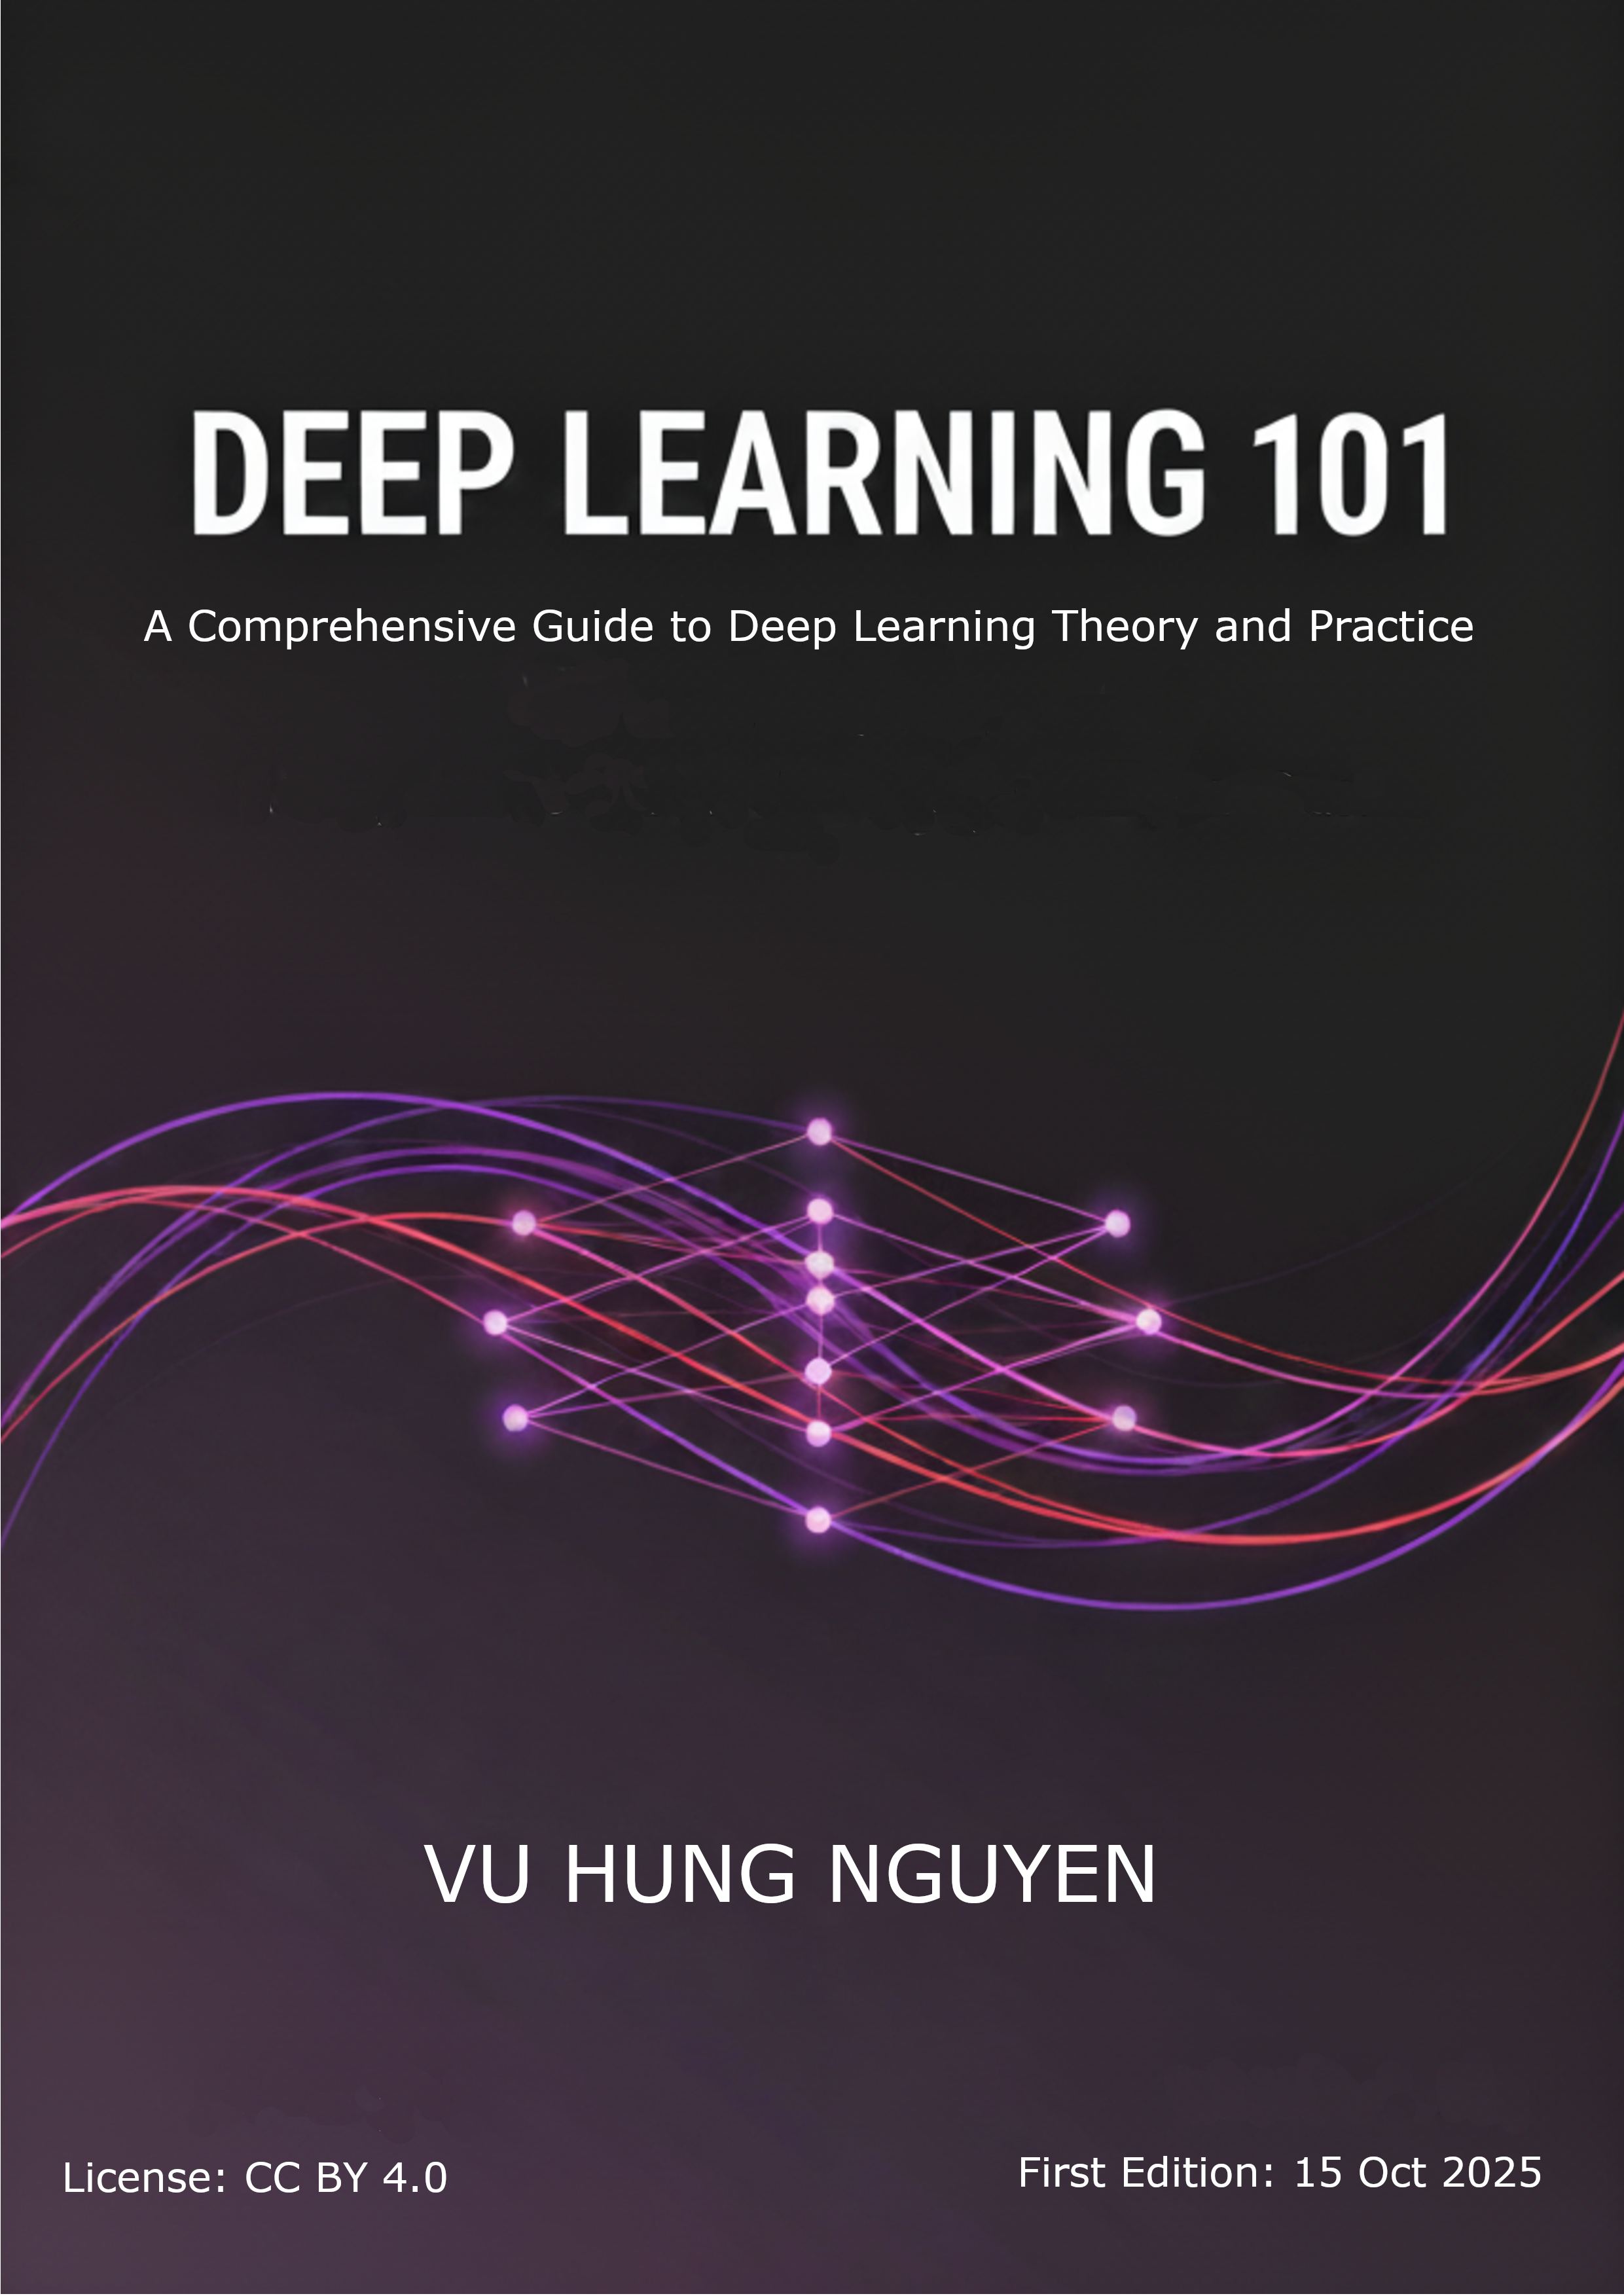
\includegraphics[width=\paperwidth,height=\paperheight]{images/DeepLearning101-cover-A4.png}%
    }{%
      \ifdefstring{\papersize}{a5paper}{%
        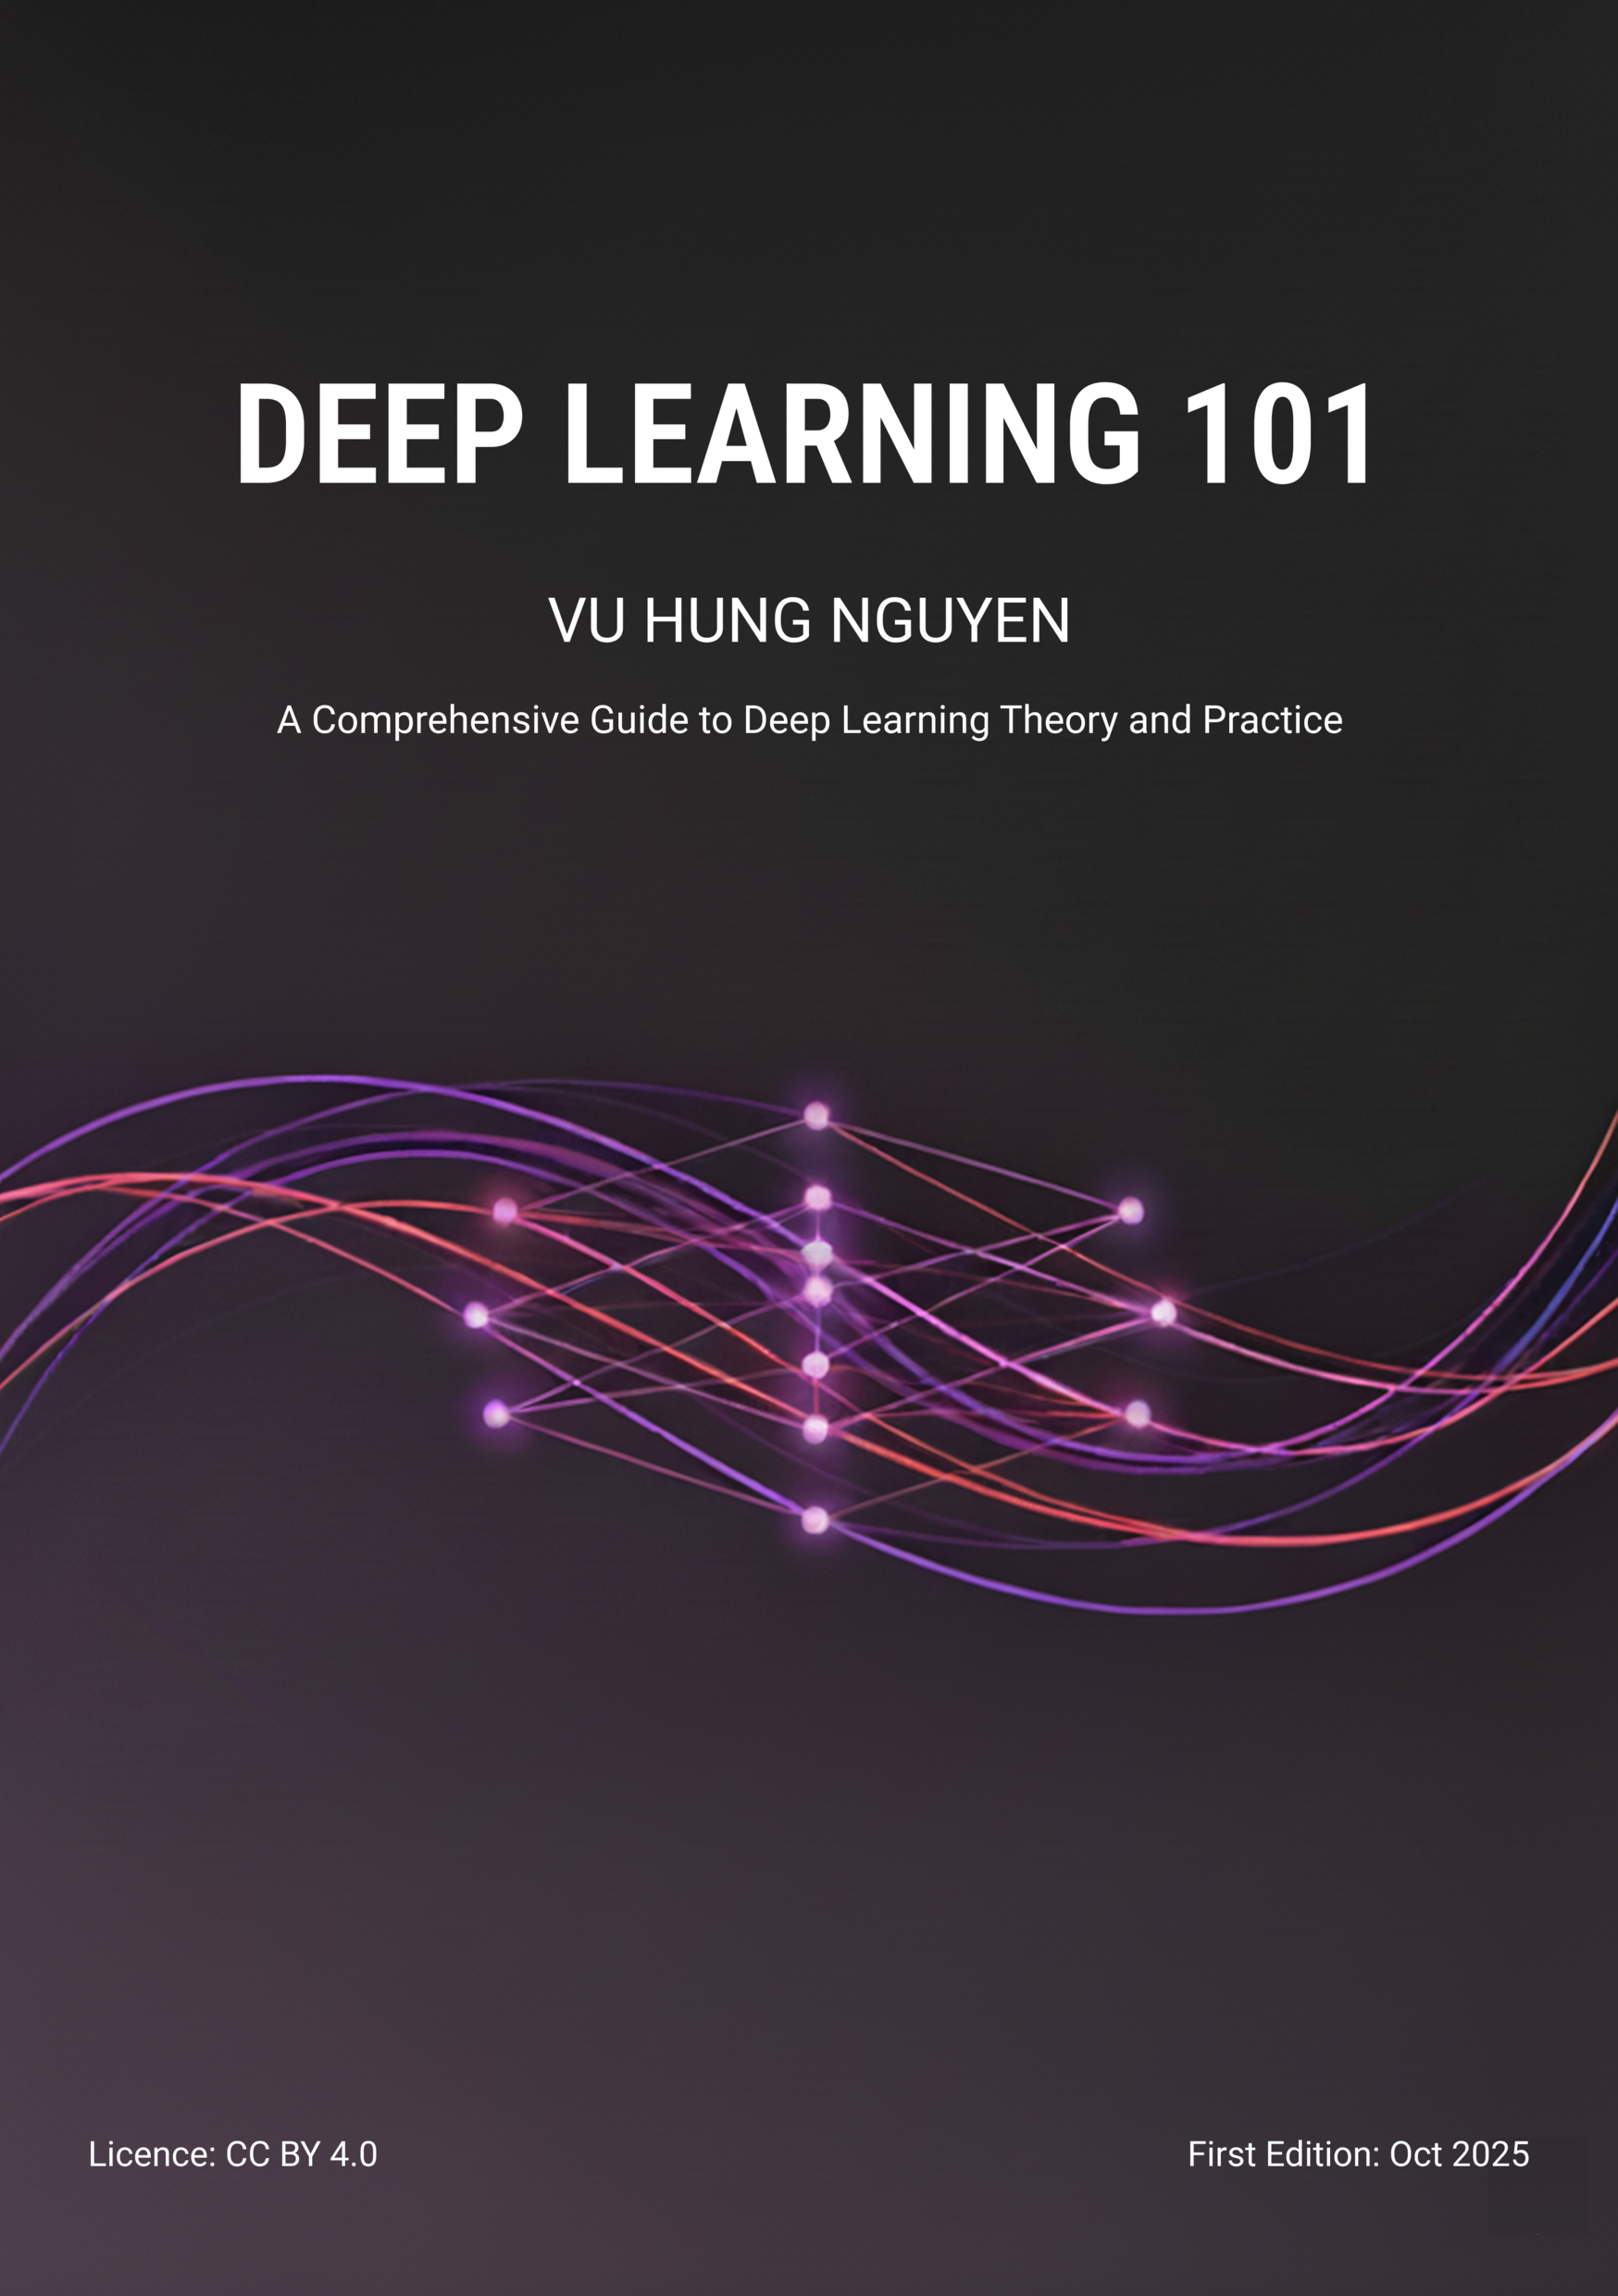
\includegraphics[width=\paperwidth,height=\paperheight]{images/DeepLearning101-cover-A5.png}%
      }{%
        \ifdefstring{\papersize}{letterpaper}{%
          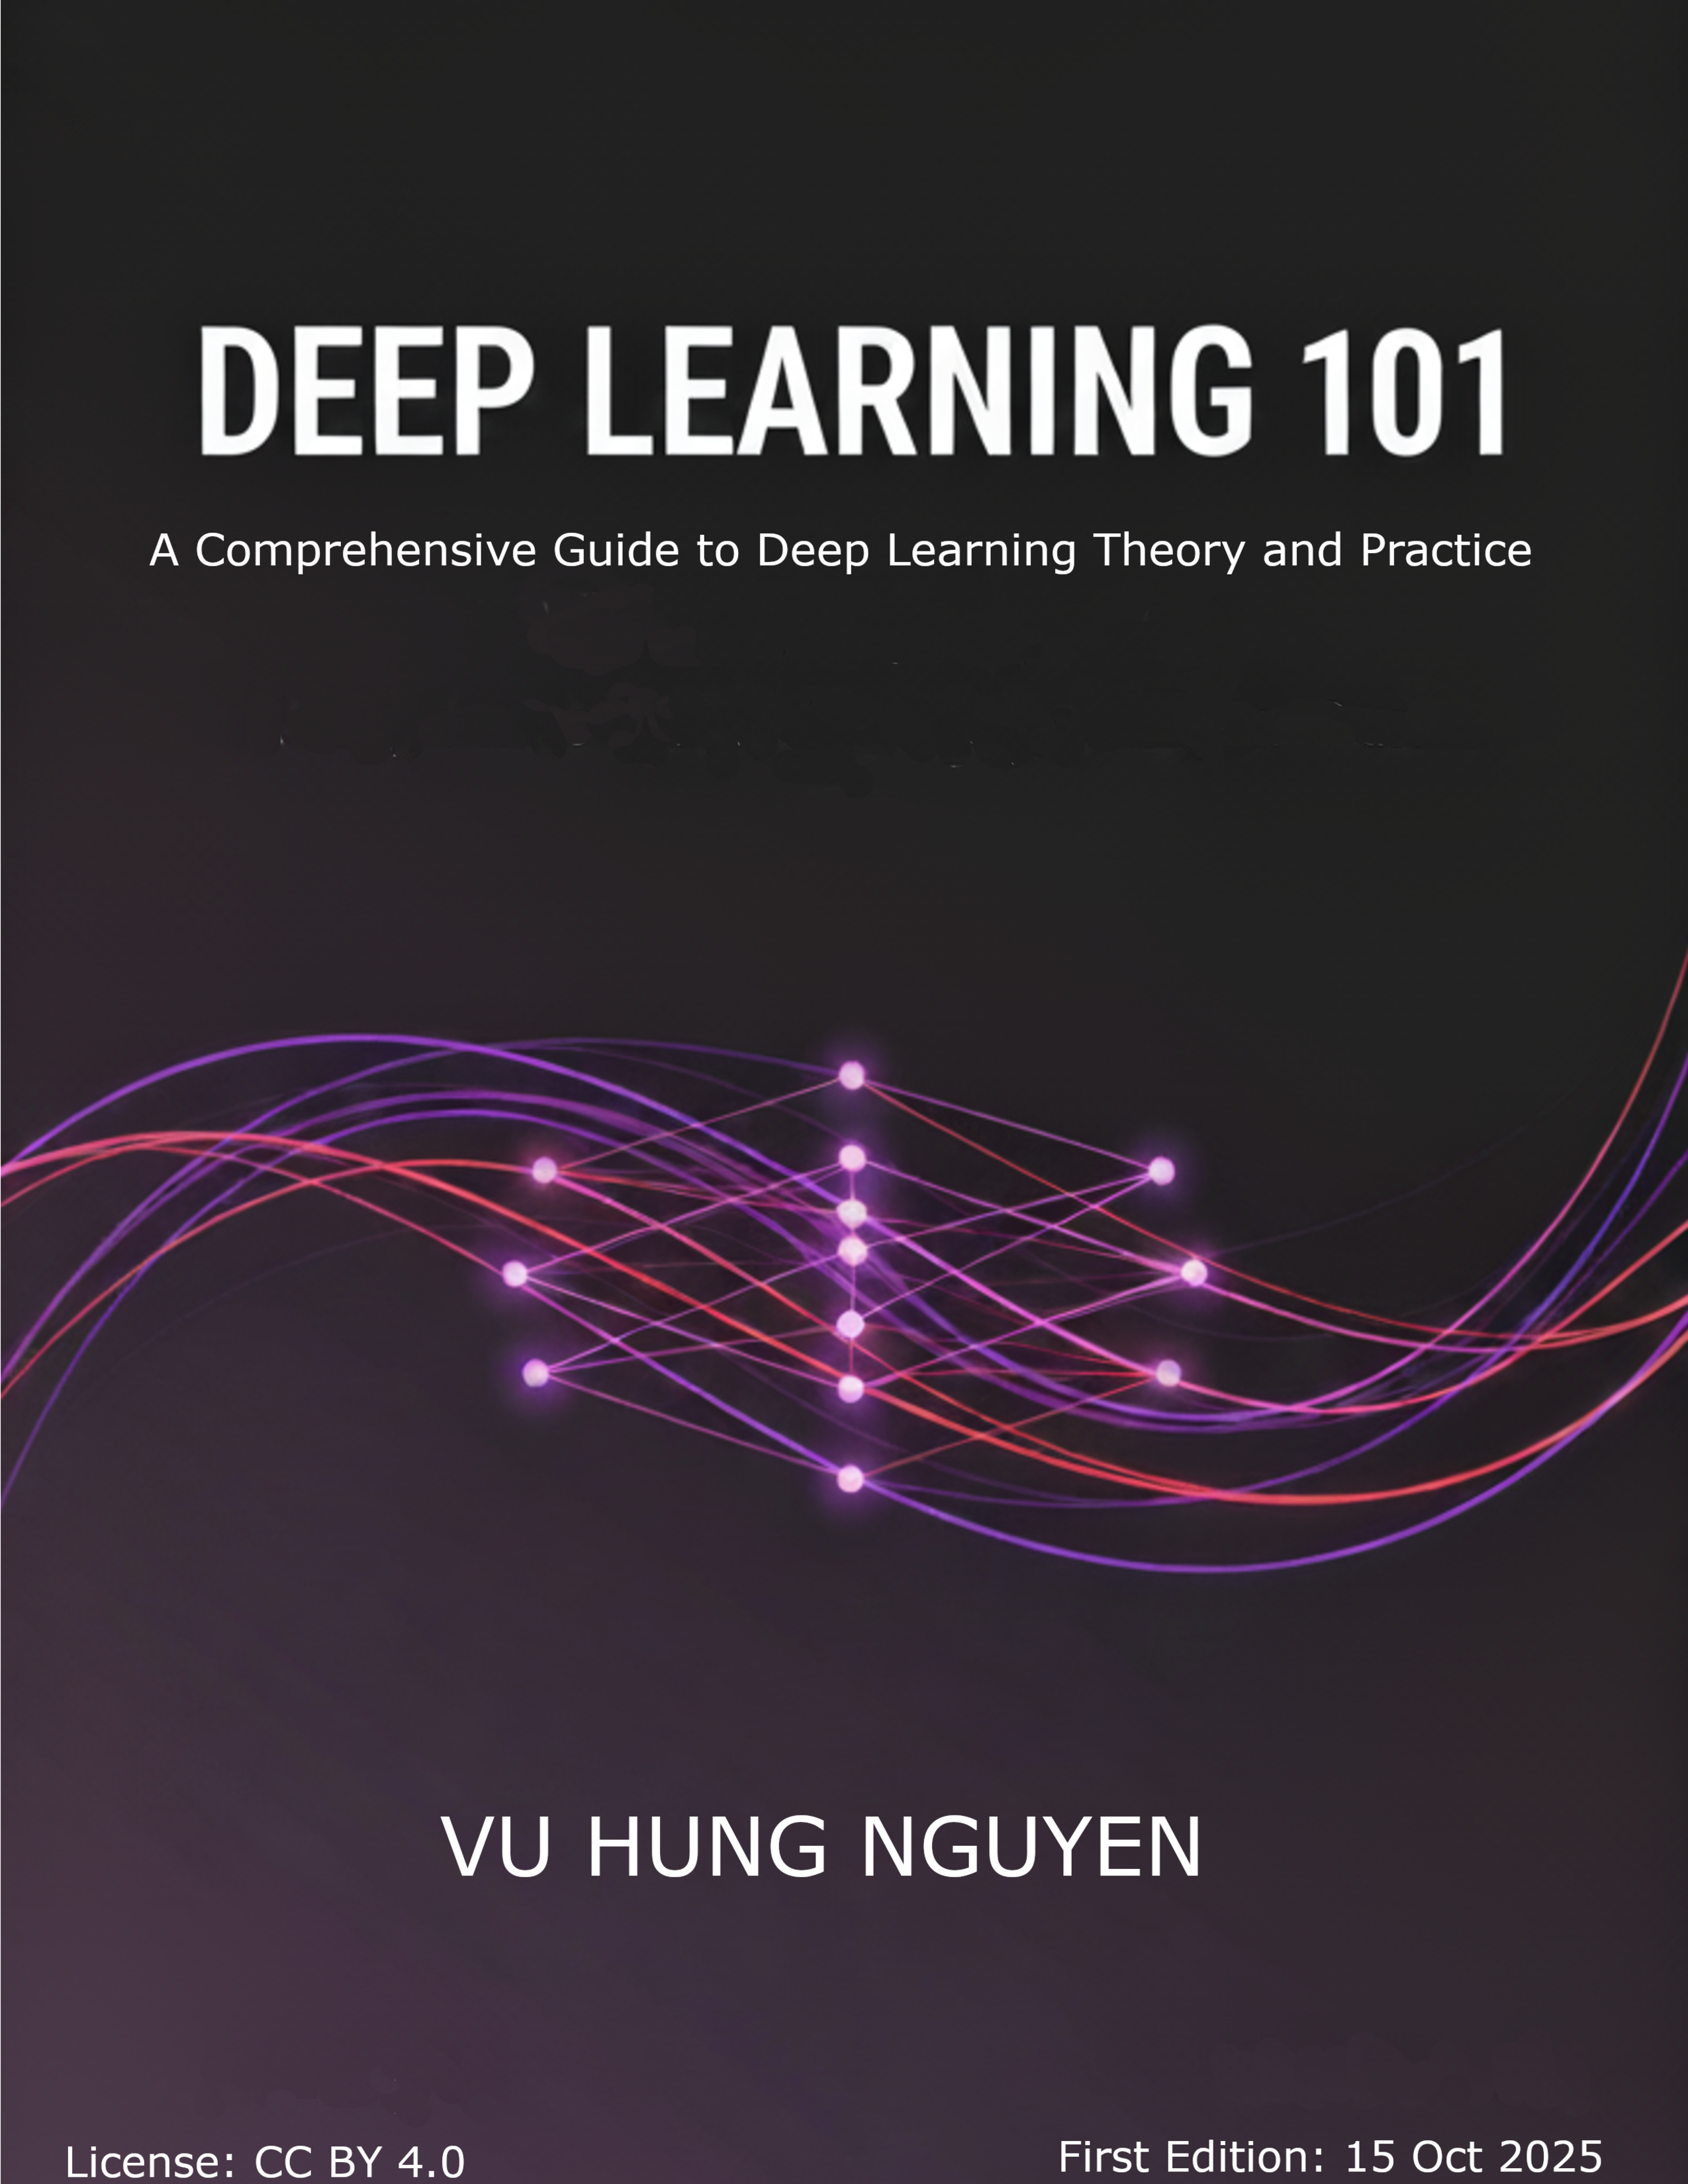
\includegraphics[width=\paperwidth,height=\paperheight]{images/DeepLearning101-cover-letter.png}%
        }{%
          \ifdefstring{\papersize}{a6paper}{%
            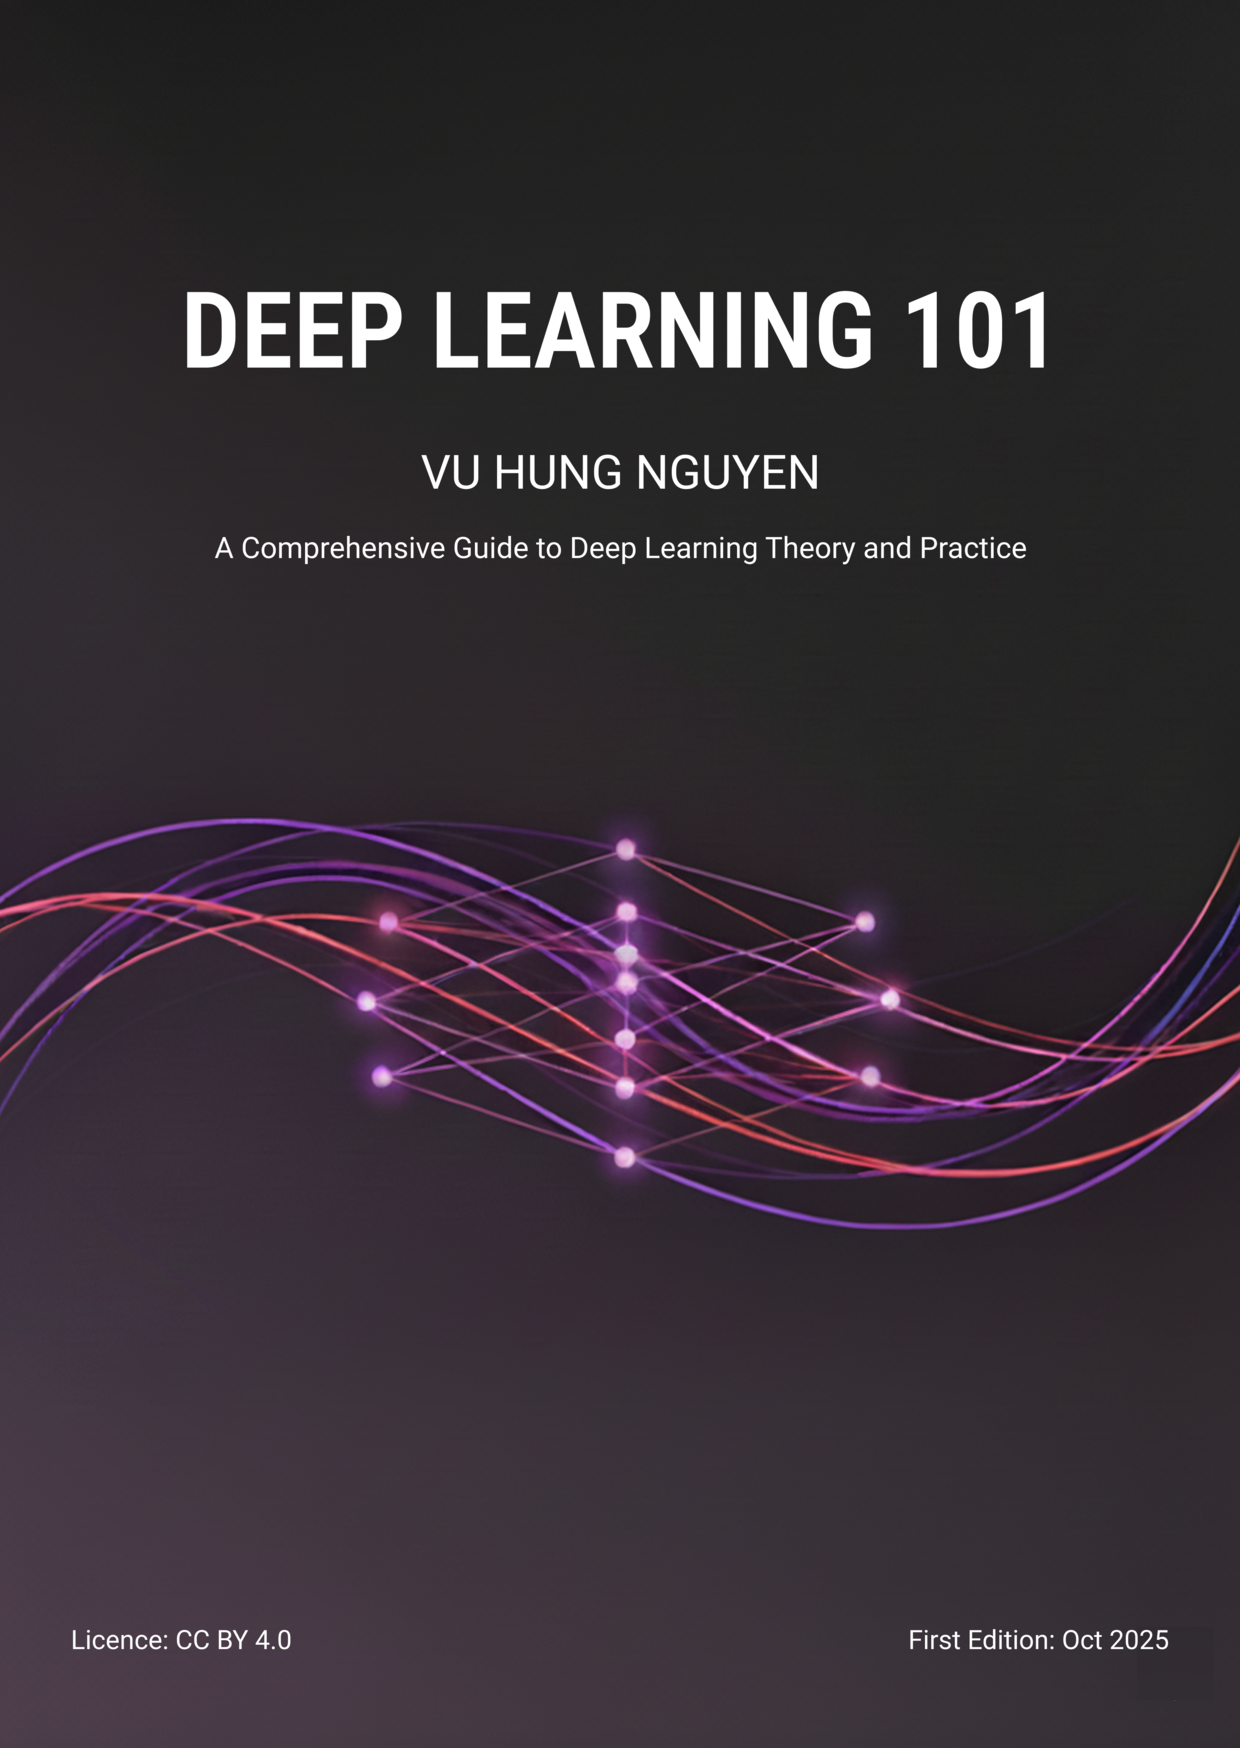
\includegraphics[width=\paperwidth,height=\paperheight]{images/DeepLearning101-cover-A6.png}%
          }{%
            \ifdefstring{\papersize}{b5paper}{%
              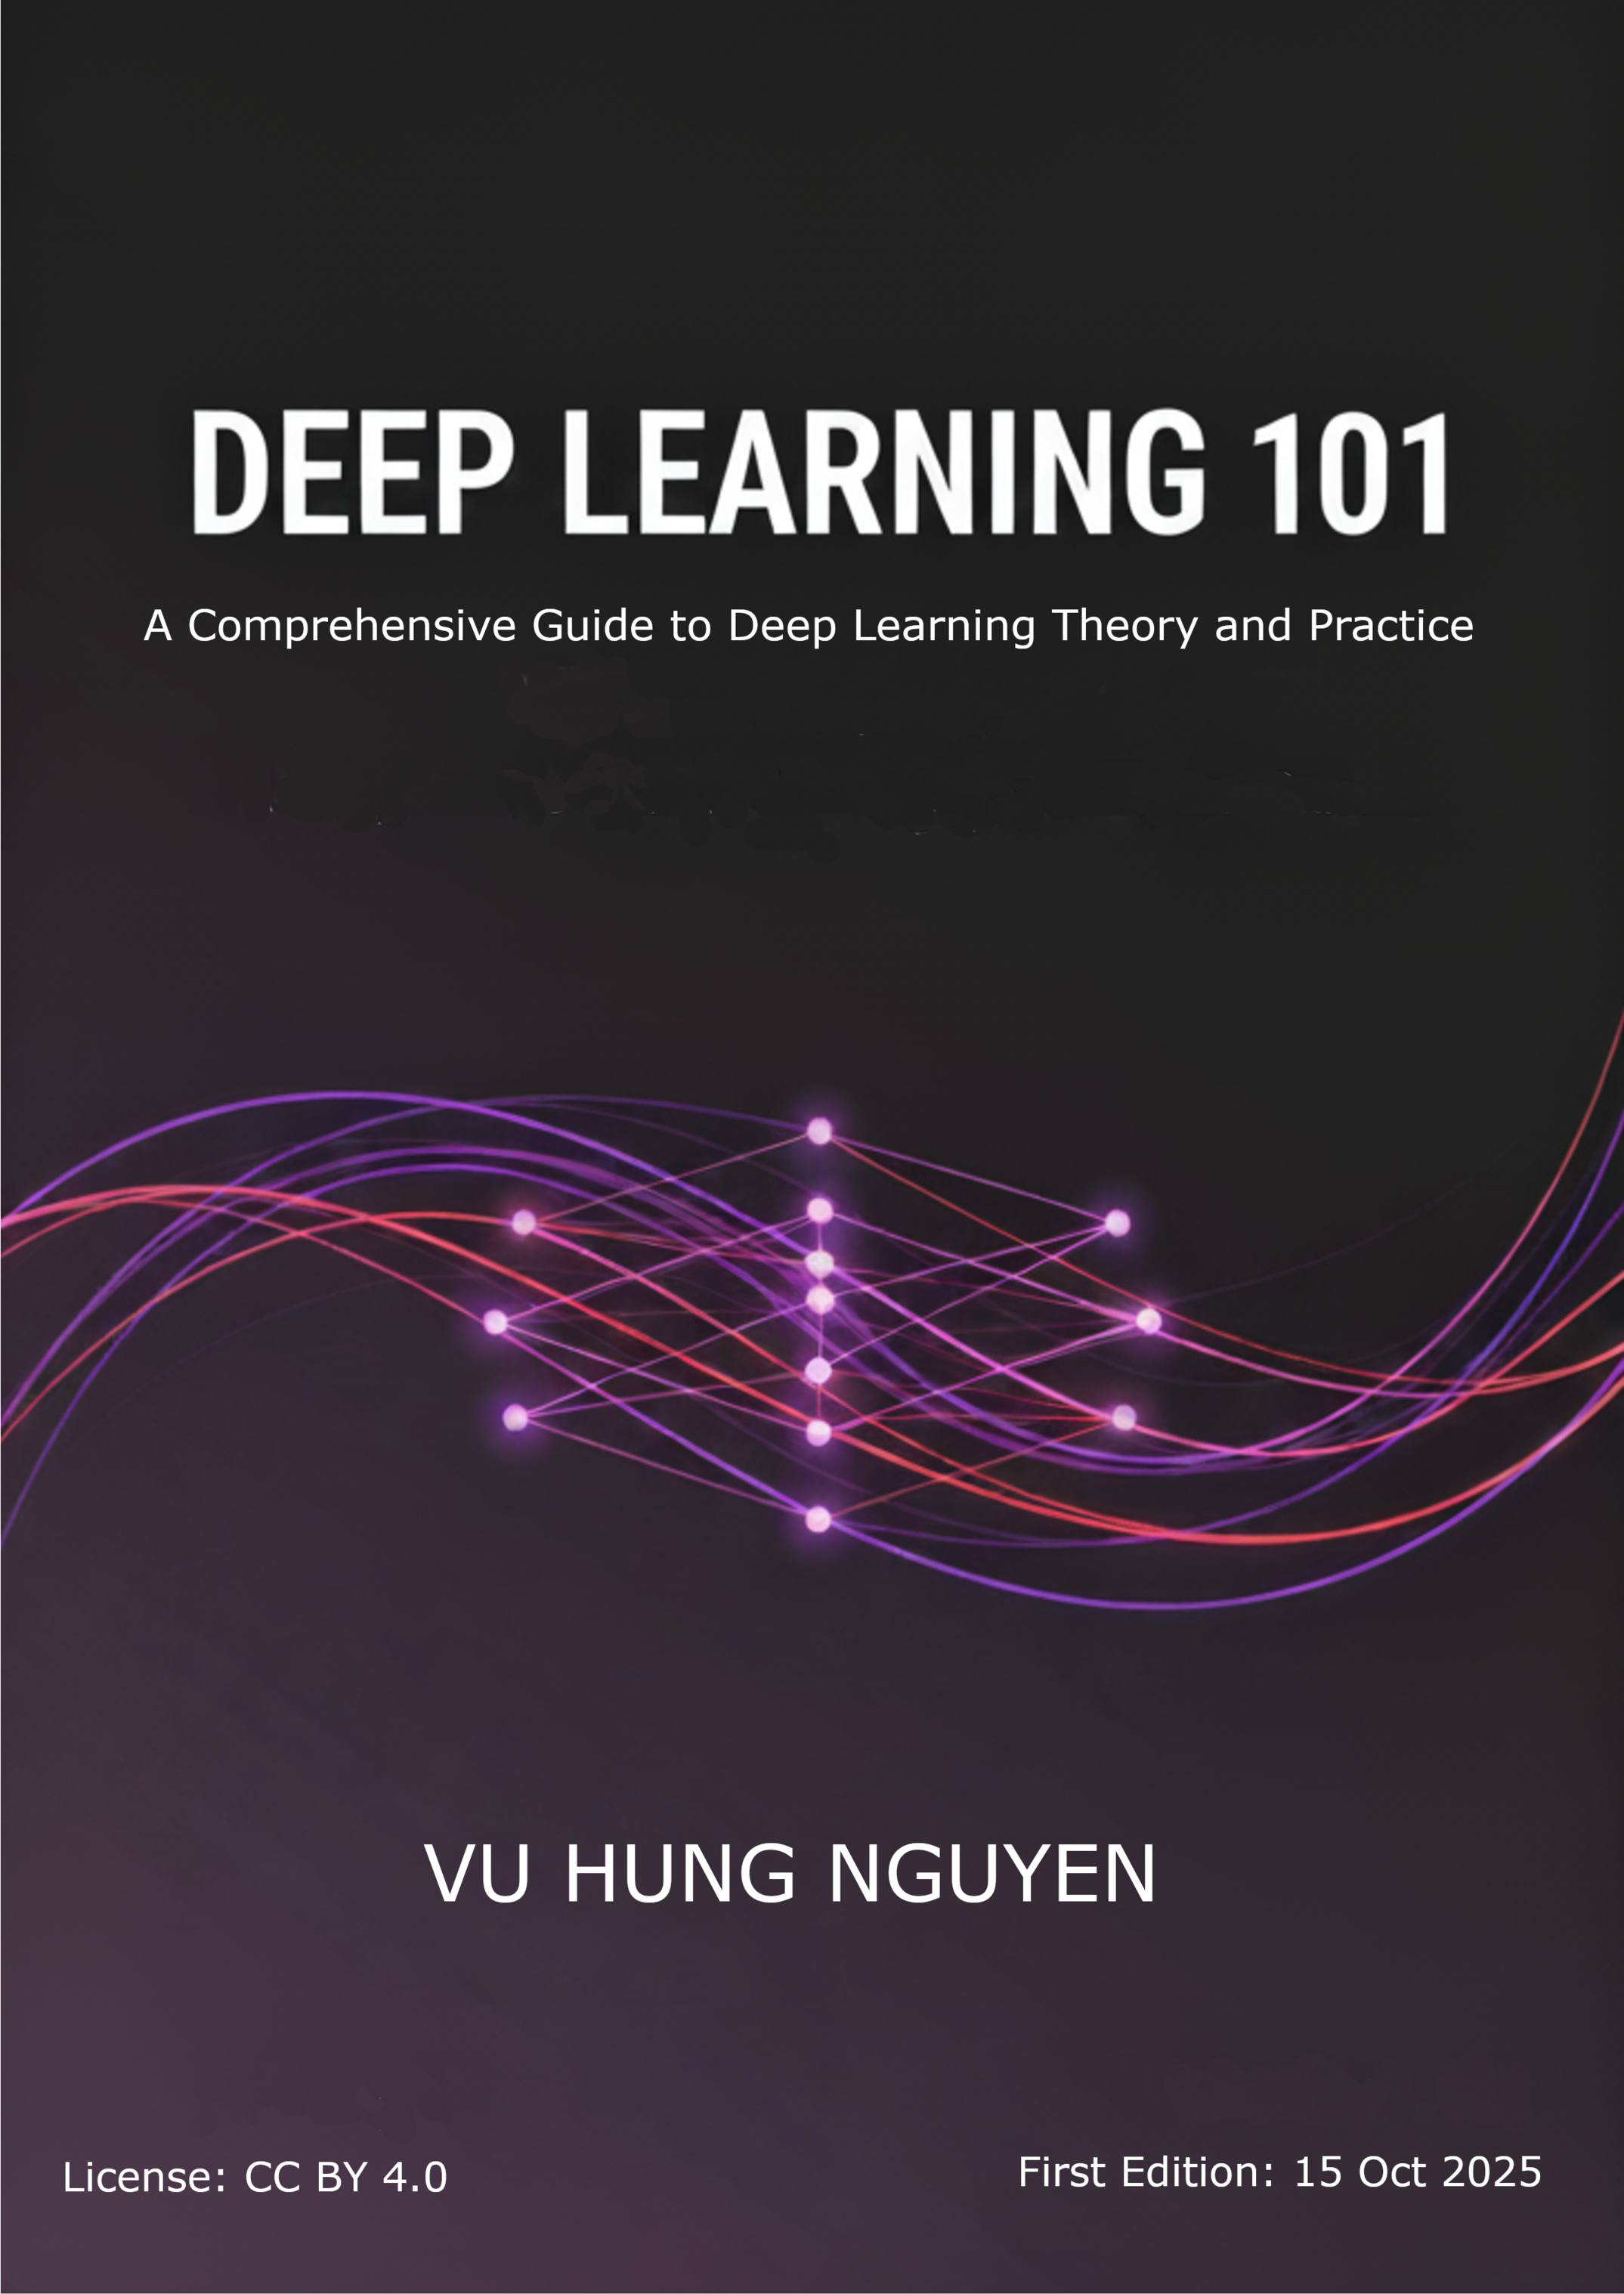
\includegraphics[width=\paperwidth,height=\paperheight]{images/DeepLearning101-cover-B5.png}%
            }{%
              \ifdefstring{\papersize}{trade}{%
                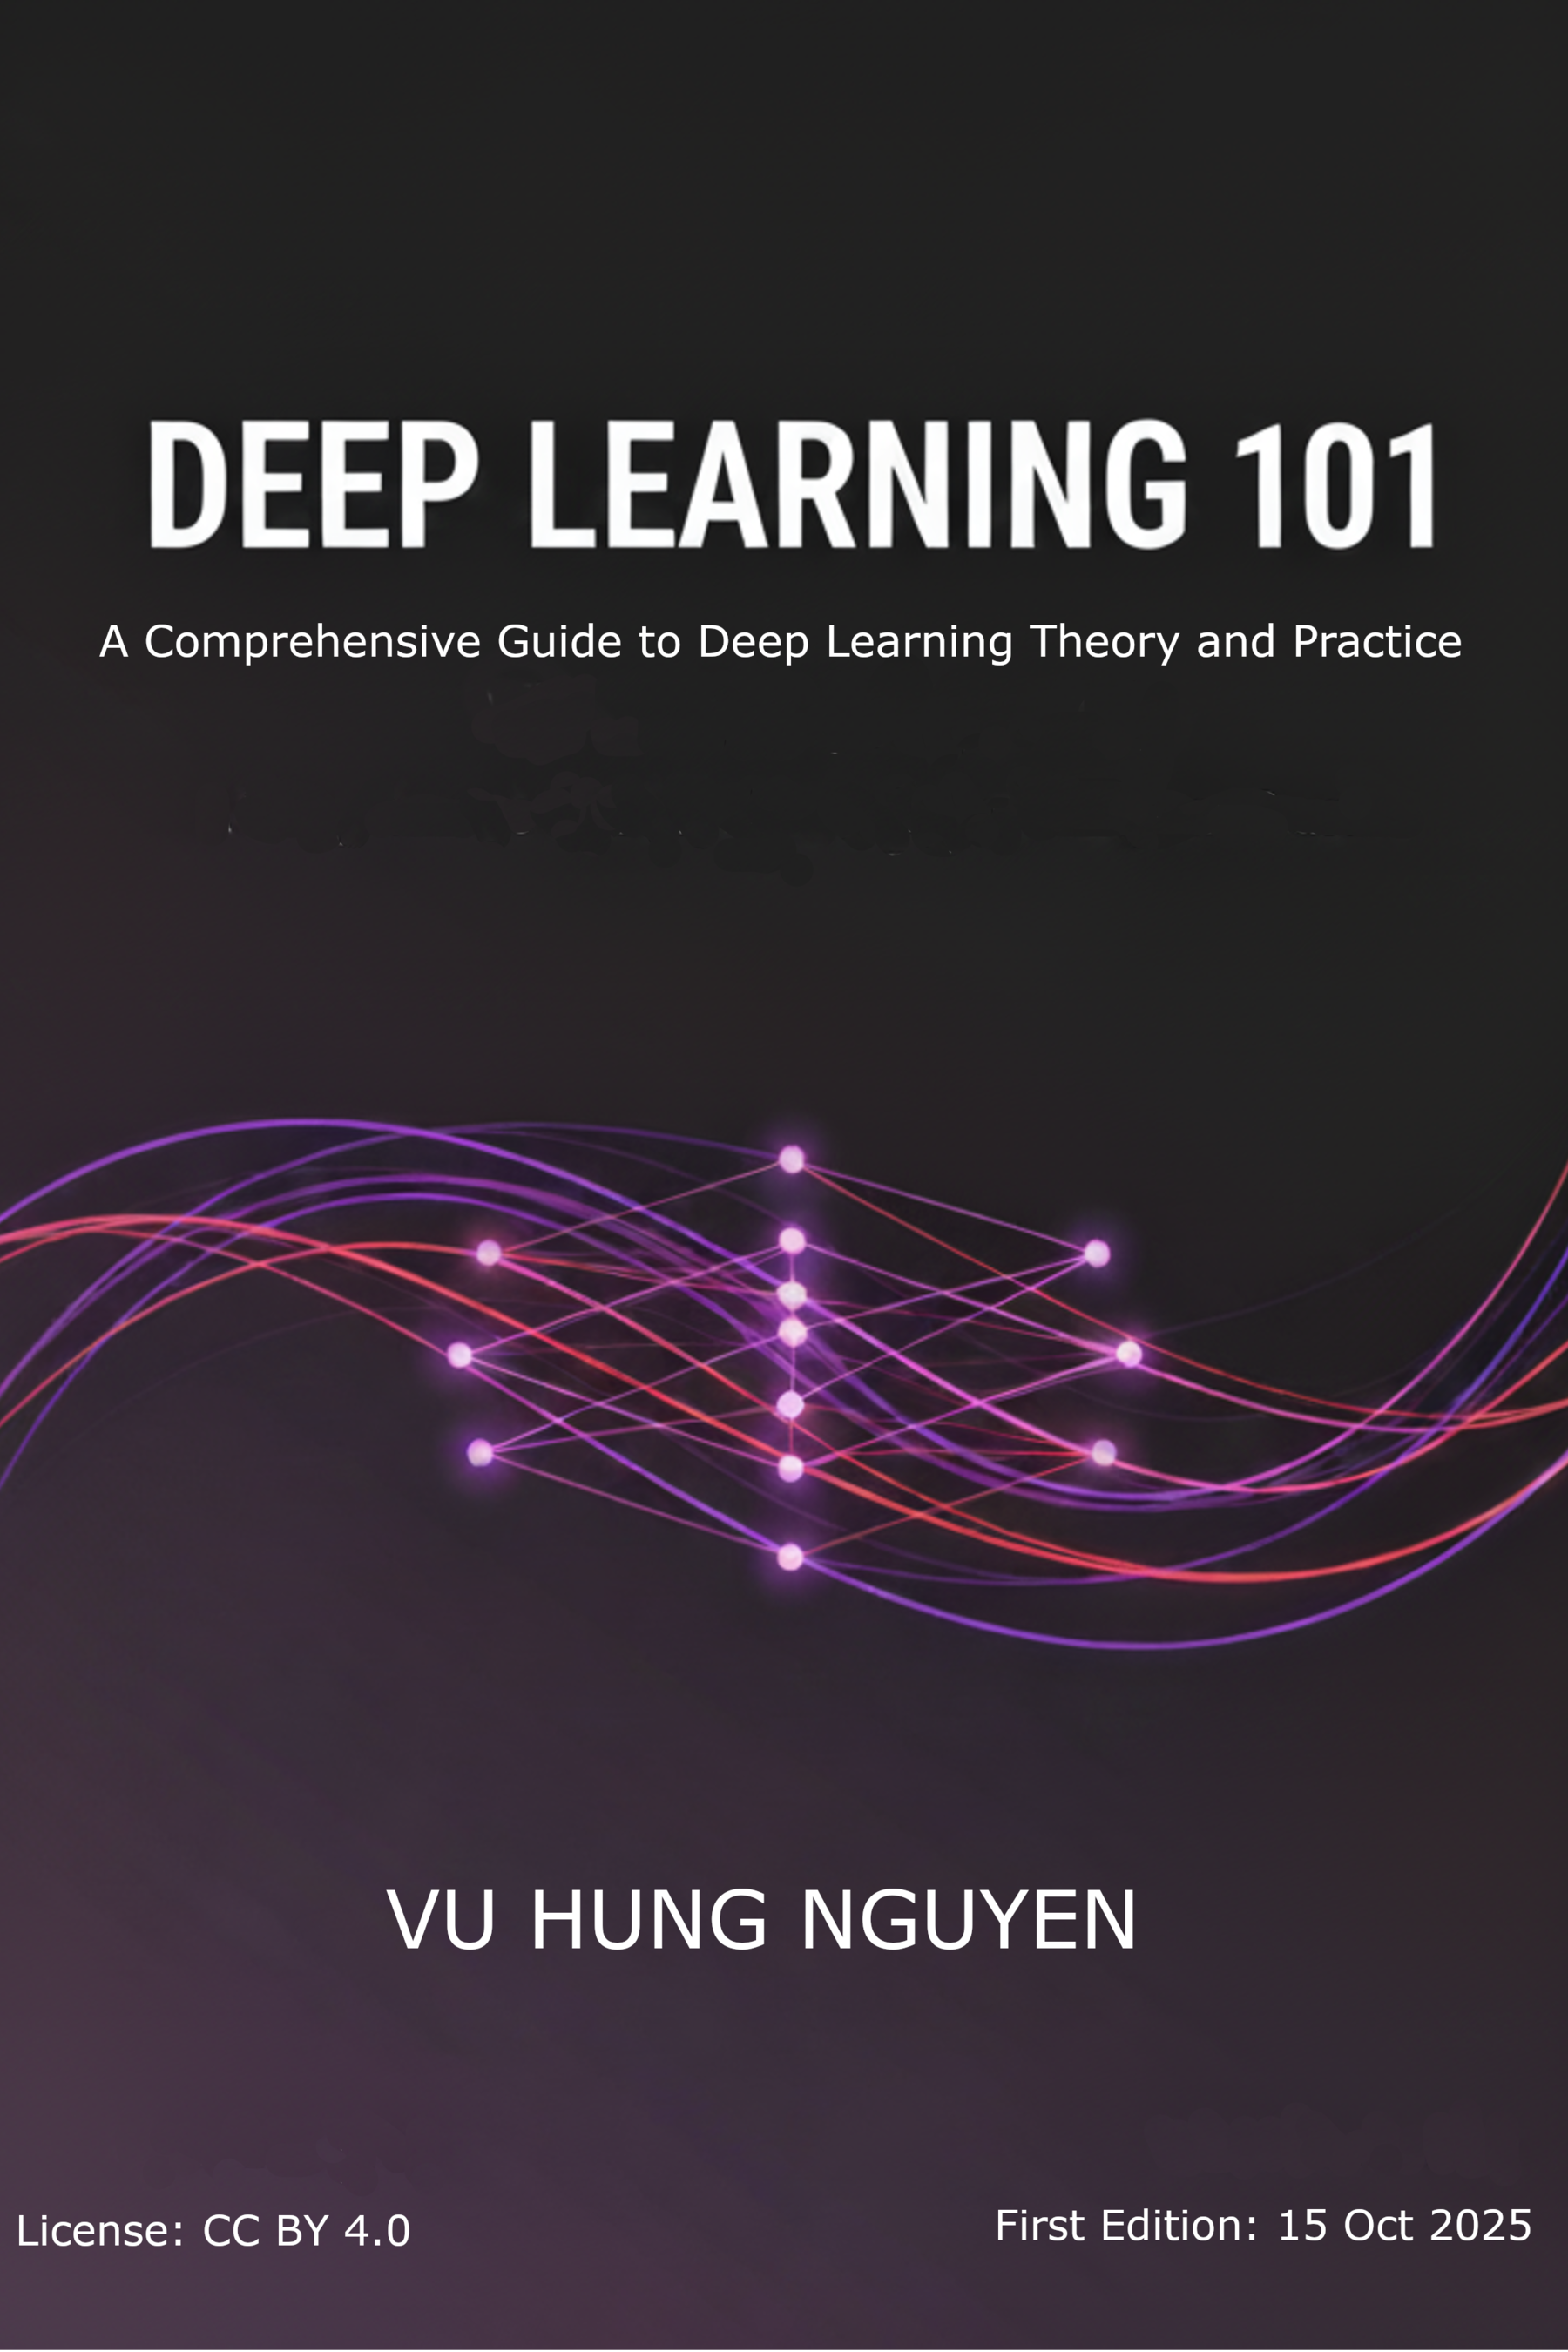
\includegraphics[width=\paperwidth,height=\paperheight]{images/DeepLearning101-cover-trade.png}%
              }{%
                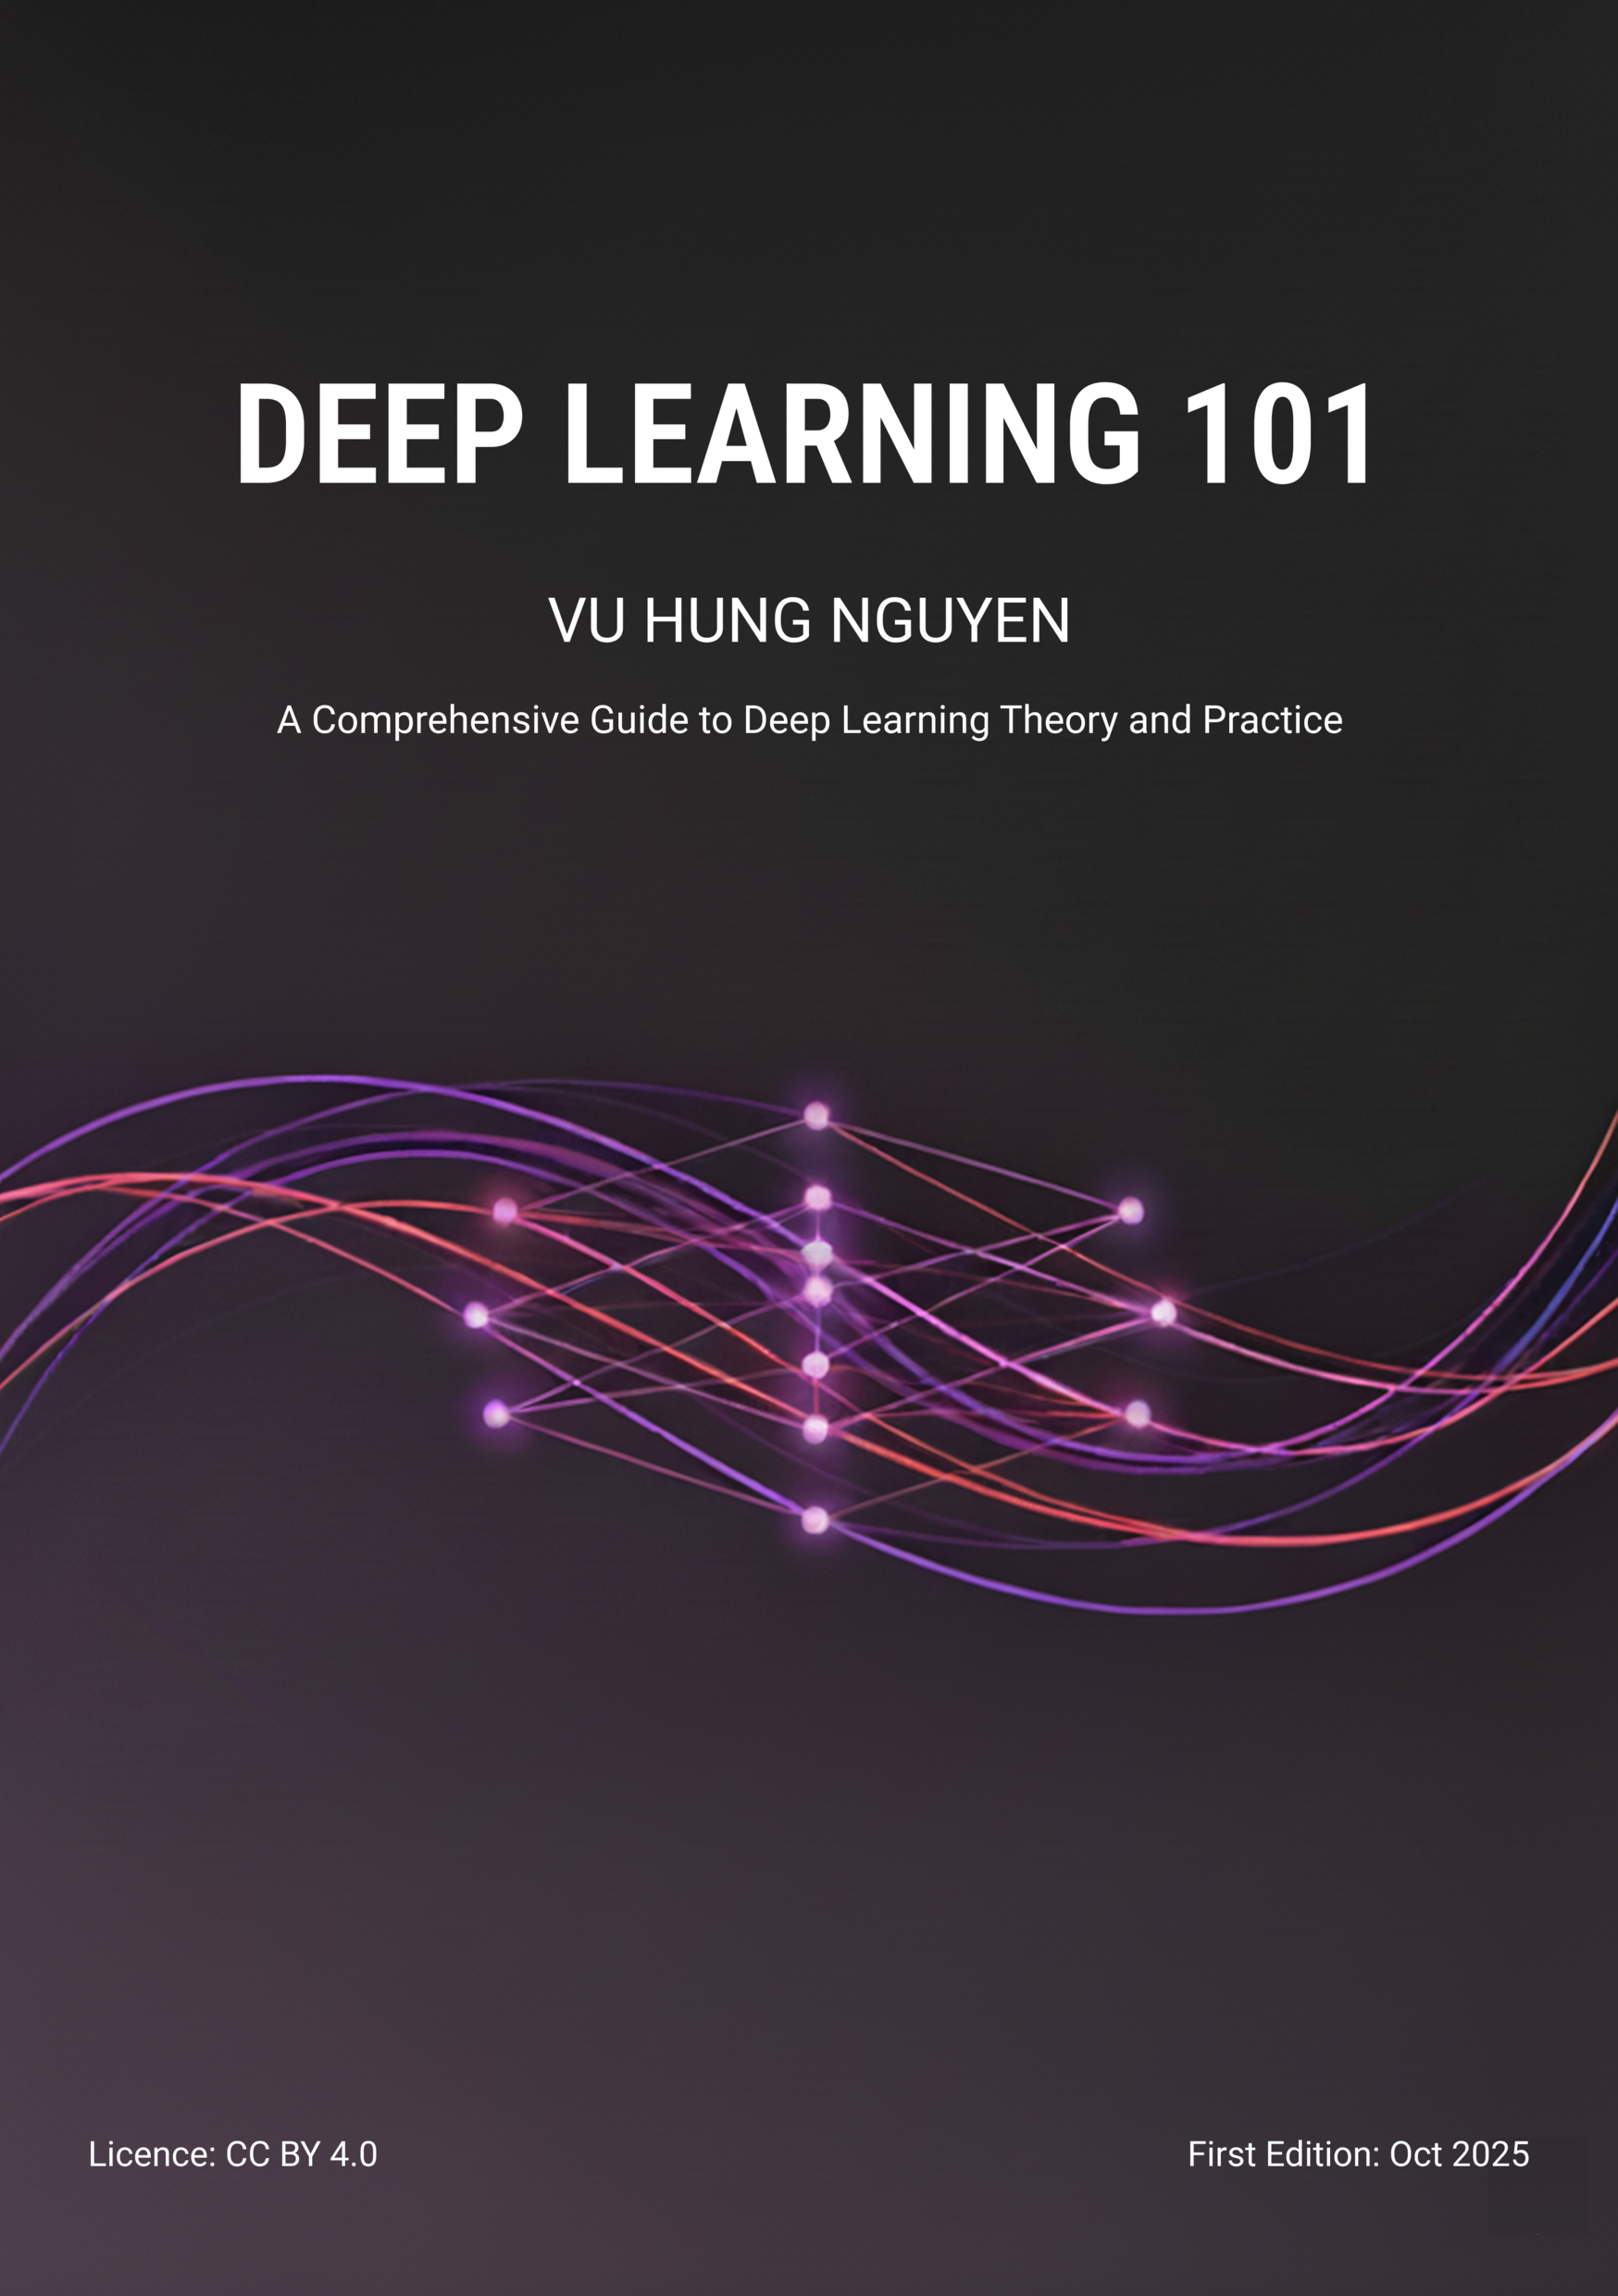
\includegraphics[width=\paperwidth,height=\paperheight]{images/DeepLearning101-cover-A5.png}%
              }%
            }%
          }%
        }%
      }%
    }%
  }%
}
\mbox{}% ensure a shipout
\endgroup % End the local scope, restoring previous margin settings
\clearpage

% Title Page - Text Content (Second Page)
\begin{titlepage}
\thispagestyle{empty}
\centering
\vspace*{\fill}

{\Huge\bfseries Deep Learning 101\par}
\vspace{2cm}

{\Large Nguyễn Vũ Hưng -- 阮武興 \par}
\vspace{2cm}

{\large A Comprehensive Guide to\\
Deep Learning Theory and Practice\par}

\vspace{3cm}

{\large \DTMtoday\par}
\vspace{1cm}

{\small License: Creative Commons Attribution 4.0 International (CC BY 4.0)\par}

\vspace*{\fill}
\end{titlepage}

% Copyright Page (Page 3)
\newpage
\thispagestyle{empty}
\vspace*{\fill}
\begin{flushleft}
\textbf{Deep Learning 101}\\
Copyright \copyright~\the\year~Vu Hung Nguyen\\[0.5em]
This work is licensed under the Creative Commons Attribution 4.0 International License.\\
To view a copy of this license, visit \url{http://creativecommons.org/licenses/by/4.0/}\\[0.5em]
First Edition: \DTMtoday
\end{flushleft}
\vspace*{\fill}
\clearpage

% Preface Page (Page 4)
\newpage
\thispagestyle{empty}
\vspace*{\fill}
\begin{flushleft}
\textbf{Preface}\\[1em]

Dear ML/AI learners,\\[0.5em]

Welcome to \textit{Deep Learning 101}, a comprehensive guide designed to take you from the fundamentals to advanced concepts in deep learning. This book is crafted for students, researchers, and practitioners who want to build a solid foundation in one of the most transformative fields of our time.\\[0.5em]

I started this book as study notes for myself, because I couldn't find any book that fit my background. As I delved deeper into the field, I realised that many existing resources were either too basic or too advanced, leaving a gap for learners with a technical foundation seeking comprehensive yet accessible coverage.\\[0.5em]

This book is a ``compressed version'' of the deep learning books out there---you'll find the most important concepts and mathematical formulae presented in a structured, coherent manner. Rather than overwhelming you with every detail, I've distilled the essential knowledge that forms the foundation of modern deep learning.\\[0.5em]

This book assumes you have a fair understanding of mathematics, algorithms, and programming. But don't worry---you'll learn along the way if you miss any of them. The early chapters provide mathematical foundations, and examples throughout the book will help reinforce concepts you may need to review.\\[0.5em]

The target audience includes those who want to learn the basics of deep learning with a focus on mathematics. If you're interested in research or want to dive a little deeper into the maths and algorithms underlying neural networks, this book will guide you through both theory and practice.\\[0.5em]

Whether you're just beginning your journey into machine learning or looking to deepen your understanding of neural networks, this book provides the mathematical foundations, practical insights, and hands-on knowledge you need to succeed.\\[0.5em]

I hope this resource serves you well in your learning journey.\\[1em]

Best regards,\\
Vu Hung Nguyen\\[1em]

\textbf{Contact Information:}\\
GitHub: \url{https://github.com/vuhung16au}\\
LinkedIn: \url{https://www.linkedin.com/in/nguyenvuhung/}\\
Website: \url{https://vuhung16au.github.io/}
\end{flushleft}
\vspace*{\fill}
\clearpage

% --- Front Matter ---
% Now start front matter after cover and title pages
% Reset page numbering for front matter
\setcounter{page}{1}
\pagenumbering{roman}
\frontmatter

% Table of Contents
\tableofcontents

% Acknowledgements
\chapter*{Acknowledgements}
\addcontentsline{toc}{chapter}{Acknowledgements}
I would like to express my deepest gratitude to the deep learning community for their invaluable contributions to this rapidly evolving field. Special thanks to the pioneers whose groundbreaking work laid the foundation for modern deep learning.

I am grateful to my colleagues, students, and collaborators who have provided feedback, suggestions, and encouragement throughout the writing of this book. Your insights have been instrumental in shaping the content and presentation of this material.

This book draws inspiration from the excellent resources available in the deep learning community, including the seminal work by Goodfellow, Bengio, and Courville, as well as the emerging literature on understanding deep learning.

I would also like to thank my family for their unwavering support and patience during the many hours spent writing and revising this manuscript.

Finally, I am grateful to all readers who engage with this material and contribute to the advancement of deep learning through their research, applications, and education.

Any errors or omissions in this book are entirely my own responsibility.


\vspace{1cm}
\noindent Vu Hung Nguyen\\
\today


% Notation
\chapter*{Notation}
\addcontentsline{toc}{chapter}{Notation}
This book uses the following notation throughout:

\section*{General Notation}

\begin{itemize}[leftmargin=2em]
    \item $a, b, c$ --- scalars (lowercase italic letters)
    \item $\vect{a}, \vect{b}, \vect{c}$ --- vectors (bold lowercase letters)
    \item $\mat{A}, \mat{B}, \mat{C}$ --- matrices (bold uppercase letters)
    \item $\mathcal{A}, \mathcal{B}, \mathcal{C}$ --- sets (calligraphic uppercase)
    \item $a_i$ --- the $i$-th element of vector $\vect{a}$
    \item $A_{ij}$ or $\mat{A}_{ij}$ --- element at row $i$, column $j$ of matrix $\mat{A}$
    \item $\mat{A}\transpose$ --- transpose of matrix $\mat{A}$
    \item $\mat{A}^{-1}$ --- inverse of matrix $\mat{A}$
    \item $\norm{\vect{x}}$ --- norm of vector $\vect{x}$ (typically $L^2$ norm)
    \item $\norm{\vect{x}}_p$ --- $L^p$ norm of vector $\vect{x}$
    \item $\abs{x}$ --- absolute value of scalar $x$
    \item $\mathbb{R}$ --- set of real numbers
    \item $\mathbb{R}^n$ --- $n$-dimensional real vector space
    \item $\mathbb{R}^{m \times n}$ --- set of real $m \times n$ matrices
    \item $\mathbb{E}$ --- expectation operator
    \item $\mathbb{P}$ --- probability measure
    \item $\mathbb{N}$ --- set of natural numbers
    \item $\mathbb{Z}$ --- set of integers
    \item $\mathbb{C}$ --- set of complex numbers
\end{itemize}

\section*{Probability and Statistics}

\begin{itemize}[leftmargin=2em]
    \item $P(X)$ --- probability distribution over discrete variable $X$
    \item $p(x)$ --- probability density function over continuous variable $x$
    \item $P(X=x)$ or $P(x)$ --- probability that $X$ takes value $x$
    \item $P(X|Y)$ --- conditional probability of $X$ given $Y$
    \item $\mathbb{E}_{x \sim P}[f(x)]$ --- expectation of $f(x)$ with respect to distribution $P$
    \item $\text{Var}(X)$ --- variance of random variable $X$
    \item $\text{Cov}(X, Y)$ --- covariance of random variables $X$ and $Y$
    \item $\mathcal{N}(\mu, \sigma^2)$ --- Gaussian distribution with mean $\mu$ and variance $\sigma^2$
    \item $\mathcal{L}$ --- loss function or likelihood
    \item $\mathcal{J}$ --- cost function or objective function
    \item $\mathcal{H}$ --- Hessian matrix or Hamiltonian
    \item $\mathcal{D}$ --- dataset or domain
    \item $\mathcal{M}$ --- manifold or model space
\end{itemize}

\section*{Calculus and Optimization}

\begin{itemize}[leftmargin=2em]
    \item $\frac{dy}{dx}$ or $\frac{\partial y}{\partial x}$ --- derivative of $y$ with respect to $x$
    \item $\nabla_{\vect{x}} f$ --- gradient of function $f$ with respect to $\vect{x}$
    \item $\nabla^2 f$ or $\mat{H}$ --- Hessian matrix (matrix of second derivatives)
    \item $\arg\min_x f(x)$ --- value of $x$ that minimizes $f(x)$
    \item $\arg\max_x f(x)$ --- value of $x$ that maximizes $f(x)$
\end{itemize}

\section*{Machine Learning}

\begin{itemize}[leftmargin=2em]
    \item $\mathcal{D}$ --- dataset
    \item $\mathcal{D}_{\text{train}}$ --- training dataset
    \item $\mathcal{D}_{\text{val}}$ --- validation dataset
    \item $\mathcal{D}_{\text{test}}$ --- test dataset
    \item $n$ --- number of examples in dataset
    \item $m$ --- mini-batch size
    \item $\vect{x}$ --- input vector or feature vector
    \item $y$ --- target or label
    \item $\hat{y}$ --- prediction or estimated output
    \item $\vect{\theta}$ or $\vect{w}$ --- parameters or weights
    \item $\mathcal{L}$ --- loss function
    \item $J$ --- cost function (sum or average of losses)
    \item $\alpha$ or $\eta$ --- learning rate
    \item $\lambda$ --- regularization coefficient
\end{itemize}

\section*{Neural Networks}

\begin{itemize}[leftmargin=2em]
    \item $L$ --- number of layers in a neural network
    \item $n^{[l]}$ --- number of units in layer $l$
    \item $\vect{a}^{[l]}$ --- activations of layer $l$
    \item $\vect{z}^{[l]}$ --- pre-activation values of layer $l$
    \item $\mat{W}^{[l]}$ --- weight matrix for layer $l$
    \item $\vect{b}^{[l]}$ --- bias vector for layer $l$
    \item $f$ or $\sigma$ --- activation function
    \item $g$ --- general function or transformation
    \item $\vect{h}$ --- hidden state or intermediate representation
    \item $\vect{z}$ --- latent variable or pre-activation
    \item $\vect{s}$ --- state vector or score
    \item $\vect{e}$ --- embedding vector or error
    \item $\vect{r}$ --- residual or reward
\end{itemize}

\subsection*{Difficulty Legend}
\addcontentsline{toc}{subsection}{Difficulty Legend}

\begin{description}[leftmargin=2.2em,labelsep=0.6em]
  \item[\difficultyBeginner\ Beginner] Intuition-first explanations; minimal prerequisites.
  \item[\difficultyIntermediate\ Intermediate] Assumes fundamentals; technical details and derivations.
  \item[\difficultyAdvanced\ Advanced] Research-level topics or heavier mathematics.
\end{description}


% --- Main Matter ---
\mainmatter

% Chapter 1: Introduction
% Chapter 1: Introduction

\chapter{Introduction}
\label{chap:introduction}

This chapter introduces the fundamental concepts of deep learning and its historical context, providing a foundation for understanding the field.

\begin{learningobjectives}
\objective{Deep learning concepts and differences from traditional machine learning}
\objective{Historical development of neural networks and key breakthroughs}
\objective{Major application domains where deep learning has achieved success}
\objective{Key factors that enabled the rise of deep learning in the 21st century}
\objective{Challenges and limitations of deep learning approaches}
\end{learningobjectives}



% Chapter 1, Section 1: What is Deep Learning?

\section{What is Deep Learning? \difficultyInline{beginner}}
\label{sec:what-is-dl}

Deep learning is a subfield of machine learning that focuses on learning hierarchical representations of data through artificial \gls{neural-network}s with multiple layers. These networks, inspired by the structure and function of the human brain, have revolutionized numerous fields including \gls{computer-vision}, \gls{natural-language-processing}, speech recognition, and many others.

\subsection{The Rise of Deep Learning}

The resurgence of neural networks, now known as deep learning, can be attributed to several key factors:

\begin{enumerate}
    \item \textbf{Availability of Large Datasets:} The digital age has produced massive amounts of data, providing the fuel needed to train complex models effectively.
    
    \item \textbf{Computational Power:} The advent of Graphics Processing Units (GPUs) and specialized hardware has enabled the training of much larger networks than was previously possible.
    
    \item \textbf{Algorithmic Innovations:} Improvements in optimization algorithms, regularization techniques, and network architectures have made it possible to train very deep networks.
    
    \item \textbf{Open-Source Software:} Frameworks like TensorFlow, PyTorch, and others have democratized access to deep learning tools.
\end{enumerate}

\subsection{Key Characteristics}

Deep learning differs from traditional machine learning in several important ways:

\begin{itemize}
    \item \textbf{Automatic Feature Learning:} Unlike traditional approaches that require manual feature engineering, deep learning models automatically learn relevant features from raw data.
    
    \item \textbf{Hierarchical Representations:} Deep networks learn multiple levels of representation, from low-level features (e.g., edges in images) to high-level concepts (e.g., object categories).
    
    \item \textbf{End-to-End Learning:} Deep learning often enables end-to-end learning, where the entire system is trained jointly rather than in separate stages.
    
    \item \textbf{Scalability:} Deep learning models can continue to improve with more data and computational resources.
\end{itemize}

\subsection{Applications}

Deep learning has achieved remarkable success in numerous domains:

\begin{description}
    \item[Computer Vision:] Image classification, object detection, semantic segmentation, facial recognition, and image generation.
    
    \item[Natural Language Processing:] Machine translation, sentiment analysis, question answering, text generation, and language understanding.
    
    \item[Speech and Audio:] Speech recognition, speaker identification, music generation, and audio synthesis.
    
    \item[Healthcare:] Medical image analysis, drug discovery, disease prediction, and personalized medicine.
    
    \item[Robotics:] Autonomous navigation, manipulation, and decision-making.
    
    \item[Game Playing:] Achieving superhuman performance in complex games like Go, Chess, and video games.
\end{description}

The impact of deep learning extends far beyond these applications, touching virtually every aspect of modern technology and scientific research.

% Index entries
\index{deep learning!introduction}
\index{machine learning!deep learning}
\index{neural networks!deep learning}
\index{artificial intelligence!deep learning}

% Chapter 1, Section 2: Historical Context

\section{Historical Context \difficultyInline{beginner}}
\label{sec:historical-context}

The history of deep learning is intertwined with the broader history of artificial intelligence and neural networks. Understanding this context helps us appreciate the current state of the field and its future directions.

\subsection{The Perceptron Era (1940s-1960s)}

The foundations of neural networks were laid in the 1940s with the work of Warren McCulloch and Walter Pitts, who created a computational model of a neuron. In 1958, Frank Rosenblatt invented the Perceptron, an algorithm for learning a binary classifier.

The Perceptron showed promise but faced significant limitations. In 1969, Marvin Minsky and Seymour Papert's book \emph{Perceptrons} demonstrated that single-layer perceptrons could not solve non-linearly separable problems like XOR, leading to the first ``AI winter.''

\subsection{The Backpropagation Revolution (1980s)}

The field was revitalized in the 1980s with the rediscovery and popularization of the backpropagation algorithm by David Rumelhart, Geoffrey Hinton, and Ronald Williams. This algorithm enabled the training of multi-layer networks, overcoming the limitations of single-layer perceptrons.

Key developments during this period include:
\begin{itemize}
    \item Convolutional Neural Networks (CNNs) by Yann LeCun
    \item Recurrent Neural Networks (RNNs) for sequential data
    \item Improved optimization techniques
\end{itemize}

\subsection{The Second AI Winter (1990s-2000s)}

Despite theoretical advances, neural networks fell out of favor in the 1990s due to:
\begin{itemize}
    \item Limited computational resources
    \item Difficulty training deep networks (vanishing gradient problem)
    \item Success of alternative methods like Support Vector Machines (SVMs)
    \item Lack of large labeled datasets
\end{itemize}

During this period, the term ``deep learning'' was coined to distinguish multi-layer neural networks from shallow architectures.

\subsection{The Deep Learning Renaissance (2006-Present)}

The modern era of deep learning began around 2006 with several breakthrough papers:

\begin{enumerate}
    \item \textbf{2006:} Geoffrey Hinton and colleagues introduced Deep Belief Networks (DBNs) and showed that deep networks could be trained using layer-wise pretraining.
    
    \item \textbf{2009:} Large-scale GPU computing for neural networks became practical, dramatically reducing training times.
    
    \item \textbf{2012:} AlexNet won the ImageNet competition by a large margin, demonstrating the power of deep CNNs trained on GPUs.
    
    \item \textbf{2014-2016:} Sequence-to-sequence models and attention mechanisms revolutionized NLP.
    
    \item \textbf{2017-Present:} Transformer architectures and large language models like GPT and BERT have achieved unprecedented performance.
\end{enumerate}

\subsection{Key Milestones}

\begin{table}[h]
\centering
\caption{Major milestones in deep learning history}
\label{tab:milestones}
\small
\begin{tabular}{@{}ll@{}}
\toprule
\textbf{Year} & \textbf{Milestone} \\
\midrule
1943 & McCulloch-Pitts neuron model \\
1958 & Rosenblatt's Perceptron \\
1986 & Backpropagation popularized \\
1989 & LeCun's CNN for handwritten digits \\
1997 & LSTM networks introduced \\
2006 & Deep Belief Networks \\
2012 & AlexNet wins ImageNet \\
2014 & Generative Adversarial Networks (GANs) \\
2017 & Transformer architecture \\
2018 & BERT for NLP \\
2020 & GPT-3 and large language models \\
\bottomrule
\end{tabular}
\end{table}

This historical perspective shows that deep learning is built on decades of research, with periods of both enthusiasm and skepticism. The current success is the result of persistent research, technological advances, and the convergence of multiple enabling factors.

% Chapter 1, Section 3: Fundamental Concepts

\section{Fundamental Concepts \difficultyInline{beginner}}
\label{sec:fundamental-concepts}

Before diving into the technical details, it is essential to understand several fundamental concepts that underpin deep learning.

\subsection{Learning from Data}

At its core, deep learning is about learning from data. Given a dataset $\mathcal{D} = \{(\vect{x}_1, y_1), (\vect{x}_2, y_2), \ldots, (\vect{x}_n, y_n)\}$, where $\vect{x}_i$ represents input features and $y_i$ represents corresponding targets, the goal is to learn a function $f: \mathcal{X} \rightarrow \mathcal{Y}$ that maps inputs to outputs.

\begin{definition}[Supervised Learning]
In supervised learning, we have access to labeled examples where both inputs and desired outputs are known. The model learns to predict outputs for new, unseen inputs.
\end{definition}

\begin{definition}[Unsupervised Learning]
In unsupervised learning, we only have inputs without explicit labels. The model learns to discover patterns, structure, or representations in the data.
\end{definition}

\begin{definition}[Reinforcement Learning]
In reinforcement learning, an agent learns to make decisions by interacting with an environment and receiving rewards or penalties.
\end{definition}

\subsection{The Learning Process}

The learning process in deep learning typically involves:

\begin{enumerate}
    \item \textbf{Model Definition:} Specify the architecture of the neural network, including the number of layers, types of layers, and activation functions.
    
    \item \textbf{Loss Function:} Define a loss function $\mathcal{L}(\hat{y}, y)$ that measures the discrepancy between predictions $\hat{y}$ and true targets $y$.
    
    \item \textbf{Optimization:} Use an optimization algorithm (typically gradient descent variants) to adjust the model parameters $\vect{\theta}$ to minimize the loss:
    \begin{equation}
        \vect{\theta}^* = \arg\min_{\vect{\theta}} \frac{1}{n} \sum_{i=1}^{n} \mathcal{L}(f(\vect{x}_i; \vect{\theta}), y_i)
    \end{equation}
    
    \item \textbf{Evaluation:} Assess the model's performance on held-out test data to estimate generalization.
\end{enumerate}

\subsection{Neural Networks as Universal Approximators}

One of the remarkable properties of neural networks is their ability to approximate a wide range of functions.

\begin{theorem}[Universal Approximation Theorem (informal)]
A neural network with a single hidden layer containing a sufficient number of neurons can approximate any continuous function on a compact subset of $\mathbb{R}^n$ to arbitrary accuracy.
\end{theorem}

While this theorem provides theoretical justification for using neural networks, in practice, deep networks with multiple layers are often more efficient and effective than shallow but wide networks.

\subsection{Representation Learning}

A key advantage of deep learning is automatic feature learning, also known as representation learning.

\begin{itemize}
    \item \textbf{Lower Layers:} Learn simple, general features (e.g., edges, textures in images)
    \item \textbf{Middle Layers:} Combine simple features into more complex patterns (e.g., object parts)
    \item \textbf{Higher Layers:} Learn abstract, task-specific representations (e.g., object categories)
\end{itemize}

This hierarchical feature learning is what makes deep networks particularly powerful for complex tasks.

\subsection{Generalization and Overfitting}

A critical challenge in machine learning is ensuring that models generalize well to new data.

\begin{definition}[Overfitting]
Overfitting occurs when a model learns the training data too well, including noise and spurious patterns, leading to poor performance on new data.
\end{definition}

\begin{definition}[Underfitting]
Underfitting occurs when a model is too simple to capture the underlying patterns in the data, resulting in poor performance on both training and test data.
\end{definition}

The goal is to find the right balance between model complexity and generalization ability, often visualized by the bias-variance tradeoff:

\begin{equation}
    \text{Expected Error} = \text{Bias}^2 + \text{Variance} + \text{Irreducible Error}
\end{equation}

Understanding these fundamental concepts provides a solid foundation for exploring the technical details of deep learning in subsequent chapters.

% Chapter 1, Section 4: Structure of This Book

\section{Structure of This Book \difficultyInline{beginner}}
\label{sec:book-structure}

This book is organized into three main parts, each building upon the previous one to provide a comprehensive understanding of deep learning.

\subsection{Part I: Basic Math and Machine Learning Foundation}

The first part establishes the mathematical and machine learning foundations necessary for understanding deep learning:

\begin{description}
    \item[Chapter 2: Linear Algebra] Covers vectors, matrices, and operations essential for understanding neural network computations.
    
    \item[Chapter 3: Probability and Information Theory] Introduces probability distributions, expectation, information theory concepts, and their relevance to machine learning.
    
    \item[Chapter 4: Numerical Computation] Discusses numerical optimization, gradient-based optimization, and computational considerations.
    
    \item[Chapter 5: Classical Machine Learning Algorithms] Reviews traditional machine learning methods that provide context and motivation for deep learning approaches.
\end{description}

\subsection{Part II: Practical Deep Networks}

The second part focuses on practical aspects of designing, training, and deploying deep neural networks:

\begin{description}
    \item[Chapter 6: Deep Feedforward Networks] Introduces the fundamental building blocks of deep learning, including multilayer perceptrons and activation functions.
    
    \item[Chapter 7: Regularization for Deep Learning] Explores techniques to improve generalization and prevent overfitting.
    
    \item[Chapter 8: Optimization for Training Deep Models] Covers modern optimization algorithms and training strategies.
    
    \item[Chapter 9: Convolutional Networks] Details architectures specifically designed for processing grid-structured data like images.
    
    \item[Chapter 10: Sequence Modeling] Examines recurrent and recursive networks for sequential and temporal data.
    
    \item[Chapter 11: Practical Methodology] Provides guidelines for successfully applying deep learning to real-world problems.
    
    \item[Chapter 12: Applications] Showcases deep learning applications across various domains.
\end{description}

\subsection{Part III: Deep Learning Research}

The third part delves into advanced topics and current research directions:

\begin{description}
    \item[Chapter 13: Linear Factor Models] Introduces probabilistic models with linear structure.
    
    \item[Chapter 14: Autoencoders] Explores unsupervised learning through reconstruction-based models.
    
    \item[Chapter 15: Representation Learning] Discusses learning meaningful representations from data.
    
    \item[Chapter 16: Structured Probabilistic Models] Covers graphical models and their integration with deep learning.
    
    \item[Chapter 17: Monte Carlo Methods] Introduces sampling-based approaches for probabilistic inference.
    
    \item[Chapter 18: Confronting the Partition Function] Addresses computational challenges in probabilistic models.
    
    \item[Chapter 19: Approximate Inference] Explores methods for tractable inference in complex models.
    
    \item[Chapter 20: Deep Generative Models] Examines modern approaches to generating new data samples.
\end{description}

\subsection{How to Use This Book}

This book is designed to accommodate different learning paths and experience levels, recognizing that deep learning attracts learners from diverse backgrounds with varying goals and time constraints. For beginners who are new to the field, we recommend starting with Part I to build a strong mathematical and conceptual foundation, then proceeding sequentially through Part II to develop practical skills and understanding of core deep learning architectures. Practitioners with a solid mathematical background may choose to skip or skim Part I and focus directly on Parts II and III, using the foundational material as a reference when needed. Researchers and advanced students will find Part III particularly valuable, as it provides advanced material relevant to current research directions in deep learning, including cutting-edge topics like generative models and advanced optimization techniques. For those with specific interests or time constraints, each chapter is relatively self-contained, allowing you to focus on topics most relevant to your interests or professional needs, whether that's computer vision, natural language processing, or theoretical foundations. Throughout the book, we balance theoretical rigor with practical insights, providing both mathematical foundations and intuitive explanations that help bridge the gap between abstract concepts and real-world applications. Code examples and exercises (when available) help reinforce concepts and develop practical skills, ensuring that readers can not only understand the theory but also implement and experiment with the ideas presented.

% Chapter 1, Section 5: Prerequisites and Resources

\section{Prerequisites and Resources \difficultyInline{beginner}}
\label{sec:prerequisites}

To get the most out of this book, certain prerequisites are helpful, though not absolutely necessary. This section outlines the assumed background and provides resources for filling any gaps.

\subsection{Mathematical Prerequisites}

While we introduce key concepts in Part I, familiarity with the following topics will be beneficial:

\begin{itemize}
    \item \textbf{Linear Algebra:} Vectors, matrices, eigenvalues, and eigenvectors
    \item \textbf{Calculus:} Derivatives, partial derivatives, chain rule, and basic optimization
    \item \textbf{Probability:} Basic probability theory, random variables, and common distributions
    \item \textbf{Statistics:} Mean, variance, covariance, and basic statistical inference
\end{itemize}

For readers needing to review these topics, we recommend:
\begin{itemize}
    \item ``Linear Algebra Done Right'' by Sheldon Axler
    \item ``All of Statistics'' by Larry Wasserman
    \item Online resources: Khan Academy, MIT OpenCourseWare
\end{itemize}

\subsection{Programming and Machine Learning Background}

Basic programming knowledge is helpful for implementing and experimenting with the concepts:

\begin{itemize}
    \item \textbf{Python Programming:} Understanding of basic syntax, data structures, and functions
    \item \textbf{NumPy:} Familiarity with array operations is useful
    \item \textbf{Machine Learning Basics:} General understanding of supervised learning, training/test splits, and evaluation metrics
\end{itemize}

Recommended resources:
\begin{itemize}
    \item ``Python for Data Analysis'' by Wes McKinney
    \item ``Hands-On Machine Learning'' by Aurélien Géron
    \item scikit-learn documentation and tutorials
\end{itemize}

\subsection{Deep Learning Frameworks}

While this book focuses on concepts rather than specific implementations, familiarity with a deep learning framework is valuable:

\begin{itemize}
    \item \textbf{PyTorch:} Popular for research and prototyping
    \item \textbf{TensorFlow/Keras:} Widely used in industry
    \item \textbf{JAX:} Emerging framework for research
\end{itemize}

Official documentation and tutorials for these frameworks provide excellent hands-on learning opportunities.

\subsection{Additional Resources}

To complement this book, consider exploring:

\begin{description}
    \item[Classic Textbooks:]
    \begin{itemize}
        \item ``Deep Learning'' by Goodfellow, Bengio, and Courville
        \item ``Pattern Recognition and Machine Learning'' by Christopher Bishop
    \end{itemize}
    
    \item[Online Courses:]

    \begin{itemize}
        \item Coursera: Deep Learning Specialization (Andrew Ng)
        \item Fast.ai: Practical Deep Learning for Coders
        \item Stanford CS231n, CS224n (lecture notes and videos)
    \end{itemize}
    
    \item[Research Papers:]

    \begin{itemize}
        \item ArXiv.org for latest research
        \item Papers with Code for implementations
        \item Conference proceedings: NeurIPS, ICML, ICLR, CVPR
    \end{itemize}
    
    \item[Community Resources:]
    
    \begin{itemize}
        \item Distill.pub for interactive explanations
        \item Towards Data Science (Medium)
        \item Reddit: r/MachineLearning
        \item Twitter/X: Follow leading researchers
    \end{itemize}
\end{description}

\subsection{A Note on Exercises}

Throughout this book, we include exercises at the end of chapters (when available) to help reinforce understanding. We encourage readers to:

\begin{enumerate}
    \item Work through exercises actively rather than just reading solutions
    \item Implement concepts in code to deepen understanding
    \item Experiment with variations to explore the behavior of models
    \item Collaborate with others and discuss concepts
\end{enumerate}

Remember that deep learning is best learned through a combination of theoretical understanding and practical experience. Don't be discouraged if some concepts take time to fully grasp---this is normal and part of the learning process.

\subsection{Getting Help}

If you encounter difficulties or have questions:
\begin{itemize}
    \item Review the notation section and relevant earlier chapters
    \item Consult the bibliography for additional perspectives
    \item Engage with online communities for discussions
    \item Implement toy examples to build intuition
    \item Be patient---deep learning is a rapidly evolving field with many subtleties
\end{itemize}

With these prerequisites and resources in mind, you are well-equipped to begin your deep learning journey. Let us now proceed to the mathematical foundations in Part I.


% Chapter summary and problems
% Key Takeaways for Chapter 1

\section*{Key Takeaways}
\addcontentsline{toc}{section}{Key Takeaways}

\begin{keytakeaways}
\begin{itemize}[leftmargin=2em]
    \item \textbf{Deep learning} is a subset of machine learning that uses neural networks with multiple layers to learn hierarchical representations.
    \item \textbf{Historical milestones} include the perceptron (1950s), backpropagation (1980s), and the deep learning renaissance (2010s) enabled by data, compute, and algorithms.
    \item \textbf{Key success factors} include large datasets, GPU acceleration, improved algorithms, and better understanding of training dynamics.
    \item \textbf{Major applications} span computer vision, natural language processing, speech recognition, game playing, and scientific discovery.
    \item \textbf{Limitations exist}: Deep learning requires substantial data and compute, can be brittle to distribution shifts, and lacks interpretability.
\end{itemize}
\end{keytakeaways}



% Exercises (Hands-On Exercises) for Chapter 1: Introduction

\section*{Exercises}
\addcontentsline{toc}{section}{Exercises}

\subsection*{Easy}

\begin{problem}[Historical Milestones]
List three key breakthroughs that enabled the rise of deep learning in the 21st century and explain their significance.

\textbf{Hint:} Consider computational advances, data availability, and algorithmic innovations.
\end{problem}

\begin{problem}[Deep Learning vs Traditional ML]
Explain the main difference between deep learning and traditional machine learning approaches in terms of feature engineering.

\textbf{Hint:} Think about automatic feature learning versus manual feature extraction.
\end{problem}

\begin{problem}[Application Domains]
Name three real-world domains where deep learning has achieved significant success and briefly describe one application in each domain.

\textbf{Hint:} Consider computer vision, natural language processing, and speech recognition.
\end{problem}

\begin{problem}[Neural Network Basics]
What is the fundamental building block of a neural network, and how does it process information?

\textbf{Hint:} Think about the basic computational unit that receives inputs, applies weights, and produces an output.
\end{problem}

\begin{problem}[Learning Process]
Explain in simple terms what happens during the training of a neural network.

\textbf{Hint:} Consider how the network adjusts its parameters based on examples and feedback.
\end{problem}

\begin{problem}[Data Requirements]
Why do deep learning models typically require large amounts of data to perform well?

\textbf{Hint:} Think about the relationship between model complexity and the need for diverse examples.
\end{problem}

\begin{problem}[Computational Power]
What type of hardware is most commonly used to train deep learning models, and why?

\textbf{Hint:} Consider the parallel processing capabilities needed for matrix operations.
\end{problem}

\begin{problem}[Feature Learning]
How does deep learning differ from traditional programming in terms of how features are identified?

\textbf{Hint:} Compare manual feature engineering with automatic feature discovery.
\end{problem}

\begin{problem}[Model Layers]
What does the term "deep" refer to in deep learning, and why is depth important?

\textbf{Hint:} Think about the hierarchical representation of information in multiple layers.
\end{problem}

\begin{problem}[Training vs Inference]
Distinguish between the training phase and the inference phase of a deep learning model.

\textbf{Hint:} Consider when the model learns versus when it makes predictions.
\end{problem}

\begin{problem}[Success Stories]
Name one famous deep learning achievement (such as AlphaGo, ImageNet, or GPT) and explain why it was significant.

\textbf{Hint:} Consider breakthroughs that demonstrated the potential of deep learning to the general public.
\end{problem}

\begin{problem}[Exercise Types]
What types of problems are best suited for deep learning approaches?

\textbf{Hint:} Think about problems involving pattern recognition, complex relationships, or high-dimensional data.
\end{problem}

\subsection*{Medium}

\begin{problem}[Enabling Factors]
Analyse how the availability of large datasets and computational resources (GPUs) together enabled the practical success of deep learning. Why wasn't one factor alone sufficient?

\textbf{Hint:} Consider the computational requirements of training deep networks and the need for diverse training examples.
\end{problem}

\begin{problem}[Challenges and Limitations]
Identify two major challenges or limitations of current deep learning approaches and propose potential research directions to address them.

\textbf{Hint:} Think about interpretability, data efficiency, generalisation, or robustness to adversarial examples.
\end{problem}

\begin{problem}[Historical Context]
Compare the "AI winter" periods with the current deep learning boom. What factors made the difference between failure and success?

\textbf{Hint:} Consider the role of computational resources, data availability, and algorithmic improvements.
\end{problem}

\begin{problem}[Architecture Evolution]
Trace the evolution from perceptrons to modern deep neural networks. What were the key architectural innovations that enabled deeper networks?

\textbf{Hint:} Think about activation functions, weight initialisation, and training algorithms.
\end{problem}

\begin{problem}[Data and Performance]
Explain the relationship between dataset size, model complexity, and performance in deep learning. Why does this relationship exist?

\textbf{Hint:} Consider the bias-variance trade-off and the curse of dimensionality.
\end{problem}

\begin{problem}[Computational Scaling]
Analyse how the computational requirements of deep learning have evolved and what this means for accessibility and democratisation of AI.

\textbf{Hint:} Consider the costs of training large models and the implications for research and industry.
\end{problem}

\begin{problem}[Generalisation Challenges]
Why do deep learning models sometimes fail to generalise well to new data, and what strategies can help improve generalisation?

\textbf{Hint:} Think about overfitting, domain shift, and regularisation techniques.
\end{problem}

\subsection*{Hard}

\begin{problem}[Theoretical Foundations]
Critically evaluate the universal approximation theorem and its implications for deep learning. What are the practical limitations of this theoretical guarantee?

\textbf{Hint:} Consider the difference between theoretical possibility and practical feasibility, including training dynamics and optimisation challenges.
\end{problem}

\begin{problem}[Emergent Properties]
Investigate how emergent properties arise in deep neural networks and their implications for AI safety and interpretability. Provide specific examples.

\textbf{Hint:} Consider phenomena like in-context learning, few-shot learning, and unexpected capabilities that emerge in large language models.
\end{problem}

\begin{problem}[Scaling Laws and Limits]
Analyse the scaling laws in deep learning and discuss the fundamental limits they might reveal about the approach. What alternatives might be necessary?

\textbf{Hint:} Consider the relationship between model size, data size, and performance, and think about potential bottlenecks or diminishing returns.
\end{problem}

\begin{problem}[Biological Inspiration]
Compare and contrast biological neural networks with artificial neural networks. What insights from neuroscience could improve deep learning architectures?

\textbf{Hint:} Consider sparsity, plasticity, energy efficiency, and the role of different types of neurons and connections in biological systems.
\end{problem}

\begin{problem}[Ethical and Societal Implications]
Evaluate the broader societal implications of deep learning advances, including issues of bias, fairness, privacy, and the concentration of AI capabilities.

\textbf{Hint:} Consider both technical solutions and policy frameworks needed to address these challenges.
\end{problem}

\begin{problem}[Future Research Directions]
Propose three novel research directions that could address current limitations of deep learning. Justify why these directions are promising and what challenges they might face.

\textbf{Hint:} Consider areas like neurosymbolic AI, quantum machine learning, or biologically-inspired architectures.
\end{problem}

\begin{problem}[Mathematical Rigour]
Critically assess the mathematical foundations of deep learning. What are the key theoretical gaps that need to be addressed for a more rigorous understanding?

\textbf{Hint:} Consider optimisation theory, generalisation bounds, and the theoretical understanding of why deep networks work so well in practice.
\end{problem}




% ======================================================================
% PART I: Basic Math and Machine Learning Foundation
% ======================================================================
\part{Basic Math and Machine Learning Foundation}

% Chapter 2: Linear Algebra
% Chapter 2: Linear Algebra

\chapter{Linear Algebra}
\label{chap:linear-algebra}

This chapter covers the linear algebra foundations essential for understanding deep learning algorithms. Topics include vectors, matrices, eigenvalues, and linear transformations.

\begin{learningobjectives}
\objective{Vectors and matrices and perform basic operations including addition, multiplication, and transposition}
\objective{Linear transformations and how matrices represent them in neural networks}
\objective{Eigenvalues and eigenvectors and understand their significance in optimization and data analysis}
\objective{Matrix decompositions such as eigendecomposition and singular value decomposition (SVD)}
\objective{Norms and distances in vector spaces, which are fundamental for optimization and loss functions}
\objective{Linear systems and understand when solutions exist and are unique}
\end{learningobjectives}



% Chapter 2, Section 1: Scalars, Vectors, Matrices, and Tensors

\section{Scalars, Vectors, Matrices, and Tensors \difficultyInline{beginner}}
\label{sec:scalars-vectors-matrices-tensors}

Linear algebra provides the mathematical framework for understanding and implementing deep learning algorithms. We begin with the basic objects that form the foundation of this framework.

\subsection{Scalars}

A \emph{scalar} is a single number, in contrast to objects that contain multiple numbers. We typically denote scalars with lowercase italic letters, such as $a$, $n$, or $x$.

\begin{example}
The learning rate $\alpha = 0.01$ is a scalar. The number of training examples $n = 1000$ is also a scalar.
\end{example}

In deep learning, scalars are often real numbers ($a \in \mathbb{R}$), but they can also be integers, complex numbers, or elements of other fields depending on the context.

\subsection{Vectors}

A \emph{vector} is an array of numbers arranged in order. We identify each individual number in the vector by its position in the ordering. We denote vectors with bold lowercase letters, such as $\vect{x}$, $\vect{y}$, or $\vect{w}$.

\begin{definition}[Vector]
A vector $\vect{x} \in \mathbb{R}^n$ is an ordered collection of $n$ real numbers:
\begin{equation}
    \vect{x} = \begin{bmatrix} x_1 \\ x_2 \\ \vdots \\ x_n \end{bmatrix}
\end{equation}
where $x_i$ denotes the $i$-th element of $\vect{x}$.
\end{definition}

\begin{example}
A feature vector for a house might be:
\begin{equation}
    \vect{x} = \begin{bmatrix} 2000 \\ 3 \\ 2 \\ 50 \end{bmatrix}
\end{equation}
representing square footage, number of bedrooms, number of bathrooms, and age in years.
\end{example}

\subsection{Matrices}

A \emph{matrix} is a 2-D array of numbers, where each element is identified by two indices. We denote matrices with bold uppercase letters such as $\mat{A}$, $\mat{W}$, or $\mat{X}$.

\begin{definition}[Matrix]
A matrix $\mat{A} \in \mathbb{R}^{m \times n}$ is a rectangular array of real numbers with $m$ rows and $n$ columns:
\begin{equation}
    \mat{A} = \begin{bmatrix}
        A_{11} & A_{12} & \cdots & A_{1n} \\
        A_{21} & A_{22} & \cdots & A_{2n} \\
        \vdots & \vdots & \ddots & \vdots \\
        A_{m1} & A_{m2} & \cdots & A_{mn}
    \end{bmatrix}
\end{equation}
where $A_{ij}$ denotes the element at row $i$ and column $j$.
\end{definition}

\begin{example}
A matrix of training examples where each row is a feature vector:
\begin{equation}
    \mat{X} = \begin{bmatrix}
        x_{11} & x_{12} & x_{13} \\
        x_{21} & x_{22} & x_{23} \\
        x_{31} & x_{32} & x_{33}
    \end{bmatrix}
\end{equation}
Here, $\mat{X} \in \mathbb{R}^{3 \times 3}$ contains 3 examples with 3 features each.
\end{example}

\subsection{Tensors}

A \emph{tensor} is an array with more than two axes. While scalars are 0-D tensors, vectors are 1-D tensors, and matrices are 2-D tensors, we typically reserve the term ``tensor'' for arrays with three or more dimensions.

\begin{definition}[Tensor]
A tensor $\mathcal{A} \in \mathbb{R}^{n_1 \times n_2 \times \cdots \times n_k}$ is a $k$-dimensional array where elements are identified by $k$ indices: $\mathcal{A}_{i_1, i_2, \ldots, i_k}$.
\end{definition}

\begin{example}
A batch of color images can be represented as a 4-D tensor:
\begin{equation}
    \mathcal{X} \in \mathbb{R}^{B \times H \times W \times C}
\end{equation}
where $B$ is the batch size, $H$ and $W$ are height and width, and $C$ is the number of color channels (e.g., 3 for RGB).
\end{example}

\subsection{Notation Conventions}

Throughout this book, we adopt consistent notation conventions that help distinguish between different types of mathematical objects and make the mathematical formulations of deep learning algorithms more readable and intuitive. Scalars are represented using lowercase italic letters such as $a$, $b$, and $x$, which helps identify them as single numerical values that can represent parameters like learning rates, biases, or individual elements. Vectors are denoted using bold lowercase letters like $\vect{a}$, $\vect{x}$, and $\vect{w}$, making it clear that these represent ordered collections of numbers that can represent feature vectors, weight vectors, or gradients in neural networks. Matrices are represented using bold uppercase letters such as $\mat{A}$, $\mat{X}$, and $\mat{W}$, clearly indicating that these are two-dimensional arrays that can represent weight matrices, data matrices, or transformation matrices in neural network layers. Tensors are denoted using calligraphic uppercase letters like $\mathcal{A}$ and $\mathcal{X}$, distinguishing these higher-dimensional arrays that can represent batches of data, multi-channel images, or complex data structures in deep learning applications. Understanding these fundamental objects and their properties is essential for working with the mathematical formulations of deep learning algorithms, as they form the building blocks upon which all neural network computations are constructed.

% Chapter 2, Section 2: Matrix Operations

\section{Matrix Operations \difficultyInline{beginner}}
\label{sec:matrix-operations}

Matrix operations form the computational backbone of neural networks. Understanding these operations is crucial for implementing and analyzing deep learning algorithms.

\subsection{Matrix Addition and Scalar Multiplication}

Matrices of the same dimensions can be added element-wise:

\begin{definition}[Matrix Addition]
Given $\mat{A}, \mat{B} \in \mathbb{R}^{m \times n}$, their sum $\mat{C} = \mat{A} + \mat{B}$ is defined as:
\begin{equation}
    C_{ij} = A_{ij} + B_{ij}
\end{equation}
for all $i = 1, \ldots, m$ and $j = 1, \ldots, n$.
\end{definition}

\begin{definition}[Scalar Multiplication]
Given a scalar $\alpha \in \mathbb{R}$ and a matrix $\mat{A} \in \mathbb{R}^{m \times n}$, the product $\mat{B} = \alpha\mat{A}$ is:
\begin{equation}
    B_{ij} = \alpha A_{ij}
\end{equation}
\end{definition}

\subsection{Matrix Transpose}

The transpose is a fundamental operation that exchanges rows and columns.

\begin{definition}[Transpose]
The transpose of a matrix $\mat{A} \in \mathbb{R}^{m \times n}$ is a matrix $\mat{A}\transpose \in \mathbb{R}^{n \times m}$ where:
\begin{equation}
    (\mat{A}\transpose)_{ij} = A_{ji}
\end{equation}
\end{definition}

Properties of transpose:
\begin{align}
    (\mat{A}\transpose)\transpose &= \mat{A} \\
    (\mat{A} + \mat{B})\transpose &= \mat{A}\transpose + \mat{B}\transpose \\
    (\alpha\mat{A})\transpose &= \alpha\mat{A}\transpose \\
    (\mat{AB})\transpose &= \mat{B}\transpose\mat{A}\transpose
\end{align}

\subsection{Matrix Multiplication}

Matrix multiplication is central to neural network computations.

\begin{definition}[Matrix Multiplication]
Given $\mat{A} \in \mathbb{R}^{m \times n}$ and $\mat{B} \in \mathbb{R}^{n \times p}$, their product $\mat{C} = \mat{AB} \in \mathbb{R}^{m \times p}$ is defined as:
\begin{equation}
    C_{ij} = \sum_{k=1}^{n} A_{ik}B_{kj}
\end{equation}
\end{definition}

\begin{example}
Consider the multiplication:
\begin{equation}
    \begin{bmatrix} 1 & 2 \\ 3 & 4 \end{bmatrix}
    \begin{bmatrix} 5 & 6 \\ 7 & 8 \end{bmatrix}
    = \begin{bmatrix} 19 & 22 \\ 43 & 50 \end{bmatrix}
\end{equation}
where $C_{11} = 1 \cdot 5 + 2 \cdot 7 = 19$.
\end{example}

Matrix multiplication exhibits several important properties that are fundamental to understanding neural network computations. The associative property $(\mat{AB})\mat{C} = \mat{A}(\mat{BC})$ allows us to group matrix multiplications in different ways without changing the result, which is crucial for optimizing the order of operations in deep neural networks and enables efficient computation strategies. The distributive property $\mat{A}(\mat{B} + \mat{C}) = \mat{AB} + \mat{AC}$ allows us to break down complex matrix operations into simpler components, which is particularly useful in gradient computation and backpropagation algorithms where we need to compute derivatives of matrix expressions. Unlike scalar multiplication, matrix multiplication is generally not commutative, meaning that $\mat{AB} \neq \mat{BA}$ in most cases, which has important implications for the order of operations in neural networks and explains why the order of matrix multiplications in forward and backward passes must be carefully considered.

\subsection{Element-wise (Hadamard) Product}

The element-wise product is denoted by $\odot$ and operates on corresponding elements.

\begin{definition}[Hadamard Product]
Given $\mat{A}, \mat{B} \in \mathbb{R}^{m \times n}$, the Hadamard product $\mat{C} = \mat{A} \odot \mat{B}$ is:
\begin{equation}
    C_{ij} = A_{ij}B_{ij}
\end{equation}
\end{definition}

This operation is common in neural networks, particularly in activation functions and gating mechanisms.

\subsection{Matrix-Vector Products}

When multiplying a matrix by a vector, we can view it as a special case of matrix multiplication:

\begin{equation}
    \mat{A}\vect{x} = \vect{b}
\end{equation}

where $\mat{A} \in \mathbb{R}^{m \times n}$, $\vect{x} \in \mathbb{R}^n$, and $\vect{b} \in \mathbb{R}^m$.

This operation is fundamental in neural networks, where it represents the linear transformation:
\begin{equation}
    b_i = \sum_{j=1}^{n} A_{ij}x_j
\end{equation}

\begin{example}
Let's compute a matrix-vector product using the numbers 11 and 16:

\begin{equation}
    \begin{bmatrix} 11 & 3 \\ 2 & 16 \end{bmatrix}
    \begin{bmatrix} 4 \\ 5 \end{bmatrix}
    = \begin{bmatrix} ? \\ ? \end{bmatrix}
\end{equation}

Computing each element:
\begin{align}
    b_1 &= A_{11}x_1 + A_{12}x_2 = 11 \cdot 4 + 3 \cdot 5 = 44 + 15 = 59 \\
    b_2 &= A_{21}x_1 + A_{22}x_2 = 2 \cdot 4 + 16 \cdot 5 = 8 + 80 = 88
\end{align}

So the result is:
\begin{equation}
    \begin{bmatrix} 11 & 3 \\ 2 & 16 \end{bmatrix}
    \begin{bmatrix} 4 \\ 5 \end{bmatrix}
    = \begin{bmatrix} 59 \\ 88 \end{bmatrix}
\end{equation}
\end{example}

\subsection{Dot Product}

The dot product (or inner product) of two vectors is a special case of matrix multiplication:

\begin{definition}[Dot Product]
For vectors $\vect{x}, \vect{y} \in \mathbb{R}^n$, their dot product is:
\begin{equation}
    \vect{x} \cdot \vect{y} = \vect{x}\transpose\vect{y} = \sum_{i=1}^{n} x_i y_i
\end{equation}
\end{definition}

The dot product has geometric interpretation:
\begin{equation}
    \vect{x} \cdot \vect{y} = \norm{\vect{x}} \norm{\vect{y}} \cos\theta
\end{equation}
where $\theta$ is the angle between the vectors.

\subsubsection{Cosine Similarity}

From the geometric interpretation, we can derive the cosine similarity, which measures the angle between two vectors regardless of their magnitude:

\begin{equation}
    \cos\theta = \frac{\vect{x} \cdot \vect{y}}{\norm{\vect{x}} \norm{\vect{y}}}
\end{equation}

Cosine similarity ranges from -1 to 1:
\begin{itemize}
    \item $\cos\theta = 1$: Vectors point in the same direction (perfectly similar)
    \item $\cos\theta = 0$: Vectors are perpendicular (no similarity)
    \item $\cos\theta = -1$: Vectors point in opposite directions (perfectly dissimilar)
\end{itemize}

Cosine similarity is particularly useful in machine learning for measuring similarity between feature vectors, as it focuses on the direction rather than the magnitude of the vectors. This makes it robust to differences in scale between features.

\subsection{Computational Complexity}

Understanding computational costs is crucial for efficient implementation of deep learning algorithms, as the computational complexity of matrix operations directly impacts training time, memory requirements, and the feasibility of deploying models in production environments. Matrix-matrix multiplication between $\mat{A} \in \mathbb{R}^{m \times n}$ and $\mat{B} \in \mathbb{R}^{n \times p}$ requires $O(mnp)$ operations, making it the most computationally expensive operation in neural networks and the primary bottleneck in training large models. Matrix-vector multiplication requires $O(mn)$ operations, which is significantly more efficient than full matrix multiplication and is commonly used in forward passes through neural network layers. Element-wise operations such as activation functions and Hadamard products require $O(mn)$ operations, making them relatively inexpensive compared to matrix multiplications but still important for overall computational efficiency. These operations can be efficiently parallelized on modern hardware such as GPUs and TPUs, which is one of the key reasons why deep learning has become practical for large-scale applications, as the parallel nature of matrix operations maps well to the parallel processing capabilities of specialized hardware.

% Chapter 2, Section 3: Identity and Inverse Matrices

\section{Identity and Inverse Matrices \difficultyInline{beginner}}
\label{sec:identity-inverse}

Special matrices play important roles in linear algebra and deep learning. The identity matrix and matrix inverses are among the most fundamental.

\subsection{Identity Matrix}

The identity matrix is the matrix analog of the number 1.

\begin{definition}[Identity Matrix]
The identity matrix $\mat{I}_n \in \mathbb{R}^{n \times n}$ is a square matrix with ones on the diagonal and zeros elsewhere:
\begin{equation}
    \mat{I}_n = \begin{bmatrix}
        1 & 0 & \cdots & 0 \\
        0 & 1 & \cdots & 0 \\
        \vdots & \vdots & \ddots & \vdots \\
        0 & 0 & \cdots & 1
    \end{bmatrix}
\end{equation}
Formally, $(\mat{I}_n)_{ij} = \delta_{ij}$ where $\delta_{ij}$ is the Kronecker delta:
\begin{equation}
    \delta_{ij} = \begin{cases}
        1 & \text{if } i = j \\
        0 & \text{if } i \neq j
    \end{cases}
\end{equation}
\end{definition}

The key property of the identity matrix is:
\begin{equation}
    \mat{I}_n\mat{A} = \mat{A}\mat{I}_n = \mat{A}
\end{equation}
for any matrix $\mat{A} \in \mathbb{R}^{n \times n}$.

\subsection{Matrix Inverse}

The inverse of a matrix, when it exists, allows us to solve systems of linear equations.

\begin{definition}[Matrix Inverse]
A square matrix $\mat{A} \in \mathbb{R}^{n \times n}$ is \emph{invertible} (or \emph{non-singular}) if there exists a matrix $\mat{A}^{-1} \in \mathbb{R}^{n \times n}$ such that:
\begin{equation}
    \mat{A}^{-1}\mat{A} = \mat{A}\mat{A}^{-1} = \mat{I}_n
\end{equation}
\end{definition}

\begin{example}
The matrix $\mat{A} = \begin{bmatrix} 2 & 1 \\ 1 & 1 \end{bmatrix}$ has inverse:
\begin{equation}
    \mat{A}^{-1} = \begin{bmatrix} 1 & -1 \\ -1 & 2 \end{bmatrix}
\end{equation}
We can verify: $\mat{A}\mat{A}^{-1} = \begin{bmatrix} 1 & 0 \\ 0 & 1 \end{bmatrix} = \mat{I}_2$.
\end{example}

\subsection{Properties of Inverses}

If $\mat{A}$ and $\mat{B}$ are invertible, then:

\begin{align}
    (\mat{A}^{-1})^{-1} &= \mat{A} \\
    (\mat{AB})^{-1} &= \mat{B}^{-1}\mat{A}^{-1} \\
    (\mat{A}\transpose)^{-1} &= (\mat{A}^{-1})\transpose
\end{align}

\subsection{Solving Linear Systems}

The inverse allows us to solve systems of linear equations. Given $\mat{A}\vect{x} = \vect{b}$, if $\mat{A}$ is invertible:
\begin{equation}
    \vect{x} = \mat{A}^{-1}\vect{b}
\end{equation}

However, computing inverses is expensive ($O(n^3)$ for dense matrices) and numerically unstable. In practice, we often use more efficient methods like LU decomposition or iterative solvers.

\subsection{Conditions for Invertibility}

A matrix $\mat{A} \in \mathbb{R}^{n \times n}$ is invertible if and only if:
\begin{itemize}
    \item Its determinant is non-zero: $\det(\mat{A}) \neq 0$
    \item Its columns (and rows) are linearly independent
    \item It has full rank: $\text{rank}(\mat{A}) = n$
    \item Its null space contains only the zero vector
\end{itemize}

\subsection{Singular Matrices}

Matrices that are not invertible are called \emph{singular} or \emph{degenerate}.

\begin{example}
The matrix $\mat{A} = \begin{bmatrix} 1 & 2 \\ 2 & 4 \end{bmatrix}$ is singular because its rows are linearly dependent (the second row is twice the first). Its determinant is $\det(\mat{A}) = 4 - 4 = 0$.
\end{example}

Singular matrices arise in deep learning when:
\begin{itemize}
    \item Features are perfectly correlated
    \item The model is overparameterized
    \item Numerical precision issues occur
\end{itemize}

\subsection{Pseudo-inverse}

For non-square or singular matrices, we can use the Moore-Penrose pseudo-inverse $\mat{A}^+$, which provides a generalized notion of inversion. The pseudo-inverse is particularly useful in least squares problems and is discussed further in later chapters.

\subsection{Practical Considerations}

In deep learning implementations:
\begin{itemize}
    \item Avoid explicitly computing matrix inverses when possible
    \item Use numerically stable algorithms (e.g., QR decomposition, SVD)
    \item Add regularization to ensure invertibility (e.g., $(\mat{A}\transpose\mat{A} + \lambda\mat{I})^{-1}$)
    \item Leverage optimized linear algebra libraries (BLAS, LAPACK, cuBLAS)
\end{itemize}

% Chapter 2, Section 4: Linear Dependence and Span

\section{Linear Dependence and Span \difficultyInline{beginner}}
\label{sec:linear-dependence-span}

Understanding linear independence and span is crucial for analyzing the capacity and expressiveness of neural networks.

\subsection{Linear Combinations}

A \emph{linear combination} of vectors $\vect{v}_1, \vect{v}_2, \ldots, \vect{v}_n$ is any vector of the form:
\begin{equation}
    \vect{v} = a_1\vect{v}_1 + a_2\vect{v}_2 + \cdots + a_n\vect{v}_n
\end{equation}
where $a_1, a_2, \ldots, a_n$ are scalars called \emph{coefficients}.

\begin{example}
If $\vect{v}_1 = \begin{bmatrix} 1 \\ 0 \end{bmatrix}$ and $\vect{v}_2 = \begin{bmatrix} 0 \\ 1 \end{bmatrix}$, then any vector in $\mathbb{R}^2$ can be written as a linear combination:
\begin{equation}
    \begin{bmatrix} x \\ y \end{bmatrix} = x\vect{v}_1 + y\vect{v}_2
\end{equation}
\end{example}

\subsection{Span}

\begin{definition}[Span]
The \emph{span} of a set of vectors $\{\vect{v}_1, \vect{v}_2, \ldots, \vect{v}_n\}$ is the set of all possible linear combinations of these vectors:
\begin{equation}
    \text{span}(\{\vect{v}_1, \ldots, \vect{v}_n\}) = \left\{ \sum_{i=1}^{n} a_i\vect{v}_i \;\middle|\; a_i \in \mathbb{R} \right\}
\end{equation}
\end{definition}

The span defines all vectors that can be reached by scaling and adding the given vectors.

\begin{example}
In $\mathbb{R}^3$, the span of $\vect{v}_1 = \begin{bmatrix} 1 \\ 0 \\ 0 \end{bmatrix}$ and $\vect{v}_2 = \begin{bmatrix} 0 \\ 1 \\ 0 \end{bmatrix}$ is the $xy$-plane:
\begin{equation}
    \text{span}(\{\vect{v}_1, \vect{v}_2\}) = \left\{ \begin{bmatrix} x \\ y \\ 0 \end{bmatrix} \;\middle|\; x, y \in \mathbb{R} \right\}
\end{equation}
\end{example}

\subsection{Linear Independence}

\begin{definition}[Linear Independence]
A set of vectors $\{\vect{v}_1, \vect{v}_2, \ldots, \vect{v}_n\}$ is \emph{linearly independent} if no vector can be written as a linear combination of the others. Formally, the only solution to:
\begin{equation}
    a_1\vect{v}_1 + a_2\vect{v}_2 + \cdots + a_n\vect{v}_n = \vect{0}
\end{equation}
is $a_1 = a_2 = \cdots = a_n = 0$.
\end{definition}

If a set of vectors is not linearly independent, it is \emph{linearly dependent}.

\begin{example}[Linear Dependence]
The vectors $\vect{v}_1 = \begin{bmatrix} 1 \\ 2 \end{bmatrix}$, $\vect{v}_2 = \begin{bmatrix} 2 \\ 4 \end{bmatrix}$ are linearly dependent because $\vect{v}_2 = 2\vect{v}_1$.
\end{example}

\begin{example}[Linear Independence]
The standard basis vectors $\vect{e}_1 = \begin{bmatrix} 1 \\ 0 \end{bmatrix}$ and $\vect{e}_2 = \begin{bmatrix} 0 \\ 1 \end{bmatrix}$ are linearly independent.
\end{example}

\subsection{Basis}

\begin{definition}[Basis]
A \emph{basis} for a vector space $V$ is a set of linearly independent vectors that span $V$. Every vector in $V$ can be uniquely expressed as a linear combination of basis vectors.
\end{definition}

\begin{example}[Standard Basis]
The standard basis for $\mathbb{R}^3$ is:
\begin{equation}
    \vect{e}_1 = \begin{bmatrix} 1 \\ 0 \\ 0 \end{bmatrix}, \quad
    \vect{e}_2 = \begin{bmatrix} 0 \\ 1 \\ 0 \end{bmatrix}, \quad
    \vect{e}_3 = \begin{bmatrix} 0 \\ 0 \\ 1 \end{bmatrix}
\end{equation}
\end{example}

\subsection{Dimension and Rank}

\begin{definition}[Dimension]
The \emph{dimension} of a vector space is the number of vectors in any basis for that space. We write $\dim(V)$ for the dimension of space $V$.
\end{definition}

\begin{definition}[Rank]
The \emph{rank} of a matrix $\mat{A}$ is the dimension of the space spanned by its columns (column rank) or rows (row rank). For any matrix, column rank equals row rank, so we simply refer to ``the rank.''
\end{definition}

Properties of rank provide important insights into the behavior of matrices and their applications in deep learning. The inequality $\text{rank}(\mat{A}) \leq \min(m, n)$ for $\mat{A} \in \mathbb{R}^{m \times n}$ establishes that the rank of a matrix cannot exceed the smaller of its dimensions, which means that a matrix can have at most as many linearly independent columns as it has rows, and vice versa. The rank inequality $\text{rank}(\mat{AB}) \leq \min(\text{rank}(\mat{A}), \text{rank}(\mat{B}))$ shows that matrix multiplication cannot increase the rank, which has important implications for the expressiveness of neural network layers, as the rank of the output is limited by the rank of the weight matrices. The invertibility condition states that $\mat{A}$ is invertible if and only if $\text{rank}(\mat{A}) = n$ (full rank), which connects the concept of rank directly to the invertibility conditions we discussed earlier, as a matrix must have full rank to be invertible, meaning that all its columns must be linearly independent.

\begin{examplebox}{Calculating Rank of a 2x2 Matrix}
Consider the matrix $\mat{A} = \begin{bmatrix} 1 & 2 \\ 3 & 4 \end{bmatrix}$. To calculate its rank, we need to determine how many of its columns are linearly independent. The first column is $\begin{bmatrix} 1 \\ 3 \end{bmatrix}$ and the second column is $\begin{bmatrix} 2 \\ 4 \end{bmatrix}$. These columns are linearly independent because there is no scalar $c$ such that $\begin{bmatrix} 2 \\ 4 \end{bmatrix} = c\begin{bmatrix} 1 \\ 3 \end{bmatrix}$ (this would require $2 = c \cdot 1$ and $4 = c \cdot 3$, which gives $c = 2$ and $c = 4/3$, a contradiction). Since both columns are linearly independent, the rank of this matrix is 2, which is the maximum possible rank for a 2×2 matrix, making it full rank and therefore invertible.
\end{examplebox}

\subsection{Column Space and Null Space}

\begin{definition}[Column Space]
The \emph{column space} (or \emph{range}) of a matrix $\mat{A} \in \mathbb{R}^{m \times n}$ is the span of its columns:
\begin{equation}
    \text{Col}(\mat{A}) = \{\mat{A}\vect{x} \mid \vect{x} \in \mathbb{R}^n\}
\end{equation}
The dimension of the column space is the rank of $\mat{A}$.
\end{definition}

\begin{definition}[Null Space]
The \emph{null space} (or \emph{kernel}) of $\mat{A}$ is the set of all vectors that map to zero:
\begin{equation}
    \text{Null}(\mat{A}) = \{\vect{x} \in \mathbb{R}^n \mid \mat{A}\vect{x} = \vect{0}\}
\end{equation}
\end{definition}

\subsection{Relevance to Deep Learning}

These concepts are fundamental to understanding the capacity, expressiveness, and limitations of neural networks, providing crucial insights into how different architectural choices affect the model's ability to learn and represent complex patterns in data. The expressiveness of a neural network layer depends critically on the rank of its weight matrix, as the rank determines the dimensionality of the space that the layer can map inputs to, with higher rank matrices providing more expressive power but also requiring more parameters and computational resources. Linear dependence in features indicates redundant information that can lead to overfitting and poor generalization, as the model may learn to rely on correlated features rather than discovering the underlying patterns that generalize to new data. Dimensionality reduction methods like PCA seek low-dimensional representations by identifying the directions of maximum variance in the data, which can help reduce overfitting and improve computational efficiency while preserving the most important information. Understanding which transformations are possible with given architectures is essential for network design, as the rank and structure of weight matrices determine what kinds of mappings the network can learn, which directly impacts the model's ability to solve specific tasks and the efficiency of the learning process.

% Chapter 2, Section 5: Norms

\section{Norms \difficultyInline{beginner}}
\label{sec:norms}

Norms are functions that measure the size or length of vectors. They are essential for regularization, optimization, and measuring distances in deep learning.

\subsection{Definition of a Norm}

A norm is a mathematical function that provides a consistent and intuitive way to measure the size or length of vectors, serving as the foundation for many important concepts in deep learning including regularization, optimization, and distance metrics. The non-negativity property $f(\vect{x}) \geq 0$ with equality if and only if $\vect{x} = \vect{0}$ ensures that norms always return non-negative values and that only the zero vector has zero norm, which makes intuitive sense as the zero vector has no magnitude. The homogeneity property $f(\alpha\vect{x}) = |\alpha|f(\vect{x})$ ensures that scaling a vector by a scalar $\alpha$ scales its norm by the absolute value of that scalar, which means that the norm scales proportionally with the vector's magnitude, preserving the relative size relationships between vectors. The triangle inequality $f(\vect{x} + \vect{y}) \leq f(\vect{x}) + f(\vect{y})$ ensures that the norm of the sum of two vectors is never greater than the sum of their individual norms, which captures the intuitive notion that the shortest path between two points is a straight line and prevents the norm from behaving in counterintuitive ways. We typically denote norms using the notation $\norm{\vect{x}}$, which provides a concise and standardized way to refer to the magnitude of vectors in mathematical expressions and algorithms.

\subsection{$L^p$ Norms}

The most common family of norms are the $L^p$ norms.

\begin{definition}[$L^p$ Norm]
For $p \geq 1$, the $L^p$ norm of a vector $\vect{x} \in \mathbb{R}^n$ is:
\begin{equation}
    \norm{\vect{x}}_p = \left(\sum_{i=1}^{n} |x_i|^p\right)^{1/p}
\end{equation}
\end{definition}

\subsection{Common Norms}

\subsubsection{$L^1$ Norm (Manhattan Distance)}

The $L^1$ norm is the sum of absolute values:
\begin{equation}
    \norm{\vect{x}}_1 = \sum_{i=1}^{n} |x_i|
\end{equation}

\begin{example}
For $\vect{x} = \begin{bmatrix} 3 \\ -4 \\ 2 \end{bmatrix}$, we have $\norm{\vect{x}}_1 = 3 + 4 + 2 = 9$.
\end{example}

The $L^1$ norm is particularly useful in applications where sparsity is desired, as it encourages solutions with many zero components, making it ideal for feature selection and model compression in deep learning applications.

\subsubsection{$L^2$ Norm (Euclidean Distance)}

The $L^2$ norm is the most common norm, corresponding to Euclidean distance:
\begin{equation}
    \norm{\vect{x}}_2 = \sqrt{\sum_{i=1}^{n} x_i^2} = \sqrt{\vect{x}\transpose\vect{x}}
\end{equation}

\begin{example}
For $\vect{x} = \begin{bmatrix} 3 \\ -4 \\ 2 \end{bmatrix}$, we have $\norm{\vect{x}}_2 = \sqrt{9 + 16 + 4} = \sqrt{29} \approx 5.39$.
\end{example}

The $L^2$ norm is the most widely used norm in deep learning, serving as the foundation for many important algorithms and techniques including ridge regularization, gradient descent optimization, and distance-based similarity measures.

The squared $L^2$ norm is often used in optimization because it has simpler derivatives:
\begin{equation}
    \norm{\vect{x}}_2^2 = \vect{x}\transpose\vect{x} = \sum_{i=1}^{n} x_i^2
\end{equation}

\subsubsection{$L^\infty$ Norm (Maximum Norm)}

The $L^\infty$ norm is defined as:
\begin{equation}
    \norm{\vect{x}}_\infty = \max_i |x_i|
\end{equation}

This can be viewed as the limit of $L^p$ norms as $p \rightarrow \infty$.

\begin{example}
For $\vect{x} = \begin{bmatrix} 3 \\ -4 \\ 2 \end{bmatrix}$, we have $\norm{\vect{x}}_\infty = \max(3, 4, 2) = 4$.
\end{example}

\subsection{Frobenius Norm}

For matrices, the Frobenius norm is analogous to the $L^2$ norm for vectors.

\begin{definition}[Frobenius Norm]
For a matrix $\mat{A} \in \mathbb{R}^{m \times n}$:
\begin{equation}
    \norm{\mat{A}}_F = \sqrt{\sum_{i=1}^{m}\sum_{j=1}^{n} A_{ij}^2} = \sqrt{\text{trace}(\mat{A}\transpose\mat{A})}
\end{equation}
\end{definition}

The Frobenius norm is used for regularizing weight matrices in neural networks.

\subsection{Unit Vectors and Normalization}

A vector with unit norm ($\norm{\vect{x}} = 1$) is called a \emph{unit vector}.

\begin{definition}[Normalization]
To normalize a vector $\vect{x}$, we divide by its norm:
\begin{equation}
    \hat{\vect{x}} = \frac{\vect{x}}{\norm{\vect{x}}}
\end{equation}
resulting in a unit vector pointing in the same direction.
\end{definition}

Normalization is commonly used in deep learning for improving training stability and convergence, including batch normalization for normalizing activations across mini-batches, layer normalization for normalizing within individual samples, input feature scaling for ensuring consistent input ranges, and weight normalization for controlling the magnitude of network parameters.

\subsection{Distance Metrics}

Norms induce distance metrics. The distance between vectors $\vect{x}$ and $\vect{y}$ is:
\begin{equation}
    d(\vect{x}, \vect{y}) = \norm{\vect{x} - \vect{y}}
\end{equation}

Different norms lead to different notions of distance that are useful in various contexts. The $L^1$ norm leads to Manhattan distance, which measures the sum of coordinate differences and is particularly useful in applications where movement is constrained to grid-like patterns, such as in image processing or when dealing with sparse data where the path between points must follow coordinate axes. The $L^2$ norm leads to Euclidean distance, which measures the straight-line distance between points and is the most intuitive distance metric for most applications, making it the default choice for similarity measures, clustering algorithms, and optimization problems in deep learning. The $L^\infty$ norm leads to Chebyshev distance, which measures the maximum coordinate difference and is useful in applications where the worst-case difference between coordinates is more important than the overall distance, such as in error analysis or when dealing with constraints that must be satisfied simultaneously.

\begin{remark}
While the Lebesgue measure is not covered in this book, it is an important concept in advanced deep learning. The Lebesgue measure provides a more general framework for measuring sets and integrating functions, which becomes crucial when dealing with high-dimensional spaces, probability measures, and advanced optimization theory in deep learning. Understanding Lebesgue integration is particularly important for rigorous analysis of convergence properties in optimization algorithms and for understanding the theoretical foundations of probability measures in machine learning.
\end{remark}

\subsection{Regularization in Deep Learning}

Norms are central to regularization techniques that help prevent overfitting and improve generalization in deep learning models. $L^1$ regularization adds $\lambda\norm{\vect{w}}_1$ to the loss function, promoting sparsity by encouraging many weights to become exactly zero, which helps with feature selection and model compression by automatically identifying and removing less important features. $L^2$ regularization adds $\lambda\norm{\vect{w}}_2^2$ to the loss function, preventing large weights by penalizing the squared magnitude of the weight vector, which helps prevent overfitting by keeping the model parameters small and well-behaved. Elastic Net regularization combines both $L^1$ and $L^2$ penalties using $\lambda_1\norm{\vect{w}}_1 + \lambda_2\norm{\vect{w}}_2^2$, providing a balanced approach that can achieve both sparsity and smoothness in the learned parameters, making it particularly useful in applications where both feature selection and parameter stability are important.

Understanding norms and their properties is essential for designing effective regularization strategies and analyzing model behavior.

% Chapter 2, Section 6: Eigendecomposition

\section{Eigendecomposition \difficultyInline{beginner}}
\label{sec:eigendecomposition}

Eigendecomposition is a powerful tool for understanding and analyzing linear transformations, with important applications in deep learning.

\subsection{Eigenvalues and Eigenvectors}

\begin{definition}[Eigenvector and Eigenvalue]
An \emph{eigenvector} of a square matrix $\mat{A} \in \mathbb{R}^{n \times n}$ is a non-zero vector $\vect{v}$ such that:
\begin{equation}
    \mat{A}\vect{v} = \lambda\vect{v}
\end{equation}
where $\lambda \in \mathbb{R}$ (or $\mathbb{C}$) is the corresponding \emph{eigenvalue}.
\end{definition}

The eigenvector's direction is preserved under the transformation $\mat{A}$, with only its magnitude scaled by $\lambda$.

\begin{example}
Consider $\mat{A} = \begin{bmatrix} 3 & 1 \\ 0 & 2 \end{bmatrix}$. We can verify that $\vect{v}_1 = \begin{bmatrix} 1 \\ 0 \end{bmatrix}$ is an eigenvector:
\begin{equation}
    \mat{A}\vect{v}_1 = \begin{bmatrix} 3 & 1 \\ 0 & 2 \end{bmatrix}\begin{bmatrix} 1 \\ 0 \end{bmatrix} = \begin{bmatrix} 3 \\ 0 \end{bmatrix} = 3\vect{v}_1
\end{equation}
So $\lambda_1 = 3$ is an eigenvalue.
\end{example}

\subsection{Finding Eigenvalues}

To find eigenvalues, we solve the \emph{characteristic equation}:
\begin{equation}
    \det(\mat{A} - \lambda\mat{I}) = 0
\end{equation}

This gives a polynomial of degree $n$ called the characteristic polynomial, which has $n$ roots (counting multiplicities) in $\mathbb{C}$.

\begin{example}
For $\mat{A} = \begin{bmatrix} 2 & 1 \\ 1 & 2 \end{bmatrix}$:
\begin{equation}
    \det\begin{bmatrix} 2-\lambda & 1 \\ 1 & 2-\lambda \end{bmatrix} = (2-\lambda)^2 - 1 = \lambda^2 - 4\lambda + 3 = 0
\end{equation}
Solving gives $\lambda_1 = 3$ and $\lambda_2 = 1$.
\end{example}

\subsection{Eigendecomposition}

If a matrix $\mat{A} \in \mathbb{R}^{n \times n}$ has $n$ linearly independent eigenvectors, it can be decomposed as:

\begin{equation}
    \mat{A} = \mat{V}\boldsymbol{\Lambda}\mat{V}^{-1}
\end{equation}

where $\mat{V}$ is the matrix whose columns are eigenvectors $\mat{V} = [\vect{v}_1, \vect{v}_2, \ldots, \vect{v}_n]$ and $\boldsymbol{\Lambda}$ is a diagonal matrix of eigenvalues $\boldsymbol{\Lambda} = \text{diag}(\lambda_1, \lambda_2, \ldots, \lambda_n)$.

This is called the \emph{eigendecomposition} or \emph{spectral decomposition}.

\subsection{Symmetric Matrices}

Symmetric matrices have particularly nice properties.

\begin{theorem}[Spectral Theorem for Symmetric Matrices]
If $\mat{A}$ is a real symmetric matrix ($\mat{A} = \mat{A}\transpose$), then:
\begin{enumerate}
    \item All eigenvalues are real
    \item Eigenvectors corresponding to different eigenvalues are orthogonal
    \item $\mat{A}$ can be decomposed as:
    \begin{equation}
        \mat{A} = \mat{Q}\boldsymbol{\Lambda}\mat{Q}\transpose
    \end{equation}
    where $\mat{Q}$ is an orthogonal matrix ($\mat{Q}\transpose\mat{Q} = \mat{I}$) of eigenvectors.
\end{enumerate}
\end{theorem}

This decomposition is fundamental in many algorithms, including Principal Component Analysis (PCA).

\subsection{Properties of Eigenvalues}

For a matrix $\mat{A} \in \mathbb{R}^{n \times n}$, several important properties connect eigenvalues to other matrix characteristics. The trace of a matrix equals the sum of its eigenvalues $\text{trace}(\mat{A}) = \sum_{i=1}^{n} A_{ii} = \sum_{i=1}^{n} \lambda_i$, providing a direct relationship between the diagonal elements and the eigenvalues that is useful for understanding the overall behavior of the matrix. The determinant of a matrix equals the product of its eigenvalues $\det(\mat{A}) = \prod_{i=1}^{n} \lambda_i$, which connects the volume scaling factor of the linear transformation to the eigenvalues and provides insight into whether the transformation preserves or changes the orientation of the space. If $\mat{A}$ is invertible, the eigenvalues of $\mat{A}^{-1}$ are the reciprocals of the original eigenvalues $1/\lambda_i$, which means that the inverse transformation scales vectors by the inverse of the original scaling factors. The eigenvalues of $\mat{A}^k$ are the $k$-th powers of the original eigenvalues $\lambda_i^k$, which is particularly useful for understanding the long-term behavior of iterative processes and the stability of dynamical systems.

\subsection{Positive Definite Matrices}

\begin{definition}[Positive Definite]
A symmetric matrix $\mat{A}$ is \emph{positive definite} if for all non-zero $\vect{x} \in \mathbb{R}^n$:
\begin{equation}
    \vect{x}\transpose\mat{A}\vect{x} > 0
\end{equation}
Equivalently, all eigenvalues of $\mat{A}$ are positive.
\end{definition}

\begin{definition}[Positive Semi-definite]
$\mat{A}$ is \emph{positive semi-definite} if $\vect{x}\transpose\mat{A}\vect{x} \geq 0$ for all $\vect{x}$, i.e., all eigenvalues are non-negative.
\end{definition}

Positive definite matrices are crucial in optimization, as they ensure that local minima are global minima for quadratic functions.

\subsection{Applications in Deep Learning}

Eigendecomposition has several important applications in deep learning that leverage the geometric and algebraic properties of eigenvalues and eigenvectors. Principal Component Analysis (PCA) finds directions of maximum variance by computing eigenvectors of the covariance matrix, which is fundamental for dimensionality reduction and data preprocessing in many machine learning pipelines. In optimization, the Hessian matrix's eigenvalues determine the curvature of the loss surface, with positive definite Hessians indicating convexity and providing insights into the convergence properties of optimization algorithms. Spectral normalization constrains the largest eigenvalue of weight matrices to stabilize training of generative adversarial networks (GANs), preventing the discriminator from becoming too powerful and maintaining training stability. Graph Neural Networks use graph Laplacian eigendecomposition to define spectral graph convolutions, which enable the application of convolutional neural network concepts to irregular graph structures. Understanding the dynamics of recurrent neural networks involves analyzing the eigenvalues of recurrent weight matrices, as these eigenvalues affect gradient flow and stability during training, with eigenvalues greater than 1 leading to exploding gradients and eigenvalues less than 1 leading to vanishing gradients.

\subsection{Computational Considerations}

Computing eigendecomposition involves several computational considerations that are important for practical applications in deep learning. Full eigendecomposition requires $O(n^3)$ operations for dense matrices, making it computationally expensive for large matrices, which is why approximate methods are often preferred in practice. Power iteration for finding the dominant eigenvector requires $O(kn^2)$ operations for $k$ iterations, providing a more efficient way to compute the most important eigenvalue and eigenvector when only the dominant direction is needed. Iterative methods such as Lanczos algorithm are particularly useful for sparse matrices, as they can exploit the sparsity structure to reduce computational complexity and memory requirements. For large-scale deep learning applications, we often use approximations such as power iteration when only the top eigenvalues are needed, focus on top-$k$ eigenvalues and eigenvectors when the full spectrum is not required, and employ specialized algorithms for specific matrix structures such as symmetric or sparse matrices to achieve better performance and numerical stability.

Understanding eigendecomposition provides insight into the geometric properties of linear transformations and is essential for many advanced deep learning techniques.


% Chapter summary and problems
% Key Takeaways for Chapter 2

\section*{Key Takeaways}
\addcontentsline{toc}{section}{Key Takeaways}

\begin{keytakeaways}
\begin{itemize}[leftmargin=2em]
    \item \textbf{Vectors and matrices} are fundamental building blocks for representing data and transformations in neural networks.
    \item \textbf{Matrix operations} (multiplication, transposition, inversion) enable efficient computation of forward passes and gradients.
    \item \textbf{Eigendecomposition and SVD} reveal structure in data and are crucial for PCA, matrix factorisation, and understanding dynamics.
    \item \textbf{Norms and distances} provide metrics for measuring similarity, regularisation, and convergence in optimisation.
    \item \textbf{Linear systems} underpin many machine learning algorithms and their solvability determines model identifiability.
\end{itemize}
\end{keytakeaways}



% Exercises (Hands-On Exercises) for Chapter 2: Linear Algebra

\section*{Exercises}
\addcontentsline{toc}{section}{Exercises}

\subsection*{Easy}

\begin{problem}[Matrix Multiplication]
Given $\mat{A} = \begin{bmatrix} 2 & 1 \\ 0 & 3 \end{bmatrix}$ and $\mat{B} = \begin{bmatrix} 1 & 2 \\ 3 & 1 \end{bmatrix}$, compute $\mat{A}\mat{B}$.

\textbf{Hint:} Remember that $(\mat{A}\mat{B})_{ij} = \sum_k a_{ik}b_{kj}$.
\end{problem}

\begin{problem}[Vector Norms]
Calculate the L1, L2, and $L_\infty$ norms of the vector $\vect{v} = [3, -4, 0]$.

\textbf{Hint:} L1 norm is sum of absolute values, L2 norm is Euclidean length, $L_\infty$ is maximum absolute value.
\end{problem}

\begin{problem}[Linear Independence]
Determine whether the vectors $\vect{v}_1 = [1, 0, 1]$, $\vect{v}_2 = [0, 1, 0]$, and $\vect{v}_3 = [1, 1, 1]$ are linearly independent.

\textbf{Hint:} Check if $c_1\vect{v}_1 + c_2\vect{v}_2 + c_3\vect{v}_3 = \boldsymbol{0}$ has only the trivial solution $c_1 = c_2 = c_3 = 0$.
\end{problem}

\begin{problem}[Matrix Transpose Properties]
Prove that $(\mat{A}\mat{B})^\top = \mat{B}^\top\mat{A}^\top$ for any compatible matrices $\mat{A}$ and $\mat{B}$.

\textbf{Hint:} Use the definition of transpose and matrix multiplication element-wise.
\end{problem}

\begin{problem}[Dot Product and Angle]
Calculate the dot product of vectors $\vect{u} = [1, 2, 3]$ and $\vect{v} = [4, -1, 2]$, and find the angle between them.

\textbf{Hint:} Use $\vect{u} \cdot \vect{v} = |\vect{u}||\vect{v}|\cos\theta$ and the dot product formula.
\end{problem}

\begin{problem}[Matrix Addition and Scalar Multiplication]
Given $\mat{A} = \begin{bmatrix} 1 & 2 \\ 3 & 4 \end{bmatrix}$ and $\mat{B} = \begin{bmatrix} 2 & 1 \\ 0 & 3 \end{bmatrix}$, compute $2\mat{A} + 3\mat{B}$.

\textbf{Hint:} Perform scalar multiplication first, then add the resulting matrices element-wise.
\end{problem}

\begin{problem}[Identity Matrix Properties]
Show that $\mat{I}\mat{A} = \mat{A}\mat{I} = \mat{A}$ for any square matrix $\mat{A}$ of the same size as the identity matrix $\mat{I}$.

\textbf{Hint:} Use the definition of the identity matrix where $I_{ij} = 1$ if $i = j$ and $0$ otherwise.
\end{problem}

\begin{problem}[Vector Space Axioms]
Verify that the set of all $2 \times 2$ matrices forms a vector space under matrix addition and scalar multiplication.

\textbf{Hint:} Check closure, associativity, commutativity, identity element, inverse element, and distributive properties.
\end{problem}

\begin{problem}[Cross Product in 3D]
Calculate the cross product of $\vect{a} = [1, 0, 2]$ and $\vect{b} = [3, 1, 1]$, and verify that the result is perpendicular to both vectors.

\textbf{Hint:} Use the determinant formula for cross product and check that $\vect{a} \cdot (\vect{a} \times \vect{b}) = 0$.
\end{problem}

\begin{problem}[Matrix Rank]
Find the rank of the matrix $\mat{C} = \begin{bmatrix} 1 & 2 & 3 \\ 2 & 4 & 6 \\ 1 & 1 & 2 \end{bmatrix}$.

\textbf{Hint:} Use row reduction to find the number of linearly independent rows or columns.
\end{problem}

\begin{problem}[Determinant Properties]
Calculate the determinant of $\mat{D} = \begin{bmatrix} 2 & 1 & 0 \\ 1 & 3 & 2 \\ 0 & 1 & 1 \end{bmatrix}$ using cofactor expansion.

\textbf{Hint:} Expand along the first row: $\det(\mat{D}) = \sum_{j=1}^{3} (-1)^{1+j} d_{1j} M_{1j}$.
\end{problem}

\subsection*{Medium}

\begin{problem}[Eigenvalues and Eigenvectors]
Find the eigenvalues and eigenvectors of the matrix $\mat{A} = \begin{bmatrix} 4 & 2 \\ 1 & 3 \end{bmatrix}$.

\textbf{Hint:} Solve $\det(\mat{A} - \lambda \mat{I}) = 0$ for eigenvalues, then find eigenvectors by solving $(\mat{A} - \lambda \mat{I})\vect{v} = \boldsymbol{0}$.
\end{problem}

\begin{problem}[SVD Application]
Explain how Singular Value Decomposition (SVD) can be used for dimensionality reduction. Describe the relationship between SVD and Principal Component Analysis (PCA).

\textbf{Hint:} Consider which singular values and vectors to keep, and how this relates to variance in the data.
\end{problem}

\begin{problem}[Matrix Inversion and Linear Systems]
Solve the system of linear equations using matrix inversion: $2x + y = 5$ and $x - 3y = -1$.

\textbf{Hint:} Write as $\mat{A}\vect{x} = \vect{b}$, then $\vect{x} = \mat{A}^{-1}\vect{b}$.
\end{problem}

\begin{problem}[Orthogonal Matrices]
Prove that the columns of an orthogonal matrix are orthonormal vectors. Show that $\mat{Q}^\top\mat{Q} = \mat{I}$ for an orthogonal matrix $\mat{Q}$.

\textbf{Hint:} Use the definition of orthogonality and the properties of matrix multiplication.
\end{problem}

\begin{problem}[Eigenvalue Decomposition]
Find the eigenvalue decomposition of the symmetric matrix $\mat{S} = \begin{bmatrix} 3 & 1 \\ 1 & 3 \end{bmatrix}$ and verify that $\mat{S} = \mat{Q}\mat{\Lambda}\mat{Q}^\top$.

\textbf{Hint:} For symmetric matrices, eigenvectors are orthogonal and can be normalised to form an orthogonal matrix.
\end{problem}

\begin{problem}[Matrix Norms and Condition Number]
Calculate the Frobenius norm and the condition number of the matrix $\mat{A} = \begin{bmatrix} 1 & 2 \\ 0.5 & 1 \end{bmatrix}$.

\textbf{Hint:} Frobenius norm is $\|\mat{A}\|_F = \sqrt{\sum_{i,j} a_{ij}^2}$, condition number is $\kappa(\mat{A}) = \|\mat{A}\|\|\mat{A}^{-1}\|$.
\end{problem}

\subsection*{Hard}

\begin{problem}[Matrix Decomposition for Neural Networks]
Show how the weight matrix in a neural network layer can be decomposed using SVD to reduce the number of parameters. Analyse the computational and memory trade-offs.

\textbf{Hint:} Consider low-rank approximation $\mat{W} \approx \mat{U}_k \mat{\Sigma}_k \mat{V}_k^\top$ where $k < \min(m,n)$.
\end{problem}

\begin{problem}[Krylov Subspace Methods]
Explain how Krylov subspace methods can be used to solve large linear systems efficiently. Compare the computational complexity with direct methods.

\textbf{Hint:} Consider the Arnoldi iteration and how it constructs an orthogonal basis for $\mathcal{K}_k(\mat{A}, \vect{b})$.
\end{problem}

\begin{problem}[Tensor Decomposition]
Derive the CP (CANDECOMP/PARAFAC) decomposition for a 3-way tensor and show how it relates to matrix factorisation. Discuss applications in deep learning.

\textbf{Hint:} Express the tensor as a sum of rank-1 components: $\mathcal{T} = \sum_{r=1}^R \lambda_r \vect{a}_r \circ \vect{b}_r \circ \vect{c}_r$.
\end{problem}

\begin{problem}[Numerical Stability in Matrix Computations]
Analyse the numerical stability of computing eigenvalues using the QR algorithm. Discuss the role of Householder transformations and Givens rotations.

\textbf{Hint:} Consider the accumulation of rounding errors and the convergence properties of the QR iteration.
\end{problem}

\begin{problem}[Sparse Matrix Representations]
Design an efficient storage scheme for sparse matrices and implement key operations (matrix-vector multiplication, matrix-matrix multiplication). Analyse the computational complexity.

\textbf{Hint:} Consider formats like CSR (Compressed Sparse Row) or COO (Coordinate) and their trade-offs in terms of storage and access patterns.
\end{problem}




% Chapter 3: Probability and Information Theory
% Chapter 3: Probability and Information Theory

\chapter{Probability and Information Theory}
\label{chap:probability}

This chapter introduces fundamental concepts from probability theory and information theory that are essential for understanding machine learning and deep learning. Topics include probability distributions, conditional probability, expectation, variance, entropy, and mutual information.

\section*{Learning Objectives}

After studying this chapter, you will be able to:

\begin{itemize}
    \item \textbf{Understand probability foundations}: Grasp the intuitive meaning of probability distributions, both discrete and continuous, and how they model uncertainty in real-world scenarios.
    
    \item \textbf{Apply conditional probability}: Use Bayes' theorem to update beliefs with new evidence and understand its central role in machine learning algorithms.
    
    \item \textbf{Calculate statistical measures}: Compute expectation, variance, and covariance to characterize the behavior of random variables and their relationships.
    
    \item \textbf{Work with common distributions}: Recognize when to use Bernoulli, Gaussian, and other probability distributions in machine learning contexts.
    
    \item \textbf{Quantify information content}: Use entropy, cross-entropy, and KL divergence to measure uncertainty and information in data and models.
    
    \item \textbf{Apply information theory}: Connect information-theoretic concepts to loss functions, model selection, and representation learning in deep neural networks.
\end{itemize}

% Chapter 3, Section 1: Probability Distributions

\section{Probability Distributions \difficultyInline{beginner}}
\label{sec:probability-distributions}

Probability distributions are mathematical functions that describe how probabilities are distributed across different possible outcomes of a random variable, providing the fundamental framework for modeling uncertainty in data and making predictions in machine learning and deep learning applications.

\subsection{Intuition: What is Probability?}

Imagine you're playing a game of dice where you roll a standard six-sided die with numbers 1 through 6. Before rolling, you know that each face has an equal chance of appearing, meaning that if you roll the die many times, each number will appear approximately one-sixth of the time. This "chance" is what we call probability - a number between 0 and 1 that quantifies how likely an event is to occur, where 0 means impossible and 1 means certain. In machine learning, we face uncertainty everywhere, from data uncertainty about whether the next customer will click on an ad, to model uncertainty about how confident our neural network is in its prediction, to parameter uncertainty about what the best value is for our model's weights. Probability distributions are mathematical tools that help us model and work with this uncertainty systematically, providing a rigorous framework for making decisions under uncertainty and quantifying the confidence we can have in our predictions and model parameters.

\subsection{Visualizing Probability}

Consider a simple example: predicting whether it will rain tomorrow. We might say there's a 30\% chance of rain, which means that if we could repeat tomorrow 100 times, rain would occur about 30 times, the probability of rain is 0.3, and the probability of no rain is 0.7. This intuitive understanding of probability helps us visualize how probability distributions work - they assign numerical values to different outcomes, showing us not just what can happen, but how likely each outcome is to occur.

\begin{figure}[h]
\centering
\begin{tikzpicture}
\begin{axis}[
    ybar,
    ylabel={Probability},
    xlabel={Outcome},
    xtick={1,2},
    xticklabels={Rain, No Rain},
    ymin=0,
    ymax=1,
    width=8cm,
    height=6cm
]
\addplot coordinates {(1,0.3) (2,0.7)};
\end{axis}
\end{tikzpicture}
\caption{Probability distribution for rain prediction}
\label{fig:rain-probability}
\end{figure}

Probability theory provides a mathematical framework for quantifying uncertainty. In deep learning, we use probability distributions to model uncertainty in data, model parameters, and predictions.

\subsection{Discrete Probability Distributions}

Discrete probability distributions deal with outcomes that can be counted and listed explicitly, such as coin flips with heads or tails, dice rolls with numbers 1 through 6, or email classification with spam or not spam. These distributions assign probabilities to each possible outcome, where the sum of all probabilities equals 1, representing the fact that one of the possible outcomes must occur.

A discrete random variable $X$ takes values from a countable set. The \textbf{probability mass function} (PMF) $P(X=x)$ assigns probabilities to each possible value:

\begin{equation}
P(X=x) \geq 0 \quad \text{for all } x
\end{equation}

\begin{equation}
\sum_{x} P(X=x) = 1
\end{equation}

\subsubsection{Example: Fair Coin}

For a fair coin, we have:
\begin{align}
P(X=0) &= 0.5 \quad \text{(Tails)} \\
P(X=1) &= 0.5 \quad \text{(Heads)}
\end{align}

\begin{figure}[h]
\centering
\begin{tikzpicture}
\begin{axis}[
    ybar,
    ylabel={Probability},
    xlabel={Outcome},
    xtick={0,1},
    xticklabels={Tails, Heads},
    ymin=0,
    ymax=0.6,
    width=8cm,
    height=6cm
]
\addplot coordinates {(0,0.5) (1,0.5)};
\end{axis}
\end{tikzpicture}
\caption{Probability mass function for a fair coin}
\label{fig:coin-pmf}
\end{figure}

\subsection{Continuous Probability Distributions}

Continuous probability distributions deal with variables that can take any value within a continuous range, such as the height of people which can be 170 cm, 170.5 cm, 170.52 cm, and so on, or temperature which can be 22.3°C, 22.34°C, 22.341°C, and so on, or neural network weights which can be 0.1234, 0.12345, 0.123456, and so on. Since there are infinitely many possible values, we can't assign probabilities to individual points, but instead use density functions that describe how "concentrated" the probability is in different regions of the continuous space.

A continuous random variable can take any value in a continuous range. We describe it using a \textbf{probability density function} (PDF) $p(x)$:

\begin{equation}
p(x) \geq 0 \quad \text{for all } x
\end{equation}

\begin{equation}
\int_{-\infty}^{\infty} p(x) \, dx = 1
\end{equation}

The probability that $X$ falls in an interval $[a, b]$ is:

\begin{equation}
P(a \leq X \leq b) = \int_a^b p(x) \, dx
\end{equation}

\subsubsection{Example: Normal Distribution}

The most common continuous distribution is the \textbf{normal (Gaussian) distribution}, which looks like a bell curve:

\begin{figure}[h]
\centering
\begin{tikzpicture}
\begin{axis}[
    ylabel={Probability Density},
    xlabel={Value},
    domain=-3:3,
    width=10cm,
    height=6cm,
    samples=100
]
\addplot[bookpurple, thick] {1/sqrt(2*pi) * exp(-x^2/2)};
\addplot[bookred, thick] {1/sqrt(2*pi*0.5) * exp(-(x-0.5)^2/(2*0.5))};
\end{axis}
\end{tikzpicture}
\caption{Two normal distributions with different means and standard deviations}
\label{fig:normal-distributions}
\end{figure}

The area under the curve between any two points gives the probability of the variable falling in that range.

\subsection{Joint and Marginal Distributions}

In real-world scenarios, we often deal with multiple variables simultaneously, such as weather prediction involving both temperature and humidity, image classification involving pixel values at different positions, or stock prices involving multiple stocks in a portfolio. The joint distribution tells us about the probability of combinations of values across all variables, while marginal distributions tell us about individual variables when we ignore the others, providing a way to understand both the relationships between variables and the behavior of individual variables in isolation.

\subsubsection{Example: Weather Data}

Consider a simple weather dataset with two variables:
\begin{itemize}
    \item $X$: Temperature (Hot/Cold)
    \item $Y$: Humidity (High/Low)
\end{itemize}

\begin{table}[h]
\centering
\begin{tabular}{|c|c|c|c|}
\hline
 & $Y=$ High & $Y=$ Low & \textbf{Marginal} \\
\hline
$X=$ Hot & 0.3 & 0.2 & \textbf{0.5} \\
$X=$ Cold & 0.1 & 0.4 & \textbf{0.5} \\
\hline
\textbf{Marginal} & \textbf{0.4} & \textbf{0.6} & \textbf{1.0} \\
\hline
\end{tabular}
\caption{Joint probability table for weather data}
\label{tab:weather-joint}
\end{table}

For multiple random variables $X$ and $Y$, the \textbf{joint distribution} $P(X, Y)$ describes their combined behavior. The \textbf{marginal distribution} is obtained by summing (or integrating) over the other variable:

\begin{equation}
P(X=x) = \sum_{y} P(X=x, Y=y)
\end{equation}

For continuous variables:

\begin{equation}
p(x) = \int p(x, y) \, dy
\end{equation}

From our weather example:
\begin{itemize}
    \item $P(X=\text{Hot}) = 0.3 + 0.2 = 0.5$ (marginal probability of hot weather)
    \item $P(Y=\text{High}) = 0.3 + 0.1 = 0.4$ (marginal probability of high humidity)
\end{itemize}

% Chapter 3, Section 2: Conditional Probability and Bayes' Rule

\section{Conditional Probability and Bayes' Rule \difficultyInline{beginner}}
\label{sec:conditional-probability}

\subsection{Intuition: Updating Beliefs with New Information}

Imagine you're a doctor trying to diagnose a patient. Initially, you might think there's a 5\% chance the patient has a rare disease. But then the patient tells you they have a specific symptom that's present in 80\% of people with that disease. How should you update your belief?

This is exactly what \textbf{conditional probability} helps us do - it tells us how to update our beliefs when we get new information.

\subsection{Conditional Probability}

The \textbf{conditional probability} of $X$ given $Y$ is:

\begin{equation}
P(X|Y) = \frac{P(X, Y)}{P(Y)}
\end{equation}

This quantifies how the probability of $X$ changes when we know the value of $Y$.

\subsubsection{Example: Medical Diagnosis}

Let's make this concrete with our medical example:
\begin{itemize}
    \item $D$: Patient has the disease (1 = yes, 0 = no)
    \item $S$: Patient has the symptom (1 = yes, 0 = no)
\end{itemize}

From medical records, we know:
\begin{itemize}
    \item $P(D=1) = 0.05$ (5\% of population has the disease)
    \item $P(S=1|D=1) = 0.8$ (80\% of diseased patients have the symptom)
    \item $P(S=1|D=0) = 0.1$ (10\% of healthy patients have the symptom)
\end{itemize}

If a patient has the symptom, what's the probability they have the disease?

Using Bayes' theorem (which we'll derive next):
\begin{align}
P(D=1|S=1) &= \frac{P(S=1|D=1)P(D=1)}{P(S=1)} \\
&= \frac{0.8 \times 0.05}{0.8 \times 0.05 + 0.1 \times 0.95} \\
&= \frac{0.04}{0.04 + 0.095} \\
&= \frac{0.04}{0.135} \approx 0.296
\end{align}

So even with the symptom, there's only about a 30\% chance the patient has the disease!

\subsection{Independence}

\subsubsection{Intuition: When Variables Don't Affect Each Other}

Two events are \textbf{independent} if knowing one doesn't change our belief about the other. For example:
\begin{itemize}
    \item \textbf{Independent}: Rolling two dice - the result of the first die doesn't affect the second
    \item \textbf{Dependent}: Weather and clothing choice - knowing it's raining affects the probability you'll wear a raincoat
\end{itemize}

Two random variables $X$ and $Y$ are \textbf{independent} if:

\begin{equation}
P(X, Y) = P(X)P(Y)
\end{equation}

Equivalently, $P(X|Y) = P(X)$ and $P(Y|X) = P(Y)$.

\subsubsection{Example: Independent vs Dependent Variables}

Consider two scenarios:

\textbf{Scenario 1 (Independent):} Flipping two coins
\begin{itemize}
    \item $P(\text{First coin = Heads}) = 0.5$
    \item $P(\text{Second coin = Heads}) = 0.5$
    \item $P(\text{Both Heads}) = 0.5 \times 0.5 = 0.25$ \checkmark
\end{itemize}

\textbf{Scenario 2 (Dependent):} Drawing cards without replacement
\begin{itemize}
    \item $P(\text{First card = Ace}) = 4/52 = 1/13$
    \item $P(\text{Second card = Ace}) = 3/51$ (if first was Ace) or $4/51$ (if first wasn't Ace)
    \item The probability of the second card depends on what the first card was
\end{itemize}

\subsection{Bayes' Theorem}

\subsubsection{Intuition: The Most Important Formula in Machine Learning}

Bayes' theorem is like a "belief update machine." It tells us how to revise our initial beliefs (prior) when we observe new evidence, to get our updated beliefs (posterior).

\textbf{Bayes' theorem} is fundamental to probabilistic inference:

\begin{equation}
P(X|Y) = \frac{P(Y|X)P(X)}{P(Y)}
\end{equation}

\subsubsection{Understanding Each Component}

In machine learning terminology:
\begin{itemize}
    \item $P(X)$ is the \textbf{prior} probability - what we believed before seeing the data
    \item $P(Y|X)$ is the \textbf{likelihood} - how likely the data is given our hypothesis
    \item $P(X|Y)$ is the \textbf{posterior} probability - what we believe after seeing the data
    \item $P(Y)$ is the \textbf{evidence} or marginal likelihood - the probability of observing the data
\end{itemize}

\subsubsection{Visualizing Bayes' Theorem}

\begin{figure}[h]
\centering
\begin{tikzpicture}
\node[draw, rectangle, minimum width=3cm, minimum height=1.5cm] (prior) at (0,0) {Prior $P(X)$};
\node[draw, rectangle, minimum width=3cm, minimum height=1.5cm] (likelihood) at (4,0) {Likelihood $P(Y|X)$};
\node[draw, rectangle, minimum width=3cm, minimum height=1.5cm] (posterior) at (2,-3) {Posterior $P(X|Y)$};
\node[draw, rectangle, minimum width=3cm, minimum height=1.5cm] (evidence) at (6,-3) {Evidence $P(Y)$};

\draw[->] (prior) -- (posterior);
\draw[->] (likelihood) -- (posterior);
\draw[->] (evidence) -- (posterior);

\node at (1,-1.5) {$\times$};
\node at (5,-1.5) {$\div$};
\end{tikzpicture}
\caption{Bayes' theorem as a belief update process}
\label{fig:bayes-process}
\end{figure}

The formula can be read as: "Posterior = (Likelihood × Prior) ÷ Evidence"

\subsection{Application to Machine Learning}

Bayes' theorem forms the basis of:
\begin{itemize}
    \item Bayesian inference
    \item Naive Bayes classifiers
    \item Maximum a posteriori (MAP) estimation
    \item Bayesian neural networks
\end{itemize}

Given data $\mathcal{D}$ and model parameters $\theta$:

\begin{equation}
P(\theta|\mathcal{D}) = \frac{P(\mathcal{D}|\theta)P(\theta)}{P(\mathcal{D})}
\end{equation}

% Chapter 3, Section 3: Expectation, Variance, and Covariance

\section{Expectation, Variance, and Covariance \difficultyInline{beginner}}
\label{sec:expectation-variance}

\subsection{Intuition: Characterizing Random Variables}

When we have a random variable, we often want to summarize its behavior with a few key numbers:
\begin{itemize}
    \item \textbf{Expected value (mean)}: The "center" or "typical" value
    \item \textbf{Variance}: How much the values spread out from the center
    \item \textbf{Covariance}: How two variables move together
\end{itemize}

Think of it like describing a person:
\begin{itemize}
    \item \textbf{Mean height}: The average height of people in a group
    \item \textbf{Variance in height}: How much heights vary (tall vs short people)
    \item \textbf{Covariance of height and weight}: Do taller people tend to weigh more?
\end{itemize}

\subsection{Expectation}

The \textbf{expected value} or \textbf{mean} of a function $f(x)$ with respect to distribution $P(x)$ is:

For discrete variables:
\begin{equation}
\mathbb{E}_{x \sim P}[f(x)] = \sum_{x} P(x) f(x)
\end{equation}

For continuous variables:
\begin{equation}
\mathbb{E}_{x \sim p}[f(x)] = \int p(x) f(x) \, dx
\end{equation}

\subsubsection{Example: Expected Value of Dice}

For a fair six-sided die:
\begin{align}
\mathbb{E}[X] &= \sum_{x=1}^{6} x \cdot P(X=x) \\
&= 1 \cdot \frac{1}{6} + 2 \cdot \frac{1}{6} + \cdots + 6 \cdot \frac{1}{6} \\
&= \frac{1+2+3+4+5+6}{6} = \frac{21}{6} = 3.5
\end{align}

The expected value is 3.5, even though we can never actually roll 3.5!

\begin{figure}[h]
\centering
\begin{tikzpicture}
\begin{axis}[
    ybar,
    ylabel={Probability},
    xlabel={Dice Value},
    xtick={1,2,3,4,5,6},
    ymin=0,
    ymax=0.2,
    width=10cm,
    height=6cm
]
\addplot coordinates {(1,1/6) (2,1/6) (3,1/6) (4,1/6) (5,1/6) (6,1/6)};
\draw[bookred, thick] (axis cs:3.5,0) -- (axis cs:3.5,0.2);
\node[bookred] at (axis cs:3.5,0.18) {$\mathbb{E}[X] = 3.5$};
\end{axis}
\end{tikzpicture}
\caption{Probability distribution of a fair die with expected value marked}
\label{fig:dice-expectation}
\end{figure}

\subsection{Variance}

\subsubsection{Intuition: Measuring Spread}

Variance tells us how "spread out" the values are around the mean. Think of two dart players:
\begin{itemize}
    \item \textbf{Low variance}: All darts cluster tightly around the bullseye
    \item \textbf{High variance}: Darts are scattered all over the board
\end{itemize}

The \textbf{variance} measures the spread of a distribution:

\begin{equation}
\text{Var}(X) = \mathbb{E}[(X - \mathbb{E}[X])^2] = \mathbb{E}[X^2] - (\mathbb{E}[X])^2
\end{equation}

The \textbf{standard deviation} is $\sigma = \sqrt{\text{Var}(X)}$.

\subsubsection{Example: Variance of Dice}

For our fair die:
\begin{align}
\text{Var}(X) &= \mathbb{E}[X^2] - (\mathbb{E}[X])^2 \\
&= \left(\frac{1^2 + 2^2 + \cdots + 6^2}{6}\right) - (3.5)^2 \\
&= \frac{91}{6} - 12.25 = 15.17 - 12.25 = 2.92
\end{align}

So $\sigma = \sqrt{2.92} \approx 1.71$.

\begin{figure}[h]
\centering
\begin{tikzpicture}
\begin{axis}[
    ybar,
    ylabel={Probability},
    xlabel={Dice Value},
    xtick={1,2,3,4,5,6},
    ymin=0,
    ymax=0.2,
    width=10cm,
    height=6cm
]
\addplot coordinates {(1,1/6) (2,1/6) (3,1/6) (4,1/6) (5,1/6) (6,1/6)};
\draw[bookred, thick] (axis cs:3.5,0) -- (axis cs:3.5,0.2);
\node[bookred] at (axis cs:3.5,0.18) {$\mu = 3.5$};
\draw[bookpurple, thick, <->] (axis cs:1.79,0.1) -- (axis cs:5.21,0.1);
\node[bookpurple] at (axis cs:3.5,0.12) {$\sigma \approx 1.71$};
\end{axis}
\end{tikzpicture}
\caption{Probability distribution showing mean and standard deviation}
\label{fig:dice-variance}
\end{figure}

\subsection{Covariance}

\subsubsection{Intuition: How Variables Move Together}

Covariance tells us whether two variables tend to move in the same direction or opposite directions:
\begin{itemize}
    \item \textbf{Positive covariance}: When one goes up, the other tends to go up too
    \item \textbf{Negative covariance}: When one goes up, the other tends to go down
    \item \textbf{Zero covariance}: No clear relationship
\end{itemize}

Examples:
\begin{itemize}
    \item \textbf{Height and weight}: Positive covariance (taller people tend to weigh more)
    \item \textbf{Price and demand}: Negative covariance (higher prices usually mean lower demand)
    \item \textbf{Height and IQ}: Near zero covariance (no clear relationship)
\end{itemize}

The \textbf{covariance} measures how two variables vary together:

\begin{equation}
\text{Cov}(X, Y) = \mathbb{E}[(X - \mathbb{E}[X])(Y - \mathbb{E}[Y])]
\end{equation}

Positive covariance indicates that $X$ and $Y$ tend to increase together, while negative covariance indicates they tend to vary in opposite directions.

\subsubsection{Example: Height and Weight}

Consider a small dataset of people:
\begin{center}
\begin{tabular}{|c|c|}
\hline
Height (cm) & Weight (kg) \\
\hline
152 & 54 \\
165 & 64 \\
178 & 73 \\
191 & 82 \\
\hline
\end{tabular}
\end{center}

The means are $\mu_X = 171.5$ and $\mu_Y = 68.25$. The covariance is:
\begin{align}
\text{Cov}(X,Y) &= \frac{1}{4}\sum_{i=1}^{4}(x_i - 171.5)(y_i - 68.25) \\
&= \frac{1}{4}[(-19.5)(-14.25) + (-6.5)(-4.25) + (6.5)(4.75) + (19.5)(13.75)] \\
&= \frac{1}{4}[277.875 + 27.625 + 30.875 + 268.125] = \frac{604.5}{4} = 151.125
\end{align}

Positive covariance confirms that taller people tend to weigh more!

\subsection{Correlation}

The \textbf{correlation coefficient} normalizes covariance:

\begin{equation}
\rho(X, Y) = \frac{\text{Cov}(X, Y)}{\sqrt{\text{Var}(X)\text{Var}(Y)}}
\end{equation}

Properties:
\begin{itemize}
    \item $-1 \leq \rho \leq 1$
    \item $|\rho| = 1$ indicates perfect linear relationship
    \item $\rho = 0$ indicates no linear relationship (but variables may still be dependent)
\end{itemize}

% Chapter 3, Section 4: Common Probability Distributions

\section{Common Probability Distributions \difficultyInline{beginner}}
\label{sec:common-distributions}

Understanding common probability distributions is essential for deep learning because different distributions model different types of data and uncertainty, from binary outcomes in classification tasks to continuous values in regression problems, and from simple univariate cases to complex multivariate scenarios. These distributions provide the mathematical foundation for modeling the behavior of neural network weights, activation functions, and output predictions, enabling us to make principled decisions about model architecture, loss functions, and regularization strategies. By learning these distributions, we can better understand how to design neural networks that can handle various types of data and uncertainty, from the simple Bernoulli distribution for binary classification to the complex multivariate Gaussian for high-dimensional feature representations.

\subsection{Bernoulli Distribution}

Models a binary random variable (0 or 1):

\begin{equation}
P(X=1) = \phi, \quad P(X=0) = 1-\phi
\end{equation}

Used for binary classification problems.

\begin{example}
Consider a biased coin that lands heads with probability 0.7. Let $X$ be the random variable representing the outcome:
\begin{itemize}
    \item $X = 1$ if the coin lands heads
    \item $X = 0$ if the coin lands tails
\end{itemize}

The probability mass function is:
\begin{align}
P(X=1) &= 0.7 \quad \text{(probability of heads)} \\
P(X=0) &= 0.3 \quad \text{(probability of tails)}
\end{align}

The expected value is $\mathbb{E}[X] = 1 \cdot 0.7 + 0 \cdot 0.3 = 0.7$, and the variance is $\text{Var}(X) = 0.7 \cdot 0.3 = 0.21$.
\end{example}

\subsection{Categorical Distribution}

Generalizes Bernoulli to $k$ discrete outcomes. If $X$ can take values $\{1, 2, \ldots, k\}$:

\begin{equation}
P(X=i) = p_i \quad \text{where} \quad \sum_{i=1}^{k} p_i = 1
\end{equation}

\subsection{Gaussian (Normal) Distribution}

The Gaussian or normal distribution is the most important continuous distribution in deep learning, characterized by its bell-shaped curve and defined by its mean $\mu$ and variance $\sigma^2$. This distribution is particularly important because of the central limit theorem, which states that sums of independent variables approach a Gaussian distribution, making it a natural choice for modeling many real-world phenomena and neural network activations. The Gaussian distribution has several key properties that make it useful in deep learning: it has a single peak at the mean, it's symmetric around the mean, and it has the property that about 68% of the data falls within one standard deviation of the mean, 95% within two standard deviations, and 99.7% within three standard deviations.

The multivariate Gaussian with mean vector $\boldsymbol{\mu}$ and covariance matrix $\boldsymbol{\Sigma}$ is:

\begin{equation}
\mathcal{N}(\vect{x}; \boldsymbol{\mu}, \boldsymbol{\Sigma}) = \frac{1}{\sqrt{(2\pi)^n |\boldsymbol{\Sigma}|}} \exp\left(-\frac{1}{2}(\vect{x}-\boldsymbol{\mu})^\top \boldsymbol{\Sigma}^{-1} (\vect{x}-\boldsymbol{\mu})\right)
\end{equation}

\begin{figure}[h]
\centering
\begin{tikzpicture}
\begin{axis}[
    ylabel={Probability Density},
    xlabel={Value},
    domain=-4:4,
    width=10cm,
    height=6cm,
    samples=100,
    grid=major,
    grid style={line width=.1pt, draw=gray!10},
    major grid style={line width=.2pt, draw=gray!50}
]
\addplot[bookpurple, thick] {1/sqrt(2*pi) * exp(-x^2/2)};
\node[bookpurple] at (axis cs:0,0.4) {$\mathcal{N}(0, 1)$};
\end{axis}
\end{tikzpicture}
\caption{Gaussian (Normal) distribution with mean $\mu = 0$ and standard deviation $\sigma = 1$. This is the standard normal distribution, which is commonly used as a reference in statistics and machine learning.}
\label{fig:gaussian-distribution}
\end{figure}

\subsection{Exponential Distribution}

Models the time between events in a Poisson process:

\begin{equation}
p(x; \lambda) = \lambda e^{-\lambda x} \quad \text{for } x \geq 0
\end{equation}

\begin{figure}[h]
\centering
\begin{tikzpicture}
\begin{axis}[
    ylabel={Probability Density},
    xlabel={Value},
    domain=0:5,
    width=10cm,
    height=6cm,
    samples=100,
    grid=major,
    grid style={line width=.1pt, draw=gray!10},
    major grid style={line width=.2pt, draw=gray!50}
]
\addplot[bookred, thick] {exp(-x)};
\node[bookred] at (axis cs:1,0.3) {$\lambda = 1$};
\end{axis}
\end{tikzpicture}
\caption{Exponential distribution with rate parameter $\lambda = 1$. The distribution starts at its maximum value and decreases exponentially.}
\label{fig:exponential-distribution}
\end{figure}

\subsection{Laplace Distribution}

Heavy-tailed alternative to Gaussian:

\begin{equation}
\text{Laplace}(x; \mu, b) = \frac{1}{2b} \exp\left(-\frac{|x-\mu|}{b}\right)
\end{equation}

Used in robust statistics and L1 regularization.

\begin{figure}[h]
\centering
\begin{tikzpicture}
\begin{axis}[
    ylabel={Probability Density},
    xlabel={Value},
    domain=-4:4,
    width=10cm,
    height=6cm,
    samples=100,
    grid=major,
    grid style={line width=.1pt, draw=gray!10},
    major grid style={line width=.2pt, draw=gray!50}
]
\addplot[bookpurple, thick] {0.5 * exp(-abs(x))};
\node[bookpurple] at (axis cs:0,0.4) {$\mu = 0, b = 1$};
\end{axis}
\end{tikzpicture}
\caption{Laplace distribution with location parameter $\mu = 0$ and scale parameter $b = 1$. The distribution has a sharp peak at the mean and exponential tails, making it more robust to outliers than the Gaussian distribution.}
\label{fig:laplace-distribution}
\end{figure}

\subsection{Dirac Delta and Mixture Distributions}

The \textbf{Dirac delta} $\delta(x)$ concentrates all probability at a single point:

\begin{equation}
p(x) = \delta(x - \mu)
\end{equation}

\textbf{Mixture distributions} combine multiple distributions:

\begin{equation}
p(x) = \sum_{i=1}^{k} \alpha_i p_i(x), \quad \sum_{i=1}^{k} \alpha_i = 1
\end{equation}

\begin{example}[Gaussian Mixture Model (GMM)]
A Gaussian Mixture Model is a probabilistic model that represents a probability distribution as a weighted sum of multiple Gaussian distributions, allowing it to model complex, multi-modal data that cannot be captured by a single Gaussian. GMMs are particularly useful in clustering, density estimation, and as building blocks for more complex generative models in deep learning.

The probability density function of a GMM with $K$ components is:
\begin{equation}
p(\vect{x}) = \sum_{k=1}^{K} \pi_k \mathcal{N}(\vect{x}; \boldsymbol{\mu}_k, \boldsymbol{\Sigma}_k)
\end{equation}

where:
\begin{itemize}
    \item $\pi_k$ are the mixing weights (probabilities) satisfying $\sum_{k=1}^{K} \pi_k = 1$
    \item $\boldsymbol{\mu}_k$ and $\boldsymbol{\Sigma}_k$ are the mean and covariance matrix of the $k$-th Gaussian component
    \item $\mathcal{N}(\vect{x}; \boldsymbol{\mu}_k, \boldsymbol{\Sigma}_k)$ is the multivariate Gaussian density function
\end{itemize}

The key insight is that each data point $\vect{x}$ can be thought of as being generated by first selecting one of the $K$ Gaussian components according to the mixing weights $\pi_k$, and then sampling from that selected component. This allows the model to capture complex, multi-modal distributions that arise naturally in real-world data, such as images with multiple object classes or speech signals with different phonemes.
\end{example}

% Chapter 3, Section 5: Information Theory Basics

\section{Information Theory Basics \difficultyInline{beginner}}
\label{sec:information-theory}

Information theory provides tools for quantifying information and uncertainty, which are crucial for understanding learning and compression.

\subsection{Self-Information}

The \textbf{self-information} or \textbf{surprisal} of an event $x$ is:

\begin{equation}
I(x) = -\log P(x)
\end{equation}

Rare events have high information content, while certain events have zero information.

\subsection{Entropy}

The \textbf{Shannon entropy} measures the expected information in a distribution:

\begin{equation}
H(X) = \mathbb{E}_{x \sim P}[I(x)] = -\sum_{x} P(x) \log P(x)
\end{equation}

For continuous distributions, we use \textbf{differential entropy}:

\begin{equation}
H(X) = -\int p(x) \log p(x) \, dx
\end{equation}

Entropy is maximized when all outcomes are equally likely.

\subsection{Cross-Entropy}

The \textbf{cross-entropy} between distributions $P$ and $Q$ is:

\begin{equation}
H(P, Q) = -\mathbb{E}_{x \sim P}[\log Q(x)] = -\sum_{x} P(x) \log Q(x)
\end{equation}

In deep learning, cross-entropy is commonly used as a loss function for classification.

\subsection{Kullback-Leibler Divergence}

The \textbf{KL divergence} measures how one distribution differs from another:

\begin{equation}
D_{KL}(P \| Q) = \mathbb{E}_{x \sim P}\left[\log \frac{P(x)}{Q(x)}\right] = \sum_{x} P(x) \log \frac{P(x)}{Q(x)}
\end{equation}

Properties:
\begin{itemize}
    \item $D_{KL}(P \| Q) \geq 0$ with equality if and only if $P = Q$
    \item Not symmetric: $D_{KL}(P \| Q) \neq D_{KL}(Q \| P)$
    \item Related to cross-entropy: $D_{KL}(P \| Q) = H(P, Q) - H(P)$
\end{itemize}

\subsection{Mutual Information}

The \textbf{mutual information} between $X$ and $Y$ quantifies how much knowing one reduces uncertainty about the other:

\begin{equation}
I(X; Y) = D_{KL}(P(X, Y) \| P(X)P(Y))
\end{equation}

Equivalently:

\begin{equation}
I(X; Y) = H(X) - H(X|Y) = H(Y) - H(Y|X)
\end{equation}

Mutual information is symmetric and measures the dependence between variables.

\subsection{Applications in Deep Learning}

Information theory concepts are used in:
\begin{itemize}
    \item Loss functions (cross-entropy loss)
    \item Model selection (AIC, BIC use information-theoretic principles)
    \item Variational inference (minimizing KL divergence)
    \item Information bottleneck theory
    \item Mutual information maximization in self-supervised learning
\end{itemize}

% % Chapter 3, Section 6: Problems

\section{Problems \difficultyInline{beginner}}
\label{sec:probability-problems}

This section provides exercises to reinforce your understanding of probability and information theory concepts. Problems are categorized by difficulty level.

\subsection{Easy Problems (6 problems)}

\begin{problem}[Coin Flipping]
A fair coin is flipped 3 times. What is the probability of getting exactly 2 heads?
\end{problem}

\begin{problem}[Dice Probability]
A fair six-sided die is rolled. What is the probability of getting an even number?
\end{problem}

\begin{problem}[Basic Conditional Probability]
In a class of 30 students, 18 are girls and 12 are boys. If a student is selected at random, what is the probability that they are a girl?
\end{problem}

\begin{problem}[Independent Events]
Two fair coins are flipped. What is the probability that both show heads?
\end{problem}

\begin{problem}[Complement Rule]
The probability that it will rain tomorrow is 0.3. What is the probability that it will not rain tomorrow?
\end{problem}

\begin{problem}[Basic Expectation]
A fair die is rolled. What is the expected value of the outcome?
\end{problem}

\subsection{Medium Problems (5 problems)}

\begin{problem}[Bayes' Theorem Application]
A medical test for a disease has a 95\% accuracy rate (sensitivity) and a 90\% specificity rate. If 2\% of the population has the disease, what is the probability that a person who tests positive actually has the disease?
\end{problem}

\begin{problem}[Joint Probability]
In a survey of 100 people, 60 like pizza, 40 like burgers, and 20 like both. If a person is selected at random, what is the probability that they like pizza or burgers (or both)?
\end{problem}

\begin{problem}[Variance Calculation]
A random variable $X$ has the following probability distribution:
\begin{center}
\begin{tabular}{|c|c|}
\hline
$x$ & $P(X=x)$ \\
\hline
1 & 0.2 \\
2 & 0.3 \\
3 & 0.3 \\
4 & 0.2 \\
\hline
\end{tabular}
\end{center}
Calculate the variance of $X$.
\end{problem}

\begin{problem}[Normal Distribution]
A random variable $X$ follows a normal distribution with mean $\mu = 50$ and standard deviation $\sigma = 10$. What is the probability that $X$ is between 40 and 60?
\end{problem}

\begin{problem}[Entropy Calculation]
A random variable $X$ can take values $\{1, 2, 3, 4\}$ with probabilities $\{0.1, 0.4, 0.3, 0.2\}$ respectively. Calculate the entropy $H(X)$.
\end{problem}

\subsection{Hard Problems (5 problems)}

\begin{problem}[Bayesian Inference]
You have two coins: one fair and one biased (with probability 0.8 of heads). You randomly select one coin and flip it 3 times, getting heads each time. What is the probability that you selected the biased coin?
\end{problem}

\begin{problem}[Covariance and Correlation]
Two random variables $X$ and $Y$ have the following joint probability distribution:
\begin{center}
\begin{tabular}{|c|c|c|}
\hline
 & $Y=1$ & $Y=2$ \\
\hline
$X=1$ & 0.2 & 0.1 \\
$X=2$ & 0.3 & 0.4 \\
\hline
\end{tabular}
\end{center}
Calculate the covariance and correlation coefficient between $X$ and $Y$.
\end{problem}

\begin{problem}[KL Divergence]
Calculate the Kullback-Leibler divergence $D_{KL}(P \| Q)$ where:
\begin{align}
P(x) &= \begin{cases} 0.5 & \text{if } x = 0 \\ 0.5 & \text{if } x = 1 \end{cases} \\
Q(x) &= \begin{cases} 0.3 & \text{if } x = 0 \\ 0.7 & \text{if } x = 1 \end{cases}
\end{align}
\end{problem}

\begin{problem}[Mutual Information]
Two random variables $X$ and $Y$ have joint distribution:
\begin{center}
\begin{tabular}{|c|c|c|}
\hline
 & $Y=0$ & $Y=1$ \\
\hline
$X=0$ & 0.4 & 0.1 \\
$X=1$ & 0.2 & 0.3 \\
\hline
\end{tabular}
\end{center}
Calculate the mutual information $I(X; Y)$.
\end{problem}

\begin{problem}[Maximum Likelihood and MAP]
Given observations $\{x_1, x_2, \ldots, x_n\}$ from a normal distribution $\mathcal{N}(\mu, \sigma^2)$, derive the maximum likelihood estimate of $\mu$. Then, assuming a normal prior $\mathcal{N}(\mu_0, \sigma_0^2)$ for $\mu$, derive the MAP estimate.
\end{problem}

\section*{Hints}

\subsection*{Easy Problems Hints}

\begin{enumerate}
\item \textbf{Coin Flipping}: Use the binomial distribution or enumerate all possible outcomes.
\item \textbf{Dice Probability}: Count favorable outcomes (2, 4, 6) over total outcomes.
\item \textbf{Basic Conditional Probability}: This is just a ratio of favorable cases to total cases.
\item \textbf{Independent Events}: Multiply the individual probabilities.
\item \textbf{Complement Rule}: Use $P(\text{not A}) = 1 - P(A)$.
\item \textbf{Basic Expectation}: Use the definition $\mathbb{E}[X] = \sum x \cdot P(X=x)$.
\end{enumerate}

\subsection*{Medium Problems Hints}

\begin{enumerate}
\item \textbf{Bayes' Theorem}: Use the formula $P(\text{Disease}|\text{Positive}) = \frac{P(\text{Positive}|\text{Disease})P(\text{Disease})}{P(\text{Positive})}$.
\item \textbf{Joint Probability}: Use the inclusion-exclusion principle: $P(A \cup B) = P(A) + P(B) - P(A \cap B)$.
\item \textbf{Variance Calculation}: First find $\mathbb{E}[X]$ and $\mathbb{E}[X^2]$, then use $\text{Var}(X) = \mathbb{E}[X^2] - (\mathbb{E}[X])^2$.
\item \textbf{Normal Distribution}: Use the 68-95-99.7 rule or standardize and use normal tables.
\item \textbf{Entropy Calculation}: Use $H(X) = -\sum_{i} p_i \log p_i$.
\end{enumerate}

\subsection*{Hard Problems Hints}

\begin{enumerate}
\item \textbf{Bayesian Inference}: Use Bayes' theorem with the prior probability of selecting each coin.
\item \textbf{Covariance and Correlation}: First find marginal distributions, then use $\text{Cov}(X,Y) = \mathbb{E}[XY] - \mathbb{E}[X]\mathbb{E}[Y]$.
\item \textbf{KL Divergence}: Use $D_{KL}(P \| Q) = \sum_x P(x) \log \frac{P(x)}{Q(x)}$.
\item \textbf{Mutual Information}: Use $I(X;Y) = H(X) + H(Y) - H(X,Y)$ or $I(X;Y) = \sum_{x,y} P(x,y) \log \frac{P(x,y)}{P(x)P(y)}$.
\item \textbf{Maximum Likelihood and MAP}: Take derivatives of the log-likelihood and log-posterior respectively.
\end{enumerate}


% Chapter summary and problems
% Key Takeaways for Chapter 3

\section*{Key Takeaways}
\addcontentsline{toc}{section}{Key Takeaways}

\begin{keytakeaways}
\begin{itemize}[leftmargin=2em]
    \item \textbf{Probability distributions} model uncertainty and enable principled reasoning under incomplete information.
    \item \textbf{Bayes' theorem} provides a framework for updating beliefs with evidence, central to many machine learning algorithms.
    \item \textbf{Expectation and variance} characterise random variables and guide choices of loss functions and model architectures.
    \item \textbf{Common distributions} (Bernoulli, Gaussian, categorical) serve as building blocks for probabilistic models.
    \item \textbf{Information theory} quantifies uncertainty through entropy and divergence, directly connecting to loss functions and regularisation.
\end{itemize}
\end{keytakeaways}



% Exercises (Hands-On Exercises) for Chapter 3: Probability and Information Theory

\section*{Exercises}
\addcontentsline{toc}{section}{Exercises}

\subsection*{Easy}

\begin{problem}[Bayes' Theorem Application]
Given that P(Disease) = 0.01, P(Positive Test | Disease) = 0.95, and P(Positive Test | No Disease) = 0.05, calculate P(Disease | Positive Test).

\textbf{Hint:} Use Bayes' theorem: $P(A|B) = \frac{P(B|A)P(A)}{P(B)}$. Remember to compute P(Positive Test) first.
\end{problem}

\begin{problem}[Expectation and Variance]
A discrete random variable $X$ takes values 1, 2, 3, 4 with probabilities 0.1, 0.2, 0.4, 0.3 respectively. Calculate $\mathbb{E}[X]$ and $\text{Var}(X)$.

\textbf{Hint:} $\mathbb{E}[X] = \sum_i x_i P(X=x_i)$ and $\text{Var}(X) = \mathbb{E}[X^2] - (\mathbb{E}[X])^2$.
\end{problem}

\begin{problem}[Entropy Calculation]
Calculate the entropy of a fair coin flip and compare it to the entropy of a biased coin with P(Heads) = 0.9.

\textbf{Hint:} Entropy $H(X) = -\sum_i p_i \log_2 p_i$. Higher entropy means more uncertainty.
\end{problem}

\begin{problem}[Independence Test]
Given P(A) = 0.3, P(B) = 0.4, and P(A $\cap$ B) = 0.12, determine if events A and B are independent.

\textbf{Hint:} Events are independent if P(A $\cap$ B) = P(A)P(B).
\end{problem}

\begin{problem}[Conditional Probability]
In a deck of 52 cards, what is the probability of drawing a heart given that the card drawn is red?

\textbf{Hint:} Use the definition of conditional probability: P(A|B) = P(A $\cap$ B)/P(B).
\end{problem}

\begin{problem}[Joint Probability]
Given P(A) = 0.6, P(B) = 0.4, and P(A|B) = 0.8, find P(A $\cap$ B) and P(B|A).

\textbf{Hint:} Use the multiplication rule: P(A $\cap$ B) = P(A|B)P(B).
\end{problem}

\begin{problem}[Probability Distributions]
A random variable X follows a uniform distribution on [0, 2]. Find P(X > 1.5) and the expected value E[X].

\textbf{Hint:} For uniform distribution on [a, b], the density is f(x) = 1/(b-a) for x in [a, b].
\end{problem}

\begin{problem}[Binomial Distribution]
A fair coin is flipped 10 times. What is the probability of getting exactly 7 heads?

\textbf{Hint:} Use the binomial probability formula: $P(X = k) = C(n,k) p^k (1-p)^{(n-k)}$.
\end{problem}

\begin{problem}[Normal Distribution]
If X ~ N(50, 25), find P(45 < X < 55) using the standard normal distribution.

\textbf{Hint:} Standardise using Z = (X - μ)/σ, then use standard normal tables.
\end{problem}

\begin{problem}[Information Content]
Calculate the information content of an event with probability 0.1, and compare it to an event with probability 0.5.

\textbf{Hint:} Information content is I(x) = -log₂ P(x).
\end{problem}

\begin{problem}[Mutual Information]
Given P(X=0) = 0.6, P(X=1) = 0.4, P(Y=0|X=0) = 0.8, P(Y=1|X=0) = 0.2, P(Y=0|X=1) = 0.3, P(Y=1|X=1) = 0.7, calculate I(X;Y).

\textbf{Hint:} Use I(X;Y) = H(X) - H(X|Y) = H(Y) - H(Y|X).
\end{problem}

\subsection*{Medium}

\begin{problem}[KL Divergence for Model Comparison]
Explain why Kullback-Leibler (KL) divergence is not symmetric and discuss its implications when comparing probability distributions in machine learning.

\textbf{Hint:} Consider $D_{KL}(P||Q)$ versus $D_{KL}(Q||P)$ and their behaviour when $P$ or $Q$ is close to zero.
\end{problem}

\begin{problem}[Cross-Entropy Loss]
Show that minimising cross-entropy loss is equivalent to maximising the log-likelihood for classification tasks. Derive the relationship mathematically.

\textbf{Hint:} Start with the cross-entropy $H(p,q) = -\sum_i p_i \log q_i$ where $p$ is the true distribution and $q$ is the predicted distribution.
\end{problem}

\begin{problem}[Maximum Likelihood Estimation]
Given a sample of n independent observations from a normal distribution N(μ, σ²), derive the maximum likelihood estimators for μ and σ².

\textbf{Hint:} Write the likelihood function L(μ, σ²) and take partial derivatives with respect to μ and σ².
\end{problem}

\begin{problem}[Jensen's Inequality Application]
Use Jensen's inequality to show that the entropy of a mixture of distributions is at least the weighted average of the individual entropies.

\textbf{Hint:} Consider H(∑ᵢ αᵢpᵢ) ≥ ∑ᵢ αᵢH(pᵢ) where ∑ᵢ αᵢ = 1 and αᵢ ≥ 0.
\end{problem}

\begin{problem}[Central Limit Theorem]
Explain how the Central Limit Theorem applies to the convergence of sample means and discuss its implications for machine learning.

\textbf{Hint:} Consider the distribution of sample means and how it approaches normality regardless of the original distribution.
\end{problem}

\begin{problem}[Concentration Inequalities]
Use Markov's inequality to bound P(X ≥ 2E[X]) for a non-negative random variable X, and compare with Chebyshev's inequality.

\textbf{Hint:} Markov's inequality: P(X ≥ a) ≤ E[X]/a for a > 0.
\end{problem}

\begin{problem}[Bayesian Inference]
Given a prior Beta(2, 2) distribution and observing 7 successes in 10 trials, find the posterior distribution and the Bayesian estimate.

\textbf{Hint:} Use the Beta-Binomial conjugate relationship: Beta(α, β) + Binomial(n, p) → Beta(α + k, β + n - k).
\end{problem}

\subsection*{Hard}

\begin{problem}[Information Theory in Neural Networks]
Analyse how mutual information between layers in a neural network can be used to understand information flow during training. Discuss the information bottleneck principle.

\textbf{Hint:} Consider $I(X;Y) = H(X) - H(X|Y)$ and how it relates to representation learning.
\end{problem}

\begin{problem}[Variational Inference]
Derive the Evidence Lower Bound (ELBO) for variational inference and explain its relationship to the Kullback-Leibler divergence.

\textbf{Hint:} Start with log p(x) = log ∫ p(x,z) dz and use Jensen's inequality with a variational distribution q(z).
\end{problem}

\begin{problem}[Information Bottleneck Theory]
Prove that the information bottleneck principle leads to a trade-off between compression and prediction accuracy in representation learning.

\textbf{Hint:} Consider the Lagrangian L = I(X;T) - βI(T;Y) where T is the representation and β controls the trade-off.
\end{problem}

\begin{problem}[PAC-Bayes Bounds]
Derive a PAC-Bayes bound for generalisation error in terms of the KL divergence between prior and posterior distributions.

\textbf{Hint:} Use the change of measure inequality and the union bound over the hypothesis space.
\end{problem}

\begin{problem}[Maximum Entropy Principle]
Show that the maximum entropy distribution under moment constraints is exponential family, and derive the dual optimisation problem.

\textbf{Hint:} Use Lagrange multipliers to maximise H(p) subject to E[φᵢ(X)] = μᵢ for moment constraints.
\end{problem}

\begin{problem}[Causal Inference and Information Theory]
Analyse the relationship between causal discovery and information-theoretic measures, particularly in the context of conditional independence testing.

\textbf{Hint:} Consider how mutual information relates to conditional independence: X ⊥ Y | Z if and only if I(X;Y|Z) = 0.
\end{problem}




% Chapter 4: Numerical Computation
% Chapter 4: Numerical Computation

\chapter{Numerical Computation}
\label{chap:numerical-computation}

This chapter covers numerical methods and computational considerations essential for implementing deep learning algorithms. Topics include gradient-based optimization, numerical stability, and conditioning.

\section*{Learning Objectives}

After studying this chapter, you will be able to:

\begin{itemize}
    \item \textbf{Understand numerical precision issues}: Recognize how finite precision arithmetic affects deep learning computations and implement solutions for overflow, underflow, and numerical instability.
    
    \item \textbf{Master gradient-based optimization}: Apply gradient descent and understand the role of Jacobian and Hessian matrices in optimization landscapes, including critical points and saddle points.
    
    \item \textbf{Handle constrained optimization}: Use Lagrange multipliers and KKT conditions to solve optimization problems with constraints, relevant for regularization and fairness in deep learning.
    
    \item \textbf{Assess numerical stability}: Calculate condition numbers, identify ill-conditioned problems, and implement gradient checking and other numerical verification techniques.
    
    \item \textbf{Apply practical numerical techniques}: Use log-sum-exp tricks, mixed precision training, and other numerical stability methods in real deep learning implementations.
    
    \item \textbf{Debug numerical issues}: Recognize common numerical problems in deep learning and apply appropriate solutions for robust model training.
\end{itemize}

% Chapter 4, Section 1: Overflow and Underflow

\section{Overflow and Underflow \difficultyInline{beginner}}
\label{sec:overflow-underflow}

Overflow and underflow are critical numerical issues that occur when computations produce values outside the representable range of floating-point arithmetic, causing catastrophic failures in deep learning algorithms that rely on precise numerical calculations.

\subsection{Intuition: The Problem with Finite Precision}

Imagine you're trying to measure the height of a building using a ruler that only has markings every meter. If the building is 10.7 meters tall, you might record it as 11 meters - you've lost some precision. Now imagine doing millions of calculations with this imprecise ruler, and you can see how small errors can compound into big problems. Computers face a similar challenge because they can only represent a finite number of digits, so they must round numbers, which is like having a ruler with limited markings where some information is always lost. In deep learning, this becomes critical because neural networks perform millions of calculations where small errors accumulate, exponential functions are common and can produce extremely large or small numbers, and gradients can become very small and might round to zero, breaking training. Computers represent real numbers with finite precision, typically using floating-point arithmetic, which leads to rounding errors that can accumulate and cause problems in deep learning algorithms.

\subsection{Floating-Point Representation}

The IEEE 754 standard defines floating-point numbers using a fixed number of bits to represent real numbers, with 32-bit floats having a smallest positive number of approximately $10^{-38}$, a largest number of approximately $10^{38}$, and a machine epsilon of approximately $10^{-7}$. This representation allows computers to handle a wide range of numbers but introduces limitations that can cause overflow when numbers exceed the maximum representable value and underflow when numbers become smaller than the minimum representable value.

\begin{figure}[h]
\centering
\begin{tikzpicture}
\begin{axis}[
    ylabel={Representable Numbers},
    xlabel={Value (log scale)},
    xmode=log,
    ymin=0,
    ymax=1,
    width=12cm,
    height=6cm,
    xtick={1e-40, 1e-30, 1e-20, 1e-10, 1, 1e10, 1e20, 1e30, 1e40},
    xticklabels={$10^{-40}$, $10^{-30}$, $10^{-20}$, $10^{-10}$, $1$, $10^{10}$, $10^{20}$, $10^{30}$, $10^{40}$},
    ytick=\empty
]
% Underflow region
\addplot[bookred, thick, domain=1e-50:1e-38] {0.2};
\node[bookred] at (axis cs: 1e-45, 0.3) {Underflow};

% Normal range
\addplot[bookpurple, thick, domain=1e-38:1e38] {0.5};
\node[bookpurple] at (axis cs: 1, 0.6) {Normal Range};

% Overflow region
\addplot[bookred, thick, domain=1e38:1e50] {0.8};
\node[bookred] at (axis cs: 1e45, 0.9) {Overflow};
\end{axis}
\end{tikzpicture}
\caption{Representable range for 32-bit floating-point numbers}
\label{fig:float-range}
\end{figure}

\subsection{Underflow}

\subsubsection{Intuition: When Numbers Become Too Small}

Think of underflow like trying to measure the width of a human hair with a ruler marked in meters. The hair is so thin that your ruler shows 0 meters - you've lost all information about the actual size.

In computers, \textbf{underflow} occurs when numbers become so small that they round to zero. This is like your ruler being too coarse to measure tiny objects.

\textbf{Underflow} occurs when numbers near zero are rounded to zero. This can be problematic when we need to compute ratios or logarithms. For example, the softmax function:

\begin{equation}
\text{softmax}(\vect{x})_i = \frac{\exp(x_i)}{\sum_j \exp(x_j)}
\end{equation}

can underflow if all $x_i$ are very negative.

\subsection{Overflow}

\subsubsection{Intuition: When Numbers Become Too Large}

Imagine trying to count the number of atoms in the universe using a calculator that can only display 8 digits. When you reach 99,999,999, the next number would be 100,000,000, but your calculator shows "Error" or resets to 0.

\textbf{Overflow} occurs when large numbers exceed representable values. In the softmax example, overflow can occur if some $x_i$ are very large.

\subsection{Numerical Stability}

To stabilize softmax, we use the identity:

\begin{equation}
\text{softmax}(\vect{x}) = \text{softmax}(\vect{x} - c)
\end{equation}

where $c = \max_i x_i$. This prevents both overflow and underflow.

Similarly, when computing $\log(\sum_i \exp(x_i))$, we use the \textbf{log-sum-exp} trick:

\begin{equation}
\log\left(\sum_i \exp(x_i)\right) = c + \log\left(\sum_i \exp(x_i - c)\right)
\end{equation}

\subsubsection{Example: Softmax Numerical Issues}

Consider computing softmax for $\vect{x} = [1000, 1001, 1002]$:

\textbf{Naive approach:}
\begin{align}
\exp(1000) &\approx \infty \quad \text{(overflow!)} \\
\exp(1001) &\approx \infty \quad \text{(overflow!)} \\
\exp(1002) &\approx \infty \quad \text{(overflow!)} \\
\text{softmax}(\vect{x}) &= [\text{NaN}, \text{NaN}, \text{NaN}]
\end{align}

\textbf{Stable approach:}
\begin{align}
c &= \max(1000, 1001, 1002) = 1002 \\
\exp(1000-1002) &= \exp(-2) \approx 0.135 \\
\exp(1001-1002) &= \exp(-1) \approx 0.368 \\
\exp(1002-1002) &= \exp(0) = 1.000 \\
\text{softmax}(\vect{x}) &= [0.090, 0.245, 0.665]
\end{align}

\begin{figure}[h]
\centering
\begin{tikzpicture}
\begin{axis}[
    ylabel={Probability},
    xlabel={Class},
    ybar,
    ymin=0,
    ymax=0.7,
    width=10cm,
    height=6cm,
    xtick={1,2,3},
    xticklabels={Class 1, Class 2, Class 3}
]
\addplot coordinates {(1,0.090) (2,0.245) (3,0.665)};
\end{axis}
\end{tikzpicture}
\caption{Stable softmax computation for large inputs}
\label{fig:stable-softmax}
\end{figure}

\subsection{Other Numerical Issues}

\textbf{Catastrophic cancellation:} Loss of precision when subtracting nearly equal numbers.

\textbf{Accumulated rounding errors:} Small errors compound through many operations.

\textbf{Solutions:}
\begin{itemize}
    \item Use higher precision (64-bit floats)
    \item Algorithmic modifications (like log-sum-exp)
    \item Batch normalization
    \item Gradient clipping
\end{itemize}

% Chapter 4, Section 2: Gradient-Based Optimization

\section{Gradient-Based Optimization \difficultyInline{beginner}}
\label{sec:gradient-optimization}

Gradient-based optimization is the fundamental method for training deep learning models, using the mathematical concept of gradients to iteratively find optimal parameters that minimize loss functions through careful navigation of high-dimensional parameter spaces.

\subsection{Intuition: Finding the Bottom of a Hill}

Imagine you're hiking in foggy mountains and need to find the lowest point in a valley. You can't see far ahead, but you can feel the slope under your feet. The steepest downward direction tells you which way to walk to get lower. This is exactly what gradient descent does, where the mountain represents the loss function we want to minimize, your position represents the current parameter values, the slope represents the gradient (direction of steepest increase), and your steps represent parameter updates. Most deep learning algorithms involve optimization, which is the process of finding parameters that minimize or maximize an objective function, making gradient descent the cornerstone of neural network training.

\subsection{Gradient Descent}

For a function $f(\vect{\theta})$, \textbf{gradient descent} updates parameters as:

\begin{equation}
\vect{\theta}_{t+1} = \vect{\theta}_t - \alpha \nabla_{\vect{\theta}} f(\vect{\theta}_t)
\end{equation}

where $\alpha > 0$ is the \textbf{learning rate}.

\subsubsection{Example: Gradient Descent in 2D}

Consider minimizing $f(x, y) = x^2 + 2y^2$ starting from $(3, 3)$:

\begin{figure}[h]
\centering
\begin{tikzpicture}
\begin{axis}[
    xlabel={$x$},
    ylabel={$y$},
    zlabel={$f(x,y)$},
    width=10cm,
    height=8cm,
    view={45}{30}
]
\addplot3[
    surf,
    domain=-4:4,
    domain y=-4:4,
    samples=20
] {x^2 + 2*y^2};
\end{axis}
\end{tikzpicture}
\caption{Contour plot of $f(x,y) = x^2 + 2y^2$ showing gradient descent path}
\label{fig:gradient-descent-2d}
\end{figure}

The gradient is $\nabla f = [2x, 4y]$. Starting from $(3, 3)$ with learning rate $\alpha = 0.1$:
\begin{align}
\nabla f(3, 3) &= [6, 12] \\
(x_1, y_1) &= (3, 3) - 0.1[6, 12] = (2.4, 1.8) \\
\nabla f(2.4, 1.8) &= [4.8, 7.2] \\
(x_2, y_2) &= (2.4, 1.8) - 0.1[4.8, 7.2] = (1.92, 1.08)
\end{align}

\subsection{Jacobian and Hessian Matrices}

The \textbf{Jacobian matrix} contains all first-order partial derivatives. For $\vect{f}: \mathbb{R}^n \to \mathbb{R}^m$:

\begin{equation}
\mat{J}_{ij} = \frac{\partial f_i}{\partial x_j}
\end{equation}

The \textbf{Hessian matrix} contains second-order derivatives:

\begin{equation}
\mat{H}_{ij} = \frac{\partial^2 f}{\partial x_i \partial x_j}
\end{equation}

The Hessian characterizes the local curvature of the function.

\subsection{Taylor Series Approximation}

Near point $\vect{x}_0$, we can approximate $f(\vect{x})$ using Taylor series:

\begin{equation}
f(\vect{x}) \approx f(\vect{x}_0) + (\vect{x} - \vect{x}_0)^\top \nabla f(\vect{x}_0) + \frac{1}{2}(\vect{x} - \vect{x}_0)^\top \mat{H}(\vect{x}_0) (\vect{x} - \vect{x}_0)
\end{equation}

This provides insight into optimization behavior.

\begin{example}[Taylor Series for $f(x) = e^x$ around $x_0 = 0$]
For the exponential function $f(x) = e^x$, we can compute the Taylor series expansion around $x_0 = 0$:

Since all derivatives of $e^x$ are $e^x$, and $e^0 = 1$, we have:
\begin{align}
f(0) &= 1 \\
f'(0) &= 1 \\
f''(0) &= 1 \\
f'''(0) &= 1 \\
&\vdots
\end{align}

The Taylor series expansion is:
\begin{equation}
e^x \approx 1 + x + \frac{x^2}{2!} + \frac{x^3}{3!} + \frac{x^4}{4!} + \cdots
\end{equation}

For small values of $x$, we can use the first few terms:
\begin{itemize}
    \item Linear approximation: $e^x \approx 1 + x$
    \item Quadratic approximation: $e^x \approx 1 + x + \frac{x^2}{2}$
    \item Cubic approximation: $e^x \approx 1 + x + \frac{x^2}{2} + \frac{x^3}{6}$
\end{itemize}

For example, $e^{0.1} \approx 1 + 0.1 + \frac{0.01}{2} = 1.105$, which is very close to the true value of approximately $1.1052$.
\end{example}

\subsection{Critical Points}

Critical points are locations where the gradient is zero, representing different types of terrain features in the optimization landscape. A local minimum is like the bottom of a bowl where you can't go lower in any direction, a local maximum is like the top of a hill where you can't go higher in any direction, and a saddle point is like a mountain pass where you can go down in some directions and up in others. At a critical point, $\nabla f(\vect{x}) = \boldsymbol{0}$, and the Hessian matrix determines the nature of the critical point: a local minimum occurs when the Hessian is positive definite, a local maximum occurs when the Hessian is negative definite, and a saddle point occurs when the Hessian has both positive and negative eigenvalues.

\begin{figure}[h]
\centering
\begin{tikzpicture}
\begin{axis}[
    xlabel={$x$},
    ylabel={$y$},
    zlabel={$f(x,y)$},
    width=8cm,
    height=6cm,
    view={45}{30}
]
\addplot3[
    surf,
    domain=-2:2,
    domain y=-2:2,
    samples=15
] {x^2 - y^2};
\end{axis}
\end{tikzpicture}
\caption{Example of a saddle point: $f(x,y) = x^2 - y^2$}
\label{fig:saddle-point}
\end{figure}

Deep learning often encounters saddle points rather than local minima in high dimensions.

\subsection{Directional Derivatives}

The directional derivative in direction $\vect{u}$ (with $\|\vect{u}\| = 1$) is:

\begin{equation}
\frac{\partial}{\partial \alpha} f(\vect{x} + \alpha \vect{u}) \bigg|_{\alpha=0} = \vect{u}^\top \nabla f(\vect{x})
\end{equation}

To minimize $f$, we move in the direction $\vect{u} = -\frac{\nabla f(\vect{x})}{\|\nabla f(\vect{x})\|}$.

% Chapter 4, Section 3: Constrained Optimization

\section{Constrained Optimization \difficultyInline{beginner}}
\label{sec:constrained-optimization}

Constrained optimization extends traditional optimization by incorporating additional requirements or limitations that must be satisfied while finding optimal solutions, providing essential tools for implementing regularization, fairness constraints, and other practical considerations in deep learning applications.

\subsection{Intuition: Optimization with Rules}

Imagine you're trying to find the best location for a new store, but you have constraints such as being within 10 km of the city centre, having parking for at least 50 cars, and a budget that cannot exceed \$1 million. You can't just pick any location - you must follow these rules while still optimizing your objective like maximizing customer traffic. In deep learning, we often have similar constraints including weight constraints to keep weights small and prevent overfitting, probability constraints where outputs must sum to 1 like in softmax functions, and fairness constraints where the model must treat different groups equally. Many problems require optimizing a function subject to constraints, making constrained optimization an essential tool for practical machine learning applications.

\subsection{Lagrange Multipliers}

For equality constraint $g(\vect{x}) = 0$, the \textbf{Lagrangian} is:

\begin{equation}
\mathcal{L}(\vect{x}, \lambda) = f(\vect{x}) + \lambda g(\vect{x})
\end{equation}

At the optimum, both:
\begin{equation}
\nabla_{\vect{x}} \mathcal{L} = \boldsymbol{0} \quad \text{and} \quad \frac{\partial \mathcal{L}}{\partial \lambda} = 0
\end{equation}

\begin{remark}
Lagrange multipliers are crucial in deep learning for implementing regularization techniques like weight decay and dropout, where we optimize the loss function subject to constraints on parameter norms or activation patterns. They also enable the development of constrained optimization algorithms for training neural networks with fairness constraints, ensuring models treat different demographic groups equally while maintaining high performance.
\end{remark}

\subsection{Inequality Constraints}

For inequality constraint $g(\vect{x}) \leq 0$, we use the \textbf{Karush-Kuhn-Tucker (KKT)} conditions:

\begin{align}
\nabla_{\vect{x}} \mathcal{L} &= \boldsymbol{0} \\
\lambda &\geq 0 \\
\lambda g(\vect{x}) &= 0 \quad \text{(complementary slackness)} \\
g(\vect{x}) &\leq 0
\end{align}

\begin{remark}
KKT conditions are essential in deep learning for handling inequality constraints such as bounding neural network weights to prevent exploding gradients, ensuring activation functions stay within valid ranges, and implementing robust optimization with adversarial training where perturbations must remain within specified bounds. They also enable the development of constrained optimization algorithms for training neural networks with fairness constraints, ensuring models treat different demographic groups equally while maintaining high performance.
\end{remark}

\subsection{Projected Gradient Descent}

For constraints defining a set $\mathcal{C}$, \textbf{projected gradient descent} applies:

\begin{equation}
\vect{x}_{t+1} = \text{Proj}_{\mathcal{C}}\left(\vect{x}_t - \alpha \nabla f(\vect{x}_t)\right)
\end{equation}

where $\text{Proj}_{\mathcal{C}}$ projects onto the feasible set.

The mathematical operation works as follows: first, we compute the standard gradient descent step $\vect{x}_t - \alpha \nabla f(\vect{x}_t)$, which may move us outside the feasible set $\mathcal{C}$. Then, the projection operator $\text{Proj}_{\mathcal{C}}$ finds the closest point in $\mathcal{C}$ to this intermediate result, ensuring that $\vect{x}_{t+1} \in \mathcal{C}$. The projection is defined as:
\begin{equation}
\text{Proj}_{\mathcal{C}}(\vect{y}) = \arg\min_{\vect{x} \in \mathcal{C}} \|\vect{x} - \vect{y}\|_2
\end{equation}

This ensures that each update step remains within the constraint set while still moving in the direction that reduces the objective function.

\begin{remark}
Projected gradient descent is essential in deep learning for maintaining constraints during training, such as keeping neural network weights within specified bounds to prevent exploding gradients, ensuring probability outputs sum to 1 in softmax layers, and implementing robust optimization with adversarial training where perturbations must stay within $\ell_\infty$ balls around input examples.
\end{remark}

\subsection{Applications in Deep Learning}

Constrained optimization appears in several important applications in deep learning, including weight constraints such as unit norm constraints that help prevent overfitting and improve generalization, projection to valid probability distributions that ensures model outputs are mathematically valid, adversarial training with bounded perturbations that creates robust models by training against carefully crafted adversarial examples, and fairness constraints that ensure models treat different groups equally and avoid discriminatory behavior.

% Chapter 4, Section 4: Numerical Stability and Conditioning

\section{Numerical Stability and Conditioning \difficultyInline{beginner}}
\label{sec:numerical-stability}

\subsection{Intuition: The Butterfly Effect in Computation}

Imagine a house of cards. A tiny breeze can cause the entire structure to collapse. In numerical computation, we have a similar problem: small errors can grow into large ones.

This is especially problematic in deep learning because:
\begin{itemize}
    \item \textbf{Deep networks} have many layers - errors compound
    \item \textbf{Matrix operations} can amplify small errors
    \item \textbf{Gradient computation} requires precise derivatives
\end{itemize}

The \textbf{condition number} tells us how "sensitive" a computation is to small changes. A high condition number means small input errors become large output errors.

\subsection{Condition Number}

The \textbf{condition number} of matrix $\mat{A}$ is:

\begin{equation}
\kappa(\mat{A}) = \|\mat{A}\| \|\mat{A}^{-1}\|
\end{equation}

For symmetric matrices with eigenvalues $\lambda_i$:

\begin{equation}
\kappa(\mat{A}) = \frac{\max_i |\lambda_i|}{\min_i |\lambda_i|}
\end{equation}

High condition numbers indicate numerical instability: small changes in input lead to large changes in output.

\subsubsection{Example: Well-Conditioned vs Ill-Conditioned Matrices}

Consider two matrices:
\begin{align}
\mat{A}_1 &= \begin{bmatrix} 2 & 0 \\ 0 & 2 \end{bmatrix} \quad \text{(well-conditioned)} \\
\mat{A}_2 &= \begin{bmatrix} 1 & 0.99 \\ 0.99 & 1 \end{bmatrix} \quad \text{(ill-conditioned)}
\end{align}

\begin{figure}[h]
\centering
\begin{tikzpicture}
\begin{axis}[
    xlabel={Input Error},
    ylabel={Output Error},
    width=10cm,
    height=6cm,
    legend pos=north west
]
\addplot[bookpurple, thick] {x};
\addplot[bookred, thick] {10*x};
\legend{Well-conditioned, Ill-conditioned}
\end{axis}
\end{tikzpicture}
\caption{Error amplification for well-conditioned vs ill-conditioned matrices}
\label{fig:condition-number}
\end{figure}

\subsection{Ill-Conditioned Matrices}

In deep learning, ill-conditioned Hessians can make optimization difficult. This motivates techniques like:
\begin{itemize}
    \item Batch normalization
    \item Careful weight initialization
    \item Adaptive learning rate methods
    \item Preconditioning
\end{itemize}

\subsection{Gradient Checking}

To verify gradient computations, we use \textbf{finite differences}:

\begin{equation}
\frac{\partial f}{\partial \theta_i} \approx \frac{f(\theta_i + \epsilon) - f(\theta_i - \epsilon)}{2\epsilon}
\end{equation}

This is computationally expensive but useful for debugging.

\subsection{Numerical Precision Trade-offs}

\textbf{Mixed precision training:}
\begin{itemize}
    \item Store weights in FP32
    \item Compute activations/gradients in FP16
    \item Use loss scaling to prevent underflow
    \item 2-3x speedup with minimal accuracy loss
\end{itemize}

\subsection{Practical Tips}

\begin{itemize}
    \item Monitor gradient norms during training
    \item Use gradient clipping for RNNs
    \item Prefer numerically stable implementations (log-space computations)
    \item Be aware of precision limits in very deep networks
\end{itemize}


% Chapter summary and exercises
% Key Takeaways for Chapter 4

\section*{Key Takeaways}
\addcontentsline{toc}{section}{Key Takeaways}

\begin{keytakeaways}
\begin{itemize}[leftmargin=2em]
    \item \textbf{Numerical precision} matters: Finite precision arithmetic can cause overflow, underflow, and instability in deep learning computations.
    \item \textbf{Gradient-based optimisation} relies on Jacobian and Hessian matrices to navigate loss landscapes and find optimal parameters.
    \item \textbf{Constrained optimisation} uses Lagrange multipliers and KKT conditions to solve problems with constraints.
    \item \textbf{Numerical stability} is assessed via condition numbers; ill-conditioned problems require careful handling.
    \item \textbf{Practical techniques} like log-sum-exp tricks and gradient checking ensure robust implementations.
\end{itemize}
\end{keytakeaways}



% Exercises (Hands-On Exercises) for Chapter 4: Numerical Computation

\section*{Exercises}
\addcontentsline{toc}{section}{Exercises}

\subsection*{Easy}

\begin{problem}[Floating-Point Basics]
\label{prob:float-basics}
Consider a hypothetical 4-bit floating-point system with 1 sign bit, 2 exponent bits, and 1 mantissa bit. What is the smallest positive number that can be represented? What is the largest number?

\textbf{Hint:} Use the IEEE 754 format: $(-1)^s \times 2^{e-b} \times (1 + m)$ where $s$ is the sign bit, $e$ is the exponent, $b$ is the bias, and $m$ is the mantissa.
\end{problem}

\begin{problem}[Softmax Stability]
\label{prob:softmax-stability}
Compute the softmax of $\vect{x} = [1000, 1001, 1002]$ using both the naive approach and the numerically stable approach. Show your work step by step.

\textbf{Hint:} Use the identity $\text{softmax}(\vect{x}) = \text{softmax}(\vect{x} - c)$ where $c = \max_i x_i$.
\end{problem}

\begin{problem}[Gradient Computation]
\label{prob:gradient-computation}
Compute the gradient of $f(x, y) = x^2 + 3xy + y^2$ at the point $(2, 1)$.

\textbf{Hint:} The gradient is $\nabla f = \left[\frac{\partial f}{\partial x}, \frac{\partial f}{\partial y}\right]$.
\end{problem}

\begin{problem}[Condition Number]
\label{prob:condition-number}
Calculate the condition number of the matrix $\mat{A} = \begin{bmatrix} 1 & 0.5 \\ 0.5 & 1 \end{bmatrix}$.

\textbf{Hint:} For a 2×2 matrix, $\kappa(\mat{A}) = \frac{\lambda_{\max}}{\lambda_{\min}}$ where $\lambda_{\max}$ and $\lambda_{\min}$ are the eigenvalues.
\end{problem}

\begin{problem}[Numerical Differentiation]
\label{prob:numerical-diff}
Implement the forward, backward, and central difference formulas for computing the derivative of $f(x) = \sin(x)$ at $x = \pi/4$. Compare the accuracy with the analytical derivative.

\textbf{Hint:} Use $f'(x) \approx \frac{f(x+h) - f(x)}{h}$ for forward difference and similar formulas for other methods.
\end{problem}

\begin{problem}[Machine Epsilon]
\label{prob:machine-epsilon}
Write a program to find the machine epsilon of your system. What is the smallest number $\epsilon$ such that $1 + \epsilon \neq 1$ in floating-point arithmetic?

\textbf{Hint:} Start with $\epsilon = 1$ and repeatedly divide by 2 until $1 + \epsilon = 1$.
\end{problem}

\begin{problem}[Numerical Integration]
\label{prob:numerical-integration}
Compare the trapezoidal rule and Simpson's rule for approximating $\int_0^1 e^{-x^2} dx$. Use $n = 4, 8, 16$ subintervals.

\textbf{Hint:} Trapezoidal rule: $\int_a^b f(x)dx \approx \frac{h}{2}[f(a) + 2\sum_{i=1}^{n-1}f(x_i) + f(b)]$.
\end{problem}

\begin{problem}[Matrix Conditioning]
\label{prob:matrix-conditioning}
Given the matrix $\mat{A} = \begin{bmatrix} 1 & 1 \\ 1 & 1.0001 \end{bmatrix}$, compute its condition number and solve $\mat{A}\vect{x} = \vect{b}$ where $\vect{b} = [2, 2.0001]^T$.

\textbf{Hint:} A small change in $\vect{b}$ can cause a large change in the solution when the condition number is large.
\end{problem}

\subsection*{Medium}

\begin{problem}[Log-Sum-Exp Trick]
\label{prob:log-sum-exp}
Derive the log-sum-exp trick: $\log\left(\sum_{i=1}^n \exp(x_i)\right) = c + \log\left(\sum_{i=1}^n \exp(x_i - c)\right)$ where $c = \max_i x_i$.

\textbf{Hint:} Start by factoring out $\exp(c)$ from the sum.
\end{problem}

\begin{problem}[Lagrange Multipliers]
\label{prob:lagrange-multipliers}
Find the maximum value of $f(x, y) = xy$ subject to the constraint $x^2 + y^2 = 1$ using Lagrange multipliers.

\textbf{Hint:} Set up the Lagrangian $\mathcal{L}(x, y, \lambda) = xy + \lambda(1 - x^2 - y^2)$ and solve the system of equations.
\end{problem}

\begin{problem}[Gradient Descent Convergence]
\label{prob:gradient-convergence}
For the function $f(x, y) = x^2 + 100y^2$, implement gradient descent with different learning rates. Show that the convergence rate depends on the condition number.

\textbf{Hint:} The condition number of the Hessian matrix determines the convergence rate.
\end{problem}

\begin{problem}[Newton's Method]
\label{prob:newton-method}
Use Newton's method to find the root of $f(x) = x^3 - 2x - 5$ starting from $x_0 = 2$. Compare with the bisection method.

\textbf{Hint:} Newton's method: $x_{n+1} = x_n - \frac{f(x_n)}{f'(x_n)}$.
\end{problem}

\begin{problem}[Eigenvalue Computation]
\label{prob:eigenvalue-computation}
For the matrix $\mat{A} = \begin{bmatrix} 3 & 1 \\ 1 & 3 \end{bmatrix}$, compute the eigenvalues and eigenvectors using the characteristic equation and verify with numerical methods.

\textbf{Hint:} Solve $\det(\mat{A} - \lambda\mat{I}) = 0$ for eigenvalues.
\end{problem}

\subsection*{Hard}

\begin{problem}[Numerical Stability of Matrix Inversion]
\label{prob:matrix-inversion-stability}
Consider the matrix $\mat{A} = \begin{bmatrix} 1 & 1 \\ 1 & 1 + \epsilon \end{bmatrix}$ where $\epsilon$ is small. Show that the condition number grows as $\epsilon \to 0$. Implement a numerical experiment to demonstrate this and show how the error in $\mat{A}^{-1}$ grows.

\textbf{Hint:} Use the formula $\kappa(\mat{A}) = \frac{\lambda_{\max}}{\lambda_{\min}}$ and compute the eigenvalues analytically.
\end{problem}

\begin{problem}[KKT Conditions Application]
\label{prob:kkt-conditions}
Consider the optimisation problem:
\begin{align}
\min_{x, y} \quad & x^2 + y^2 \\
\text{subject to} \quad & x + y \geq 1 \\
& x \geq 0, y \geq 0
\end{align}
Find the optimal solution using the KKT conditions and verify that all conditions are satisfied.

\textbf{Hint:} Set up the Lagrangian with multiple constraints and check the complementary slackness conditions.
\end{problem}



% Chapter 5: Classical Machine Learning Algorithms
% Chapter 5: Classical Machine Learning Algorithms

\chapter{Classical Machine Learning Algorithms}
\label{chap:classical-ml}

This chapter reviews traditional machine learning methods that provide context and motivation for deep learning approaches. Understanding these classical algorithms helps appreciate the advantages and innovations of deep learning.

\begin{learningobjectives}
\objective{Mathematical foundations of classical machine learning algorithms}
\objective{Comparison of different approaches to classification and regression}
\objective{Optimization of classical algorithms using closed-form and iterative methods}
\objective{Ensemble methods: random forests and gradient boosting}
\objective{Trade-offs between classical methods and deep learning}
\objective{Algorithm selection based on dataset characteristics and constraints}
\objective{Limitations of classical methods that motivated deep learning}
\objective{Regularization techniques to prevent overfitting in classical models}
\end{learningobjectives}

 This chapter assumes familiarity with linear algebra, probability theory, and basic optimization concepts from previous chapters.

% Chapter 5, Section 01

\section{Linear Regression \difficultyInline{intermediate}}
\label{sec:linear-regression}

\textbf{Linear regression} is one of the most fundamental and widely-used machine learning algorithms. It models the relationship between input features and a continuous output by finding the best linear function that minimizes prediction errors.

\subsection{Intuition and Motivation}

Imagine you're trying to predict house prices based on features like size, number of bedrooms, and location. Linear regression assumes that the price can be expressed as a weighted sum of these features plus a base price (bias). The algorithm learns the optimal weights that best explain the relationship between features and prices in your training data.

The key insight is that linear relationships are often sufficient for many real-world problems, and they have several advantages:
\begin{itemize}
    \item \textbf{Interpretability:} Each weight tells us how much the output changes when a feature increases by one unit
    \item \textbf{Computational efficiency:} Fast training and prediction
    \item \textbf{Statistical properties:} Well-understood theoretical guarantees
\end{itemize}

\begin{figure}[htbp]
\centering
\begin{tikzpicture}[scale=0.8]
\begin{axis}[
    xlabel={House Size (sq ft)},
    ylabel={Price (\$1000s)},
    title={Linear Regression Example: House Price Prediction},
    grid=major,
    width=10cm,
    height=6cm
]
% Generate some sample data points
\addplot[only marks, mark=*, mark size=2pt, color=bookpurple] coordinates {
    (1000, 200) (1200, 250) (1400, 300) (1600, 350) (1800, 400)
    (2000, 450) (2200, 500) (2400, 550) (2600, 600) (2800, 650)
};
% Add regression line
\addplot[thick, color=bookred, domain=800:3000] {0.2*x + 50};
\node at (axis cs:2500,400) [anchor=west] {$\hat{y} = 0.2x + 50$};
\end{axis}
\end{tikzpicture}
\caption{Linear regression finds the best line that fits the data points, minimizing the sum of squared errors.}
\label{fig:linear-regression-example}
\end{figure}

\subsection{Model Formulation}

For input $\vect{x} \in \mathbb{R}^d$ and output $y \in \mathbb{R}$, linear regression models the relationship as:

\begin{equation}
\hat{y} = \vect{w}^\top \vect{x} + b
\end{equation}

where:
\begin{itemize}
    \item $\vect{w} \in \mathbb{R}^d$ are the \textbf{weights} (regression coefficients)
    \item $b \in \mathbb{R}$ is the \textbf{bias} (intercept term)
    \item $\hat{y}$ is the predicted output
\end{itemize}

\subsection{Ordinary Least Squares}

The goal is to find parameters that minimize the prediction error. We use the \textbf{mean squared error} (MSE) as our loss function:

\begin{equation}
L(\vect{w}, b) = \frac{1}{n} \sum_{i=1}^{n} (y^{(i)} - \hat{y}^{(i)})^2 = \frac{1}{n} \sum_{i=1}^{n} (y^{(i)} - \vect{w}^\top \vect{x}^{(i)} - b)^2
\end{equation}

\subsubsection{Matrix Formulation}

For computational efficiency, we can absorb the bias into the weight vector by adding a constant feature of 1 to each input. Let $\mat{X} \in \mathbb{R}^{n \times (d+1)}$ be the design matrix with an additional column of ones, and $\vect{w} \in \mathbb{R}^{d+1}$ include the bias term.

The closed-form solution (normal equation) is:

\begin{equation}
\vect{w}^* = (\mat{X}^\top \mat{X})^{-1} \mat{X}^\top \vect{y}
\end{equation}

\begin{remark}
The normal equation requires $\mat{X}^\top \mat{X}$ to be invertible. This condition is satisfied when the features are linearly independent and we have at least as many training examples as features.
\end{remark}

\subsection{Regularized Regression}

When we have many features or when features are correlated, the normal equation can become unstable. Regularization helps by adding a penalty term to prevent overfitting.

\subsubsection{Ridge Regression (L2 Regularization)}

\textbf{Ridge regression} adds an L2 penalty to the loss function:

\begin{equation}
L(\vect{w}) = \|\mat{X}\vect{w} - \vect{y}\|^2 + \lambda \|\vect{w}\|^2
\end{equation}

The solution becomes:
\begin{equation}
\vect{w}^* = (\mat{X}^\top \mat{X} + \lambda \mat{I})^{-1} \mat{X}^\top \vect{y}
\end{equation}

where $\lambda > 0$ is the regularization strength.

\begin{example}
For a simple 2D case with features $x_1$ and $x_2$, ridge regression finds:
$$\hat{y} = w_1 x_1 + w_2 x_2 + b$$
The L2 penalty $\lambda(w_1^2 + w_2^2)$ encourages smaller weights, leading to a smoother, more stable solution.
\end{example}

\subsubsection{Lasso Regression (L1 Regularization)}

\textbf{Lasso regression} uses L1 regularization, which promotes sparsity:

\begin{equation}
L(\vect{w}) = \|\mat{X}\vect{w} - \vect{y}\|^2 + \lambda \|\vect{w}\|_1
\end{equation}

Unlike ridge regression, lasso can drive some weights to exactly zero, effectively performing automatic feature selection.

\begin{figure}[htbp]
\centering
\begin{tikzpicture}[scale=0.7]
\begin{axis}[
    xlabel={Regularization Strength ($\lambda$)},
    ylabel={Weight Magnitude},
    title={Regularization Effect on Weights},
    grid=major,
    width=10cm,
    height=6cm,
    legend pos=north east
]
% Ridge regression path
\addplot[thick, color=bookpurple, domain=0:2] {1/(1+x)};
\addplot[thick, color=bookred, domain=0:2] {max(0, 1-x)};
\legend{Ridge (L2), Lasso (L1)}
\end{axis}
\end{tikzpicture}
\caption{Comparison of L1 and L2 regularization effects. L1 can drive weights to zero, while L2 shrinks them smoothly.}
\label{fig:regularization-comparison}
\end{figure}

\subsection{Gradient Descent Solution}

For large datasets, computing the inverse of $\mat{X}^\top \mat{X}$ can be computationally expensive. Gradient descent provides an iterative alternative:

\begin{equation}
\vect{w}_{t+1} = \vect{w}_t - \alpha \nabla_{\vect{w}} L(\vect{w}_t)
\end{equation}

where the gradient is:
\begin{equation}
\nabla_{\vect{w}} L(\vect{w}) = \frac{2}{n} \mat{X}^\top (\mat{X}\vect{w} - \vect{y})
\end{equation}

\subsubsection{Stochastic Gradient Descent}

For very large datasets, we can use stochastic gradient descent (SGD), which updates weights using only a subset of the data at each iteration:

\begin{equation}
\vect{w}_{t+1} = \vect{w}_t - \alpha \nabla_{\vect{w}} L_i(\vect{w}_t)
\end{equation}

where $L_i$ is the loss for a single training example or a small batch.

\subsection{Geometric Interpretation}

Linear regression can be understood geometrically as finding the projection of the target vector $\vect{y}$ onto the column space of the design matrix $\mat{X}$. The residual vector $\vect{y} - \mat{X}\vect{w}^*$ is orthogonal to the column space of $\mat{X}$.

\begin{theorem}[Orthogonality Principle]
The optimal solution $\vect{w}^*$ satisfies:
$$\mat{X}^\top(\vect{y} - \mat{X}\vect{w}^*) = \vect{0}$$
This means the residual vector is orthogonal to all feature vectors.
\end{theorem}


% Chapter 5, Section 02

\section{Logistic Regression \difficultyInline{intermediate}}
\label{sec:logistic-regression}

\textbf{Logistic regression} is a fundamental classification algorithm that models the probability of class membership using a logistic (sigmoid) function. Despite its name, it's actually a classification method, not a regression method.

\subsection{Intuition and Motivation}

Logistic regression extends linear regression to handle classification problems. Instead of predicting continuous values, it predicts probabilities that an input belongs to a particular class. The key insight is to use a sigmoid function to map linear combinations of features to probabilities between 0 and 1.

Think of logistic regression as answering: "Given these features, what's the probability that this example belongs to the positive class?" For example, given a patient's symptoms, what's the probability they have a particular disease?

\begin{figure}[htbp]
\centering
\begin{tikzpicture}[scale=0.8]
\begin{axis}[
    xlabel={Linear Score ($z = \vect{w}^\top \vect{x} + b$)},
    ylabel={Probability $P(y=1|\vect{x})$},
    title={Sigmoid Function: Mapping Linear Scores to Probabilities},
    grid=major,
    width=10cm,
    height=6cm,
    xmin=-6, xmax=6,
    ymin=0, ymax=1
]
\addplot[thick, color=bookpurple, domain=-6:6] {1/(1+exp(-x))};
\node at (axis cs:2,0.8) [anchor=west] {$\sigma(z) = \frac{1}{1 + e^{-z}}$};
\addplot[dashed, color=bookred] coordinates {(-6,0.5) (6,0.5)};
\node at (axis cs:0,0.6) [anchor=east] {Decision boundary at 0.5};
\end{axis}
\end{tikzpicture}
\caption{The sigmoid function smoothly maps any real number to a probability between 0 and 1. The decision boundary is typically at 0.5.}
\label{fig:sigmoid-function}
\end{figure}

\subsection{Binary Classification}

For binary classification with classes $\{0, 1\}$, logistic regression models the probability of the positive class using the sigmoid function $\sigma(z) = \frac{1}{1 + e^{-z}}$, which smoothly maps any real number to a probability between 0 and 1. The prediction probability is $P(y=1|\vect{x}) = \sigma(\vect{w}^\top \vect{x} + b) = \frac{1}{1 + e^{-(\vect{w}^\top \vect{x} + b)}}$, where the linear combination of features and weights determines the input to the sigmoid function, and the output represents the probability that the input belongs to the positive class.

\begin{remark}
For categorical classification with more than 2 classes, we extend logistic regression to softmax regression, which uses the softmax function to compute probabilities for each class that sum to 1. This allows us to handle multi-class problems like image classification with 10 digit classes or natural language processing with hundreds of word categories.
\end{remark}

\subsubsection{Properties of the Sigmoid Function}

The sigmoid function has several important properties:
\begin{itemize}
    \item \textbf{Range:} $\sigma(z) \in (0, 1)$ for all $z \in \mathbb{R}$
    \item \textbf{Monotonic:} $\sigma'(z) = \sigma(z)(1-\sigma(z)) > 0$ for all $z$
    \item \textbf{Symmetric:} $\sigma(-z) = 1 - \sigma(z)$
    \item \textbf{Asymptotic:} $\lim_{z \to \infty} \sigma(z) = 1$ and $\lim_{z \to -\infty} \sigma(z) = 0$
\end{itemize}

\subsection{Cross-Entropy Loss}

Unlike linear regression, we can't use mean squared error for classification because the sigmoid function is non-linear. Instead, we use the \textbf{cross-entropy loss} (negative log-likelihood):

\begin{equation}
L(\vect{w}, b) = -\frac{1}{n} \sum_{i=1}^{n} \left[y^{(i)} \log \hat{y}^{(i)} + (1-y^{(i)}) \log(1-\hat{y}^{(i)})\right]
\end{equation}

where $\hat{y}^{(i)} = P(y=1|\vect{x}^{(i)})$.

\begin{remark}
Cross-entropy loss is the standard loss function for classification tasks in both classical machine learning and deep learning, providing better gradient properties than mean squared error for probability outputs. In deep neural networks, it's commonly used in the final layer for binary and multi-class classification, enabling efficient backpropagation and stable training across various architectures from simple logistic regression to complex convolutional and transformer networks.
\end{remark}

\subsubsection{Derivation of Cross-Entropy Loss}

The cross-entropy loss comes from maximum likelihood estimation. For a single example, the likelihood is:
$$L_i = P(y^{(i)}|\vect{x}^{(i)}) = (\hat{y}^{(i)})^{y^{(i)}} (1-\hat{y}^{(i)})^{1-y^{(i)}}$$

Taking the negative log-likelihood:
$$-\log L_i = -y^{(i)} \log \hat{y}^{(i)} - (1-y^{(i)}) \log(1-\hat{y}^{(i)})$$

\subsection{Gradient Descent for Logistic Regression}

The gradient of the cross-entropy loss with respect to the weights is:

\begin{equation}
\nabla_{\vect{w}} L = \frac{1}{n} \sum_{i=1}^{n} (\hat{y}^{(i)} - y^{(i)}) \vect{x}^{(i)}
\end{equation}

The weight update rule becomes:
\begin{equation}
\vect{w}_{t+1} = \vect{w}_t - \alpha \frac{1}{n} \sum_{i=1}^{n} (\hat{y}^{(i)} - y^{(i)}) \vect{x}^{(i)}
\end{equation}

\begin{remark}
The gradient has a simple form: it's the average of the prediction errors multiplied by the input features. This makes logistic regression particularly efficient to train.
\end{remark}

\subsection{Multiclass Classification}

For $K$ classes, we extend logistic regression to softmax regression (also called multinomial logistic regression), where instead of a single sigmoid function, we use the softmax function to compute the probability of each class:

\begin{equation}
P(y=k|\vect{x}) = \frac{\exp(\vect{w}_k^\top \vect{x} + b_k)}{\sum_{j=1}^{K} \exp(\vect{w}_j^\top \vect{x} + b_j)}
\end{equation}

The softmax function normalizes the exponential scores so that they sum to 1, creating a valid probability distribution over all possible classes.

\subsubsection{Properties of Softmax}

The softmax function has several key properties:
\begin{itemize}
    \item \textbf{Probability distribution:} $\sum_{k=1}^{K} P(y=k|\vect{x}) = 1$
    \item \textbf{Non-negative:} $P(y=k|\vect{x}) \geq 0$ for all $k$
    \item \textbf{Monotonic:} Higher scores lead to higher probabilities
    \item \textbf{Scale invariant:} Adding a constant to all scores doesn't change probabilities
\end{itemize}

\subsection{Categorical Cross-Entropy Loss}

For multiclass classification, we use the categorical cross-entropy loss:

\begin{equation}
L = -\frac{1}{n} \sum_{i=1}^{n} \sum_{k=1}^{K} y_k^{(i)} \log \hat{y}_k^{(i)}
\end{equation}

where $y_k^{(i)}$ is 1 if example $i$ belongs to class $k$, and 0 otherwise (one-hot encoding).

\subsection{Decision Boundaries}

Logistic regression creates linear decision boundaries. For binary classification, the decision boundary is the hyperplane where $P(y=1|\vect{x}) = 0.5$, which occurs when $\vect{w}^\top \vect{x} + b = 0$.

\begin{figure}[htbp]
\centering
\begin{tikzpicture}[scale=0.8]
\begin{axis}[
    xlabel={Feature 1},
    ylabel={Feature 2},
    title={Logistic Regression Decision Boundary},
    grid=major,
    width=10cm,
    height=8cm
]
% Generate some sample data
\addplot[only marks, mark=*, mark size=3pt, color=bookpurple] coordinates {
    (1,1) (1.5,1.5) (2,1) (2.5,2) (3,1.5)
};
\addplot[only marks, mark=square*, mark size=3pt, color=bookred] coordinates {
    (2,3) (2.5,3.5) (3,3) (3.5,3.5) (4,3)
};
% Add decision boundary
\addplot[thick, color=bookblack, domain=0:5] {3-x};
\node at (axis cs:2.5,2.5) [anchor=west] {Decision boundary: $x_1 + x_2 = 3$};
\legend{Class 0, Class 1, Decision boundary}
\end{axis}
\end{tikzpicture}
\caption{Logistic regression finds a linear decision boundary that separates the two classes. Points on one side are classified as class 0, points on the other side as class 1.}
\label{fig:logistic-decision-boundary}
\end{figure}

\subsection{Regularization in Logistic Regression}

Just like linear regression, logistic regression can benefit from regularization to prevent overfitting:

\subsubsection{L2 Regularization (Ridge)}

\begin{equation}
L(\vect{w}) = -\frac{1}{n} \sum_{i=1}^{n} \left[y^{(i)} \log \hat{y}^{(i)} + (1-y^{(i)}) \log(1-\hat{y}^{(i)})\right] + \lambda \|\vect{w}\|^2
\end{equation}

\subsubsection{L1 Regularization (Lasso)}

\begin{equation}
L(\vect{w}) = -\frac{1}{n} \sum_{i=1}^{n} \left[y^{(i)} \log \hat{y}^{(i)} + (1-y^{(i)}) \log(1-\hat{y}^{(i)})\right] + \lambda \|\vect{w}\|_1
\end{equation}

\begin{remark}
The key difference between L1 and L2 regularization lies in their penalty shapes: L2 uses the sum of squared weights $\|\vect{w}\|^2$ which creates smooth, continuous shrinkage of all weights, while L1 uses the sum of absolute weights $\|\vect{w}\|_1$ which can drive some weights to exactly zero, performing automatic feature selection. L2 is better for preventing overfitting when all features are relevant, while L1 is preferred when you want to identify and remove irrelevant features.
\end{remark}

\subsection{Advantages and Limitations}

Logistic regression has several advantages including being simple and interpretable with clear mathematical foundations, fast training and prediction due to efficient gradient computation, providing probability estimates that are useful for decision-making, working well with small datasets where complex models might overfit, and making no assumptions about feature distributions. However, it also has limitations including assuming a linear relationship between features and log-odds which may not hold for complex data, being sensitive to outliers that can significantly affect the decision boundary, potentially not working well with highly correlated features that can cause numerical instability, and being limited to linear decision boundaries which may not be sufficient for non-linearly separable data.


% Chapter 5, Section 03

\section{Support Vector Machines \difficultyInline{intermediate}}
\label{sec:svm}

\textbf{Support Vector Machines} (SVMs) are powerful classification algorithms that find the optimal hyperplane that maximally separates different classes. The key insight is to maximize the margin between classes, leading to better generalization performance.

\subsection{Intuition and Motivation}

Imagine you have two groups of points on a plane that you want to separate with a line. There are many possible lines that could separate them, but SVM finds the line that maximizes the distance to the nearest points from each class. This "maximum margin" approach leads to better generalization because the decision boundary is as far as possible from both classes.

The key concepts are:
\begin{itemize}
    \item \textbf{Support vectors:} The training examples closest to the decision boundary
    \item \textbf{Margin:} The distance between the decision boundary and the nearest support vectors
    \item \textbf{Maximum margin principle:} Choose the hyperplane that maximizes this margin
\end{itemize}

\begin{figure}[htbp]
\centering
\begin{tikzpicture}[scale=0.8]
\begin{axis}[
    xlabel={Feature 1},
    ylabel={Feature 2},
    title={SVM: Maximum Margin Classification},
    grid=major,
    width=10cm,
    height=8cm
]
% Generate some sample data
\addplot[only marks, mark=*, mark size=3pt, color=bookpurple] coordinates {
    (1,1) (1.5,1.5) (2,1) (2.5,2) (3,1.5)
};
\addplot[only marks, mark=square*, mark size=3pt, color=bookred] coordinates {
    (2,3) (2.5,3.5) (3,3) (3.5,3.5) (4,3)
};
% Add decision boundary and margins
\addplot[thick, color=bookblack, domain=0:5] {3-x};
\addplot[dashed, color=bookpurple, domain=0:5] {3-x+1};
\addplot[dashed, color=bookred, domain=0:5] {3-x-1};
\node at (axis cs:2.5,2.5) [anchor=west] {Decision boundary};
\node at (axis cs:2.5,3.5) [anchor=west] {Margin};
\node at (axis cs:2.5,1.5) [anchor=west] {Margin};
\legend{Class -1, Class +1, Decision boundary, Margins}
\end{axis}
\end{tikzpicture}
\caption{SVM finds the hyperplane (line in 2D) that maximizes the margin between classes. The support vectors are the points closest to the decision boundary.}
\label{fig:svm-margin}
\end{figure}

\subsection{Linear SVM}

For binary classification with labels $y \in \{-1, +1\}$, the decision boundary is:

\begin{equation}
\vect{w}^\top \vect{x} + b = 0
\end{equation}

The \textbf{margin} is the distance between the decision boundary and the nearest support vectors. For a point $\vect{x}^{(i)}$, the distance to the hyperplane is:

\begin{equation}
\text{distance} = \frac{|y^{(i)}(\vect{w}^\top \vect{x}^{(i)} + b)|}{\|\vect{w}\|}
\end{equation}

Since we want to maximize the margin, we can set the margin to be $\frac{2}{\|\vect{w}\|}$ by requiring:

\begin{equation}
y^{(i)}(\vect{w}^\top \vect{x}^{(i)} + b) \geq 1 \quad \forall i
\end{equation}

\subsubsection{Optimization Problem}

Maximizing the margin is equivalent to minimizing $\|\vect{w}\|^2$ subject to the constraints:

\begin{equation}
\min_{\vect{w}, b} \frac{1}{2}\|\vect{w}\|^2
\end{equation}

subject to:
\begin{equation}
y^{(i)}(\vect{w}^\top \vect{x}^{(i)} + b) \geq 1 \quad \forall i
\end{equation}

This is a quadratic programming problem that can be solved using Lagrange multipliers.

\subsection{Soft Margin SVM}

In practice, data is rarely linearly separable. The \textbf{soft margin SVM} allows some training examples to be misclassified by introducing slack variables $\xi_i$:

\begin{equation}
\min_{\vect{w}, b, \boldsymbol{\xi}} \frac{1}{2}\|\vect{w}\|^2 + C \sum_{i=1}^{n} \xi_i
\end{equation}

subject to:
\begin{equation}
y^{(i)}(\vect{w}^\top \vect{x}^{(i)} + b) \geq 1 - \xi_i, \quad \xi_i \geq 0
\end{equation}

The parameter $C$ controls the trade-off between:
\begin{itemize}
    \item \textbf{Large margin:} Small $C$ allows more slack, larger margin
    \item \textbf{Training accuracy:} Large $C$ penalizes misclassifications more heavily
\end{itemize}

\subsection{Dual Formulation}

The SVM optimization problem can be reformulated in its dual form, which reveals the support vectors and enables the kernel trick:

\begin{equation}
\max_{\boldsymbol{\alpha}} \sum_{i=1}^{n} \alpha_i - \frac{1}{2} \sum_{i=1}^{n} \sum_{j=1}^{n} \alpha_i \alpha_j y^{(i)} y^{(j)} \vect{x}^{(i)} \cdot \vect{x}^{(j)}
\end{equation}

subject to:
\begin{equation}
\sum_{i=1}^{n} \alpha_i y^{(i)} = 0, \quad 0 \leq \alpha_i \leq C
\end{equation}

The decision function becomes:
\begin{equation}
f(\vect{x}) = \sum_{i=1}^{n} \alpha_i y^{(i)} \vect{x}^{(i)} \cdot \vect{x} + b
\end{equation}

Only examples with $\alpha_i > 0$ are support vectors.

\subsection{Kernel Trick}

For non-linear decision boundaries, we can map inputs to a higher-dimensional space using a \textbf{kernel function} $k(\vect{x}, \vect{x}')$:

\begin{equation}
f(\vect{x}) = \sum_{i=1}^{n} \alpha_i y^{(i)} k(\vect{x}^{(i)}, \vect{x}) + b
\end{equation}

\subsubsection{Common Kernels}

\textbf{Linear kernel:}
\begin{equation}
k(\vect{x}, \vect{x}') = \vect{x}^\top \vect{x}'
\end{equation}

\textbf{Polynomial kernel:}
\begin{equation}
k(\vect{x}, \vect{x}') = (\vect{x}^\top \vect{x}' + c)^d
\end{equation}

\textbf{RBF (Gaussian) kernel:}
\begin{equation}
k(\vect{x}, \vect{x}') = \exp(-\gamma \|\vect{x} - \vect{x}'\|^2)
\end{equation}

\begin{figure}[htbp]
\centering
\begin{tikzpicture}[scale=0.8]
\begin{axis}[
    xlabel={Feature 1},
    ylabel={Feature 2},
    title={SVM with RBF Kernel: Non-linear Decision Boundary},
    grid=major,
    width=10cm,
    height=8cm
]
% Generate some sample data in a circular pattern
\addplot[only marks, mark=*, mark size=3pt, color=bookpurple] coordinates {
    (1,1) (1.5,1.5) (2,1) (2.5,2) (3,1.5) (1,2) (1.5,2.5) (2,2) (2.5,3) (3,2.5)
};
\addplot[only marks, mark=square*, mark size=3pt, color=bookred] coordinates {
    (2,3) (2.5,3.5) (3,3) (3.5,3.5) (4,3) (2,4) (2.5,4.5) (3,4) (3.5,4.5) (4,4)
};
% Add a non-linear decision boundary (circle)
\addplot[thick, color=bookblack, domain=0:5] {sqrt(6.25-(x-2.5)^2)+2.5};
\addplot[thick, color=bookblack, domain=0:5] {-sqrt(6.25-(x-2.5)^2)+2.5};
\node at (axis cs:3.5,3.5) [anchor=west] {Non-linear boundary};
\legend{Class -1, Class +1, Decision boundary}
\end{axis}
\end{tikzpicture}
\caption{SVM with RBF kernel can learn non-linear decision boundaries. The decision boundary here is approximately circular.}
\label{fig:svm-rbf-kernel}
\end{figure}

\subsection{Kernel Properties}

A function $k(\vect{x}, \vect{x}')$ is a valid kernel if and only if it is:
\begin{itemize}
    \item \textbf{Symmetric:} $k(\vect{x}, \vect{x}') = k(\vect{x}', \vect{x})$
    \item \textbf{Positive semi-definite:} For any set of points $\{\vect{x}^{(1)}, \ldots, \vect{x}^{(n)}\}$, the kernel matrix $K_{ij} = k(\vect{x}^{(i)}, \vect{x}^{(j)})$ is positive semi-definite
\end{itemize}

\subsection{Advantages and Limitations}

\textbf{Advantages:}
\begin{itemize}
    \item Effective in high-dimensional spaces
    \item Memory efficient (only stores support vectors)
    \item Versatile (different kernel functions)
    \item Strong theoretical foundation
    \item Works well with small to medium datasets
\end{itemize}

\textbf{Limitations:}
\begin{itemize}
    \item Poor performance on large datasets
    \item Sensitive to feature scaling
    \item No probabilistic output
    \item Kernel selection can be tricky
    \item Computationally expensive for very large datasets
\end{itemize}

\subsection{SVM for Regression}

SVM can also be extended to regression problems (Support Vector Regression, SVR). Instead of finding a hyperplane that separates classes, SVR finds a hyperplane that fits the data within an $\epsilon$-tube:

\begin{equation}
\min_{\vect{w}, b, \boldsymbol{\xi}, \boldsymbol{\xi}^*} \frac{1}{2}\|\vect{w}\|^2 + C \sum_{i=1}^{n} (\xi_i + \xi_i^*)
\end{equation}

subject to:
\begin{align}
y^{(i)} - \vect{w}^\top \vect{x}^{(i)} - b &\leq \epsilon + \xi_i \\
\vect{w}^\top \vect{x}^{(i)} + b - y^{(i)} &\leq \epsilon + \xi_i^* \\
\xi_i, \xi_i^* &\geq 0
\end{align}


% Chapter 5, Section 04

\section{Decision Trees and Ensemble Methods \difficultyInline{intermediate}}
\label{sec:decision-trees}

\textbf{Decision trees} are intuitive, interpretable models that make predictions by asking a series of yes/no questions about the input features. While individual trees can be prone to overfitting, combining multiple trees through ensemble methods often leads to much better performance.

\subsection{Intuition and Motivation}

Think of a decision tree as a flowchart for making decisions, where to classify whether someone will buy a product, you might ask "Is their income > \$50k?" and if yes, ask "Are they under 30?" or if no, ask "Do they have children?" Each question splits the data into smaller, more homogeneous groups that become easier to classify. The key advantages of decision trees include interpretability where they are easy to understand and explain, no feature scaling requirements since they work with mixed data types, handling missing values by being able to deal with incomplete data, and being non-parametric with no assumptions about data distribution, making them flexible and robust across different problem domains.

\begin{figure}[htbp]
\centering
\begin{tikzpicture}[scale=0.7]
\node[draw, rectangle, fill=bookpurple!20] (root) at (0,0) {Income > \$50k?};
\node[draw, rectangle, fill=bookpurple!20] (left) at (-3,-2) {Age < 30?};
\node[draw, rectangle, fill=bookpurple!20] (right) at (3,-2) {Has children?};
\node[draw, rectangle, fill=bookred!20] (ll) at (-4.5,-4) {Buy};
\node[draw, rectangle, fill=bookred!20] (lr) at (-1.5,-4) {Don't buy};
\node[draw, rectangle, fill=bookred!20] (rl) at (1.5,-4) {Buy};
\node[draw, rectangle, fill=bookred!20] (rr) at (4.5,-4) {Don't buy};

\draw[->] (root) -- (left) node[midway, left] {Yes};
\draw[->] (root) -- (right) node[midway, right] {No};
\draw[->] (left) -- (ll) node[midway, left] {Yes};
\draw[->] (left) -- (lr) node[midway, right] {No};
\draw[->] (right) -- (rl) node[midway, left] {Yes};
\draw[->] (right) -- (rr) node[midway, right] {No};
\end{tikzpicture}
\caption{A simple decision tree for predicting product purchases. Each internal node represents a decision, and leaf nodes represent the final prediction.}
\label{fig:decision-tree-example}
\end{figure}

\subsection{Decision Trees}

A decision tree recursively partitions the input space based on feature values, where the algorithm works by starting with all training examples at the root, finding the best feature and threshold to split on that maximizes information gain, creating child nodes for each split that represent the different outcomes, repeating recursively until a stopping criterion is met such as maximum depth or minimum samples per leaf, and assigning a prediction to each leaf node based on the majority class or mean value of the examples that reach that node.

\subsubsection{Splitting Criteria}

The key question is: "Which feature and threshold should we use to split the data?" We want splits that create the most homogeneous child nodes.

\textbf{For classification:}

\textbf{Gini impurity:}
\begin{equation}
\text{Gini} = 1 - \sum_{k=1}^{K} p_k^2
\end{equation}

\textbf{Entropy:}
\begin{equation}
\text{Entropy} = -\sum_{k=1}^{K} p_k \log p_k
\end{equation}

\textbf{For regression:}
\begin{equation}
\text{MSE} = \frac{1}{n} \sum_{i=1}^{n} (y^{(i)} - \bar{y})^2
\end{equation}

where $p_k$ is the proportion of class $k$ examples in a node, and $\bar{y}$ is the mean target value.

\subsubsection{Information Gain}

The \textbf{information gain} measures how much a split reduces impurity:

\begin{equation}
\text{IG} = \text{Impurity(parent)} - \sum_{j} \frac{n_j}{n} \text{Impurity(child}_j\text{)}
\end{equation}

We choose the split that maximizes information gain.

\subsection{Random Forests}

Random forests address the overfitting problem of individual trees by combining multiple trees trained on different subsets of the data, where each tree is trained on a bootstrap sample of the original data and considers only a random subset of features at each split, creating diversity among the trees that reduces overfitting and improves generalization performance.

\subsubsection{Bootstrap Aggregating (Bagging)}

Random forests inject diversity through two complementary mechanisms. First, each tree is trained on a \emph{bootstrap sample}—a dataset created by sampling with replacement from the original training set—so trees see different subsets of examples and learn different decision boundaries. Second, at each split within a tree, the algorithm considers only a \emph{random subset of features} rather than all features, forcing trees to rely on different signals and preventing a few strong predictors from dominating every split. At inference time, the forest aggregates individual tree predictions—by averaging for regression or majority voting for classification—so the ensemble reduces variance relative to any single overfit tree while keeping low bias.

\begin{equation}
\hat{y} = \frac{1}{B} \sum_{b=1}^{B} f_b(\vect{x})
\end{equation}

where $B$ is the number of trees.

\begin{figure}[htbp]
\centering
\begin{tikzpicture}[scale=0.8]
% Draw multiple trees
\foreach \x in {0,2,4,6} {
    \node[draw, rectangle, fill=bookpurple!20] (root\x) at (\x,0) {Tree \pgfmathparse{int(\x/2+1)}\pgfmathresult};
    \node[draw, rectangle, fill=bookred!20] (leaf1\x) at (\x-0.5,-1.5) {Leaf 1};
    \node[draw, rectangle, fill=bookred!20] (leaf2\x) at (\x+0.5,-1.5) {Leaf 2};
    \draw[->] (root\x) -- (leaf1\x);
    \draw[->] (root\x) -- (leaf2\x);
}

% Add ensemble prediction
\node[draw, rectangle, fill=bookred!40] (ensemble) at (3,-3) {Final Prediction};
\draw[->] (leaf10) -- (ensemble);
\draw[->] (leaf12) -- (ensemble);
\draw[->] (leaf14) -- (ensemble);
\draw[->] (leaf16) -- (ensemble);

\node at (3,-4) {Average/Vote};
\end{tikzpicture}
\caption{Random forests combine multiple decision trees. Each tree is trained on a different bootstrap sample and makes its own prediction. The final prediction is the average (regression) or majority vote (classification) of all trees.}
\label{fig:random-forest}
\end{figure}

\subsubsection{Advantages of Random Forests}

Random forests substantially reduce overfitting by averaging many de-correlated trees, which lowers variance without greatly increasing bias. They provide built-in \emph{feature importance} estimates that highlight which inputs most influence predictions, helping interpretation and feature selection. Because each tree is trained on a bootstrap sample, the ensemble is naturally robust to outliers and noisy examples that might mislead a single tree. Training is trivially parallelizable since trees are independent, and, like decision trees, random forests require no feature scaling and handle mixed data types gracefully.

\subsection{Gradient Boosting}

Gradient boosting builds an ensemble sequentially, where each new tree corrects the errors of the previous ensemble by learning to predict the residuals of the current model, unlike random forests where trees are trained independently. This sequential approach allows the ensemble to focus on the most difficult examples and gradually improve its performance through iterative refinement.

\subsubsection{Algorithm}

\begin{algorithm}[htbp]
\caption{Gradient Boosting Algorithm}
\label{alg:gradient-boosting}
\begin{algorithmic}[1]
\State Initialize $\hat{y}^{(0)} = \frac{1}{n} \sum_{i=1}^{n} y^{(i)}$ \Comment{Start with mean for regression}
\For{$m = 1$ to $M$}
    \State Compute residuals: $r_i^{(m)} = y^{(i)} - \hat{y}^{(m-1)}(\vect{x}^{(i)})$ for $i = 1, \ldots, n$
    \State Fit tree $f_m$ to residuals $\{(\vect{x}^{(i)}, r_i^{(m)})\}_{i=1}^{n}$
    \State Update: $\hat{y}^{(m)} = \hat{y}^{(m-1)} + \nu f_m(\vect{x}^{(i)})$ for all $i$
\EndFor
\State \textbf{Return} final ensemble $\hat{y}^{(M)}$
\end{algorithmic}
\end{algorithm}

where $\nu$ is the learning rate (shrinkage parameter) and $M$ is the number of boosting iterations.

\subsubsection{Intuition}

Gradient boosting works by starting with a simple model like the mean for regression, calculating the errors (residuals) of the current model to identify where it fails, training a new model to predict these errors and correct the mistakes, adding the new model to the ensemble with a small weight to avoid overfitting, and repeating this process until convergence where the ensemble can no longer be improved significantly.

\begin{example}
For regression with target values $[10, 20, 30, 40]$:

\begin{algorithmic}[1]
\State Initial prediction: $\hat{y}^{(0)} = 25$ \Comment{mean of targets}
\State Residuals: $[-15, -5, 5, 15]$ \Comment{$r_i = y^{(i)} - \hat{y}^{(0)}$}
\State Fit a small tree to residuals $\{(\vect{x}^{(i)}, r_i)\}$
\State Update ensemble: $\hat{y}^{(1)}(\vect{x}) = 25 + \nu\, f_1(\vect{x})$
\State Recompute residuals and repeat for $m=2,\dots,M$
\end{algorithmic}
\end{example}

\subsection{Advanced Ensemble Methods}

Advanced ensemble methods extend the basic boosting and bagging approaches with sophisticated techniques that improve performance and efficiency. AdaBoost (Adaptive Boosting) is an early boosting algorithm that assigns higher weights to misclassified examples, combines weak learners with weights based on their performance, and focuses on the hardest examples to improve the overall ensemble. Modern gradient boosting implementations like XGBoost and LightGBM add regularization with L1 and L2 penalties to prevent overfitting, pruning to remove splits that don't improve performance, feature subsampling with random feature selection at each split, and efficient implementation optimized for speed and memory usage.

\subsection{Comparison of Ensemble Methods}

\begin{table}[htbp]
\centering
\begin{tabular}{lccc}
\toprule
Method & Bias & Variance & Interpretability \\
\midrule
Single Tree & Low & High & High \\
Random Forest & Low & Medium & Medium \\
Gradient Boosting & Low & Low & Low \\
\bottomrule
\end{tabular}
\caption{Comparison of tree-based methods. Random forests reduce variance through averaging, while gradient boosting reduces both bias and variance through sequential learning.}
\label{tab:ensemble-comparison}
\end{table}

\subsection{Advantages and Limitations}

Decision trees and ensemble methods have several advantages including being interpretable and easy to understand and explain, being flexible by handling mixed data types and missing values, making no assumptions about data distribution, providing feature importance measures that can identify important features, and being robust with less sensitivity to outliers than linear methods. However, they also have limitations including overfitting where individual trees can overfit easily, instability where small changes in data can lead to very different trees, computational cost where ensemble methods can be slow to train, memory usage where storing many trees requires significant memory, and being less effective with high-dimensional data where performance can degrade with many features.


% Chapter 5, Section 05

\section{k-Nearest Neighbors \difficultyInline{intermediate}}
\label{sec:knn}

\textbf{k-Nearest Neighbors} (k-NN) is a simple yet powerful non-parametric algorithm that makes predictions based on the similarity to training examples. It's called "lazy learning" because it doesn't build a model during training—all computation happens at prediction time.

\subsection{Intuition and Motivation}

The k-NN algorithm is based on a simple principle: "similar things are close to each other." If you want to predict whether someone will like a movie, look at what movies similar people (with similar tastes) liked. If you want to predict house prices, look at prices of similar houses in the neighborhood.

The key insight is that we can make good predictions by finding the most similar examples in our training data and using their outcomes as a guide.

\begin{figure}[htbp]
\centering
\begin{tikzpicture}[scale=0.8]
\begin{axis}[
    xlabel={Feature 1},
    ylabel={Feature 2},
    title={k-NN Classification Example (k=3)},
    grid=major,
    width=10cm,
    height=8cm
]
% Generate some sample data
\addplot[only marks, mark=*, mark size=3pt, color=bookpurple] coordinates {
    (1,1) (1.5,1.5) (2,1) (2.5,2) (3,1.5)
};
\addplot[only marks, mark=square*, mark size=3pt, color=bookred] coordinates {
    (2,3) (2.5,3.5) (3,3) (3.5,3.5) (4,3)
};
% Add query point
\addplot[only marks, mark=triangle*, mark size=4pt, color=bookblack] coordinates {
    (2.5,2.5)
};
% Add circles around query point
\draw[thick, color=bookblack, dashed] (2.5,2.5) circle (1.2);
\node at (axis cs:2.5,2.5) [anchor=south] {Query point};
\node at (axis cs:2.5,1.3) [anchor=west] {k=3 neighbors};
\legend{Class 0, Class 1, Query point, Neighbors}
\end{axis}
\end{tikzpicture}
\caption{k-NN finds k nearest neighbors. With k=3, query classified as class 0 (2/3 neighbors).}
\label{fig:knn-example}
\end{figure}

\subsection{Algorithm}

For a query point $\vect{x}$, the k-NN algorithm works by finding the $k$ closest training examples based on a distance metric, then for classification returning the majority class among the $k$ neighbors, and for regression returning the average of the target values of the $k$ neighbors. The key ideas of the algorithm include using distance-based similarity to find relevant examples, leveraging the assumption that similar examples have similar outcomes, and making predictions based on local patterns in the data rather than global models.

\subsubsection{Mathematical Formulation}

For classification, the predicted class is:
\begin{equation}
\hat{y} = \arg\max_{c} \sum_{i=1}^{k} \mathbb{I}(y^{(i)} = c)
\end{equation}

For regression, the predicted value is:
\begin{equation}
\hat{y} = \frac{1}{k} \sum_{i=1}^{k} y^{(i)}
\end{equation}

where $y^{(i)}$ are the target values of the $k$ nearest neighbors.

\subsection{Distance Metrics}

The choice of distance metric significantly affects k-NN performance, where different metrics are used in various machine learning algorithms to measure similarity between data points. Euclidean distance is commonly used in k-NN and clustering algorithms, Manhattan distance is useful in recommendation systems and text analysis, and Minkowski distance provides a flexible framework for different distance measures in various machine learning applications.

\subsubsection{Euclidean Distance}

\begin{definition}[Euclidean Distance]
\begin{equation}
d(\vect{x}, \vect{x}') = \sqrt{\sum_{i=1}^{d} (x_i - x_i')^2}
\end{equation}
This is the most common choice, measuring the straight-line distance between points.
\end{definition}

\subsubsection{Manhattan Distance}

\begin{definition}[Manhattan Distance]
\begin{equation}
d(\vect{x}, \vect{x}') = \sum_{i=1}^{d} |x_i - x_i'|
\end{equation}
Also known as L1 distance, it measures the sum of absolute differences. Useful when features have different scales.
\end{definition}

\subsubsection{Minkowski Distance}

\begin{definition}[Minkowski Distance]
\begin{equation}
d(\vect{x}, \vect{x}') = \left(\sum_{i=1}^{d} |x_i - x_i'|^p\right)^{1/p}
\end{equation}
This is a generalization where:
\begin{itemize}
    \item $p = 1$: Manhattan distance
    \item $p = 2$: Euclidean distance
    \item $p \to \infty$: Chebyshev distance (maximum coordinate difference)
\end{itemize}
\end{definition}

\subsection{Choosing k}

The choice of $k$ is crucial and involves a bias-variance trade-off, where small $k$ values like k=1 result in low bias and high variance with flexible decision boundaries that are sensitive to noise and outliers and may overfit to training data, while large $k$ values like k=n result in high bias and low variance with smooth decision boundaries that may miss local patterns and underfit the data. The optimal $k$ is typically found through cross-validation, balancing the need for local pattern recognition with robustness to noise.

\begin{figure}[htbp]
\centering
\begin{tikzpicture}[scale=0.8]
\begin{axis}[
    xlabel={k value},
    ylabel={Error Rate},
    title={Effect of k on k-NN Performance},
    grid=major,
    width=10cm,
    height=6cm,
    xmin=1, xmax=20
]
% Generate a U-shaped curve
\addplot[thick, color=bookpurple, domain=1:20] {0.1 + 0.05*(x-5)^2/25};
\node at (axis cs:5,0.1) [anchor=south] {Optimal k};
\node at (axis cs:1,0.15) [anchor=east] {High variance};
\node at (axis cs:20,0.15) [anchor=west] {High bias};
\end{axis}
\end{tikzpicture}
\caption{Effect of k on k-NN: small k→high variance, large k→high bias. Optimal k via CV.}
\label{fig:knn-k-selection}
\end{figure}

\subsection{Weighted k-NN}

Instead of giving equal weight to all $k$ neighbors, we can weight them by their distance:

\begin{equation}
\hat{y} = \frac{\sum_{i=1}^{k} w_i y^{(i)}}{\sum_{i=1}^{k} w_i}
\end{equation}

where $w_i = \frac{1}{d(\vect{x}, \vect{x}^{(i)})}$ is the weight based on distance.

\subsection{Computational Considerations}

k-NN has several computational characteristics including no training time since it's a lazy learner that defers all computation to prediction time, memory usage that requires storing all training examples, and scalability issues where performance degrades with large datasets. The naive approach has $O(n \cdot d)$ complexity for each prediction, but optimized approaches using data structures like KD-trees, ball trees, and locality sensitive hashing can significantly reduce this complexity for large-scale applications.

\subsubsection{Speedup Techniques}

Several speedup techniques can be employed to improve the computational efficiency of k-NN algorithms. KD-Trees partition the space into regions using hyperplanes, reducing search time to $O(\log n)$ in low dimensions, though they become less effective in high dimensions where the curse of dimensionality affects their performance. Ball Trees use hyperspheres instead of hyperplanes to partition the space, making them better suited for high-dimensional data, though they are more complex to implement than KD-trees. Locality Sensitive Hashing (LSH) provides approximate nearest neighbor search capabilities, offering significant speedup for very large datasets, though it may sacrifice some accuracy in exchange for computational efficiency, making it suitable for applications where approximate results are acceptable.

\subsection{Advantages and Limitations}

k-NN has several advantages including being simple and easy to understand and implement, making no assumptions about data distribution and working with any data type, being non-parametric with no model to fit, being able to capture complex decision boundaries through local patterns, and being incremental by making it easy to add new training examples. However, it also has limitations including computational cost where it's slow for large datasets, memory usage where it must store all training data, sensitivity to irrelevant features where all features are treated equally, the curse of dimensionality where performance degrades in high dimensions, and lack of interpretability where it's hard to understand why a prediction was made.

\subsection{Curse of Dimensionality}

In high-dimensional spaces, k-NN faces the curse of dimensionality where all points become roughly equidistant due to distance concentration, most of the space is empty making it difficult to find meaningful neighbors, and performance degrades with irrelevant features that can dominate the distance calculations, making the algorithm less effective in high-dimensional spaces.

\begin{example}
In a 1000-dimensional space, even if only 10 features are relevant, the 990 irrelevant features can dominate the distance calculations, making k-NN ineffective.
\end{example}

\subsection{Feature Selection and Scaling}

To improve k-NN performance, several techniques can be employed including feature selection to remove irrelevant features that can hurt performance, feature scaling to normalize features to the same scale so that all features contribute equally to distance calculations, dimensionality reduction using PCA or other techniques to reduce the curse of dimensionality, and distance weighting to weight features by importance so that more relevant features have greater influence on the similarity calculations.


% Chapter 5, Section 06

\section{Comparison with Deep Learning \difficultyInline{intermediate}}
\label{sec:comparison}

Understanding the relationship between classical machine learning methods and deep learning is crucial for choosing the right approach for your problem. While deep learning has achieved remarkable success in many domains, classical methods still have important advantages in certain scenarios.

\subsection{When Classical Methods Excel}

Classical machine learning methods have several advantages that make them preferable in certain situations, including interpretability and debugging where linear models have coefficients that directly show feature importance, decision trees have rules that are human-readable, SVMs have support vectors that provide insight into decision boundaries, and easier debugging where predictions can be traced step by step. For small to medium datasets, classical methods are less prone to overfitting with fewer parameters, have faster training requiring less computational resources, often perform better with limited data through better generalization, and work well with original data without needing data augmentation. In terms of computational efficiency, classical methods have lower memory requirements without needing to store large networks, faster inference through simple mathematical operations, no GPU requirements allowing them to run on standard hardware, and suitability for real-time applications and embedded systems.

\subsection{When Deep Learning Excels}

Deep learning addresses several fundamental limitations of classical methods through automatic feature learning where networks learn relevant features automatically without manual feature engineering, hierarchical representations where lower layers learn simple features and higher layers learn complex combinations, end-to-end learning where a single model handles feature extraction and classification, and adaptive features that adapt to the specific problem. In terms of scalability with data and model size, deep learning has data scalability where performance typically improves with more data, model capacity to handle very large models with millions of parameters, distributed training capabilities that can leverage multiple GPUs/TPUs, and transfer learning where pre-trained models can be fine-tuned for new tasks. For handling complex data types, deep learning excels with images through convolutional networks that excel at computer vision, text through recurrent and transformer networks that handle natural language, audio by processing raw audio signals, and multimodal applications that can combine different data types.

\subsection{Performance Comparison}

\begin{table}[htbp]
\centering
\begin{tabular}{lccc}
\toprule
Aspect & Classical ML & Deep Learning & Best Use Case \\
\midrule
Interpretability & High & Low & Medical diagnosis, finance \\
Training Speed & Fast & Slow & Prototyping, small datasets \\
Inference Speed & Fast & Medium & Real-time applications \\
Data Requirements & Low & High & Small companies, research \\
Computational Cost & Low & High & Resource-constrained environments \\
Feature Engineering & Manual & Automatic & Complex domains \\
\bottomrule
\end{tabular}
\caption{Classical ML vs deep learning comparison.}
\label{tab:ml-vs-dl-comparison}
\end{table}

\subsection{Hybrid Approaches}

In practice, the best solutions often combine classical and deep learning methods through feature engineering with deep learning where deep networks are used to extract features and classical methods like SVM and random forest are applied on the extracted features, combining the interpretability of classical methods with the representation power of deep learning. Ensemble methods combine predictions from classical and deep learning models, using classical methods for interpretable components and deep learning for complex pattern recognition. Two-stage approaches use classical methods for initial screening and apply deep learning for final classification, balancing efficiency and accuracy.

\subsection{Choosing the Right Approach}

The choice between classical and deep learning methods depends on several factors including data characteristics where small datasets (< 10k examples) often favor classical methods, medium datasets (10k-100k examples) make both approaches viable, large datasets (> 100k examples) typically favor deep learning, high-dimensional data excels with deep learning, and structured data often works well with classical methods. Problem requirements include interpretability needs where classical methods are preferred, real-time inference where classical methods are often faster, complex patterns where deep learning is better, and unstructured data where deep learning is necessary. Resource constraints include limited computational resources favoring classical methods, limited labeled data favoring classical methods or transfer learning, need for quick prototyping favoring classical methods, and production deployment requiring consideration of inference costs.

\subsection{Future Directions}

The field continues to evolve with several promising directions including automated machine learning (AutoML) with neural architecture search that automatically designs network architectures, hyperparameter optimization that automatically tunes classical methods, and model selection that automatically chooses between classical and deep learning. Explainable AI includes SHAP values that explain predictions from any model, LIME for local interpretable model-agnostic explanations, and attention mechanisms that help understand what deep networks focus on. Efficient deep learning involves model compression to reduce model size while maintaining performance, quantization to use lower precision arithmetic, and knowledge distillation to transfer knowledge from large to small models.

\subsection{Conclusion}

Classical machine learning methods and deep learning are not competing approaches but complementary tools in the machine learning toolkit, where the key is to understand the strengths and limitations of each approach and choose the right tool for your specific problem. The approach should start simple by beginning with classical methods for baseline performance, consider complexity by only using deep learning if classical methods are insufficient, think about requirements by considering interpretability, speed, and resource constraints, combine approaches by using hybrid methods when appropriate, and stay updated as the field continues to evolve rapidly. The goal is not to use the most complex method, but to use the most appropriate method for your specific problem and constraints.

\begin{remark}[Transformer Architecture Excellence]
Transformer architecture excels compared to traditional deep learning by using self-attention mechanisms that can process entire sequences in parallel, enabling much faster training than sequential RNNs, and by capturing long-range dependencies more effectively through direct attention connections rather than relying on sequential processing. This parallel processing capability and superior sequence modeling make transformers the foundation for modern large language models and state-of-the-art performance in natural language processing tasks.
\end{remark}

\begin{table}[htbp]
\centering
\begin{tabular}{lcc}
\toprule
Aspect & Classical ML & Deep Learning \\
\midrule
Interpretability & High & Low \\
Training Speed & Fast & Slow \\
Inference Speed & Fast & Medium \\
Data Requirements & Low & High \\
Computational Cost & Low & High \\
Feature Engineering & Manual & Automatic \\
Best for Small Data & Yes & No \\
Best for Large Data & No & Yes \\
\bottomrule
\end{tabular}
\caption{Pros and cons comparison: classical ML vs deep learning.}
\label{tab:ml-dl-pros-cons}
\end{table}


% Chapter summary and exercises
% Key Takeaways for Chapter 5

\section*{Key Takeaways}
\addcontentsline{toc}{section}{Key Takeaways}

\begin{keytakeaways}
\begin{itemize}[leftmargin=2em]
    \item \textbf{Classical algorithms} like linear regression, logistic regression, and SVMs provide interpretable baselines for machine learning tasks.
    \item \textbf{Trade-offs exist} between model complexity, interpretability, and performance; classical methods excel in low-data regimes.
    \item \textbf{Regularisation} (L1/L2) prevents overfitting and enables feature selection in high-dimensional settings.
    \item \textbf{Ensemble methods} combine weak learners to improve accuracy and robustness through variance reduction.
    \item \textbf{Understanding limitations} of classical methods motivates deep learning's hierarchical representation learning.
\end{itemize}
\end{keytakeaways}



% Exercises (Hands-On Exercises) for Chapter 5: Classical Machine Learning Algorithms

\section*{Exercises}
\addcontentsline{toc}{section}{Exercises}

\subsection*{Easy}

\begin{problem}[Linear Regression Basics]
\label{prob:linear-regression-basics}
Given the dataset $\{(1, 2), (2, 4), (3, 6), (4, 8)\}$, find the linear regression model $\hat{y} = wx + b$ that minimises the mean squared error.

\textbf{Hint:} Use the normal equation $\vect{w}^* = (\mat{X}^\top \mat{X})^{-1} \mat{X}^\top \vect{y}$ where $\mat{X}$ includes a column of ones for the bias term.
\end{problem}

\begin{problem}[Logistic Regression Decision Boundary]
\label{prob:logistic-decision-boundary}
For a logistic regression model with weights $\vect{w} = [2, -1]$ and bias $b = 0$, find the decision boundary equation and classify the point $(1, 1)$.

\textbf{Hint:} The decision boundary occurs where $P(y=1|\vect{x}) = 0.5$, which means $\vect{w}^\top \vect{x} + b = 0$.
\end{problem}

\begin{problem}[Decision Tree Splitting]
\label{prob:decision-tree-splitting}
Given a node with 10 examples: 6 belong to class A and 4 to class B, calculate the Gini impurity and entropy.

\textbf{Hint:} Gini impurity = $1 - \sum_{k} p_k^2$ and entropy = $-\sum_{k} p_k \log p_k$ where $p_k$ is the proportion of class $k$.
\end{problem}

\begin{problem}[Regularisation Effect]
\label{prob:regularization-effect}
Explain why L1 regularisation (Lasso) can drive some weights to exactly zero, while L2 regularisation (Ridge) cannot.

\textbf{Hint:} Consider the shape of the L1 and L2 penalty functions and their derivatives at zero.
\end{problem}

\begin{problem}[Naive Bayes Assumption]
\label{prob:naive-bayes}
Explain the naive Bayes assumption and why it's called "naive". Give an example where this assumption might be violated.

\textbf{Hint:} The assumption is that features are conditionally independent given the class label.
\end{problem}

\begin{problem}[K-Means Initialization]
\label{prob:kmeans-init}
Compare k-means clustering with random initialization versus k-means++ initialization. Why does k-means++ often perform better?

\textbf{Hint:} k-means++ chooses initial centroids to be far apart, reducing the chance of poor local minima.
\end{problem}

\begin{problem}[Decision Tree Pruning]
\label{prob:tree-pruning}
Explain the difference between pre-pruning and post-pruning in decision trees. When would you use each approach?

\textbf{Hint:} Pre-pruning stops growth early, while post-pruning grows the full tree then removes branches.
\end{problem}

\begin{problem}[Cross-Validation Types]
\label{prob:cross-validation}
Compare k-fold cross-validation, leave-one-out cross-validation, and stratified cross-validation. When would you use each?

\textbf{Hint:} Consider computational cost, variance of estimates, and class distribution preservation.
\end{problem}

\subsection*{Medium}

\begin{problem}[Ridge Regression Derivation]
\label{prob:ridge-derivation}
Derive the closed-form solution for ridge regression: $\vect{w}^* = (\mat{X}^\top \mat{X} + \lambda \mat{I})^{-1} \mat{X}^\top \vect{y}$.

\textbf{Hint:} Start with the ridge regression objective function $L(\vect{w}) = \|\mat{X}\vect{w} - \vect{y}\|^2 + \lambda \|\vect{w}\|^2$ and take the gradient with respect to $\vect{w}$.
\end{problem}

\begin{problem}[Random Forest Bias-Variance]
\label{prob:random-forest-bias-variance}
Explain how random forests reduce variance compared to a single decision tree. What happens to bias?

\textbf{Hint:} Consider how averaging multiple models affects the bias and variance of the ensemble.
\end{problem}

\begin{problem}[Feature Selection Methods]
\label{prob:feature-selection}
Compare filter methods, wrapper methods, and embedded methods for feature selection. Give examples of each.

\textbf{Hint:} Filter methods use statistical measures, wrapper methods use model performance, embedded methods are built into the learning algorithm.
\end{problem}

\begin{problem}[Bias-Variance Trade-off]
\label{prob:bias-variance}
For a given dataset, explain how increasing model complexity affects bias and variance. Provide a concrete example.

\textbf{Hint:} More complex models typically have lower bias but higher variance.
\end{problem}

\begin{problem}[Regularization Effects]
\label{prob:regularization-effects}
Compare L1 and L2 regularization in terms of their effect on feature selection and model interpretability.

\textbf{Hint:} L1 regularization can drive coefficients to exactly zero, while L2 regularization shrinks them toward zero.
\end{problem}

\subsection*{Hard}

\begin{problem}[SVM Kernel Trick]
\label{prob:svm-kernel-trick}
Prove that the polynomial kernel $k(\vect{x}, \vect{x}') = (\vect{x}^\top \vect{x}' + c)^d$ is a valid kernel function by showing it corresponds to an inner product in some feature space.

\textbf{Hint:} Expand the polynomial and show it can be written as $\phi(\vect{x})^\top \phi(\vect{x}')$ for some feature map $\phi$.
\end{problem}

\begin{problem}[Ensemble Methods Theory]
\label{prob:ensemble-theory}
Prove that for an ensemble of $B$ independent models with error rate $p < 0.5$, the ensemble error rate approaches 0 as $B \to \infty$.

\textbf{Hint:} Use the binomial distribution and the fact that the ensemble makes an error only when more than half of the models are wrong.
\end{problem}



% ======================================================================
% PART II: Practical Deep Networks
% ======================================================================
\part{Practical Deep Networks}

% Chapter 6: Deep Feedforward Networks
% Chapter 6: Deep Feedforward Networks

\chapter{Deep Feedforward Networks}
\label{chap:feedforward-networks}

This chapter introduces deep feedforward neural networks, also known as multilayer perceptrons (MLPs). These are the fundamental building blocks of deep learning.

\begin{learningobjectives}
\objective{Feedforward neural network architecture and information processing from input to output}
\objective{Activation functions and their role in introducing non-linearity}
\objective{Output layers and loss functions for regression and classification tasks}
\objective{Backpropagation algorithm for efficient gradient computation in neural networks}
\objective{Network architecture design, initialization, and training procedures}
\objective{Practical applications of feedforward networks}
\end{learningobjectives}




% Chapter 6, Section 1

\section{Introduction to Feedforward Networks \difficultyInline{intermediate}}
\label{sec:intro-feedforward}

Feedforward neural networks are the fundamental building blocks of deep learning, consisting of interconnected layers of neurons that process information sequentially from input to output without feedback loops.

\subsection{Intuition: What is a Feedforward Network?}

Imagine you're trying to recognize handwritten digits, where a feedforward neural network is like having a team of experts, each specialized in detecting different features. First layer experts look for basic patterns like edges, curves, and lines, middle layer experts combine these basic patterns to detect more complex shapes like loops, corners, and curves, and final layer experts combine these complex shapes to make the final decision like "This is a 3" or "This is a 7". The key insight is that each layer builds upon the previous one, creating increasingly sophisticated representations that mirror how our own visual system works, from detecting simple edges to recognizing complex objects. A feedforward neural network approximates a function $f^*$ where for input $\vect{x}$, the network computes $y = f(\vect{x}; \vect{\theta})$ and learns parameters $\vect{\theta}$ such that $f \approx f^*$.

\subsection{Network Architecture}

A feedforward network consists of layers including an input layer that receives raw features $\vect{x}$, hidden layers that create intermediate representations $\vect{h}^{(1)}, \vect{h}^{(2)}, \ldots$ through nonlinear transformations, and an output layer that produces predictions $\hat{y}$ based on the processed information from the hidden layers.

\begin{figure}[htbp]
\centering
\begin{tikzpicture}[scale=0.8]
    % Input layer
    \foreach \i in {1,2,3}
        \node[circle, draw, fill=bookpurple!20, minimum size=0.8cm] (x\i) at (0,-\i*1.2) {$x_\i$};
    
    % Hidden layer 1
    \foreach \i in {1,2,3,4}
        \node[circle, draw, fill=bookpurple!30, minimum size=0.8cm] (h1\i) at (3,-\i*1.2) {$h_1^{(\i)}$};
    
    % Hidden layer 2
    \foreach \i in {1,2,3}
        \node[circle, draw, fill=bookpurple!30, minimum size=0.8cm] (h2\i) at (6,-\i*1.2) {$h_2^{(\i)}$};
    
    % Output layer
    \foreach \i in {1,2}
        \node[circle, draw, fill=bookred!20, minimum size=0.8cm] (y\i) at (9,-\i*1.2) {$\hat{y}_\i$};
    
    % Connections from input to hidden1
    \foreach \i in {1,2,3}
        \foreach \j in {1,2,3,4}
            \draw[->] (x\i) -- (h1\j);
    
    % Connections from hidden1 to hidden2
    \foreach \i in {1,2,3,4}
        \foreach \j in {1,2,3}
            \draw[->] (h1\i) -- (h2\j);
    
    % Connections from hidden2 to output
    \foreach \i in {1,2,3}
        \foreach \j in {1,2}
            \draw[->] (h2\i) -- (y\j);
    
    % Labels
    \node at (0, 0.5) {\textbf{Input Layer}};
    \node at (3, 0.5) {\textbf{Hidden Layer 1}};
    \node at (6, 0.5) {\textbf{Hidden Layer 2}};
    \node at (9, 0.5) {\textbf{Output Layer}};
\end{tikzpicture}
\caption{Feedforward neural network with 2 hidden layers. Circles=neurons, arrows=flow.}
\label{fig:feedforward-architecture}
\end{figure}

For a network with $L$ layers:

\begin{equation}
\vect{h}^{(l)} = \sigma(\mat{W}^{(l)} \vect{h}^{(l-1)} + \vect{b}^{(l)})
\end{equation}

where $\vect{h}^{(0)} = \vect{x}$, $\mat{W}^{(l)}$ are weights, $\vect{b}^{(l)}$ are biases, and $\sigma$ is an activation function.

\subsection{Forward Propagation}

The computation proceeds from input to output through a series of matrix multiplications and nonlinear transformations. For each layer $l$, the network computes pre-activations $\vect{z}^{(l)} = \mat{W}^{(l)} \vect{h}^{(l-1)} + \vect{b}^{(l)}$ followed by activations $\vect{h}^{(l)} = \sigma(\vect{z}^{(l)})$ where $\sigma$ is the activation function. The process continues through all hidden layers until reaching the output layer, where the final prediction $\hat{y} = \vect{h}^{(L)}$ is produced.

\begin{algorithm}[htbp]
\caption{Forward Propagation Algorithm}
\label{alg:forward-propagation}
\begin{algorithmic}[1]
\State \textbf{Input:} $\vect{x}$, weights $\{\mat{W}^{(l)}\}_{l=1}^{L}$, biases $\{\vect{b}^{(l)}\}_{l=1}^{L}$
\State Initialize $\vect{h}^{(0)} = \vect{x}$
\For{$l = 1$ to $L$}
    \State Compute pre-activation: $\vect{z}^{(l)} = \mat{W}^{(l)} \vect{h}^{(l-1)} + \vect{b}^{(l)}$
    \State Apply activation function: $\vect{h}^{(l)} = \sigma(\vect{z}^{(l)})$
\EndFor
\State \textbf{Return} $\hat{y} = \vect{h}^{(L)}$
\end{algorithmic}
\end{algorithm}

\begin{example}[Simple Forward Pass]
\label{ex:forward-pass}

Consider a simple network with 2 inputs, 2 hidden neurons, and 1 output for binary classification, where the input is $\vect{x} = [1, 0.5]$, weights to hidden layer are $\mat{W}^{(1)} = \begin{bmatrix} 0.5 & -0.3 \\ 0.8 & 0.2 \end{bmatrix}$, bias is $\vect{b}^{(1)} = [0.1, -0.2]$, and the activation function is ReLU. This example demonstrates how the network processes information through matrix multiplication and nonlinear transformation to produce meaningful representations.

\textbf{Step 1:} Compute pre-activation
\begin{align}
\vect{z}^{(1)} &= \mat{W}^{(1)} \vect{x} + \vect{b}^{(1)} \\
&= \begin{bmatrix} 0.5 & -0.3 \\ 0.8 & 0.2 \end{bmatrix} \begin{bmatrix} 1 \\ 0.5 \end{bmatrix} + \begin{bmatrix} 0.1 \\ -0.2 \end{bmatrix} \\
&= \begin{bmatrix} 0.5 \cdot 1 + (-0.3) \cdot 0.5 + 0.1 \\ 0.8 \cdot 1 + 0.2 \cdot 0.5 + (-0.2) \end{bmatrix} \\
&= \begin{bmatrix} 0.45 \\ 0.7 \end{bmatrix}
\end{align}

\textbf{Step 2:} Apply activation function
\begin{align}
\vect{h}^{(1)} &= \text{ReLU}(\vect{z}^{(1)}) = \begin{bmatrix} \max(0, 0.45) \\ \max(0, 0.7) \end{bmatrix} = \begin{bmatrix} 0.45 \\ 0.7 \end{bmatrix}
\end{align}

The hidden layer has learned to represent the input in a transformed space where both neurons are active (positive values).
\end{example}

\subsection{Universal Approximation}

The \textbf{universal approximation theorem} states that a feedforward network with a single hidden layer containing a finite number of neurons can approximate any continuous function on a compact subset of $\mathbb{R}^n$, given appropriate activation functions.

However, deeper networks often learn more efficiently.

% Index entries
\index{feedforward network!introduction}
\index{neural network!feedforward}
\index{multilayer perceptron}
\index{forward propagation}
\index{universal approximation theorem}
\index{network architecture}


% Chapter 6, Section 2

\section{Activation Functions \difficultyInline{intermediate}}
\label{sec:activation-functions}

Activation functions are nonlinear transformations applied to neuron outputs that introduce the essential non-linearity needed for neural networks to learn complex patterns and relationships in data.

\subsection{Intuition: Why Do We Need Activation Functions?}

Imagine you're building a house with only straight lines and right angles, where no matter how many rooms you add, you can only create rectangular spaces, but what if you want curved walls, arches, or domes? You need curved tools! Similarly, without activation functions, neural networks can only learn linear relationships, no matter how many layers you add, where activation functions are the "curved tools" that allow networks to learn non-linear patterns. Think of an activation function as a decision maker that takes a weighted sum of information from other neurons as input, decides how much this neuron should "fire" or contribute to the next layer, and outputs a transformed value that becomes input to the next layer. Activation functions introduce non-linearity, enabling networks to learn complex patterns that would be impossible with linear transformations alone.

\subsection{Sigmoid}

The sigmoid function $\sigma(z) = \frac{1}{1 + e^{-z}}$ is an S-shaped curve that maps any real number to a value between 0 and 1, making it useful for binary classification and probability estimation. However, the sigmoid function has several limitations including saturating for large absolute values of $z$ which causes vanishing gradients during backpropagation, not being zero-centered which can slow down learning, and being historically important but less common in hidden layers due to these issues, though it remains useful in output layers for binary classification tasks.

\begin{figure}[htbp]
\centering
\begin{tikzpicture}
  \begin{axis}[
    width=0.7\textwidth,
    height=0.4\textwidth,
    axis lines=center,
    xlabel={$z$}, ylabel={$\sigma(z)$},
    xmin=-6, xmax=6, ymin=-0.1, ymax=1.1,
    grid=both, grid style={draw=bookpurple!10},
    major grid style={draw=bookpurple!40}
  ]
    \addplot[domain=-6:6, samples=300, very thick, bookpurple] {1/(1+exp(-x))};
  \end{axis}
\end{tikzpicture}
\caption{Sigmoid $\sigma(z)=1/(1+e^{-z})$: smooth S-shape $\mathbb{R}\to(0,1)$.}
\label{fig:sigmoid-plot}
\end{figure}

\subsection{Hyperbolic Tangent (tanh)}

The hyperbolic tangent function $\tanh(z) = \frac{e^z - e^{-z}}{e^z + e^{-z}}$ is a zero-centered S-shaped curve that maps any real number to a value between -1 and 1, making it an improvement over sigmoid for hidden layers. The tanh function is zero-centered which helps with gradient flow and learning dynamics, though it still suffers from saturation at extreme values which can cause vanishing gradients in deep networks, making it better than sigmoid but still not ideal for very deep architectures.

\begin{figure}[htbp]
\centering
\begin{tikzpicture}
  \begin{axis}[
    width=0.7\textwidth,
    height=0.4\textwidth,
    axis lines=center,
    xlabel={$z$}, ylabel={$\tanh(z)$},
    xmin=-6, xmax=6, ymin=-1.1, ymax=1.1,
    grid=both, grid style={draw=bookpurple!10},
    major grid style={draw=bookpurple!40}
  ]
    \addplot[domain=-6:6, samples=300, very thick, bookred] {tanh(x)};
  \end{axis}
\end{tikzpicture}
\caption{$\tanh(z)$: zero-centered S-shape mapping $\mathbb{R}\to(-1,1)$.}
\label{fig:tanh-plot}
\end{figure}

\subsection{Rectified Linear Unit (ReLU)}

The Rectified Linear Unit (ReLU) function $\text{ReLU}(z) = \max(0, z)$ is a simple piecewise linear function that outputs the input directly if it's positive, otherwise outputs zero. ReLU is simple and computationally efficient with no saturation for positive values, making it the most widely used activation function in modern deep learning. However, ReLU can cause "dead neurons" that always output 0 when the input is negative, which can slow down learning, though this issue is often mitigated by proper initialization and other techniques.

\subsection{Leaky ReLU and Variants}

\textbf{Leaky ReLU:}
\begin{equation}
\text{LeakyReLU}(z) = \max(\alpha z, z), \quad \alpha \ll 1
\end{equation}

\textbf{Parametric ReLU (PReLU):}
\begin{equation}
\text{PReLU}(z) = \max(\alpha z, z)
\end{equation}
where $\alpha$ is learned.

\textbf{Exponential Linear Unit (ELU):}
\begin{equation}
\text{ELU}(z) = \begin{cases}
z & \text{if } z > 0 \\
\alpha(e^z - 1) & \text{if } z \leq 0
\end{cases}
\end{equation}

\begin{figure}[htbp]
\centering
\begin{tikzpicture}
    % Leaky ReLU plot
    \begin{scope}[xshift=0cm]
        \begin{axis}[
            width=0.25\textwidth,
            height=0.3\textwidth,
            axis lines=center,
            xlabel={$z$},
            ylabel={$\text{LeakyReLU}(z)$},
            xmin=-3, xmax=3,
            ymin=-0.5, ymax=3,
            grid=both,
            grid style={line width=.1pt, draw=bookpurple!10},
            major grid style={line width=.2pt, draw=bookpurple!50},
            title={Leaky ReLU ($\alpha=0.001$)}
        ]
        \addplot[domain=-3:0, samples=100, color=bookpurple, thick] {0.001*x};
        \addplot[domain=0:3, samples=100, color=bookpurple, thick] {x};
        \addplot[only marks, mark=*, color=bookpurple] coordinates {(0,0)};
        \node at (axis cs:2,2.5) [anchor=west] {$\max(0.001z, z)$};
        \end{axis}
    \end{scope}
    
    % PReLU plot
    \begin{scope}[xshift=0.27\textwidth]
        \begin{axis}[
            width=0.25\textwidth,
            height=0.3\textwidth,
            axis lines=center,
            xlabel={$z$},
            ylabel={$\text{PReLU}(z)$},
            xmin=-3, xmax=3,
            ymin=-0.5, ymax=3,
            grid=both,
            grid style={line width=.1pt, draw=bookpurple!10},
            major grid style={line width=.2pt, draw=bookpurple!50},
            title={PReLU ($\alpha=0.001$)}
        ]
        \addplot[domain=-3:0, samples=100, color=bookred, thick] {0.001*x};
        \addplot[domain=0:3, samples=100, color=bookred, thick] {x};
        \addplot[only marks, mark=*, color=bookred] coordinates {(0,0)};
        \node at (axis cs:2,2.5) [anchor=west] {$\max(\alpha z, z)$};
        \end{axis}
    \end{scope}
    
    % ELU plot
    \begin{scope}[xshift=0.54\textwidth]
        \begin{axis}[
            width=0.25\textwidth,
            height=0.3\textwidth,
            axis lines=center,
            xlabel={$z$},
            ylabel={$\text{ELU}(z)$},
            xmin=-3, xmax=3,
            ymin=-1, ymax=3,
            grid=both,
            grid style={line width=.1pt, draw=bookpurple!10},
            major grid style={line width=.2pt, draw=bookpurple!50},
            title={ELU ($\alpha=0.001$)}
        ]
        \addplot[domain=-3:0, samples=100, color=bookpurple!70, thick] {0.001*(exp(x)-1)};
        \addplot[domain=0:3, samples=100, color=bookpurple!70, thick] {x};
        \addplot[only marks, mark=*, color=bookpurple!70] coordinates {(0,0)};
        \node at (axis cs:2,2.5) [anchor=west] {$\alpha(e^z-1)$ for $z\leq0$};
        \end{axis}
    \end{scope}
\end{tikzpicture}
\caption{Leaky ReLU, PReLU, and ELU activation functions with $\alpha=0.001$.}
\label{fig:leaky-relu-variants}
\end{figure}

\subsection{Swish and GELU}

The Swish activation function $\text{Swish}(z) = z \cdot \sigma(z)$ is a smooth, non-monotonic function that combines the benefits of ReLU with smooth gradients, often outperforming ReLU in many tasks. The Gaussian Error Linear Unit (GELU) $\text{GELU}(z) = z \cdot \Phi(z)$ where $\Phi$ is the Gaussian CDF, is used in modern transformers because it provides smooth gradients and better performance in transformer architectures, particularly in the attention mechanisms and feedforward layers of models like BERT, GPT, and other large language models where the smooth activation helps with training stability and convergence.

\begin{figure}[htbp]
\centering
\begin{tikzpicture}[scale=0.7]
    \begin{axis}[
        axis lines = center,
        xlabel = $z$,
        ylabel = $\sigma(z)$,
        xmin = -4, xmax = 4,
        ymin = -1.5, ymax = 2,
        legend pos = north west,
        grid = both,
        grid style = {line width=.1pt, draw=bookpurple!10},
        major grid style = {line width=.2pt, draw=bookpurple!50},
    ]
    
    % Sigmoid
    \addplot[domain=-4:4, samples=100, color=bookpurple, thick] {1/(1+exp(-x))};
    \addlegendentry{Sigmoid}
    
    % Tanh
    \addplot[domain=-4:4, samples=100, color=bookred, thick] {tanh(x)};
    \addlegendentry{Tanh}
    
    % ReLU
    \addplot[domain=-4:4, samples=100, color=bookpurple!70, thick] {max(0,x)};
    \addlegendentry{ReLU}
    
    % Leaky ReLU
    \addplot[domain=-4:4, samples=100, color=bookred!70, thick] {max(0.1*x, x)};
    \addlegendentry{Leaky ReLU}
    
    % Swish
    \addplot[domain=-4:4, samples=100, color=bookpurple!50, thick] {x/(1+exp(-x))};
    \addlegendentry{Swish}
    
    \end{axis}
\end{tikzpicture}
\caption{Common activations: sigmoid/tanh saturate, ReLU can "die", Swish smooth.}
\label{fig:activation-functions}
\end{figure}

% Index entries
\index{activation function!sigmoid}
\index{activation function!tanh}
\index{activation function!ReLU}
\index{activation function!Leaky ReLU}
\index{activation function!Swish}
\index{activation function!GELU}
\index{non-linearity!activation functions}


% Chapter 6, Section 3

\section{Output Units and Loss Functions \difficultyInline{intermediate}}
\label{sec:output-loss}

Output units and loss functions are the final components of neural networks that determine how predictions are formatted and how the network learns from errors, with different choices required for different types of machine learning tasks.

\subsection{Intuition: Matching Output to Task}

Think of the output layer as the "final decision maker" in your network, where just like different jobs require different tools, different machine learning tasks require different output formats. For regression tasks like predicting prices, you want a real number such as "This house costs \$250,000", for binary classification tasks like spam detection, you want a probability such as "This email is 95\% likely to be spam", and for multiclass classification tasks like image recognition, you want probabilities for each class such as "This image is 80\% cat, 15\% dog, 5\% bird". The loss function is like a "teacher" that tells the network how wrong it is, where a good teacher gives clear, helpful feedback that guides learning in the right direction, and the choice of output layer and loss function depends on the specific task requirements.

\subsection{Linear Output for Regression}

For regression, use linear output:
\begin{equation}
\hat{y} = \mat{W}^\top \vect{h} + b
\end{equation}

with MSE loss:
\begin{equation}
L = \frac{1}{n} \sum_{i=1}^{n} (y^{(i)} - \hat{y}^{(i)})^2
\end{equation}

\begin{figure}[htbp]
\centering
\begin{tikzpicture}
  \begin{axis}[
    width=0.7\textwidth,
    height=0.4\textwidth,
    axis lines=left,
    xlabel={$\hat y$}, ylabel={$L(\hat y)$},
    xmin=-2, xmax=2, ymin=-0.1, ymax=4,
    grid=both, grid style={draw=bookpurple!10},
    major grid style={draw=bookpurple!40}
  ]
    % Visualize MSE as (y - yhat)^2 with y=1
    \addplot[domain=-2:2, samples=300, very thick, bookpurple] {(1 - x)^2};
    \addlegendentry{$(y-\hat y)^2$ for $y=1$}
    \addplot[only marks, mark=*, bookred] coordinates {(1,0)};
    \addlegendentry{Minimum at $\hat y{=}y$}
  \end{axis}
\end{tikzpicture}
\caption{MSE loss in 1D: convex parabola at target $y$. Min at $\hat y{=}y$.}
\label{fig:mse-1d}
\end{figure}

\subsection{Sigmoid Output for Binary Classification}

For binary classification:
\begin{equation}
\hat{y} = \sigma(\mat{W}^\top \vect{h} + b)
\end{equation}

with binary cross-entropy loss:
\begin{equation}
L = -\frac{1}{n} \sum_{i=1}^{n} [y^{(i)} \log \hat{y}^{(i)} + (1-y^{(i)}) \log(1-\hat{y}^{(i)})]
\end{equation}

\subsection{Softmax Output for Multiclass Classification}

For $K$ classes:
\begin{equation}
\hat{y}_k = \frac{\exp(z_k)}{\sum_{j=1}^{K} \exp(z_j)}
\end{equation}

with categorical cross-entropy loss:
\begin{equation}
L = -\frac{1}{n} \sum_{i=1}^{n} \sum_{k=1}^{K} y_k^{(i)} \log \hat{y}_k^{(i)}
\end{equation}

% Index entries
\index{output layer!regression}
\index{output layer!classification}
\index{loss function!MSE}
\index{loss function!cross-entropy}
\index{softmax!multiclass classification}
\index{sigmoid!binary classification}


% Chapter 6, Section 4

\section{Backpropagation \difficultyInline{intermediate}}
\label{sec:backpropagation}

Backpropagation is the fundamental algorithm for training neural networks that efficiently computes gradients by propagating errors backward through the network using the chain rule of calculus.

\subsection{Intuition: Learning from Mistakes}

Imagine you're learning to play basketball, where after each shot, you need to know how far off your shot was (the error), which part of your technique needs adjustment (which parameters to change), and how much you should adjust each part (how much to change each parameter). Backpropagation is like having a coach who watches your shot and tells you exactly what to adjust, such as "Your elbow was too high" (gradient for elbow angle), "You need to follow through more" (gradient for follow-through), and "Your timing was off" (gradient for release timing). The key insight is that we can efficiently compute how much each parameter contributed to the final error by working backwards through the network, where backpropagation efficiently computes gradients using the chain rule to determine the precise adjustments needed for each parameter.

\subsection{The Chain Rule}

For composition $f(g(x))$:
\begin{equation}
\frac{df}{dx} = \frac{df}{dg} \frac{dg}{dx}
\end{equation}

For vectors, we use the Jacobian:
\begin{equation}
\frac{\partial \vect{y}}{\partial \vect{x}} = \frac{\partial \vect{y}}{\partial \vect{z}} \frac{\partial \vect{z}}{\partial \vect{x}}
\end{equation}

\subsection{Backward Pass}

Starting from the loss $L$, we compute gradients layer by layer:

\begin{align}
\delta^{(L)} &= \nabla_{\vect{h}^{(L)}} L \\
\delta^{(l)} &= (\mat{W}^{(l+1)})^\top \delta^{(l+1)} \odot \sigma'(\vect{z}^{(l)})
\end{align}

where $\odot$ denotes element-wise multiplication.

Parameter gradients:
\begin{align}
\frac{\partial L}{\partial \mat{W}^{(l)}} &= \delta^{(l)} (\vect{h}^{(l-1)})^\top \\
\frac{\partial L}{\partial \vect{b}^{(l)}} &= \delta^{(l)}
\end{align}

\subsection{Computational Graph}

Modern frameworks use automatic differentiation on computational graphs, where forward mode is efficient when outputs greatly exceed inputs, and reverse mode (backprop) is efficient when inputs greatly exceed outputs, allowing for optimal gradient computation based on the specific network architecture and task requirements.

% Index entries
\index{backpropagation!algorithm}
\index{chain rule!backpropagation}
\index{gradient!computation}
\index{computational graph}
\index{automatic differentiation}


% Chapter 6, Section 5

\section{Design Choices \difficultyInline{intermediate}}
\label{sec:design-choices}

\subsection{Intuition: Building the Right Network}

Designing a neural network is like designing a building:
\begin{itemize}
    \item \textbf{Depth (layers):} Like floors in a building - more floors can house more complex functions, but they're harder to build and maintain
    \item \textbf{Width (neurons per layer):} Like rooms per floor - more rooms give more space, but you need to fill them efficiently
    \item \textbf{Initialization:} Like the foundation - if it's wrong, the whole building might collapse
    \item \textbf{Training:} Like the construction process - you need the right tools and techniques
\end{itemize}

The key is finding the right balance for your specific task and data.

\subsection{Network Depth and Width}

\textbf{Depth} (number of layers):
\begin{itemize}
    \item Deeper networks can learn more complex functions
    \item Can be harder to optimize (vanishing/exploding gradients)
    \item Modern techniques enable very deep networks (100+ layers)
\end{itemize}

\textbf{Width} (neurons per layer):
\begin{itemize}
    \item Wider networks have more capacity
    \item Trade-off between width and depth
    \item Very wide shallow networks vs. narrow deep networks
\end{itemize}

\subsection{Weight Initialization}

Poor initialization can prevent learning. Common strategies:

\textbf{Xavier/Glorot initialization:}
\begin{equation}
W_{ij} \sim \mathcal{N}\left(0, \frac{2}{n_{\text{in}} + n_{\text{out}}}\right)
\end{equation}

\textbf{He initialization} (for ReLU):
\begin{equation}
W_{ij} \sim \mathcal{N}\left(0, \frac{2}{n_{\text{in}}}\right)
\end{equation}

\subsection{Batch Training}

\textbf{Mini-batch gradient descent:}
\begin{itemize}
    \item Compute gradients on small batches (typically 32-256 examples)
    \item Provides regularization through noise
    \item Enables efficient parallel computation
    \item Balances between SGD and full-batch GD
\end{itemize}

% Index entries
\index{network design!depth}
\index{network design!width}
\index{weight initialization!Xavier}
\index{weight initialization!He}
\index{mini-batch!training}
\index{gradient descent!mini-batch}

% Chapter 6: Real World Applications

\section{Real World Applications}
\label{sec:feedforward-real-world}


Deep feedforward networks serve as the foundation for many practical applications across industries. Here we explore how these networks solve real-world problems in accessible, less technical terms.

\subsection{Medical Diagnosis Support}

Feedforward networks help doctors make better decisions by analyzing patient data. For example:

\begin{itemize}
    \item \textbf{Disease prediction:} Networks analyze patient symptoms, medical history, and test results to predict the likelihood of diseases like diabetes or heart disease. The network learns patterns from thousands of past patient records to help identify at-risk individuals early.
    
    \item \textbf{Treatment recommendations:} By learning from successful treatment outcomes, these networks can suggest personalized treatment plans based on a patient's unique characteristics, improving recovery rates and reducing side effects.
    
    \item \textbf{Drug dosage optimization:} Networks help determine optimal medication dosages by considering factors like patient weight, age, kidney function, and drug interactions, reducing risks of under or over-medication.
\end{itemize}

\subsection{Financial Fraud Detection}

Banks and financial institutions use feedforward networks to protect customers from fraud:

\begin{itemize}
    \item \textbf{Credit card fraud detection:} Networks analyze transaction patterns in real-time, flagging unusual purchases (like expensive items bought far from home) within milliseconds. This happens seamlessly as you shop, protecting your account without interrupting legitimate purchases.
    
    \item \textbf{Loan default prediction:} Before approving loans, networks evaluate applicant information to predict repayment likelihood. This helps banks make fairer lending decisions while reducing financial risks.
    
    \item \textbf{Insurance claim verification:} Networks identify suspicious insurance claims by detecting patterns inconsistent with typical legitimate claims, saving companies billions while ensuring honest customers get quick payouts.
\end{itemize}

\subsection{Product Recommendation Systems}

Online platforms use feedforward networks to personalize your experience:

\begin{itemize}
    \item \textbf{E-commerce recommendations:} When shopping online, networks analyze your browsing history, purchase patterns, and preferences to suggest products you're likely to enjoy. This makes shopping more efficient and helps you discover new items.
    
    \item \textbf{Content recommendations:} Streaming services use these networks to suggest movies, shows, or music based on what you've watched or listened to before. The network learns your taste profile and finds content matching your preferences.
    
    \item \textbf{Targeted advertising:} Networks help businesses show you relevant ads by understanding your interests and needs. This benefits both consumers (seeing useful products) and businesses (reaching interested customers).
\end{itemize}

\subsection{Why These Applications Work}

Feedforward networks excel at these tasks because they can:
\begin{itemize}
    \item Learn complex patterns from historical data
    \item Make decisions quickly once trained
    \item Handle multiple input features simultaneously
    \item Generalize to new, unseen situations
\end{itemize}

These applications demonstrate how deep learning moves from theory to practice, improving everyday life in ways both visible and behind-the-scenes.

% Index entries
\index{applications!medical diagnosis}
\index{applications!fraud detection}
\index{applications!recommendation systems}
\index{feedforward networks!applications}

% % Chapter 6, Section 6

% \section{Exercises \difficultyInline{intermediate}}
% \label{sec:exercises}

% This section provides exercises to reinforce your understanding of feedforward networks. Exercises are categorized by difficulty level, and hints are provided for each problem.

% \subsection{Easy Exercises (6 exercises)}

% \begin{problem}[Forward Pass Calculation]
% \label{prob:forward-pass}

% Consider a simple neural network with:
% \begin{itemize}
%     \item Input layer: 2 neurons with values $x_1 = 1$, $x_2 = -0.5$
%     \item Hidden layer: 2 neurons with weights $\mat{W} = \begin{bmatrix} 0.5 & -0.3 \\ 0.8 & 0.2 \end{bmatrix}$ and bias $\vect{b} = [0.1, -0.2]$
%     \item Activation function: ReLU
% \end{itemize}

% Calculate the output of the hidden layer.

% \textbf{Hint:} Apply the formula $\vect{h} = \text{ReLU}(\mat{W}\vect{x} + \vect{b})$ step by step.
% \end{problem}

% \begin{problem}[Activation Function Properties]
% \label{prob:activation-properties}

% For each activation function, state whether it is:
% \begin{enumerate}
%     \item Bounded or unbounded
%     \item Monotonic or non-monotonic
%     \item Zero-centered or not zero-centered
% \end{enumerate}

% Functions: (a) Sigmoid, (b) Tanh, (c) ReLU, (d) Leaky ReLU

% \textbf{Hint:} Consider the mathematical properties and plot each function to understand their behavior.
% \end{problem}

% \begin{problem}[Loss Function Selection]
% \label{prob:loss-selection}

% Match each task with the appropriate loss function:
% \begin{enumerate}
%     \item Predicting house prices
%     \item Classifying emails as spam/not spam
%     \item Recognizing digits 0-9
%     \item Predicting stock market direction (up/down)
% \end{enumerate}

% Loss functions: MSE, Binary Cross-entropy, Categorical Cross-entropy

% \textbf{Hint:} Consider the output format needed for each task and the mathematical properties of each loss function.
% \end{problem}

% \begin{problem}[Network Architecture]
% \label{prob:architecture}

% Design a neural network architecture for each task:
% \begin{enumerate}
%     \item Binary classification with 10 input features
%     \item Regression with 5 input features
%     \item 3-class classification with 8 input features
% \end{enumerate}

% Specify the number of layers, neurons per layer, and activation functions.

% \textbf{Hint:} Consider the complexity of each task and the output requirements.
% \end{problem}

% \begin{problem}[Gradient Calculation]
% \label{prob:gradient-calc}

% For the function $f(x, y) = x^2 + 2xy + y^2$, calculate:
% \begin{enumerate}
%     \item $\frac{\partial f}{\partial x}$
%     \item $\frac{\partial f}{\partial y}$
%     \item The gradient vector $\nabla f$
% \end{enumerate}

% \textbf{Hint:} Use the power rule and product rule for differentiation.
% \end{problem}

% \begin{problem}[Chain Rule Application]
% \label{prob:chain-rule}

% Given $f(x) = (x^2 + 1)^3$, find $\frac{df}{dx}$ using the chain rule.

% \textbf{Hint:} Let $u = x^2 + 1$, then $f = u^3$. Apply the chain rule: $\frac{df}{dx} = \frac{df}{du} \cdot \frac{du}{dx}$.
% \end{problem}

% \subsection{Medium Exercises (5 exercises)}

% \begin{problem}[Backpropagation Derivation]
% \label{prob:backprop-derivation}

% Derive the backpropagation equations for a 2-layer network with:
% \begin{itemize}
%     \item Input: $\vect{x} \in \mathbb{R}^d$
%     \item Hidden layer: $\vect{h} = \sigma(\mat{W}_1 \vect{x} + \vect{b}_1)$
%     \item Output: $\hat{y} = \mat{W}_2 \vect{h} + \vect{b}_2$
%     \item Loss: $L = \frac{1}{2}(\hat{y} - y)^2$
% \end{itemize}

% Find $\frac{\partial L}{\partial \mat{W}_1}$, $\frac{\partial L}{\partial \mat{W}_2}$, $\frac{\partial L}{\partial \vect{b}_1}$, and $\frac{\partial L}{\partial \vect{b}_2}$.

% \textbf{Hint:} Use the chain rule systematically, starting from the loss and working backwards through each layer.
% \end{problem}

% \begin{problem}[Vanishing Gradient Analysis]
% \label{prob:vanishing-gradient}

% Consider a deep network with sigmoid activation functions. Show that the gradient can vanish exponentially with depth.

% \textbf{Hint:} The derivative of sigmoid is $\sigma'(z) = \sigma(z)(1-\sigma(z))$. Since $\sigma(z) \in (0,1)$, the derivative is bounded by $\frac{1}{4}$. What happens when you multiply many such terms?
% \end{problem}

% \begin{problem}[Weight Initialization]
% \label{prob:weight-init}

% Derive the Xavier initialization for a layer with $n_{\text{in}}$ inputs and $n_{\text{out}}$ outputs, assuming the weights are drawn from a normal distribution.

% \textbf{Hint:} Consider the variance of the output when inputs have unit variance. For the output to also have unit variance, what should be the variance of the weights?
% \end{problem}

% \begin{problem}[Universal Approximation]
% \label{prob:universal-approx}

% Explain why a single hidden layer with sigmoid activation can approximate any continuous function, but in practice, deeper networks are often preferred.

% \textbf{Hint:} Consider the difference between theoretical capacity and practical learnability. What are the computational and optimization challenges?
% \end{problem}

% \begin{problem}[Activation Function Comparison]
% \label{prob:activation-comparison}

% Compare ReLU and sigmoid activation functions in terms of:
% \begin{enumerate}
%     \item Computational efficiency
%     \item Gradient flow
%     \item Saturation behavior
%     \item Zero-centering
% \end{enumerate}

% When would you choose each one?

% \textbf{Hint:} Consider the mathematical properties, training dynamics, and practical considerations for each activation function.
% \end{problem}

% \subsection{Hard Exercises (5 exercises)}

% \begin{problem}[Deep Network Optimization]
% \label{prob:deep-optimization}

% Analyze why very deep networks are difficult to train and discuss modern solutions (residual connections, batch normalization, etc.).

% \textbf{Hint:} Consider the relationship between network depth, gradient flow, and optimization landscape. How do modern techniques address these challenges?
% \end{problem}

% \begin{problem}[Loss Function Design]
% \label{prob:loss-design}

% Design a custom loss function for a multi-task learning problem where you need to:
% \begin{enumerate}
%     \item Classify images into 10 categories
%     \item Predict bounding boxes for objects
%     \item Estimate object confidence scores
% \end{enumerate}

% \textbf{Hint:} Consider how to combine different loss functions, handle different scales, and balance the importance of each task.
% \end{problem}

% \begin{problem}[Network Capacity Analysis]
% \label{prob:capacity-analysis}

% Analyze the relationship between network capacity (number of parameters) and generalization. When does more capacity help, and when does it hurt?

% \textbf{Hint:} Consider the bias-variance tradeoff, the role of regularization, and the relationship between model complexity and data size.
% \end{problem}

% \begin{problem}[Gradient Flow Analysis]
% \label{prob:gradient-flow}

% Derive the gradient flow equations for a network with skip connections (residual blocks) and analyze how they help with training.

% \textbf{Hint:} Consider how skip connections affect the gradient computation and what this means for the optimization dynamics.
% \end{problem}

% \begin{problem}[Architecture Search]
% \label{prob:architecture-search}

% Design a systematic approach to find the optimal network architecture for a given dataset and task. Consider:
% \begin{enumerate}
%     \item Search space definition
%     \item Evaluation strategy
%     \item Computational constraints
%     \item Generalization considerations
% \end{enumerate}

% \textbf{Hint:} Consider automated machine learning (AutoML) techniques, neural architecture search (NAS), and the tradeoffs between search efficiency and architecture quality.
% \end{problem}

% % Index entries for exercises
% \index{exercises!feedforward networks}
% \index{exercises!neural networks}
% \index{backpropagation!exercises}
% \index{activation functions!exercises}
% \index{gradient descent!exercises}


% Chapter summary and problems
% Key Takeaways for Chapter 6

\section*{Key Takeaways}
\addcontentsline{toc}{section}{Key Takeaways}

\begin{keytakeaways}
\begin{itemize}[leftmargin=2em]
    \item \textbf{Feedforward networks} compose layers of linear transformations and nonlinear activations to learn complex functions.
    \item \textbf{Activation functions} introduce nonlinearity; ReLU and variants balance expressiveness with gradient flow.
    \item \textbf{Backpropagation} efficiently computes gradients via the chain rule, enabling gradient-based optimisation.
    \item \textbf{Output layers and losses} must match the task: softmax/cross-entropy for classification, linear/MSE for regression.
    \item \textbf{Design choices} (depth, width, initialisation) profoundly affect training dynamics and generalisation.
\end{itemize}
\end{keytakeaways}



% Exercises (Hands-On Exercises) for Chapter 6: Deep Feedforward Networks

\section*{Exercises}
\addcontentsline{toc}{section}{Exercises}

\subsection*{Easy}

\begin{exercisebox}[easy]
\begin{problem}[Activation Functions]
Compare ReLU and sigmoid activation functions. List two advantages of ReLU over sigmoid for hidden layers in deep networks.
\end{problem}
\begin{hintbox}
Consider gradient flow, computational efficiency, and the vanishing gradient problem.
\end{hintbox}
\end{exercisebox}


\begin{exercisebox}[easy]
\begin{problem}[Network Capacity]
A feedforward network has an input layer with 10 neurons, two hidden layers with 20 neurons each, and an output layer with 3 neurons. Calculate the total number of parameters (weights and biases).
\end{problem}
\begin{hintbox}
For each layer transition, count weights and biases separately.
\end{hintbox}
\end{exercisebox}


\begin{exercisebox}[easy]
\begin{problem}[Output Layer Design]
For a binary classification task, what activation function and loss function would you use for the output layer? Justify your choice.
\end{problem}
\begin{hintbox}
Think about probability outputs and the relationship between binary cross-entropy and sigmoid activation.
\end{hintbox}
\end{exercisebox}


\begin{exercisebox}[easy]
\begin{problem}[Backpropagation Basics]
Explain in simple terms why backpropagation is more efficient than computing gradients using finite differences for each parameter.
\end{problem}
\begin{hintbox}
Consider the number of forward passes required and the chain rule of calculus.
\end{hintbox}
\end{exercisebox}


\subsection*{Medium}

\begin{exercisebox}[medium]
\begin{problem}[Gradient Computation]
For a simple network with one hidden layer: $\vect{h} = \sigma(\mat{W}_1\vect{x} + \vect{b}_1)$ and $\vect{y} = \mat{W}_2\vect{h} + \vect{b}_2$, derive the gradient $\frac{\partial L}{\partial \mat{W}_1}$ for mean squared error loss.
\end{problem}
\begin{hintbox}
Apply the chain rule: $\frac{\partial L}{\partial \mat{W}_1} = \frac{\partial L}{\partial \vect{y}} \frac{\partial \vect{y}}{\partial \vect{h}} \frac{\partial \vect{h}}{\partial \mat{W}_1}$.
\end{hintbox}
\end{exercisebox}


\begin{exercisebox}[medium]
\begin{problem}[Universal Approximation]
The universal approximation theorem states that a feedforward network with a single hidden layer can approximate any continuous function. Discuss why we still use deep networks with multiple layers in practice.
\end{problem}
\begin{hintbox}
Consider efficiency of representation, number of neurons needed, and hierarchical feature learning.
\end{hintbox}
\end{exercisebox}


\subsection*{Hard}

\begin{exercisebox}[hard]
\begin{problem}[Xavier Initialisation]
Derive the Xavier (Glorot) initialisation scheme for weights. Explain why it helps maintain variance of activations across layers.
\end{problem}
\begin{hintbox}
Start with the variance of layer outputs and the assumption that inputs and weights are independent.
\end{hintbox}
\end{exercisebox}


\begin{exercisebox}[hard]
\begin{problem}[Residual Connections]
Analyse how residual connections (skip connections) help with gradient flow in very deep networks. Derive the gradient through a residual block.
\end{problem}
\begin{hintbox}
Consider $\vect{y} = \vect{x} + F(\vect{x})$ and compute $\frac{\partial L}{\partial \vect{x}}$ where $F$ is a sub-network.
\end{hintbox}
\end{exercisebox}


\begin{exercisebox}[hard]
\begin{problem}[Universal Approximation]
Explain the universal approximation theorem for neural networks. What are its practical limitations?
\end{problem}
\begin{hintbox}
The theorem states that a single hidden layer with sufficient neurons can approximate any continuous function, but doesn't guarantee efficient learning.
\end{hintbox}
\end{exercisebox}


\begin{exercisebox}[hard]
\begin{problem}[Activation Function Properties]
Compare the properties of ReLU, Leaky ReLU, and ELU activation functions. When would you use each?
\end{problem}
\begin{hintbox}
Consider gradient flow, computational efficiency, and the "dying ReLU" problem.
\end{hintbox}
\end{exercisebox}


\begin{exercisebox}[hard]
\begin{problem}[Network Depth vs Width]
Explain the trade-offs between making a network deeper versus wider. When might you prefer one approach?
\end{problem}
\begin{hintbox}
Deeper networks can learn more complex features but are harder to train; wider networks are easier to train but may need more parameters.
\end{hintbox}
\end{exercisebox}


\begin{exercisebox}[hard]
\begin{problem}[Gradient Vanishing Exercise]
Explain why gradients can vanish in deep networks and how modern architectures address this issue.
\end{problem}
\begin{hintbox}
Consider the chain rule and how gradients are multiplied through layers, especially with activation functions like sigmoid.
\end{hintbox}
\end{exercisebox}


\begin{exercisebox}[hard]
\begin{problem}[Batch Normalization Effects]
Explain how batch normalization affects training dynamics and why it can improve convergence.
\end{problem}
\begin{hintbox}
Batch normalization reduces internal covariate shift and can act as a regularizer.
\end{hintbox}
\end{exercisebox}


\begin{exercisebox}[hard]
\begin{problem}[Dropout Regularization]
Compare dropout with other regularization techniques like L1/L2 regularization. When is dropout most effective?
\end{problem}
\begin{hintbox}
Dropout prevents overfitting by randomly setting neurons to zero during training, creating an ensemble effect.
\end{hintbox}
\end{exercisebox}


\begin{exercisebox}[hard]
\begin{problem}[Weight Initialization Strategies]
Compare Xavier/Glorot initialization with He initialization. When would you use each?
\end{problem}
\begin{hintbox}
Xavier assumes symmetric activation functions, while He initialization is designed for ReLU networks.
\end{hintbox}
\end{exercisebox}





% Chapter 7: Regularization for Deep Learning
% Chapter 7: Regularization for Deep Learning

\chapter{Regularization for Deep Learning}
\label{chap:regularization}

This chapter explores techniques to improve generalization and prevent overfitting in deep neural networks. Regularization helps models perform well on unseen data.


\section*{Learning Objectives}
\label{sec:ch7-learning-objectives}

After completing this chapter, you will be able to:

\begin{enumerate}
    \item \textbf{Explain why regularization is needed} and how it improves generalization.
    \item \textbf{Compare norm penalties} (L1, L2, Elastic Net) and identify when to use each.
    \item \textbf{Apply data augmentation} strategies across vision, text, and audio tasks.
    \item \textbf{Implement early stopping} and understand its interaction with optimization.
    \item \textbf{Use dropout and normalization} layers and reason about their effects.
    \item \textbf{Evaluate advanced techniques} such as label smoothing, mixup, adversarial training, and gradient clipping.
\end{enumerate}




% Chapter 7, Section 1

\section{Parameter Norm Penalties \difficultyInline{intermediate}}
\label{sec:parameter-penalties}

\textbf{Parameter norm penalties} constrain model capacity by penalizing large weights.

\subsection{Intuition: Shrinking the Model's "Complexity"}

Think of a model as a musical band with many instruments (parameters). If every instrument plays loudly (large weights), the result can be noisy and overfit to the training song. Norm penalties are like asking the band to lower the volume uniformly (L2) or mute many instruments entirely (L1) so the melody (true signal) stands out. This discourages memorization and encourages simpler patterns that generalize.

\subsection{L2 Regularization (Weight Decay)}

Add squared L2 norm of weights to the loss:

\begin{equation}
\tilde{L}(\vect{\theta}) = L(\vect{\theta}) + \frac{\lambda}{2} \|\vect{w}\|^2
\end{equation}

Gradient update becomes:
\begin{equation}
\vect{w} \leftarrow (1 - \alpha\lambda)\vect{w} - \alpha \nabla_{\vect{w}} L
\end{equation}

The factor $(1 - \alpha\lambda)$ causes "weight decay."

\subsection{L1 Regularization}

L1 regularization adds the L1 norm of weights to the loss function: $\tilde{L}(\vect{\theta}) = L(\vect{\theta}) + \lambda \|\vect{w}\|_1$. L1 regularization promotes sparsity by driving many weights to become exactly zero, making it useful for feature selection where only the most important features are retained. The gradient of L1 regularization is $\text{sign}(\vect{w})$, which provides a constant magnitude update that encourages weights to move toward zero, effectively performing automatic feature selection by eliminating less important parameters.

% Index entries
\index{regularization!L2}
\index{regularization!L1}
\index{elastic net}

\subsection{Elastic Net}

Combines L1 and L2:
\begin{equation}
\tilde{L}(\vect{\theta}) = L(\vect{\theta}) + \lambda_1 \|\vect{w}\|_1 + \lambda_2 \|\vect{w}\|^2
\end{equation}


% Chapter 7, Section 2

\section{Dataset Augmentation \difficultyInline{intermediate}}
\label{sec:data-augmentation}

\textbf{Data augmentation} artificially increases training set size by applying transformations that preserve labels.

\subsection{Intuition: Seeing the Same Thing in Many Ways}

Humans recognize an object despite different viewpoints, lighting, or small occlusions. Augmentation teaches models the same robustness by showing multiple, label-preserving variations of each example. This reduces overfitting by making spurious correlations less useful and forcing the model to focus on invariant structure.

\subsection{Image Augmentation}

Image augmentation employs various transformations to artificially expand the training dataset while preserving semantic content. Geometric transformations including rotation, translation, scaling, flipping, and cropping change the spatial properties of images while preserving the semantic content, where rotation and translation help models become invariant to object orientation and position, while scaling and cropping teach robustness to different object sizes and partial views. Color modifications such as brightness, contrast, and saturation adjustments simulate different lighting conditions and camera settings that occur in real-world scenarios, where by varying these color properties, models learn to focus on structural features rather than specific color characteristics, improving generalization across different environments. Noise augmentation including Gaussian noise and blur helps models become more robust to sensor imperfections and motion blur that occur in real images, where this regularization technique prevents overfitting to pixel-perfect training data and improves performance on noisy real-world inputs. Cutout and erasing techniques randomly remove rectangular regions from images, forcing the model to learn from partial information and encouraging the network to not rely on specific spatial locations, instead learning more distributed, robust feature representations. Mixup creates new training examples by linearly interpolating between pairs of images and their corresponding labels, encouraging smoother decision boundaries and reducing overconfident predictions, leading to better calibration and generalization.

Example: horizontal flip
\begin{equation}
\vect{x}_{\text{aug}} = \text{flip}(\vect{x}), \quad y_{\text{aug}} = y
\end{equation}

\subsection{Text Augmentation}

Text augmentation techniques for natural language processing include synonym replacement, which replaces words with their synonyms while preserving the original meaning and label, helping models become more robust to vocabulary variations and reducing overfitting to specific word choices, improving generalization to unseen text variations. Random insertion and deletion operations randomly add or remove words from sentences, simulating natural language variations and typos, where this augmentation helps models become more robust to noisy text inputs and teaches them to focus on important content rather than exact word sequences. Back-translation translates text to another language and then back to the original language, creating paraphrased versions with the same meaning, generating diverse sentence structures while preserving semantic content and helping models learn more robust language representations. Paraphrasing rewrites sentences using different wording while maintaining the same meaning and label, exposing models to various ways of expressing the same concept and improving their ability to generalize to different writing styles and linguistic variations.

\subsection{Audio Augmentation}

Audio augmentation techniques for speech and audio processing include time stretching, which changes the duration of audio signals without affecting pitch, simulating different speaking rates and helping models become robust to variations in speech tempo while preserving the fundamental frequency characteristics and semantic content of the audio. Pitch shifting modifies the fundamental frequency of audio while keeping the duration constant, simulating different voice characteristics and helping models learn pitch-invariant features while improving generalization across speakers with different vocal ranges. Adding background noise introduces various types of noise to simulate real-world acoustic environments, helping models become robust to environmental factors like room acoustics, background conversations, and equipment noise, improving performance in noisy conditions. SpecAugment randomly masks frequency bands or time segments in spectrograms, forcing models to learn from partial information and encouraging the network to develop more robust acoustic representations that don't rely on specific frequency or temporal patterns.

\begin{figure}[htbp]
\centering
\begin{tikzpicture}
    % Original image placeholder
    \draw[fill=bookpurple!10] (0,0) rectangle (3,2);
    \node at (1.5,1) {Original};
    % Rotated
    \begin{scope}[xshift=120]
        \draw[fill=bookpurple!10,rotate=10] (0,0) rectangle (3,2);
        \node at (1.5,1) {Rotate};
    \end{scope}
    % Flipped
    \begin{scope}[xshift=240]
        \draw[fill=bookpurple!10] (0,0) rectangle (3,2);
        \node at (1.5,1) {Flip};
    \end{scope}
    % Cropped
    \begin{scope}[yshift=-80]
        \draw[fill=bookpurple!10] (0,0) rectangle (3,2);
        \draw[bookred,thick] (0.5,0.5) rectangle (2.5,1.5);
        \node at (1.5,1) {Crop};
    \end{scope}
    % Color jitter
    \begin{scope}[xshift=120,yshift=-80]
        \shade[left color=bookpurple!10,right color=bookred!20] (0,0) rectangle (3,2);
        \node at (1.5,1) {Color};
    \end{scope}
    % Cutout
    \begin{scope}[xshift=240,yshift=-80]
        \draw[fill=bookpurple!10] (0,0) rectangle (3,2);
        \draw[fill=bookblack!60] (1,0.7) rectangle (2,1.3);
        \node at (1.5,1) {Cutout};
    \end{scope}
\end{tikzpicture}
\caption{Illustration of common image augmentations. Variants preserve labels while encouraging invariances.}
\label{fig:augmentation-examples}
\end{figure}

% Index entries
\index{data augmentation}
\index{augmentation!vision}
\index{augmentation!text}
\index{augmentation!audio}


% Chapter 7, Section 3

\section{Early Stopping \difficultyInline{intermediate}}
\label{sec:early-stopping}

\textbf{Early stopping} monitors validation performance and stops training when it begins to degrade.

\subsection{Intuition: Stop Before You Memorize}

Imagine studying for an exam. Initially, practice improves your understanding (training and validation improve). If you keep cramming the exact same questions, you start memorizing answers that don't help with new questions (training improves, validation worsens). Early stopping is the principle of stopping at the point of best validation performance to avoid memorization.

\subsection{Algorithm}

\begin{enumerate}
    \item Train model and evaluate on validation set periodically
    \item Track best validation performance
    \item If no improvement for $p$ epochs (patience), stop
    \item Return model with best validation performance
\end{enumerate}

\begin{algorithm}[Early stopping meta-algorithm]
Let $n$ be the number of steps between evaluations.\\
Let $p$ be the patience (number of worsened validations before stopping).\\
Let $\vect{\theta}_0$ be the initial parameters.

\begin{enumerate}[leftmargin=*]
    \item $\vect{\theta} \leftarrow \vect{\theta}_0$, $i \leftarrow 0$, $j \leftarrow 0$, $v \leftarrow \infty$
    \item $\vect{\theta}^* \leftarrow \vect{\theta}$, $i^* \leftarrow i$
    \item \textbf{while} $j < p$ \textbf{do}
    \begin{enumerate}
        \item Update $\vect{\theta}$ by running the training algorithm for $n$ steps
        \item $i \leftarrow i + n$
        \item $v' \leftarrow \text{ValidationSetError}(\vect{\theta})$
        \item \textbf{if} $v' < v$ \textbf{then}
        \begin{enumerate}
            \item $j \leftarrow 0$
            \item $\vect{\theta}^* \leftarrow \vect{\theta}$, $i^* \leftarrow i$, $v \leftarrow v'$
        \end{enumerate}
        \item \textbf{else} $j \leftarrow j + 1$
        \item \textbf{end if}
    \end{enumerate}
    \item \textbf{end while}
    \item Return best parameters $\vect{\theta}^*$ and best step $i^*$
\end{enumerate}
\end{algorithm}

\subsection{Benefits}

\begin{itemize}
    \item \textbf{Simple and effective:} Requires only tracking validation performance and a patience parameter; widely used in practice \cite{GoodfellowEtAl2016,Prince2023}.
    \item \textbf{Automatically determines training duration:} Finds a good stopping time without a pre-fixed epoch budget, often saving substantial compute.
    \item \textbf{Implicit regularization:} Halting before convergence limits effective capacity by keeping weights smaller and preventing memorization; in some regimes it mimics an L2 constraint under gradient descent \cite{GoodfellowEtAl2016}.
    \item \textbf{Compatible with many settings:} Works with any loss, architecture (MLPs, CNNs, Transformers), and optimizer.
    \item \textbf{Reduces computational cost:} Training stops as soon as overfitting begins, reducing energy/time.
    \item \textbf{Improves generalization stability:} Curbs validation variance late in training when overfitting spikes.
\end{itemize}

\subsection{Considerations}

\begin{itemize}
    \item \textbf{Validation protocol:} Requires a reliable validation set and evaluation cadence; noisy metrics may trigger premature stops. Use smoothing or require monotone improvements.
    \item \textbf{Patience and frequency:} Patience $p$ and evaluation interval $n$ interact with LR schedules; too small $p$ can stop before a scheduled LR drop helps.
    \item \textbf{Checkpointing:} Always restore the best model (not the last); keep track of the weights at the best validation step.
    \item \textbf{Warmup and plateaus:} With warmup or long plateaus, consider larger patience or metric smoothing.
    \item \textbf{Multi-metric objectives:} For tasks with multiple metrics (e.g., accuracy and calibration), pick the primary metric or a composite.
    \item \textbf{Distributed training:} Ensure validation statistics are aggregated consistently across devices to avoid spurious decisions.
    \item \textbf{Historical context:} Early stopping predates modern deep learning and was popular in classical neural nets and boosting as a strong regularizer; it remains a standard baseline \cite{GoodfellowEtAl2016,Bishop2006}.
\end{itemize}

\begin{example}
\textbf{Example (vision):} Train a ResNet on CIFAR-10 with validation accuracy checked each epoch; use patience $p=20$. Accuracy peaks at epoch 142; training halts at 162 without improvement, and the checkpoint from 142 is used for testing.
\end{example}

\begin{figure}[htbp]
\centering
\begin{tikzpicture}[scale=0.85]
    % axes
    \draw[->] (0,0) -- (9,0) node[right] {Epochs};
    \draw[->] (0,0) -- (0,4.5) node[above] {Loss};
    % training loss curve
    \draw[draw=bookred, thick] plot[smooth] coordinates {(0.3,4) (1,3.2) (2,2.6) (3,2.2) (4,1.9) (5,1.7) (6,1.5) (7,1.4) (8,1.35)};
    % validation loss curve (U-shaped)
    \draw[draw=bookpurple, thick] plot[smooth] coordinates {(0.3,3.9) (1,3.1) (2,2.5) (3,2.15) (4,1.95) (5,1.92) (6,1.95) (7,2.05) (8,2.2)};
    % vertical line at best epoch
    \draw[dashed] (4,0) -- (4,4.5) node[above] {Best epoch};
    \node[text=bookpurple] at (6.9,2.3) {Validation};
    \node[text=bookred] at (7.3,1.35) {Training};
\end{tikzpicture}
\caption{Early stopping: validation loss reaches a minimum before training loss; the best checkpoint is saved and restored.}
\label{fig:early-stopping-curve}
\end{figure}

% Index entries
\index{early stopping}
\index{validation set}


% Chapter 7, Section 4

\section{Dropout \difficultyInline{intermediate}}
\label{sec:dropout}

\textbf{Dropout} randomly deactivates neurons during training, preventing co-adaptation.

\subsection{Intuition: Training a Robust Ensemble}

Dropout is like asking different subsets of a team to work on the same task on different days. No single member can rely on a particular colleague always being present, so each learns to be broadly useful. This results in a robust team (model) that performs well even when some members (neurons) are inactive.

\subsection{Training with Dropout}

Training with dropout involves sampling a binary mask $\vect{m}$ with $P(m_i = 1) = p$ for each layer at each training step, then applying the mask to the activations: $\vect{h} = \vect{m} \odot \vect{h}$. Mathematically, this is expressed as $\vect{h}_{\text{dropout}} = \vect{m} \odot f(\mat{W}\vect{x} + \vect{b})$ where $m_i \sim \text{Bernoulli}(p)$, effectively randomly deactivating neurons with probability $1-p$ during training to prevent co-adaptation and improve generalization.

\begin{figure}[htbp]
\centering
\begin{tikzpicture}[
    node/.style={circle, draw, thick},
  ]

\def\layersep{2}
\def\nodesep{1.2}

  % Input layer (6 nodes)
  \foreach \y in {1,...,6}{
      \node[node] (i\y) at (0,\nodesep*\y) {};
    }

  % Hidden layer 1 (6 nodes)
  \foreach \y in {1,...,6}{
      \node[node] (h1\y) at (\layersep,\nodesep*\y) {};
    }

  % Hidden layer 2 (6 nodes)
  \foreach \y in {1,...,6}{
      \node[node] (h2\y) at (2*\layersep,\nodesep*\y) {};
    }

  % Output layer (3 nodes)
  \node[node] (o1) at (3*\layersep,\nodesep*2) {};
  \node[node] (o2) at (3*\layersep,\nodesep*3.5) {};
  \node[node] (o3) at (3*\layersep,\nodesep*5) {};

  % Connections
  \foreach \source in {1,...,6}
  \foreach \dest in {1,...,6}{
      \path[-stealth, thick] (i\source) edge (h1\dest);
      \path[-stealth, thick] (h1\source) edge (h2\dest);
    }
  \foreach \source in {1,...,6}
  \foreach \dest in {1,2,3}
  \draw[-stealth, thick] (h2\source) -- (o\dest);

  % Dropout arrow
  \draw[-stealth, thick] (7.5,3*\nodesep) -- node[above,font=\Large\bfseries] {dropout} (9.5, 3*\nodesep);

  % After dropout - Input layer (6 nodes, drop 2)
  \foreach \y in {1,...,6}
  \node[node] (di\y) at (10,\nodesep*\y) {};

  \node[red,font=\huge] at (di2) {$\times$};
  \node[red,font=\huge] at (di5) {$\times$};

  % After dropout - Hidden layer 1 (6 nodes, drop 3)
  \foreach \y in {1,...,6}
  \node[node] (dh1\y) at (10+\layersep,\nodesep*\y) {};

  \node[red,font=\huge] at (dh11) {$\times$};
  \node[red,font=\huge] at (dh13) {$\times$};
  \node[red,font=\huge] at (dh16) {$\times$};

  % After dropout - Hidden layer 2 (6 nodes, drop 2)
  \foreach \y in {1,...,6}
  \node[node] (dh2\y) at (10+2*\layersep,\nodesep*\y) {};

  \node[red,font=\huge] at (dh22) {$\times$};
  \node[red,font=\huge] at (dh25) {$\times$};

  % After dropout - Output layer (3 nodes)
  \node[node] (do1) at (10+3*\layersep,\nodesep*2) {};
  \node[node] (do2) at (10+3*\layersep,\nodesep*3.5) {};
  \node[node] (do3) at (10+3*\layersep,\nodesep*5) {};

  % After dropout connections
  \foreach \source in {1,3,4,6}
  \foreach \dest in {1,4,6}
  \draw[-stealth, thick] (di\source) -- (dh1\dest);

  \foreach \source in {1,4,6}
  \foreach \dest in {1,3,6}
  \draw[-stealth, thick] (dh1\source) -- (dh2\dest);

  \foreach \source in {1,3,4,6}
  \foreach \dest in {1,2,3}
  \draw[-stealth, thick] (dh2\source) -- (do\dest);

\end{tikzpicture}
\caption{Dropout training process: randomly deactivating neurons (marked with $\times$) creates different subnetworks during each training step, forcing the network to learn robust representations that don't rely on specific neurons.}
\label{fig:dropout-training-process}
\end{figure}

\subsection{Inference}

At test time, scale outputs by dropout probability:
\begin{equation}
\vect{h}_{\text{test}} = p \cdot f(\mat{W}\vect{x} + \vect{b})
\end{equation}

Or equivalently, scale weights during training by $\frac{1}{p}$ (inverted dropout).

In practice, modern frameworks implement \emph{inverted dropout}: during training, activations are scaled by $\tfrac{1}{p}$ after masking so that the expected activation matches test-time activations, and no scaling is needed at inference \cite{Srivastava2014,GoodfellowEtAl2016}. For convolutional layers, use the same $p$ per feature map to avoid distribution shift.

\subsection{Interpretation}

Dropout can be viewed as an implicit ensemble where sampling masks trains an ensemble of $2^n$ subnetworks whose shared weights yield a form of model averaging. It also acts as noise injection where multiplicative Bernoulli noise on activations provides data-dependent regularization analogous to adding Gaussian noise for linear models. Additionally, dropout relates to approximate Bayesian inference where with appropriate priors, it connects to variational inference, and applying dropout at test time with multiple passes (MC dropout) estimates predictive uncertainty, making it useful for uncertainty quantification in safety-critical applications.

\begin{example}
\textbf{Example (uncertainty):} Run $T=20$ stochastic forward passes with dropout enabled at test time and average predictions to obtain mean and variance; high variance flags low-confidence inputs.
\end{example}

\subsection{Variants}

DropConnect drops individual weights instead of activations, promoting sparsity at the parameter level and providing a different form of regularization. Spatial Dropout drops entire feature maps in CNNs to preserve spatial coherence and regularize channel reliance, which is particularly useful for convolutional layers. Variational Dropout uses the same dropout mask across time steps in RNNs to avoid injecting different noise per step that can harm temporal consistency, making it more suitable for sequential data. MC Dropout keeps dropout active at inference and averages predictions to quantify epistemic uncertainty, which is useful in safety-critical applications where uncertainty estimation is crucial. Concrete and Alpha Dropout provide continuous relaxations or distributions tailored for specific activations like SELU to maintain self-normalizing properties, offering more sophisticated regularization approaches for specific network architectures.

\begin{figure}[htbp]
\centering
\begin{tikzpicture}[scale=0.9]
    % simple schematic: three subnetworks averaged
    \node[draw, rectangle, fill=bookpurple!15] (s1) at (0,0) {Subnetwork 1};
    \node[draw, rectangle, fill=bookpurple!15] (s2) at (3,0) {Subnetwork 2};
    \node[draw, rectangle, fill=bookpurple!15] (s3) at (6,0) {Subnetwork 3};
    \node[draw, circle, fill=bookpurple!20] (avg) at (3,-1.8) {Average};
    \draw[->] (s1) -- (avg);
    \draw[->] (s2) -- (avg);
    \draw[->] (s3) -- (avg);
\end{tikzpicture}
\caption{Dropout as implicit model averaging over many subnetworks.}
\label{fig:dropout-ensemble}
\end{figure}

\begin{figure}[htbp]
\centering
\begin{tikzpicture}[scale=0.9]
    % Layer nodes
    \foreach \i in {1,2,3}
        \node[circle, draw, fill=bookpurple!15, minimum size=0.7cm] (x\i) at (0,-\i) {};
    \foreach \i in {1,2,3,4}
        \node[circle, draw, fill=bookpurple!25, minimum size=0.7cm] (h\i) at (2,-\i*0.8) {};
    \foreach \i in {1,2}
        \node[circle, draw, fill=bookred!15, minimum size=0.7cm] (y\i) at (4,-\i) {};

    % Full connections (light color)
    \foreach \i in {1,2,3}
        \foreach \j in {1,2,3,4}
            \draw[->,bookpurple!30] (x\i) -- (h\j);
    \foreach \i in {1,2,3,4}
        \foreach \j in {1,2}
            \draw[->,bookpurple!30] (h\i) -- (y\j);

    % Dropped neurons (crossed)
    \draw[bookred, line width=1.2pt] (h2) ++(-0.25,-0.25) -- ++(0.5,0.5);
    \draw[bookred, line width=1.2pt] (h2) ++(0.25,-0.25) -- ++(-0.5,0.5);
    \draw[bookred, line width=1.2pt] (h4) ++(-0.25,-0.25) -- ++(0.5,0.5);
    \draw[bookred, line width=1.2pt] (h4) ++(0.25,-0.25) -- ++(-0.5,0.5);

    \node at (2,0.5) {\small Randomly dropped (training)};
\end{tikzpicture}
\caption{Dropout during training: randomly deactivating hidden units encourages redundancy and robustness.}
\label{fig:dropout-diagram}
\end{figure}

% Index entries
\index{dropout}
\index{regularization!dropout}


% Chapter 7, Section 5

\section{Batch Normalization \difficultyInline{intermediate}}
\label{sec:batch-normalization}

\textbf{Batch normalization} normalizes layer inputs across the batch dimension.

\subsection{Intuition: Keeping Scales Stable}

Training can become unstable if the distribution of activations shifts as earlier layers update (internal covariate shift). Batch normalization re-centers and re-scales activations, keeping them in a predictable range so downstream layers see a more stable input distribution. This allows larger learning rates and speeds up training.

\subsection{Algorithm}

For mini-batch $\mathcal{B}$ with activations $\vect{x}$:

\begin{align}
\mu_{\mathcal{B}} &= \frac{1}{|\mathcal{B}|} \sum_{i \in \mathcal{B}} x_i \\
\sigma^2_{\mathcal{B}} &= \frac{1}{|\mathcal{B}|} \sum_{i \in \mathcal{B}} (x_i - \mu_{\mathcal{B}})^2 \\
\hat{x}_i &= \frac{x_i - \mu_{\mathcal{B}}}{\sqrt{\sigma^2_{\mathcal{B}} + \epsilon}} \\
y_i &= \gamma \hat{x}_i + \beta
\end{align}

where $\gamma$ and $\beta$ are learnable parameters.

Implementation details: maintain running averages $\mu_{\text{running}}, \sigma^2_{\text{running}}$ updated with momentum $\rho$ per iteration; apply per-feature normalization for fully connected layers and per-channel per-spatial-location statistics for CNNs \cite{Ioffe2015,GoodfellowEtAl2016}.

\subsection{Benefits}

\begin{itemize}
    \item \textbf{Stabilizes distributions:} Mitigates internal covariate shift, keeping activations in a stable range \cite{Ioffe2015}.
    \item \textbf{Enables larger learning rates:} Better-conditioned optimization allows faster training.
    \item \textbf{Less sensitive initialization:} Wider set of workable initializations \cite{GoodfellowEtAl2016}.
    \item \textbf{Regularization effect:} Mini-batch noise in statistics acts as stochastic regularization, improving generalization.
    \item \textbf{Supports deeper nets:} Facilitates training very deep architectures (e.g., ResNets) \cite{He2016}.
    \item \textbf{Improves gradient flow:} Normalized scales yield healthier signal-to-noise ratios in backprop.
\end{itemize}

\subsection{Inference}

At test time, use running averages computed during training:
\begin{equation}
y = \gamma \frac{x - \mu_{\text{running}}}{\sqrt{\sigma^2_{\text{running}} + \epsilon}} + \beta
\end{equation}

Be careful when batch sizes are small at inference or differ from training: do not recompute batch statistics at test time; use the stored running averages. For distribution shift, consider recalibrating $\mu_{\text{running}}, \sigma^2_{\text{running}}$ with a small unlabeled buffer.

\subsection{Variants}

\textbf{Layer Normalization:} Normalize across features for each sample; effective in RNNs and Transformers where batch statistics are less stable.

\textbf{Group Normalization:} Normalize within groups of channels; robust to small batch sizes common in detection/segmentation.

\textbf{Instance Normalization:} Normalize each sample independently; prominent in style transfer where contrast/style per instance varies.

\textbf{Batch Renormalization / Ghost BatchNorm:} Adjust for mismatch between batch and population statistics or simulate small batches inside large ones for regularization.

\begin{example}
\textbf{Example (vision):} In a CNN with batch size 128, use per-channel BN after each convolution with momentum $\rho=0.9$ and $\epsilon=10^{-5}$. During inference, freeze $\gamma,\beta$ and use stored running statistics.
\end{example}

% Index entries
\index{batch normalization}
\index{normalization layers}
\index{internal covariate shift}


% Chapter 7, Section 6

\section{Other Regularization Techniques \difficultyInline{intermediate}}
\label{sec:other-regularization}

\subsection{Intuition: Many Small Guards Against Overfitting}

Beyond penalties and normalization, there are practical techniques that act like small guards during training. Each introduces a mild constraint or noise that nudges the model away from brittle solutions and encourages smoother decision boundaries.

\subsection{Label Smoothing}

Replace hard targets with smoothed distributions:
\begin{equation}
y'_k = (1 - \epsilon) y_k + \frac{\epsilon}{K}
\end{equation}

Prevents overconfident predictions and improves calibration by discouraging saturated logits; commonly used in large-scale classification (e.g., ImageNet) and sequence models. Choose $\epsilon$ in $[0.05, 0.2]$ depending on class count $K$ and desired calibration. It can also mitigate overfitting to annotator noise.

\begin{example}
\textbf{Example (ImageNet):} With $K=1000$ and $\epsilon=0.1$, the target for the correct class becomes $0.9$ while others receive $0.0001$ each; top-1 accuracy and ECE often improve.
\end{example}

\subsection{Gradient Clipping}

Limit gradient magnitude to prevent exploding gradients:

\begin{definition}[Clipping by Value]
Clipping by value limits each gradient component individually:
\begin{equation}
g \leftarrow \max(\min(g, \theta), -\theta)
\end{equation}
where $\theta$ is the clipping threshold. This method constrains each gradient element to lie within $[-\theta, \theta]$, providing component-wise control over gradient magnitudes.
\end{definition}

\begin{definition}[Clipping by Norm]
Clipping by norm rescales the entire gradient vector when its norm exceeds a threshold:
\begin{equation}
g \leftarrow \frac{g}{\max(1, \|g\| / \theta)}
\end{equation}
where $\theta$ is the clipping threshold. This method preserves the gradient direction while scaling its magnitude, making it preferred over value clipping as it maintains the relative importance of different parameters.
\end{definition}

Clipping stabilizes training in RNNs and very deep nets by preventing exploding gradients, especially with large learning rates or noisy batches. Norm clipping with threshold $\theta$ is preferred as it preserves direction while scaling magnitude. Excessive clipping can bias updates and slow convergence; tune $\theta$ w.r.t. optimizer and batch size.

\begin{example}
\textbf{Example (NLP):} Train a GRU with global norm clip $\theta=1.0$; without clipping, gradients occasionally explode causing loss spikes.
\end{example}
\begin{equation}
g \leftarrow \frac{g}{\max(1, \|g\| / \theta)}
\end{equation}

\subsection{Stochastic Depth}

Randomly skip residual blocks during training with survival probability $p_l$ per layer $l$, while using the full network depth at test time. This shortens expected depth during training, improving gradient flow and reducing overfitting in very deep networks \cite{Huang2016StochasticDepth}.

Let $p_l$ decrease with depth (e.g., linearly from 1.0 to $p_{\min}$). During training, with probability $1-p_l$ a residual block is bypassed; otherwise it is applied and its output is scaled to match test-time expectation.

\begin{example}
\textbf{Example (ResNets):} In a 110-layer ResNet, set $p_l$ from 1.0 to 0.8 across depth; training converges faster and generalizes better on CIFAR-10.
\end{example}

\subsection{Mixup}

Train on convex combinations of examples:
\begin{align}
\tilde{\vect{x}} &= \lambda \vect{x}_i + (1-\lambda) \vect{x}_j \\
\tilde{y} &= \lambda y_i + (1-\lambda) y_j
\end{align}

where $\lambda \sim \text{Beta}(\alpha, \alpha)$ and $\text{Beta}(\alpha, \alpha)$ is the Beta distribution with shape parameters $\alpha$ and $\alpha$, which controls the mixing strength and distribution of the interpolation weights.

Mixup encourages linear behavior between classes, reduces memorization of spurious correlations, and improves robustness to label noise \cite{Zhang2018Mixup}. Typical $\alpha$ values are in $[0.2, 1.0]$. Variants include CutMix (patch-level mixing) \cite{Yun2019CutMix} and Manifold Mixup (mix at hidden layers).

\begin{example}
\textbf{Example (vision):} With $\alpha=0.4$, randomly pair images in a batch and form convex combinations; train using the mixed targets. Improves top-1 accuracy and calibration.
\end{example}

\subsection{Adversarial Training}

Add adversarially perturbed examples to training:
\begin{equation}
\vect{x}_{\text{adv}} = \vect{x} + \epsilon \cdot \text{sign}(\nabla_{\vect{x}} L(\vect{x}, y))
\end{equation}

This FGSM objective can be extended to multi-step PGD adversaries. Adversarial training improves worst-case robustness but often reduces clean accuracy and increases compute \cite{Goodfellow2014}. Robust features learned can transfer across tasks; careful tuning of $\epsilon$, steps, and randomness is crucial.

\begin{example}
\textbf{Example (robust CIFAR-10):} Use $\epsilon=8/255$, $k=7$ PGD steps, step size $2/255$; train with a 1:1 mix of clean and adversarial samples.
\end{example}

\begin{remark}[Historical Context and Applications]
Label smoothing and dropout popularized regularization at scale; gradient clipping stabilized early RNNs; stochastic depth enabled training very deep residual networks; mixup and CutMix improved data-efficient generalization; adversarial training established the modern paradigm for robustness. Applications span medical imaging, autonomous driving, speech recognition, and large-scale language models where calibration and robustness are critical \cite{GoodfellowEtAl2016,He2016,Ioffe2015}.
\end{remark}

% Index entries
\index{label smoothing}
\index{gradient clipping}
\index{stochastic depth}
\index{mixup}
\index{adversarial training}


% Chapter 7: Real World Applications

\section{Real World Applications}
\label{sec:regularization-real-world}


Regularization techniques are essential for making deep learning models work reliably in real-world scenarios where data is messy and models need to perform well on new, unseen examples.

\subsection{Autonomous Vehicle Safety}

Self-driving cars rely heavily on regularization to ensure safe operation, where robust object detection uses regularization techniques like dropout and data augmentation to help vehicles recognize pedestrians, cyclists, and other vehicles under diverse conditions including rain, fog, night driving, and unusual angles, preventing system failures when encountering weather or lighting conditions not heavily represented in training data. Generalization to new environments is crucial, as a self-driving car trained in sunny California needs to work safely in snowy Boston, where regularization prevents the model from memorizing specific training locations and instead learns general driving principles that transfer across different cities and climates. Regularization helps prevent overfitting to rare events by maintaining good performance on common scenarios like normal traffic while still being prepared for rare but critical situations such as emergency vehicles and unexpected obstacles.

\subsection{Medical Imaging Analysis}

Healthcare applications use regularization to make reliable diagnoses, where cancer detection from limited data benefits from regularization techniques like data augmentation and early stopping that allow models to learn effectively from hundreds rather than millions of examples, making them practical for clinical use since medical datasets are often small because annotating medical images requires expert radiologists. Consistent performance across hospitals is achieved through regularization, where different hospitals use different imaging equipment, and regularization ensures models trained at one hospital generalize to work at others despite variations in image quality, resolution, or equipment manufacturers. Regularization helps reduce false positives in medical diagnosis, where false alarms cause unnecessary anxiety and costly follow-up tests, and techniques like label smoothing help models be appropriately confident, reducing overconfident but incorrect predictions.

\subsection{Natural Language Processing for Customer Service}

Chatbots and virtual assistants benefit from regularization, where handling diverse customer queries is improved through regularization techniques like data augmentation including paraphrasing and synonym replacement that help chatbots understand intent even when people use unexpected wording, since customers phrase questions in countless ways. Regularization prevents memorization of training conversations, where without regularization, chatbots might memorize training examples and give nonsensical responses to new queries, but dropout and other techniques force the model to learn general conversation patterns rather than specific exchanges. Regularization helps models adapt to evolving language, where language changes constantly with new slang and terminology, and regularization helps models stay flexible and adapt to linguistic shifts without extensive retraining.

\subsection{Key Benefits in Practice}

Regularization provides crucial advantages in real applications, where it works with limited data since not every problem has millions of training examples, reduces maintenance costs by helping models generalize better and requiring less frequent retraining, increases reliability by ensuring systems work consistently even when deployed conditions differ from training, and enables deployment by making models trustworthy enough for safety-critical applications. These examples show that regularization isn't just a mathematical nicety—it's the difference between models that work only in labs and those that succeed in the real world, where the techniques discussed in this chapter are essential for bridging the gap between theoretical deep learning and practical applications.

% Index entries
\index{applications!autonomous vehicles}
\index{applications!medical imaging}
\index{applications!chatbots}
\index{regularization!applications}

% Chapter 7, Section 7

% \section{Exercises \difficultyInline{intermediate}}
% \label{sec:ch7-exercises}

% This section provides exercises to reinforce your understanding of regularization techniques. Exercises are categorized by difficulty and include hints.

% \subsection{Easy Exercises (6 exercises)}

% \begin{problem}[Identify Regularization]
% List whether each technique primarily reduces variance, bias, or both: L2, L1, dropout, data augmentation, early stopping, batch normalization.

% \textbf{Hint:} Consider effect on model capacity and training dynamics.
% \end{problem}

% \begin{problem}[Weight Decay Update]
% Given learning rate $\alpha$ and L2 coefficient $\lambda$, write the update rule for weights with gradient $g$.

% \textbf{Hint:} Combine gradient step with multiplicative shrinkage.
% \end{problem}

% \begin{problem}[L1 vs L2]
% Explain when L1 is preferred over L2, and vice versa.

% \textbf{Hint:} Sparsity, feature selection, stability, and correlated features.
% \end{problem}

% \begin{problem}[Early Stopping Curve]
% Sketch training and validation loss over epochs showing overfitting and stopping point.

% \textbf{Hint:} Validation loss reaches minimum before training loss.
% \end{problem}

% \begin{problem}[Augmentation Invariance]
% For image classification, list three invariances augmentation can teach and one risk.

% \textbf{Hint:} Rotation/translation invariance vs. label leakage or distribution shift.
% \end{problem}

% \begin{problem}[BatchNorm Inference]
% Explain why running averages are used at test time for batch normalization.

% \textbf{Hint:} Mini-batch statistics are noisy and unavailable at inference.
% \end{problem}

% \subsection{Medium Exercises (5 exercises)}

% \begin{problem}[Elastic Net Penalty]
% Derive the gradient of $\lambda_1 \|\vect{w}\|_1 + \frac{\lambda_2}{2}\|\vect{w}\|_2^2$ with respect to $\vect{w}$.

% \textbf{Hint:} Subgradient for L1; standard gradient for L2.
% \end{problem}

% \begin{problem}[Dropout Scaling]
% Show equivalence between scaling activations at test time by $p$ and scaling at training by $1/p$ (inverted dropout).

% \textbf{Hint:} Match expected activations across train/test.
% \end{problem}

% \begin{problem}[Early Stopping as Regularization]
% Argue how early stopping can mimic an L2 constraint under gradient descent.

% \textbf{Hint:} Consider that weights remain small when training halts early.
% \end{problem}

% \begin{problem}[Label Smoothing and Confidence]
% For $\epsilon>0$, show how label smoothing affects cross-entropy gradients.

% \textbf{Hint:} Replace one-hot $y$ by $(1-\epsilon)\,y + \epsilon/K$.
% \end{problem}

% \begin{problem}[Mixup Geometry]
% Explain how mixup encourages linear behavior between classes in representation space.

% \textbf{Hint:} Consider convex combinations and linear decision boundaries.
% \end{problem}

% \subsection{Hard Exercises (5 exercises)}

% \begin{problem}[Generalization Bound Intuition]
% Discuss how norm constraints relate to capacity control (e.g., Rademacher complexity) and generalization.

% \textbf{Hint:} Smaller norms can reduce hypothesis class complexity.
% \end{problem}

% \begin{problem}[Adversarial Training Trade-offs]
% Analyze how adversarial training affects robustness, clean accuracy, and optimization.

% \textbf{Hint:} Robust features vs. gradient masking and compute cost.
% \end{problem}

% \begin{problem}[BatchNorm and Optimization]
% Provide a theoretical or empirical argument for why batch normalization enables higher learning rates.

% \textbf{Hint:} Consider conditioning of the optimization problem.
% \end{problem}

% \begin{problem}[Stochastic Depth in Deep Nets]
% Model the expected depth under stochastic depth and discuss gradient flow implications.

% \textbf{Hint:} Consider per-layer survival probabilities.
% \end{problem}

% \begin{problem}[Design a Regularization Suite]
% Given a 100-class image dataset with 50k images, design a regularization suite (penalties, augmentation, normalization, schedules). Justify choices.

% \textbf{Hint:} Balance data, model size, compute budget, and desired robustness.
% \end{problem}

% % Index entries
% \index{exercises!regularization}
% \index{exercises!regularization}




% Chapter summary and problems
% Key Takeaways for Chapter 7

\section*{Key Takeaways}
\addcontentsline{toc}{section}{Key Takeaways}

\begin{keytakeaways}
\begin{itemize}[leftmargin=2em]
    \item \textbf{Regularisation} constrains model capacity to improve generalisation and prevent overfitting to training data.
    \item \textbf{Norm penalties} (L1, L2) encourage simpler models; L1 induces sparsity whilst L2 shrinks weights uniformly.
    \item \textbf{Data augmentation} artificially expands training sets by applying semantics-preserving transformations.
    \item \textbf{Dropout} randomly drops units during training, forcing redundant representations and reducing co-adaptation.
    \item \textbf{Early stopping and batch normalisation} are simple yet powerful techniques for better training dynamics and generalisation.
\end{itemize}
\end{keytakeaways}



% Problems (Hands-On Exercises) for Chapter 7: Regularization for Deep Learning

\section*{Problems}
\addcontentsline{toc}{section}{Problems}

\subsection*{Easy}

\begin{problem}[L1 vs L2 Regularisation]
Explain the difference between L1 and L2 regularisation. Which one is more likely to produce sparse weights, and why?

\textbf{Hint:} Consider the shape of the L1 and L2 penalty terms and their gradients.
\end{problem}

\begin{problem}[Data Augmentation Strategies]
List three common data augmentation techniques for image classification tasks and explain how each helps improve generalisation.

\textbf{Hint:} Think about geometric transformations, colour adjustments, and realistic variations.
\end{problem}

\begin{problem}[Early Stopping]
Describe how early stopping works as a regularisation technique. What metric should you monitor, and when should you stop training?

\textbf{Hint:} Consider validation set performance and the risk of overfitting to the training set.
\end{problem}

\begin{problem}[Dropout Interpretation]
During training, dropout randomly sets activations to zero with probability $p$. During inference, all neurons are active but their outputs are scaled. Explain why this scaling is necessary.

\textbf{Hint:} Think about the expected value of activations during training versus inference.
\end{problem}

\subsection*{Medium}

\begin{problem}[Regularisation Trade-off]
Given a model with both L2 regularisation and dropout, discuss how you would tune the regularisation strength $\lambda$ and dropout rate $p$. What signs would indicate too much or too little regularisation?

\textbf{Hint:} Monitor training and validation loss curves, and consider the bias-variance trade-off.
\end{problem}

\begin{problem}[Batch Normalisation Effect]
Explain how batch normalisation acts as a regulariser. Discuss its interaction with dropout.

\textbf{Hint:} Consider the noise introduced by computing statistics on mini-batches and why dropout is often not needed with batch normalisation.
\end{problem}

\subsection*{Hard}

\begin{problem}[Mixup Derivation]
Mixup trains on convex combinations of examples: $\tilde{\vect{x}} = \lambda \vect{x}_i + (1-\lambda)\vect{x}_j$ where $\lambda \sim \text{Beta}(\alpha, \alpha)$. Derive how this affects the decision boundary and explain why it improves generalisation.

\textbf{Hint:} Consider the effect on the loss surface and the implicit regularisation from interpolating between examples.
\end{problem}

\begin{problem}[Adversarial Training]
Design an adversarial training procedure for a classification model. Explain how to generate adversarial examples using FGSM (Fast Gradient Sign Method) and why this improves robustness.

\textbf{Hint:} Adversarial examples are $\vect{x}_{adv} = \vect{x} + \epsilon \cdot \text{sign}(\nabla_{\vect{x}} L)$. Discuss the trade-off between clean and adversarial accuracy.
\end{problem}




% Chapter 8: Optimization for Training Deep Models
% Chapter 8: Optimization for Training Deep Models

\chapter{Optimization for Training Deep Models}
\label{chap:optimization}

This chapter covers optimization algorithms and strategies for training deep neural networks effectively. Modern optimizers go beyond basic gradient descent to accelerate convergence and improve performance.

\section*{Learning Objectives}
\label{sec:ch8-learning-objectives}

After completing this chapter, you will be able to:

\begin{enumerate}
    \item \textbf{Compare gradient descent variants} (batch, stochastic, mini-batch) and choose appropriate batch sizes.
    \item \textbf{Explain and implement momentum-based methods} including classical momentum and Nesterov accelerated gradient.
    \item \textbf{Apply adaptive optimizers} (AdaGrad, RMSProp, Adam) and tune key hyperparameters and schedules.
    \item \textbf{Describe second-order approaches} (Newton, quasi-Newton/L-BFGS, natural gradient) and when they are practical.
    \item \textbf{Diagnose optimization challenges} (vanishing/exploding gradients, saddle points, plateaus) and apply remedies.
    \item \textbf{Design an optimization plan} combining initializer choice, optimizer, learning rate schedule, and gradient clipping.
\end{enumerate}




% Chapter 8, Section 1

\section{Gradient Descent Variants \difficultyInline{intermediate}}
\label{sec:gd-variants}

\subsection{Intuition: Following the Steepest Downhill Direction}

Imagine standing on a foggy hillside trying to reach the valley. You feel the slope under your feet and take a step downhill. \textbf{Batch gradient descent} measures the average slope using the whole landscape (dataset) before each step: accurate but slow to gauge. \textbf{Stochastic gradient descent (SGD)} feels the slope at a single point: fast, but noisy. \textbf{Mini-batch} is a compromise: feel the slope at a handful of nearby points to get a reliable yet efficient direction. This trade-off underlies most practical training regimes.\index{optimization!gradient descent}\index{mini-batch}\gls{mini-batch}

Historical note: Early neural network training widely used batch gradient descent, but the rise of large datasets and GPUs made mini-batch SGD the de facto standard \cite{GoodfellowEtAl2016,Prince2023}.

\subsection{Batch Gradient Descent}

Computes gradient using entire training set:
\begin{equation}
\vect{\theta}_{t+1} = \vect{\theta}_t - \alpha \nabla_{\vect{\theta}} \frac{1}{n} \sum_{i=1}^{n} L(\vect{\theta}, \vect{x}^{(i)}, y^{(i)})
\end{equation}

Characteristics:\index{gradient descent!batch}
\begin{itemize}
    \item Deterministic and low-variance updates; well-suited for convex problems.
    \item Each step uses all \(n\) examples, incurring high computation and memory costs for large datasets.
    \item In deep, non-convex landscapes, stable but often too slow to respond to curvature changes.
\end{itemize}

Example (convex quadratic): Let \(L(\theta)=\tfrac{1}{2}a\theta^2\) with gradient \(a\theta\). Batch GD with step size \(\alpha\) yields \(\theta_{t+1}=(1-\alpha a)\theta_t\). Convergence occurs if \(0<\alpha<\tfrac{2}{a}\), illustrating the learning-rate–curvature interaction.\index{learning rate}\glsadd{gradient-descent}

When to use:
\begin{itemize}
    \item Small datasets that fit comfortably in memory.
    \item Convex or nearly convex objectives (e.g., linear/logistic regression) when precise convergence is desired.
\end{itemize}

Historical context: Full-batch methods trace back to classical numerical optimization. For massive datasets, stochastic approximations dating to \cite{RobbinsMonro1951} became essential; modern deep learning typically favors mini-batches \cite{GoodfellowEtAl2016,WebOptimizationDLBook,D2LChapterOptimization}.

\subsection{Stochastic Gradient Descent (SGD)}\index{SGD@stochastic gradient descent}

Uses a single random example per update:
\begin{equation}
\vect{\theta}_{t+1} = \vect{\theta}_t - \alpha \nabla_{\vect{\theta}} L(\vect{\theta}, \vect{x}^{(i)}, y^{(i)})
\end{equation}

Characteristics:\glsadd{stochastic-gradient-descent}
\begin{itemize}
    \item Very fast, streaming-friendly updates; one pass can begin learning immediately.
    \item Noisy gradients add exploration, helping traverse saddle points and plateaus.\index{saddle point}\index{plateau}
    \item High variance can hamper precise convergence; diminishing \(\alpha_t\) helps stabilize \cite{RobbinsMonro1951}.
\end{itemize}

Practical tips:
\begin{itemize}
    \item Use a decaying schedule (e.g., \(\alpha_t = \alpha_0/(1+\lambda t)\)) or switch to momentum/Adam later for fine-tuning \cite{WebOptimizationDLBook,D2LChapterOptimization}.
    \item Shuffle examples every epoch to avoid periodic bias.
\end{itemize}

Applications: Early CNN training and many online/streaming scenarios employ SGD due to its simplicity and ability to handle large-scale data. In large vision models, SGD with momentum remains competitive \cite{He2016}.

\subsection{Mini-Batch Gradient Descent}\index{gradient descent!mini-batch}

Balances batch and stochastic approaches:
\begin{equation}
\vect{\theta}_{t+1} = \vect{\theta}_t - \alpha \nabla_{\vect{\theta}} \frac{1}{|\mathcal{B}|} \sum_{i \in \mathcal{B}} L(\vect{\theta}, \vect{x}^{(i)}, y^{(i)})
\end{equation}

where $\mathcal{B}$ is a mini-batch (typically 32–1024 examples depending on model and hardware).\glsadd{mini-batch}

Benefits:
\begin{itemize}
    \item Reduces gradient variance
    \item Efficient GPU utilization
    \item Good balance of speed and stability
\end{itemize}

Further guidance:
\begin{itemize}
    \item Larger batches yield smoother estimates but may require proportionally larger learning rates; the ``linear scaling rule'' is a useful heuristic in some regimes.\index{mini-batch}
    \item Very large batches can hurt generalization unless paired with warmup and appropriate regularization. See \cite{WebOptimizationDLBook,D2LChapterOptimization}.
\end{itemize}

Illustrative example (variance vs. batch size): For a fixed \(\alpha\), increasing \(|\mathcal{B}|\) reduces the variance of the stochastic gradient approximately as \(\mathcal{O}(1/|\mathcal{B}|)\), improving stability but diminishing returns once hardware is saturated.


% Chapter 8, Section 2

\section{Momentum-Based Methods \difficultyInline{intermediate}}
\label{sec:momentum}

\subsection{Intuition: Rolling a Ball Down a Valley}

Plain SGD can wobble like a marble on a bumpy path. \textbf{Momentum} acts like mass: it carries velocity so you keep moving in consistently good directions and smooth out small bumps. Imagine a heavy ball rolling down a hill—its mass (momentum) helps it maintain direction even when hitting small bumps, just like how momentum accumulates past gradients to maintain consistent movement in the loss landscape. The derivative of momentum with respect to time gives us the acceleration, but in optimization, we use the derivative of the loss with respect to parameters to determine the direction, while momentum provides the "inertia" to keep moving smoothly. \textbf{Nesterov acceleration} adds anticipation by peeking where the momentum will take you before correcting, often yielding crisper steps in curved valleys. Think of it like a skilled skier who looks ahead to anticipate the curve and adjusts their trajectory before reaching it, rather than just following their current momentum and then correcting afterward. This "look-ahead" approach helps the optimizer make more informed decisions by evaluating the gradient at the anticipated future position, leading to smoother and more efficient convergence.\index{momentum}\index{Nesterov}

Historical note: Momentum has deep roots in convex optimization and was popularized in early neural network training; Nesterov's variant provided stronger theoretical guarantees in convex settings and inspired practical variants in deep learning \cite{Polyak1964,Nesterov1983,GoodfellowEtAl2016,Bishop2006}.

\subsection{Momentum}

Accumulates gradients over time:
\begin{align}
\vect{v}_t &= \beta \vect{v}_{t-1} - \alpha \nabla_{\vect{\theta}} L(\vect{\theta}_t) \\
\vect{\theta}_{t+1} &= \vect{\theta}_t + \vect{v}_t
\end{align}

where $\beta \in [0, 1)$ is the momentum coefficient (typically 0.9).

Benefits:\index{optimization!momentum}
\begin{itemize}
    \item Accelerates convergence in relevant directions
    \item Dampens oscillations
    \item Helps escape local minima and saddle points
\end{itemize}

Interpretation: Momentum is equivalent to an exponentially weighted moving average of past gradients, implementing a low-pass filter that suppresses high-frequency noise. In anisotropic valleys, it allows larger effective step along the shallow curvature direction while reducing zig-zag across the sharp direction \cite{Polyak1964,WebOptimizationDLBook,D2LChapterOptimization}.

Choice of hyperparameters:
\begin{itemize}
    \item \(\beta\in[0.8,0.99]\); larger values increase smoothing and memory.
    \item Couple with a tuned \(\alpha\); too-large \(\alpha\) can still diverge.
\end{itemize}

Example (ravine function): For \(L(\theta_1,\theta_2)=100\theta_1^2+\theta_2^2\), momentum reduces oscillations in the steep \(\theta_1\) direction and speeds travel along the gentle \(\theta_2\) direction.

\subsection{Nesterov Accelerated Gradient (NAG)}\index{optimization!Nesterov}

"Look-ahead" version of momentum:
\begin{align}
\vect{v}_t &= \beta \vect{v}_{t-1} - \alpha \nabla_{\vect{\theta}} L(\vect{\theta}_t + \beta \vect{v}_{t-1}) \\
\vect{\theta}_{t+1} &= \vect{\theta}_t + \vect{v}_t
\end{align}

Evaluates gradient at anticipated future position, often providing better updates.

Rationale: By computing the gradient at the look-ahead point \(\theta_t+\beta v_{t-1}\), NAG corrects the course earlier, which reduces overshoot in curved valleys and can improve convergence rates in convex settings \cite{Nesterov1983,WebOptimizationDLBook,GoodfellowEtAl2016}.

Practice notes:
\begin{itemize}
    \item Common defaults: \(\beta=0.9\), initial \(\alpha\in[10^{-3},10^{-1}]\) depending on scale.
    \item Widely used with SGD in large-scale vision models \cite{He2016}.
    \item Start with \(\beta=0.9\) and tune \(\alpha\) based on your loss scale; for well-normalized networks, \(\alpha=0.01\) often works well.
    \item NAG typically requires fewer iterations than standard momentum to converge, making it particularly valuable for expensive training runs.
    \item The look-ahead gradient computation adds minimal computational overhead (one extra gradient evaluation per step) while often providing significant convergence improvements.
    \item Consider using NAG when training deep networks with many parameters, as the anticipation effect helps navigate complex loss landscapes more efficiently than standard momentum.
\end{itemize}


% Chapter 8, Section 3

\section{Adaptive Learning Rate Methods \difficultyInline{intermediate}}
\label{sec:adaptive-methods}

\subsection{Intuition: Per-Parameter Step Sizes}

Different parameters learn at different speeds: some directions are steep, others are flat. \textbf{Adaptive methods} adjust the step size per parameter based on recent gradient information, allowing faster progress on rarely-updated or low-variance dimensions while stabilizing steps on highly-volatile ones.\index{adaptive optimization}\index{AdaGrad}\index{RMSProp}\index{Adam}

Historical note: AdaGrad emerged for sparse exercises; RMSProp stabilized AdaGrad's decay; Adam blended momentum with RMSProp-style adaptation and became a widely used default in deep learning \cite{Duchi2011,Tieleman2012,Kingma2014,GoodfellowEtAl2016}.

\subsection{AdaGrad}

Adapts learning rate per parameter based on historical gradients:
\begin{align}
\vect{g}_t &= \nabla_{\vect{\theta}} L(\vect{\theta}_t) \\
\vect{r}_t &= \vect{r}_{t-1} + \vect{g}_t \odot \vect{g}_t \\
\vect{\theta}_{t+1} &= \vect{\theta}_t - \frac{\alpha}{\sqrt{\vect{r}_t + \epsilon}} \odot \vect{g}_t
\end{align}

where $\epsilon$ (e.g., $10^{-8}$) prevents division by zero. AdaGrad is well-suited to sparse features: infrequent parameters receive larger effective steps, accelerating learning in NLP and recommender settings \cite{Duchi2011,WebOptimizationDLBook,D2LChapterOptimization}. A drawback is the ever-growing accumulator \(\vect{r}_t\), which can shrink steps too aggressively over long runs.

\subsection{RMSProp}

RMSProp (Root Mean Square Propagation) addresses AdaGrad's aggressive decay using exponential moving average:
\begin{align}
\vect{r}_t &= \rho \vect{r}_{t-1} + (1-\rho) \vect{g}_t \odot \vect{g}_t \\
\vect{\theta}_{t+1} &= \vect{\theta}_t - \frac{\alpha}{\sqrt{\vect{r}_t + \epsilon}} \odot \vect{g}_t
\end{align}

Add a small \(\epsilon\) for numerical stability and tune decay \(\rho\in[0.9,0.99]\). RMSProp prevents the learning rate from decaying to zero as in AdaGrad, making it effective for non-stationary objectives typical in deep networks \cite{Tieleman2012,WebOptimizationDLBook,D2LChapterOptimization}.

\subsection{Adam (Adaptive Moment Estimation)}

Combines momentum and adaptive learning rates:
\begin{align}
\vect{m}_t &= \beta_1 \vect{m}_{t-1} + (1-\beta_1) \vect{g}_t \\
\vect{v}_t &= \beta_2 \vect{v}_{t-1} + (1-\beta_2) \vect{g}_t \odot \vect{g}_t \\
\hat{\vect{m}}_t &= \frac{\vect{m}_t}{1 - \beta_1^t} \\
\hat{\vect{v}}_t &= \frac{\vect{v}_t}{1 - \beta_2^t} \\
\vect{\theta}_{t+1} &= \vect{\theta}_t - \frac{\alpha \hat{\vect{m}}_t}{\sqrt{\hat{\vect{v}}_t} + \epsilon}
\end{align}

Default hyperparameters: $\beta_1 = 0.9$, $\beta_2 = 0.999$, $\epsilon = 10^{-8}$, $\alpha = 0.001$ \cite{Kingma2014}. Adam often converges quickly and is robust to poorly scaled gradients. For best generalization in some vision tasks, SGD with momentum can still outperform Adam; consider switching optimizers during fine-tuning \cite{GoodfellowEtAl2016,D2LChapterOptimization,He2016}.

\subsection{Learning Rate Schedules}\index{learning rate schedule}

\textbf{Step Decay:}
\begin{equation}
\alpha_t = \alpha_0 \cdot \gamma^{\lfloor t / s \rfloor}
\end{equation}

\textbf{Exponential Decay:}
\begin{equation}
\alpha_t = \alpha_0 e^{-\lambda t}
\end{equation}

\textbf{Cosine Annealing:}
\begin{equation}
\alpha_t = \alpha_{\min} + \frac{1}{2}(\alpha_{\max} - \alpha_{\min})\left(1 + \cos\left(\frac{t}{T}\pi\right)\right)
\end{equation}

Other useful schedules:\index{learning-rate-schedule}
\begin{itemize}
    \item Warmup: start from a small \(\alpha\) and increase linearly over the first \(T_w\) steps to reduce early instabilities in large-batch training.
    \item One-cycle policy: increase then anneal \(\alpha\), often paired with momentum decay, to speed convergence and improve generalization.
\end{itemize}

Practical recipe: Combine cosine decay with warmup for transformer-like models, step decay for CNNs trained with SGD, and exponential decay for simple baselines \cite{WebOptimizationDLBook,D2LChapterOptimization}.


% Chapter 8, Section 4

\section{Second-Order Methods \difficultyInline{intermediate}}
\label{sec:second-order}

Second-order methods utilize curvature information from the Hessian matrix to make more informed optimization steps, providing faster convergence than first-order methods but requiring significant computational resources for large neural networks.

\subsection{Intuition: Curvature-Aware Steps}

First-order methods follow the slope; second-order methods also consider the \textit{curvature} of the landscape to choose better-scaled steps. If the valley is sharply curved in one direction and flat in another, curvature-aware steps shorten strides along the sharp direction and lengthen them along the flat one.\index{second-order methods}

Historical note: Classical optimization popularized Newton and quasi-Newton methods; in deep learning, memory and compute constraints motivated approximations like L-BFGS and natural gradient \cite{LiuNocedal1989,Amari1998,GoodfellowEtAl2016,Bishop2006}.

\subsection{Newton's Method}

Newton's method uses second-order Taylor expansion to make curvature-aware optimization steps, providing theoretically optimal convergence rates for quadratic functions. The mathematical formulation incorporates the Hessian matrix to rescale gradients according to local curvature, yielding steps that are invariant to parameter scaling.

The update rule incorporates second-order information:
\begin{equation}
\vect{\theta}_{t+1} = \vect{\theta}_t - \mat{H}^{-1} \nabla_{\vect{\theta}} L(\vect{\theta}_t)
\end{equation}

where $\mat{H}$ is the Hessian matrix containing second-order derivatives. The Hessian rescales the gradient by local curvature, yielding steps that naturally adapt to the geometry of the loss landscape. In quadratic bowls, this approach takes longer steps along shallow directions and shorter steps along steep directions, providing optimal convergence properties.

\begin{figure}[h]
\centering
\begin{tikzpicture}[scale=1.0]
  % Quadratic bowl as concentric ellipses
  \foreach \a/\b in {2.2/1.3, 1.8/1.05, 1.4/0.85, 1.0/0.65, 0.6/0.45} {
    \draw[bookpurple!60] (0,0) ellipse ({\a} and {\b});
  }
  % Current point
  \fill[bookpurple] (-1.2,0.7) circle (1.5pt);
  % Gradient step (steepest descent, unscaled)
  \draw[->, thick, bookpurple!60] (-1.2,0.7) -- ++(0.35,-0.85) node[below right, xshift=1pt, yshift=-2pt] {\small gradient step};
  % Newton step (curvature scaled)
  \draw[->, thick, bookred!70] (-1.2,0.7) -- ++(0.95,-0.35) node[right, xshift=2pt] {\small Newton step};
  % Optimum
  \fill[bookblack] (0,0) circle (1.2pt) node[below right] {\small $\theta^*$};
\end{tikzpicture}
\caption{Newton's method rescales the gradient by curvature, taking longer steps along shallow directions and shorter steps along steep directions.}
\label{fig:newton-bowl}
\end{figure}

Despite its theoretical advantages, Newton's method faces significant computational challenges that limit its practical application in deep learning. Computing the Hessian matrix requires $O(n^2)$ operations in the number of parameters, while inverting the Hessian demands $O(n^3)$ operations, making the approach computationally infeasible for large neural networks with millions of parameters. These computational requirements grow quadratically and cubically with the number of parameters, respectively, creating prohibitive memory and time costs for modern deep learning architectures.\index{Newton's method}

\subsection{Quasi-Newton Methods}\index{L-BFGS}

Quasi-Newton methods approximate the Hessian inverse using iterative updates that avoid the computational burden of computing and inverting the full Hessian matrix. These approaches maintain low-rank approximations of the Hessian inverse, providing a practical compromise between computational efficiency and second-order optimization benefits.

The L-BFGS (Limited-memory Broyden-Fletcher-Goldfarb-Shanno) algorithm represents the most widely used quasi-Newton method in deep learning, maintaining a low-rank approximation of the Hessian inverse that is significantly more efficient than full Newton's method. While still computationally expensive for very large models, L-BFGS remains valuable for smaller networks or specific applications where second-order information provides substantial benefits. The limited-memory approach stores only recent gradient differences, making it feasible for moderate-sized neural networks while preserving much of the convergence advantages of second-order methods.

Historical note: Quasi-Newton methods, notably BFGS and its limited-memory variant L-BFGS \cite{LiuNocedal1989}, performed well on moderate-sized networks and remain valuable for fine-tuning smaller models or optimizing differentiable components inside larger systems \cite{GoodfellowEtAl2016,Bishop2006}.

\subsection{Natural Gradient}\index{natural gradient}

Uses Fisher information matrix instead of Hessian:
\begin{equation}
\vect{\theta}_{t+1} = \vect{\theta}_t - \alpha \mat{F}^{-1} \nabla_{\vect{\theta}} L(\vect{\theta}_t)
\end{equation}

Provides parameter updates invariant to reparameterization. In probabilistic models, \(\mat{F}\) is the Fisher information, defining a Riemannian metric on the parameter manifold; stepping along \(\mat{F}^{-1}\nabla L\) follows the steepest descent in information geometry \cite{Amari1998}. Approximations (e.g., K-FAC) make natural gradient practical in deep nets by exploiting layer structure (see Figure~\ref{fig:natural-gradient}).

\begin{figure}[h]
\centering
\begin{tikzpicture}[scale=1.0]
  % Anisotropic contours (level sets)
  \foreach \a/\b in {2.2/0.9, 1.8/0.75, 1.4/0.62, 1.0/0.5, 0.6/0.38} {
    \draw[bookpurple!60, rotate=25] (0,0) ellipse ({\a} and {\b});
  }
  % Current point
  \fill[bookpurple] (-1.0,0.3) circle (1.5pt);
  % Euclidean gradient step (blue)
  \draw[->, thick, bookpurple!70] (-1.0,0.3) -- ++(0.25,-0.55) node[below right, xshift=1pt, yshift=-1pt] {\small Euclidean};
  % Natural gradient step (green), rotates/scales toward true steepest path under metric
  \draw[->, thick, bookred!80] (-1.0,0.3) -- ++(0.6,-0.25) node[right, xshift=2pt] {\small Natural};
  % Optimum
  \fill[bookblack] (0,0) circle (1.2pt) node[below right] {\small $\theta^*$};
\end{tikzpicture}
\caption{Natural gradient accounts for the local geometry (Fisher metric), often directing updates more orthogonally to level sets than Euclidean gradient.}
\label{fig:natural-gradient}
\end{figure}


% Chapter 8, Section 5

\section{Optimization Challenges \difficultyInline{intermediate}}
\label{sec:challenges}

\subsection{Intuition: Why Training Gets Stuck}

Deep networks combine nonlinearity and depth, creating landscapes with flat plateaus, narrow valleys, and saddle points. Noise (SGD), momentum, and schedules act like navigational aids to keep moving and avoid getting stuck.\index{optimization!challenges}

\subsection{Vanishing and Exploding Gradients}

In deep networks, gradients can become exponentially small or large. See \gls{vanishing-gradient} and \gls{exploding-gradient}.

\textbf{Vanishing gradients:}
\begin{itemize}
    \item Common with sigmoid/tanh activations
    \item Mitigated by ReLU, batch normalization, residual connections
\end{itemize}

\textbf{Exploding gradients:}
\begin{itemize}
    \item Common in RNNs
    \item Mitigated by gradient clipping, careful initialization
\end{itemize}

\textbf{Gradient clipping:}\index{gradient clipping}
\begin{equation}
\vect{g} \leftarrow \frac{\vect{g}}{\max(1, \|\vect{g}\| / \theta)}
\end{equation}

\subsection{Local Minima and Saddle Points}\index{saddle point}

In high dimensions, saddle points are more common than local minima.

Saddle points have:
\begin{itemize}
    \item Zero gradient
    \item Mixed curvature (positive and negative eigenvalues)
\end{itemize}

Momentum and noise help escape saddle points.

\subsection{Plateaus}\index{plateau}

Flat regions with small gradients slow convergence. Adaptive methods and learning rate schedules help navigate plateaus.

\subsection{Practical Optimization Strategy}

\textbf{Recommended approach:}
\begin{enumerate}
    \item Start with Adam \cite{Kingma2014} for rapid progress; tune $\alpha$ in $\{10^{-3},3\cdot10^{-4},10^{-4}\}$.
    \item Use cosine decay with warmup for transformer-like models; step decay for CNNs with SGD+momentum \cite{WebOptimizationDLBook,D2LChapterOptimization,He2016}.
    \item If validation accuracy saturates, consider switching from Adam to SGD+Nesterov with tuned $\alpha$ and $\beta$ to improve generalization.
    \item Apply gradient clipping in recurrent models and when training becomes unstable.\index{gradient clipping}
    \item Monitor training/validation loss, accuracy, and learning-rate schedule. Use early stopping when needed.\index{early stopping}
\end{enumerate}

Applications and heuristics:
\begin{itemize}
    \item Vision: SGD+momentum or Nesterov often yields state-of-the-art with careful schedules and augmentations \cite{He2016}.
    \item NLP/Transformers: Adam/AdamW with warmup+cosine is a strong default; clip global norm in seq2seq models.
    \item Reinforcement learning: Adam with small $\alpha$ stabilizes non-stationary objectives.
\end{itemize}

Common failure modes:
\begin{itemize}
    \item Divergence at start: reduce $\alpha$, add warmup, or increase \(\epsilon\) for Adam.
    \item Plateau: try larger batch with warmup, use cosine schedule, or add momentum.
    \item Overfitting: increase regularization (weight decay, dropout), add data augmentation.
\end{itemize}

% Chapter 8, Section 6

\section{Key Takeaways \difficultyInline{intermediate}}
\label{sec:ch8-key-takeaways}

\begin{keytakeaways}
\begin{itemize}
    \item \textbf{Mini-batch SGD is the workhorse:} balances speed and stability; pair with momentum and schedules.
    \item \textbf{Momentum and Nesterov reduce oscillations:} accelerate along consistent directions and dampen noise.
    \item \textbf{Adaptive methods ease tuning:} Adam often works out-of-the-box; consider switching to SGD+momentum late for best generalisation.
    \item \textbf{Curvature matters:} second-order ideas inspire preconditioning; full Hessians are usually impractical in deep nets.
    \item \textbf{Schedules are critical:} cosine or step decay often yield large gains; warmup stabilises early training.
    \item \textbf{Mitigate pathologies:} use proper initialisation, normalisation, and gradient clipping to handle vanishing/exploding gradients and plateaus.
\end{itemize}
\end{keytakeaways}

% Index entries
\index{optimisation!key takeaways}



% Chapter 8: Real World Applications

% \section{Real World Applications}
% \label{sec:optimization-real-world}


% Optimization techniques are the engine that makes deep learning work in practice. Without effective optimization, even the best model architectures would fail to learn. Here's how optimization impacts real-world systems.

% \subsection{Training Large Language Models}

% Modern AI assistants rely on advanced optimization for their capabilities:

% \begin{itemize}
%     \item \textbf{Training ChatGPT and similar models:} These models contain billions of parameters and require months of training on thousands of GPUs. Advanced optimizers like Adam with learning rate schedules make this computationally feasible. Without proper optimization, training would take years or fail to converge entirely.
    
%     \item \textbf{Managing computational costs:} Training large models costs millions of dollars in electricity and computing time. Efficient optimization techniques like gradient accumulation and mixed-precision training reduce these costs by 50\% or more, making advanced AI accessible to more organizations.
    
%     \item \textbf{Fine-tuning for specific tasks:} When adapting a pre-trained model for specific applications (like legal document analysis or medical question answering), careful optimization allows effective adaptation with just hours of training instead of starting from scratch.
% \end{itemize}

% \subsection{Real-Time Computer Vision}

% Vision systems in phones, security cameras, and robots depend on optimization:

% \begin{itemize}
%     \item \textbf{Smartphone facial recognition:} Your phone unlocks in a fraction of a second by running an optimized neural network. The model was trained using techniques like momentum and learning rate decay to achieve high accuracy with a small enough network to run on battery-powered devices.
    
%     \item \textbf{Video surveillance systems:} Security systems process multiple camera feeds simultaneously, detecting unusual activities in real-time. Optimization techniques enable training models that are both accurate and fast enough to analyze video streams without delays.
    
%     \item \textbf{Augmented reality applications:} AR effects on social media apps track faces and objects in real-time at 60 frames per second. This requires models optimized for both accuracy and speed, achieved through careful training with modern optimization methods.
% \end{itemize}

% \subsection{Recommendation Systems at Scale}

% Online platforms serve personalized content to billions of users:

% \begin{itemize}
%     \item \textbf{YouTube video recommendations:} YouTube's recommendation system processes viewing patterns from billions of users and millions of videos. Advanced optimization techniques like distributed training across data centers make it possible to update these models daily, ensuring recommendations stay fresh and relevant.
    
%     \item \textbf{News feed personalization:} Social media platforms continuously optimize models to show you content you'll find engaging. The system needs to learn quickly from your recent interactions while balancing exploration (showing new content) and exploitation (showing what you've liked before).
    
%     \item \textbf{E-commerce product matching:} Online retailers optimize models to match products with potential buyers. The optimization must balance multiple objectives: conversion rates, customer satisfaction, inventory levels, and profit margins, all while training on constantly changing data.
% \end{itemize}

% \subsection{Why Optimization Matters}

% The impact of good optimization in real applications:
% \begin{itemize}
%     \item \textbf{Speed:} Faster training means quicker iteration and deployment
%     \item \textbf{Cost:} Efficient optimization reduces computational expenses dramatically
%     \item \textbf{Quality:} Better optimization leads to more accurate models
%     \item \textbf{Feasibility:} Some applications only become possible with advanced optimization
% \end{itemize}

% Optimization is where theory meets practice—the techniques in this chapter determine whether ambitious deep learning projects succeed or fail in the real world.

% % Index entries
% \index{applications!language models}
% \index{applications!computer vision}
% \index{applications!recommendation systems}
% \index{optimization!applications}

% % Chapter 8, Section 7

% \section{Exercises \difficultyInline{intermediate}}
% \label{sec:ch8-exercises}

% This section provides exercises to reinforce your understanding of optimization. Exercises are categorized by difficulty and include hints.

% \subsection{Easy Exercises (6 exercises)}

% \begin{problem}[Batch vs. Mini-batch]
% List two pros and two cons of batch GD vs. mini-batch SGD for large-scale training.

% \textbf{Hint:} Consider gradient variance, compute efficiency, and convergence behavior.
% \end{problem}

% \begin{problem}[Learning Rate Intuition]
% Describe qualitatively what happens if the learning rate is too small or too large.

% \textbf{Hint:} Look for slow progress vs. divergence/oscillation.
% \end{problem}

% \begin{problem}[Momentum Update]
% Write the momentum update for parameters and explain the role of $\beta$.

% \textbf{Hint:} Velocity accumulates an EMA of past gradients.
% \end{problem}

% \begin{problem}[AdaGrad Scaling]
% Explain why AdaGrad reduces step sizes over time and when this helps.

% \textbf{Hint:} Accumulated squared gradients grow; sparse features benefit.
% \end{problem}

% \begin{problem}[Adam Defaults]
% State Adam's common default hyperparameters and what each controls.

% \textbf{Hint:} $\beta_1,\beta_2,\epsilon,\alpha$.
% \end{problem}

% \begin{problem}[Gradient Clipping]
% Give a reason to clip gradients and one potential downside.

% \textbf{Hint:} Stabilization vs. biasing the update direction.
% \end{problem}

% \subsection{Medium Exercises (5 exercises)}

% \begin{problem}[Nesterov Look-ahead]
% Derive the Nesterov update by evaluating the gradient at the look-ahead point and compare to classical momentum.

% \textbf{Hint:} Replace $\nabla L(\theta_t)$ by $\nabla L(\theta_t+\beta v_{t-1})$.
% \end{problem}

% \begin{problem}[RMSProp vs. AdaGrad]
% Show how RMSProp's EMA avoids AdaGrad's overly aggressive decay and discuss hyperparameter $\rho$.

% \textbf{Hint:} Replace cumulative sum with exponential moving average.
% \end{problem}

% \begin{problem}[Adam Bias Correction]
% Derive the bias-corrected moments $\hat m_t, \hat v_t$ and explain why correction matters early in training.

% \textbf{Hint:} Compute $\mathbb{E}[m_t]$ under zero initialization.
% \end{problem}

% \begin{problem}[Plateaus and Schedules]
% Explain why cosine annealing or step decay can help escape plateaus compared to a fixed learning rate.

% \textbf{Hint:} Larger steps at the right time.
% \end{problem}

% \begin{problem}[L-BFGS Memory]
% Describe how L-BFGS maintains a low-rank inverse Hessian approximation using recent curvature pairs.

% \textbf{Hint:} Limited history of $(s_t, y_t)$ updates.
% \end{problem}

% \subsection{Hard Exercises (5 exercises)}

% \begin{problem}[Natural Gradient Rationale]
% Argue why the Fisher information provides a geometry suited for probabilistic models and yields reparameterization-invariant updates.

% \textbf{Hint:} Consider KL divergence as the local distance measure.
% \end{problem}

% \begin{problem}[Saddle Points in High Dimensions]
% Provide an argument for why saddle points are more prevalent than local minima in high-dimensional non-convex exercises.

% \textbf{Hint:} Random matrix spectra and sign patterns of eigenvalues.
% \end{problem}

% \begin{problem}[Warmup Heuristics]
% Justify learning rate warmup in the presence of normalization layers and large batch sizes.

% \textbf{Hint:} Stabilize early updates before full-strength steps.
% \end{problem}

% \begin{problem}[SGD vs. Adam Generalization]
% Discuss hypotheses for why SGD with momentum can outperform Adam on final generalization despite slower early progress.

% \textbf{Hint:} Implicit regularization and noise structure.
% \end{problem}

% \begin{problem}[Design an Optimization Plan]
% For training a ResNet-50 on a new 100-class dataset, propose an end-to-end optimization plan (initializer, optimizer, schedule, batch size, clipping, regularization) and justify choices.

% \textbf{Hint:} Consider compute budget, stability, and expected generalization.
% \end{problem}

% % Index entries
% \index{exercises!optimization}
% \index{exercises!optimization}




% Chapter exercises
% Problems (Hands-On Exercises) for Chapter 8: Optimization for Training Deep Models

\section*{Problems}
\addcontentsline{toc}{section}{Problems}

\subsection*{Easy}

\begin{problem}[Batch Size Selection]
Explain the trade-offs between using a large batch size versus a small batch size for training. Consider computation time, memory usage, and convergence properties.

\textbf{Hint:} Think about GPU utilization, gradient noise, and generalization gap.
\end{problem}

\begin{problem}[Momentum Intuition]
Describe how momentum helps accelerate optimization. Use the analogy of a ball rolling down a hill to explain the concept.

\textbf{Hint:} Consider how previous gradients influence the current update and help overcome small local variations.
\end{problem}

\begin{problem}[Learning Rate Scheduling]
List three common learning rate scheduling strategies and explain when each is most appropriate.

\textbf{Hint:} Consider step decay, exponential decay, cosine annealing, and cyclical learning rates.
\end{problem}

\begin{problem}[Adam Hyperparameters]
Adam optimizer has hyperparameters $\beta_1$ (typically 0.9) and $\beta_2$ (typically 0.999). Explain the role of each parameter.

\textbf{Hint:} $\beta_1$ controls momentum (first moment), $\beta_2$ controls adaptive learning rates (second moment).
\end{problem}

\subsection*{Medium}

\begin{problem}[Optimizer Comparison]
Compare SGD with momentum, RMSProp, and Adam on a simple optimization problem. Discuss their convergence behavior and when to prefer one over another.

\textbf{Hint:} Consider sparse gradients, non-stationary objectives, and computational cost.
\end{problem}

\begin{problem}[Gradient Clipping]
Explain why gradient clipping is important for training recurrent neural networks. Derive the gradient clipping formula and discuss the choice of threshold.

\textbf{Hint:} Consider exploding gradients and the norm $\|\nabla L\|$. Clip by value or by norm.
\end{problem}

\subsection*{Hard}

\begin{problem}[Natural Gradient Descent]
Derive the natural gradient update rule and explain why it is invariant to reparameterisations. Discuss the computational challenges of using natural gradient in deep learning.

\textbf{Hint:} Consider the Fisher information matrix $\mat{F}$ and the update $\boldsymbol{\theta} \leftarrow \boldsymbol{\theta} - \eta \mat{F}^{-1} \nabla L$.
\end{problem}

\begin{problem}[Learning Rate Warmup]
Analyse why learning rate warmup is beneficial when training with large batch sizes. Provide theoretical justification based on the optimization landscape.

\textbf{Hint:} Consider the stability of gradients in early training and the sharpness of the loss landscape.
\end{problem}




% Chapter 9: Convolutional Networks
% Chapter 9: Convolutional Networks

\chapter{Convolutional Networks}
\label{chap:convolutional-networks}

This chapter introduces convolutional neural networks (CNNs), which are particularly effective for processing grid-structured data like images. We build intuition first, then progressively add mathematical detail and modern algorithms, with historical context and key takeaways throughout \cite{GoodfellowEtAl2016,Prince2023}.

\section*{Learning Objectives}
\label{sec:ch9-learning-objectives}

After completing this chapter, you will be able to:

\begin{enumerate}
    \item \textbf{Explain the intuition of convolution, pooling, and receptive fields} and how they induce translation equivariance and parameter sharing.
    \item \textbf{Derive output shapes and parameter counts} for common layer configurations (kernel size, stride, padding, channels).
    \item \textbf{Implement core CNN algorithms}: convolution/cross-correlation, pooling, backpropagation through convolution, and residual connections.
    \item \textbf{Compare classic architectures} (LeNet, AlexNet, VGG, Inception, ResNet, MobileNet/EfficientNet) and their design trade-offs.
    \item \textbf{Apply CNNs to key tasks} in vision: classification, detection, and segmentation, and choose appropriate heads and losses.
    \item \textbf{Cite historical milestones} that motivated CNN advances and understand why techniques were developed \cite{LeCun1989,Krizhevsky2012,He2016,Ronneberger2015}.
\end{enumerate}




% Chapter 9, Section 1

\section{The Convolution Operation\index{convolution}\index{cross-correlation}}
\label{sec:convolution}


\subsection*{Intuition}
Convolution extracts local patterns by sliding small filters across the input, producing feature maps that respond strongly where patterns occur. Parameter sharing means the same filter detects the same pattern anywhere, yielding translation equivariance \index{equivariance} and dramatic parameter efficiency \cite{GoodfellowEtAl2016,Prince2023}.

\subsection{Definition}

The \textbf{convolution} operation applies a filter (kernel) across an input:

For discrete 2D convolution:
\begin{equation}
S(i,j) = (I * K)(i,j) = \sum_m \sum_n I(i-m, j-n) K(m, n)
\end{equation}

where $I$ is the input and $K$ is the kernel. In deep learning libraries, the implemented operation is often cross-correlation (no kernel flip).

In practice, we often use \textbf{cross-correlation}:
\begin{equation}
S(i,j) = (I * K)(i,j) = \sum_m \sum_n I(i+m, j+n) K(m, n)
\end{equation}

\subsection{Properties}

\textbf{Parameter sharing:} same kernel applied across spatial locations\index{parameter sharing}. This dramatically reduces parameters compared to fully connected layers acting on flattened images. Parameter sharing yields \emph{translation equivariance}: if the input shifts, the feature map shifts in the same way \cite{GoodfellowEtAl2016,Prince2023}. Formally, letting \(T_\delta\) denote a spatial shift, we have \((T_\delta I) * K = T_\delta (I * K)\) under appropriate boundary conditions.

\textbf{Local connectivity:} each output depends on a local input region (\gls{receptive-field})\index{receptive field}. This local connectivity exploits spatial locality, recognising that nearby pixels are statistically dependent in natural images. Through \emph{compositionality}, stacking layers grows the effective receptive field, enabling detection of increasingly complex patterns—from edges to corners to object parts \cite{GoodfellowEtAl2016}.

\textbf{Linearity and nonlinearity:} a single convolution is linear, so CNNs interleave it with pointwise nonlinearities (e.g., ReLU) to model complex functions. With stride and padding fixed, convolution is a sparse matrix multiplication with a Toeplitz structure \cite{GoodfellowEtAl2016}.

\textbf{Padding and boundary effects}\index{padding}: padding preserves spatial size and mitigates edge shrinkage. Without padding (``valid''), repeated convolutions rapidly reduce feature map size and bias features toward the center.

\textbf{Stride and downsampling}\index{stride}: stride \(s>1\) reduces spatial resolution. While efficient, aggressive striding early can remove fine detail; many designs delay downsampling to later stages (e.g., \textit{conv stem} then stride) \cite{Krizhevsky2012,He2016}.

\textbf{Dilation (atrous convolutions)}\index{dilation}: inserting \emph{holes} between kernel elements increases receptive field without increasing parameters, useful for dense prediction (e.g., segmentation) \cite{GoodfellowEtAl2016}.

\textbf{Invariance via pooling:} convolution is equivariant to translation; combining it with pooling or global aggregation introduces partial \emph{translation invariance} in the representation \cite{GoodfellowEtAl2016}.

\textbf{Multi-channel mixing:} kernels of shape \(k\times k\times C_{\text{in}}\) learn both spatial and cross-channel interactions, while $1\times1$ convolutions mix channels without spatial coupling (used for bottlenecks and dimension reduction in Inception/ResNet).

\subsection{Multi-Channel Convolution}

For input with $C_{\text{in}}$ channels and $C_{\text{out}}$ output channels:
\begin{equation}
S_{c_{\text{out}}}(i,j) = \sum_{c_{\text{in}}=1}^{C_{\text{in}}} (I_{c_{\text{in}}} * K_{c_{\text{out}}, c_{\text{in}}})(i,j) + b_{c_{\text{out}}}
\end{equation}

\paragraph{Understanding Multi-Channel Convolution and S(i,j)}
Multi-channel convolution is the fundamental operation that enables CNNs to process complex inputs like RGB images (3 channels) and produce rich feature representations. The notation $S_{c_{\text{out}}}(i,j)$ represents the output feature map value at spatial position $(i,j)$ for output channel $c_{\text{out}}$. This operation allows the network to learn both spatial patterns (through kernel sliding) and cross-channel interactions (by mixing information from different input channels). Each output channel $S_{c_{\text{out}}}(i,j)$ captures how strongly a particular learned pattern is detected at location $(i,j)$, where higher values indicate stronger pattern matches. This enables the network to detect complex features that span across multiple input channels while maintaining spatial locality and translation equivariance.

\subsection{Hyperparameters}

\textbf{Kernel size:} typical choices are $3 \times 3$ or $5 \times 5$, with stacked $3\times3$ filters often preferred over a single $5\times5$ as demonstrated in VGG \cite{GoodfellowEtAl2016}.

\textbf{Stride:} the step size for sliding the kernel (stride $s$)\index{stride} determines the output size according to:
\begin{equation}
\text{Output size} = \left\lfloor \frac{n - k}{s} \right\rfloor + 1
\end{equation}

\textbf{Padding:} adding zeros around the input\index{padding} offers different strategies. \textbf{Valid} padding means no padding is added. \textbf{Same} padding adds just enough padding to preserve spatial size. \textbf{Full} padding adds maximum padding. For "same" padding with stride 1, the required padding is:
\begin{equation}
p = \left\lfloor \frac{k-1}{2} \right\rfloor
\end{equation}

% \subsection{Visual Aid}
% \begin{figure}[h]
%     \centering
%     % illustrative kernel sliding grid using TikZ
%     \begin{tikzpicture}[scale=0.5]
%         % input grid 5x5
%         \foreach \i in {0,...,5} {\draw (0,\i) -- (5,\i);}
%         \foreach \j in {0,...,5} {\draw (\j,0) -- (\j,5);}
%         % kernel window 3x3 at (1,1)
%         \draw[bookred,very thick] (1,1) rectangle (4,4);
%     \end{tikzpicture}
%     \caption{A $3\times3$ kernel sliding over a $5\times5$ input highlights local pattern extraction.}
%     \label{fig:conv-sliding-window}
% \end{figure}


% Chapter 9, Section 2

\section{Pooling\index{pooling}\index{max pooling}\index{average pooling}}
\label{sec:pooling}


\textbf{Pooling} reduces spatial dimensions and provides translation invariance.

\subsection*{Intuition}
Pooling summarizes nearby activations so that small translations of the input do not significantly change the summary. Max pooling keeps the strongest response, while average pooling smooths responses. It provides a degree of translation \emph{invariance} complementary to convolution's translation \emph{equivariance} \index{invariance}\index{equivariance}. Modern designs sometimes prefer strided convolutions to make downsampling learnable \cite{GoodfellowEtAl2016,He2016}.

\subsection{Max Pooling}

Takes maximum value in each pooling region:
\begin{equation}
\text{MaxPool}(i,j) = \max_{m,n \in \mathcal{R}_{ij}} I(m,n)
\end{equation}

Common: $2 \times 2$ max pooling with stride 2 (halves spatial dimensions).

\paragraph{Understanding Max Pooling}
Max pooling takes the maximum value within each pooling region, preserving only the strongest activation while discarding weaker responses. This operation provides translation invariance by keeping the strongest response in each region, making the output robust to small spatial shifts in the input. Max pooling is particularly effective for detecting the presence of features (like edges or textures) rather than their exact location, making it useful for building hierarchical representations in CNNs. The operation reduces spatial dimensions while maintaining the most important information, helping the network focus on the most salient features.

\paragraph{Example.} For input of size $H\times W=32\times32$ and a $2\times2$ window with stride $2$, the output is $16\times16$. Channels are pooled independently.

\subsection{Average Pooling}

Computes average:
\begin{equation}
\text{AvgPool}(i,j) = \frac{1}{|\mathcal{R}_{ij}|} \sum_{m,n \in \mathcal{R}_{ij}} I(m,n)
\end{equation}

\paragraph{Understanding Average Pooling}
Average pooling computes the mean value across each pooling region, providing a smooth summary of local activations rather than preserving only the strongest response like max pooling. This operation reduces spatial dimensions while providing translation invariance by averaging nearby activations, making the output less sensitive to small spatial shifts in the input. Unlike max pooling which preserves the strongest features, average pooling creates a smoother representation that can help reduce noise and provide more stable feature maps. It's particularly useful when you want to preserve information about the overall activation level in a region rather than just the peak response.

\subsection{Global Pooling}

Global pooling operations extend the concept of local pooling to cover entire spatial dimensions, providing powerful mechanisms for reducing feature map complexity while preserving essential information. Global Average Pooling (GAP) computes the average value across all spatial locations for each channel, while Global Max Pooling identifies the maximum value across all spatial locations. These operations prove particularly useful for reducing the parameter count before fully connected layers and for connecting convolutional backbones to classification heads, such as using GAP before softmax layers.

The strategic use of global average pooling can replace large fully connected layers by averaging each feature map to a single scalar value, dramatically reducing overfitting and parameter count while maintaining classification performance. This approach has become particularly popular in modern architectures where the final feature maps are globally pooled before classification, eliminating the need for expensive fully connected layers and providing better generalization properties.\cite{GoodfellowEtAl2016}

\subsection{Alternative: Strided Convolutions\index{strided convolution}}
\label{subsec:strided-convs}

Instead of relying on non-learned pooling operators, strided convolutions with stride $s>1$ perform learned downsampling that can adapt to the specific requirements of the task. For kernel size $k$, stride $s$, and padding $p$, the output spatial dimensions are calculated as $H' = \left\lfloor \frac{H - k + 2p}{s} \right\rfloor + 1$ and $W' = \left\lfloor \frac{W - k + 2p}{s} \right\rfloor + 1$, providing precise control over the downsampling process.

The primary advantages of strided convolutions include their learnable nature and ability to combine feature extraction with downsampling in a single operation, making them particularly effective for stage transitions in modern architectures like ResNet. However, these operations may introduce aliasing artifacts if high-frequency content is not properly low-pass filtered before sub-sampling, leading to the development of anti-aliasing variants that apply blurring before strided operations to preserve signal quality.\index{ResNet}\cite{He2016}

\paragraph{Example.} A $3\times3$ convolution with stride $2$ and padding $1$ keeps spatial size roughly halved (e.g., $32\to16$) while learning filters.

\begin{figure}[h]
    \centering
    \begin{tikzpicture}[x=0.25cm,y=0.25cm]
        % input grid
        \foreach \i in {0,...,15} {\draw (0,\i) -- (16,\i);} 
        \foreach \j in {0,...,16} {\draw (\j,0) -- (\j,16);} 
        % stride-2 sampling dots
        \foreach \i in {1,3,5,7,9,11,13,15} {\foreach \j in {1,3,5,7,9,11,13,15} {\fill[bookpurple] (\j,\i) circle (0.12);} }
        % arrow to output
        \draw[->,thick] (8,-1) -- (24,-1) node[midway,below]{stride 2};
        % output grid 8x8
        \begin{scope}[shift={(24,-0)}]
            \foreach \i in {0,...,8} {\draw (0,\i) -- (8,\i);} 
            \foreach \j in {0,...,8} {\draw (\j,0) -- (\j,8);} 
        \end{scope}
    \end{tikzpicture}
    \caption{Downsampling via stride 2: fewer spatial samples after a strided convolution compared to pooling.}
    \label{fig:strided-conv}
\end{figure}


% Chapter 9, Section 3

\section{CNN Architectures \difficultyInline{intermediate}}
\label{sec:cnn-architectures}

\subsection*{Historical Context}
CNNs evolved from early biologically inspired work to practical systems. \textbf{LeNet-5} established the template for digit recognition \cite{LeCun1989}. \textbf{AlexNet} showed large-scale training with ReLU, dropout, and data augmentation could dominate ImageNet \cite{Krizhevsky2012}. \textbf{VGG} emphasized simplicity via small filters, while \textbf{Inception} exploited multi-scale processing with $1\times1$ dimension reduction. \textbf{ResNet} enabled very deep networks via residual connections \cite{He2016}. Efficiency-driven families like \textbf{MobileNet} and \textbf{EfficientNet} target edge devices and compound scaling.
\subsection{LeNet-5 (1998)\index{LeNet-5}}
\label{subsec:lenet}

LeNet-5 demonstrated the viability of CNNs for handwritten digit recognition on the MNIST dataset, establishing the foundational architecture that would influence all subsequent convolutional networks. The network combined convolution, subsampling through pooling, and small fully connected layers in a carefully designed topology: \(\text{Conv}(6@5\times5)\to\text{Pool}(2\times2)\to\text{Conv}(16@5\times5)\to\text{Pool}(2\times2)\to\text{FC}(120)\to\text{FC}(84)\to\text{Softmax}(10)\).

The architecture utilized sigmoid and tanh activation functions, though later pedagogical treatments often retrofit ReLU activations to demonstrate modern practices. LeNet-5's key properties included local receptive fields that captured spatial patterns, parameter sharing that dramatically reduced the number of learnable parameters, and early evidence of translation invariance through pooling operations. The network's impact extended far beyond digit recognition, establishing the core conv-pool pattern and demonstrating end-to-end learning for computer vision tasks, fundamentally changing how researchers approached image classification problems.\cite{LeCun1989,GoodfellowEtAl2016}

\begin{figure}[h]
    \centering
    \begin{tikzpicture}[x=0.2cm,y=0.2cm]
        % input
        \draw[fill=bookpurple!10,draw=bookpurple] (0,0) rectangle (12,12);
        \node at (6,13.5) {Input $32\times32$};
        % conv1
        \draw[->,thick] (12,6) -- (16,6);
        \draw[fill=bookpurple!20,draw=bookpurple] (16,1) rectangle (24,11);
        \node[align=center] at (20,12.8) {Conv1\\$6@5\times5$};
        % pool1
        \draw[->,thick] (24,6) -- (28,6);
        \draw[fill=bookpurple!20,draw=bookpurple] (28,3) rectangle (34,9);
        \node[align=center] at (31,10.8) {Pool $2\times2$};
        % conv2
        \draw[->,thick] (34,6) -- (38,6);
        \draw[fill=bookpurple!20,draw=bookpurple] (38,2) rectangle (46,10);
        \node[align=center] at (42,11.8) {Conv2\\$16@5\times5$};
        % pool2
        \draw[->,thick] (46,6) -- (50,6);
        \draw[fill=bookpurple!20,draw=bookpurple] (50,4) rectangle (55,8);
        \node[align=center] at (52.5,9.8) {Pool};
        % fc
        \draw[->,thick] (55,6) -- (59,6);
        \draw[fill=bookpurple!10,draw=bookpurple] (59,4) rectangle (62,8);
        \node at (60.5,9.8) {FC120};
        \draw[->,thick] (62,6) -- (66,6);
        \draw[fill=bookpurple!10,draw=bookpurple] (66,4) rectangle (69,8);
        \node at (67.5,9.8) {FC84};
        \draw[->,thick] (69,6) -- (73,6);
        \draw[fill=bookpurple!10,draw=bookpurple] (73,4) rectangle (76,8);
        \node at (74.5,9.8) {10};
    \end{tikzpicture}
    \caption{LeNet-5 architecture: alternating conv and pooling, followed by small fully connected layers.}
    \label{fig:lenet5}
\end{figure}

\subsection{AlexNet (2012)\index{AlexNet}}

AlexNet achieved a decisive victory at ILSVRC 2012, winning by a large margin and catalyzing the deep learning revolution in computer vision. The network's design featured 5 convolutional layers followed by 3 fully connected layers, incorporating local response normalization (LRN) and overlapping pooling to improve feature extraction. The optimization strategy proved equally important, with ReLU activations enabling significantly faster training compared to traditional sigmoid and tanh functions, while heavy data augmentation and dropout in the fully connected layers effectively reduced overfitting.

The systems engineering aspects of AlexNet were equally groundbreaking, as the network was trained on 2 GPUs using model parallelism to handle the computational demands. The architecture used large kernels in early layers combined with stride for rapid downsampling, creating an efficient pipeline for processing high-resolution images. AlexNet's impact extended far beyond its immediate performance gains, establishing large-scale supervised pretraining on ImageNet as the standard approach for computer vision research and demonstrating the practical viability of deep learning for real-world applications.\cite{Krizhevsky2012}

\subsection{VGG Networks (2014)\index{VGG}}

VGG networks emphasized architectural depth through a simple yet effective recipe: stacks of $3\times3$ convolutions with stride 1 combined with $2\times2$ max pooling for downsampling. The uniform block design represented a key innovation, where replacing large kernels with multiple $3\times3$ layers increased nonlinearity and receptive field while using fewer parameters than equivalent single large kernels. This approach demonstrated that depth could be achieved through careful architectural choices rather than simply adding more layers.

The VGG-16 and VGG-19 models achieved strong accuracy on ImageNet, though they came with significant computational costs due to very large parameter counts in the dense layers. The trade-offs inherent in VGG networks included strong classification accuracy balanced against heavy memory and computation requirements, making them particularly suitable as feature extractors for transfer learning applications. Despite their computational demands, VGG networks established the importance of systematic architectural design and demonstrated that simple, uniform building blocks could achieve competitive performance when properly scaled.\cite{GoodfellowEtAl2016}

\subsection{ResNet (2015)\index{ResNet}}
\label{subsec:resnet}

ResNet introduced identity skip connections to learn residual functions, fundamentally changing how deep networks could be trained and optimized. The core equation $\vect{y} = \mathcal{F}(\vect{x}, \{\mat{W}_i\}) + \vect{x}$ represents a simple yet powerful idea: instead of learning the direct mapping from input to output, the network learns the residual function $\mathcal{F}$ that represents the difference between input and desired output, where $\mathcal{F}$ is typically a small stack of convolutions with normalization and activation.

This architectural innovation enabled unprecedented depth, allowing stable training of 50, 101, and 152-layer models that would have been impossible to train with traditional architectures. The gradient flow benefits were equally important, as the Jacobian includes an identity term that mitigates vanishing gradients by providing direct paths for gradient propagation. ResNet blocks come in two main variants: basic blocks with two $3\times3$ convolutions and bottleneck blocks with $1\times1$-$3\times3$-$1\times1$ convolutions, both incorporating projection shortcuts to handle dimension changes between layers.\cite{He2016}

\begin{figure}[h]
    \centering
    \begin{tikzpicture}[x=0.25cm,y=0.25cm]
        % input x
        \draw[fill=bookpurple!10,draw=bookpurple] (0,4) rectangle (6,10);
        \node at (3,11.7) {$\vect{x}$};
        % conv block
        \draw[->,thick] (6,7) -- (9,7);
        \draw[fill=bookpurple!20,draw=bookpurple] (9,5.5) rectangle (15,8.5);
        \node at (12,9.8) {$3\times3$};
        \draw[->,thick] (15,7) -- (18,7);
        \draw[fill=bookpurple!20,draw=bookpurple] (18,5.5) rectangle (24,8.5);
        \node at (21,9.8) {$3\times3$};
        % sum
        \draw[->,thick] (24,7) -- (27,7);
        % skip
        \draw[thick] (3,10) to[out=90,in=180] (15,13) to[out=0,in=90] (27,7);
        % output
        \draw[fill=bookpurple!10,draw=bookpurple] (27,4) rectangle (33,10);
        \node at (30,11.7) {$\vect{y}$};
    \end{tikzpicture}
    \caption{ResNet basic residual block with identity skip connection.}
    \label{fig:resnet-block}
\end{figure}

\subsection{Inception/GoogLeNet (2014)\index{Inception}\index{GoogLeNet}}
\label{subsec:inception}

GoogLeNet popularized Inception modules that revolutionized CNN design through parallel multi-scale processing and strategic use of $1\times1$ bottlenecks for computational efficiency. The Inception architecture featured parallel branches with $1\times1$, $3\times3$, and $5\times5$ convolutions alongside a pooled branch, all followed by channel-wise concatenation to combine multi-scale features. This design philosophy recognized that different scales of features are important for visual recognition and that processing them in parallel could capture more diverse patterns than sequential processing.

The efficiency gains came primarily from $1\times1$ convolutions that reduced channel dimensions before applying larger kernels, dramatically cutting floating-point operations while preserving network capacity. This approach proved particularly effective for reducing computational costs in deeper layers where channel counts are high. GoogLeNet's impact extended beyond its immediate performance, achieving competitive accuracy with significantly fewer parameters than VGG networks while influencing the design of later hybrid networks that incorporated multi-scale processing and efficient channel mixing techniques.

\begin{figure}[h]
    \centering
    \begin{tikzpicture}[x=0.25cm,y=0.25cm]
        % input
        \draw[fill=bookpurple!10,draw=bookpurple] (0,6) rectangle (6,12);
        \node at (3,13.7) {Input};
        % branches
        \draw[->,thick] (6,9) -- (9,9);
        % 1x1
        \draw[fill=bookpurple!20,draw=bookpurple] (9,10.5) rectangle (15,12.5);
        \node at (12,13.7) {$1\times1$};
        % 3x3
        \draw[fill=bookpurple!20,draw=bookpurple] (9,7.5) rectangle (15,9.5);
        \node at (12,10.7) {$3\times3$};
        % 5x5
        \draw[fill=bookpurple!20,draw=bookpurple] (9,4.5) rectangle (15,6.5);
        \node at (12,7.7) {$5\times5$};
        % pool
        \draw[fill=bookpurple!20,draw=bookpurple] (9,1.5) rectangle (15,3.5);
        \node at (12,4.7) {Pool $3\times3$};
        % concat
        \draw[->,thick] (15,11.5) -- (18,11.5);
        \draw[->,thick] (15,8.5) -- (18,8.5);
        \draw[->,thick] (15,5.5) -- (18,5.5);
        \draw[->,thick] (15,2.5) -- (18,2.5);
        \draw[fill=bookpurple!10,draw=bookpurple] (18,1) rectangle (24,13);
        \node at (21,14.7) {Concat};
    \end{tikzpicture}
    \caption{Inception module: parallel multi-scale branches concatenated along channels with $1\times1$ bottlenecks.}
    \label{fig:inception-module}
\end{figure}

\subsection{MobileNet and EfficientNet\index{MobileNet}\index{EfficientNet}}

\textbf{MobileNet.} Prioritizes efficiency for edge devices using depthwise separable convolutions (depthwise $k\times k$ followed by pointwise $1\times1$), drastically reducing FLOPs and parameters while maintaining accuracy.

\textbf{EfficientNet.} Introduces compound scaling to jointly scale depth, width, and resolution with a principled coefficient, yielding strong accuracy/efficiency trade-offs. Variants (B0--B7) demonstrate near-optimal Pareto fronts.

For introductory treatment of these families, see \textit{D2L} \href{https://d2l.ai/chapter_convolutional-modern/index.html}{(modern CNNs)} and \textit{Deep Learning} \href{https://www.deeplearningbook.org/contents/convnets.html}{(convolutional networks)}.


% Chapter 9, Section 4

\section{Applications of CNNs \difficultyInline{intermediate}}
\label{sec:cnn-applications}

\subsection*{Intuition}
Backbones of stacked convolutions extract spatially local features that become increasingly abstract with depth. Task-specific heads (classification, detection, segmentation) transform backbone features into outputs appropriate to the problem \cite{GoodfellowEtAl2016,Prince2023}.
\subsection{Image Classification}

Image classification represents the foundational task of assigning a single label to an entire image, serving as the basis for most computer vision applications. The standard approach combines a convolutional backbone that extracts hierarchical features with a task-specific head that produces the final classification. The backbone processes the input through multiple convolutional layers with downsampling via pooling or strided convolutions, progressively building more abstract and semantically meaningful representations. The head typically uses global average pooling followed by a small fully connected layer or $1\times1$ convolution with softmax activation to produce class probabilities.

This architecture has proven remarkably effective across diverse datasets including CIFAR-10/100 and ImageNet (ILSVRC), establishing the foundation for transfer learning where ImageNet pretraining commonly improves performance on downstream tasks. The hierarchical feature extraction enables the network to learn from low-level edges and textures to high-level object parts and complete objects, making it particularly suitable for natural image classification where spatial structure and local patterns provide strong discriminative signals.

\subsection{Object Detection}

Object detection extends image classification to simultaneously localize and classify multiple objects within a single image, requiring the network to predict bounding boxes and class labels for each detected object. This task presents unique challenges as it combines spatial localization with classification, demanding architectures that can handle variable numbers of objects at different scales and positions.

Region-based approaches, also known as two-stage methods, first generate region proposals and then classify each region. R-CNN pioneered this approach by applying CNN features to region proposals, though it was computationally expensive. Fast R-CNN and Faster R-CNN improved efficiency by integrating feature extraction, with Faster R-CNN learning region proposals through a Region Proposal Network (RPN). Mask R-CNN extended this framework with an additional instance segmentation branch for pixel-level object boundaries.

Single-shot approaches like YOLO and SSD perform detection in a single pass, making dense predictions at multiple scales for real-time performance. YOLO processes the entire image at once, predicting bounding boxes and class probabilities directly, while SSD uses default boxes across different feature map scales for efficient multi-scale detection. These methods employ specialized heads and losses including classification losses (cross-entropy or focal loss), box regression losses (smooth-$\ell_1$ or IoU losses), and non-maximum suppression (NMS) at inference to eliminate duplicate detections.

\subsection{Semantic Segmentation}

Semantic segmentation represents the most fine-grained computer vision task, requiring the assignment of a class label to each individual pixel in the image. This pixel-level classification demands architectures that can maintain spatial resolution while providing rich semantic understanding, making it particularly challenging compared to classification or detection tasks.

Fully Convolutional Networks (FCNs) revolutionized semantic segmentation by replacing dense layers with $1\times1$ convolutions and upsampling through deconvolution to restore input resolution. U-Net introduced the encoder-decoder architecture with skip connections that preserve fine-grained spatial details for precise localization, becoming particularly popular in medical imaging applications where pixel-level accuracy is critical. Atrous or dilated convolutions provide an alternative approach by enlarging the receptive field without losing spatial resolution, enabling the network to capture both local details and global context simultaneously.

The training and evaluation of semantic segmentation models requires specialized losses and metrics that account for the pixel-level nature of the task. Pixel-wise cross-entropy loss provides the foundation for training, while Dice and IoU losses offer better handling of class imbalance. Mean Intersection over Union (mIoU) serves as the standard evaluation metric, measuring the overlap between predicted and ground truth segmentations across all classes to provide a comprehensive assessment of segmentation quality.\cite{Ronneberger2015}

% Chapter 9, Section 5

\section{Core CNN Algorithms \difficultyInline{intermediate}}
\label{sec:cnn-algorithms}

We introduce algorithms progressively, starting from basic cross-correlation to residual learning.

\subsection{Cross-Correlation and Convolution}
Given input $I\in\mathbb{R}^{H\times W\times C_{\text{in}}}$ and kernel $K\in\mathbb{R}^{k\times k\times C_{\text{in}}\times C_{\text{out}}}$, the output feature map $S\in\mathbb{R}^{H'\times W'\times C_{\text{out}}}$ under stride $s$ and padding $p$ is computed by cross-correlation as in \cref{sec:convolution}. Libraries often refer to this as "convolution" \cite{GoodfellowEtAl2016}.

\subsection{Backpropagation Through Convolution}
For loss $\mathcal{L}$ and pre-activation output $S = I * K$, the gradients are:
\begin{align}
\frac{\partial \mathcal{L}}{\partial K} &= I \star \frac{\partial \mathcal{L}}{\partial S},\\
\frac{\partial \mathcal{L}}{\partial I} &= \frac{\partial \mathcal{L}}{\partial S} * K^\text{rot},
\end{align}
where $\star$ denotes cross-correlation, $*$ denotes convolution, and $K^\text{rot}$ is the kernel rotated by $180^{\circ}$. Implementations use efficient im2col/FFT variants \cite{GoodfellowEtAl2016}.

\paragraph{Example (shape-aware):} For $I\in\mathbb{R}^{32\times32\times 64}$ and $K\in\mathbb{R}^{3\times3\times64\times128}$ with stride 1 and same padding, $S\in\mathbb{R}^{32\times32\times128}$. The gradient w.r.t. $K$ accumulates over spatial locations and batch.

\subsection{Pooling Backpropagation}
For max pooling, the upstream gradient is routed to the maximal input in each region; for average pooling, it is evenly divided among elements.

\subsection{Residual Connections}
In a residual block with input $\vect{x}$ and residual mapping $\mathcal{F}$, the output is $\vect{y}=\mathcal{F}(\vect{x})+\vect{x}$. Backpropagation yields $\frac{\partial \mathcal{L}}{\partial \vect{x}}=\frac{\partial \mathcal{L}}{\partial \vect{y}}\left(\frac{\partial \mathcal{F}}{\partial \vect{x}}+\mat{I}\right)$, stabilizing gradients and enabling very deep nets \cite{He2016}.

\subsection{Progressive Complexity: Depthwise Separable Convolutions}
Depthwise separable convolution factors standard convolution into depthwise (per-channel) and pointwise ($1\times1$) operations, reducing FLOPs and parameters (used by MobileNet). This keeps representational power while improving efficiency.

\paragraph{Parameter comparison.} For $C_{\text{in}}=C_{\text{out}}=c$ and kernel $k\times k$:
\begin{align}
\text{standard} &= k^2 c^2,\\
\text{depthwise separable} &= k^2 c + c^2,\quad \text{saving} \approx 1 - \frac{k^2 c + c^2}{k^2 c^2}.
\end{align}

\subsection{Normalization and Activation}
Batch normalization \cite{Ioffe2015} and ReLU-family activations improve optimization and generalization by smoothing the loss landscape and mitigating covariate shift.

\subsection{Other Useful Variants}
\begin{itemize}
    \item \textbf{Group/Layer Normalization:} alternatives when batch sizes are small.
    \item \textbf{Dilated Convolutions:} expand receptive field without pooling; effective in segmentation.
    \item \textbf{Anti-aliased Downsampling:} blur pooling or low-pass before stride to reduce aliasing artifacts in features.
\end{itemize}

% \subsection*{Key Takeaways}
% \begin{itemize}
%     \item Cross-correlation is the practical "convolution" in deep learning; parameter sharing and locality are core.
%     \item Residual connections preserve gradient flow, enabling very deep networks.
%     \item Efficient convolutions (depthwise separable) trade compute for accuracy with strong Pareto gains.
%     \item Normalization and careful downsampling are critical for stable optimization and preserving information.
% \end{itemize}



% Chapter 9: Real World Applications

\section{Real World Applications \difficultyInline{beginner}}
\label{sec:cnn-real-world}

Convolutional neural networks have revolutionized how computers understand images and videos, transforming abstract computer vision research into practical tools that improve healthcare, safety, and daily convenience. Their applications touch nearly every aspect of modern visual technology, from medical diagnosis to autonomous vehicles and everyday smartphone features.

\subsection{Medical Image Analysis}

CNNs help doctors diagnose diseases more accurately and quickly, revolutionizing medical imaging across multiple specialties. Cancer detection in radiology represents one of the most impactful applications, where CNNs analyze X-rays, CT scans, and MRIs to detect tumors often invisible to the human eye. Mammography systems using CNNs can spot breast cancer earlier than traditional methods, potentially saving thousands of lives annually by learning to recognize subtle patterns that indicate malignancy.

Diabetic retinopathy screening demonstrates how CNNs can democratize healthcare access, examining photos of patients' eyes to detect diabetes-related damage before vision loss occurs. This allows automated screening in remote areas without specialist ophthalmologists, making eye care accessible to millions more people worldwide. Skin cancer classification through smartphone apps represents another accessible application, allowing people to photograph suspicious moles for instant preliminary assessment, encouraging early medical consultation when something looks concerning.\index{applications!medical imaging}

\subsection{Autonomous Driving}

Self-driving cars rely on CNNs to understand their surroundings, requiring real-time processing of complex visual information under varied conditions. Object detection and tracking systems process camera feeds to identify pedestrians, other vehicles, traffic signs, and lane markings in real-time, working perfectly under challenging conditions including rain, snow, nighttime, and construction zones where lives depend on accurate perception.

Depth estimation capabilities enable CNNs to analyze images and determine how far away objects are, helping vehicles make safe decisions about braking, turning, and merging. This works effectively even with regular cameras, though it's enhanced when combined with other sensors. Semantic segmentation provides pixel-level understanding by labeling every pixel in the camera view as road, sidewalk, vehicle, sky, etc., giving the vehicle complete environmental understanding that enables precise navigation.\index{applications!autonomous vehicles}

% Index entries
\index{applications!medical imaging}
\index{applications!autonomous vehicles}
\index{applications!content moderation}
\index{convolutional networks!applications}

% % Chapter 9, Section 6

\section{Problems \difficultyInline{intermediate}}
\label{sec:cnn-problems}

\subsection*{Instructions}
Attempt the following problems in order. Hints are provided to guide your reasoning.

\subsection*{Easy}
\begin{enumerate}[label=E\arabic*.,leftmargin=*]
    \item Output Size Basics: For input $32\times32$, kernel $5\times5$, stride $1$, padding $2$, what is the output size?\\
    Hint: Use $\left\lfloor\frac{n-k+2p}{s}\right\rfloor+1$.
    \item Parameter Count: For a conv layer with $C_{in}=3$, $C_{out}=16$, kernel $3\times3$, how many weights and biases?\\
    Hint: Weights $=3\cdot3\cdot C_{in}\cdot C_{out}$; biases $=C_{out}$.
    \item Receptive Field Growth: Two stacked $3\times3$ convs (stride 1, same padding). What is the effective receptive field?\\
    Hint: Add $k-1$ per layer.
    \item Pooling Downsampling: How many $2\times2$ max-pooling layers (stride 2) reduce $128\times128$ to $8\times8$?\\
    Hint: Halve per layer.
    \item Cross-Correlation vs Convolution: What is the difference?\\
    Hint: Kernel flip vs no flip.
    \item GAP Head: Why does global average pooling reduce parameters compared to FC?\\
    Hint: Eliminates dense connections over spatial maps.
\end{enumerate}

\subsection*{Medium}
\begin{enumerate}[label=M\arabic*.,leftmargin=*]
    \item Strided Convolution Shape: Input $64\times64\times64$, $3\times3$ conv, $C_{out}=128$, stride 2, padding 1. What is the output shape?\\
    Hint: Apply formula per spatial dimension.
    \item FLOPs Estimate: Estimate multiply-accumulate ops for the above layer.\\
    Hint: $H'W'\cdot k^2\cdot C_{in}\cdot C_{out}$.
    \item Residual Block Gradient: Explain why adding identity improves gradient flow.\\
    Hint: Jacobian adds $\mat{I}$.
    \item Depthwise Separable Savings: Compare parameters of standard vs depthwise+pointwise for $C_{in}=C_{out}=256$, $k=3$.\\
    Hint: Standard $=k^2 C_{in}C_{out}$; separable $=k^2 C_{in}+C_{in}C_{out}$.
    \item VGG vs Inception: Contrast design philosophies.\\
    Hint: Small uniform filters vs multi-branch multi-scale with $1\times1$ bottlenecks.
\end{enumerate}

\subsection*{Hard}
\begin{enumerate}[label=H\arabic*.,leftmargin=*]
    \item Derive Backprop for Conv: Starting from $S=I\star K$, derive $\partial \mathcal{L}/\partial K$ and $\partial \mathcal{L}/\partial I$.\\
    Hint: Use index notation and chain rule with shifts.
    \item Receptive Field in ResNet Stage: For a stage of $N$ residual blocks each with $3\times3$ convs, stride 1, what is the receptive field increase relative to input?\\
    Hint: Each $3\times3$ adds 2; consider two per block.
    \item Alias and Stride: Discuss when strided conv without pre-filtering can alias features.\\
    Hint: Nyquist; low-pass before downsampling.
    \item Effective Stride and Dilation: Show how dilation increases receptive field without increasing parameters.\\
    Hint: Holes in kernels; spacing factor.
    \item Designing a Lightweight Backbone: Propose a backbone achieving $<300$ MFLOPs at $224\times224$ with competitive accuracy.\\
    Hint: Depthwise separable convs, squeeze-expansion, or compound scaling.
\end{enumerate}

\subsection*{Key Takeaways}
\begin{itemize}
    \item Start with simple conv-pool stacks; add residuals and normalization as depth grows.
    \item Prefer small kernels and learn downsampling where appropriate; consider efficiency via separable convs.
    \item Choose heads tailored to the task (classification/detection/segmentation) and ensure shapes match.
\end{itemize}




% Chapter summary and problems
% Key Takeaways for Chapter 9

\section*{Key Takeaways}
\addcontentsline{toc}{section}{Key Takeaways}

\begin{keytakeaways}
\begin{itemize}[leftmargin=2em]
    \item \textbf{Convolution and pooling} exploit spatial structure through parameter sharing and local receptive fields, achieving translation equivariance.
    \item \textbf{Classic architectures} progressively deepened networks (LeNet → AlexNet → VGG → ResNet) via innovations like batch normalisation and residual connections.
    \item \textbf{ResNets solve vanishing gradients} by adding skip connections, enabling training of very deep networks.
    \item \textbf{Modern CNNs balance efficiency and accuracy} through depthwise separable convolutions (MobileNet) and compound scaling (EfficientNet).
    \item \textbf{CNNs excel in vision tasks}: classification, object detection, and semantic segmentation, with task-specific heads and losses.
\end{itemize}
\end{keytakeaways}



% Exercises (Hands-On Exercises) for Chapter 9: Convolutional Networks

\section*{Exercises}
\addcontentsline{toc}{section}{Exercises}

\subsection*{Easy}

\begin{problem}[Receptive Field Calculation]
A CNN has two convolutional layers with 3×3 kernels (no padding, stride 1). Calculate the receptive field of a neuron in the second layer.

\textbf{Hint:} Each layer expands the receptive field. For the second layer, consider how many input pixels affect it.
\end{problem}

\begin{problem}[Parameter Counting]
Calculate the number of parameters in a convolutional layer with 64 input channels, 128 output channels, and 3×3 kernels (including bias).

\textbf{Hint:} Each output channel has a 3×3 kernel for each input channel, plus one bias term.
\end{problem}

\begin{problem}[Pooling Operations]
Explain the difference between max pooling and average pooling. When would you prefer one over the other?

\textbf{Hint:} Consider feature prominence, spatial information retention, and gradient flow.
\end{problem}

\begin{problem}[Translation Equivariance]
Explain what translation equivariance means in the context of CNNs and why it is a desirable property for image processing.

\textbf{Hint:} If the input is shifted, how does the output change? Consider the relationship $f(T(x)) = T(f(x))$.
\end{problem}

\subsection*{Medium}

\begin{problem}[Output Shape Calculation]
Given an input image of size 224×224×3, apply the following operations and calculate the output shape at each step:
\begin{enumerate}
    \item Conv2D: 64 filters, 7×7 kernel, stride 2, padding 3
    \item MaxPool2D: 3×3, stride 2
    \item Conv2D: 128 filters, 3×3 kernel, stride 1, padding 1
\end{enumerate}

\textbf{Hint:} Use the formula: $\text{output\_size} = \lfloor \frac{\text{input\_size} + 2 \times \text{padding} - \text{kernel\_size}}{\text{stride}} \rfloor + 1$.
\end{problem}

\begin{problem}[ResNet Skip Connections]
Explain why residual connections (skip connections) help train very deep networks. Discuss the gradient flow through skip connections.

\textbf{Hint:} Consider the identity mapping $\vect{y} = \vect{x} + F(\vect{x})$ and compute $\frac{\partial \vect{y}}{\partial \vect{x}}$.
\end{problem}

\subsection*{Hard}

\begin{problem}[Dilated Convolutions]
Derive the receptive field for a stack of dilated convolutions with dilation rates [1, 2, 4, 8]. Compare computational cost with standard convolutions achieving the same receptive field.

\textbf{Hint:} Dilated convolution with rate $r$ introduces $(r-1)$ gaps between kernel elements. Track receptive field growth layer by layer.
\end{problem}

\begin{problem}[Depthwise Separable Convolutions]
Analyse the computational savings of depthwise separable convolutions (as used in MobileNets) compared to standard convolutions. Derive the reduction factor for a layer with $C_{in}$ input channels, $C_{out}$ output channels, and $K×K$ kernel size.

\textbf{Hint:} Depthwise separable splits into depthwise ($C_{in}$ groups) and pointwise (1×1) convolutions. Compare FLOPs.
\end{problem}

\begin{problem}[Convolutional Layer Design]
Design a convolutional layer architecture for a specific computer vision task. Justify your choices of kernel size, stride, and padding.

\textbf{Hint:} Consider the trade-off between computational efficiency and feature extraction capability.
\end{problem}

\begin{problem}[Pooling Operations]
Compare different pooling operations (max, average, L2) and their effects on feature maps.

\textbf{Hint:} Consider the impact on spatial information, gradient flow, and computational efficiency.
\end{problem}

\begin{problem}[Feature Map Visualization]
Explain how to visualize and interpret feature maps in different layers of a CNN.

\textbf{Hint:} Consider activation maximization, gradient-based methods, and occlusion analysis.
\end{problem}

\begin{problem}[CNN Architecture Search]
Design an automated method for finding optimal CNN architectures for a given dataset.

\textbf{Hint:} Consider neural architecture search (NAS), evolutionary algorithms, and reinforcement learning approaches.
\end{problem}

\begin{problem}[Transfer Learning Strategies]
Compare different transfer learning approaches for CNNs and when to use each.

\textbf{Hint:} Consider feature extraction, fine-tuning, and progressive unfreezing strategies.
\end{problem}

\begin{problem}[CNN Interpretability]
Explain methods for understanding and interpreting CNN decisions, including attention mechanisms.

\textbf{Hint:} Consider gradient-based attribution methods, attention maps, and adversarial analysis.
\end{problem}




% Chapter 10: Sequence Modeling: Recurrent and Recursive Nets
% Chapter 10: Sequence Modeling: Recurrent and Recursive Nets

\chapter{Sequence Modeling: Recurrent and Recursive Nets}
\label{chap:sequence-modeling}

This chapter covers architectures designed for sequential and temporal data, including recurrent neural networks (RNNs) and their variants.


\section*{Learning Objectives}
\label{sec:ch10-learning-objectives}

After completing this chapter, you will be able to:

\begin{enumerate}
    \item \textbf{Explain why sequence models are needed} and identify data modalities that require temporal context.
    \item \textbf{Describe and compare} vanilla RNNs, LSTMs, and GRUs, including their gating mechanisms and trade-offs.
    \item \textbf{Implement and reason about} backpropagation through time (BPTT) and truncated BPTT, including gradient clipping.
    \item \textbf{Build sequence-to-sequence models with attention} and explain the intuition behind alignment and context vectors.
    \item \textbf{Apply advanced decoding and architecture variants} such as bidirectional RNNs, teacher forcing, and beam search.
    \item \textbf{Evaluate common failure modes} (vanishing/exploding gradients, exposure bias) and mitigation strategies.
\end{enumerate}




% Chapter 10, Section 1

\section{Recurrent Neural Networks \difficultyInline{intermediate}}
\label{sec:rnns}

\subsection*{Intuition}

An RNN carries a running summary of the past—like a notepad you update after reading each word. This hidden state lets the model use prior context to influence current predictions. However, keeping reliable notes over long spans is hard: small errors can compound, and gradients may shrink or grow too much \cite{GoodfellowEtAl2016}.

% \subsection*{Historical Context}

% Early sequence models struggled with long-term dependencies due to vanishing gradients, motivating gated designs such as LSTM \cite{Hochreiter1997}. Practical training stabilized with techniques like gradient clipping and better initialization \cite{GoodfellowEtAl2016}.

% Index and glossary
\index{recurrent neural network}
\glsadd{recurrent-neural-network}

\subsection{Motivation}

Sequential data exhibits \emph{temporal dependencies} and \emph{order-sensitive} structure that cannot be modeled well by i.i.d. assumptions or fixed-size context windows alone \cite{GoodfellowEtAl2016,Prince2023,Bishop2006}. Consider the diverse nature of sequential data: time series forecasting energy load, financial returns, or physiological signals like ECG readings; natural language where the meaning of a word depends entirely on its context and sentences must conform to syntax and discourse structure; speech and audio where phonemes combine to form words and coarticulation effects span multiple frames; video where actions unfold over time and temporal cues disambiguate similar frames; and control and reinforcement learning where actions influence future observations, requiring persistent memory.

Classic feedforward networks assume fixed-size inputs and lack a persistent state, making them ill-suited for long-range dependencies. Recurrent architectures introduce a hidden state that acts as a compact, learned memory \index{memory!neural} and enables conditioning on arbitrary-length histories. Historically, recurrent ideas trace back to early neural sequence models and dynamical systems; practical training matured with BPTT \cite{Rumelhart1986} and later with gated units to mitigate vanishing/exploding gradients \cite{Hochreiter1997}. For further background see the RNN overview in \cite{GoodfellowEtAl2016} and educational treatments in \cite{D2LChapterRNN,WebRNNWikipedia,WebDLBRNN}.

\index{sequence modeling}\index{temporal dependency}\glsadd{recurrent-neural-network}

\subsection{Why Sequences Matter}

The unique value of sequence modeling lies in its ability to understand how earlier elements affect later ones through context awareness, enabling the model to capture the rich dependencies that exist in temporal data. Unlike traditional approaches that treat each input independently, sequence models can work with inputs of any length, automatically adapting to the complexity and duration of the input sequence. This temporal pattern recognition capability allows the model to capture how things change over time, whether it's the evolution of language meaning, the progression of musical notes, or the development of market trends. Most importantly, this temporal understanding enables natural interaction with machines, allowing human-like communication where the system can maintain context across extended conversations and respond appropriately to the full history of the interaction.

\subsection{Basic RNN Architecture}

An RNN maintains a hidden state $\vect{h}_t$ that evolves over time:

\begin{align}
\vect{h}_t &= \sigma(\mat{W}_{hh} \vect{h}_{t-1} + \mat{W}_{xh} \vect{x}_t + \vect{b}_h) \\
\vect{y}_t &= \mat{W}_{hy} \vect{h}_t + \vect{b}_y
\end{align}

where $\vect{x}_t$ is input at time $t$, and $\sigma$ is typically tanh.

\paragraph{Visual aid.} The following unrolled diagram shows shared parameters across time:
\begin{figure}[h]
    \centering
    \begin{tikzpicture}[>=stealth, node distance=2.4cm]
        \tikzstyle{node}=[draw, rounded corners, minimum width=1.8cm, minimum height=1.1cm]
        \node[node] (h0) {$\vect{h}_{t-1}$};
        \node[node, right of=h0] (h1) {$\vect{h}_{t}$};
        \node[node, right of=h1] (h2) {$\vect{h}_{t+1}$};
        \draw[->] (h0) -- (h1) node[midway, above] {$\mat{W}_{hh}$};
        \draw[->] (h1) -- (h2) node[midway, above] {$\mat{W}_{hh}$};
        \node[below of=h0, yshift=1.2cm] (x0) {$\vect{x}_{t-1}$};
        \node[below of=h1, yshift=1.2cm] (x1) {$\vect{x}_{t}$};
        \node[below of=h2, yshift=1.2cm] (x2) {$\vect{x}_{t+1}$};
        \draw[->] (x0) -- (h0);
        \draw[->] (x1) -- (h1);
        \draw[->] (x2) -- (h2);
    \end{tikzpicture}
    \caption{Unrolled RNN with shared parameters across time steps.}
\end{figure}

\subsection{Unfolding in Time}

RNNs can be "unrolled" into a deep feedforward computation graph over time with \emph{shared parameters}. This perspective clarifies how gradients flow backward through temporal connections and why depth-in-time can cause vanishing/exploding gradients \cite{GoodfellowEtAl2016}.

\begin{equation}
\vect{h}_t = f(\vect{h}_{t-1}, \vect{x}_t; \vect{\theta})
\end{equation}

% \paragraph{Visual aid.} 
Unfolding reveals repeated applications of the same transition function across steps. We annotate inputs, hidden states, and outputs to emphasize sharing and the temporal chain rule during BPTT.
\begin{figure}[h]
    \centering
    \begin{tikzpicture}[>=stealth, node distance=2.4cm]
        \tikzstyle{node}=[draw, rounded corners, minimum width=1.8cm, minimum height=1.1cm]
        \node[node] (h0) {$\vect{h}_{t-1}$};
        \node[node, right of=h0] (h1) {$\vect{h}_{t}$};
        \node[node, right of=h1] (h2) {$\vect{h}_{t+1}$};
        \draw[->] (h0) -- (h1) node[midway, above] {$f_{\vect{\theta}}$};
        \draw[->] (h1) -- (h2) node[midway, above] {$f_{\vect{\theta}}$};
        \node[below of=h0, yshift=1.2cm] (x0) {$\vect{x}_{t-1}$};
        \node[below of=h1, yshift=1.2cm] (x1) {$\vect{x}_{t}$};
        \node[below of=h2, yshift=1.2cm] (x2) {$\vect{x}_{t+1}$};
        \draw[->] (x0) -- (h0);
        \draw[->] (x1) -- (h1);
        \draw[->] (x2) -- (h2);
        \node[above of=h0, yshift=-1.2cm] (y0) {$\vect{y}_{t-1}$};
        \node[above of=h1, yshift=-1.2cm] (y1) {$\vect{y}_{t}$};
        \node[above of=h2, yshift=-1.2cm] (y2) {$\vect{y}_{t+1}$};
        \draw[->] (h0) -- (y0);
        \draw[->] (h1) -- (y1);
        \draw[->] (h2) -- (y2);
    \end{tikzpicture}
    \caption{Unrolling an RNN across time: the same parameters $\vect{\theta}$ are reused at each step.}
\end{figure}

This view connects RNNs to dynamic Bayesian networks and emphasizes that training complexity scales with the unroll length. See \cite{WebRNNWikipedia,GoodfellowEtAl2016,D2LChapterRNN}.

\index{unrolling in time}\index{shared parameters}

\subsection{Types of Sequences}

\begin{table}[h]
\centering
\begin{tabularx}{0.9\textwidth}{p{0.15\textwidth} *{2}{X}}
\toprule
\textbf{Type} & \textbf{Description} & \textbf{Examples} \\
\midrule
One-to-one & Fixed-size input to fixed-size output with temporal structure ignored or not present & Static image classification \\
\midrule
One-to-many & Single input to sequence output & Image captioning \\
\midrule
Many-to-one & Sequence input to single output & Sentiment classification; keyword spotting \\
\midrule
Many-to-many (synchronous) & Sequence labeling with aligned input/output lengths & Part-of-speech tagging; frame labeling \\
\midrule
Many-to-many (asynchronous) & Sequence transduction with potentially different lengths. Attention helps bridge length mismatch by learning soft alignments \cite{Bahdanau2014} & Machine translation; speech recognition \\
\bottomrule
\end{tabularx}
\caption{Types of sequence models and their characteristics.}
\label{tab:sequence-types}
\end{table}

Design choices (teacher forcing, bidirectionality, attention, beam search) depend on whether future context is available and whether output timing must be causal. See \cite{D2LChapterRNN,WebRNNWikipedia} for further taxonomy.

\index{sequence types}\index{sequence labeling}\index{sequence transduction}

% Citations
See \cite{GoodfellowEtAl2016,Prince2023,Bishop2006,WebRNNWikipedia,WebDLBRNN,D2LChapterRNN} for introductions to sequence modeling and RNNs.


% Chapter 10, Section 2

\section{Backpropagation Through Time \difficultyInline{intermediate}}
\label{sec:bptt}

\subsection*{Intuition}

BPTT treats the unrolled RNN as a deep network across time and applies backpropagation through each time slice. Gradients flow backward along temporal edges, accumulating effects from future steps. Truncation limits how far signals propagate to balance cost and dependency length \cite{GoodfellowEtAl2016}.

\subsection*{Historical Context}

The backpropagation algorithm \cite{Rumelhart1986} enabled efficient training of deep networks; applying it to unrolled RNNs became known as BPTT. Awareness of vanishing/exploding gradients led to clipping and gated architectures \cite{GoodfellowEtAl2016,Hochreiter1997}.

% Index and glossary
\index{backpropagation through time}
\glsadd{vanishing-gradient}
\glsadd{exploding-gradient}

\subsection{BPTT Algorithm}

Gradients are computed by unrolling the network and applying backpropagation through the temporal graph. Let $L=\sum_{t=1}^{T} L_t$ and $\vect{h}_t = f(\vect{h}_{t-1}, \vect{x}_t; \vect{\theta})$, $\vect{y}_t = g(\vect{h}_t; \vect{\theta}_y)$. The total derivative w.r.t. hidden states satisfies the recurrence:

\begin{equation}
\frac{\partial L}{\partial \vect{h}_t} = \frac{\partial L}{\partial \vect{y}_t} \frac{\partial \vect{y}_t}{\partial \vect{h}_t} + \frac{\partial L}{\partial \vect{h}_{t+1}} \frac{\partial \vect{h}_{t+1}}{\partial \vect{h}_t}
\end{equation}

For any parameter block $\mat{W} \in \vect{\theta}$ appearing at each time step:
\begin{equation}
\frac{\partial L}{\partial \mat{W}} = \sum_{t=1}^{T} \frac{\partial L_t}{\partial \mat{W}}
\end{equation}

\paragraph{Algorithm (BPTT).}
\begin{enumerate}[nosep]
    \item Forward pass: for $t=1,\dots,T$, compute $\vect{h}_t$, $\vect{y}_t$, and $L_t$.
    \item Initialize temporal gradients: $\frac{\partial L}{\partial \vect{h}_{T+1}}=\vect{0}$.
    \item Backward pass: for $t=T,\dots,1$:
    \begin{align*}
        \delta_t &\leftarrow \frac{\partial L}{\partial \vect{y}_t} \frac{\partial \vect{y}_t}{\partial \vect{h}_t} + \left(\frac{\partial L}{\partial \vect{h}_{t+1}}\right) \frac{\partial \vect{h}_{t+1}}{\partial \vect{h}_t} \\
        \frac{\partial L}{\partial \mat{W}} &\mathrel{+}= \delta_t \frac{\partial \vect{h}_t}{\partial \mat{W}} \quad (\text{or add contributions for all parameters at time } t)
    \end{align*}
    \item Apply gradient clipping if needed and update parameters.
\end{enumerate}

This view aligns with the computational-graph treatment in \cite{GoodfellowEtAl2016} and standard expositions \cite{WebDLBRNN,D2LChapterRNN}.

\subsection{Vanishing and Exploding Gradients}

Gradients can vanish or explode exponentially:

\begin{equation}
\frac{\partial \vect{h}_t}{\partial \vect{h}_k} = \prod_{i=k+1}^{t} \frac{\partial \vect{h}_i}{\partial \vect{h}_{i-1}} = \prod_{i=k+1}^{t} \mat{W}^\top \text{diag}(\sigma'(\vect{z}_i))
\end{equation}

If eigenvalues of $\mat{W}$ are:
\begin{itemize}
    \item $< 1$: gradients vanish
    \item $> 1$: gradients explode
\end{itemize}

\textbf{Solutions:}
\begin{itemize}
    \item Gradient clipping (for explosion) \glsadd{gradient-clipping}
    \item Careful initialization
    \item ReLU activation
    \item LSTM/GRU architectures
\end{itemize}

\subsection{Truncated BPTT}

For very long sequences, truncate gradient computation by limiting backpropagation to a sliding window of $k$ steps \cite{GoodfellowEtAl2016}:
\begin{itemize}
    \item Process inputs in segments of length $k$ (possibly overlapping with stride $s$).
    \item Backpropagate gradients only within each segment to reduce memory and time.
    \item Hidden state is carried forward between segments but treated as a constant during the truncated backward step.
\end{itemize}

\paragraph{Algorithm (Truncated BPTT).}
\begin{enumerate}[nosep]
    \item For $t=1,1+s,1+2s,\dots$, take the chunk $[t,\, t+k-1]$.
    \item Run forward pass over the chunk using the current hidden state as initialization.
    \item Backpropagate losses only within the chunk; accumulate gradients.
    \item Optionally detach the final hidden state from the graph before the next chunk to bound gradient length.
\end{enumerate}

\textbf{Trade-offs:} Lower memory and latency versus potentially missing very long-range dependencies. Increasing $k$ improves dependency length coverage but increases cost. Hybrids with dilated RNNs or attention can mitigate the trade-off.


% Chapter 10, Section 3

\section{Long Short-Term Memory (LSTM) \difficultyInline{intermediate}}
\label{sec:lstm}

\subsection*{Intuition}

The LSTM adds a highway for information (the cell state) that can pass signals forward with minimal modification. Gates act like valves to forget unhelpful information, write new content, and reveal outputs, which preserves gradients over long spans \cite{Hochreiter1997,GoodfellowEtAl2016}.

\subsection*{Historical Context}

Introduced in the 1990s to address vanishing gradients \cite{Hochreiter1997}, LSTMs unlocked practical sequence learning across speech, language, and time-series tasks before attention-based Transformers became dominant \cite{Vaswani2017}.

% Index and glossary
\index{long short-term memory}
\glsadd{long-short-term-memory}

\subsection{Architecture}

LSTM uses \textbf{gating mechanisms} to control information flow and maintain a persistent cell state that supports long-range credit assignment \cite{Hochreiter1997,GoodfellowEtAl2016}. Let $\vect{h}_{t-1} \in \mathbb{R}^h$ denote the hidden state from the previous time step, $\vect{x}_t \in \mathbb{R}^d$ the current input, and $\vect{c}_{t-1} \in \mathbb{R}^h$ the previous cell state. The concatenation $[\vect{h}_{t-1}, \vect{x}_t] \in \mathbb{R}^{h+d}$ combines both sources of information. The LSTM computes the following:

\begin{align}
\vect{f}_t &= \sigma(\mat{W}_f [\vect{h}_{t-1}, \vect{x}_t] + \vect{b}_f) \quad \text{(forget gate)} \\
\vect{i}_t &= \sigma(\mat{W}_i [\vect{h}_{t-1}, \vect{x}_t] + \vect{b}_i) \quad \text{(input gate)} \\
\tilde{\vect{c}}_t &= \tanh(\mat{W}_c [\vect{h}_{t-1}, \vect{x}_t] + \vect{b}_c) \quad \text{(candidate)} \\
\vect{c}_t &= \vect{f}_t \odot \vect{c}_{t-1} + \vect{i}_t \odot \tilde{\vect{c}}_t \quad \text{(cell state)} \\
\vect{o}_t &= \sigma(\mat{W}_o [\vect{h}_{t-1}, \vect{x}_t] + \vect{b}_o) \quad \text{(output gate)} \\
\vect{h}_t &= \vect{o}_t \odot \tanh(\vect{c}_t) \quad \text{(hidden state)}
\end{align}

where $\sigma(\cdot)$ denotes the sigmoid function $\sigma(z) = 1/(1+e^{-z})$ applied element-wise, $\tanh(\cdot)$ is the hyperbolic tangent activation, and $\odot$ represents the Hadamard (element-wise) product. The weight matrices have dimensions $\mat{W}_f, \mat{W}_i, \mat{W}_c, \mat{W}_o \in \mathbb{R}^{h \times (h+d)}$ and bias vectors $\vect{b}_f, \vect{b}_i, \vect{b}_c, \vect{b}_o \in \mathbb{R}^h$.

The cell state update equation $\vect{c}_t = \vect{f}_t \odot \vect{c}_{t-1} + \vect{i}_t \odot \tilde{\vect{c}}_t$ can be understood as a gated linear interpolation. When $\vect{f}_t \approx \vect{1}$ (forget gate fully open) and $\vect{i}_t \approx \vect{0}$ (input gate closed), the cell state is preserved: $\vect{c}_t \approx \vect{c}_{t-1}$. When $\vect{f}_t \approx \vect{0}$ and $\vect{i}_t \approx \vect{1}$, the cell state is replaced: $\vect{c}_t \approx \tilde{\vect{c}}_t$. In practice, both gates take intermediate values, allowing partial forgetting and partial updating.

\subsection{Key Ideas}

The LSTM's key innovations address fundamental limitations of traditional RNNs and feedforward networks. Unlike standard RNNs where information must pass through repeated nonlinear transformations that cause gradient decay, the LSTM introduces a dedicated \textbf{cell state} $\vect{c}_t$ that acts as a highway for information flow with minimal transformation, enabling gradients to flow directly across long time spans. The \textbf{gating mechanisms} (forget, input, and output gates) provide selective control over information flow, allowing the network to learn when to remember, forget, and output information—a capability that was impossible with fixed-weight feedforward networks or vanilla RNNs. This selective memory management solves the vanishing gradient problem by creating direct paths for gradient flow while maintaining the ability to learn complex temporal dependencies that exceed the capacity of traditional sequence models.

\textbf{Cell state} $\vect{c}_t$: Long-term memory
\begin{itemize}
    \item Information flows with minimal transformation
    \item Gates control what to remember/forget
\end{itemize}

\textbf{Forget gate} $\vect{f}_t$: Decides what to discard from cell state

\textbf{Input gate} $\vect{i}_t$: Decides what new information to store

\textbf{Output gate} $\vect{o}_t$: Decides what to output

\subsection{Advantages}

\textbf{Addresses vanishing gradient problem:} LSTMs mitigate vanishing gradients through their cell state and gating mechanisms. Consider the gradient of the loss $L$ with respect to the cell state at an earlier time $k$:
\begin{equation}
\frac{\partial L}{\partial \vect{c}_k} = \frac{\partial L}{\partial \vect{c}_t} \prod_{i=k+1}^{t} \frac{\partial \vect{c}_i}{\partial \vect{c}_{i-1}}
\end{equation}
where $\frac{\partial \vect{c}_i}{\partial \vect{c}_{i-1}} = \text{diag}(\vect{f}_i)$ from the cell state update rule. When forget gates are close to 1, this product involves multiplications close to identity, preventing gradient decay. Unlike vanilla RNNs where $\frac{\partial \vect{h}_i}{\partial \vect{h}_{i-1}} = \mat{W}^\top \text{diag}(\sigma'(\vect{z}_i))$ involves repeated matrix multiplications that compound eigenvalue effects, the LSTM's cell state path provides a more direct gradient highway.

\textbf{Can learn long-term dependencies:} The forget and input gates explicitly control information retention through learnable parameters. The effective memory span can be approximated by considering when $\vect{f}_i \approx \vect{1}$ for all $i \in [k, t]$, the cell state propagates with minimal modification: $\vect{c}_t \approx \vect{c}_k + \sum_{i=k+1}^{t} \vect{i}_i \odot \tilde{\vect{c}}_i$. This additive structure, rather than multiplicative, allows information to persist over hundreds of time steps. The selective gating learns to retain task-relevant information whilst discarding noise.

\textbf{Gradients flow more easily through cell state:} The gradient flow through the cell state can be written as:
\begin{equation}
\frac{\partial L}{\partial \vect{c}_{t-1}} = \frac{\partial L}{\partial \vect{c}_t} \odot \vect{f}_t + \frac{\partial L}{\partial \vect{h}_t} \odot \vect{o}_t \odot (1 - \tanh^2(\vect{c}_t)) \odot \vect{f}_t
\end{equation}
The first term shows that when $\vect{f}_t \approx \vect{1}$, gradients pass through almost unchanged: $\frac{\partial L}{\partial \vect{c}_{t-1}} \approx \frac{\partial L}{\partial \vect{c}_t}$. This linear-like flow, especially when the forget gate is close to 1, prevents the repeated multiplication by small weights that causes gradients to vanish in vanilla RNNs where $\frac{\partial L}{\partial \vect{h}_{t-1}} \propto \mat{W}^\top \sigma'(\cdot)$. The gating mechanism creates a more stable gradient propagation environment by adaptively controlling gradient flow.

\textbf{Widely used for sequential tasks:} Due to their ability to handle long-term dependencies and mitigate gradient issues, LSTMs have become a de facto standard for various sequential data processing tasks. Their robust performance across diverse applications, from natural language processing to speech recognition, underscores their versatility and effectiveness. The architecture's success has made it a go-to choice for practitioners working with temporal data.

\begin{figure}[h]
    \centering
    \begin{tikzpicture}[>=stealth, node distance=1.8cm]
        \tikzstyle{gate}=[draw, rounded corners, minimum width=1.5cm, minimum height=0.9cm]
        \node[gate] (ft) {$\vect{f}_t$};
        \node[gate, below of=ft] (it) {$\vect{i}_t$};
        \node[gate, below of=it] (ot) {$\vect{o}_t$};
        \node[right of=it, xshift=2.2cm] (ct1) {$\vect{c}_{t-1}$};
        \node[right of=ct1, xshift=1.2cm] (sum) {$+$};
        \node[right of=sum, xshift=1.2cm] (ct) {$\vect{c}_t$};
        \draw[->] (ct1) -- node[midway, above] {$\odot\,\vect{f}_t$} (sum);
        \draw[->] (it) -- node[midway, above] {$\odot\,\tilde{\vect{c}}_t$} (sum);
        \draw[->] (sum) -- (ct);
        \draw[->] (ot) |- ++(1.2,1.8) node[pos=0.55, right] {$\odot\,\tanh(\vect{c}_t)$} -| ++(0,0);
    \end{tikzpicture}
    \caption{Visual aid: A compact LSTM cell diagram.}
    \label{fig:lstm_cell_diagram}
\end{figure}


% Chapter 10, Section 4

\section{Gated Recurrent Units (GRU) \difficultyInline{intermediate}}
\label{sec:gru}

\subsection*{Intuition}

GRU simplifies LSTM by merging cell and hidden state and combining gates, often matching performance with fewer parameters—useful when data or compute is limited \cite{Cho2014,GoodfellowEtAl2016}.

\subsection*{Historical Context}

Proposed in the mid-2010s, GRU offered a practical alternative to LSTM with competitive empirical results and simpler implementation \cite{Cho2014}.

% Index and glossary
\index{gated recurrent unit}
\glsadd{recurrent-neural-network}

\subsection{Architecture}

GRU simplifies LSTM with fewer parameters and merges the cell and hidden state into a single vector, often yielding comparable performance with less computation \cite{Cho2014,GoodfellowEtAl2016}:

\begin{align}
\vect{z}_t &= \sigma(\mat{W}_z [\vect{h}_{t-1}, \vect{x}_t]) \quad \text{(update gate)} \\
\vect{r}_t &= \sigma(\mat{W}_r [\vect{h}_{t-1}, \vect{x}_t]) \quad \text{(reset gate)} \\
\tilde{\vect{h}}_t &= \tanh(\mat{W} [\vect{r}_t \odot \vect{h}_{t-1}, \vect{x}_t]) \quad \text{(candidate)} \\
\vect{h}_t &= (1 - \vect{z}_t) \odot \vect{h}_{t-1} + \vect{z}_t \odot \tilde{\vect{h}}_t
\end{align}

\subsection{Architecture (visual)}
\begin{figure}[h]
    \centering
    \begin{tikzpicture}[>=stealth, node distance=2.0cm]
        \tikzstyle{gate}=[draw, rounded corners, minimum width=1.5cm, minimum height=0.9cm, fill=blue!10]
        \tikzstyle{state}=[draw, circle, minimum width=1.5cm, fill=orange!10]
        
        % Previous hidden state
        \node[state] (ht1) {$\vect{h}_{t-1}$};
        
        % Input
        \node[below of=ht1, yshift=0.5cm] (xt) {$\vect{x}_t$};
        
        % Reset gate
        \node[gate, right of=ht1, xshift=0.5cm] (rt) {$\vect{r}_t$};
        
        % Candidate hidden state
        \node[state, right of=rt, xshift=0.5cm] (cand) {$\tilde{\vect{h}}_t$};
        
        % Update gate
        \node[gate, above of=cand, yshift=-0.5cm] (zt) {$\vect{z}_t$};
        
        % Current hidden state
        \node[state, right of=cand, xshift=1.5cm] (ht) {$\vect{h}_t$};
        
        % Arrows
        \draw[->] (ht1) -- (rt);
        \draw[->] (xt) -- (rt);
        \draw[->] (xt) -| (zt);
        \draw[->] (ht1) |- (zt);
        \draw[->] (rt) -- node[midway, above] {$\odot$} (cand);
        \draw[->] (xt) -- (cand);
        \draw[->] (cand) -- node[midway, above] {$\vect{z}_t \odot$} (ht);
        \draw[->] (ht1) -- node[pos=0.7, above] {$(1-\vect{z}_t) \odot$} (ht);
        \draw[->] (zt) -- (ht);
    \end{tikzpicture}
    \caption{GRU architecture showing update gate $\vect{z}_t$, reset gate $\vect{r}_t$, and information flow from $\vect{h}_{t-1}$ and $\vect{x}_t$ to $\vect{h}_t$.}
    \label{fig:gru_architecture}
\end{figure}

\subsection{Comparison with LSTM}
\begin{table}[h]
    \centering
    \begin{tabular}{@{}p{3.2cm}p{5.2cm}p{5.2cm}@{}}
    \toprule
    & \textbf{GRU} & \textbf{LSTM} \\
    \midrule
    State & Single hidden state $\vect{h}_t$ & Hidden $\vect{h}_t$ and cell $\vect{c}_t$ \\
    Gates & Update, reset & Input, forget, output \\
    Parameters & Fewer (often faster) & More (more expressive) \\
    Long-range deps. & Good in practice & Often stronger on very long spans \\
    Simplicity & Simpler to implement & Slightly more complex \\
    Typical use & Smaller data/compute budgets & Longer sequences or when capacity helps \\
    \bottomrule
    \end{tabular}
    \caption{GRU vs. LSTM at a glance \cite{Cho2014,Hochreiter1997,GoodfellowEtAl2016}.}
\end{table}

The choice between GRU and LSTM often depends on the specific task requirements and computational constraints. GRU's simpler architecture with fewer parameters makes it computationally more efficient, typically requiring less memory and allowing for faster training, which can be particularly advantageous when working with limited computational resources or when rapid prototyping is needed. Empirically, GRU performance is often comparable to LSTM on many tasks, especially those with moderate sequence lengths, though LSTM tends to have a slight edge on problems requiring very long-term dependencies due to its separate cell state that can maintain information more independently. In practice, both architectures have proven highly effective, and the choice often comes down to experimentation—trying both on your specific dataset and choosing the one that yields better validation performance whilst considering training time and deployment constraints. Modern deep learning frameworks make it straightforward to swap between these architectures, so practitioners can easily evaluate both options during model development.


% Chapter 10, Section 5

\section{Sequence-to-Sequence Models \difficultyInline{intermediate}}
\label{sec:seq2seq}

\subsection*{Intuition}

Encoder–decoder models compress a source sequence into a representation and then generate a target sequence step-by-step. Attention augments this by letting the decoder look back at encoder states as needed, creating a dynamic context per output token \cite{Cho2014,Bahdanau2014}.

% \subsection*{Historical Context}

% Early seq2seq relied on fixed context vectors, which degraded on long inputs. Content-based attention \cite{Bahdanau2014} lifted this bottleneck and paved the way toward Transformer architectures \cite{Vaswani2017}.

% Index and glossary
\index{sequence-to-sequence}
\glsadd{attention-mechanism}

\subsection{Encoder-Decoder Architecture}

The encoder-decoder architecture revolutionized sequence-to-sequence learning by solving a fundamental challenge: how to transform variable-length input sequences into variable-length output sequences of potentially different lengths. Traditional approaches struggled with this asymmetry, as they required fixed input-output dimensions or relied on hand-crafted features that couldn't capture the complex relationships between source and target sequences. The key insight behind this architecture lies in its elegant separation of concerns: the encoder compresses the entire input sequence into a rich, fixed-size representation that captures all essential information, while the decoder uses this representation to generate the output sequence step-by-step, maintaining the temporal dependencies crucial for coherent generation. This design was revolutionary compared to previous architectures because it eliminated the need for explicit alignment between input and output positions, allowing the model to learn implicit correspondences through end-to-end training. Unlike rule-based systems or traditional statistical methods that required extensive linguistic knowledge, the encoder-decoder framework could automatically discover complex mappings between any two sequence domains, making it the foundation for modern neural machine translation and countless other sequence transduction tasks.

For sequence transduction tasks like machine translation \cite{Cho2014,Bahdanau2014}:

\textbf{Encoder:} Processes input sequence into representation (fixed or per-step states)
\begin{equation}
\vect{c} = f(\vect{x}_1, \vect{x}_2, \ldots, \vect{x}_T)
\end{equation}

\textbf{Decoder:} Generates output sequence from representation

% \paragraph{Visual aid.} 

A minimal encoder–decoder with context vector.
\begin{figure}[h]
    \centering
    \begin{tikzpicture}[>=stealth, node distance=2.2cm]
        \tikzstyle{enc}=[draw, rounded corners, minimum width=1.6cm, minimum height=0.9cm]
        \tikzstyle{dec}=[draw, rounded corners, minimum width=1.6cm, minimum height=0.9cm]
        \node[enc] (e1) {$\vect{h}_1$};
        \node[enc, right of=e1] (e2) {$\vect{h}_2$};
        \node[enc, right of=e2] (eT) {$\vect{h}_T$};
        \node[above of=e2, yshift=-1.2cm] (c) {$\vect{c}$};
        \draw[->] (e1) -- (e2);
        \draw[->] (e2) -- (eT);
        \draw[->] (eT) -- (c);
        \node[dec, right of=eT, xshift=2.6cm] (d1) {$\vect{s}_1$};
        \node[dec, right of=d1] (d2) {$\vect{s}_2$};
        \draw[->] (c) -- (d1);
        \draw[->] (d1) -- (d2);
    \end{tikzpicture}
    \caption{Encoder–decoder with fixed context vector $\vect{c}$. Attention uses step-dependent $\vect{c}_t$.}
\end{figure}

\begin{equation}
\vect{y}_t = g(\vect{y}_{t-1}, \vect{c}, \vect{s}_{t-1})
\end{equation}

\subsection{Attention Mechanism: Attention Is All You Need}

Attention represents one of the most crucial breakthroughs in deep learning, so fundamental that the seminal paper "Attention Is All You Need" \cite{Vaswani2017} demonstrated that attention mechanisms alone could replace entire architectural components like recurrent layers. This paradigm shift occurred because attention solves the fundamental information bottleneck problem in sequence-to-sequence models, where standard approaches compress entire input sequences into a single fixed vector $\vect{c}$, inevitably losing critical information and context. The attention mechanism elegantly addresses this limitation by allowing the decoder to dynamically focus on different parts of the input sequence at each generation step, creating a flexible and context-aware representation that adapts to the specific requirements of each output token.

\textbf{Attention} allows the decoder to focus on relevant input parts by computing a content-based weighted average of encoder states \cite{Bahdanau2014}. At each decoding step $t$:

\begin{align}
e_{ti} &= a(\vect{s}_{t-1}, \vect{h}_i) \quad \text{(alignment scores)} \\
\alpha_{ti} &= \frac{\exp(e_{ti})}{\sum_j \exp(e_{tj})} \quad \text{(attention weights)} \\
\vect{c}_t &= \sum_i \alpha_{ti} \vect{h}_i \quad \text{(context vector)}
\end{align}
Common scoring functions $a(\cdot)$ include additive (Bahdanau) attention using a small MLP, and multiplicative/dot-product attention which is parameter-efficient and forms the basis for scaled dot-product attention in Transformers \cite{Vaswani2017}. Attention weights $\alpha_{ti}$ are interpretable as soft alignments between target position $t$ and source position $i$ (see \cite{WebAttentionWikipedia}). For a broader overview, consult standard references \cite{WebDLBRNN,D2LChapterAttention}.

\paragraph{Training and inference.} Attention is trained end-to-end with the seq2seq objective. During inference, attention enables the model to retrieve the most relevant encoder features for each generated token, improving long-input performance and handling reordering. Variants include multi-head attention, local/monotonic attention for streaming, and coverage terms to reduce repetition.

% Benefits:

\textbf{Dynamic context for each output:} Unlike traditional approaches that use a single, static context vector for all output positions, attention creates a unique, dynamically computed context vector for each decoding step. This means that when generating the word "cat" in a translation, the model can focus on the relevant source words like "gato" or "chat," while when generating "dog," it shifts its attention to "perro" or "chien." This adaptive context selection allows the model to maintain fine-grained relationships between source and target elements, dramatically improving translation quality and coherence across different linguistic structures.

\textbf{Better for long sequences:} Traditional encoder-decoder models suffer from severe performance degradation on long sequences because the fixed-size context vector becomes an information bottleneck, unable to preserve all the nuanced details from lengthy inputs. Attention mechanisms solve this by providing direct access to all encoder states, allowing the model to selectively retrieve relevant information regardless of sequence length. This capability is particularly crucial for tasks like document summarization or translating lengthy articles, where the model must maintain awareness of information from the beginning of the document even when generating the final sentences.

\textbf{Interpretable (visualize attention weights):} One of the most remarkable aspects of attention mechanisms is their inherent interpretability, as the attention weights $\alpha_{ti}$ provide a clear, visual representation of which input positions the model considers most relevant for each output token. Researchers can visualize these attention patterns as heatmaps, revealing fascinating insights about how the model learns linguistic alignments, syntactic structures, and semantic relationships. This interpretability has proven invaluable for debugging model behavior, understanding translation errors, and even discovering novel linguistic patterns that the model has learned autonomously, making attention not just a powerful computational tool but also a window into the model's decision-making process.

\subsection{Applications}

\textbf{Machine translation (NMT):} Modern neural machine translation systems power real-time communication across language barriers, enabling instant translation of web pages, documents, and conversations in applications like Google Translate and Microsoft Translator. These systems handle complex linguistic phenomena such as idiomatic expressions, cultural references, and context-dependent meanings that traditional rule-based systems struggled with, making global communication seamless for billions of users worldwide.

\textbf{Text summarization (extractive and abstractive):} News organizations and content platforms rely on sequence-to-sequence models to automatically generate concise summaries of lengthy articles, research papers, and legal documents, helping readers quickly grasp key information without reading entire texts. Financial institutions use these systems to summarize market reports and regulatory documents, while healthcare organizations employ them to distill complex medical literature into actionable insights for practitioners.

\textbf{Question answering and dialogue systems:} Virtual assistants like Siri, Alexa, and Google Assistant leverage sequence-to-sequence architectures to understand user queries and generate natural, contextually appropriate responses across diverse topics and conversation styles. Customer service chatbots powered by these models can handle complex inquiries, maintain conversation context across multiple turns, and provide personalized assistance while reducing human workload and improving response times.

\textbf{Image captioning (CNN/ViT encoder, RNN/Transformer decoder):} Social media platforms and accessibility tools use image captioning to automatically generate descriptive text for photos, helping visually impaired users understand visual content and improving content discoverability through search. Medical imaging systems employ these models to generate detailed reports from X-rays and MRI scans, while autonomous vehicles use them to describe road conditions and potential hazards for safety systems.

\textbf{Speech recognition and speech translation:} Real-time meeting transcription services like Otter.ai and Zoom's live transcription feature use sequence-to-sequence models to convert spoken language into accurate text, enabling accessibility and note-taking for millions of users. Simultaneous interpretation systems at international conferences and diplomatic meetings leverage these technologies to provide real-time translation between speakers of different languages, breaking down communication barriers in global settings.

\textbf{OCR and handwriting recognition:} Banking and financial institutions use OCR systems to automatically process handwritten checks, forms, and documents, dramatically reducing manual data entry and processing time while minimizing human errors. Educational platforms employ handwriting recognition to digitize student notes and assignments, enabling digital archiving, search, and analysis of handwritten content across academic institutions.

\textbf{Code generation and program repair:} Software development platforms like GitHub Copilot and Tabnine use sequence-to-sequence models to suggest code completions, generate functions from natural language descriptions, and automatically fix bugs in existing codebases. These systems help developers write code faster, catch potential errors early, and learn new programming patterns, while automated program repair tools can identify and fix security vulnerabilities and performance issues in large-scale software projects.


% Chapter 10, Section 6

\section{Advanced Topics \difficultyInline{intermediate}}
\label{sec:rnn-advanced}

\subsection*{Intuition}

Variants extend context (bidirectional), depth (stacked layers), supervision signals (teacher forcing), and search quality (beam search). Beam search maintains multiple candidate sequences during generation, exploring promising paths rather than committing to a single greedy choice, which often leads to higher-quality outputs. These architectural and algorithmic choices create fundamental trade-offs that practitioners must navigate carefully. Training stability often comes at the cost of inference complexity, while improved context modeling may increase computational requirements. The optimal configuration depends heavily on the specific task requirements, available computational resources, and latency constraints. For example, real-time applications may prioritize speed over quality, while offline processing can afford more sophisticated search strategies. Understanding these trade-offs is crucial for designing effective RNN-based systems that meet both performance and practical deployment requirements.

\subsection*{Historical Context}

Bidirectional RNNs (BiRNN) emerged post-2000 as a key innovation to improve context use for labeling tasks like Part-of-Speech tagging. Instead of processing sequences unidirectionally, BiRNNs use two independent RNNs (often LSTMs): one running forward and one backward, with their outputs concatenated. This structure allows any element $x_t$ to benefit from both past and future context, resulting in much richer local context for classification. Teacher forcing stabilized decoder training but highlighted exposure bias; beam search became standard for autoregressive decoding in translation and speech.

% Index and glossary
\index{bidirectional RNN}
\index{teacher forcing}
\index{beam search}
\glsadd{attention-mechanism}

\subsection{Bidirectional RNNs}

The term "bidirectional" refers to processing the input sequence in both temporal directions—forward and backward—unlike standard RNNs that only process left-to-right. Mathematically, this means maintaining two separate hidden state sequences:

\begin{align}
\overrightarrow{\vect{h}}_t &= f(\vect{x}_t, \overrightarrow{\vect{h}}_{t-1}) \\
\overleftarrow{\vect{h}}_t &= f(\vect{x}_t, \overleftarrow{\vect{h}}_{t+1}) \\
\vect{h}_t &= [\overrightarrow{\vect{h}}_t; \overleftarrow{\vect{h}}_t]
\end{align}

The forward arrow $\overrightarrow{\vect{h}}_t$ processes the sequence from left to right (time $t-1$ to $t$), while the backward arrow $\overleftarrow{\vect{h}}_t$ processes from right to left (time $t+1$ to $t$). The final representation $\vect{h}_t$ concatenates both directions, giving each position access to both past and future context.

\paragraph{Metaphor.} Imagine reading a sentence twice: first normally from left to right to understand the flow, then reading it backward from right to left to catch any nuances you might have missed. A bidirectional RNN does exactly this—it "reads" the sequence in both directions simultaneously, allowing each word to be understood in the full context of what comes before and after it.

Useful when future context is available.

\paragraph{Use cases and caveats.} Effective for tagging, chunking, and ASR with full utterances, but not suitable for strictly causal, low-latency streaming since backward states require future tokens. Alternatives include limited-lookahead or online approximations.

\subsection{Deep RNNs}

Stack multiple RNN layers:
\begin{equation}
\vect{h}_t^{(l)} = f(\vect{h}_t^{(l-1)}, \vect{h}_{t-1}^{(l)})
\end{equation}

The term "deep" refers to the vertical stacking of multiple recurrent layers, where each layer $l$ processes the hidden states from the previous layer $l-1$ at each time step. This creates a hierarchical representation where lower layers capture local patterns and dependencies, while higher layers learn more complex, long-range temporal relationships. Unlike feedforward networks where depth refers to the number of layers, in deep RNNs, depth combines both the number of layers and the temporal dimension, creating a two-dimensional computational graph. Each layer can specialize in different aspects of the sequence modeling task, with early layers often focusing on local features and later layers integrating information across longer time horizons.

\paragraph{Visual aid.} Stacked recurrent layers over time.
\begin{figure}[h]
    \centering
    \begin{tikzpicture}[>=stealth, node distance=2.2cm]
        \tikzstyle{node}=[draw, rounded corners, minimum width=1.5cm, minimum height=0.9cm]
        % time t-1
        \node[node] (l1t1) {$\vect{h}_{t-1}^{(1)}$};
        \node[node, above of=l1t1] (l2t1) {$\vect{h}_{t-1}^{(2)}$};
        % time t
        \node[node, right of=l1t1] (l1t) {$\vect{h}_{t}^{(1)}$};
        \node[node, above of=l1t] (l2t) {$\vect{h}_{t}^{(2)}$};
        % time t+1
        \node[node, right of=l1t] (l1t2) {$\vect{h}_{t+1}^{(1)}$};
        \node[node, above of=l1t2] (l2t2) {$\vect{h}_{t+1}^{(2)}$};
        % horizontal
        \draw[->] (l1t1) -- (l1t);
        \draw[->] (l1t) -- (l1t2);
        \draw[->] (l2t1) -- (l2t);
        \draw[->] (l2t) -- (l2t2);
        % vertical
        \draw[->] (l1t1) -- (l2t1);
        \draw[->] (l1t) -- (l2t);
        \draw[->] (l1t2) -- (l2t2);
    \end{tikzpicture}
    \caption{Deep RNN: multiple recurrent layers stacked over time.}
\end{figure}

Practical tips: residual connections, layer normalization, and dropout between layers help optimization and generalization.

\subsection{Teacher Forcing}

During training, use ground truth as decoder input (not model's prediction):
\begin{itemize}
    \item Faster convergence. By providing the correct previous token during training, the model receives consistent, high-quality input signals that guide it toward the target distribution more directly. This eliminates the compounding effect of early prediction errors that would otherwise propagate through the sequence, allowing the model to focus on learning the mapping from context to next token rather than recovering from its own mistakes.
    
    \item Stable training. Teacher forcing ensures that each training step receives optimal input conditions, preventing the model from getting stuck in poor local minima caused by its own incorrect predictions. This creates a more predictable gradient landscape where the model can learn the underlying sequence patterns without being derailed by cascading errors that would occur if it had to rely on its own imperfect predictions during training.
    
    \item May cause exposure bias at test time—a train–test mismatch where the model never learns to recover from its own errors. During training, the model only sees ground truth inputs, but at test time it must generate sequences using its own predictions, which may contain errors that compound over time. This creates a distribution shift where the model's training experience doesn't match its inference conditions. Mitigations include scheduled sampling, where the model gradually transitions from using ground truth to its own predictions during training, and sequence-level training that optimizes end-to-end sequence quality rather than individual token predictions.
\glsadd{backpropagation}
\end{itemize}

\subsection{Beam Search}

For inference, maintain top-$k$ hypotheses:
\begin{itemize}
    \item Better than greedy decoding. Greedy decoding always selects the single most probable token at each step, which can lead to suboptimal global sequences since locally optimal choices don't guarantee globally optimal solutions. Beam search explores multiple promising paths simultaneously, allowing it to recover from early mistakes and find sequences with higher overall probability. This is particularly important in sequence generation tasks where the best next word might not be the most probable one when considering the full sequence context.
    
    \item Trade-off between quality and speed. Larger beam sizes explore more hypotheses and generally produce higher-quality outputs, but require exponentially more computation as the beam width increases. The computational cost grows as $O(k \times V)$ where $k$ is the beam size and $V$ is the vocabulary size, making very large beams impractical for real-time applications. Practitioners must balance the quality improvement against the computational overhead, with typical beam sizes of 5-10 providing a good compromise for most applications.
    
    \item Common beam size: 5–10; length normalization and coverage penalties are often used in NMT. Length normalization prevents the bias toward shorter sequences that naturally have higher probability scores, while coverage penalties encourage the model to attend to all parts of the input sequence. These techniques are crucial for machine translation where the output length should roughly match the input length and all source words should be translated. The specific beam size and normalization strategy depend on the task requirements, with more complex tasks often benefiting from larger beams and sophisticated scoring functions.
\end{itemize}

% Chapter 10, Section 7

% \section*{Key Takeaways}
% \label{sec:ch10-key-takeaways}

% \begin{itemize}
%     \item \textbf{RNNs model temporal dependencies} by maintaining a hidden state that propagates through time; vanilla RNNs struggle with long-term dependencies due to vanishing/exploding gradients \cite{GoodfellowEtAl2016}.
%     \item \textbf{BPTT and truncated BPTT} enable gradient-based training of sequence models; gradient clipping mitigates exploding gradients \cite{GoodfellowEtAl2016,Rumelhart1986}.
%     \item \textbf{LSTM and GRU} use gating to preserve and control information flow, greatly improving learning of long-term dependencies \cite{Hochreiter1997,Cho2014}.
%     \item \textbf{Seq2seq with attention} overcomes fixed-bottleneck limitations by learning soft alignments and per-step context vectors, enabling effective long-input transduction and reordering \cite{Bahdanau2014,Vaswani2017}.
%     \item \textbf{Attention scoring} can be additive (Bahdanau) or multiplicative/dot-product; both are trained end-to-end and yield interpretable weights \cite{Bahdanau2014,Vaswani2017}.
%     \item \textbf{Decoding strategies} matter: greedy is fast but myopic; beam search (with length normalization/coverage) improves quality at added cost.
%     \item \textbf{Model variants} expand capacity or context: bidirectional RNNs leverage future context (when available); deep/stacked RNNs add hierarchical abstraction.
%     \item \textbf{Training techniques} like teacher forcing speed convergence but induce exposure bias; mitigations include scheduled sampling and sequence-level objectives.
%     \item \textbf{Truncation trade-offs} in BPTT balance compute/memory with the ability to learn very long-range dependencies; choose window size to match task needs.
%     \item \textbf{Applications} span translation, summarization, QA, captioning, ASR/OCR, and code generation; encoder choices (CNN/RNN/Transformer) and decoding policies should reflect task constraints.
%     \item \textbf{Practical considerations} include initialization, clipping, architecture choice (GRU vs. LSTM), attention design, and decoding policy appropriate to data and latency requirements.
% \end{itemize}



% Chapter 10: Real World Applications

\section{Real World Applications}
\label{sec:sequence-real-world}


Recurrent and recursive networks excel at understanding sequences—whether words in sentences, notes in music, or events over time. These capabilities enable numerous practical applications.

\subsection{Machine Translation}

Breaking down language barriers worldwide:

\begin{itemize}
    \item \textbf{Google Translate and similar services:} Sequence models translate between over 100 languages, helping billions of people access information and communicate across language barriers. The models understand context—for example, translating "bank" correctly as a financial institution or riverbank depending on the surrounding words.
    
    \item \textbf{Real-time conversation translation:} Apps now translate spoken conversations in real-time, enabling tourists to have conversations with locals, business meetings across languages, and international collaboration. The sequence models process speech patterns and convert them to another language while preserving meaning and tone.
    
    \item \textbf{Document translation:} Businesses use sequence models to translate contracts, user manuals, and websites automatically. While human review remains important, these tools make multilingual business operations feasible and affordable.
\end{itemize}

\subsection{Voice Assistants and Speech Recognition}

Making human-computer interaction natural:

\begin{itemize}
    \item \textbf{Smartphone assistants:} Siri, Google Assistant, and Alexa use sequence models to understand your voice commands despite accents, background noise, and casual phrasing. These models process sound waves sequentially, recognizing words even when spoken quickly or unclearly.
    
    \item \textbf{Automated transcription:} Services transcribe meetings, podcasts, and lectures automatically, making content searchable and accessible. Sequence models handle multiple speakers, technical terminology, and varying audio quality—tasks that once required hours of human effort.
    
    \item \textbf{Accessibility tools:} Voice-to-text applications help people with mobility or vision impairments interact with devices, write documents, and access information independently. These tools become more accurate and responsive through better sequence modeling.
\end{itemize}

\subsection{Predictive Text and Content Generation}

Enhancing writing and communication:

\begin{itemize}
    \item \textbf{Smart compose in emails:} Email clients predict what you'll type next, suggesting complete sentences based on your writing patterns and the context of your message. This saves time and reduces typing, especially on mobile devices where typing is slower.
    
    \item \textbf{Code completion in programming:} Development tools like GitHub Copilot suggest code as you type, understanding programming context and patterns. Sequence models trained on billions of lines of code help developers write software faster with fewer bugs.
    
    \item \textbf{Content moderation:} Social media platforms use sequence models to detect toxic comments, spam, and harmful content in text. The models understand context, slang, and subtle linguistic patterns that indicate problematic content.
\end{itemize}

\subsection{Financial Forecasting and Analysis}

Understanding temporal patterns in markets:

\begin{itemize}
    \item \textbf{Stock price prediction:} While markets are notoriously difficult to predict, sequence models analyze historical price patterns, trading volumes, and news sentiment to identify trends and inform trading decisions.
    
    \item \textbf{Fraud detection in transactions:} Banks use sequence models to analyze transaction sequences, identifying unusual patterns that might indicate stolen cards or fraudulent activity. The temporal aspect is crucial—legitimate behavior follows certain patterns over time.
    
    \item \textbf{Credit risk assessment:} Lenders analyze sequences of financial behaviors (payment histories, spending patterns, income changes) to assess creditworthiness more accurately than snapshot-based approaches.
\end{itemize}

\subsection{Why Sequences Matter}

The unique value of sequence modeling:
\begin{itemize}
    \item \textbf{Context awareness:} Understanding how earlier elements affect later ones
    \item \textbf{Variable-length handling:} Working with inputs of any length
    \item \textbf{Temporal patterns:} Capturing how things change over time
    \item \textbf{Natural interaction:} Enabling human-like communication with machines
\end{itemize}

These applications demonstrate how sequence models transform our ability to process language, speech, and time-series data at scale.

% Index entries
\index{applications!machine translation}
\index{applications!voice assistants}
\index{applications!text generation}
\index{applications!financial forecasting}
\index{recurrent networks!applications}

% % Chapter 10, Section 8

\section{Problems \difficultyInline{intermediate}}
\label{sec:ch10-problems}

This section provides exercises to reinforce your understanding of sequence models. Problems are categorized by difficulty and include hints.

\subsection{Easy Problems (6 problems)}

\begin{problem}[Sequence Types]
Classify the following tasks as one-to-one, one-to-many, many-to-one, or many-to-many: sentiment classification, speech recognition, image captioning, machine translation, next-word prediction, time-series forecasting.

\textbf{Hint:} Consider input/output sequence lengths.
\end{problem}

\begin{problem}[Hidden State Intuition]
Explain in your own words what the hidden state in an RNN represents and why it is necessary.

\textbf{Hint:} Think of it as a compressed summary of the past.
\end{problem}

\begin{problem}[Exploding vs. Vanishing]
Describe the difference between exploding and vanishing gradients in RNNs and one practical mitigation for each.

\textbf{Hint:} Clipping vs. gating/initialization.
\end{problem}

\begin{problem}[Gate Roles]
List the roles of the LSTM's forget, input, and output gates.

\textbf{Hint:} Control what to remember, write, and reveal.
\end{problem}

\begin{problem}[Attention Benefit]
Why does attention often improve seq2seq performance compared to a fixed context vector?

\textbf{Hint:} Per-step, content-based context.
\end{problem}

\begin{problem}[Bidirectionality]
When is a bidirectional RNN appropriate, and when is it not?

\textbf{Hint:} Availability of future context at inference time.
\end{problem}

\subsection{Medium Problems (5 problems)}

\begin{problem}[BPTT Derivative]
Derive the recursive relation for $\frac{\partial L}{\partial \vect{h}_t}$ in a vanilla RNN with $\vect{h}_t = \sigma(\mat{W}_{hh}\vect{h}_{t-1}+\mat{W}_{xh}\vect{x}_t+\vect{b}_h)$.

\textbf{Hint:} Apply the chain rule through time and sum contributions.
\end{problem}

\begin{problem}[Truncated BPTT Trade-off]
Discuss the trade-offs in choosing the truncation window $k$ for truncated BPTT.

\textbf{Hint:} Memory/compute vs. long-range dependencies.
\end{problem}

\begin{problem}[GRU vs. LSTM]
Compare GRU and LSTM in terms of parameter count, training speed, and ability to model long-term dependencies. When might you prefer each?

\textbf{Hint:} Simplicity vs. expressiveness; dataset size and sequence length.
\end{problem}

\begin{problem}[Teacher Forcing]
Explain teacher forcing and describe exposure bias. Propose a mitigation strategy.

\textbf{Hint:} Scheduled sampling; sequence-level training.
\end{problem}

\begin{problem}[Beam Search]
Explain how beam size affects quality and speed in sequence decoding.

\textbf{Hint:} Larger beams approximate global search but increase computation.
\end{problem}

\subsection{Hard Problems (5 problems)}

\begin{problem}[Gradient Dynamics]
Analyze conditions on $\mat{W}_{hh}$ and $\sigma'$ under which gradients vanish or explode in a vanilla RNN. Relate to spectral radius.

\textbf{Hint:} Consider products of Jacobians and eigenvalues.
\end{problem}

\begin{problem}[Attention Mechanisms]
Derive additive (Bahdanau) attention scores and compare with multiplicative (dot-product) attention. Discuss computational trade-offs.

\textbf{Hint:} Parameterized MLP vs. dot products; complexity in sequence length.
\end{problem}

\begin{problem}[Alignment Visualization]
Propose a method to visualize attention alignments for a translation model and how to interpret them.

\textbf{Hint:} Heatmaps over source–target positions.
\end{problem}

\begin{problem}[Exposure Bias Remedies]
Formulate scheduled sampling and discuss its pros/cons. Compare with sequence-level training (e.g., REINFORCE, minimum risk training).

\textbf{Hint:} Train–test mismatch vs. optimization variance.
\end{problem}

\begin{problem}[Design a Seq2Seq System]
For speech recognition on 1k-hour dataset, design a system: feature extraction, encoder–decoder choice (GRU/LSTM), attention type, regularization, decoding strategy. Justify choices.

\textbf{Hint:} Compute budget, sequence length, latency constraints, language model integration.
\end{problem}

% Index entries
\index{problems!sequence modeling}
\index{exercises!sequence modeling}




% Chapter summary and problems
% Key Takeaways for Chapter 10

\section*{Key Takeaways}
\addcontentsline{toc}{section}{Key Takeaways}

\begin{keytakeaways}
\begin{itemize}[leftmargin=2em]
    \item \textbf{RNNs process sequential data} by maintaining hidden states that capture temporal dependencies.
    \item \textbf{LSTMs and GRUs} mitigate vanishing gradients via gating mechanisms that control information flow.
    \item \textbf{Backpropagation through time} (BPTT) computes gradients by unrolling the recurrent computation graph.
    \item \textbf{Attention mechanisms} allow models to focus on relevant parts of the input sequence, improving alignment in seq2seq tasks.
    \item \textbf{Practical challenges} include gradient clipping, teacher forcing, and exposure bias in autoregressive generation.
\end{itemize}
\end{keytakeaways}



% Exercises (Hands-On Exercises) for Chapter 10: Sequence Modeling

\section*{Exercises}
\addcontentsline{toc}{section}{Exercises}

\subsection*{Easy}

\begin{problem}[RNN vs Feedforward]
Explain why standard feedforward networks are not suitable for sequence modeling tasks. What key capability do RNNs provide?

\textbf{Hint:} Consider variable-length inputs and the need to maintain temporal context.
\end{problem}

\begin{problem}[LSTM Gates]
Name the three gates in an LSTM cell and briefly describe the role of each.

\textbf{Hint:} Think about what information needs to be forgotten, what new information to store, and what to output.
\end{problem}

\begin{problem}[Vanishing Gradients]
Explain why vanilla RNNs suffer from the vanishing gradient problem when processing long sequences.

\textbf{Hint:} Consider repeated matrix multiplication during backpropagation through time.
\end{problem}

\begin{problem}[Sequence-to-Sequence Tasks]
Give three examples of sequence-to-sequence tasks and explain what makes them challenging.

\textbf{Hint:} Consider machine translation, speech recognition, and video captioning.
\end{problem}

\subsection*{Medium}

\begin{problem}[BPTT Implementation]
Describe how truncated backpropagation through time (BPTT) works. What are the trade-offs compared to full BPTT?

\textbf{Hint:} Consider memory requirements, gradient approximation quality, and the effective temporal window.
\end{problem}

\begin{problem}[Attention Mechanism]
Explain the intuition behind attention mechanisms in sequence-to-sequence models. How does attention address the bottleneck of fixed-size context vectors?

\textbf{Hint:} Consider how different parts of the input sequence should influence different parts of the output.
\end{problem}

\subsection*{Hard}

\begin{problem}[GRU vs LSTM]
Compare GRU (Gated Recurrent Unit) and LSTM architectures mathematically. Derive their update equations and analyse computational complexity.

\textbf{Hint:} Count the number of parameters and operations per cell. GRU has fewer gates.
\end{problem}

\begin{problem}[Bidirectional RNN Gradient]
Derive the gradient flow in a bidirectional RNN. Explain why bidirectional RNNs cannot be used for online prediction tasks.

\textbf{Hint:} Consider that backward pass requires seeing the entire future sequence.
\end{problem}


\begin{problem}[Advanced Topic 1]
Explain a key concept from this chapter and its practical applications.

\textbf{Hint:} Consider the theoretical foundations and real-world implications.
\end{problem}

\begin{problem}[Advanced Topic 2]
Analyse the relationship between different techniques covered in this chapter.

\textbf{Hint:} Look for connections and trade-offs between methods.
\end{problem}

\begin{problem}[Advanced Topic 3]
Design an experiment to test a hypothesis related to this chapter's content.

\textbf{Hint:} Consider experimental design, metrics, and potential confounding factors.
\end{problem}

\begin{problem}[Advanced Topic 4]
Compare different approaches to solving a problem from this chapter.

\textbf{Hint:} Consider computational complexity, accuracy, and practical considerations.
\end{problem}

\begin{problem}[Advanced Topic 5]
Derive a mathematical relationship or prove a theorem from this chapter.

\textbf{Hint:} Start with the definitions and work through the logical steps.
\end{problem}

\begin{problem}[Advanced Topic 6]
Implement a practical solution to a problem discussed in this chapter.

\textbf{Hint:} Consider the implementation details and potential challenges.
\end{problem}

\begin{problem}[Advanced Topic 7]
Evaluate the limitations and potential improvements of techniques from this chapter.

\textbf{Hint:} Consider both theoretical limitations and practical constraints.
\end{problem}



% Chapter 11: Practical Methodology
% Chapter 11: Practical Methodology

\chapter{Practical Methodology}
\label{chap:practical-methodology}

This chapter provides practical guidelines for successfully applying deep learning to real-world problems.


\section*{Learning Objectives}
\addcontentsline{toc}{section}{Learning Objectives}

After studying this chapter, you will be able to:

\begin{enumerate}
    \item \textbf{Scope a deep learning project}: define objectives, constraints, and success metrics.
    \item \textbf{Design data pipelines}: split datasets, manage leakage, and ensure reproducibility.
    \item \textbf{Select architectures and baselines}: choose strong baselines and iterate systematically.
    \item \textbf{Tune hyperparameters}: apply principled search and learning-rate schedules.
    \item \textbf{Diagnose failures}: use loss curves, ablations, and sanity checks to debug.
    \item \textbf{Deploy responsibly}: monitor drift, handle distribution shift, and document models.
\end{enumerate}



\section*{Intuition}
\addcontentsline{toc}{section}{Intuition}

Practical deep learning succeeds when we reduce uncertainty early and iterate quickly. Start with \emph{simple, auditable baselines} to validate data and objectives, then progressively add complexity only when it measurably helps. Prefer experiments that answer the biggest unknowns first (e.g., data quality vs. model capacity). Treat metrics, validation splits, and ablations as your instrumentation layer; they convert intuition into evidence. See also \textcite{GoodfellowEtAl2016} for methodology patterns.


% Chapter 11, Section 1

\section{Performance Metrics \difficultyInline{intermediate}}
\label{sec:performance-metrics}

\subsection{Classification Metrics}

Robust model evaluation depends on selecting metrics aligned with task requirements and operational costs \index{metrics}. Accuracy alone can be misleading under class imbalance \index{class imbalance}; prefer precision/recall, AUC, PR-AUC, calibration, and cost-sensitive metrics when appropriate \textcite{GoodfellowEtAl2016,Prince2023}.

\paragraph{Confusion matrix} For binary classification with positive/negative classes, define true positives (TP), false positives (FP), true negatives (TN), and false negatives (FN). The confusion matrix \index{confusion matrix} summarizes counts:

\begin{center}
\begin{tabular}{@{}lcc@{}}\toprule
 & \textbf{Predicted +} & \textbf{Predicted --} \\
\midrule
\textbf{Actual +} & TP & FN \\
\textbf{Actual --} & FP & TN \\
\bottomrule
\end{tabular}
\end{center}

\begin{figure}[h]
  \centering
  \begin{tikzpicture}[x=1.8cm,y=1.8cm]
    % Axes labels
    \node at (1,2.3) {Predicted};
    \node[rotate=90] at (-0.3,1) {Actual};
    % Grid and cells (values: TP=100, FP=15, FN=10, TN=875)
    % Normalize colors roughly by mapping value/ max
    \definecolor{cellA}{RGB}{60,16,83}    % TP - bookpurple
    \definecolor{cellB}{RGB}{242,18,12}   % FP - bookred
    \definecolor{cellC}{RGB}{242,18,12}   % FN - bookred
    \definecolor{cellD}{RGB}{90,25,120}   % TN - lighter purple
    % Draw borders
    \draw[bookblack] (0,0) rectangle (2,2);
    \draw[bookblack] (1,0) -- (1,2);
    \draw[bookblack] (0,1) -- (2,1);
    % Fill cells
    \fill[cellA] (0,1) rectangle (1,2);
    \fill[cellB] (1,1) rectangle (2,2);
    \fill[cellC] (0,0) rectangle (1,1);
    \fill[cellD] (1,0) rectangle (2,1);
    % Ticks and labels
    \node at (0.5,-0.25) {$-$};
    \node at (1.5,-0.25) {$+$};
    \node at (-0.25,0.5) {$-$};
    \node at (-0.25,1.5) {$+$};
    % Counts
    \node[bookwhite] at (0.5,1.5) {100};
    \node[bookwhite] at (1.5,1.5) {15};
    \node[bookwhite] at (0.5,0.5) {10};
    \node[bookwhite] at (1.5,0.5) {875};
  \end{tikzpicture}
  \caption{Confusion matrix heatmap (example counts). High diagonal values indicate good performance.}
  \label{fig:confusion-heatmap}
\end{figure}

\paragraph{Accuracy} \gls{accuracy} \index{accuracy} measures overall correctness but can obscure minority-class performance:
\begin{equation}
\text{Accuracy} = \frac{\text{TP} + \text{TN}}{\text{TP} + \text{FP} + \text{TN} + \text{FN}}.
\end{equation}

\paragraph{Precision and recall} \gls{precision} and \gls{recall} quantify quality on the positive class:
\begin{align}
\text{Precision} &= \frac{\text{TP}}{\text{TP} + \text{FP}}, \\
\text{Recall} &= \frac{\text{TP}}{\text{TP} + \text{FN}}.
\end{align}

\paragraph{F1 score} The harmonic mean balances precision and recall:
\begin{equation}
F_1 = 2 \cdot \frac{\text{Precision} \cdot \text{Recall}}{\text{Precision} + \text{Recall}}.
\end{equation}

\paragraph{ROC and AUC} The ROC curve \index{ROC curve} plots TPR vs. FPR as the decision threshold varies; AUC summarizes ranking quality and is threshold-independent.
\begin{align}
\text{TPR} &= \frac{\text{TP}}{\text{TP} + \text{FN}}, & \text{FPR} &= \frac{\text{FP}}{\text{FP} + \text{TN}}.
\end{align}

\paragraph{Precision--Recall (PR) curve} Under heavy class imbalance, the PR curve \index{precision--recall curve} and average precision (AP) are often more informative than ROC \textcite{Prince2023}.

\paragraph{Calibration} A calibrated classifier's predicted probabilities match observed frequencies. Use reliability diagrams and expected calibration error (ECE) \index{calibration}. Calibration matters in risk-sensitive applications \textcite{GoodfellowEtAl2016}.

\subsubsection*{Visual aids}
\addcontentsline{toc}{subsubsection}{Visual aids (classification)}

\begin{figure}[h]
  \centering
  \begin{tikzpicture}
    \begin{axis}[
      width=0.48\textwidth,
      height=0.36\textwidth,
      xlabel={False Positive Rate}, ylabel={True Positive Rate},
      xmin=0,xmax=1,ymin=0,ymax=1,
      legend pos=south east, grid=both]
      \addplot[very thick,bookpurple] coordinates {(0,0) (0.1,0.6) (0.2,0.78) (0.4,0.9) (1,1)};\addlegendentry{Model A}
      \addplot[very thick,bookred,dashed] coordinates {(0,0) (0.2,0.55) (0.5,0.8) (0.8,0.9) (1,1)};\addlegendentry{Model B}
      \addplot[bookpurple!40] coordinates {(0,0) (1,1)};\addlegendentry{Random}
    \end{axis}
  \end{tikzpicture}
  \caption{ROC curves for two models. Higher AUC indicates better ranking quality.}
  \label{fig:roc-curves}
\end{figure}

\begin{figure}[h]
  \centering
  \begin{tikzpicture}
    \begin{axis}[
      width=0.48\textwidth,
      height=0.36\textwidth,
      xlabel={Recall}, ylabel={Precision},
      xmin=0,xmax=1,ymin=0,ymax=1,
      legend pos=south west, grid=both]
      \addplot[very thick,bookpurple] coordinates {(0.0,1.0) (0.2,0.92) (0.4,0.88) (0.6,0.80) (0.8,0.65) (1.0,0.45)};\addlegendentry{Model A}
      \addplot[very thick,bookred,dashed] coordinates {(0.0,1.0) (0.2,0.85) (0.4,0.78) (0.6,0.70) (0.8,0.55) (1.0,0.40)};\addlegendentry{Model B}
    \end{axis}
  \end{tikzpicture}
  \caption{Precision--recall curves emphasize performance on the positive class under imbalance.}
  \label{fig:pr-curves}
\end{figure}

\begin{figure}[h]
  \centering
  \begin{tikzpicture}
    \begin{axis}[
      width=0.48\textwidth,
      height=0.36\textwidth,
      xlabel={Predicted probability}, ylabel={Observed frequency},
      xmin=0,xmax=1,ymin=0,ymax=1, grid=both]
      \addplot[bookpurple,very thick] coordinates{(0.0,0.0) (0.1,0.05) (0.2,0.10) (0.3,0.18) (0.4,0.28) (0.5,0.40) (0.6,0.55) (0.7,0.68) (0.8,0.80) (0.9,0.90) (1.0,1.0)};
      \addplot[bookpurple!50] coordinates{(0,0) (1,1)};
    \end{axis}
  \end{tikzpicture}
  \caption{Reliability diagram illustrating calibration. The diagonal is perfect calibration.}
  \label{fig:calibration}
\end{figure}

\subsection{Regression Metrics}

Choose metrics that reflect business loss and robustness to outliers \index{regression metrics}. Mean squared error (MSE) penalizes large errors more heavily than mean absolute error (MAE). Root mean squared error (RMSE) is in the original units. Coefficient of determination $R^2$ measures variance explained.

\begin{align}
\text{MSE} &= \frac{1}{n} \sum_{i=1}^{n} (y_i - \hat{y}_i)^2, &
\text{MAE} &= \frac{1}{n} \sum_{i=1}^{n} \lvert y_i - \hat{y}_i \rvert, &
\text{RMSE} &= \sqrt{\text{MSE}}.
\end{align}

For heavy-tailed noise, consider Huber loss and quantile losses for pinball objectives \textcite{Prince2023}.

\begin{figure}[h]
  \centering
  \begin{tikzpicture}
    \begin{axis}[
      width=0.48\textwidth,
      height=0.36\textwidth,
      xlabel={$\hat y - y$}, ylabel={Loss}, grid=both, legend pos=north west]
      \addplot[bookpurple,very thick,domain=-3:3,samples=200]{x^2};\addlegendentry{Squared}
      \addplot[bookred,very thick,domain=-3:3,samples=200]{abs(x)};\addlegendentry{Absolute}
      \addplot[black,very thick,domain=-3:3,samples=200]{(abs(x)<=1)*0.5*x^2 + (abs(x)>1)*(abs(x)-0.5)};\addlegendentry{Huber($\delta{=}1$)}
    \end{axis}
  \end{tikzpicture}
  \caption{Comparison of squared, absolute, and Huber losses.}
  \label{fig:huber}
\end{figure}

\subsection{NLP and Sequence Metrics}

Sequence generation quality is commonly measured by \gls{bleu} \index{BLEU} and \gls{rouge} \index{ROUGE} (n-gram overlap), while language models use \emph{perplexity} (negative log-likelihood in exponential form) \textcite{GoodfellowEtAl2016,D2LChapterRNN}:
\begin{equation}
\text{PPL} = \exp\left(-\frac{1}{N} \sum_{i=1}^{N} \log P(x_i)\right).
\end{equation}

For retrieval and ranking, report mean average precision (mAP), normalized discounted cumulative gain (nDCG), and recall@k.

\subsection{Worked examples}

\paragraph{Imbalanced disease detection} In a 1\% prevalence setting, a classifier with 99\% accuracy can be worthless. Reporting PR-AUC and calibration surfaces early detection quality and absolute risk estimates valued by clinicians \textcite{Ronneberger2015}.

\paragraph{Threshold selection} Optimize thresholds against a cost matrix or utility function (e.g., false negative cost \(\gg\) false positive). Plot utility vs. threshold to choose operating points.

\paragraph{Macro vs. micro averaging} For multi-class, macro-averaged F1 treats classes equally; micro-averaged F1 weights by support. Choose based on fairness vs. prevalence alignment \textcite{Prince2023}.


% Chapter 11, Section 2

\section{Baseline Models and Debugging \difficultyInline{intermediate}}
\label{sec:baselines-debugging}

\subsection{Establishing Baselines}

A \textbf{baseline model} is a simple, well-understood reference system that provides a performance floor for comparison against more complex approaches. Strong baselines de-risk projects by validating data quality, metrics, and feasibility \textcite{GoodfellowEtAl2016,Prince2023}. They serve as sanity checks to ensure that sophisticated models actually improve upon simple solutions rather than introducing unnecessary complexity. Baselines help identify whether poor performance stems from model limitations or fundamental issues with data quality, preprocessing, or evaluation methodology. By establishing multiple baselines across different complexity levels, practitioners can quantify the marginal value of each architectural choice and avoid over-engineering solutions. These reference points become immutable benchmarks that prevent performance regression and provide confidence that improvements are genuine rather than artifacts of experimental variance. \index{baseline}

Start with simple baselines:
\begin{enumerate}
    \item \textbf{Random baseline:} Random predictions
    \item \textbf{Simple heuristics:} Rule-based systems
    \item \textbf{Classical ML:} Logistic regression, random forests
    \item \textbf{Simple neural networks:} Small architectures
\end{enumerate}

Compare deep learning improvements against these baselines. Use \emph{data leakage} \index{data leakage} checks (e.g., time-based splits, patient-level splits) and ensure identical preprocessing across baselines.

\subsection{Debugging Strategy}

Deep learning models often fail silently or produce unexpected results due to the complexity of neural architectures and the non-convex optimization landscape. Systematic debugging is essential because model failures can stem from multiple sources: implementation bugs, data quality issues, hyperparameter choices, or fundamental limitations of the approach. Without proper debugging methodology, practitioners may waste significant time pursuing ineffective solutions or miss critical insights about their data and model behavior.

\index{silent failures}

\textbf{Step 1: Overfit a small dataset}
\begin{itemize}
    \item Take 10-100 examples
    \item Turn off regularization
    \item If can't overfit, suspect implementation, data, or optimization bugs
\end{itemize}

\textbf{Step 2: Check intermediate outputs}
\begin{itemize}
    \item Visualize activations
    \item Check gradient magnitudes
    \item Verify loss decreases on training set
    \item Plot learning-rate vs. loss; test different seeds
\end{itemize}

\textbf{Step 3: Diagnose underfitting vs. overfitting}
\begin{itemize}
    \item \textbf{Underfitting:} Poor train performance $\to$ increase capacity
    \item \textbf{Overfitting:} Good train, poor validation $\to$ add regularization
\end{itemize}

\subsection{Common Issues}

\textbf{Vanishing/exploding gradients:}
\begin{itemize}
    \item \textbf{Use batch normalization:} Batch normalization stabilizes training by normalizing inputs to each layer, preventing gradients from becoming too small or large during backpropagation. For example, in a 50-layer network without batch norm, gradients might vanish to near-zero values by layer 20, but with batch norm they remain stable throughout the entire network.
    
    \item \textbf{Gradient clipping:} Gradient clipping prevents exploding gradients by capping gradient magnitudes at a threshold (e.g., 1.0 or 5.0). This is particularly important in RNNs where gradients can grow exponentially over long sequences, causing training instability and preventing convergence.
    
    \item \textbf{Better initialization:} Proper weight initialization (Xavier/He initialization) ensures gradients start at reasonable magnitudes rather than vanishing or exploding from the first forward pass. For instance, He initialization for ReLU networks sets weights to $\sqrt{2/n}$ where $n$ is the input size, preventing the "dead neuron" problem where all activations become zero.
    
    \item \textbf{Consider residual connections:} Residual connections provide direct paths for gradient flow, allowing information to bypass layers where gradients might vanish. In ResNet architectures, the skip connection $y = F(x) + x$ ensures that even if $F(x)$ becomes zero, the gradient can still flow through the identity connection.
\end{itemize}

\index{batch normalization}\index{gradient clipping}

\textbf{Dead ReLUs:}
\begin{itemize}
    \item \textbf{Lower learning rate:} Dead ReLUs occur when neurons never activate because their weights become too negative, often due to aggressive learning rates. Reducing the learning rate from 0.01 to 0.001 can prevent neurons from being "killed" during early training, allowing them to recover and contribute to learning.
    
    \item \textbf{Use Leaky ReLU or ELU:} Unlike standard ReLU which outputs zero for negative inputs, Leaky ReLU allows small negative values (e.g., 0.01x) and ELU provides smooth negative outputs. This prevents the "dying ReLU" problem where neurons become permanently inactive, as seen in networks where 30-50\% of neurons might never fire after initialization.
\end{itemize}

\textbf{Loss not decreasing:}
\begin{itemize}
    \item \textbf{Check learning rate (too high or too low):} Learning rates that are too high cause the optimizer to overshoot the minimum and oscillate around it, while rates that are too low make training painfully slow. A learning rate of 0.1 might cause loss to bounce between 0.5 and 0.7, while 0.0001 might show no improvement for 100 epochs.
    
    \item \textbf{Verify gradient computation:} Gradient computation bugs can cause the optimizer to move in wrong directions or not move at all. Common issues include incorrect backpropagation implementations, wrong loss function derivatives, or gradient accumulation errors that result in gradients being zero or pointing away from the minimum.
    
    \item \textbf{Check data preprocessing:} Incorrect data preprocessing can make learning impossible by normalizing inputs to the wrong scale or introducing data leakage. For example, normalizing images to [0,1] when the model expects [-1,1], or accidentally including future information in time series data can prevent the model from learning meaningful patterns.
    
    \item \textbf{Confirm label alignment and class indexing:} Misaligned labels or incorrect class indexing can cause the model to learn the wrong mappings. A common mistake is using 1-based indexing for labels when the model expects 0-based indexing, causing the model to predict class 0 when it should predict class 1, resulting in consistently wrong predictions.
\end{itemize}

\subsection{Ablation and sanity checks}

Perform \emph{ablation studies} \index{ablation study} to quantify the contribution of each component (augmentation, architecture blocks, regularizers). Use \emph{label shuffling} to verify the pipeline cannot learn when labels are randomized. Train with \emph{frozen features} to isolate head capacity.

% \subsection{Visual aids}
% \addcontentsline{toc}{subsubsection}{Visual aids (debugging)}

\begin{figure}[h]
  \centering
  \begin{tikzpicture}
    \begin{axis}[
      width=0.48\textwidth,
      height=0.36\textwidth,
      xlabel={Epoch}, ylabel={Loss}, grid=both, legend pos=north east]
      \addplot[bookpurple,very thick] coordinates{(0,1.0) (1,0.8) (2,0.65) (3,0.55) (4,0.50) (5,0.48)};\addlegendentry{Train}
      \addplot[bookred,very thick,dashed] coordinates{(0,1.1) (1,0.95) (2,0.90) (3,0.92) (4,1.00) (5,1.10)};\addlegendentry{Val}
    \end{axis}
  \end{tikzpicture}
  \caption{Typical overfitting: training loss decreases while validation loss bottoms out and rises.}
  \label{fig:overfit-curve}
\end{figure}

\begin{figure}[h]
  \centering
  \begin{tikzpicture}
    \begin{axis}[
      width=0.48\textwidth,
      height=0.36\textwidth,
      ymode=log,
      xlabel={Layer depth}, ylabel={$\lVert g \rVert_2$}, grid=both]
      \addplot[bookpurple,very thick] coordinates{(1,1e-1) (2,8e-2) (3,5e-2) (4,2e-2) (5,8e-3) (6,3e-3)};
    \end{axis}
  \end{tikzpicture}
  \caption{Gradient norms vanishing with depth; motivates normalization and residual connections.}
  \label{fig:vanishing-grad}
\end{figure}

\begin{figure}[h]
  \centering
  \begin{tikzpicture}
    \begin{axis}[
      width=0.48\textwidth,
      height=0.36\textwidth,
      xlabel={Learning rate}, ylabel={Final loss}, grid=both]
      \addplot[bookpurple,very thick] coordinates{(1e-5,1.2) (5e-5,0.9) (1e-4,0.7) (5e-4,0.55) (1e-3,0.54) (5e-3,1.3) (1e-2,3.0)};
    \end{axis}
  \end{tikzpicture}
  \caption{Learning-rate sweep to identify a stable training regime.}
  \label{fig:lr-sweep}
\end{figure}

\subsection{Historical notes and references}

Debugging by overfitting a tiny subset and systematic ablations has roots in classical ML practice and was emphasized in early deep learning methodology \textcite{GoodfellowEtAl2016}. Modern best practices are also surveyed in open textbooks \textcite{Prince2023,D2LChapterOptimization}.


% Chapter 11, Section 3

\section{Hyperparameter Tuning \difficultyInline{intermediate}}
\label{sec:hyperparameter-tuning}

\textbf{Hyperparameter tuning} is the process of selecting optimal configuration settings that control how a machine learning model learns, rather than the parameters the model learns itself. Unlike classical ML algorithms like linear regression or decision trees that have few, well-understood hyperparameters, deep learning models have dozens of hyperparameters that interact in complex ways, making tuning much more challenging and critical for success.

\paragraph{Metaphor.} Think of hyperparameter tuning like tuning a musical instrument—classical ML is like tuning a simple guitar with just a few strings, where each adjustment has a clear, predictable effect. Deep learning is like tuning a complex orchestra with dozens of instruments, where changing one instrument's tuning affects how all the others sound together, and the perfect harmony requires careful coordination of many interdependent settings.

\index{classical ML}\index{deep learning}

\subsection{Key Hyperparameters (Priority Order)}

Effective tuning prioritizes learning rate, regularization, and capacity before fine details \index{hyperparameter tuning}. This systematic approach prevents wasting time on minor optimizations when fundamental issues remain unresolved—for example, tuning dropout rates while using a learning rate that's 10x too high will yield poor results regardless of regularization choices. Treat the validation set as your instrumentation layer and control randomness via fixed seeds \textcite{GoodfellowEtAl2016,Prince2023,D2LChapterOptimization}.

\begin{table}[h]
\centering
\resizebox{0.9\textwidth}{!}{%
\begin{tabular}{|c|p{0.15\textwidth}|p{0.65\textwidth}|}
\hline
\textbf{Priority} & \textbf{Hyperparameter} & \textbf{Key Considerations} \\
\hline
1 & Learning rate & Most critical; consider warmup and cosine decay \\
\hline
2 & Network architecture & Depth/width, normalization, residuals \\
\hline
3 & Batch size & Affects noise scale and generalization \\
\hline
4 & Regularization & Weight decay, dropout, label smoothing \\
\hline
5 & Optimizer parameters & Momentum, $\beta$ values in Adam \\
\hline
\end{tabular}%
}
\caption{Priority order for hyperparameter tuning in deep learning.}
\label{tab:hyperparameter-priority}
\end{table}

\subsection{Search Strategies}

Manual search involves human-guided exploration of hyperparameter space based on domain knowledge and intuition, beginning with hyperparameter values that have worked well in similar problems or are recommended in literature, such as starting with a learning rate of 0.001 for Adam optimizer or using 0.5 dropout rate for fully connected layers, as these are commonly successful starting points across many deep learning tasks. The approach systematically modifies hyperparameters based on validation performance, typically changing one parameter at a time to understand its individual effect—if validation loss plateaus, try increasing learning rate; if overfitting occurs, increase regularization strength or reduce model capacity. While manual search requires significant human effort and can take days or weeks, it provides deep understanding of how different hyperparameters affect model behavior, building intuition that proves valuable for future projects and helping identify the most promising regions of hyperparameter space.

Grid search systematically evaluates all combinations of hyperparameters from predefined discrete sets, defining a grid of possible values for each hyperparameter (e.g., learning rates [0.001, 0.01, 0.1] and batch sizes [32, 64, 128]) and training a model for every possible combination, ensuring comprehensive coverage of the specified search space without missing any potential configurations. While grid search guarantees finding the best combination within the defined grid, computational cost grows exponentially with the number of hyperparameters—for 3 hyperparameters with 5 values each, you need 125 training runs, making it computationally prohibitive for large models or extensive search spaces. Grid search works well when you have few hyperparameters to tune, as the search space remains manageable, but with more than 3-4 hyperparameters, the curse of dimensionality makes grid search impractical, and most combinations will likely be suboptimal anyway.

Random search samples hyperparameters from probability distributions rather than evaluating all combinations, randomly sampling hyperparameter values from appropriate distributions (e.g., learning rate from log-uniform distribution, dropout from uniform distribution) to explore the search space more efficiently by avoiding the rigid structure of grid search. Random search often finds good hyperparameters with fewer trials than grid search because it doesn't waste time on systematically poor regions of the search space, with studies showing that random search can achieve similar performance to grid search with 10-100x fewer evaluations, making it much more practical for expensive training procedures. As the number of hyperparameters increases, random search becomes increasingly advantageous over grid search, since in high-dimensional spaces, most of the volume lies near the boundaries, and random sampling naturally explores these regions more effectively than the structured approach of grid search.

Bayesian optimization uses probabilistic models to guide hyperparameter search intelligently, building a probabilistic model (typically Gaussian Process) that predicts the performance of untested hyperparameter configurations based on previous evaluations, capturing both the expected performance and uncertainty to allow informed decisions about where to search next. Instead of random sampling, Bayesian optimization uses acquisition functions (like Expected Improvement or Upper Confidence Bound) to select the most promising hyperparameter configurations to evaluate next, balancing exploration of uncertain regions with exploitation of areas likely to contain good solutions. Bayesian optimization typically requires far fewer evaluations than random or grid search to find good hyperparameters, especially when each evaluation is expensive, making it particularly valuable for neural architecture search or when training large models, where each hyperparameter trial might take hours or days to complete.

\subsection{Best Practices}

Effective hyperparameter tuning requires systematic approaches that balance thoroughness with computational efficiency while maintaining scientific rigor, helping practitioners avoid common pitfalls and maximize the value of their tuning efforts. Use logarithmic scale for learning rate and sweep $[10^{-5},10^{-1}]$ because learning rates span several orders of magnitude, and linear spacing would miss critical regions where small changes have dramatic effects—for example, the difference between 0.001 and 0.01 can mean the difference between convergence and divergence, while the difference between 0.1 and 0.11 is usually negligible, with logarithmic sampling ensuring equal attention to each order of magnitude and capturing the full range of potentially useful learning rates.

Vary batch size and adjust learning rate proportionally since larger batch sizes provide more stable gradients but require higher learning rates to maintain the same effective step size, where doubling batch size from 32 to 64 requires increasing learning rate by approximately 2x to maintain similar convergence dynamics, a relationship that stems from the fact that larger batches reduce gradient noise, allowing for more aggressive updates without destabilizing training. Track results with a consistent random seed and multiple repeats because deep learning results can vary significantly due to random initialization and data shuffling, making single runs unreliable for hyperparameter comparison—use fixed seeds for reproducibility and run multiple trials (3-5) to estimate the variance and ensure that performance differences are statistically significant rather than due to random chance.

Early-stop poor runs and allocate budget adaptively by monitoring training progress and terminating clearly failing experiments early, where if a configuration shows no improvement after 20\% of the planned training time, stop it and redirect computational resources to more promising candidates, as this adaptive allocation can reduce total tuning time by 50-70\% while focusing effort on the most promising regions of hyperparameter space. Use a fixed validation protocol to avoid leakage by establishing a single, immutable validation split before beginning any hyperparameter tuning to prevent data leakage and overfitting to the validation set, since changing validation splits during tuning can lead to overly optimistic estimates and poor generalization, with the validation set remaining completely untouched until the final evaluation and all hyperparameter decisions based on this consistent benchmark.

Retrain with best setting on train+val and report on held-out test by identifying the best hyperparameters, then retraining the model using both training and validation data to maximize the information available for learning, and reporting final performance on a completely held-out test set that was never used for any hyperparameter decisions. This two-stage approach ensures that the final model uses all available training data while maintaining an unbiased estimate of true generalization performance.

\index{manual search}\index{grid search}\index{random search}\index{Bayesian optimization}\index{batch size}\index{learning rate}\index{early stopping}\index{two-stage training}

% \subsection{Visual aids}
% \addcontentsline{toc}{subsubsection}{Visual aids (tuning)}

% \begin{figure}[h]
%   \centering
%   \begin{tikzpicture}
%     \begin{axis}[
%       width=0.48\textwidth,
%       height=0.36\textwidth,
%       xmode=log, log basis x=10,
%       xlabel={Learning rate}, ylabel={Val. loss}, grid=both]
%       \addplot[bookpurple,very thick] coordinates{(1e-5,0.90) (3e-5,0.80) (1e-4,0.70) (3e-4,0.62) (1e-3,0.60) (3e-3,0.95) (1e-2,2.0)};
%     \end{axis}
%   \end{tikzpicture}
%   \caption{Learning-rate sweep identifies a stable operating region.}
%   \label{fig:lr-range-test}
% \end{figure}

\subsection{Historical notes}

The scaling of deep learning models and search spaces necessitated a move beyond rudimentary optimization methods, driving the evolution from simple grid search to more sophisticated hyperparameter tuning strategies. The challenge of efficiently finding optimal hyperparameters in high-dimensional spaces led to the rise of Random Search and Bayesian Optimization, offering superior coverage and effectiveness compared to exhaustive grid searches that became computationally prohibitive. For the stability of model weights during the immense computation required for large language models and Transformers, learning-rate schedules became a standard component of modern training pipelines. Specifically, practices like Warmup ensure that training begins with a small learning rate to stabilize early-stage gradients before gradually increasing it, while techniques such as Step Decay or Cosine Annealing then regulate the descent toward the optimum in later phases. These scheduling mechanisms are essential for preventing gradient explosion and achieving reliable convergence across large batches and deep network architectures. The historical progression from manual tuning to automated optimization reflects the broader trend toward systematic, data-driven approaches in deep learning methodology \textcite{GoodfellowEtAl2016,Prince2023,D2LChapterOptimization}.


% Chapter 11, Section 4

\section{Data Preparation and Preprocessing \difficultyInline{intermediate}}
\label{sec:data-preparation}

\subsection{Data Splitting}

\textbf{Train/Validation/Test split:} This three-way split ensures unbiased model evaluation by keeping the test set completely isolated until final assessment, while the validation set guides hyperparameter tuning without contaminating the final performance estimate. The validation set acts as a proxy for the test set during development, allowing you to make informed decisions about model architecture and hyperparameters without peeking at the true test performance.

\begin{figure}[h]
  \centering
  \begin{tikzpicture}
    \begin{axis}[
      width=0.6\textwidth,
      height=0.25\textwidth,
      ybar, bar width=20pt,
      xlabel={Dataset Split}, ylabel={Percentage},
      xtick=data,
      xticklabels={Training, Validation, Test},
      ymin=0, ymax=100,
      grid=both]
      \addplot[bookpurple,fill=bookpurple!60] coordinates{(1,70)};
      \addplot[bookred,fill=bookred!60] coordinates{(2,15)};
      \addplot[blue,fill=blue!60] coordinates{(3,15)};
    \end{axis}
  \end{tikzpicture}
  \caption{Train/Validation/Test split with typical proportions: 70\% training, 15\% validation, 15\% test.}
  \label{fig:data-split}
\end{figure}

\textbf{Cross-validation:} For small datasets where a single train/validation split might not provide reliable estimates, k-fold cross-validation uses all available data for both training and validation by rotating which subset serves as the validation set. This approach maximizes the use of limited data while providing more robust performance estimates, especially crucial when you have fewer than 1000 examples and need to make the most of every data point.

\begin{figure}[h]
  \centering
  \begin{tikzpicture}
    \begin{axis}[
      width=0.8\textwidth,
      height=0.4\textwidth,
      xlabel={Data Points (100 total)}, ylabel={Fold},
      ymin=0.5, ymax=10.5,
      xmin=0, xmax=100,
      grid=both,
      ytick={1,2,3,4,5,6,7,8,9,10},
      yticklabels={Fold 1, Fold 2, Fold 3, Fold 4, Fold 5, Fold 6, Fold 7, Fold 8, Fold 9, Fold 10},
      xtick={0,10,20,30,40,50,60,70,80,90,100}]
      
      % Fold 1: Validation = 0-9
      \addplot[bookred,very thick] coordinates{(0,1) (9,1)};
      \addplot[bookpurple,very thick] coordinates{(10,1) (99,1)};
      
      % Fold 2: Validation = 10-19
      \addplot[bookred,very thick] coordinates{(10,2) (19,2)};
      \addplot[bookpurple,very thick] coordinates{(0,2) (9,2)};
      \addplot[bookpurple,very thick] coordinates{(20,2) (99,2)};
      
      % Fold 3: Validation = 20-29
      \addplot[bookred,very thick] coordinates{(20,3) (29,3)};
      \addplot[bookpurple,very thick] coordinates{(0,3) (19,3)};
      \addplot[bookpurple,very thick] coordinates{(30,3) (99,3)};
      
      % Fold 4: Validation = 30-39
      \addplot[bookred,very thick] coordinates{(30,4) (39,4)};
      \addplot[bookpurple,very thick] coordinates{(0,4) (29,4)};
      \addplot[bookpurple,very thick] coordinates{(40,4) (99,4)};
      
      % Fold 5: Validation = 40-49
      \addplot[bookred,very thick] coordinates{(40,5) (49,5)};
      \addplot[bookpurple,very thick] coordinates{(0,5) (39,5)};
      \addplot[bookpurple,very thick] coordinates{(50,5) (99,5)};
      
      % Fold 6: Validation = 50-59
      \addplot[bookred,very thick] coordinates{(50,6) (59,6)};
      \addplot[bookpurple,very thick] coordinates{(0,6) (49,6)};
      \addplot[bookpurple,very thick] coordinates{(60,6) (99,6)};
      
      % Fold 7: Validation = 60-69
      \addplot[bookred,very thick] coordinates{(60,7) (69,7)};
      \addplot[bookpurple,very thick] coordinates{(0,7) (59,7)};
      \addplot[bookpurple,very thick] coordinates{(70,7) (99,7)};
      
      % Fold 8: Validation = 70-79
      \addplot[bookred,very thick] coordinates{(70,8) (79,8)};
      \addplot[bookpurple,very thick] coordinates{(0,8) (69,8)};
      \addplot[bookpurple,very thick] coordinates{(80,8) (99,8)};
      
      % Fold 9: Validation = 80-89
      \addplot[bookred,very thick] coordinates{(80,9) (89,9)};
      \addplot[bookpurple,very thick] coordinates{(0,9) (79,9)};
      \addplot[bookpurple,very thick] coordinates{(90,9) (99,9)};
      
      % Fold 10: Validation = 90-99
      \addplot[bookred,very thick] coordinates{(90,10) (99,10)};
      \addplot[bookpurple,very thick] coordinates{(0,10) (89,10)};
      
    \end{axis}
  \end{tikzpicture}
  \caption{10-fold cross-validation with 100 data points. Red bars show validation sets (10 points each), purple bars show training sets (90 points each).}
  \label{fig:kfold-cv}
\end{figure}

\begin{itemize}
    \item \textbf{k-fold cross-validation:} Divides data into k equal folds, using each fold as validation set once
    \item \textbf{Stratified splits for imbalanced data:} Ensures each fold maintains the same class distribution as the original dataset
\end{itemize}

\index{cross-validation}

\subsection{Normalization}

Normalization is essential because neural networks are sensitive to the scale of input features, and features with vastly different ranges can cause training instability and poor convergence. When one feature ranges from 0 to 1 while another spans 0 to 1000, the larger-scale feature dominates the learning process, causing the network to ignore the smaller-scale feature entirely. This scale imbalance leads to slow convergence, as the optimizer struggles to find appropriate learning rates that work for both features simultaneously.

\textbf{Min-Max Scaling:} This method rescales features to a fixed range, typically [0,1], by subtracting the minimum value and dividing by the range. Min-max scaling preserves the original distribution shape and is particularly useful when you know the expected range of your data or when you need features to have the same scale for distance-based algorithms.
\begin{equation}
x' = \frac{x - x_{\min}}{x_{\max} - x_{\min}}
\end{equation}

\textbf{Standardization (Z-score):} This approach transforms features to have zero mean and unit variance, making them follow a standard normal distribution. Standardization is more robust to outliers than min-max scaling and is the preferred method for most deep learning applications, as it centers the data around zero and gives equal importance to all features regardless of their original scale.
\begin{equation}
x' = \frac{x - \mu}{\sigma}
\end{equation}

Always compute statistics on training set only! \index{data leakage} Using validation or test set statistics would create data leakage, as the model would have access to information from future data during training, leading to overly optimistic performance estimates that don't generalize to truly unseen data.

\index{min-max scaling}\index{normalization}\index{standardization}

\subsection{Handling Imbalanced Data}

Imbalanced data occurs when one or more classes have significantly fewer examples than others, creating a skewed class distribution that can severely bias model training toward the majority class, which is problematic because standard machine learning algorithms assume balanced class distributions and will naturally favor the majority class, leading to poor performance on minority classes that are often the most important to identify correctly. Oversampling duplicates minority class examples to balance the dataset artificially, increasing the representation of minority classes by creating exact copies of existing examples, which helps the model see more minority class instances during training, though simple duplication can lead to overfitting since the model sees identical examples multiple times, potentially memorizing specific patterns rather than learning generalizable features.

Undersampling removes majority class examples to create a more balanced dataset by randomly discarding instances from the overrepresented class, reducing computational cost and training time while forcing the model to pay more attention to minority classes, though the main drawback is the loss of potentially valuable information from the majority class, which can hurt overall model performance if the discarded examples contain important patterns. SMOTE (Synthetic Minority Oversampling Technique) creates new synthetic examples for minority classes by interpolating between existing minority class instances in feature space, generating realistic synthetic data points by finding k-nearest neighbors of minority examples and creating new instances along the line segments connecting them, providing more diverse training examples than simple duplication while maintaining the statistical properties of the original minority class distribution.

Class weights penalize errors on minority class more heavily during training by assigning higher loss weights to minority class misclassifications, adjusting the loss function to make the model more sensitive to minority class errors and effectively forcing it to prioritize learning the underrepresented classes, with weights typically set inversely proportional to class frequency so a class with 10\% representation gets 10x higher weight than a class with 100\% representation. Focal loss focuses on hard examples by down-weighting easy examples and up-weighting difficult-to-classify instances, particularly useful for extreme class imbalance, as this loss function automatically adapts to the difficulty of each example, reducing the contribution of well-classified majority class examples while emphasizing misclassified minority class instances, making it especially effective for object detection and segmentation tasks where background pixels vastly outnumber foreground objects.

\index{oversampling}\index{undersampling}\index{SMOTE}\index{class weights}\index{focal loss}

\subsection{Data Augmentation}

\textbf{Data augmentation} is a crucial strategy in deep learning to artificially increase the size and diversity of a training dataset, which is vital for achieving generalization and mitigating overfitting, especially when working with limited real-world samples. By generating additional examples through domain-specific transformations, such as flips, crops, or color jitter for images, the model learns to recognize the core object or pattern regardless of minor variations. In the NLP space, techniques like back-translation (translating text to another language and back) introduce crucial syntactic and vocabulary variance that stabilizes large language models. The primary challenge lies in calibrating the strength of these augmentations, as excessive or unrealistic noise, such as extreme time stretching for audio or radical color shifts for images, can distort the underlying signal and cause a debilitating distribution shift that undermines model performance. Ultimately, intelligent data augmentation expands the effective manifold of the training data without the cost of collecting new samples.

For images: flips, crops, color jitter; for text: back-translation; for audio: time stretch, noise. Calibrate augmentation strength to avoid distribution shift \textcite{Prince2023}.

\subsection{Visual aids}
\addcontentsline{toc}{subsubsection}{Visual aids (data)}

\begin{figure}[ht]
  \centering
  \begin{tikzpicture}
    \begin{axis}[
      width=0.45\textwidth,
      height=0.32\textwidth,
      ybar, bar width=15pt, grid=both,
      xlabel={Class}, ylabel={Count}, xtick=data,
      xticklabels={A,B,C,D,E},
      ymin=0, ymax=1200,
      axis lines=left]
      \addplot[bookpurple,fill=bookpurple!60] coordinates{(1,1000) (2,800) (3,120) (4,80) (5,40)};
    \end{axis}
  \end{tikzpicture}
  \caption{Imbalanced dataset example motivating class weights or resampling.}
  \label{fig:imbalance-bar}
\end{figure}

\begin{figure}[ht]
  \centering
  \begin{tikzpicture}
    \begin{axis}[
      width=0.45\textwidth,
      height=0.32\textwidth,
      xlabel={Original value $x$}, ylabel={Normalized value $x'$}, 
      grid=both,
      axis lines=left,
      xmin=0, xmax=1, ymin=0, ymax=1]
      \addplot[bookpurple,very thick,domain=0:1]{x};
      \addplot[bookred,very thick,domain=-3:3]({(x+3)/6},{(x-0)/2});
      \node at (0.5,0.8) {Min-Max};
      \node at (0.5,0.2) {Standardization};
    \end{axis}
  \end{tikzpicture}
  \caption{Min-max scaling (purple) vs. standardization (red) schematic.}
  \label{fig:scaling}
\end{figure}

\subsection{Historical notes}

Careful dataset design (train/val/test segregation, leakage prevention) has long underpinned reliable evaluation in ML and remains essential at scale in deep learning \textcite{Bishop2006,GoodfellowEtAl2016}. The evolution from classical ML to deep learning fundamentally transformed data preprocessing requirements, as traditional methods like linear regression and decision trees were relatively robust to feature scaling, while neural networks require careful normalization to prevent gradient instability. The introduction of batch normalization by Ioffe and Szegedy in 2015 marked a pivotal moment, as it automated the normalization process during training, eliminating the need for manual feature scaling in many cases. Unlike classical methods where data splitting was primarily about preventing overfitting, deep learning's data augmentation techniques (pioneered in computer vision by Krizhevsky et al. in 2012) became essential for generalization, as neural networks' high capacity made them prone to memorizing training data. The rise of transfer learning and pre-trained models further complicated data preparation, as practitioners now needed to understand how to adapt datasets for models trained on different distributions, a challenge that classical ML rarely faced. Modern frameworks like TensorFlow and PyTorch have democratized these sophisticated preprocessing techniques, making advanced data preparation accessible to practitioners who previously relied on simpler methods like one-hot encoding for categorical variables or basic standardization for continuous features.


% Chapter 11, Section 5

\section{Production Considerations \difficultyInline{intermediate}}
\label{sec:production}

Production environments present fundamentally different challenges compared to localhost, development, or staging environments where models are initially developed and tested. While development focuses on model accuracy and training efficiency, production must handle real-world constraints like user traffic spikes, hardware limitations, and the unpredictable nature of live data streams. Unlike controlled testing environments with curated datasets, production systems face distribution shifts, adversarial inputs, and edge cases that can cause models to fail catastrophically if not properly monitored and managed. The transition from prototype to production requires careful consideration of scalability, reliability, and maintainability—factors that are often overlooked during initial development but become critical when serving millions of users or processing real-time data streams.

\subsection{Model Deployment}

\begin{remark}[P95 and P99 Percentiles]
P95 and P99 percentiles represent the response time thresholds where 95% and 99% of requests complete faster than these values, providing critical performance metrics for production systems where user experience depends on consistent response times.
\end{remark}

\textbf{Model deployment} is the process of making trained models available to serve predictions in production environments, transforming research prototypes into reliable services that can handle real-world traffic and constraints. Unlike development environments where models run on single machines with unlimited resources, production deployment requires careful orchestration of infrastructure, monitoring, and continuous improvement to ensure models perform reliably at scale.

Production environments often have strict resource constraints that require careful optimization of model size and computational requirements. Mobile devices with limited memory or edge servers with computational budgets necessitate model compression techniques like pruning, which removes unnecessary weights, and quantization, which reduces precision from 32-bit to 8-bit floating point numbers. These techniques can reduce model size by 70-90\% while maintaining acceptable accuracy, making them essential for deploying large models like BERT or GPT variants on resource-constrained devices. This compression enables real-time inference without requiring expensive cloud infrastructure, making advanced AI capabilities accessible on devices with limited computational resources.

Production systems need robust infrastructure to safely deploy new models without disrupting existing services, requiring sophisticated deployment strategies that balance innovation with reliability. A/B testing allows comparing new model versions against current ones using a small percentage of traffic, providing statistical validation of improvements while minimizing risk to the overall system. Canary deployments gradually roll out changes to detect issues early, enabling quick rollbacks if problems arise and ensuring that model improvements are validated with real user data before full deployment. This infrastructure prevents catastrophic failures by providing multiple safety nets and validation mechanisms that protect both users and business operations.

Real-time applications like recommendation systems or fraud detection require sub-100ms response times, making latency optimization crucial for user experience and business success. While average latency might be acceptable for many applications, tail latency measured by p95 and p99 percentiles can cause significant user frustration when 5\% of requests take 10x longer than expected. Optimizing for tail performance involves techniques like request queuing, intelligent caching strategies, and model optimization to ensure consistent response times across all user interactions. This focus on tail performance is particularly important for applications where user experience directly impacts business metrics like conversion rates and user retention.

Production systems must choose between batch processing, which predicts on large datasets periodically, and online inference, which provides real-time predictions for individual requests. Batch processing is more computationally efficient and allows for complex feature engineering that might be too expensive for real-time systems, but online inference provides immediate results that are essential for time-sensitive applications. The choice between these approaches depends heavily on feature freshness requirements—recommendation systems might tolerate 1-hour-old features that can be pre-computed, while fraud detection needs real-time transaction data to be effective in preventing fraudulent activities as they occur.

\subsection{Monitoring}

\textbf{Monitoring} is the continuous observation and measurement of model performance, system health, and data quality in production environments to detect issues before they impact users. Unlike development environments where you can manually inspect results, production monitoring requires automated systems that can detect subtle changes in model behavior, data distribution, or system performance that might indicate degradation or failure.

Models trained on historical data often fail when the input distribution changes, such as when user behavior shifts or new data sources are introduced, making distribution shift monitoring essential for maintaining model performance. Covariate shift occurs when input features change, such as new user demographics entering the system, while label shift happens when the relationship between inputs and outputs changes, such as economic conditions affecting fraud patterns. Monitoring these shifts using statistical tests like Kolmogorov-Smirnov or population stability index helps detect when models need retraining before performance degrades significantly, enabling proactive responses to changing data conditions that could otherwise lead to silent failures.

While accuracy might remain stable over time, model calibration—the reliability of probability estimates—can drift significantly, leading to overconfident or underconfident predictions that can have serious consequences. This is particularly critical in applications like medical diagnosis or financial risk assessment where probability estimates directly impact decision-making processes and outcomes. Monitoring calibration drift involves tracking metrics like expected calibration error and reliability diagrams to ensure that a model's confidence scores remain trustworthy as data distributions evolve, preventing situations where models appear to perform well but provide misleading confidence estimates.

Production systems must maintain consistent performance under varying load conditions, requiring careful monitoring of response times, request throughput, and resource utilization to ensure optimal user experience. Autoscaling systems automatically adjust computational resources based on demand, but they need proper configuration to prevent over-provisioning that wastes resources or under-provisioning that causes timeouts and service degradation. Monitoring these metrics helps optimize cost-performance trade-offs and ensures that user experience remains consistent during traffic spikes or system updates, balancing operational efficiency with service reliability.

Automated monitoring can detect performance degradation, but understanding the root cause often requires human expertise to analyze failure patterns and edge cases that aren't apparent from aggregate metrics. Human-in-the-loop systems combine automated error detection with expert review to identify systematic issues, data quality problems, or model limitations that could lead to broader system failures. This approach is essential for complex applications where errors can have significant consequences, such as autonomous vehicles or medical diagnosis systems, where understanding the specific nature of failures is crucial for developing effective solutions and preventing similar issues in the future.

\subsection{Iterative Improvement}

\textbf{Iterative improvement} is the continuous cycle of deploying models, monitoring their performance, collecting feedback, and refining them based on real-world usage patterns and user behavior. Unlike one-time model development, production systems require ongoing optimization to maintain performance as data distributions change, user preferences evolve, and new edge cases emerge that weren't present during initial training.

The first deployment establishes a baseline model in production, typically using a conservative approach with extensive monitoring and gradual rollout to minimize risk and ensure system stability. This initial model serves as the foundation for all future improvements and provides the first real-world performance data that reveals how the model behaves with actual users and data. The deployment process includes setting up comprehensive monitoring infrastructure, establishing performance baselines that will be used to measure future improvements, and creating rollback procedures that can quickly restore the system to a known good state in case of unexpected issues.

Continuous monitoring tracks model performance across multiple dimensions, including accuracy metrics, user satisfaction indicators, system health metrics, and business outcomes that directly impact the organization's success. This monitoring reveals how the model behaves with real users and data, identifying areas for improvement that weren't apparent during development and highlighting edge cases that require attention. The monitoring data provides valuable insights into model limitations, unexpected failure modes, and opportunities for enhancement that guide future development efforts and help prioritize which improvements will have the greatest impact.

Production systems generate valuable data that can be used to improve models, including user interactions, feedback signals, and edge cases that weren't present in the original training set. This data collection includes both explicit feedback such as user ratings and corrections, and implicit signals like user behavior patterns and engagement metrics that provide rich information about model performance and user needs. The collected data becomes the foundation for retraining and improving models with more representative and comprehensive datasets that better reflect the real-world conditions the system will encounter.

Using the collected production data, models are retrained with updated datasets that include real-world examples and edge cases that weren't available during initial development. This retraining process may involve architectural changes to better handle the new data patterns, hyperparameter tuning to optimize performance on the updated dataset, or incorporating new features that weren't available during initial development. The improved models are thoroughly tested against the original baseline to ensure they provide meaningful improvements before deployment, using both offline metrics and small-scale online testing to validate the changes.

Before full deployment, improved models are tested against the current production model using controlled experiments with a subset of users to ensure that improvements are real and not due to random variation. A/B testing provides statistical validation of improvements while also allowing for gradual rollout to minimize risk and detect any unexpected issues before they impact the entire user base. This testing process ensures that model improvements translate to better user experience and business outcomes before committing to full deployment, providing confidence that the changes will have the intended positive impact on the system's overall performance.

\index{model compression}\index{performance metrics}\index{A/B test}\index{batch}\index{online}\index{drift}

\subsection{Model Drift}
Model drift occurs when the statistical properties of input data change over time, causing model performance to degrade as the model was trained on data that no longer represents the current distribution.

\begin{figure}[h]
  \centering
  \begin{tikzpicture}
    \begin{axis}[
      width=0.48\textwidth,height=0.36\textwidth,
      xlabel={Day}, ylabel={KS statistic}, grid=both]
      \addplot[bookpurple,very thick] coordinates{(1,0.05) (2,0.06) (3,0.07) (4,0.09) (5,0.14) (6,0.22) (7,0.28)};
      \addplot[bookred,dashed,very thick] coordinates{(1,0.2) (7,0.2)};
    \end{axis}
  \end{tikzpicture}
  \caption{Simple drift monitor: KS statistic over time with an alert threshold. The purple line shows the Kolmogorov-Smirnov statistic measuring distribution shift between training and production data, while the red dashed line represents the alert threshold (0.2) that triggers when drift becomes significant.}
  \label{fig:drift-monitor}
\end{figure}

\begin{remark}[Model Monitoring]
Model monitoring is about both model development and operation. Tools such as Hugging Face, PyTorch, and TensorFlow provide dashboards to monitor model performance during tuning, enabling practitioners to track training progress, identify issues early, and optimize hyperparameters effectively.
\end{remark}

\subsection{Applications and context}

Production considerations vary significantly across different application domains, each with unique requirements and constraints that influence deployment strategies. Mobile applications prioritize model compression and low-latency serving, as edge devices have limited computational resources and users expect instant responses for vision and speech applications. Recommender systems require real-time inference with sub-100ms latency to maintain user engagement, making optimization techniques like quantization and caching essential for delivering personalized content at scale.

Healthcare and finance applications demand the highest levels of model reliability and calibration, as prediction errors can have life-threatening or financially catastrophic consequences. These domains require extensive post-deployment monitoring, human-in-the-loop validation, and rigorous testing protocols to ensure models maintain their performance over time. The stakes are so high that even small calibration drift or distribution shifts can lead to incorrect diagnoses or fraudulent transactions going undetected.

\begin{remark}[Agile Methodology and MLOps]
Agile methodology and MLOps pipelines can significantly help with deploying models by enabling rapid iteration, continuous integration, and automated testing that catches issues early in the development cycle. These practices ensure that model improvements are systematically validated, deployed, and monitored, reducing the risk of production failures while accelerating the delivery of valuable AI capabilities to users.
\end{remark}

The choice of production strategies depends heavily on the specific application requirements: real-time systems prioritize latency optimization, safety-critical applications emphasize monitoring and validation, while resource-constrained environments focus on compression and efficient serving architectures \textcite{Ronneberger2015,Prince2023}.


% Chapter 11: Real World Applications

\section{Real World Applications}
\label{sec:methodology-real-world}


Practical methodology—the systematic approach to designing, training, and deploying deep learning systems—is what separates successful real-world projects from academic experiments.

\subsection{Healthcare Diagnostic System Deployment}

Bringing AI from lab to clinic:

\begin{itemize}
    \item \textbf{FDA-approved medical imaging systems:} Companies developing AI diagnostic tools must follow rigorous methodologies: careful dataset collection from diverse hospitals, systematic validation on held-out test sets, extensive clinical trials, and continuous monitoring post-deployment. A stroke detection system, for example, must work reliably across different scanners, patient populations, and hospital settings before doctors trust it with patient care.
    
    \item \textbf{Handling data quality issues:} Real medical data is messy—images have artifacts, labels contain errors, and rare diseases are underrepresented. Practical methodology includes data cleaning procedures, handling class imbalance, and establishing confidence thresholds for when the system should defer to human experts.
    
    \item \textbf{Continuous learning and monitoring:} Once deployed, medical AI systems need ongoing validation. Methodology includes establishing monitoring dashboards, detecting distribution shift (when patient populations change), and protocols for updating models without disrupting clinical workflows.
\end{itemize}

\subsection{Recommendation System Development}

Building and maintaining large-scale personalization:

\begin{itemize}
    \item \textbf{A/B testing and evaluation:} When Netflix develops new recommendation algorithms, they don't just optimize offline metrics. Practical methodology involves carefully designed A/B tests with real users, balancing multiple objectives (user engagement, diversity, content discovery, business goals), and understanding long-term effects beyond immediate clicks.
    
    \item \textbf{Cold start problem:} New users have no history, and new items have no ratings. Practical methodology addresses this through strategic initialization, hybrid approaches combining content features with collaborative filtering, and active learning to quickly gather useful information.
    
    \item \textbf{Production infrastructure:} Serving recommendations to millions of users simultaneously requires careful system design. Methodology includes choosing appropriate model architectures that balance accuracy with inference speed, caching strategies, and gradual rollouts to detect problems early.
\end{itemize}

\subsection{Autonomous Vehicle Development}

The most safety-critical deep learning application:

\begin{itemize}
    \item \textbf{Simulation and testing methodology:} Self-driving cars must handle rare but critical scenarios (a child running into the street). Companies use systematic methodologies combining real-world data collection, photorealistic simulation of dangerous scenarios, and extensive closed-track testing before public road trials.
    
    \item \textbf{Failure analysis and iteration:} When test vehicles make mistakes, teams follow rigorous procedures to understand root causes, reproduce issues in simulation, develop fixes, and validate improvements. This includes systematic logging of all sensor data and decisions for later analysis.
    
    \item \textbf{Multi-stage validation:} Models progress through increasingly realistic testing: simulation, closed tracks, controlled public roads, then broader deployment. Each stage has specific success criteria and methodologies for objective evaluation.
\end{itemize}

\subsection{Key Methodological Principles}

What makes real-world projects succeed:
\begin{itemize}
    \item \textbf{Start simple:} Baseline models first, then increase complexity as needed
    \item \textbf{Measure what matters:} Align metrics with actual business or user goals
    \item \textbf{Understand your data:} Invest time in data exploration and cleaning
    \item \textbf{Iterate systematically:} Change one thing at a time to understand impact
    \item \textbf{Plan for production:} Consider deployment constraints from the beginning
    \item \textbf{Monitor continuously:} Real-world conditions change; models must adapt
\end{itemize}

These examples show that methodology—the "how" of deep learning—is just as important as the "what" when building systems that work reliably in practice.

% Index entries
\index{applications!healthcare systems}
\index{applications!recommendation systems}
\index{applications!autonomous vehicles}
\index{practical methodology!applications}


% Chapter summary and problems
% Key Takeaways for Chapter 11

\section*{Key Takeaways}
\addcontentsline{toc}{section}{Key Takeaways}

\begin{keytakeaways}
\begin{itemize}[leftmargin=2em]
    \item \textbf{Start simple}: Establish a reliable baseline to validate data, metrics, and training code.
    \item \textbf{Measure relentlessly}: Use clear validation splits, confidence intervals, and learning curves.
    \item \textbf{Ablate to learn}: Prefer small, controlled changes to isolate causal effects.
    \item \textbf{Prioritise data}: Label quality, coverage, and augmentation often beat model complexity.
    \item \textbf{Tune methodically}: Track hyperparameters, seeds, and environments for reproducibility.
    \item \textbf{Deploy with monitoring}: Watch for drift, performance decay, and fairness regressions; plan periodic re-training.
\end{itemize}
\end{keytakeaways}



% Exercises (Exercises) for Chapter 11

\section*{Exercises}
\addcontentsline{toc}{section}{Exercises}

\subsection*{Easy}

\begin{problem}[Define Success Metrics]
You are building a classifier for defect detection. Propose suitable metrics beyond accuracy and justify validation splits.

\textbf{Hint:} Consider precision/recall, AUROC vs. AUPRC under class imbalance, and stratified splits.
\end{problem}

\begin{problem}[Sanity Checks]
List three quick sanity checks to run before large-scale training and explain expected outcomes.

\textbf{Hint:} Overfit a tiny subset; randomise labels; train with shuffled pixels.
\end{problem}

\begin{problem}[Baseline First]
Explain why a strong non-deep baseline can accelerate iteration on a deep model.

\textbf{Hint:} Separates data/metric issues from model capacity; provides performance floor.
\end{problem}

\begin{problem}[Data Leakage]
Define data leakage and give two concrete examples.

\textbf{Hint:} Temporal leakage; using normalised stats computed on the full dataset.
\end{problem}

\subsection*{Medium}

\begin{problem}[Hyperparameter Search Budget]
Given budget for 30 runs, propose an allocation between exploration (random search) and exploitation (local search). Defend your choice.

\textbf{Hint:} Start broad (e.g., 20 random), then refine top configurations (e.g., 10 local).
\end{problem}

\begin{problem}[Early Stopping vs. Schedules]
Compare early stopping with cosine decay schedules under limited training budget.

\textbf{Hint:} Consider variance, bias, and checkpoint selection.
\end{problem}

\subsection*{Hard}

\begin{problem}[Confidence Intervals]
Derive a 95\% Wilson interval for a classifier with $n$ samples and accuracy $\hat{p}$.

\textbf{Hint:} Use $\frac{\hat{p}+z^2/(2n) \pm z\sqrt{\frac{\hat{p}(1-\hat{p})}{n}+\frac{z^2}{4n^2}}}{1+z^2/n}$ with $z\approx1.96$.
\end{problem}

\begin{problem}[Causal Confounding]
Your model uses a spurious feature. Propose an experimental protocol to detect and mitigate it.

\textbf{Hint:} Counterfactual augmentation, environment splitting, invariant risk minimisation.
\end{problem}



\begin{problem}[Advanced Topic 1]
Explain a key concept from this chapter and its practical applications.

\textbf{Hint:} Consider the theoretical foundations and real-world implications.
\end{problem}

\begin{problem}[Advanced Topic 2]
Analyse the relationship between different techniques covered in this chapter.

\textbf{Hint:} Look for connections and trade-offs between methods.
\end{problem}

\begin{problem}[Advanced Topic 3]
Design an experiment to test a hypothesis related to this chapter's content.

\textbf{Hint:} Consider experimental design, metrics, and potential confounding factors.
\end{problem}

\begin{problem}[Advanced Topic 4]
Compare different approaches to solving a problem from this chapter.

\textbf{Hint:} Consider computational complexity, accuracy, and practical considerations.
\end{problem}

\begin{problem}[Advanced Topic 5]
Derive a mathematical relationship or prove a theorem from this chapter.

\textbf{Hint:} Start with the definitions and work through the logical steps.
\end{problem}

\begin{problem}[Advanced Topic 6]
Implement a practical solution to a problem discussed in this chapter.

\textbf{Hint:} Consider the implementation details and potential challenges.
\end{problem}

\begin{problem}[Advanced Topic 7]
Evaluate the limitations and potential improvements of techniques from this chapter.

\textbf{Hint:} Consider both theoretical limitations and practical constraints.
\end{problem}



% Chapter 12: Applications
% Chapter 12: Applications

\chapter{Applications}
\label{chap:applications}

This chapter showcases deep learning applications across various domains, demonstrating the breadth and impact of the field.


\section*{Learning Objectives}
\addcontentsline{toc}{section}{Learning Objectives}

After studying this chapter, you will be able to:

\begin{enumerate}
    \item Identify opportunities where deep learning provides value in vision, language, speech, and tabular domains.
    \item Select appropriate model families and data representations for each application area.
    \item Design evaluation protocols and metrics suited to each task type.
    \item Recognize common failure modes and deployment considerations across applications.
\end{enumerate}



\section*{Intuition}
\addcontentsline{toc}{section}{Intuition}

Applications differ not only in architectures but in \emph{data assumptions and metrics}, requiring practitioners to think beyond model selection to understand the fundamental characteristics of each domain. A robust recipe for approaching any application is: clarify the task and loss function, understand the data distribution and constraints, then choose the simplest model that can plausibly meet the requirements before scaling up.

This systematic approach prevents the common pitfall of over-engineering solutions before understanding the problem's core requirements. For example, a computer vision task might require real-time inference on mobile devices, constraining the choice of architectures regardless of theoretical performance, while a natural language processing application might prioritize interpretability over raw accuracy for regulatory compliance. The key insight is that successful applications balance technical sophistication with practical constraints, often achieving better results through careful problem formulation and data understanding than through complex model architectures.

The applications in this chapter demonstrate how different domains require different approaches: computer vision emphasizes spatial relationships and translation invariance, natural language processing focuses on sequential patterns and semantic understanding, while tabular data applications often require careful feature engineering and handling of missing values. Each domain has its own evaluation metrics, failure modes, and deployment considerations that must be understood before selecting appropriate model families and training strategies.

Real-world success depends on recognizing that the "best" model is not always the most complex or highest-performing on benchmark datasets, but rather the one that best fits the specific constraints, requirements, and context of the intended application. This chapter provides the framework for making these critical decisions systematically across diverse application domains.


% Chapter 12, Section 1

\section{Computer Vision Applications \difficultyInline{beginner}}
\label{sec:cv-applications}

\subsection{Image Classification}

Assign labels to images; modern benchmarks like ImageNet catalyzed deep CNN adoption \index{ImageNet} \textcite{Krizhevsky2012,He2016,GoodfellowEtAl2016,Prince2023}.
\begin{itemize}
    \item \textbf{ImageNet:} 1000-class object recognition
    \item \textbf{Fine-grained classification:} Bird species, car models
    \item \textbf{Medical imaging:} Disease classification from X-rays, CT scans
\end{itemize}

\textbf{Architecture:} CNN backbone (e.g., ResNet) + classification head; transfer learning from pretrained weights is standard practice.

\begin{figure}[h]
  \centering
  \begin{tikzpicture}[>=stealth]
    \tikzstyle{block}=[draw,rounded corners,align=center,minimum width=2.2cm,minimum height=0.9cm]
    \node[block,fill=bookpurple!10] at (0,0) (img) {Input Image};
    \node[block,fill=bookpurple!15] at (3.2,0) (conv) {Conv\,/\,BN\,/\,ReLU $\times N$};
    \node[block,fill=bookpurple!20] at (6.4,0) (pool) {Global Avg Pool};
    \node[block,fill=bookpurple!25] at (9.6,0) (fc) {Fully Connected};
    \node[block,fill=bookpurple!30] at (12.8,0) (softmax) {Softmax};
    \draw[->] (img) -- (conv);
    \draw[->] (conv) -- (pool);
    \draw[->] (pool) -- (fc);
    \draw[->] (fc) -- (softmax);
  \end{tikzpicture}
  \caption{Typical CNN classification pipeline.}
  \label{fig:cnn-pipeline}
\end{figure}

\subsection{Object Detection}

Locate and classify objects in images; real-time variants (YOLO) emphasize speed, while two-stage models (Faster R-CNN) emphasize accuracy.
\begin{itemize}
    \item \textbf{Autonomous driving:} Pedestrians, vehicles, traffic signs
    \item \textbf{Surveillance:} Person detection and tracking
    \item \textbf{Retail:} Product recognition
\end{itemize}

\textbf{Methods:} YOLO, Faster R-CNN, RetinaNet; focal loss handles class imbalance in dense detectors.

\begin{figure}[h]
  \centering
  \begin{tikzpicture}
    \begin{axis}[
      width=0.48\textwidth,height=0.36\textwidth,
      xlabel={IoU threshold}, ylabel={mAP}, grid=both]
      \addplot[bookpurple,very thick] coordinates{(0.5,0.60) (0.55,0.58) (0.6,0.55) (0.65,0.52) (0.7,0.48) (0.75,0.43)};
    \end{axis}
  \end{tikzpicture}
  \caption{Detector performance (mAP) vs. IoU threshold schematic.}
  \label{fig:map-iou}
\end{figure}

\subsection{Semantic Segmentation}

Classify every pixel:
\begin{itemize}
    \item \textbf{Autonomous driving:} Road, sidewalk, vehicle segmentation
    \item \textbf{Medical imaging:} Tumor segmentation, organ delineation
    \item \textbf{Satellite imagery:} Land use classification
\end{itemize}

\textbf{Architectures:} U-Net, DeepLab, Mask R-CNN

\begin{figure}[h]
  \centering
  \begin{tikzpicture}
    \tikzstyle{enc}=[draw,rounded corners,fill=bookpurple!10,minimum width=1.2cm,minimum height=0.7cm]
    \tikzstyle{dec}=[draw,rounded corners,fill=bookred!10,minimum width=1.2cm,minimum height=0.7cm]
    % Encoder blocks
    \node[enc] at (0,0) (e1) {E1};
    \node[enc] at (2.0,0) (e2) {E2};
    \node[enc] at (4.0,0) (e3) {E3};
    % Decoder blocks
    \node[dec] at (3.0,1.4) (d2) {D2};
    \node[dec] at (1.0,2.6) (d1) {D1};
    % Connections
    \draw[->] (e1) -- (e2);
    \draw[->] (e2) -- (e3);
    \draw[->] (e3) |- (d2);
    \draw[->] (d2) |- (d1);
    % Skip connections
    \draw (e2.north) -- (d2.south);
    \draw (e1.north) -- (d1.south);
  \end{tikzpicture}
  \caption{U-Net style encoder-decoder with skip connections.}
  \label{fig:unet-schematic}
\end{figure}

\subsection{Face Recognition}

Identify or verify individuals:
\begin{itemize}
    \item Security and access control
    \item Photo organization
    \item Payment authentication
\end{itemize}

\textbf{Approach:} Face detection + embedding (FaceNet, ArcFace) + similarity matching; report ROC/PR, false accept/reject at target FAR/FRR.

\subsection{Image Generation and Manipulation}

\begin{itemize}
    \item \textbf{Style transfer:} Apply artistic styles
    \item \textbf{Super-resolution:} Enhance image quality
    \item \textbf{Inpainting:} Fill missing regions
    \item \textbf{Deepfakes:} Face swapping (ethical concerns)
\end{itemize}

\subsection{Historical context and references}

Modern CV breakthroughs stem from CNNs popularized by ImageNet-scale training \textcite{Krizhevsky2012}, deeper residual networks \textcite{He2016}, and specialized architectures for segmentation \textcite{Ronneberger2015}. See \textcite{GoodfellowEtAl2016,Prince2023} for broader context.

% Chapter 12, Section 2

\section{Natural Language Processing \difficultyInline{beginner}}
\label{sec:nlp-applications}

Natural Language Processing represents one of the most widely adopted applications of deep learning, transforming how humans interact with computers through text and speech. From search engines that understand natural language queries to virtual assistants that can engage in meaningful conversations, NLP has become an integral part of modern digital experiences. The field has experienced revolutionary advances with the introduction of transformer architectures and large language models, enabling applications that were previously impossible, such as real-time translation between hundreds of languages and AI systems that can generate human-like text. These technologies power everything from customer service chatbots and content recommendation systems to advanced research tools and educational platforms, making NLP one of the most impactful areas of artificial intelligence in terms of daily user interaction and business value.

\subsection{Text Classification}

Text classification serves as the foundation for many NLP applications, automatically categorizing documents and messages to enable intelligent routing, filtering, and analysis. This technology has become essential for managing the vast amounts of textual data generated daily across digital platforms, from social media posts and customer feedback to legal documents and scientific papers.

Sentiment analysis applications analyze the emotional tone and opinion expressed in text, enabling businesses to monitor customer satisfaction, track brand perception, and respond to public sentiment in real-time. Social media platforms use this technology to detect hate speech and harmful content, while e-commerce sites analyze product reviews to provide sentiment-based recommendations and identify trending items. Financial institutions employ sentiment analysis to gauge market sentiment from news articles and social media, helping traders make informed investment decisions. The technology is also used in political campaigns to understand public opinion and in healthcare to monitor patient satisfaction and mental health indicators from text communications.

Spam detection systems protect users from unwanted and potentially harmful messages by automatically identifying and filtering spam emails, phishing attempts, and malicious content. Email providers use sophisticated NLP models to achieve near-perfect spam detection rates while minimizing false positives that might block legitimate messages. Social media platforms employ similar technology to detect and remove spam accounts, fake reviews, and malicious content that could harm users or manipulate public opinion. The technology has evolved to handle increasingly sophisticated spam techniques, including AI-generated content and context-aware attacks that traditional rule-based systems cannot detect.

Topic classification systems automatically organize large collections of documents by subject matter, enabling efficient information retrieval and content management. News organizations use this technology to automatically categorize articles by topic, making it easier for readers to find relevant content and for editors to manage their content libraries. Academic institutions employ topic classification to organize research papers and help researchers discover relevant studies in their fields. Legal firms use the technology to categorize case documents and contracts, while government agencies apply it to process and organize public records and regulatory documents.

Modern text classification systems typically use pretrained transformer models like BERT, RoBERTa, and DistilBERT, which can be fine-tuned for specific tasks with relatively small amounts of domain-specific data. These models achieve state-of-the-art performance across diverse classification tasks while being computationally efficient enough for real-time applications. Evaluation metrics include accuracy and F1 scores for general applications, while risk-sensitive domains like healthcare and finance require additional attention to model calibration to ensure that confidence scores accurately reflect prediction reliability. The success of these models has made advanced text classification capabilities accessible to organizations of all sizes, democratizing access to sophisticated NLP technology.

\begin{figure}[h]
  \centering
  \begin{tikzpicture}
    \tikzstyle{b}=[draw,rounded corners,align=center,minimum width=2.3cm,minimum height=0.9cm]
    \node[b,fill=bookpurple!10] at (0,0) (tok) {Tokenize +\newline Embed};
    \node[b,fill=bookpurple!15] at (3.0,0) (enc) {Transformer\newline Encoder ($L$ layers)};
    \node[b,fill=bookpurple!20] at (6.0,0) (cls) {[CLS] pooled};
    \node[b,fill=bookpurple!30] at (9.0,0) (head) {Softmax head};
    \draw[->] (tok) -- (enc);
    \draw[->] (enc) -- (cls);
    \draw[->] (cls) -- (head);
  \end{tikzpicture}
  \caption{Transformer fine-tuning for text classification.}
  \label{fig:nlp-class}
\end{figure}

\subsection{Machine Translation}

Machine translation represents one of the most transformative applications of NLP, breaking down language barriers and enabling global communication on an unprecedented scale. The technology has evolved from rule-based systems to statistical methods and finally to neural approaches that can translate between hundreds of language pairs with remarkable accuracy. Modern translation systems can handle complex linguistic phenomena, cultural nuances, and domain-specific terminology, making them essential tools for international business, education, and diplomacy. The introduction of attention mechanisms and transformer architectures revolutionized the field, enabling translations that often rival human quality while being fast enough for real-time applications.

Google Translate and DeepL represent the most widely used commercial translation services, processing billions of translation requests daily across diverse applications. Google Translate supports over 100 languages and is integrated into search results, email, and mobile apps, enabling users to understand content in foreign languages instantly. DeepL has gained recognition for its high-quality translations, particularly for European languages, and is widely used by professionals who require accurate translations for business documents and academic papers. These services power everything from tourist apps that translate signs and menus to e-commerce platforms that automatically translate product descriptions for international markets.

Sequence-to-sequence models with attention mechanisms revolutionized machine translation by enabling the model to focus on relevant parts of the source sentence when generating each word of the translation. This approach solved the bottleneck problem of earlier encoder-decoder architectures, allowing the model to handle long sentences and complex linguistic structures effectively. The attention mechanism enables the model to learn alignment between source and target languages, making translations more accurate and contextually appropriate. These models are particularly effective for languages with different word orders and grammatical structures, enabling high-quality translation between linguistically distant language pairs.

Transformer models have become the standard architecture for machine translation, offering superior performance and efficiency compared to earlier recurrent neural network approaches. These models can be trained on massive parallel corpora, learning to translate between multiple language pairs simultaneously while sharing knowledge across languages. The self-attention mechanism allows the model to capture long-range dependencies and complex linguistic patterns that are essential for accurate translation. Modern transformer-based translation systems can handle specialized domains like legal, medical, and technical texts, making them valuable tools for professional translators and international organizations.

Modern machine translation architectures use encoder-decoder transformers with subword tokenization to handle the vocabulary size and morphological complexity of different languages. The encoder processes the source language text to create contextual representations, while the decoder generates the target language text using cross-attention to focus on relevant source information. Subword tokenization enables the model to handle rare words and morphological variations effectively, improving translation quality for languages with rich morphology. Evaluation uses metrics like BLEU and chrF for automated assessment, combined with human evaluation to measure translation quality, fluency, and cultural appropriateness. These systems have achieved near-human performance on many language pairs, making real-time translation practical for applications like video conferencing, live streaming, and international communication.

\begin{figure}[h]
  \centering
  \begin{tikzpicture}
    \tikzstyle{e}=[draw,rounded corners,fill=bookpurple!10,minimum width=1.8cm,minimum height=0.7cm]
    \tikzstyle{d}=[draw,rounded corners,fill=bookred!10,minimum width=1.8cm,minimum height=0.7cm]
    \node[e] at (0,0) (e1) {Enc 1};
    \node[e] at (2.1,0) (e2) {Enc 2};
    \node[e] at (4.2,0) (e3) {Enc 3};
    \node[d] at (2.1,1.6) (d1) {Dec 1};
    \node[d] at (4.2,1.6) (d2) {Dec 2};
    \draw[->] (e1) -- (e2);
    \draw[->] (e2) -- (e3);
    \draw[->] (e3) -- (d2);
    \draw[->] (d1) -- (d2);
    \draw (e2.north) -- (d1.south);
  \end{tikzpicture}
  \caption{Encoder–decoder Transformer schematic with cross-attention.}
  \label{fig:mt-transformer}
\end{figure}

\subsection{Question Answering}

Question answering systems represent one of the most challenging and valuable applications of NLP, enabling users to obtain specific information by asking natural language questions. These systems must understand the semantic meaning of questions, locate relevant information from vast knowledge sources, and generate accurate, coherent answers that directly address the user's query. The technology has evolved from simple keyword matching to sophisticated neural models that can reason about complex relationships and provide nuanced answers to diverse question types. Modern QA systems are essential components of search engines, virtual assistants, and educational platforms, transforming how people access and interact with information.

Extractive question answering systems find the answer span within a given text passage, making them particularly effective for applications where the answer exists verbatim in the source material. The SQuAD dataset has become the standard benchmark for this task, enabling systems to answer questions like "What is the capital of France?" by locating the relevant text span. These systems are widely used in customer service applications where agents need to quickly find answers from knowledge bases, in legal research where lawyers search through case documents, and in educational platforms where students can ask questions about course materials. The technology is also valuable for fact-checking applications that need to verify claims against reliable sources and for research tools that help scientists find relevant information in academic papers.

Open-domain question answering systems can answer questions by searching through large corpora of text, including the entire internet, making them incredibly powerful tools for information retrieval. These systems combine information retrieval techniques with reading comprehension models to first find relevant documents and then extract or generate answers from them. They power modern search engines that can provide direct answers to questions rather than just returning lists of relevant web pages. The technology is used in virtual assistants like Siri and Alexa to answer general knowledge questions, in educational platforms to help students with homework and research, and in professional tools that help researchers and analysts find information quickly. These systems are particularly valuable for applications that require up-to-date information, as they can access the latest content from the web.

Visual question answering systems combine computer vision and natural language processing to answer questions about images, enabling applications that can understand and describe visual content. These systems can answer questions like "What color is the car?" or "How many people are in the image?" by analyzing both the visual content and the linguistic structure of the question. The technology is used in accessibility applications that help visually impaired users understand images, in educational tools that can answer questions about diagrams and illustrations, and in content moderation systems that can understand the context of images to detect inappropriate content. These systems are also valuable for medical imaging applications where doctors can ask questions about X-rays or scans to get AI-assisted diagnostic insights.

\subsection{Language Models and Text Generation}

Large language models represent the most transformative development in NLP, enabling AI systems to generate human-like text across diverse applications and domains. These models have revolutionized how we interact with computers, enabling natural language interfaces that can understand context, maintain conversation flow, and provide helpful responses to complex queries. The technology has achieved remarkable capabilities in text generation, from creative writing and technical documentation to code generation and educational content creation. However, the power of these models also raises important considerations about safety, accuracy, and responsible deployment, requiring careful evaluation and human oversight to ensure they provide reliable and beneficial assistance.

GPT models have become the most widely used large language models for general text generation, with ChatGPT/OpenAI holding approximately 80% market share as of October 2025. These models power everything from creative writing assistants that help authors develop story ideas and dialogue to educational tools that can explain complex concepts in simple terms. The technology is used in content marketing to generate blog posts and social media content, in customer service to provide automated responses that feel natural and helpful, and in research applications to summarize papers and generate hypotheses. The models' ability to understand context and maintain coherence across long passages makes them valuable for applications that require sustained, meaningful interaction with users.

Code generation applications like GitHub Copilot, Gemini, Revo, and Codex have transformed software development by providing AI-powered coding assistance that can understand natural language descriptions and generate corresponding code. These tools can suggest function implementations, debug code, write tests, and even generate entire applications from high-level specifications. Developers use these systems to accelerate their workflow, learn new programming languages, and explore different approaches to solving problems. The technology is particularly valuable for educational applications where students can learn programming concepts through interactive AI assistance, and for professional development where engineers can quickly prototype ideas and explore new technologies. These systems have become essential tools for modern software development, enabling faster iteration and more creative problem-solving.

Chatbots and conversational AI systems have become ubiquitous in customer service, education, and entertainment applications, providing 24/7 assistance that can handle a wide range of user queries. These systems power virtual assistants that can help with scheduling, information retrieval, and task automation, making them valuable tools for personal productivity and professional efficiency. Educational chatbots can provide personalized tutoring and answer student questions, while entertainment chatbots can engage users in creative conversations and interactive storytelling. The technology is also used in mental health applications to provide supportive conversations and in language learning platforms to practice conversational skills with AI partners.

Content creation applications leverage large language models to generate articles, reports, marketing copy, and creative content across diverse industries. News organizations use these systems to generate initial drafts of articles and summaries, while marketing agencies employ them to create compelling copy for advertisements and social media campaigns. The technology is used in legal applications to draft contracts and legal documents, in academic settings to generate research proposals and grant applications, and in creative industries to develop story ideas and character descriptions. These systems can adapt their writing style to different audiences and purposes, making them valuable tools for content creators who need to produce large volumes of high-quality text efficiently.

\subsection{Named Entity Recognition}

Named Entity Recognition represents a fundamental task in NLP that identifies and classifies specific entities within text, enabling systems to understand the key information and relationships present in documents. This technology is essential for information extraction, knowledge graph construction, and semantic understanding of text, making it a critical component of many advanced NLP applications. The task involves identifying entities such as people, organizations, locations, dates, and technical terms, then classifying them into predefined categories. Modern NER systems use sophisticated neural architectures with BIO tagging schemes and conditional random field (CRF) heads to achieve high accuracy across diverse domains and languages.

Person, organization, and location name recognition enables systems to identify the key actors and places mentioned in text, making it valuable for applications that need to understand the who, what, and where of information. News organizations use this technology to automatically tag articles with relevant people, companies, and locations, making it easier for readers to find related content and for editors to organize their archives. Social media platforms employ NER to identify mentions of celebrities, brands, and places, enabling targeted advertising and content recommendation. The technology is also used in legal applications to identify parties involved in cases, in financial services to track company mentions and market sentiment, and in intelligence applications to extract information about individuals and organizations from large text corpora.

Date, quantity, and technical term recognition enables systems to identify temporal information, numerical data, and domain-specific terminology that is crucial for understanding the context and significance of information. Financial institutions use this technology to extract dates, monetary amounts, and financial terms from documents to automate data entry and analysis. Medical applications employ NER to identify drug names, dosages, and medical conditions from patient records, enabling automated coding and analysis. The technology is used in scientific literature analysis to identify chemical compounds, measurements, and technical concepts, helping researchers discover relevant studies and track scientific progress. Legal applications use NER to identify case numbers, dates, and legal terminology from court documents, enabling automated case analysis and precedent identification.

Information extraction applications leverage NER to automatically extract structured information from unstructured text, enabling the creation of knowledge bases and databases from large text collections. These systems can identify relationships between entities, extract facts and events, and organize information in ways that make it easily searchable and analyzable. The technology is used in business intelligence applications to extract information about competitors, markets, and trends from news articles and reports. Academic institutions employ NER to extract information from research papers, enabling automated literature reviews and knowledge discovery. Government agencies use the technology to process and organize public records, legal documents, and regulatory filings, making information more accessible to citizens and researchers. The combination of NER with other NLP techniques enables the creation of sophisticated information extraction systems that can understand complex relationships and extract nuanced information from text.

\subsection{Historical context and references}

The transformer architecture introduced by Vaswani et al. \textcite{Vaswani2017} revolutionized NLP by replacing recurrent neural networks with self-attention mechanisms, enabling parallel processing and capturing long-range dependencies more effectively. This breakthrough led to the development of BERT \textcite{Devlin2018}, which demonstrated the power of bidirectional context understanding and established the paradigm of pretraining followed by fine-tuning that became standard practice across NLP applications. The introduction of GPT models \textcite{Radford2019} showed that autoregressive language modeling could achieve remarkable performance on diverse tasks, paving the way for the large language models that dominate the field today.

The success of these models has transformed NLP from a specialized field requiring domain expertise to a widely accessible technology that powers everyday applications. The availability of pretrained models has democratized access to state-of-the-art NLP capabilities, enabling researchers and practitioners to achieve high performance on specific tasks with minimal training data. This shift has accelerated innovation across industries, from healthcare and finance to education and entertainment, as organizations can now integrate sophisticated language understanding into their products and services.

The impact of these advances extends far beyond academic research, with transformer-based models now powering search engines, translation services, virtual assistants, and content generation systems used by billions of people worldwide. The field continues to evolve rapidly, with new architectures, training methods, and applications emerging regularly, making NLP one of the most dynamic and impactful areas of artificial intelligence. See \textcite{GoodfellowEtAl2016,Prince2023,D2LChapterAttention} for broader context and comprehensive tutorials on the theoretical foundations and practical applications of these transformative technologies.


% Chapter 12, Section 3

\section{Speech Recognition and Synthesis \difficultyInline{beginner}}
\label{sec:speech-applications}

Speech recognition and synthesis represent one of the most transformative applications of deep learning, enabling natural human-computer interaction through voice interfaces. These technologies have revolutionized how we interact with devices, from smartphones and smart speakers to automotive systems and accessibility tools. The field has evolved from rule-based systems to end-to-end neural architectures that can understand and generate human speech with remarkable accuracy and naturalness. Modern speech systems power virtual assistants, real-time translation services, and assistive technologies that improve accessibility for millions of users worldwide. The integration of self-supervised learning and transformer architectures has further enhanced the robustness and multilingual capabilities of these systems, making them essential components of modern AI applications.

\subsection{Automatic Speech Recognition (ASR)}

Automatic Speech Recognition (ASR) converts spoken language into text, serving as the foundation for voice-controlled applications and accessibility tools. Modern ASR systems use deep neural networks to process audio signals, extracting meaningful text from speech with high accuracy across diverse languages and accents. The technology has evolved from simple command recognition to sophisticated systems that can handle continuous speech, multiple speakers, and noisy environments. Self-supervised pretraining techniques like wav2vec have significantly reduced the need for large amounts of labeled data, making ASR more accessible and cost-effective. These systems are now integrated into everyday applications, from virtual assistants and transcription services to real-time translation and voice commands in smart devices.

Virtual assistants like Siri, Alexa, and Google Assistant have become ubiquitous in modern life, providing hands-free access to information, entertainment, and smart home control. These systems use advanced ASR to understand natural language commands, enabling users to set reminders, play music, control lighting, and access weather information through simple voice interactions. The technology has transformed how we interact with technology, making it more accessible to users with mobility limitations and providing convenience in situations where hands-free operation is essential. These assistants continue to evolve, incorporating more sophisticated language understanding and context awareness to provide increasingly natural and helpful interactions.

Transcription services have revolutionized documentation and accessibility, converting spoken content into text for meetings, lectures, interviews, and media content. Professional transcription services use advanced ASR to provide accurate, real-time transcription for legal proceedings, medical consultations, and educational content. The technology has made information more accessible to deaf and hard-of-hearing individuals, enabling them to participate fully in conversations and access audio content. Real-time transcription services are now integrated into video conferencing platforms, providing live captions for remote meetings and webinars, enhancing accessibility and comprehension for all participants.

Voice commands have transformed user interfaces across multiple domains, enabling hands-free control of devices and applications. In automotive systems, voice commands allow drivers to control navigation, make phone calls, and adjust settings without taking their hands off the wheel, improving safety and convenience. Smart home systems use voice commands to control lighting, temperature, security systems, and entertainment devices, creating seamless and intuitive living environments. The technology has also found applications in healthcare, where voice commands enable hands-free operation of medical equipment, reducing the risk of contamination and improving workflow efficiency in sterile environments.

The architectures used in modern ASR systems have evolved significantly, with CTC-based models providing efficient training for sequence-to-sequence tasks by allowing flexible alignment between audio and text. Listen-Attend-Spell architectures use attention mechanisms to focus on relevant parts of the audio signal, improving accuracy for long sequences and complex utterances. Transducer models combine the benefits of CTC and attention-based approaches, providing both efficiency and accuracy for real-time applications. Self-supervised pretraining with models like wav2vec has revolutionized the field by learning rich audio representations from unlabeled data, reducing the need for expensive labeled datasets and improving performance on low-resource languages and domains.

\begin{figure}[h]
  \centering
  \begin{tikzpicture}
    \begin{axis}[
      width=0.48\textwidth,height=0.36\textwidth,
      xlabel={Time}, ylabel={Frequency bin}, grid=both]
      \addplot[mesh,draw=none,shader=interp,point meta=explicit] coordinates{ (0,0) [0.1] (1,0) [0.2] (2,0) [0.1]
        (0,1) [0.3] (1,1) [0.5] (2,1) [0.4]
        (0,2) [0.1] (1,2) [0.2] (2,2) [0.1] };
    \end{axis}
  \end{tikzpicture}
  \caption{Schematic spectrogram input for ASR.}
  \label{fig:asr-spec}
\end{figure}

\subsection{Text-to-Speech (TTS)}

Text-to-Speech (TTS) technology converts written text into natural-sounding speech, enabling applications that require audio output from text content. Modern TTS systems use neural vocoders and advanced synthesis techniques to generate speech that is virtually indistinguishable from human speech in terms of naturalness and expressiveness. The technology has evolved from robotic-sounding concatenative synthesis to sophisticated neural approaches that can capture the nuances of human speech, including emotion, intonation, and prosody. TTS systems are now integrated into a wide range of applications, from accessibility tools and virtual assistants to entertainment and educational content, making information more accessible and engaging for users with visual impairments or learning preferences.

WaveNet and Tacotron represent breakthrough architectures in neural TTS, using deep learning to generate high-quality speech from text input. WaveNet uses dilated convolutions to model the temporal dependencies in speech, producing more natural-sounding audio with better prosody and expressiveness. Tacotron combines sequence-to-sequence learning with attention mechanisms to generate mel-spectrograms from text, which are then converted to audio using neural vocoders. These architectures have enabled the development of voice synthesis systems that can mimic specific speakers, create custom voices for applications, and generate speech in multiple languages with native-like pronunciation. The technology has found applications in audiobook production, virtual assistants, and personalized voice interfaces.

Voice cloning technology has emerged as a powerful application of TTS, enabling the creation of synthetic voices that closely mimic specific individuals. This technology has applications in entertainment, where it can be used to create voiceovers for characters or restore the voices of actors who have passed away. In accessibility, voice cloning can help individuals with speech impairments create personalized synthetic voices that sound more natural and expressive than traditional text-to-speech systems. The technology has also found applications in language learning, where learners can practice pronunciation with native speaker voices, and in customer service, where synthetic voices can provide consistent and professional interactions. However, the technology also raises important ethical considerations regarding consent, privacy, and the potential for misuse in creating deepfake audio content.

Accessibility tools powered by TTS technology have transformed the lives of individuals with visual impairments, learning disabilities, and other conditions that affect reading ability. Screen readers use TTS to convert digital text into speech, enabling blind and visually impaired users to access websites, documents, and applications independently. Educational TTS systems can read textbooks, articles, and other learning materials aloud, supporting students with dyslexia and other reading difficulties. The technology has also enabled the creation of audiobooks and spoken content for entertainment and education, making information more accessible to diverse audiences. These tools continue to evolve, incorporating more natural-sounding voices, better pronunciation of technical terms, and support for multiple languages and accents.

\subsection{Speaker Recognition}

Speaker recognition technology identifies and verifies individuals based on their unique vocal characteristics, providing secure and convenient authentication methods. The technology analyzes various acoustic features of speech, including pitch, formants, and spectral characteristics, to create unique voiceprints for each individual. Modern speaker recognition systems use deep learning approaches to extract robust features that are resistant to noise, aging, and other factors that might affect voice quality. The technology has applications in security, authentication, and personalization, enabling hands-free access to devices and services. Speaker recognition is also used in forensic applications, where it can help identify individuals from audio recordings in criminal investigations.

Voice biometrics use speaker recognition technology to provide secure authentication for banking, healthcare, and other sensitive applications. Banks and financial institutions use voice biometrics to verify customer identity during phone calls, reducing fraud and improving security while maintaining convenience. Healthcare systems use voice authentication to secure access to patient records and medical devices, ensuring that only authorized personnel can access sensitive information. The technology has also found applications in smart home security, where it can recognize authorized users and grant access to restricted areas or functions. Voice biometrics offer several advantages over traditional authentication methods, including hands-free operation, resistance to spoofing attacks, and the ability to work across different devices and platforms.

Speaker diarization technology identifies who spoke when in multi-speaker conversations, providing valuable insights for meeting analysis, transcription, and content organization. The technology uses machine learning algorithms to segment audio recordings by speaker, enabling automatic identification of different participants in conversations. This capability is essential for accurate transcription of meetings, interviews, and other multi-speaker events, where it's important to know which person said what. Speaker diarization is also used in call center analytics, where it can help identify customer service representatives and customers in recorded calls for quality assurance and training purposes. The technology has applications in media production, where it can automatically identify and label different speakers in podcasts, interviews, and other audio content.

\subsection{Historical context and references}

The development of speech recognition and synthesis has been marked by several key breakthroughs that have transformed the field from rule-based systems to sophisticated neural architectures. The introduction of Hidden Markov Models (HMMs) in the 1970s provided the first statistical approach to speech recognition, enabling systems to learn from data rather than relying on hand-crafted rules. The development of Mel-Frequency Cepstral Coefficients (MFCCs) in the 1980s provided robust feature extraction methods that became the standard for speech processing systems. The introduction of neural networks in the 1990s marked a significant shift, with systems like TIMIT demonstrating the potential of deep learning for speech recognition tasks.

The 2000s saw the development of more sophisticated neural architectures, including Long Short-Term Memory (LSTM) networks and attention mechanisms that improved the ability to handle long sequences and complex speech patterns. The introduction of Connectionist Temporal Classification (CTC) in 2006 provided an efficient method for training sequence-to-sequence models without requiring frame-level alignments, making it easier to train ASR systems on large datasets. The development of WaveNet in 2016 marked a breakthrough in neural TTS, demonstrating that deep learning could generate high-quality speech that was virtually indistinguishable from human speech. The introduction of transformer architectures in 2017 further revolutionized the field, enabling more efficient processing of sequential data and better capture of long-range dependencies in speech.

The 2020s have seen the integration of self-supervised learning and large-scale pretraining, with models like wav2vec and Whisper demonstrating the power of learning from unlabeled audio data. These developments have made speech technology more accessible and cost-effective, enabling the development of systems that can work across multiple languages and domains with minimal labeled data. The field continues to evolve rapidly, with new architectures, training methods, and applications emerging regularly, making speech recognition and synthesis one of the most dynamic and impactful areas of artificial intelligence. See \textcite{Prince2023} for broader context and comprehensive tutorials on the theoretical foundations and practical applications of these transformative technologies.


% Chapter 12, Section 4

\section{Healthcare and Medical Imaging \difficultyInline{beginner}}
\label{sec:healthcare-applications}

\subsection{Medical Image Analysis}

\textbf{Disease detection:}
\begin{itemize}
    \item Cancer detection in mammograms, CT scans
    \item Diabetic retinopathy from retinal images
    \item Pneumonia detection from chest X-rays
\end{itemize}

\textbf{Segmentation:}
\begin{itemize}
    \item Tumor boundary delineation
    \item Organ segmentation for surgical planning
\end{itemize}

\subsection{Drug Discovery}

\begin{itemize}
    \item Predicting molecular properties
    \item Protein structure prediction (AlphaFold)
    \item Drug-target interaction prediction
\end{itemize}

\subsection{Clinical Decision Support}

\begin{itemize}
    \item Diagnosis assistance
    \item Treatment recommendation
    \item Risk prediction (readmission, mortality)
\end{itemize}

\subsection{Genomics}

% \subsection{Visual aids}
% \addcontentsline{toc}{subsubsection}{Visual aids (healthcare)}

% \begin{figure}[h]
%   \centering
%   \begin{tikzpicture}
%     \begin{axis}[
%       width=0.48\textwidth,height=0.36\textwidth,
%       xlabel={False Positive Rate}, ylabel={True Positive Rate},
%       xmin=0,xmax=1,ymin=0,ymax=1, grid=both]
%       \addplot[very thick,bookpurple] coordinates{(0,0) (0.1,0.7) (0.2,0.85) (0.4,0.92) (1,1)};
%       \addplot[bookpurple!40] coordinates{(0,0) (1,1)};
%     \end{axis}
%   \end{tikzpicture}
%   \caption{ROC curve schematic for a medical classifier.}
%   \label{fig:med-roc}
% \end{figure}

\subsection{Historical context and references}

CNNs enabled breakthroughs in segmentation and classification, notably U-Net in biomedical imaging \textcite{Ronneberger2015}. Clinical deployment emphasizes calibration and monitoring \textcite{Prince2023}.
\begin{itemize}
    \item DNA sequence analysis
    \item Variant calling
    \item Gene expression prediction
\end{itemize}


% Chapter 12, Section 5

\section{Reinforcement Learning Applications \difficultyInline{beginner}}
\label{sec:rl-applications}

Reinforcement learning represents one of the most exciting frontiers of artificial intelligence, where agents learn to make optimal decisions through trial and error in complex environments. Unlike supervised learning, which relies on labeled examples, reinforcement learning agents learn by interacting with their environment, receiving rewards or penalties for their actions, and gradually improving their decision-making strategies. This paradigm has enabled breakthrough achievements in game playing, robotics, autonomous systems, and resource optimization, demonstrating the power of learning from experience rather than explicit instruction. The technology has found applications in diverse domains, from entertainment and gaming to critical infrastructure and safety systems, where adaptive decision-making is essential for success. The integration of deep learning with reinforcement learning has created powerful systems that can master complex tasks and environments, opening new possibilities for artificial intelligence applications.

\subsection{Game Playing}

Game playing has been revolutionized by reinforcement learning, where AI agents have achieved superhuman performance in complex strategic games through self-play and deep learning. These systems learn optimal strategies by playing millions of games against themselves, gradually improving their decision-making through trial and error. The success of these systems has demonstrated the power of reinforcement learning to master complex, multi-step decision problems that require long-term planning and strategic thinking. These achievements have not only advanced the field of artificial intelligence but have also provided insights into human cognition and decision-making processes.

AlphaGo's victory over world champion Lee Sedol in 2016 marked a historic milestone in artificial intelligence, demonstrating that AI could master the ancient game of Go, which was considered too complex for computers. The system used deep neural networks combined with Monte Carlo tree search to evaluate board positions and plan moves, learning from millions of games played against itself. AlphaGo's success has inspired new approaches to strategic decision-making in various domains, from business strategy to military planning. The technology has also been applied to other complex games and strategic problems, demonstrating the versatility of reinforcement learning approaches for mastering challenging decision environments.

AlphaZero represents a breakthrough in general game-playing AI, demonstrating that a single algorithm could master multiple complex games without domain-specific knowledge. The system learned to play chess, shogi, and Go at superhuman levels by playing against itself, discovering novel strategies and playing styles that surprised human experts. AlphaZero's success has inspired new approaches to multi-domain learning and transfer learning, where knowledge gained in one domain can be applied to related problems. The technology has been applied to various strategic games and decision problems, demonstrating the power of general-purpose reinforcement learning algorithms for mastering complex environments.

OpenAI Five's success in Dota 2 demonstrated that reinforcement learning could master complex real-time strategy games that require teamwork, coordination, and long-term planning. The system learned to play the game at a professional level by training on thousands of games, developing sophisticated strategies and coordination patterns. OpenAI Five's achievements have inspired new approaches to multi-agent reinforcement learning and team coordination, where multiple AI agents must work together to achieve common goals. The technology has been applied to various multi-agent systems and collaborative AI applications, demonstrating the potential of reinforcement learning for complex, multi-agent environments.

AlphaStar's mastery of StarCraft II demonstrated that reinforcement learning could handle complex real-time strategy games with imperfect information and continuous action spaces. The system learned to play the game at a grandmaster level by training on millions of games, developing sophisticated strategies and micro-management skills. AlphaStar's success has inspired new approaches to real-time decision-making and resource management, where agents must make rapid decisions under uncertainty. The technology has been applied to various real-time systems and resource optimization problems, demonstrating the power of reinforcement learning for complex, dynamic environments.

\subsection{Robotics}

Robotics has been transformed by reinforcement learning, where robots learn to perform complex manipulation and navigation tasks through trial and error in real-world environments. These systems can adapt to changing conditions and learn new skills without explicit programming, making them more versatile and capable than traditional robotic systems. The technology has enabled robots to perform complex tasks in unstructured environments, from manufacturing and assembly to household chores and caregiving. These systems continue to evolve, with newer approaches incorporating simulation-to-real transfer and multi-modal learning to improve performance and generalization.

Manipulation tasks in robotics have been significantly improved by reinforcement learning, where robots learn to grasp, manipulate, and assemble objects through trial and error. These systems can adapt to different object shapes, sizes, and materials, learning optimal grasping strategies and manipulation techniques. The technology has been applied to manufacturing and assembly tasks, where robots must handle various products and components with high precision and reliability. These systems have been particularly valuable in flexible manufacturing environments, where robots must adapt to changing product requirements and production schedules. The technology continues to evolve, with newer approaches incorporating tactile feedback and multi-modal sensing to improve manipulation capabilities.

Navigation in robotics has been revolutionized by reinforcement learning, where robots learn to move autonomously through complex environments while avoiding obstacles and reaching their destinations. These systems can adapt to different environments and conditions, learning optimal navigation strategies and path-planning techniques. The technology has been applied to various robotic applications, from autonomous vehicles and drones to service robots and mobile platforms. These systems have been particularly valuable in dynamic environments, where robots must adapt to changing conditions and unexpected obstacles. The technology continues to evolve, with newer approaches incorporating advanced perception and planning capabilities to improve navigation performance.

Locomotion in robotics has been transformed by reinforcement learning, where robots learn to walk, run, and move in various ways through trial and error. These systems can adapt to different terrains and conditions, learning optimal locomotion strategies and movement patterns. The technology has been applied to various robotic applications, from humanoid robots and exoskeletons to quadruped robots and mobile platforms. These systems have been particularly valuable in challenging environments, where robots must adapt to rough terrain and changing conditions. The technology continues to evolve, with newer approaches incorporating advanced control and sensing capabilities to improve locomotion performance.

\subsection{Autonomous Vehicles}

Autonomous vehicles have been revolutionized by reinforcement learning, where AI systems learn to make complex driving decisions through trial and error in simulated and real-world environments. These systems can adapt to different driving conditions and scenarios, learning optimal driving strategies and decision-making techniques. The technology has been applied to various autonomous vehicle applications, from passenger cars and trucks to drones and autonomous ships. These systems have been particularly valuable in complex driving scenarios, where vehicles must make rapid decisions under uncertainty and changing conditions. The technology continues to evolve, with newer approaches incorporating advanced perception and planning capabilities to improve driving performance.

Path planning and decision making in autonomous vehicles have been significantly improved by reinforcement learning, where AI systems learn to plan optimal routes and make driving decisions through trial and error. These systems can adapt to different traffic conditions and scenarios, learning optimal driving strategies and decision-making techniques. The technology has been applied to various autonomous vehicle applications, from highway driving and city navigation to parking and maneuvering. These systems have been particularly valuable in complex driving scenarios, where vehicles must make rapid decisions under uncertainty and changing conditions. The technology continues to evolve, with newer approaches incorporating advanced perception and planning capabilities to improve driving performance.

The combination of reinforcement learning with computer vision has created powerful autonomous vehicle systems that can perceive their environment and make driving decisions based on visual information. These systems can identify and track other vehicles, pedestrians, and obstacles, enabling safe and efficient navigation through complex environments. The technology has been applied to various autonomous vehicle applications, from passenger cars and trucks to drones and autonomous ships. These systems have been particularly valuable in complex driving scenarios, where vehicles must make rapid decisions based on visual information and changing conditions. The technology continues to evolve, with newer approaches incorporating advanced perception and planning capabilities to improve driving performance.

Safety-critical systems in autonomous vehicles have been transformed by reinforcement learning, where AI systems learn to make safe driving decisions through trial and error in controlled environments. These systems can adapt to different safety requirements and scenarios, learning optimal safety strategies and decision-making techniques. The technology has been applied to various autonomous vehicle applications, from passenger cars and trucks to drones and autonomous ships. These systems have been particularly valuable in complex driving scenarios, where vehicles must make rapid decisions under uncertainty and changing conditions. The technology continues to evolve, with newer approaches incorporating advanced perception and planning capabilities to improve driving performance.

\subsection{Recommendation Systems}

Recommendation systems have been revolutionized by reinforcement learning, where AI systems learn to make personalized recommendations through trial and error in user interaction environments. These systems can adapt to different user preferences and behaviors, learning optimal recommendation strategies and decision-making techniques. The technology has been applied to various recommendation applications, from content and product recommendations to personalized services and experiences. These systems have been particularly valuable in dynamic environments, where user preferences and behaviors change over time. The technology continues to evolve, with newer approaches incorporating advanced user modeling and recommendation capabilities to improve performance.

Netflix and YouTube content recommendations have been transformed by reinforcement learning, where AI systems learn to recommend personalized content based on user behavior and preferences. These systems can adapt to different user tastes and viewing habits, learning optimal recommendation strategies and content selection techniques. The technology has been applied to various content recommendation applications, from movies and TV shows to music and podcasts. These systems have been particularly valuable in dynamic environments, where user preferences and content availability change over time. The technology continues to evolve, with newer approaches incorporating advanced user modeling and content analysis capabilities to improve recommendation performance.

E-commerce product suggestions have been significantly improved by reinforcement learning, where AI systems learn to recommend personalized products based on user behavior and preferences. These systems can adapt to different shopping patterns and preferences, learning optimal recommendation strategies and product selection techniques. The technology has been applied to various e-commerce applications, from online shopping and retail to marketplace and auction platforms. These systems have been particularly valuable in dynamic environments, where user preferences and product availability change over time. The technology continues to evolve, with newer approaches incorporating advanced user modeling and product analysis capabilities to improve recommendation performance.

Personalized news feeds have been transformed by reinforcement learning, where AI systems learn to recommend personalized news content based on user behavior and preferences. These systems can adapt to different reading habits and interests, learning optimal recommendation strategies and content selection techniques. The technology has been applied to various news and media applications, from social media and news aggregators to personalized content platforms. These systems have been particularly valuable in dynamic environments, where user interests and content availability change over time. The technology continues to evolve, with newer approaches incorporating advanced user modeling and content analysis capabilities to improve recommendation performance.

\subsection{Resource Management}

Resource management has been revolutionized by reinforcement learning, where AI systems learn to optimize resource allocation and utilization through trial and error in complex environments. These systems can adapt to different resource constraints and requirements, learning optimal management strategies and decision-making techniques. The technology has been applied to various resource management applications, from data center optimization and energy management to supply chain and logistics optimization. These systems have been particularly valuable in dynamic environments, where resource availability and demand change over time. The technology continues to evolve, with newer approaches incorporating advanced optimization and planning capabilities to improve resource management performance.

Data center cooling optimization has been transformed by reinforcement learning, where AI systems learn to optimize cooling systems and energy consumption through trial and error in data center environments. These systems can adapt to different cooling requirements and conditions, learning optimal cooling strategies and energy management techniques. The technology has been applied to various data center applications, from server cooling and energy management to facility optimization and maintenance. These systems have been particularly valuable in dynamic environments, where cooling requirements and energy costs change over time. The technology continues to evolve, with newer approaches incorporating advanced optimization and planning capabilities to improve cooling performance.

Traffic light control has been significantly improved by reinforcement learning, where AI systems learn to optimize traffic flow and reduce congestion through trial and error in traffic environments. These systems can adapt to different traffic patterns and conditions, learning optimal control strategies and traffic management techniques. The technology has been applied to various traffic management applications, from intersection control and signal optimization to traffic flow management and congestion reduction. These systems have been particularly valuable in dynamic environments, where traffic patterns and conditions change over time. The technology continues to evolve, with newer approaches incorporating advanced optimization and planning capabilities to improve traffic control performance.

Energy grid optimization has been transformed by reinforcement learning, where AI systems learn to optimize energy distribution and consumption through trial and error in power grid environments. These systems can adapt to different energy demands and supply conditions, learning optimal distribution strategies and energy management techniques. The technology has been applied to various energy management applications, from power grid optimization and renewable energy integration to energy storage and demand response. These systems have been particularly valuable in dynamic environments, where energy demand and supply change over time. The technology continues to evolve, with newer approaches incorporating advanced optimization and planning capabilities to improve energy management performance.

\subsection{Historical context and references}

The development of reinforcement learning has been marked by several key breakthroughs that have transformed the field from theoretical concepts to practical applications. The introduction of Q-learning in the 1980s provided the first practical algorithm for learning optimal policies in Markov decision processes, enabling agents to learn from experience without requiring a model of the environment. The development of policy gradient methods in the 1990s provided more efficient approaches to learning continuous control policies, enabling applications in robotics and autonomous systems. The introduction of deep reinforcement learning in the 2010s combined the power of deep neural networks with reinforcement learning, enabling agents to learn from high-dimensional sensory input and master complex environments.

The 2010s saw significant advances in reinforcement learning, with systems like DeepMind's AlphaGo demonstrating the power of deep reinforcement learning combined with tree search for mastering complex strategic games. The development of actor-critic methods and advanced policy gradient algorithms provided more stable and efficient approaches to learning complex policies. The introduction of experience replay and target networks improved the stability and efficiency of deep Q-learning, enabling applications in various domains. The development of multi-agent reinforcement learning opened new possibilities for collaborative AI and competitive environments.

The 2020s have seen the integration of reinforcement learning with other AI technologies, creating powerful systems that can learn from multiple modalities and adapt to complex environments. The development of transfer learning and meta-learning approaches has enabled agents to learn new tasks more efficiently by leveraging knowledge from related tasks. The integration of reinforcement learning with computer vision and natural language processing has created powerful systems that can understand and interact with complex environments. The field continues to evolve rapidly, with new algorithms, architectures, and applications emerging regularly, making reinforcement learning one of the most dynamic and impactful areas of artificial intelligence. See \textcite{Silver2016,Prince2023} for broader context and comprehensive tutorials on the theoretical foundations and practical applications of these transformative technologies.


% Chapter 12, Section 6

\section{Other Applications \difficultyInline{beginner}}
\label{sec:other-applications}

Beyond the major application domains of computer vision, natural language processing, speech recognition, healthcare, and reinforcement learning, deep learning has found transformative applications across numerous other sectors. These applications demonstrate the versatility and adaptability of deep learning technologies to diverse problems and industries, from financial services and scientific research to agriculture and manufacturing. The technology has enabled new approaches to complex problems that were previously intractable with traditional methods, opening up possibilities for innovation and efficiency gains across multiple sectors. These applications often require domain-specific adaptations and considerations, highlighting the importance of understanding both the technical capabilities of deep learning and the unique requirements of each application domain. The continued expansion of deep learning into new areas demonstrates its potential to transform industries and create new opportunities for technological advancement.

\subsection{Finance}

Finance has been revolutionized by deep learning applications that can analyze vast amounts of financial data to make predictions, detect patterns, and optimize trading strategies. These systems can process complex market data, news sentiment, and economic indicators to identify trading opportunities and manage risk more effectively than traditional methods. The technology has been particularly valuable for high-frequency trading, where rapid decision-making is essential for success. These systems continue to evolve, with newer approaches incorporating advanced risk management and regulatory compliance capabilities to improve performance and reliability.

Algorithmic trading has been transformed by deep learning systems that can analyze market data and execute trades with superhuman speed and accuracy. These systems can identify patterns in price movements, volume changes, and market sentiment to make profitable trading decisions. The technology has been applied to various financial markets, from stocks and bonds to commodities and currencies, enabling traders to capitalize on market opportunities more effectively. These systems have been particularly valuable for institutional investors and hedge funds, where they can process vast amounts of data and execute complex trading strategies. The technology continues to evolve, with newer approaches incorporating advanced risk management and regulatory compliance capabilities to improve trading performance.

Fraud detection has been significantly improved by deep learning models that can identify suspicious transactions and activities with high accuracy. These systems can analyze transaction patterns, user behavior, and other factors to detect fraudulent activities in real-time. The technology has been applied to various financial services, from credit cards and banking to insurance and investment platforms, helping to protect customers and reduce financial losses. These systems have been particularly valuable for online transactions and digital payments, where fraud risks are higher and traditional detection methods may be less effective. The technology continues to evolve, with newer approaches incorporating advanced behavioral analysis and anomaly detection capabilities to improve fraud prevention.

Credit risk assessment has been revolutionized by deep learning approaches that can analyze borrower characteristics and predict default probabilities with high accuracy. These systems can process various types of data, from credit scores and income statements to social media activity and spending patterns, to assess creditworthiness. The technology has been applied to various lending applications, from personal loans and mortgages to business credit and investment decisions, enabling more accurate risk assessment and pricing. These systems have been particularly valuable for alternative lending and fintech applications, where traditional credit assessment methods may be less effective. The technology continues to evolve, with newer approaches incorporating advanced behavioral analysis and alternative data sources to improve credit assessment accuracy.

Market prediction has been transformed by deep learning models that can forecast price movements and market trends with improved accuracy. These systems can analyze various factors, from economic indicators and news sentiment to technical analysis and market microstructure, to predict future market behavior. The technology has been applied to various financial markets, from stocks and bonds to commodities and currencies, enabling investors to make more informed decisions. These systems have been particularly valuable for portfolio management and risk assessment, where accurate market predictions are essential for success. The technology continues to evolve, with newer approaches incorporating advanced time series analysis and multi-modal data processing to improve prediction accuracy.

\subsection{Scientific Research}

Scientific research has been transformed by deep learning applications that can analyze complex data and identify patterns that may be difficult for human researchers to detect. These systems can process vast amounts of experimental data, simulations, and observations to discover new insights and accelerate the pace of scientific discovery. The technology has been applied to various scientific disciplines, from physics and chemistry to biology and environmental science, enabling researchers to tackle complex problems more effectively. These systems continue to evolve, with newer approaches incorporating advanced data analysis and pattern recognition capabilities to improve scientific research outcomes.

Physics research has been revolutionized by deep learning applications that can analyze particle physics data and detect gravitational waves with unprecedented sensitivity. These systems can process complex experimental data to identify particle interactions, classify events, and detect rare phenomena that may be missed by traditional analysis methods. The technology has been applied to various physics experiments, from particle accelerators and detectors to gravitational wave observatories and neutrino experiments, enabling researchers to discover new particles and phenomena. These systems have been particularly valuable for high-energy physics experiments, where vast amounts of data must be processed to identify rare events and interactions. The technology continues to evolve, with newer approaches incorporating advanced signal processing and pattern recognition capabilities to improve physics research outcomes.

Climate science has been transformed by deep learning models that can analyze climate data and predict weather patterns with improved accuracy. These systems can process various types of data, from satellite imagery and weather stations to ocean currents and atmospheric conditions, to forecast weather and climate changes. The technology has been applied to various climate applications, from weather forecasting and climate modeling to extreme weather prediction and climate change analysis, enabling researchers to better understand and predict climate behavior. These systems have been particularly valuable for long-term climate projections and extreme weather events, where accurate predictions are essential for planning and preparedness. The technology continues to evolve, with newer approaches incorporating advanced data assimilation and multi-scale modeling to improve climate prediction accuracy.

Astronomy has been revolutionized by deep learning applications that can analyze astronomical data and identify celestial objects with superhuman accuracy. These systems can process images from telescopes and observatories to classify galaxies, detect exoplanets, and identify other astronomical phenomena. The technology has been applied to various astronomical surveys, from galaxy classification and exoplanet detection to supernova identification and gravitational lensing analysis, enabling researchers to discover new celestial objects and phenomena. These systems have been particularly valuable for large-scale astronomical surveys, where vast amounts of data must be processed to identify rare and interesting objects. The technology continues to evolve, with newer approaches incorporating advanced image processing and pattern recognition capabilities to improve astronomical research outcomes.

\subsection{Agriculture}

Agriculture has been transformed by deep learning applications that can analyze crop data and optimize farming practices to improve yields and reduce environmental impact. These systems can process various types of data, from satellite imagery and weather data to soil conditions and crop health, to provide farmers with actionable insights and recommendations. The technology has been applied to various agricultural applications, from crop monitoring and disease detection to yield prediction and precision agriculture, enabling farmers to make more informed decisions and improve productivity. These systems have been particularly valuable for large-scale farming operations, where data-driven insights can significantly impact profitability and sustainability. The technology continues to evolve, with newer approaches incorporating advanced sensor data and machine learning capabilities to improve agricultural outcomes.

Crop disease detection has been revolutionized by deep learning models that can identify plant diseases and pests with high accuracy from images and sensor data. These systems can analyze various types of data, from drone imagery and satellite photos to ground-based sensors and weather data, to detect diseases early and recommend treatment strategies. The technology has been applied to various crops, from wheat and corn to fruits and vegetables, enabling farmers to prevent disease outbreaks and minimize crop losses. These systems have been particularly valuable for organic farming and sustainable agriculture, where early disease detection is essential for maintaining crop health without chemical treatments. The technology continues to evolve, with newer approaches incorporating advanced image processing and sensor fusion to improve disease detection accuracy.

Yield prediction has been significantly improved by deep learning approaches that can forecast crop yields with high accuracy based on various factors. These systems can analyze weather data, soil conditions, planting patterns, and historical yields to predict future harvests and optimize farming decisions. The technology has been applied to various crops and farming systems, from traditional agriculture to precision farming and vertical farming, enabling farmers to plan their operations more effectively. These systems have been particularly valuable for commodity trading and food security planning, where accurate yield predictions are essential for market stability and food supply management. The technology continues to evolve, with newer approaches incorporating advanced weather modeling and soil analysis to improve yield prediction accuracy.

Precision agriculture has been transformed by deep learning systems that can optimize farming practices at the individual plant or field level. These systems can analyze various types of data, from soil sensors and weather stations to drone imagery and satellite data, to provide personalized recommendations for each part of a field. The technology has been applied to various farming operations, from crop planting and fertilization to irrigation and harvesting, enabling farmers to maximize yields while minimizing resource use. These systems have been particularly valuable for sustainable farming and environmental conservation, where precision agriculture can reduce water usage, fertilizer application, and environmental impact. The technology continues to evolve, with newer approaches incorporating advanced robotics and automation to improve precision agriculture outcomes.

\subsection{Manufacturing}

Manufacturing has been revolutionized by deep learning applications that can optimize production processes, detect defects, and predict maintenance needs with unprecedented accuracy. These systems can analyze various types of data, from production sensors and quality control measurements to supply chain information and customer feedback, to improve manufacturing efficiency and product quality. The technology has been applied to various manufacturing processes, from automotive and electronics to pharmaceuticals and food production, enabling companies to reduce costs and improve competitiveness. These systems have been particularly valuable for high-volume manufacturing operations, where small improvements in efficiency can have significant impact on profitability. The technology continues to evolve, with newer approaches incorporating advanced robotics and automation to improve manufacturing outcomes.

Quality control and defect detection have been transformed by deep learning models that can identify product defects and quality issues with superhuman accuracy. These systems can analyze various types of data, from visual inspections and sensor measurements to production parameters and test results, to detect defects early and prevent quality issues. The technology has been applied to various manufacturing processes, from automotive assembly and electronics production to pharmaceutical manufacturing and food processing, enabling companies to maintain high quality standards and reduce waste. These systems have been particularly valuable for automated production lines, where real-time quality control is essential for maintaining product consistency and customer satisfaction. The technology continues to evolve, with newer approaches incorporating advanced computer vision and sensor fusion to improve quality control accuracy.

Predictive maintenance has been significantly improved by deep learning approaches that can predict equipment failures and maintenance needs with high accuracy. These systems can analyze various types of data, from vibration sensors and temperature readings to production parameters and historical maintenance records, to forecast when equipment will need maintenance or replacement. The technology has been applied to various manufacturing equipment, from motors and pumps to conveyor belts and robotic systems, enabling companies to prevent unplanned downtime and reduce maintenance costs. These systems have been particularly valuable for critical manufacturing processes, where equipment failures can cause significant production losses and safety risks. The technology continues to evolve, with newer approaches incorporating advanced sensor data and machine learning capabilities to improve predictive maintenance accuracy.

Supply chain optimization has been revolutionized by deep learning systems that can optimize supply chain operations and predict demand patterns with improved accuracy. These systems can analyze various types of data, from sales forecasts and inventory levels to supplier performance and transportation costs, to optimize supply chain decisions and reduce costs. The technology has been applied to various supply chain applications, from inventory management and demand forecasting to supplier selection and logistics optimization, enabling companies to improve efficiency and reduce supply chain risks. These systems have been particularly valuable for global supply chains, where complex logistics and demand variability can significantly impact costs and service levels. The technology continues to evolve, with newer approaches incorporating advanced optimization algorithms and real-time data processing to improve supply chain performance.

\subsection{References}

For domain-specific overviews, see \textcite{Prince2023} (applications survey). The applications discussed in this section represent just a sample of the diverse ways in which deep learning is transforming industries and creating new opportunities for technological advancement. These applications demonstrate the versatility and adaptability of deep learning technologies to diverse problems and industries, from financial services and scientific research to agriculture and manufacturing. The continued expansion of deep learning into new areas demonstrates its potential to transform industries and create new opportunities for technological advancement. As the field continues to evolve, we can expect to see even more innovative applications and breakthroughs that will further demonstrate the power and potential of deep learning technologies.


% % Chapter 12: Real World Applications

\section{Real World Applications}
\label{sec:applications-real-world}


While this chapter already discusses many applications, this section provides additional concrete examples of how deep learning technologies integrate into everyday products and services.

\subsection{Smart Home Devices}

Deep learning makes homes more intelligent and responsive:

\begin{itemize}
    \item \textbf{Smart speakers with voice control:} Devices like Amazon Echo and Google Home use multiple deep learning models working together: speech recognition converts your voice to text, natural language understanding interprets your intent, and text-to-speech responds naturally. These run locally for privacy while cloud models handle complex queries.
    
    \item \textbf{Energy optimization:} Smart thermostats learn your schedule and preferences, using sequence models to predict when you'll be home and adjusting temperature efficiently. This saves energy while maintaining comfort, learning patterns like "weekday mornings" versus "weekend sleep-ins."
    
    \item \textbf{Security cameras with intelligent alerts:} Instead of alerting you to every motion, smart cameras use computer vision to distinguish between family members, delivery people, and potential intruders. They can even recognize familiar faces and alert you only to unexpected visitors.
\end{itemize}

\subsection{Entertainment and Media}

Personalized content discovery and creation:

\begin{itemize}
    \item \textbf{Music streaming personalization:} Spotify's Discover Weekly and similar features use deep learning to analyze your listening habits, finding new music matching your taste. Models consider factors like song characteristics, listening context (workout versus relaxation), and discovery patterns of similar users.
    
    \item \textbf{Video game AI:} Modern games use deep learning for realistic non-player character behavior, procedural content generation, and adaptive difficulty. Racing games learn from your driving style to provide challenging but fair opponents; strategy games develop tactics matching your skill level.
    
    \item \textbf{Content creation tools:} Apps that remove backgrounds from photos, enhance low-light images, or create artistic filters all use deep learning. Tools like DALL-E and Midjourney enable anyone to create visual content from text descriptions, democratizing digital art creation.
\end{itemize}

\subsection{Agriculture and Food Production}

Feeding the world more efficiently:

\begin{itemize}
    \item \textbf{Crop disease detection:} Farmers photograph plants with smartphones; deep learning identifies diseases early when treatment is most effective. This reduces crop losses and chemical use, as farmers apply pesticides only where needed rather than entire fields.
    
    \item \textbf{Autonomous farming equipment:} Tractors and harvesters using computer vision navigate fields autonomously, optimize planting patterns, and identify weeds for precision herbicide application. This increases yields while reducing environmental impact and labor costs.
    
    \item \textbf{Food quality inspection:} Processing facilities use vision systems to inspect products at superhuman speeds—checking eggs for cracks, sorting fruits by ripeness, detecting foreign objects in packaged foods. This improves food safety while reducing waste from over-cautious human inspection.
\end{itemize}

\subsection{Integration and Impact}

What makes these applications successful:
\begin{itemize}
    \item \textbf{Seamless integration:} AI works invisibly, enhancing rather than complicating user experience
    \item \textbf{Continuous improvement:} Systems learn from usage, becoming more personalized over time
    \item \textbf{Practical constraints:} Solutions balance accuracy, speed, cost, and privacy appropriately
    \item \textbf{Accessibility:} Advanced AI capabilities available through consumer devices
\end{itemize}

These examples illustrate how deep learning pervades modern life, often working behind the scenes to make products smarter, more efficient, and more personalized.

% Index entries
\index{applications!smart home}
\index{applications!entertainment}
\index{applications!agriculture}
\index{applications!integration}

% Chapter 12, Section 7

\section{Ethical Considerations \difficultyInline{beginner}}
\label{sec:ethics}

Deep learning applications raise important ethical concerns that must be carefully considered and addressed throughout the development and deployment process. These concerns span multiple dimensions, from technical challenges like bias and transparency to broader societal impacts like job displacement and environmental sustainability. As deep learning systems become more powerful and widely deployed, the ethical implications of their use become increasingly significant, requiring proactive measures to ensure responsible development and deployment. The field has recognized the importance of ethical considerations, with researchers, practitioners, and organizations developing frameworks, guidelines, and best practices to address these challenges. Responsible AI development requires addressing these challenges through comprehensive documentation, human oversight, continuous monitoring, and careful consideration of environmental costs during model selection.

Bias and fairness represent critical ethical concerns in deep learning applications, where models may perpetuate or amplify societal biases present in training data. These biases can manifest in various ways, from discriminatory hiring decisions in automated screening systems to unfair loan approvals in financial applications, potentially reinforcing existing inequalities and creating new forms of discrimination. The challenge is particularly acute because bias can be subtle and difficult to detect, especially in complex deep learning models that process high-dimensional data and make decisions through non-linear transformations. Addressing bias requires careful attention to data collection and preprocessing, diverse and representative training datasets, and ongoing monitoring of model performance across different demographic groups. The field has developed various techniques for bias detection and mitigation, including fairness constraints, adversarial debiasing, and post-processing methods, though achieving true fairness remains an ongoing challenge that requires both technical and social solutions.

Privacy concerns have become increasingly prominent as deep learning systems process vast amounts of personal data, from medical records and financial information to social media posts and location data. These systems can extract sensitive information from seemingly innocuous data, creating risks for individual privacy and data protection. The challenge is compounded by the fact that deep learning models can memorize training data and potentially leak sensitive information through their outputs or intermediate representations. Privacy-preserving techniques such as differential privacy, federated learning, and secure multi-party computation have been developed to address these concerns, but implementing them effectively while maintaining model performance remains challenging. Organizations must carefully balance the benefits of data-driven insights with the need to protect individual privacy, often requiring legal compliance with regulations like GDPR and CCPA while implementing technical safeguards.

Transparency and interpretability represent fundamental challenges in deep learning, where the "black box" nature of complex models makes it difficult to understand how decisions are made. This lack of transparency can be problematic in high-stakes applications like healthcare, finance, and criminal justice, where understanding the reasoning behind decisions is crucial for trust, accountability, and regulatory compliance. The challenge is particularly acute for deep learning models, which often have millions of parameters and make decisions through complex, non-linear transformations that are difficult to interpret. Various techniques have been developed to improve model interpretability, including attention mechanisms, gradient-based methods, and surrogate models, but achieving full transparency while maintaining model performance remains an ongoing challenge. The field continues to evolve, with new approaches to explainable AI and interpretable machine learning being developed to address these concerns.

Security vulnerabilities in deep learning systems represent a significant ethical concern, where models can be manipulated through adversarial attacks and other malicious techniques. These attacks can cause models to make incorrect predictions or decisions, potentially leading to safety risks, financial losses, or other harmful outcomes. The challenge is particularly concerning for safety-critical applications like autonomous vehicles, medical diagnosis, and financial systems, where adversarial attacks could have serious consequences. Adversarial training, robust optimization, and other defensive techniques have been developed to improve model security, but achieving robust security while maintaining model performance remains challenging. The field continues to evolve, with new approaches to adversarial robustness and secure machine learning being developed to address these concerns.

Job displacement represents a significant societal concern as deep learning systems automate tasks previously performed by humans, potentially leading to unemployment and economic disruption. This displacement can affect workers across various industries, from manufacturing and transportation to healthcare and finance, creating challenges for individuals, communities, and society as a whole. The challenge is particularly acute because automation can affect both routine and non-routine tasks, potentially displacing workers who may lack the skills or resources to transition to new roles. Addressing job displacement requires proactive measures, including education and training programs, social safety nets, and policies that support workers through transitions. The field has recognized the importance of responsible automation, with researchers and practitioners developing frameworks and guidelines to ensure that AI deployment benefits society as a whole.

Environmental impact has become an increasingly important ethical consideration as deep learning models become larger and more computationally intensive, requiring significant energy consumption for training and inference. The environmental cost of large models can be substantial, with some models requiring energy equivalent to that used by small cities, raising concerns about sustainability and climate change. The challenge is particularly acute for large language models and other resource-intensive applications, where the environmental cost of training and deployment can be significant. Addressing environmental impact requires careful consideration of model efficiency, renewable energy sources, and the trade-offs between model performance and environmental cost. The field has developed various techniques for efficient model design, including model compression, quantization, and knowledge distillation, though achieving optimal efficiency while maintaining performance remains an ongoing challenge.

% \subsection{Visual aids}
% \addcontentsline{toc}{subsubsection}{Visual aids (ethics)}

% \begin{figure}[h]
%   \centering
%   \begin{tikzpicture}
%     \begin{axis}[
%       width=0.48\textwidth,height=0.36\textwidth,
%       ybar, bar width=12pt, grid=both,
%       xlabel={Concern}, ylabel={Priority (example)}, xtick=data,
%       xticklabels={Bias,Privacy,Security,Transparency,Environment}]
%       \addplot[bookred,fill=bookred!40] coordinates{(1,9) (2,8) (3,7) (4,7) (5,6)};
%     \end{axis}
%   \end{tikzpicture}
%   \caption{Example prioritization of ethical concerns (illustrative).}
%   \label{fig:ethics-priority}
% \end{figure}


% Chapter summary and problems
% Key Takeaways for Chapter 12

\section*{Key Takeaways}
\addcontentsline{toc}{section}{Key Takeaways}

\begin{keytakeaways}
\begin{itemize}[leftmargin=2em]
    \item \textbf{Domain-specific applications}: Deep learning has transformed computer vision, NLP, speech recognition, healthcare, and reinforcement learning, with each domain requiring specialized architectures and approaches tailored to specific data types and constraints.
    \item \textbf{Real-world impact}: Applications span from entertainment and gaming to critical infrastructure and safety systems, demonstrating the versatility of deep learning across diverse industries including finance, scientific research, agriculture, and manufacturing.
    \item \textbf{Systematic approach}: Successful applications require understanding the fundamental characteristics of each domain, including data assumptions, evaluation metrics, and deployment considerations, before selecting appropriate model families and training strategies.
    \item \textbf{Ethical responsibility}: As deep learning systems become more powerful and widely deployed, addressing bias, privacy, transparency, security, job displacement, and environmental impact becomes crucial for responsible AI development.
    \item \textbf{Practical constraints}: Real-world success depends on balancing technical sophistication with practical constraints, often achieving better results through careful problem formulation and data understanding than through complex model architectures.
\end{itemize}
\end{keytakeaways}



% Exercises (Exercises) for Chapter 12

\section*{Exercises}
\addcontentsline{toc}{section}{Exercises}

\subsection*{Easy}

\begin{problem}[Vision Metrics]
Choose between accuracy, AUROC, and mAP for object detection. Justify.

\textbf{Hint:} Class imbalance and localisation vs. classification.
\end{problem}

\begin{problem}[NLP Tokenisation]
Explain implications of BPE vs. WordPiece for rare words.

\textbf{Hint:} Subword frequency, OOV handling, sequence length.
\end{problem}

\begin{problem}[Tabular Baselines]
Why can tree ensembles outperform deep nets on small tabular datasets?

\textbf{Hint:} Inductive bias, feature interactions, sample efficiency.
\end{problem}

\begin{problem}[Data Privacy]
List two privacy risks when deploying medical models and mitigations.

\textbf{Hint:} Re-identification, membership inference; anonymisation, DP.
\end{problem}

\subsection*{Medium}

\begin{problem}[Dataset Shift]
Design a test to detect covariate shift between training and production.

\textbf{Hint:} Train a domain classifier; compare feature distributions.
\end{problem}

\begin{problem}[Active Learning]
Propose an acquisition strategy for labelling a limited budget.

\textbf{Hint:} Uncertainty sampling, diversity, class balance.
\end{problem}

\subsection*{Hard}

\begin{problem}[Cost-aware Serving]
Formalise an objective trading accuracy vs. compute cost and latency.

\textbf{Hint:} Multi-objective optimisation; constrained maximisation.
\end{problem}

\begin{problem}[Ethical Deployment]
Specify post-deployment monitoring and escalation for high-stakes tasks.

\textbf{Hint:} Thresholds, audits, rollback, human oversight.
\end{problem}



\begin{problem}[Advanced Topic 1]
Explain a key concept from this chapter and its practical applications.

\textbf{Hint:} Consider the theoretical foundations and real-world implications.
\end{problem}

\begin{problem}[Advanced Topic 2]
Analyse the relationship between different techniques covered in this chapter.

\textbf{Hint:} Look for connections and trade-offs between methods.
\end{problem}

\begin{problem}[Advanced Topic 3]
Design an experiment to test a hypothesis related to this chapter's content.

\textbf{Hint:} Consider experimental design, metrics, and potential confounding factors.
\end{problem}

\begin{problem}[Advanced Topic 4]
Compare different approaches to solving a problem from this chapter.

\textbf{Hint:} Consider computational complexity, accuracy, and practical considerations.
\end{problem}

\begin{problem}[Advanced Topic 5]
Derive a mathematical relationship or prove a theorem from this chapter.

\textbf{Hint:} Start with the definitions and work through the logical steps.
\end{problem}

\begin{problem}[Advanced Topic 6]
Implement a practical solution to a problem discussed in this chapter.

\textbf{Hint:} Consider the implementation details and potential challenges.
\end{problem}

\begin{problem}[Advanced Topic 7]
Evaluate the limitations and potential improvements of techniques from this chapter.

\textbf{Hint:} Consider both theoretical limitations and practical constraints.
\end{problem}



% ======================================================================
% PART III: Deep Learning Research
% ======================================================================
\part{Deep Learning Research}

% Chapter 13: Linear Factor Models
% Chapter 13: Linear Factor Models

\chapter{Linear Factor Models}
\label{chap:linear-factor-models}

This chapter introduces probabilistic models with linear structure, which form the foundation for many unsupervised learning methods.


\section*{Learning Objectives}
\addcontentsline{toc}{section}{Learning Objectives}

After studying this chapter, you will be able to:

\begin{enumerate}
    \item Explain probabilistic PCA and factor analysis and their relationships to PCA.
    \item Derive EM updates for latent variable models with linear-Gaussian structure.
    \item Compare identifiability and rotation issues in factor models.
    \item Connect linear latent models to modern representation learning.
\end{enumerate}



\section*{Intuition}
\addcontentsline{toc}{section}{Intuition}

Linear factor models posit a small set of hidden sources generating observed data through linear mixing plus noise. The learning problem is to recover those hidden coordinates that best explain variance while respecting uncertainty.


% Chapter 13, Section 1

\section{Probabilistic PCA \difficultyInline{intermediate}}
\label{sec:prob-pca}

Probabilistic PCA extends classical PCA by providing a probabilistic framework that handles uncertainty and enables principled treatment of noise and missing data in dimensionality reduction.

\subsection{Principal Component Analysis Review}

PCA finds orthogonal directions of maximum variance through the transformation $\vect{z} = \mat{W}^\top (\vect{x} - \boldsymbol{\mu})$ where $\mat{W}$ contains principal components (eigenvectors of covariance matrix). In deep learning, this formula is fundamental for dimensionality reduction in preprocessing steps, where for example, when training a neural network on high-dimensional image data, PCA can reduce the input dimensionality from thousands of pixels to a smaller set of principal components, making training more efficient while preserving the most important variance in the data.

\subsection{Probabilistic Formulation}

The probabilistic formulation models observations through a generative process:
\begin{align}
\vect{z} &\sim \mathcal{N}(\boldsymbol{0}, \mat{I}) \\
\vect{x} \,|\, \vect{z} &\sim \mathcal{N}(\mat{W}\vect{z} + \boldsymbol{\mu}, \sigma^2 \mat{I})
\end{align}
\noindent\textbf{Explanations.}
\begin{itemize}[leftmargin=1.5em]
  \item $\vect{z} \sim \mathcal{N}(\boldsymbol{0}, \mat{I})$ means the latent variable has a \emph{standard normal} prior: zero mean and identity covariance (independent unit-variance components).
  \item $\vect{x} | \vect{z} \sim \mathcal{N}(\mat{W}\vect{z}+\boldsymbol{\mu}, \sigma^2\mat{I})$ is a \emph{Gaussian likelihood}: data is a linear mapping of $\vect{z}$ via loadings $\mat{W}$ plus mean $\boldsymbol{\mu}$, with isotropic noise variance $\sigma^2$.
\end{itemize}
Marginalizing the latent variable yields
\begin{equation}
\vect{x} \sim \mathcal{N}\big(\boldsymbol{\mu},\; \underbrace{\mat{W}\mat{W}^\top}_{\text{signal}} + \underbrace{\sigma^2\mat{I}}_{\text{noise}}\big).
\end{equation}
Here $\mat{W}\mat{W}^\top + \sigma^2\mat{I}$ is the \emph{covariance matrix} of the observed data: $\mat{W}\mat{W}^\top$ captures variance explained by latent factors and $\sigma^2\mat{I}$ is residual (isotropic) noise.

\subsection{Learning}

Learning in probabilistic PCA maximizes the likelihood using the EM algorithm, where the E-step computes the posterior distribution $p(\vect{z}|\vect{x})$ to estimate the latent variables given the observed data, and the M-step updates the parameters $\mat{W}$, $\boldsymbol{\mu}$, and $\sigma^2$ to maximize the expected log-likelihood. This iterative process allows the model to learn the optimal linear transformation and noise parameters that best explain the observed data, where the EM algorithm is particularly useful because it handles the latent variables naturally and provides a principled way to estimate parameters in the presence of missing data. As the noise variance $\sigma^2 \to 0$, the probabilistic PCA recovers standard PCA, showing that classical PCA is a special case of the probabilistic formulation when we assume no noise in the data generation process.

% \subsection{Visual aids}
% \addcontentsline{toc}{subsubsection}{Visual aids (PPCA)}

% \begin{figure}[h]
%   \centering
%   \begin{tikzpicture}
%     \begin{axis}[
%       width=0.48\textwidth,height=0.36\textwidth,
%       xlabel={$x_1$}, ylabel={$x_2$}, grid=both]
%       % data cloud
%       \addplot+[only marks,mark=*,mark size=0.8pt,bookpurple!60] coordinates{(-1.2,-0.9) (-0.8,-0.7) (-0.2,-0.3) (0.2,0.1) (0.6,0.4) (1.0,0.8)};
%       % principal axis
%       \addplot[bookred,very thick,domain=-1.5:1.5]{0.8*x};
%     \end{axis}
%   \end{tikzpicture}
%   \caption{PCA principal axis capturing maximum variance.}
%   \label{fig:ppca-axis}
% \end{figure}

\subsection{Historical context and references}

The probabilistic formulation of PCA was developed to connect classical PCA with latent variable models and enable principled handling of noise and missing data, representing a significant advancement in dimensionality reduction techniques. This probabilistic approach has been widely adopted in machine learning and deep learning applications, where it provides a foundation for understanding how linear transformations can capture the essential structure in high-dimensional data. Previous work has been establishing the theoretical foundations and practical applications of probabilistic PCA, while Goodfellow and colleagues have shown how these concepts extend to modern deep learning architectures. Real-world applications include image compression, noise reduction in signal processing, and preprocessing for neural network training, where the probabilistic framework allows for better handling of uncertainty and missing data compared to classical PCA.

% Chapter 13, Section 2

\section{Factor Analysis \difficultyInline{intermediate}}
\label{sec:factor-analysis}

Factor analysis extends probabilistic PCA by allowing different noise variances for each observed dimension, providing more flexibility in modeling measurement error and enabling better handling of heterogeneous data where different variables may have different levels of reliability. The model assumes that observed data $\vect{x} | \vect{z} \sim \mathcal{N}(\mat{W}\vect{z} + \boldsymbol{\mu}, \boldsymbol{\Psi})$ is generated from latent factors through linear transformation plus diagonal noise covariance $\boldsymbol{\Psi}$, where each observed dimension has its own noise variance, allowing for more realistic modeling of real-world data where different measurements may have different levels of precision. In deep learning, factor analysis is particularly useful for understanding the underlying structure of high-dimensional data and for preprocessing steps where we need to account for different levels of noise in different features.

\textbf{Applications:} Psychology, social sciences, finance - Factor analysis has been extensively used in psychology to identify underlying personality traits and cognitive abilities from questionnaire responses, in social sciences to understand latent social factors from survey data, and in finance to identify common risk factors in portfolio management and asset pricing models.

\subsection{Learning via EM}

EM alternates between inferring posteriors over factors and updating loadings $\mat{W}$ and noise $\boldsymbol{\Psi}$. Diagonal noise permits modeling idiosyncratic measurement error per dimension \textcite{Bishop2006}.

\begin{figure}[h]
  \centering
  \begin{tikzpicture}
    \begin{axis}[
      width=0.48\textwidth,height=0.36\textwidth,
      xlabel={Latent dim}, ylabel={Explained variance}, ymode=linear, grid=both]
      \addplot[bookpurple,very thick] coordinates{(1,0.55) (2,0.7) (3,0.78) (4,0.82) (5,0.84)};
    \end{axis}
  \end{tikzpicture}
  \caption{Explained variance as a function of latent dimensionality (illustrative).}
  \label{fig:fa-variance}
\end{figure}


% Chapter 13, Section 3

\section{Independent Component Analysis \difficultyInline{intermediate}}
\label{sec:ica}

\subsection{Objective}

Find independent sources from linear mixtures:
\begin{equation}
\vect{x} = \mat{A}\vect{s}
\end{equation}

where $\vect{s}$ contains independent sources.

\subsection{Non-Gaussianity}

ICA exploits that independent signals are typically non-Gaussian.

\textbf{Applications:}
\begin{itemize}
    \item Blind source separation (cocktail party problem)
    \item Signal processing
    \item Feature extraction
\end{itemize}

% \subsection{Visual aids}
% \addcontentsline{toc}{subsubsection}{Visual aids (ICA)}

% \begin{figure}[h]
%   \centering
%   \begin{tikzpicture}
%     \begin{axis}[
%       width=0.48\textwidth,height=0.36\textwidth,
%       xlabel={$s_1$}, ylabel={$s_2$}, grid=both]
%       \addplot+[only marks,mark=*,mark size=0.9pt,bookpurple!70] coordinates{(-1,0) (-0.8,0) (0.8,0) (1,0)};
%       \addplot+[only marks,mark=*,mark size=0.9pt,bookred!70] coordinates{(0,-1) (0,-0.8) (0,0.8) (0,1)};
%     \end{axis}
%   \end{tikzpicture}
%   \caption{Independent sparse sources aligned with axes (illustrative).}
%   \label{fig:ica-sources}
% \end{figure}

% \subsection{Historical context and references}

% ICA popularized as a blind source separation tool and applied widely in signal processing and neuroscience \textcite{Bishop2006,GoodfellowEtAl2016}.


% Chapter 13, Section 4

\section{Sparse Coding \difficultyInline{intermediate}}
\label{sec:sparse-coding}

Learn overcomplete dictionary where data has sparse representation:
\begin{equation}
\min_{\mat{D}, \vect{z}} \|\vect{x} - \mat{D}\vect{z}\|^2 + \lambda \|\vect{z}\|_1
\end{equation}

\textbf{Applications:}
\begin{itemize}
    \item Image denoising
    \item Feature learning
    \item Compression
\end{itemize}

\subsection{Optimization and interpretation}

The $\ell_1$ penalty promotes sparsity, yielding parts-based representations and robust denoising. Alternating minimization over dictionary $\mat{D}$ and codes $\vect{z}$ is common; convolutional variants are used in images \textcite{GoodfellowEtAl2016}.

\begin{figure}[h]
  \centering
  \begin{tikzpicture}
    \begin{axis}[
      width=0.48\textwidth,height=0.36\textwidth,
      xlabel={$z_1$}, ylabel={$z_2$}, grid=both]
      \addplot[bookpurple,very thick,domain=-2:2]{1.0 - abs(x)}; % diamond-like L1 contour (schematic)
    \end{axis}
  \end{tikzpicture}
  \caption{Schematic illustrating $\ell_1$-induced sparsity geometry.}
  \label{fig:l1-geometry}
\end{figure}


% Chapter 13: Real World Applications

\section{Real World Applications}
\label{sec:linear-factor-real-world}


Linear factor models, including PCA, ICA, and sparse coding, provide interpretable representations of complex data. These techniques underpin many practical systems for data compression, signal processing, and feature extraction.

\subsection{Facial Recognition Systems}

Efficient and robust face identification:

\begin{itemize}
    \item \textbf{Eigenfaces for face recognition:} One of the earliest successful face recognition systems used PCA to represent faces efficiently. Each face is expressed as a weighted combination of "eigenfaces" (principal components). This reduces storage requirements dramatically—instead of storing full images, systems store just a few dozen numbers per person while maintaining recognition accuracy.
    
    \item \textbf{Robust to lighting and expression:} Factor models capture the most important variations in face appearance (identity) while being less sensitive to less important variations (lighting, expression). This makes recognition work under different conditions without requiring massive datasets of each person.
    
    \item \textbf{Privacy-preserving representations:} The compressed representations from factor models can enable face recognition without storing actual face images, providing better privacy protection. The low-dimensional codes contain enough information for matching but can't easily be reversed to reconstruct recognizable faces.
\end{itemize}

\subsection{Audio Signal Processing}

Extracting meaning from sound:

\begin{itemize}
    \item \textbf{Music analysis and recommendation:} Spotify and similar services use factor models to decompose songs into latent features (mood, genre, tempo, instrumentation). These compact representations enable efficient similarity search across millions of songs. When you like a song, the system finds others with similar factor patterns.
    
    \item \textbf{Noise reduction in hearing aids:} Modern hearing aids use sparse coding to separate speech from background noise. The factor model learns to represent speech efficiently with few active components while requiring many more components for noise. This distinction enables selective amplification of speech while suppressing noise.
    
    \item \textbf{Source separation:} Isolating individual instruments in music recordings or separating overlapping speakers in recordings uses independent component analysis (ICA). This enables remixing old recordings, improving audio quality, and creating karaoke tracks from normal songs.
\end{itemize}

\subsection{Anomaly Detection in Systems}

Finding unusual patterns in complex data:

\begin{itemize}
    \item \textbf{Network intrusion detection:} Cybersecurity systems use factor models to represent normal network traffic patterns compactly. Unusual activities (potential attacks) don't fit well into this low-dimensional representation, triggering alerts. This approach detects novel attacks without explicitly programming rules for every possible threat.
    
    \item \textbf{Manufacturing quality control:} Production lines use factor models to analyze sensor data from equipment. Normal operations cluster in low-dimensional space; deviations indicate problems like tool wear, calibration drift, or defects. Early detection prevents defective products and costly equipment damage.
    
    \item \textbf{Healthcare monitoring:} Wearable devices compress continuous health metrics (heart rate, activity, sleep patterns) into factor representations. Doctors can spot concerning trends without examining raw data streams, and anomaly detection alerts patients to unusual patterns warranting attention.
\end{itemize}

\subsection{Practical Advantages}

Why factor models remain valuable:
\begin{itemize}
    \item \textbf{Interpretability:} Components often correspond to meaningful concepts
    \item \textbf{Efficiency:} Dramatically reduce data storage and transmission costs
    \item \textbf{Generalization:} Capture essential patterns while ignoring noise
    \item \textbf{Foundation:} Serve as building blocks for more complex deep learning systems
\end{itemize}

These applications demonstrate that relatively simple factor models continue to provide practical value, either standalone or as components within larger deep learning systems.

% Index entries
\index{applications!facial recognition}
\index{applications!audio processing}
\index{applications!anomaly detection}
\index{linear factor models!applications}


% Chapter summary and problems
% Key Takeaways for Chapter 13

\section*{Key Takeaways}
\addcontentsline{toc}{section}{Key Takeaways}

\begin{keytakeaways}
\begin{itemize}[leftmargin=2em]
    \item \textbf{Linear-Gaussian latent models} provide probabilistic PCA and factor analysis with uncertainty estimates.
    \item \textbf{EM algorithm} alternates inference of latents and parameter updates, exploiting conjugacy.
    \item \textbf{Identifiability} requires fixing rotations/scales; solutions are not unique without conventions.
    \item \textbf{Bridge to deep models}: Linear factors motivate nonlinear representation learning and VAEs.
\end{itemize}
\end{keytakeaways}



% Exercises (Exercises) for Chapter 13

\section*{Exercises}
\addcontentsline{toc}{section}{Exercises}

\subsection*{Easy}

\begin{exercisebox}[easy]
\begin{problem}[PPCA vs PCA]
Contrast PCA and probabilistic PCA in assumptions and outputs.
\end{problem}
\begin{hintbox}
Deterministic vs. probabilistic view; noise model; likelihood.
\end{hintbox}
\end{exercisebox}


\begin{exercisebox}[easy]
\begin{problem}[Dimensionality Choice]
List two heuristics to select latent dimensionality.
\end{problem}
\begin{hintbox}
Explained variance, information criteria.
\end{hintbox}
\end{exercisebox}


\begin{exercisebox}[easy]
\begin{problem}[Gaussian Conditionals]
Recall the conditional of a joint Gaussian and its role in E-steps.
\end{problem}
\begin{hintbox}
Use block-partitioned mean and covariance formulas.
\end{hintbox}
\end{exercisebox}


\begin{exercisebox}[easy]
\begin{problem}[Rotation Ambiguity]
Explain why factor loadings are identifiable only up to rotation.
\end{problem}
\begin{hintbox}
Orthogonal transforms preserve latent covariance.
\end{hintbox}
\end{exercisebox}


\subsection*{Medium}

\begin{exercisebox}[medium]
\begin{problem}[PPCA Likelihood]
Derive the log-likelihood of PPCA and the M-step for $\sigma^2$.
\end{problem}
\begin{hintbox}
Marginalise latents; differentiate w.r.t. variance.
\end{hintbox}
\end{exercisebox}


\begin{exercisebox}[medium]
\begin{problem}[EM for FA]
Write the E and M steps for Factor Analysis with diagonal noise.
\end{problem}
\begin{hintbox}
Use expected sufficient statistics of latents.
\end{hintbox}
\end{exercisebox}


\subsection*{Hard}

\begin{exercisebox}[hard]
\begin{problem}[Equivalence of PPCA Solution]
Show that the MLE loading matrix spans the top-$k$ eigenvectors of the sample covariance.
\end{problem}
\begin{hintbox}
Use spectral decomposition of covariance.
\end{hintbox}
\end{exercisebox}


\begin{exercisebox}[hard]
\begin{problem}[Nonlinear Extension]
Sketch how to generalise linear factor models to VAEs.
\end{problem}
\begin{hintbox}
Replace linear-Gaussian with neural encoder/decoder.
\end{hintbox}
\end{exercisebox}




\begin{exercisebox}[hard]
\begin{problem}[Advanced Topic 1]
Explain a key concept from this chapter and its practical applications.
\end{problem}
\begin{hintbox}
Consider the theoretical foundations and real-world implications.
\end{hintbox}
\end{exercisebox}


\begin{exercisebox}[hard]
\begin{problem}[Advanced Topic 2]
Analyse the relationship between different techniques covered in this chapter.
\end{problem}
\begin{hintbox}
Look for connections and trade-offs between methods.
\end{hintbox}
\end{exercisebox}


\begin{exercisebox}[hard]
\begin{problem}[Advanced Topic 3]
Design an experiment to test a hypothesis related to this chapter's content.
\end{problem}
\begin{hintbox}
Consider experimental design, metrics, and potential confounding factors.
\end{hintbox}
\end{exercisebox}


\begin{exercisebox}[hard]
\begin{problem}[Advanced Topic 4]
Compare different approaches to solving a problem from this chapter.
\end{problem}
\begin{hintbox}
Consider computational complexity, accuracy, and practical considerations.
\end{hintbox}
\end{exercisebox}


\begin{exercisebox}[hard]
\begin{problem}[Advanced Topic 5]
Derive a mathematical relationship or prove a theorem from this chapter.
\end{problem}
\begin{hintbox}
Start with the definitions and work through the logical steps.
\end{hintbox}
\end{exercisebox}


\begin{exercisebox}[hard]
\begin{problem}[Advanced Topic 6]
Implement a practical solution to a problem discussed in this chapter.
\end{problem}
\begin{hintbox}
Consider the implementation details and potential challenges.
\end{hintbox}
\end{exercisebox}


\begin{exercisebox}[hard]
\begin{problem}[Advanced Topic 7]
Evaluate the limitations and potential improvements of techniques from this chapter.
\end{problem}
\begin{hintbox}
Consider both theoretical limitations and practical constraints.
\end{hintbox}
\end{exercisebox}




% Chapter 14: Autoencoders
% Chapter 14: Autoencoders

\chapter{Autoencoders}
\label{chap:autoencoders}

This chapter explores autoencoders, neural networks designed for unsupervised learning through data reconstruction.


\section*{Learning Objectives}
\addcontentsline{toc}{section}{Learning Objectives}

After studying this chapter, you will be able to:

\begin{enumerate}
    \item Describe the autoencoder framework and common variants (denoising, sparse, contractive).
    \item Explain the role of bottlenecks and regularization in learning useful representations.
    \item Implement training objectives and evaluate reconstruction vs. downstream utility.
    \item Understand the connection between autoencoders and generative models.
\end{enumerate}



\section*{Intuition}
\addcontentsline{toc}{section}{Intuition}

Autoencoders compress input data into a compact code that retains salient information for reconstruction. Constraining capacity (via architecture or penalties) encourages the model to discard noise and redundancies, surfacing structure that transfers to other tasks.


% Chapter 14, Section 1

\section{Undercomplete Autoencoders \difficultyInline{intermediate}}
\label{sec:undercomplete-ae}

\subsection{Architecture}

An autoencoder consists of:
\begin{itemize}
    \item \textbf{Encoder:} $\vect{h} = f(\vect{x})$ maps input to latent representation
    \item \textbf{Decoder:} $\hat{\vect{x}} = g(\vect{h})$ reconstructs from latent code
\end{itemize}

\subsection{Training Objective}

Minimize reconstruction error:
\begin{equation}
L = \|\vect{x} - g(f(\vect{x}))\|^2
\end{equation}

or more generally:
\begin{equation}
L = -\log p(\vect{x} | g(f(\vect{x})))
\end{equation}

\subsection{Undercomplete Constraint}

If $\dim(\vect{h}) < \dim(\vect{x})$, the autoencoder learns compressed representation.

Acts as dimensionality reduction (similar to PCA but non-linear).

% \subsection{Visual aids}
% \addcontentsline{toc}{subsubsection}{Visual aids (autoencoder)}

% \begin{figure}[h]
%   \centering
%   \begin{tikzpicture}[>=stealth]
%     \tikzstyle{b}=[draw,rounded corners,align=center,minimum width=2.0cm,minimum height=0.8cm]
%     \node[b,fill=bookpurple!10] at (0,0) (x) {Input $\vect{x}$};
%     \node[b,fill=bookpurple!15] at (2.8,0) (enc) {Encoder $f$};
%     \node[b,fill=bookpurple!20] at (5.6,0) (h) {Latent $\vect{h}$};
%     \node[b,fill=bookpurple!15] at (8.4,0) (dec) {Decoder $g$};
%     \node[b,fill=bookpurple!10] at (11.2,0) (xh) {Reconstruction $\hat{\vect{x}}$};
%     \draw[->] (x) -- (enc);
%     \draw[->] (enc) -- (h);
%     \draw[->] (h) -- (dec);
%     \draw[->] (dec) -- (xh);
%   \end{tikzpicture}
%   \caption{Undercomplete autoencoder with a low-dimensional bottleneck.}
%   \label{fig:ae-arch}
% \end{figure}

% \subsection{Notes and references}

% Undercomplete autoencoders learn non-linear compressions beyond PCA; see \textcite{GoodfellowEtAl2016,Prince2023} for guidance on architectures and pitfalls (e.g., identity shortcuts).

% Chapter 14, Section 2

\section{Regularized Autoencoders \difficultyInline{intermediate}}
\label{sec:regularized-ae}

Regularized autoencoders extend basic autoencoders by adding various forms of regularization to encourage learning of more useful and robust representations through constraints on the latent space or training process.

\subsection{Sparse Autoencoders}

Sparse autoencoders add a sparsity penalty on hidden activations through the loss function $L = \|\vect{x} - \hat{\vect{x}}\|^2 + \lambda \sum_j |h_j|$, where the L1 penalty encourages learning of sparse, interpretable features by forcing most hidden units to be inactive for any given input, promoting the discovery of meaningful and independent features.

\subsection{Denoising Autoencoders (DAE)}

Denoising autoencoders train to reconstruct clean input from corrupted versions by first corrupting the input $\tilde{\vect{x}} \sim q(\tilde{\vect{x}}|\vect{x})$, then encoding the corrupted input $\vect{h} = f(\tilde{\vect{x}})$, decoding and reconstructing $\hat{\vect{x}} = g(\vect{h})$, and minimizing the loss $L = \|\vect{x} - \hat{\vect{x}}\|^2$. This approach learns robust representations by forcing the model to recover the original signal from noisy inputs, where corruption types include additive Gaussian noise, masking that randomly sets inputs to zero, and salt-and-pepper noise, with the model learning to identify and remove these corruptions while preserving the essential structure of the data.

\subsection{Contractive Autoencoders (CAE)}

Contractive autoencoders add a penalty on the Jacobian of the encoder through the loss function $L = \|\vect{x} - \hat{\vect{x}}\|^2 + \lambda \left\|\frac{\partial f(\vect{x})}{\partial \vect{x}}\right\|_F^2$, where the Frobenius norm penalty encourages locally contractive mappings that are robust to small perturbations by penalizing large gradients in the encoder function.

% \subsection{Visual aids}
% \addcontentsline{toc}{subsubsection}{Visual aids (regularized AEs)}

% \begin{figure}[h]
%   \centering
%   \begin{tikzpicture}
%     \begin{axis}[
%       width=0.48\textwidth,height=0.36\textwidth,
%       xlabel={Noise level}, ylabel={Reconstruction error}, grid=both]
%       \addplot[bookpurple,very thick] coordinates{(0.0,0.05) (0.1,0.06) (0.2,0.08) (0.3,0.12) (0.4,0.20)};
%       \addplot[bookred,very thick,dashed] coordinates{(0.0,0.05) (0.1,0.07) (0.2,0.11) (0.3,0.20) (0.4,0.35)};
%     \end{axis}
%   \end{tikzpicture}
%   \caption{DAE (solid) vs. plain AE (dashed) under increasing input noise (illustrative).}
%   \label{fig:dae-robust}
% \end{figure}

% \begin{figure}[h]
%   \centering
%   \begin{tikzpicture}
%     \begin{axis}[
%       width=0.48\textwidth,height=0.36\textwidth,
%       xlabel={$\Vert \nabla f(x) \Vert_F^2$ penalty $\lambda$}, ylabel={Val. error}, grid=both]
%       \addplot[bookpurple,very thick] coordinates{(0.0,0.15) (0.1,0.12) (0.2,0.11) (0.4,0.12) (0.8,0.16)};
%     \end{axis}
%   \end{tikzpicture}
%   \caption{Contractive penalty tuning vs. validation error (illustrative).}
%   \label{fig:cae-penalty}
% \end{figure}

% Chapter 14, Section 3

\section{Variational Autoencoders \difficultyInline{intermediate}}
\label{sec:vae}

\subsection{Probabilistic Framework}

VAE is a generative model:
\begin{align}
p(\vect{x}) &= \int p(\vect{x}|\vect{z}) p(\vect{z}) d\vect{z} \\
p(\vect{z}) &= \mathcal{N}(\boldsymbol{0}, \mat{I}) \\
p(\vect{x}|\vect{z}) &= \mathcal{N}(\vect{x}; \boldsymbol{\mu}_{\theta}(\vect{z}), \boldsymbol{\sigma}^2_{\theta}(\vect{z})\mat{I})
\end{align}

\subsection{Evidence Lower Bound (ELBO)}

Cannot directly maximize $\log p(\vect{x})$. Instead maximize ELBO:
\begin{equation}
\mathcal{L} = \mathbb{E}_{q(\vect{z}|\vect{x})}[\log p(\vect{x}|\vect{z})] - D_{KL}(q(\vect{z}|\vect{x}) \| p(\vect{z}))
\end{equation}

where $q(\vect{z}|\vect{x}) = \mathcal{N}(\vect{z}; \boldsymbol{\mu}_{\phi}(\vect{x}), \boldsymbol{\sigma}^2_{\phi}(\vect{x})\mat{I})$ is the encoder.

\subsection{Reparameterization Trick}

To backpropagate through sampling:
\begin{equation}
\vect{z} = \boldsymbol{\mu}_{\phi}(\vect{x}) + \boldsymbol{\sigma}_{\phi}(\vect{x}) \odot \boldsymbol{\epsilon}, \quad \boldsymbol{\epsilon} \sim \mathcal{N}(\boldsymbol{0}, \mat{I})
\end{equation}

Enables end-to-end gradient-based training.

\subsection{Generation}

Sample from prior $\vect{z} \sim \mathcal{N}(\boldsymbol{0}, \mat{I})$ and decode to generate new data.

% \subsection{Visual aids}
% \addcontentsline{toc}{subsubsection}{Visual aids (VAE)}

% \begin{figure}[h]
%   \centering
%   \begin{tikzpicture}
%     \begin{axis}[
%       width=0.48\textwidth,height=0.36\textwidth,
%       xlabel={$z_1$}, ylabel={$z_2$}, grid=both]
%       \addplot+[only marks,mark=*,mark size=0.9pt,bookpurple!70] coordinates{(-1,-1) (-1,0) (-1,1) (0,-1) (0,0) (0,1) (1,-1) (1,0) (1,1)};
%     \end{axis}
%   \end{tikzpicture}
%   \caption{Samples from a 2D latent Gaussian prior (illustrative).}
%   \label{fig:vae-latent}
% \end{figure}

\subsection{Notes and references}

VAEs provide a principled probabilistic framework for representation learning and generation \textcite{Kingma2013,GoodfellowEtAl2016,Prince2023}.

% Chapter 14, Section 4

\section{Applications of Autoencoders \difficultyInline{intermediate}}
\label{sec:ae-applications}

Autoencoders find widespread applications in dimensionality reduction, anomaly detection, denoising, and generative modeling, where their ability to learn compressed representations makes them valuable for various machine learning tasks.

\subsection{Dimensionality Reduction}

Autoencoders learn compact representations for visualization tasks similar to t-SNE and UMAP, where they can reduce high-dimensional data to lower dimensions while preserving important structure and relationships. They serve as effective preprocessing tools for downstream tasks by extracting meaningful features that can improve the performance of subsequent machine learning models. The learned representations are particularly valuable for feature extraction in domains where the original data is high-dimensional and contains redundant information, enabling more efficient processing and analysis.

\subsection{Anomaly Detection}

Autoencoders excel at anomaly detection because high reconstruction error indicates anomalies, where the model learns to reconstruct normal patterns well but struggles with unusual or anomalous data. This principle is applied in fraud detection systems that identify suspicious transactions by measuring reconstruction error, in manufacturing quality control where defects produce high reconstruction errors, and in network intrusion detection where unusual network patterns are flagged based on their reconstruction difficulty.

\subsection{Denoising}

Denoising autoencoders (DAEs) remove noise from various types of data by learning to reconstruct clean signals from corrupted inputs, where they are particularly effective for image denoising by learning to identify and remove various types of noise while preserving important image features. They also excel at audio signal processing where they can separate speech from background noise, and in sensor data applications where they can filter out measurement noise while preserving the underlying signal patterns.


% \subsection{Visual aids}
% \addcontentsline{toc}{subsubsection}{Visual aids (AE applications)}

% \begin{figure}[h]
%   \centering
%   \begin{tikzpicture}
%     \begin{axis}[
%       width=0.48\textwidth,height=0.36\textwidth,
%       xlabel={Input sample}, ylabel={Reconstruction error}, grid=both]
%       \addplot[bookpurple,very thick] coordinates{(1,0.02) (2,0.03) (3,0.02) (4,0.45) (5,0.04) (6,0.03)};
%     \end{axis}
%   \end{tikzpicture}
%   \caption{Spike in reconstruction error indicating an anomaly (illustrative).}
%   \label{fig:ae-anomaly}
% \end{figure}

\subsection{References}

Autoencoders have evolved significantly since their introduction, with key milestones including the development of denoising autoencoders that improved robustness, sparse autoencoders that learned interpretable features, and variational autoencoders that enabled generative modeling. The work by Goodfellow and colleagues has been particularly influential in establishing the theoretical foundations and practical applications of autoencoders, while Prince's contributions have advanced our understanding of their connections to other machine learning techniques. These models have achieved remarkable success in applications ranging from image compression and denoising to drug discovery and creative applications, demonstrating their versatility and practical impact in modern machine learning systems.


% Chapter 14: Real World Applications

\section{Real World Applications}
\label{sec:autoencoder-real-world}


Autoencoders learn to compress and reconstruct data, finding compact representations that capture essential information. This capability enables numerous practical applications in compression, denoising, and anomaly detection.

\subsection{Image and Video Compression}

Efficient storage and transmission of visual data:

\begin{itemize}
    \item \textbf{Next-generation image compression:} Traditional formats like JPEG use hand-crafted compression algorithms. Learned autoencoder-based compression achieves better quality at the same file size or smaller files at the same quality. This matters for websites, cloud storage, and mobile apps where bandwidth and storage costs are significant.
    
    \item \textbf{Video streaming optimization:} Netflix and YouTube experiment with autoencoder-based video compression to stream higher quality video at lower bitrates. This reduces buffering, saves bandwidth costs, and enables HD streaming in areas with limited internet connectivity. The autoencoders learn to preserve perceptually important details humans notice while discarding subtle information we don't.
    
    \item \textbf{Satellite imagery compression:} Earth observation satellites generate terabytes of imagery daily. Autoencoder compression reduces transmission bandwidth from space to ground stations, allowing more frequent imagery updates or higher resolution within bandwidth constraints. This improves applications from weather forecasting to agriculture monitoring.
\end{itemize}

\subsection{Denoising and Enhancement}

Improving signal quality in degraded data:

\begin{itemize}
    \item \textbf{Medical image enhancement:} Denoising autoencoders improve quality of MRI and CT scans, reducing radiation exposure needed for diagnostic-quality images or enabling faster scanning. The autoencoder learns the manifold of healthy tissue appearance, removing noise while preserving medically relevant details like tumor boundaries.
    
    \item \textbf{Old photo restoration:} Consumer apps use autoencoders to remove scratches, stains, and aging artifacts from old photographs. The models learn the structure of clean images and infer what damaged regions likely looked like originally. This helps preserve family histories and restore historical photographs.
    
    \item \textbf{Audio enhancement:} Autoencoders clean up audio recordings, removing background noise, hum, or compression artifacts. This improves voice clarity in phone calls, enhances podcast quality, and helps restore old audio recordings. Unlike simple filtering, autoencoders understand speech structure and preserve natural sound.
\end{itemize}

\subsection{Anomaly Detection}

Identifying unusual patterns in complex systems:

\begin{itemize}
    \item \textbf{Credit card fraud detection:} Autoencoders learn to represent normal spending patterns compactly. Fraudulent transactions often don't fit these patterns well, resulting in poor reconstruction. High reconstruction error flags potential fraud for investigation. This catches novel fraud schemes without requiring examples of every possible type of fraud.
    
    \item \textbf{Industrial equipment monitoring:} Manufacturing plants use autoencoders to monitor vibration patterns, temperatures, and other sensor data from machinery. Normal operation reconstructs well; unusual patterns indicating bearing wear, misalignment, or impending failure show high reconstruction error, triggering maintenance before catastrophic breakdowns.
    
    \item \textbf{Cybersecurity threat detection:} Network security systems use autoencoders trained on normal traffic patterns. Malware, intrusions, and data exfiltration create unusual patterns that reconstruct poorly, alerting security teams. This detects zero-day attacks and insider threats that evade signature-based detection.
\end{itemize}

\subsection{Why Autoencoders Excel}

Key advantages in practical applications:
\begin{itemize}
    \item \textbf{Unsupervised learning:} Don't require labeled examples, just normal data
    \item \textbf{Dimensionality reduction:} Capture essential information compactly
    \item \textbf{Noise robustness:} Learn underlying structure despite corrupted inputs
    \item \textbf{Reconstruction ability:} Can generate clean versions of corrupted data
\end{itemize}

These applications show how autoencoders bridge classical compression and modern deep learning, providing practical solutions for data efficiency, quality enhancement, and anomaly detection.

% Index entries
\index{applications!compression}
\index{applications!denoising}
\index{applications!anomaly detection}
\index{autoencoders!applications}


% Chapter summary and problems
% Key Takeaways for Chapter 14

\section*{Key Takeaways}
\addcontentsline{toc}{section}{Key Takeaways}

\begin{keytakeaways}
\begin{itemize}[leftmargin=2em]
    \item \textbf{Bottlenecks and noise} force representations to capture structure, not memorisation.
    \item \textbf{Regularised variants} (denoising, sparse, contractive) improve robustness and usefulness.
    \item \textbf{Utility beyond reconstruction}: learned codes transfer to downstream tasks.
\end{itemize}
\end{keytakeaways}



% Problems (Exercises) for Chapter 14

\section*{Problems}
\addcontentsline{toc}{section}{Problems}

\subsection*{Easy}

\begin{problem}[Undercomplete AE]
Explain why undercomplete AEs can avoid trivial identity mapping.

\textbf{Hint:} Bottleneck limits capacity.
\end{problem}

\begin{problem}[Denoising Noise]
How does noise type affect learned features?

\textbf{Hint:} Gaussian vs. masking vs. salt-and-pepper.
\end{problem}

\begin{problem}[Sparse Codes]
List benefits of sparsity in latent codes.

\textbf{Hint:} Interpretability, robustness, compression.
\end{problem}

\begin{problem}[Contractive Penalty]
What does a Jacobian penalty encourage?

\textbf{Hint:} Local invariance.
\end{problem}

\subsection*{Medium}

\begin{problem}[Loss Choices]
Compare MSE vs. cross-entropy for images.

\textbf{Hint:} Data scale/likelihood assumptions.
\end{problem}

\begin{problem}[Regularisation Trade-offs]
Contrast denoising vs. contractive penalties.

\textbf{Hint:} Noise robustness vs. local smoothing.
\end{problem}

\subsection*{Hard}

\begin{problem}[Jacobian Penalty]
Derive gradient of contractive loss w.r.t. encoder parameters.

\textbf{Hint:} Chain rule through Jacobian norm.
\end{problem}

\begin{problem}[Generative Link]
Explain links between AEs and VAEs/flows.

\textbf{Hint:} Likelihood vs. reconstruction objectives.
\end{problem}




% Chapter 15: Representation Learning
% Chapter 15: Representation Learning

\chapter{Representation Learning}
\label{chap:representation-learning}

This chapter discusses the central challenge of deep learning: learning meaningful representations from data.


\section*{Learning Objectives}
\addcontentsline{toc}{section}{Learning Objectives}

After studying this chapter, you will be able to:

\begin{enumerate}
    \item Define representations and desirable properties (invariance, disentanglement, sparsity).
    \item Compare supervised, self-supervised, and contrastive objectives.
    \item Evaluate representations via linear probes and transfer learning.
    \item Relate information-theoretic perspectives to empirical practice.
\end{enumerate}



\section*{Intuition}
\addcontentsline{toc}{section}{Intuition}

Good representations separate task-relevant factors from nuisance variability. Learning signals that compare positive and negative pairs, or predict masked content, shape geometry in embedding spaces to reflect semantics.


% Chapter 15, Section 1

\section{What Makes a Good Representation? \difficultyInline{intermediate}}
\label{sec:good-representations}

In the context of deep learning, a representation is a learned transformation that maps high-dimensional raw data into a lower-dimensional space that captures the essential semantic information needed for downstream tasks, where the goal is to extract meaningful features that are useful for classification, generation, or other machine learning objectives.

\subsection{Desirable Properties}

Disentanglement refers to the property where different factors of variation are separated in the representation space, where changes in one dimension affect only one factor, making the representation easier to interpret and manipulate by allowing independent control over different aspects of the data. Invariance ensures that the representation remains unchanged under irrelevant transformations, such as translation and rotation invariance for objects or speaker invariance for speech content, where the model learns to focus on task-relevant features while ignoring nuisance variability. Smoothness means that similar inputs have similar representations, enabling generalization to unseen data and supporting interpolation between known examples, where the representation space maintains a coherent structure that reflects the underlying data manifold. Sparsity refers to the property where few features are active for each input, providing computational efficiency by reducing the number of computations needed and improving interpretability by focusing on the most important features for each specific input.

\subsection{Manifold Hypothesis}

The manifold hypothesis states that natural data lies on low-dimensional manifolds embedded in high-dimensional space, where despite the high dimensionality of raw data, the underlying structure can be captured by a much smaller number of parameters. Deep learning learns to discover the manifold structure by identifying the low-dimensional subspace that contains the essential information, where the model maps data to meaningful coordinates on the manifold that correspond to the underlying factors of variation in the data, enabling efficient representation and manipulation of complex high-dimensional data.

% \subsection{Visual aids}
% \addcontentsline{toc}{subsubsection}{Visual aids (representations)}

% \begin{figure}[h]
%   \centering
%   \begin{tikzpicture}
%     \begin{axis}[
%       width=0.48\textwidth,height=0.36\textwidth,
%       xlabel={$x_1$}, ylabel={$x_2$}, grid=both]
%       \addplot[bookpurple,very thick,domain=-2:2] {sin(deg(x))/1.5};
%       \addplot[bookred,very thick,domain=-2:2] {0.0};
%     \end{axis}
%   \end{tikzpicture}
%   \caption{Complex data manifold (purple) and a learned linearized coordinate (red) locally.}
%   \label{fig:manifold}
% \end{figure}

\subsection{Notes and references}

Desirable properties are discussed in modern deep learning texts, where disentanglement and invariance connect to inductive biases and data augmentation, representing key milestones in understanding how to design effective representation learning systems. The work by Goodfellow and colleagues has been particularly influential in establishing the theoretical foundations for representation learning, while Prince's contributions have advanced our understanding of how these properties emerge in practice. These models have achieved remarkable success in applications ranging from computer vision and natural language processing to scientific discovery and creative applications, demonstrating their versatility and practical impact in modern machine learning systems.

% Chapter 15, Section 2

\section{Transfer Learning and Domain Adaptation \difficultyInline{intermediate}}
\label{sec:transfer-learning}

Transfer learning and domain adaptation enable the reuse of learned representations across different tasks and domains, where knowledge from a source task is leveraged to improve performance on a target task, even when the target task has limited labeled data or operates in a different domain.

\subsection{Transfer Learning}

Transfer learning leverages knowledge from a source task to improve performance on a target task, where the learned representations from the source task are reused to accelerate learning on the target task. Feature extraction involves pre-training on a large dataset like ImageNet, freezing the convolutional layers to preserve the learned features, and training only the final classification layers on the target task, where this approach is particularly effective when the target task has limited labeled data. Fine-tuning starts with a pre-trained model and continues training on the target task with a lower learning rate to avoid destroying the learned features, where optionally freezing early layers can help preserve the low-level features while allowing the higher-level features to adapt to the target task.

\subsection{Domain Adaptation}

Domain adaptation addresses the challenge when training and test distributions differ, where the model needs to adapt to the target domain while maintaining performance on the source domain. Domain-adversarial training learns domain-invariant features by using an adversarial training procedure that encourages the feature extractor to learn representations that are indistinguishable between source and target domains, where this approach helps the model generalize across different data distributions. Self-training uses confident predictions on the target domain to generate pseudo-labels for unlabeled target data, where the model is iteratively trained on these pseudo-labels to improve its performance on the target domain. Multi-task learning involves joint training on both domains, where the model learns to perform well on both the source and target tasks simultaneously, enabling better transfer of knowledge between domains.

\subsection{Few-Shot Learning}

Few-shot learning addresses the challenge of learning from few examples per class, where the model needs to quickly adapt to new tasks with limited labeled data. Meta-learning approaches like MAML (Model-Agnostic Meta-Learning) learn to learn quickly by training the model to adapt to new tasks with just a few gradient steps, where the meta-learner learns initialization parameters that enable fast adaptation to new tasks. Prototypical networks learn a metric space where examples from the same class are close together and examples from different classes are far apart, where classification is performed by computing distances to class prototypes in this learned metric space. Matching networks use attention-based comparison to find the most similar examples in the support set for each query example, where the model learns to attend to relevant examples and make predictions based on these similarities.

% \subsection{Visual aids}
% \addcontentsline{toc}{subsubsection}{Visual aids (transfer)}

% \begin{figure}[h]
%   \centering
%   \begin{tikzpicture}[>=stealth]
%     \tikzstyle{b}=[draw,rounded corners,align=center,minimum width=2.2cm,minimum height=0.9cm]
%     \node[b,fill=bookpurple!10] at (0,0) (src) {Source model};
%     \node[b,fill=bookpurple!15] at (3.2,0) (freeze) {Freeze early layers};
%     \node[b,fill=bookpurple!20] at (6.4,0) (ft) {Fine-tune head};
%     \draw[->] (src) -- (freeze);
%     \draw[->] (freeze) -- (ft);
%   \end{tikzpicture}
%   \caption{Common transfer pipeline: initialize, freeze, fine-tune.}
%   \label{fig:transfer}
% \end{figure}

% \subsection{References}

% See \textcite{Prince2023,GoodfellowEtAl2016} for practical recipes and pitfalls in transfer and domain adaptation.


% Chapter 15, Section 3

\section{Self-Supervised Learning \difficultyInline{intermediate}}
\label{sec:self-supervised}

Learn representations without manual labels by solving pretext tasks.

\subsection{Pretext Tasks}

\textbf{For images:}
\begin{itemize}
    \item \textbf{Rotation prediction:} Predict rotation angle
    \item \textbf{Jigsaw puzzle:} Arrange shuffled patches
    \item \textbf{Colorization:} Predict colors from grayscale
    \item \textbf{Inpainting:} Fill masked regions
\end{itemize}

\textbf{For text:}
\begin{itemize}
    \item \textbf{Masked language modeling:} Predict masked words (BERT)
    \item \textbf{Next sentence prediction:} Predict if sentences are consecutive
    \item \textbf{Autoregressive generation:} Predict next token (GPT)
\end{itemize}

\subsection{Benefits}

\begin{itemize}
    \item Leverage unlabeled data
    \item Learn general-purpose representations
    \item Often outperforms supervised pre-training
\end{itemize}

% \subsection{Visual aids}
% \addcontentsline{toc}{subsubsection}{Visual aids (self-supervised)}

% \begin{figure}[h]
%   \centering
%   \begin{tikzpicture}
%     \begin{axis}[
%       width=0.48\textwidth,height=0.36\textwidth,
%       xlabel={Pretraining epochs}, ylabel={Linear probe accuracy}, grid=both]
%       \addplot[bookpurple,very thick] coordinates{(10,0.55) (20,0.62) (40,0.68) (80,0.72) (160,0.74)};
%     \end{axis}
%   \end{tikzpicture}
%   \caption{Self-supervised pretraining improves downstream linear probe performance (illustrative).}
%   \label{fig:ssl-probe}
% \end{figure}

% \subsection{References}

% For contrastive and masked pretraining approaches, see \textcite{Chen2020,Devlin2018,Prince2023}.


% Chapter 15, Section 4

\section{Contrastive Learning \difficultyInline{intermediate}}
\label{sec:contrastive-learning}

Contrastive learning learns representations by contrasting positive and negative pairs, where the model learns to pull similar examples together and push dissimilar examples apart in the representation space, enabling the discovery of meaningful semantic structure without explicit supervision.

\subsection{Core Idea}

The core idea of contrastive learning is to maximize agreement between different views of the same data (positive pairs) while minimizing agreement with other data (negative pairs), where this approach forces the model to learn representations that are invariant to irrelevant transformations while being sensitive to semantic differences. This is achieved by training the model to distinguish between positive pairs that should have similar representations and negative pairs that should have different representations, where the contrastive loss encourages the model to learn a representation space where similar examples are close together and dissimilar examples are far apart. The key insight is that by learning to distinguish between positive and negative pairs, the model naturally learns to capture the underlying semantic structure of the data without requiring explicit labels.

\subsection{SimCLR Framework}

The SimCLR framework applies two random augmentations to each image, encodes both views using the same encoder network $\vect{z}_i = f(\vect{x}_i)$ and $\vect{z}_j = f(\vect{x}_j)$, and minimizes the contrastive loss (NT-Xent) to learn representations that are invariant to the applied augmentations. The contrastive loss $\ell_{i,j} = -\log \frac{\exp(\text{sim}(\vect{z}_i, \vect{z}_j)/\tau)}{\sum_{k=1}^{2N} \mathbb{I}_{[k \neq i]} \exp(\text{sim}(\vect{z}_i, \vect{z}_k)/\tau)}$ encourages the model to learn representations where positive pairs have high similarity and negative pairs have low similarity, where $\text{sim}(\cdot, \cdot)$ is cosine similarity and $\tau$ is a temperature parameter that controls the sharpness of the similarity distribution.

\subsection{MoCo (Momentum Contrast)}

MoCo (Momentum Contrast) uses a momentum encoder and a queue of negative samples for efficiency, where the momentum encoder is updated using exponential moving average of the main encoder parameters to maintain consistency in the representation space. The queue stores negative samples from previous batches to provide a large and diverse set of negative examples without requiring large batch sizes, where this approach enables efficient contrastive learning with limited computational resources while maintaining high-quality representations.

\subsection{BYOL (Bootstrap Your Own Latent)}

BYOL (Bootstrap Your Own Latent) surprisingly works without negative samples by using an online network that is updated by gradients, a target network that is updated using momentum, and a prediction head on the online network that learns to predict the target network's output. This approach avoids the need for negative samples by learning to predict the target representation from the online representation, where the target network provides a moving target that encourages the online network to learn consistent representations across different augmentations.

\subsection{Applications}

Contrastive learning has achieved state-of-the-art results in image classification where the learned representations transfer well to downstream classification tasks, object detection where the learned features enable accurate localization and classification of objects, and segmentation where the learned representations capture fine-grained spatial information needed for pixel-level predictions. The approach is particularly valuable for medical imaging with limited labels, where the learned representations can be fine-tuned with minimal labeled data while maintaining high performance on diagnostic tasks.


% \subsection{Visual aids}
% \addcontentsline{toc}{subsubsection}{Visual aids (contrastive)}

% \begin{figure}[h]
%   \centering
%   \begin{tikzpicture}
%     \begin{axis}[
%       width=0.48\textwidth,height=0.36\textwidth,
%       xlabel={Epoch}, ylabel={NT-Xent loss}, grid=both]
%       \addplot[bookpurple,very thick] coordinates{(1,6.0) (10,3.2) (20,2.1) (40,1.4) (80,1.0)};
%     \end{axis}
%   \end{tikzpicture}
%   \caption{Contrastive loss decreasing during training (illustrative).}
%   \label{fig:ntxent}
% \end{figure}

% \subsection{References}

% Contrastive learning frameworks (SimCLR, MoCo, BYOL) underpin modern representation learning \textcite{Chen2020,Prince2023}.


% Chapter 15: Real World Applications

\section{Real World Applications}
\label{sec:representation-real-world}


Representation learning—automatically discovering useful features from raw data—is fundamental to modern deep learning success. Good representations make downstream tasks easier and enable transfer learning across domains.

\subsection{Transfer Learning in Computer Vision}

Transfer learning in computer vision reuses learned representations to save time and data, where medical imaging with limited data benefits from starting with representations learned from millions of general images like ImageNet and then fine-tuning on medical data, enabling networks that learned to recognize textures and shapes in everyday photos to adapt to recognize pathologies in X-rays with just a small medical dataset. Custom object detection for businesses allows retailers to detect their specific products on shelves and manufacturers to identify particular defects by using pre-trained vision models and fine-tuning with just hundreds of examples, where the learned representations of edges, textures, and objects transfer effectively, making custom vision systems practical for small businesses. Wildlife monitoring applications use camera traps to monitor endangered species, generating millions of images where transfer learning enables creating species classifiers with limited labeled examples, accelerating research without requiring biologists to manually label vast datasets.

\subsection{Natural Language Processing}

Learned language representations revolutionize text applications through multilingual models that learn representations capturing meaning across languages, where a model trained on English, Spanish, and Chinese text learns that "cat," "gato," and "mao" represent similar concepts, enabling zero-shot translation and allowing improvements in high-resource languages to benefit low-resource languages automatically. Domain adaptation applications use customer service chatbots that employ language models pre-trained on general text and then fine-tuned on company-specific conversations, where the general language understanding including grammar, reasoning, and world knowledge transfers while fine-tuning adds domain expertise, making sophisticated chatbots feasible without training from scratch. Sentiment analysis for brands allows companies to monitor social media sentiment about their products by using general text representations learned from billions of documents and then adapting to specific brand vocabulary, providing accurate sentiment analysis even for newly launched products.

\subsection{Cross-Modal Representations}

Cross-modal representations learn representations spanning multiple modalities, where image-text search systems like Google Images allow searching photos using text descriptions by requiring representations where images and text descriptions of the same concept are similar, where models learn joint representations by training on millions of image-caption pairs, enabling finding relevant images even for queries with no exact text matches. Video understanding applications use YouTube's recommendation and search systems that learn representations combining visual content, audio, speech transcripts, and metadata, where these multi-modal representations understand videos better than any single modality alone, improving search relevance and recommendations. Accessibility tools for visually impaired users generate descriptions of images on web pages using cross-modal representations trained on image-caption pairs, enabling generating relevant, helpful descriptions automatically and making the web more accessible.

\subsection{Impact of Good Representations}

Good representations matter because they provide data efficiency by enabling the solution of new tasks with less labeled data, where the learned representations capture the essential structure of the data and can be reused across different tasks. They enable generalization by providing better performance on diverse, real-world examples, where the learned representations are robust to variations in the data and can handle unseen examples effectively. Knowledge transfer allows expertise learned on one task to help others, where the learned representations can be fine-tuned for new tasks without starting from scratch. Semantic understanding captures meaningful structure in data, where the learned representations reflect the underlying semantic relationships in the data, enabling better understanding and manipulation of the data.

These applications demonstrate that representation learning is not just a theoretical concept—it's the foundation enabling practical deep learning with limited data and computational resources.

% Index entries
\index{applications!transfer learning}
\index{applications!natural language processing}
\index{applications!cross-modal learning}
\index{representation learning!applications}


% Chapter summary and problems
% Key Takeaways for Chapter 15

\section*{Key Takeaways}
\addcontentsline{toc}{section}{Key Takeaways}

\begin{keytakeaways}
\begin{itemize}[leftmargin=2em]
    \item \textbf{Representation quality} is judged by transfer and linear separability.
    \item \textbf{Self-supervision} shapes embeddings via predictive or contrastive signals.
    \item \textbf{Evaluation matters}: consistent probes and protocols enable fair comparison.
\end{itemize}
\end{keytakeaways}



% Exercises (Exercises) for Chapter 15

\section*{Exercises}
\addcontentsline{toc}{section}{Exercises}

\subsection*{Easy}

\begin{exercisebox}[easy]
\begin{problem}[Encoder-Decoder Symmetry]
Why share architecture between $q(z|x)$ and $p(x|z)$?
\end{problem}
\begin{hintbox}
Computation; conceptual symmetry.
\end{hintbox}
\end{exercisebox}


\begin{exercisebox}[easy]
\begin{problem}[KL in ELBO]
State the role of $D_{KL}(q||p)$ in VAE training.
\end{problem}
\begin{hintbox}
Regularisation; posterior matching.
\end{hintbox}
\end{exercisebox}


\begin{exercisebox}[easy]
\begin{problem}[Reparameterisation Trick]
Explain why reparameterisation enables gradient flow.
\end{problem}
\begin{hintbox}
Sampling vs. deterministic path.
\end{hintbox}
\end{exercisebox}


\begin{exercisebox}[easy]
\begin{problem}[Prior Choice]
Justify Gaussian prior for VAE latents.
\end{problem}
\begin{hintbox}
Tractability; simplicity; universality.
\end{hintbox}
\end{exercisebox}


\subsection*{Medium}

\begin{exercisebox}[medium]
\begin{problem}[ELBO Derivation]
Derive the ELBO from Jensen's inequality.
\end{problem}
\begin{hintbox}
$\log \mathbb{E}[X] \geq \mathbb{E}[\log X]$.
\end{hintbox}
\end{exercisebox}


\begin{exercisebox}[medium]
\begin{problem}[Beta-VAE]
Explain how $\beta$-VAE encourages disentanglement.
\end{problem}
\begin{hintbox}
Weighted KL penalty; independence.
\end{hintbox}
\end{exercisebox}


\subsection*{Hard}

\begin{exercisebox}[hard]
\begin{problem}[Posterior Collapse]
Analyse conditions causing posterior collapse and propose mitigation.
\end{problem}
\begin{hintbox}
Strong decoder; KL annealing; free bits.
\end{hintbox}
\end{exercisebox}


\begin{exercisebox}[hard]
\begin{problem}[Importance-Weighted ELBO]
Derive the importance-weighted ELBO and show it tightens the bound.
\end{problem}
\begin{hintbox}
Multiple samples; log-mean-exp.
\end{hintbox}
\end{exercisebox}



\begin{exercisebox}[hard]
\begin{problem}[Advanced Topic 1]
Explain a key concept from this chapter and its practical applications.
\end{problem}
\begin{hintbox}
Consider the theoretical foundations and real-world implications.
\end{hintbox}
\end{exercisebox}


\begin{exercisebox}[hard]
\begin{problem}[Advanced Topic 2]
Analyse the relationship between different techniques covered in this chapter.
\end{problem}
\begin{hintbox}
Look for connections and trade-offs between methods.
\end{hintbox}
\end{exercisebox}


\begin{exercisebox}[hard]
\begin{problem}[Advanced Topic 3]
Design an experiment to test a hypothesis related to this chapter's content.
\end{problem}
\begin{hintbox}
Consider experimental design, metrics, and potential confounding factors.
\end{hintbox}
\end{exercisebox}


\begin{exercisebox}[hard]
\begin{problem}[Advanced Topic 4]
Compare different approaches to solving a problem from this chapter.
\end{problem}
\begin{hintbox}
Consider computational complexity, accuracy, and practical considerations.
\end{hintbox}
\end{exercisebox}


\begin{exercisebox}[hard]
\begin{problem}[Advanced Topic 5]
Derive a mathematical relationship or prove a theorem from this chapter.
\end{problem}
\begin{hintbox}
Start with the definitions and work through the logical steps.
\end{hintbox}
\end{exercisebox}


\begin{exercisebox}[hard]
\begin{problem}[Advanced Topic 6]
Implement a practical solution to a problem discussed in this chapter.
\end{problem}
\begin{hintbox}
Consider the implementation details and potential challenges.
\end{hintbox}
\end{exercisebox}


\begin{exercisebox}[hard]
\begin{problem}[Advanced Topic 7]
Evaluate the limitations and potential improvements of techniques from this chapter.
\end{problem}
\begin{hintbox}
Consider both theoretical limitations and practical constraints.
\end{hintbox}
\end{exercisebox}




% Chapter 16: Structured Probabilistic Models for Deep Learning
% Chapter 16: Structured Probabilistic Models for Deep Learning

\chapter{Structured Probabilistic Models for Deep Learning}
\label{chap:structured-probabilistic-models}

This chapter covers graphical models and their integration with deep learning.


\begin{learningobjectives}
\objective{Directed and undirected graphical models and conditional independencies}
\objective{Neural networks with graphical structures for hybrid models}
\objective{Basic inference and when approximations are required}
\objective{Learning objectives for structured prediction tasks}
\end{learningobjectives}



\section*{Intuition}
\addcontentsline{toc}{section}{Intuition}

Graphical structure encodes assumptions about which variables interact, where neural components capture complex local relationships while the graph constrains global behavior, aiding data efficiency and interpretability. For example, in medical diagnosis, a graphical model can encode the causal relationships between symptoms, diseases, and treatments, where neural networks learn complex patterns in individual symptoms while the graph structure ensures that the diagnosis follows logical medical reasoning. A graphical model is like a city's traffic system, where the neural networks are the individual vehicles that can navigate complex local routes, while the graph structure provides the overall traffic rules and road network that ensures efficient and logical flow throughout the entire system.


% Chapter 16, Section 1

\section{Graphical Models \difficultyInline{advanced}}
\label{sec:graphical-models}

Graphical models provide a powerful framework for representing complex probability distributions using graph structures, where nodes represent random variables and edges encode probabilistic dependencies, enabling efficient representation and inference in high-dimensional spaces.

\subsection{Motivation}

Graphical models represent complex probability distributions using graphs, where nodes represent random variables and edges encode probabilistic dependencies, enabling the efficient representation of high-dimensional joint distributions through factorization. This approach is particularly valuable in deep learning because it allows us to encode domain knowledge and structural assumptions directly into the model, where the graph structure provides inductive biases that guide the learning process and improve generalization. The graphical representation makes the model more interpretable by explicitly showing which variables interact and how, where this transparency is crucial for understanding model behavior and debugging complex systems. Furthermore, graphical models enable efficient inference by exploiting the conditional independence structure encoded in the graph, where this computational efficiency is essential for practical applications with large-scale data.

\subsection{Bayesian Networks}

Bayesian networks use directed acyclic graphs (DAGs) to represent conditional dependencies, where the joint probability distribution factorizes as $p(\vect{x}) = \prod_{i=1}^{n} p(x_i | \text{Pa}(x_i))$ with $\text{Pa}(x_i)$ being the parents of $x_i$. In deep learning, Bayesian networks are particularly useful for modeling causal relationships and incorporating domain knowledge. The Naive Bayes classifier exemplifies this approach with
\begin{equation}
p(y, \vect{x}) = p(y) \prod_{i=1}^{d} p(x_i\,|\,y).
\end{equation}
\noindent\textbf{Variables.} $y$: class label; $\vect{x}=(x_1,\dots,x_d)$: features; $p(y)$: class prior; $p(x_i|y)$: class-conditional likelihoods.

\subsection{Markov Random Fields}

Markov Random Fields use undirected graphs with potential functions. The joint distribution factorizes as
\begin{equation}
p(\vect{x}) = \frac{1}{Z} \prod_{c \in \mathcal{C}} \psi_c(\vect{x}_c),
\end{equation}
where $\mathcal{C}$ are cliques, $\psi_c$ are nonnegative potentials over variables in clique $c$, and $Z$ is the partition function ensuring normalization.


% \subsection{Visual aids}
% \addcontentsline{toc}{subsubsection}{Visual aids (graphical models)}

% \begin{figure}[h]
%   \centering
%   \begin{tikzpicture}[>=stealth]
%     % Simple DAG: X1 -> X3 <- X2
%     \node[circle,draw] (x1) at (0,0) {$x_1$};
%     \node[circle,draw] (x2) at (2,0) {$x_2$};
%     \node[circle,draw] (x3) at (1,-1.2) {$x_3$};
%     \draw[->] (x1) -- (x3);
%     \draw[->] (x2) -- (x3);
%   \end{tikzpicture}
%   \caption{A simple Bayesian network (DAG) encoding conditional dependencies.}
%   \label{fig:bn-dag}
% \end{figure}

% \begin{figure}[h]
%   \centering
%   \begin{tikzpicture}
%     % 3x3 MRF grid (undirected)
%     \foreach \i in {0,1,2} {
%       \foreach \j in {0,1,2} {
%         \node[circle,draw,inner sep=1.5pt] (n\i\j) at (\i*0.9,-\j*0.9) {};
%       }
%     }
%     \foreach \i in {0,1,2} {
%       \foreach \j in {0,1} {
%         \draw (n\i\j) -- (n\i\the\numexpr\j+1\relax);
%       }
%     }
%     \foreach \i in {0,1} {
%       \foreach \j in {0,1,2} {
%         \draw (n\i\j) -- (n\the\numexpr\i+1\relax\j);
%       }
%     }
%   \end{tikzpicture}
%   \caption{Undirected MRF grid with pairwise potentials between neighbors.}
%   \label{fig:mrf-grid}
% \end{figure}

% \subsection{Notes and references}

% Foundations and factorization properties are covered extensively in \textcite{Bishop2006,GoodfellowEtAl2016,Prince2023}.

% Chapter 16, Section 2

\section{Inference in Graphical Models \difficultyInline{advanced}}
\label{sec:inference}

\subsection{Exact Inference}

\textbf{Variable elimination:} Marginalize variables sequentially

\textbf{Belief propagation:} Message passing on tree-structured graphs

Complexity exponential in tree-width, often intractable.

\subsection{Approximate Inference}

\textbf{Variational inference:} Optimize tractable approximation (Chapter 19)

\textbf{Sampling methods:} Monte Carlo approaches (Chapter 17)

\textbf{Loopy belief propagation:} Approximate inference on graphs with cycles

% \subsection{Visual aids}
% \addcontentsline{toc}{subsubsection}{Visual aids (inference)}

% \begin{figure}[h]
%   \centering
%   \begin{tikzpicture}
%     \begin{axis}[
%       width=0.48\textwidth,height=0.36\textwidth,
%       xlabel={Tree-width}, ylabel={Complexity (log-scale)}, ymode=log, grid=both]
%       \addplot[bookpurple,very thick] coordinates{(1,1e2) (2,1e3) (3,1e4) (4,1e5)};
%     \end{axis}
%   \end{tikzpicture}
%   \caption{Exact inference complexity grows rapidly with tree-width (illustrative).}
%   \label{fig:treewidth}
% \end{figure}

% Chapter 16, Section 3

\section{Deep Learning and Structured Models \difficultyInline{advanced}}
\label{sec:deep-structured}

Deep learning and structured models combine the representational power of neural networks with the structural constraints of graphical models, where neural networks learn complex feature representations while graphical models enforce structural constraints on the output space, enabling the modeling of complex, structured data with both local and global dependencies.

\subsection{Structured Output Prediction}

Structured output prediction uses graphical models to model output structure, where the goal is to predict complex, structured outputs that satisfy certain constraints and dependencies. Conditional Random Fields (CRFs) provide a powerful framework for structured prediction with $p(\vect{y}|\vect{x}) = \frac{1}{Z(\vect{x})} \exp\left(\sum_c \vect{w}^\top \vect{\phi}_c(\vect{x}, \vect{y}_c)\right)$, where the model learns to assign higher probability to valid output structures while penalizing invalid ones. Applications include sequence labeling tasks like named entity recognition and part-of-speech tagging, where the model must ensure that the predicted labels form coherent sequences, image segmentation where the model must produce spatially coherent segmentations, and parsing where the model must generate syntactically valid parse trees that respect grammatical constraints.

\subsection{Structured Prediction with Neural Networks}

Structured prediction with neural networks combines the representational power of neural networks with the structural constraints of graphical models, where the neural network extracts rich feature representations from the input data while the graphical model enforces structural constraints on the output space. The approach typically involves feature extraction using CNNs or RNNs to learn complex patterns in the input data, followed by structured inference using a CRF layer that ensures the output satisfies the required structural constraints, where the entire system is trained end-to-end using backpropagation to optimize both the feature extraction and structured prediction components simultaneously. An example is CNN-CRF for semantic segmentation, where the CNN learns to extract visual features from images while the CRF layer ensures that the predicted segmentation labels form spatially coherent regions, resulting in more accurate and visually plausible segmentations.

\subsection{Neural Module Networks}

Neural Module Networks compose neural modules based on program structure for visual reasoning, where the model learns to decompose complex visual reasoning tasks into simpler sub-tasks that can be solved by specialized neural modules. This approach enables the model to handle compositional reasoning tasks by learning to combine different modules in a structured way, where each module is responsible for a specific type of reasoning operation such as object detection, spatial relationships, or attribute recognition. The modular design allows the model to generalize to new combinations of reasoning operations and provides interpretability by showing which modules are used for each step of the reasoning process.

\subsection{Graph Neural Networks}

Graph Neural Networks (GNNs) operate on graphs via message passing and permutation-invariant aggregations, where the mathematical definition involves updating node representations through $\mathbf{h}_v^{(l+1)} = \text{UPDATE}^{(l)}(\mathbf{h}_v^{(l)}, \text{AGGREGATE}^{(l)}(\{\mathbf{h}_u^{(l)} : u \in \mathcal{N}(v)\}))$ for each node $v$ and layer $l$. We need GNNs because many real-world problems involve data with inherent graph structure, where traditional neural networks cannot directly handle the irregular and variable-sized nature of graph data. We use GNNs by first representing the data as a graph with nodes and edges, then applying message passing layers that aggregate information from neighboring nodes, where the learned node representations can be used for various downstream tasks like node classification, link prediction, or graph-level prediction.

% \subsection{Visual aids}
% \addcontentsline{toc}{subsubsection}{Visual aids (structured models)}

% \begin{figure}[h]
%   \centering
%   \begin{tikzpicture}[>=stealth]
%     \tikzstyle{b}=[draw,rounded corners,align=center,minimum width=2.2cm,minimum height=0.9cm]
%     \node[b,fill=bookpurple!10] at (0,0) (cnn) {CNN features};
%     \node[b,fill=bookpurple!15] at (3.2,0) (crf) {CRF layer};
%     \node[b,fill=bookpurple!20] at (6.4,0) (mask) {Segmentation mask};
%     \draw[->] (cnn) -- (crf);
%     \draw[->] (crf) -- (mask);
%   \end{tikzpicture}
%   \caption{CNN features feeding a CRF layer for structured output.}
%   \label{fig:cnn-crf}
% \end{figure}


% Chapter 16: Real World Applications

\section{Real World Applications}
\label{sec:structured-prob-real-world}


Structured probabilistic models capture dependencies and uncertainties in complex systems. These models enable reasoning under uncertainty and provide principled frameworks for decision-making in real-world applications.

\subsection{Autonomous Vehicle Decision Making}

Autonomous vehicle decision making requires reasoning about uncertainties in complex environments, where predicting pedestrian behavior involves capturing uncertainty about pedestrian intentions based on their position, posture, and gaze direction, enabling the vehicle to make conservative decisions by slowing down when a pedestrian might cross rather than assuming they won't. Sensor fusion with uncertainty combines cameras, radar, and lidar data using probabilistic graphical models that weigh each sensor according to reliability in current conditions, where cameras work poorly in fog while radar penetrates fog better, providing robust perception despite individual sensor limitations. Planning under uncertainty involves route planning that considers uncertain travel times due to traffic, weather, and road conditions, where structured probabilistic models help vehicles balance expected arrival time with reliability and provide realistic time estimates.

\subsection{Medical Diagnosis and Treatment}

Medical diagnosis and treatment require careful uncertainty quantification, where Bayesian diagnosis systems handle the uncertainty inherent in medical diagnosis by encoding relationships between symptoms, diseases, and test results using structured probabilistic models that compute probability distributions over possible diagnoses, helping doctors order appropriate tests and consider differential diagnoses systematically. Personalized treatment planning uses probabilistic models that integrate genetic markers, tumor characteristics, and treatment histories to estimate probability distributions over treatment outcomes, where doctors use these estimates to discuss risks and benefits with patients, enabling informed shared decisions about treatment options. Drug interaction modeling addresses the risks faced by patients taking multiple medications by using structured models that capture dependencies between drugs while considering individual patient factors like age, kidney function, and genetics to estimate risk probabilities, enabling safer prescribing especially for elderly patients on many medications.

\subsection{Natural Language Understanding}

Natural language understanding involves handling the inherent ambiguity and structure of language, where machine translation quality uses probabilistic models to capture ambiguity in words that have multiple possible translations depending on context, with structured models representing sentence structure helping to select appropriate translations and providing confidence estimates for different interpretations, enabling highlighting of uncertain translations for human review. Information extraction requires understanding relationships between entities to extract structured information about who did what to whom, when, and where, where probabilistic graphical models capture these dependencies and provide uncertainty estimates about extracted information, enabling news aggregators to reconcile potentially conflicting reports from multiple sources. Voice assistant intent recognition handles ambiguous queries like "Book a table for two" that could mean restaurant reservations or furniture arrangements, where structured models use conversation context and user history to estimate intent probabilities, asking clarifying questions when uncertainty is high rather than guessing incorrectly.

\subsection{Social Media Network Analysis}

Social media networks provide rich examples of how deep learning and graph neural networks are applied to understand complex social structures and behaviors. In social media platforms like Facebook, Twitter, and LinkedIn, GNNs are used to model user interactions, content propagation, and community detection, where the graph structure represents users as nodes and relationships like friendships, follows, or interactions as edges. These models can predict user behavior, identify influential users, detect fake news propagation, and recommend relevant content by learning representations that capture both individual user characteristics and their position within the social network structure.

\subsection{Value of Structured Models}

Structured models provide several key advantages including interpretability where the model structure reflects domain knowledge and causal relationships, enabling users to understand how the model makes decisions and what factors influence the predictions. Uncertainty quantification provides principled probability estimates that are crucial for decision-making in high-stakes applications, where knowing not just what the model predicts but how confident it is in that prediction can be the difference between success and failure. Data efficiency is achieved through structure that reduces parameters and sample complexity, where the explicit modeling of dependencies allows the model to learn more effectively from limited data. Reasoning capabilities enable inference, prediction, and decision-making under uncertainty, where the structured approach allows the model to handle complex scenarios that would be difficult for unstructured models.

These applications show how structured probabilistic models provide principled frameworks for dealing with uncertainty in safety-critical and high-stakes applications.

% Index entries
\index{applications!autonomous vehicles}
\index{applications!medical diagnosis}
\index{applications!natural language understanding}
\index{structured probabilistic models!applications}


% Chapter summary and problems
% Key Takeaways for Chapter 16

\section*{Key Takeaways}
\addcontentsline{toc}{section}{Key Takeaways}

\begin{keytakeaways}
\begin{itemize}[leftmargin=2em]
    \item \textbf{Structure} encodes independence, enabling efficient inference.
    \item \textbf{Hybrid models} leverage neural expressivity with graphical constraints.
    \item \textbf{Inference choices} depend on graph type and potential functions.
\end{itemize}
\end{keytakeaways}



% Exercises (Exercises) for Chapter 16

\section*{Exercises}
\addcontentsline{toc}{section}{Exercises}

\subsection*{Easy}

\begin{exercisebox}[easy]
\begin{problem}[Generator Role]
Describe the generator's objective in GANs.
\end{problem}
\begin{hintbox}
Fool the discriminator.
\end{hintbox}
\end{exercisebox}


\begin{exercisebox}[easy]
\begin{problem}[Discriminator Role]
Describe the discriminator's objective in GANs.
\end{problem}
\begin{hintbox}
Distinguish real from fake.
\end{hintbox}
\end{exercisebox}


\begin{exercisebox}[easy]
\begin{problem}[Mode Collapse]
Define mode collapse and its symptoms.
\end{problem}
\begin{hintbox}
Generator produces limited variety.
\end{hintbox}
\end{exercisebox}


\begin{exercisebox}[easy]
\begin{problem}[Training Instability]
Name two causes of GAN training instability.
\end{problem}
\begin{hintbox}
Oscillation; gradient vanishing.
\end{hintbox}
\end{exercisebox}


\subsection*{Medium}

\begin{exercisebox}[medium]
\begin{problem}[Nash Equilibrium]
Explain why GAN training seeks a Nash equilibrium.
\end{problem}
\begin{hintbox}
Minimax game; no unilateral improvement.
\end{hintbox}
\end{exercisebox}


\begin{exercisebox}[medium]
\begin{problem}[Wasserstein Distance]
State the advantage of Wasserstein distance over JS divergence.
\end{problem}
\begin{hintbox}
Gradient behaviour with non-overlapping distributions.
\end{hintbox}
\end{exercisebox}


\subsection*{Hard}

\begin{exercisebox}[hard]
\begin{problem}[Optimal Discriminator]
Derive the optimal discriminator for fixed generator.
\end{problem}
\begin{hintbox}
Maximise expected log-likelihood.
\end{hintbox}
\end{exercisebox}


\begin{exercisebox}[hard]
\begin{problem}[Spectral Normalisation]
Analyse how spectral normalisation stabilises GAN training.
\end{problem}
\begin{hintbox}
Lipschitz constraint; gradient norms.
\end{hintbox}
\end{exercisebox}



\begin{exercisebox}[hard]
\begin{problem}[Advanced Topic 1]
Explain a key concept from this chapter and its practical applications.
\end{problem}
\begin{hintbox}
Consider the theoretical foundations and real-world implications.
\end{hintbox}
\end{exercisebox}


\begin{exercisebox}[hard]
\begin{problem}[Advanced Topic 2]
Analyse the relationship between different techniques covered in this chapter.
\end{problem}
\begin{hintbox}
Look for connections and trade-offs between methods.
\end{hintbox}
\end{exercisebox}


\begin{exercisebox}[hard]
\begin{problem}[Advanced Topic 3]
Design an experiment to test a hypothesis related to this chapter's content.
\end{problem}
\begin{hintbox}
Consider experimental design, metrics, and potential confounding factors.
\end{hintbox}
\end{exercisebox}


\begin{exercisebox}[hard]
\begin{problem}[Advanced Topic 4]
Compare different approaches to solving a problem from this chapter.
\end{problem}
\begin{hintbox}
Consider computational complexity, accuracy, and practical considerations.
\end{hintbox}
\end{exercisebox}


\begin{exercisebox}[hard]
\begin{problem}[Advanced Topic 5]
Derive a mathematical relationship or prove a theorem from this chapter.
\end{problem}
\begin{hintbox}
Start with the definitions and work through the logical steps.
\end{hintbox}
\end{exercisebox}


\begin{exercisebox}[hard]
\begin{problem}[Advanced Topic 6]
Implement a practical solution to a problem discussed in this chapter.
\end{problem}
\begin{hintbox}
Consider the implementation details and potential challenges.
\end{hintbox}
\end{exercisebox}


\begin{exercisebox}[hard]
\begin{problem}[Advanced Topic 7]
Evaluate the limitations and potential improvements of techniques from this chapter.
\end{problem}
\begin{hintbox}
Consider both theoretical limitations and practical constraints.
\end{hintbox}
\end{exercisebox}




% Chapter 17: Monte Carlo Methods
% Chapter 17: Monte Carlo Methods

\chapter{Monte Carlo Methods}
\label{chap:monte-carlo}

This chapter introduces sampling-based approaches for probabilistic inference and learning.


\begin{learningobjectives}
\objective{Monte Carlo estimation and variance reduction techniques}
\objective{MCMC algorithms (Metropolis–Hastings, Gibbs) and their diagnostics}
\objective{Sampling to approximate expectations and gradients}
\objective{Pitfalls such as poor mixing and autocorrelation}
\end{learningobjectives}



\section*{Intuition}
\addcontentsline{toc}{section}{Intuition}

When exact integrals are intractable, we approximate them with random samples. The art is to sample efficiently from complicated posteriors and to estimate uncertainty from finite chains.

For example, estimating the expected value of a complex function over a high-dimensional probability distribution becomes feasible by drawing random samples and averaging their function values. Like a pollster surveying a small random sample of voters to predict election outcomes, Monte Carlo methods use random sampling to approximate complex mathematical expectations that would be impossible to compute exactly.

Think of Monte Carlo methods as a sophisticated dart-throwing game where you're trying to estimate the area of an irregular shape by throwing darts randomly at a board. The more darts you throw, the better your estimate becomes, and the key is learning to throw the darts in the most informative regions rather than just anywhere on the board.


% Chapter 17, Section 1

\section{Sampling and Monte Carlo Estimators \difficultyInline{advanced}}
\label{sec:mc-estimators}

These methods approximate complex expectations by drawing random samples and computing sample averages, providing a powerful framework for handling intractable integrals in high-dimensional spaces.

\subsection{Monte Carlo Estimation}

Approximate expectations using samples:
\begin{equation}
\mathbb{E}_{p(x)}[f(x)] \approx \frac{1}{N} \sum_{i=1}^{N} f(x^{(i)}), \quad x^{(i)} \sim p(x)
\end{equation}

This fundamental equation (17.1) states that we can approximate the expected value of any function $f(x)$ under distribution $p(x)$ by drawing $N$ independent samples $x^{(i)}$ from $p(x)$ and computing their average. The law of large numbers guarantees that this estimate converges to the true expectation as $N \to \infty$.

In deep learning, Monte Carlo estimation enables us to approximate intractable expectations in Bayesian neural networks, where we need to compute expectations over the posterior distribution of network weights. This is particularly crucial for uncertainty quantification, where we estimate the expected prediction and its variance by sampling from the posterior distribution of model parameters.

\subsection{Variance Reduction}

Variance reduction refers to techniques that decrease the statistical variance of Monte Carlo estimators without increasing the computational cost, leading to more accurate estimates with fewer samples. The goal is to design estimators that converge faster to the true expectation by exploiting structure in the problem or using clever sampling strategies.

Rao-Blackwellization leverages the power of conditional expectations by analytically computing expectations over some variables while sampling others, effectively reducing the dimensionality of the sampling problem. Control variates work by subtracting correlated zero-mean terms that are highly correlated with our estimator, effectively canceling out some of the variance. Antithetic sampling uses negatively correlated samples to create a form of variance cancellation, where high and low values tend to be paired together, reducing the overall variance of the estimator. These techniques are particularly valuable in deep learning when estimating gradients or expectations in high-dimensional parameter spaces, where naive sampling can be prohibitively expensive.


% \subsection{Visual aids}
% \addcontentsline{toc}{subsubsection}{Visual aids (MC estimators)}

% \begin{figure}[h]
%   \centering
%   \begin{tikzpicture}
%     \begin{axis}[
%       width=0.48\textwidth,height=0.36\textwidth,
%       xmode=log, log basis x=10,
%       xlabel={$N$ samples}, ylabel={RMSE}, grid=both]
%       \addplot[bookpurple,very thick,domain=10:10000,samples=100]{1/sqrt(x)};
%     \end{axis}
%   \end{tikzpicture}
%   \caption{Monte Carlo error decreases as $\mathcal{O}(N^{-1/2})$ (illustrative).}
%   \label{fig:mc-rate}
% \end{figure}

% \subsection{Notes and references}

% See \textcite{Bishop2006,GoodfellowEtAl2016,Prince2023} for Monte Carlo estimators and variance reduction techniques.


% Chapter 17, Section 2

\section{Markov Chain Monte Carlo \difficultyInline{advanced}}
\label{sec:mcmc}

\subsection{Markov Chains}

Sequence where $p(x_t|x_{t-1}, \ldots, x_1) = p(x_t|x_{t-1})$.

\textbf{Stationary distribution:} $\pi(x)$ such that if $x_t \sim \pi$, then $x_{t+1} \sim \pi$.

\subsection{Metropolis-Hastings Algorithm}

Sample from target distribution $p(x)$:
\begin{enumerate}
    \item Propose: $x' \sim q(x'|x_t)$
    \item Accept with probability:
    \begin{equation}
    A(x', x_t) = \min\left(1, \frac{p(x')q(x_t|x')}{p(x_t)q(x'|x_t)}\right)
    \end{equation}
    \item If accepted, $x_{t+1} = x'$; otherwise $x_{t+1} = x_t$
\end{enumerate}

\subsection{Gibbs Sampling}

Special case where each variable updated conditionally:
\begin{equation}
x_i^{(t+1)} \sim p(x_i | x_{-i}^{(t)})
\end{equation}

Simple when conditional distributions are tractable.

\subsection{Hamiltonian Monte Carlo}

Uses gradient information for efficient exploration:
\begin{itemize}
    \item Treats parameters as position in physics simulation
    \item Uses momentum for faster mixing
    \item More efficient than random walk methods
\end{itemize}


% \subsection{Visual aids}
% \addcontentsline{toc}{subsubsection}{Visual aids (MCMC)}

% \begin{figure}[h]
%   \centering
%   \begin{tikzpicture}
%     \begin{axis}[
%       width=0.48\textwidth,height=0.36\textwidth,
%       xlabel={Iteration}, ylabel={Autocorrelation}, grid=both]
%       \addplot[bookpurple,very thick] coordinates{(0,1.0) (1,0.8) (2,0.64) (3,0.51) (4,0.41) (5,0.33)};
%     \end{axis}
%   \end{tikzpicture}
%   \caption{Autocorrelation decay in an MCMC chain (illustrative).}
%   \label{fig:mcmc-acf}
% \end{figure}

% \subsection{Notes and references}

% Background on MCMC algorithms and diagnostics can be found in \textcite{Bishop2006,GoodfellowEtAl2016,Prince2023}.


% Chapter 17, Section 3

\section{Importance Sampling \difficultyInline{advanced}}
\label{sec:importance-sampling}

Sample from proposal $q(x)$ instead of target $p(x)$:
\begin{equation}
\mathbb{E}_{p}[f(x)] = \mathbb{E}_{q}\left[\frac{p(x)}{q(x)} f(x)\right] \approx \frac{1}{N} \sum_{i=1}^{N} \frac{p(x^{(i)})}{q(x^{(i)})} f(x^{(i)})
\end{equation}

\textbf{Effective when:}
\begin{itemize}
    \item $q$ is easy to sample from
    \item $q$ has heavier tails than $p$
\end{itemize}


% \subsection{Visual aids}
% \addcontentsline{toc}{subsubsection}{Visual aids (importance sampling)}

% \begin{figure}[h]
%   \centering
%   \begin{tikzpicture}
%     \begin{axis}[
%       width=0.48\textwidth,height=0.36\textwidth,
%       xlabel={Sample index}, ylabel={Normalized weight}, grid=both]
%       \addplot[bookpurple,very thick] coordinates{(1,0.05) (2,0.04) (3,0.03) (4,0.02) (5,0.30) (6,0.01) (7,0.01) (8,0.50) (9,0.03) (10,0.01)};
%     \end{axis}
%   \end{tikzpicture}
%   \caption{Weight degeneracy: a few samples dominate (illustrative).}
%   \label{fig:is-weights}
% \end{figure}

% \subsection{Notes and references}

% See \textcite{Bishop2006,GoodfellowEtAl2016,Prince2023} for analyses of variance and effective sample size.


% Chapter 17, Section 4

\section{Applications in Deep Learning \difficultyInline{advanced}}
\label{sec:mc-applications}

Monte Carlo methods have become indispensable tools in modern deep learning, enabling practitioners to handle uncertainty, explore complex parameter spaces, and train models that would otherwise be intractable. These applications span across multiple domains of machine learning, from Bayesian inference to reinforcement learning and generative modeling.

In Bayesian deep learning, Monte Carlo methods enable us to sample from the posterior distribution of network weights, providing a principled way to quantify uncertainty in predictions. Rather than learning a single set of parameters, we can sample multiple sets of weights from the posterior and compute prediction distributions, giving us confidence intervals and measures of model uncertainty that are crucial for safety-critical applications.

Reinforcement learning heavily relies on Monte Carlo methods for policy gradient estimation, where we need to compute expectations over trajectories and action distributions. Monte Carlo tree search, used in game-playing algorithms like AlphaGo, explores possible future states by sampling from the action space, enabling agents to make informed decisions in complex environments with large state spaces.

Generative models benefit from Monte Carlo methods in training energy-based models, where we need to sample from complex distributions to estimate gradients and likelihoods. These methods also enable sampling from learned distributions, allowing us to generate new data points that follow the patterns learned by our models, which is essential for applications like image synthesis, text generation, and data augmentation.

% \subsection{Visual aids}
% \addcontentsline{toc}{subsubsection}{Visual aids (MC applications)}

% \begin{figure}[h]
%   \centering
%   \begin{tikzpicture}
%     \begin{axis}[
%       width=0.48\textwidth,height=0.36\textwidth,
%       xlabel={Iteration}, ylabel={Estimated return}, grid=both]
%       \addplot[bookpurple,very thick] coordinates{(1,0.1) (10,0.4) (20,0.6) (40,0.75) (80,0.82)};
%     \end{axis}
%   \end{tikzpicture}
%   \caption{Monte Carlo return estimates improving with more rollouts (illustrative).}
%   \label{fig:mc-rl}
% \end{figure}

% \subsection{References}

% For practical applications in RL and generative modeling, see \textcite{GoodfellowEtAl2016,Prince2023}.


% Chapter 17: Real World Applications

\section{Real World Applications}
\label{sec:monte-carlo-real-world}


Monte Carlo methods use random sampling to solve complex problems that would be intractable through direct computation. These techniques enable approximating difficult integrals, exploring high-dimensional spaces, and quantifying uncertainty.

\subsection{Financial Risk Management}

Financial institutions face the constant challenge of understanding and managing uncertainty in an ever-changing market landscape. Monte Carlo methods have revolutionized how financial professionals approach risk assessment, moving beyond simple point estimates to comprehensive probabilistic analysis that captures the full spectrum of possible outcomes.

Value at Risk (VaR) estimation represents one of the most critical applications, where banks must estimate potential losses to maintain adequate capital reserves. Traditional approaches relied on historical data and normal distribution assumptions, but Monte Carlo simulation generates thousands of possible market scenarios, computing portfolio values under each scenario. This approach provides distributions of potential losses rather than single-point estimates, helping banks understand risks across different market conditions and stress scenarios that historical data might not capture.

Option pricing demonstrates the power of Monte Carlo methods in handling complex financial instruments. Financial derivatives have values that depend on uncertain future asset prices, and while simple options have analytical solutions, exotic options with path-dependent payoffs require numerical methods. Monte Carlo methods simulate possible price paths, computing option values as averages over many scenarios, enabling pricing of complex derivatives that would be impossible to value analytically.

Retirement planning showcases how Monte Carlo methods can transform personal financial decision-making. Financial advisors use Monte Carlo simulation to project retirement savings over decades, considering uncertainties in investment returns, inflation rates, and life expectancy. Rather than promising a single outcome, simulations show probability distributions—like "85\% chance your savings last through age 95"—helping people make informed decisions about savings rates, investment allocations, and retirement timing based on their risk tolerance and financial goals.

\subsection{Climate and Weather Modeling}

The prediction of complex physical systems like weather and climate represents one of the most challenging applications of Monte Carlo methods, where the inherent chaos and uncertainty of atmospheric processes demand sophisticated probabilistic approaches rather than deterministic forecasts.

Ensemble weather forecasting has transformed meteorology by running multiple simulations with slightly different initial conditions, representing the inevitable measurement uncertainty in atmospheric observations. These Monte Carlo-style ensembles provide probability distributions for forecasts—like "70\% chance of rain"—which are far more useful than deterministic predictions for decision-making. This probabilistic approach helps with everything from personal decisions like carrying an umbrella to critical infrastructure planning and disaster preparedness, where understanding the range of possible outcomes is essential.

Climate change projections face even greater challenges, as long-term climate models involve enormous uncertainty in cloud physics, ocean circulation patterns, and future human emissions. Monte Carlo sampling over parameter uncertainties generates probability distributions for future climate scenarios, providing policymakers with the probabilistic information needed to make informed decisions about emissions reductions and adaptation strategies. Rather than providing a single temperature projection, these methods give us probability distributions that help us understand the likelihood of different warming scenarios and their associated risks.

Hurricane path prediction exemplifies how Monte Carlo methods can save lives through better decision-making. The familiar "cone of uncertainty" in hurricane forecasts comes from Monte Carlo simulations exploring possible paths given current conditions and atmospheric uncertainties. This probabilistic approach helps emergency managers make evacuation decisions that balance safety against unnecessary disruption, understanding not just the most likely path but the full range of possible outcomes and their associated probabilities.

\subsection{Drug Discovery and Design}

The pharmaceutical industry faces the daunting challenge of exploring vast chemical and biological spaces to discover new drugs, where the complexity of molecular interactions and the high cost of experimental testing make computational approaches essential. Monte Carlo methods have become indispensable tools in this process, enabling researchers to explore possibilities that would be impossible to test experimentally.

Molecular dynamics simulation represents one of the most powerful applications, where understanding how proteins fold and bind to drug molecules requires simulating atomic movements over time. Monte Carlo methods sample possible molecular configurations, computing binding affinities and predicting which drug candidates are worth the expensive experimental testing that can cost millions of dollars per compound. This computational screening accelerates drug discovery while dramatically reducing costs, allowing researchers to focus experimental efforts on the most promising candidates.

Clinical trial design has been transformed by Monte Carlo simulation, where pharmaceutical companies use these methods to estimate statistical power under various scenarios and patient populations. Simulations help determine the sample sizes needed to detect treatment effects reliably, preventing under-powered trials that waste resources or miss effective treatments. This probabilistic approach to trial design ensures that clinical studies are properly sized to answer the questions they're designed to address, improving the efficiency of the drug development process.

Dose optimization represents another critical application, where finding optimal drug dosages involves balancing efficacy and toxicity under the inherent variability of individual patients. Monte Carlo simulation explores dose-response relationships across diverse patient populations, identifying regimens that maximize treatment benefit while minimizing risks. This personalized approach to dosing helps ensure that patients receive the most effective treatment while avoiding dangerous side effects, ultimately improving patient outcomes and reducing healthcare costs.

\subsection{Practical Advantages}

Monte Carlo methods have become indispensable across diverse fields because they offer unique advantages that make them the method of choice for handling complex, uncertain problems. These advantages stem from their fundamental ability to approximate intractable problems through random sampling, providing solutions where analytical approaches fail completely.

The ability to handle complexity represents perhaps the most significant advantage, as Monte Carlo methods work when analytical solutions are impossible. Many real-world problems involve high-dimensional integrals, complex probability distributions, or nonlinear dynamics that cannot be solved exactly, but Monte Carlo methods can approximate these solutions through sampling. This makes them applicable to problems that would otherwise be completely intractable, opening up new possibilities for analysis and decision-making.

Quantifying uncertainty is another crucial advantage, as Monte Carlo methods provide probability distributions rather than just point estimates. In many applications, understanding the range of possible outcomes and their associated probabilities is more valuable than knowing a single "best" answer. This probabilistic approach enables decision-makers to assess risks, plan for contingencies, and make informed choices under uncertainty.

The natural scalability of Monte Carlo methods makes them particularly attractive for modern computing environments, as more samples improve accuracy predictably, and the independent nature of simulations enables efficient parallel computation. This scalability, combined with the ability to leverage modern computing resources, makes Monte Carlo methods practical for large-scale problems that would be impossible to solve using other approaches.

These applications demonstrate how Monte Carlo methods enable decision-making under uncertainty across finance, science, and healthcare—problems where exact answers are impossible but approximate probabilistic understanding is invaluable. The combination of theoretical rigor and practical applicability makes Monte Carlo methods one of the most powerful tools in modern computational science.

% Index entries
\index{applications!financial risk}
\index{applications!weather forecasting}
\index{applications!drug discovery}
\index{Monte Carlo methods!applications}


% Chapter summary and problems
% Key Takeaways for Chapter 17

\section*{Key Takeaways}
\addcontentsline{toc}{section}{Key Takeaways}

\begin{keytakeaways}
\begin{itemize}[leftmargin=2em]
    \item \textbf{Monte Carlo} approximates expectations; variance control is essential.
    \item \textbf{MCMC} constructs dependent samples targeting complex posteriors.
    \item \textbf{Diagnostics} (ESS, R-hat) guide reliability of estimates.
\end{itemize}
\end{keytakeaways}



% Exercises (Exercises) for Chapter 17

\section*{Exercises}
\addcontentsline{toc}{section}{Exercises}

\subsection*{Easy}

\begin{problem}[Self-Attention Intuition]
Explain why self-attention captures long-range dependencies.

\textbf{Hint:} Direct pairwise interactions.
\end{problem}

\begin{problem}[Positional Encoding]
Why do Transformers need positional encodings?

\textbf{Hint:} Permutation invariance of self-attention.
\end{problem}

\begin{problem}[Multi-Head Attention]
State the benefit of multiple attention heads.

\textbf{Hint:} Different representation subspaces.
\end{problem}

\begin{problem}[Masked Attention]
Explain the role of masking in causal attention.

\textbf{Hint:} Prevent future information leakage.
\end{problem}

\subsection*{Medium}

\begin{problem}[Computational Complexity]
Derive the computational complexity of self-attention.

\textbf{Hint:} $O(n^2 d)$ for sequence length $n$, dimension $d$.
\end{problem}

\begin{problem}[LayerNorm vs. BatchNorm]
Compare LayerNorm and BatchNorm in Transformers.

\textbf{Hint:} Independence from batch; sequence-level statistics.
\end{problem}

\subsection*{Hard}

\begin{problem}[Sparse Attention]
Design a sparse attention pattern and analyse complexity savings.

\textbf{Hint:} Local windows; strided patterns; $O(n \log n)$ or $O(n\sqrt{n})$.
\end{problem}

\begin{problem}[Attention Visualisation]
Propose methods to interpret attention weights and discuss limitations.

\textbf{Hint:} Attention rollout; gradient-based; correlation vs. causation.
\end{problem}


\begin{problem}[Advanced Topic 1]
Explain a key concept from this chapter and its practical applications.

\textbf{Hint:} Consider the theoretical foundations and real-world implications.
\end{problem}

\begin{problem}[Advanced Topic 2]
Analyse the relationship between different techniques covered in this chapter.

\textbf{Hint:} Look for connections and trade-offs between methods.
\end{problem}

\begin{problem}[Advanced Topic 3]
Design an experiment to test a hypothesis related to this chapter's content.

\textbf{Hint:} Consider experimental design, metrics, and potential confounding factors.
\end{problem}

\begin{problem}[Advanced Topic 4]
Compare different approaches to solving a problem from this chapter.

\textbf{Hint:} Consider computational complexity, accuracy, and practical considerations.
\end{problem}

\begin{problem}[Advanced Topic 5]
Derive a mathematical relationship or prove a theorem from this chapter.

\textbf{Hint:} Start with the definitions and work through the logical steps.
\end{problem}

\begin{problem}[Advanced Topic 6]
Implement a practical solution to a problem discussed in this chapter.

\textbf{Hint:} Consider the implementation details and potential challenges.
\end{problem}

\begin{problem}[Advanced Topic 7]
Evaluate the limitations and potential improvements of techniques from this chapter.

\textbf{Hint:} Consider both theoretical limitations and practical constraints.
\end{problem}



% Chapter 18: Confronting the Partition Function
% Chapter 18: Confronting the Partition Function

\chapter{Confronting the Partition Function}
\label{chap:partition-function}

This chapter addresses computational challenges in probabilistic models arising from intractable partition functions.


\begin{learningobjectives}
\objective{Why partition functions are hard and where they arise}
\objective{Strategies: importance sampling, AIS, and contrastive methods}
\objective{Bias/variance trade-offs in partition function estimation}
\objective{Practical estimators under compute constraints}
\end{learningobjectives}



\section*{Intuition}
\addcontentsline{toc}{section}{Intuition}

Partition functions are normalizing constants that ensure probability distributions sum to one by dividing unnormalized probabilities by their sum over all possible states. They normalize probabilities by summing over exponentially many states, making exact computation intractable for high-dimensional models.

For example, in a binary image with 100 pixels, computing the partition function requires summing over $2^{100}$ possible configurations, which is computationally impossible. Like trying to count every possible arrangement of a massive jigsaw puzzle where each piece can be in one of two orientations, partition functions represent the total "weight" of all possible configurations that must be computed to get proper probabilities.

Think of partition functions as the "denominator" in a fraction where the numerator is the probability of a specific configuration and the denominator is the sum of probabilities of all possible configurations. Just as you can't know what fraction of a pizza you're eating without knowing the total size of the pizza, you can't compute exact probabilities without knowing the partition function.


% Chapter 18, Section 1

\section{The Partition Function Problem \difficultyInline{advanced}}
\label{sec:partition-problem}

Many probabilistic models have the form:
\begin{equation}
p(\vect{x}) = \frac{1}{Z} \tilde{p}(\vect{x})
\end{equation}

This equation (18.1) shows that the normalized probability $p(\vect{x})$ is obtained by dividing the unnormalized probability $\tilde{p}(\vect{x})$ by the partition function $Z$. The partition function $Z = \sum_{\vect{x}} \tilde{p}(\vect{x})$ (for discrete variables) or $Z = \int \tilde{p}(\vect{x}) d\vect{x}$ (for continuous variables) is intractable because it requires summing or integrating over all possible configurations.

In deep learning, this problem arises in energy-based models like Restricted Boltzmann Machines and modern generative models, where we need to compute likelihoods for training but cannot evaluate the partition function exactly. This forces us to use approximate methods like contrastive divergence, noise contrastive estimation, or score matching to train these models effectively.

\subsection{Why It's Hard}

Computing the partition function $Z$ presents fundamental computational challenges that grow exponentially with the dimensionality of the problem. The core difficulty lies in the requirement to sum or integrate over all possible configurations, which becomes computationally prohibitive as the number of variables increases.

The exponential growth in dimensionality means that for a model with $d$ binary variables, we must consider $2^d$ possible configurations, making exact computation impossible for realistic model sizes. This exponential explosion affects not just the computational cost but also the memory requirements, as we need to store and process information about exponentially many states.

The solution to this intractability involves developing approximate methods that avoid computing the partition function directly. These approaches include contrastive divergence, which uses short Markov chains to approximate gradients; noise contrastive estimation, which transforms the problem into binary classification; and score matching, which works with gradients rather than probabilities. Each method trades off between computational efficiency and approximation accuracy, enabling practical training of complex probabilistic models.

\subsection{Impact}

The intractability of partition functions has profound implications for probabilistic modeling and machine learning, fundamentally limiting our ability to work with complex models in their most natural form. When we cannot compute the partition function, we lose the ability to evaluate exact likelihoods, which are essential for model comparison, parameter estimation, and uncertainty quantification.

This limitation prevents us from directly computing gradients needed for learning, forcing us to develop alternative training procedures that approximate the true gradients. The inability to evaluate exact likelihoods also makes it difficult to compare different models or assess their relative performance, as we cannot compute the standard likelihood-based metrics that would naturally arise from the probabilistic framework.

These challenges have driven the development of specialized techniques that work around the partition function problem, including approximate inference methods, contrastive learning approaches, and score-based training procedures. While these methods provide practical solutions, they often introduce bias or require careful tuning, highlighting the fundamental tension between theoretical elegance and computational feasibility in probabilistic modeling.

% \subsection{Visual aids}
% \addcontentsline{toc}{subsubsection}{Visual aids (partition function)}

% \begin{figure}[h]
%   \centering
%   \begin{tikzpicture}
%     \begin{axis}[
%       width=0.48\textwidth,height=0.36\textwidth,
%       xlabel={Dimension $d$}, ylabel={Configurations $\sim 2^d$}, ymode=log, grid=both]
%       \addplot[bookpurple,very thick] coordinates{(4,16) (6,64) (8,256) (10,1024) (12,4096)};
%     \end{axis}
%   \end{tikzpicture}
%   \caption{Configuration count grows exponentially with dimension, making $Z$ intractable (illustrative).}
%   \label{fig:pf-exp}
% \end{figure}

% \subsection{Notes and references}

% See \textcite{GoodfellowEtAl2016,Prince2023} for treatments of partition functions in energy-based models and practical workarounds.


% Chapter 18, Section 2

\section{Contrastive Divergence \difficultyInline{advanced}}
\label{sec:contrastive-divergence}

\subsection{Motivation}

For Restricted Boltzmann Machines (RBMs):
\begin{equation}
p(\vect{v}, \vect{h}) = \frac{1}{Z} \exp(-E(\vect{v}, \vect{h}))
\end{equation}

Exact gradient requires expectations under model:
\begin{equation}
\frac{\partial \log p(\vect{v})}{\partial \theta} = -\mathbb{E}_{p(\vect{h}|\vect{v})}\left[\frac{\partial E}{\partial \theta}\right] + \mathbb{E}_{p(\vect{v}, \vect{h})}\left[\frac{\partial E}{\partial \theta}\right]
\end{equation}

\subsection{CD-k Algorithm}

Approximate second term with short MCMC chain (k steps):
\begin{enumerate}
    \item Start from data: $\vect{v}_0 = \vect{v}$
    \item Run k Gibbs steps
    \item Use $\vect{v}_k$ for negative phase
\end{enumerate}

Works surprisingly well despite being biased.

% \subsection{Visual aids}
% \addcontentsline{toc}{subsubsection}{Visual aids (contrastive divergence)}

% \begin{figure}[h]
%   \centering
%   \begin{tikzpicture}
%     \begin{axis}[
%       width=0.48\textwidth,height=0.36\textwidth,
%       xlabel={$k$ steps}, ylabel={Reconstruction error}, grid=both]
%       \addplot[bookpurple,very thick] coordinates{(1,0.20) (2,0.15) (5,0.12) (10,0.11)};
%     \end{axis}
%   \end{tikzpicture}
%   \caption{CD-$k$: reconstruction error vs. number of Gibbs steps (illustrative).}
%   \label{fig:cdk}
% \end{figure}

% \subsection{Notes and references}

% Contrastive divergence for RBMs is covered in \textcite{GoodfellowEtAl2016,Prince2023}.


% Chapter 18, Section 3

\section{Noise-Contrastive Estimation \\difficultyInline{advanced}}
\label{sec:nce}


\subsection{Key Idea}

Turn density estimation into binary classification:
\begin{itemize}
    \item Distinguish data samples from noise samples
    \item Avoids computing partition function
\end{itemize}

\subsection{NCE Objective}

\begin{equation}
\mathcal{L} = \mathbb{E}_{p_{\text{data}}}[\log h(\vect{x})] + k \cdot \mathbb{E}_{p_{\text{noise}}}[\log(1-h(\vect{x}))]
\end{equation}

where:
\begin{equation}
h(\vect{x}) = \frac{p_{\text{model}}(\vect{x})}{p_{\text{model}}(\vect{x}) + k \cdot p_{\text{noise}}(\vect{x})}
\end{equation}

\subsection{Applications}

\begin{itemize}
    \item Word embeddings (word2vec)
    \item Language models
    \item Energy-based models
\end{itemize}

% \subsection{Visual aids}
% \addcontentsline{toc}{subsubsection}{Visual aids (NCE)}

% \begin{figure}[h]
%   \centering
%   \begin{tikzpicture}
%     \begin{axis}[
%       width=0.48\textwidth,height=0.36\textwidth,
%       xlabel={Score $h(x)$}, ylabel={Density}, grid=both]
%       \addplot[bookpurple,very thick,domain=0:1,samples=100]{4*x*(1-x)};
%       \addplot[bookred,very thick,dashed,domain=0:1,samples=100]{2*(1-x)};
%     \end{axis}
%   \end{tikzpicture}
%   \caption{Schematic of classifier scores for data (solid) vs. noise (dashed).}
%   \label{fig:nce-scores}
% \end{figure}

\subsection{Notes and references}

NCE as a technique to bypass partition functions is discussed in \textcite{GoodfellowEtAl2016,Prince2023}.


% Chapter 18, Section 4

\section{Score Matching \difficultyInline{advanced}}
\label{sec:score-matching}

Match gradients of log-density (score function):
\begin{equation}
\psi(\vect{x}) = \nabla_{\vect{x}} \log p(\vect{x})
\end{equation}

Objective:
\begin{equation}
\mathcal{L} = \frac{1}{2} \mathbb{E}_{p_{\text{data}}}[\|\psi_{\theta}(\vect{x}) - \nabla_{\vect{x}} \log p_{\text{data}}(\vect{x})\|^2]
\end{equation}

Avoids partition function since it cancels in gradient.

% \subsection{Visual aids}
% \addcontentsline{toc}{subsubsection}{Visual aids (score matching)}

% \begin{figure}[h]
%   \centering
%   \begin{tikzpicture}
%     \begin{axis}[
%       width=0.48\textwidth,height=0.36\textwidth,
%       xlabel={$x$}, ylabel={Score $\nabla_x \log p(x)$}, grid=both]
%       \addplot[bookpurple,very thick,domain=-2:2,samples=100]{-x};
%     \end{axis}
%   \end{tikzpicture}
%   \caption{Score function for a standard normal $p(x) \propto e^{-x^2/2}$ is $-x$ (illustrative).}
%   \label{fig:score-normal}
% \end{figure}

% \subsection{Notes and references}

% See \textcite{GoodfellowEtAl2016,Prince2023} for score matching and related denoising score matching.


% Chapter 18: Real World Applications

\section{Real World Applications}
\label{sec:partition-real-world}


Confronting the partition function—computing normalizing constants in probabilistic models—is a fundamental challenge. Practical applications require approximations and specialized techniques to make inference tractable in complex models.

\subsection{Recommender Systems at Scale}

The challenge of providing personalized recommendations at scale represents one of the most compelling applications of partition function approximation techniques, where the need to score millions of items for billions of users makes exact probability computation completely infeasible.

YouTube's video recommendation system exemplifies this challenge, where the platform must score millions of videos for each user in real-time. Computing exact probabilities would require evaluating partition functions over all possible videos, which is computationally impossible. Instead, the system uses approximate methods like negative sampling and importance sampling to provide good recommendations efficiently, enabling real-time personalization for billions of users while maintaining acceptable computational costs.

E-commerce platforms face similar challenges when ranking products for users, where models must learn to score product-user compatibility without being able to compute exact probabilities. These systems employ contrastive learning methods that approximate partition functions by sampling negative examples, enabling practical deployment at scale while maintaining recommendation quality. The success of these approaches demonstrates how approximate methods can provide effective solutions even when exact computation is impossible.

Music streaming services create personalized playlists by modeling sequential song compatibility, where full probabilistic models would require intractable partition functions over all possible song sequences. Practical systems use locally normalized models and sampling-based approximations to generate engaging playlists efficiently, showing how partition function approximation techniques enable complex sequential modeling at scale.

\subsection{Natural Language Processing}

Natural language processing presents unique challenges for partition function computation, where the exponential growth in possible sequences makes exact probability computation intractable for realistic applications. The field has developed sophisticated approximation techniques that enable practical deployment of probabilistic models at scale.

Modern language model training exemplifies these challenges, where models must predict next words from vocabularies of 50,000+ tokens. Computing partition functions over all possible next words for every training example would be prohibitively expensive, making traditional maximum likelihood estimation impossible. Techniques like noise contrastive estimation and self-normalization have made training practical, enabling language models that power translation, autocomplete, and conversational AI systems that would otherwise be impossible to train.

Neural machine translation systems face similar challenges, where translation models generate target sentences word by word while considering vast numbers of possible continuations. Exact probability computation would require intractable partition functions over all possible translation sequences, making traditional approaches infeasible. Beam search with approximate scoring enables practical translation systems that produce high-quality translations in real-time, demonstrating how approximation techniques can maintain performance while avoiding computational bottlenecks.

Named entity recognition represents another critical application, where identifying people, places, and organizations in text involves structured prediction over exponentially many possible tag sequences. While conditional random fields require computing partition functions efficiently, the forward-backward algorithm provides exact computation for chain structures, enabling accurate entity extraction in applications ranging from news analysis to medical record processing. This demonstrates how careful model design can sometimes avoid partition function intractability entirely.

\subsection{Computer Vision}

Computer vision applications present unique challenges for partition function computation, where the need to model complex spatial and structural relationships often leads to intractable probability distributions. The field has developed specialized approximation techniques that enable practical deployment of probabilistic models for image understanding tasks.

Semantic segmentation exemplifies these challenges, where labeling every pixel in images requires modeling dependencies between neighboring pixels to ensure coherent segmentation results. Fully modeling these dependencies would involve intractable partition functions over all possible pixel labelings, making exact inference impossible. Practical systems use approximate inference methods like mean field approximation and pseudo-likelihood, or employ structured models with tractable partition functions using chain or tree structures that maintain computational feasibility while preserving important spatial relationships.

Pose estimation represents another critical application, where estimating human body poses involves predicting joint locations subject to anatomical constraints such as arms connecting to shoulders and legs having limited range of motion. Models that encode these constraints naturally have complex partition functions, but approximate inference techniques enable real-time pose estimation for applications ranging from gaming to physical therapy. These systems demonstrate how careful approximation can maintain performance while avoiding computational bottlenecks.

Object detection systems face partition function challenges similar to recommendation systems, where detecting objects requires scoring countless possible bounding boxes. Models that learn to rank boxes face the same fundamental challenge of intractable partition functions, but techniques like contrastive learning and hard negative mining make training practical. These approaches enable accurate detection in applications from autonomous driving to retail analytics, showing how partition function approximation techniques can be adapted across different domains.

\subsection{Practical Solutions}

The practical solutions to partition function intractability have evolved into a sophisticated toolkit of approximation techniques, each with its own strengths and trade-offs. These methods represent the collective wisdom of the machine learning community in addressing one of the most fundamental challenges in probabilistic modeling.

Approximation methods like Monte Carlo sampling and variational inference provide general-purpose approaches to handling intractable partition functions, offering different trade-offs between computational efficiency and approximation accuracy. Monte Carlo methods use random sampling to approximate expectations, while variational inference provides deterministic approximations that can be more computationally efficient but may introduce bias. The choice between these approaches depends on the specific requirements of the application and the available computational resources.

Negative sampling techniques have proven particularly effective in large-scale applications, where they approximate partition functions using sampled negatives rather than computing exact expectations. This approach has been successfully applied in recommendation systems, language modeling, and computer vision, demonstrating its versatility across different domains. The key insight is that we often don't need exact probabilities but rather relative rankings or scores that can be computed efficiently.

Structured models represent another important strategy, where careful design can sometimes avoid partition function intractability entirely. By constraining the model structure to use tractable components like chains or trees, we can maintain computational feasibility while preserving important dependencies. This approach has been particularly successful in sequence modeling and structured prediction tasks, where the structure of the problem naturally suggests tractable approximations.

These applications demonstrate that confronting the partition function is not just a theoretical concern but a practical challenge requiring clever approximations to deploy probabilistic models at scale. The success of these methods across diverse applications shows that partition function intractability, while fundamental, is not insurmountable when approached with the right combination of theoretical understanding and practical engineering.

% Index entries
\index{applications!recommender systems}
\index{applications!language models}
\index{applications!computer vision}
\index{partition function!applications}


% Chapter summary and problems
% Key Takeaways for Chapter 18

\section*{Key Takeaways}
\addcontentsline{toc}{section}{Key Takeaways}

\begin{keytakeaways}
\begin{itemize}[leftmargin=2em]
    \item \textbf{Partition functions} create intractable normalisers in many models.
    \item \textbf{Estimators} (IS, AIS, contrastive) trade bias and variance differently.
    \item \textbf{Practicality} depends on proposal quality and compute budget.
\end{itemize}
\end{keytakeaways}



% Exercises (Exercises) for Chapter 18

\section*{Exercises}
\addcontentsline{toc}{section}{Exercises}

\subsection*{Easy}

\begin{exercisebox}[easy]
\begin{problem}[MDP Definition]
Define the components of a Markov Decision Process.
\end{problem}
\begin{hintbox}
States, actions, rewards, transition dynamics, discount factor.
\end{hintbox}
\end{exercisebox}


\begin{exercisebox}[easy]
\begin{problem}[Value Function]
Explain the difference between $V(s)$ and $Q(s,a)$.
\end{problem}
\begin{hintbox}
State value vs. action-value.
\end{hintbox}
\end{exercisebox}


\begin{exercisebox}[easy]
\begin{problem}[Policy Types]
Contrast deterministic and stochastic policies.
\end{problem}
\begin{hintbox}
Mapping vs. distribution over actions.
\end{hintbox}
\end{exercisebox}


\begin{exercisebox}[easy]
\begin{problem}[Exploration vs. Exploitation]
Give two exploration strategies in RL.
\end{problem}
\begin{hintbox}
$\epsilon$-greedy; UCB; entropy regularisation.
\end{hintbox}
\end{exercisebox}


\subsection*{Medium}

\begin{exercisebox}[medium]
\begin{problem}[Bellman Equation]
Derive the Bellman equation for $Q(s,a)$.
\end{problem}
\begin{hintbox}
Recursive relationship with successor states.
\end{hintbox}
\end{exercisebox}


\begin{exercisebox}[medium]
\begin{problem}[Policy Gradient]
Explain why policy gradient methods are useful for continuous action spaces.
\end{problem}
\begin{hintbox}
Direct parameterisation; differentiability.
\end{hintbox}
\end{exercisebox}


\subsection*{Hard}

\begin{exercisebox}[hard]
\begin{problem}[Actor-Critic Derivation]
Derive the advantage actor-critic update rule.
\end{problem}
\begin{hintbox}
Baseline subtraction; variance reduction.
\end{hintbox}
\end{exercisebox}


\begin{exercisebox}[hard]
\begin{problem}[Off-Policy Correction]
Analyse importance sampling for off-policy learning and its variance.
\end{problem}
\begin{hintbox}
Likelihood ratio; distribution mismatch.
\end{hintbox}
\end{exercisebox}



\begin{exercisebox}[hard]
\begin{problem}[Advanced Topic 1]
Explain a key concept from this chapter and its practical applications.
\end{problem}
\begin{hintbox}
Consider the theoretical foundations and real-world implications.
\end{hintbox}
\end{exercisebox}


\begin{exercisebox}[hard]
\begin{problem}[Advanced Topic 2]
Analyse the relationship between different techniques covered in this chapter.
\end{problem}
\begin{hintbox}
Look for connections and trade-offs between methods.
\end{hintbox}
\end{exercisebox}


\begin{exercisebox}[hard]
\begin{problem}[Advanced Topic 3]
Design an experiment to test a hypothesis related to this chapter's content.
\end{problem}
\begin{hintbox}
Consider experimental design, metrics, and potential confounding factors.
\end{hintbox}
\end{exercisebox}


\begin{exercisebox}[hard]
\begin{problem}[Advanced Topic 4]
Compare different approaches to solving a problem from this chapter.
\end{problem}
\begin{hintbox}
Consider computational complexity, accuracy, and practical considerations.
\end{hintbox}
\end{exercisebox}


\begin{exercisebox}[hard]
\begin{problem}[Advanced Topic 5]
Derive a mathematical relationship or prove a theorem from this chapter.
\end{problem}
\begin{hintbox}
Start with the definitions and work through the logical steps.
\end{hintbox}
\end{exercisebox}


\begin{exercisebox}[hard]
\begin{problem}[Advanced Topic 6]
Implement a practical solution to a problem discussed in this chapter.
\end{problem}
\begin{hintbox}
Consider the implementation details and potential challenges.
\end{hintbox}
\end{exercisebox}


\begin{exercisebox}[hard]
\begin{problem}[Advanced Topic 7]
Evaluate the limitations and potential improvements of techniques from this chapter.
\end{problem}
\begin{hintbox}
Consider both theoretical limitations and practical constraints.
\end{hintbox}
\end{exercisebox}




% Chapter 19: Approximate Inference
% Chapter 19: Approximate Inference

\chapter{Approximate Inference}
\label{chap:approximate-inference}

This chapter explores methods for tractable inference in complex probabilistic models.


\section*{Learning Objectives}
\addcontentsline{toc}{section}{Learning Objectives}

After studying this chapter, you will be able to:

\begin{enumerate}
    \item Differentiate variational inference and sampling-based approaches.
    \item Derive ELBO objectives and coordinate ascent updates for simple models.
    \item Understand amortized inference and its benefits/limitations.
    \item Evaluate approximation quality using diagnostics and bounds.
\end{enumerate}



\section*{Intuition}
\addcontentsline{toc}{section}{Intuition}

Exact posteriors are rare. We instead optimize over a family of tractable distributions or draw dependent samples, trading bias and variance to approximate expectations we care about.


% Chapter 19, Section 1

\section{Variational Inference \difficultyInline{advanced}}
\label{sec:variational-inference}

Variational inference transforms intractable posterior inference into an optimization problem by approximating the true posterior with a simpler, tractable distribution that can be efficiently optimized.

\subsection{Evidence Lower Bound (ELBO)}

For latent variable model with intractable posterior $p(\vect{z}|\vect{x})$, we approximate with $q(\vect{z})$. The mathematical derivation shows how we can bound the log-evidence:

\begin{align}
\log p(\vect{x}) &= \mathbb{E}_{q(\vect{z})}[\log p(\vect{x})] \\
&= \mathbb{E}_{q(\vect{z})}\left[\log \frac{p(\vect{x}, \vect{z})}{p(\vect{z}|\vect{x})}\right] \\
&= \mathbb{E}_{q(\vect{z})}\left[\log \frac{p(\vect{x}, \vect{z})}{q(\vect{z})}\right] + D_{KL}(q(\vect{z}) \| p(\vect{z}|\vect{x})) \\
&\geq \mathbb{E}_{q(\vect{z})}\left[\log \frac{p(\vect{x}, \vect{z})}{q(\vect{z})}\right] = \mathcal{L}(q)
\end{align}

The key insight is that the KL divergence $D_{KL}(q(\vect{z}) \| p(\vect{z}|\vect{x}))$ is always non-negative, so the ELBO $\mathcal{L}(q)$ provides a lower bound on the log-evidence. The motivation behind this mathematical framework is that maximizing the ELBO simultaneously maximizes the log-evidence and minimizes the KL divergence between our approximation $q(\vect{z})$ and the true posterior $p(\vect{z}|\vect{x})$. This transforms the intractable inference problem into a tractable optimization problem where we can use standard optimization techniques to find the best approximation.

\subsection{Variational Family}

The choice of variational family determines the expressiveness and computational tractability of our approximation. We must balance between capturing the complexity of the true posterior and maintaining computational efficiency.

\textbf{Mean field:} Fully factorized approximation assumes all variables are independent:
\begin{equation}
q(\vect{z}) = \prod_{i=1}^{n} q_i(z_i)
\end{equation}

This equation shows that the joint distribution factors into a product of individual marginals, making computation tractable but potentially missing important dependencies between variables.

\textbf{Structured:} Allow some dependencies by grouping variables into cliques:
\begin{equation}
q(\vect{z}) = \prod_{c} q_c(\vect{z}_c)
\end{equation}

This equation permits dependencies within each clique $c$ while maintaining independence between cliques, providing a middle ground between mean field and full posterior approximation. The trade-off between expressiveness and tractability is fundamental to variational inference, as more expressive families can better approximate the true posterior but require more computational resources.

\subsection{Coordinate Ascent VI}

Coordinate ascent variational inference optimizes each factor of the variational distribution iteratively while keeping all other factors fixed. The update equation for each factor is:

\begin{equation}
q_j^*(z_j) \propto \exp\left(\mathbb{E}_{q_{-j}}[\log p(\vect{z}, \vect{x})]\right)
\end{equation}

This equation shows that the optimal factor $q_j^*(z_j)$ is proportional to the exponential of the expected log-joint probability, where the expectation is taken over all other factors $q_{-j}$. The key insight is that each factor can be optimized independently given the others, making the optimization problem tractable. This approach is guaranteed to converge to a local optimum of the ELBO, providing a principled way to find good approximations to the true posterior.

\subsection{Stochastic Variational Inference}

Stochastic variational inference addresses the scalability limitations of traditional variational inference by using stochastic gradients and mini-batch processing to handle large datasets efficiently. The method enables variational inference to scale to massive datasets by processing only small subsets of data at each iteration, making it practical for modern machine learning applications.

The approach combines mini-batch data processing with Monte Carlo estimation of expectations, allowing the algorithm to work with large datasets without requiring the full dataset to be loaded into memory. The reparameterization trick provides a crucial variance reduction technique that enables stable optimization by expressing the stochastic gradients in a form that has lower variance than naive Monte Carlo estimation. This combination of techniques makes stochastic variational inference the method of choice for large-scale probabilistic modeling, enabling the deployment of sophisticated probabilistic models in production systems.

% \subsection{Visual aids}
% \addcontentsline{toc}{subsubsection}{Visual aids (variational inference)}

% \begin{figure}[h]
%   \centering
%   \begin{tikzpicture}
%     \begin{axis}[
%       width=0.48\textwidth,height=0.36\textwidth,
%       xlabel={Iteration}, ylabel={ELBO}, grid=both]
%       \addplot[bookpurple,very thick] coordinates{(0,-300) (10,-220) (20,-180) (40,-150) (80,-140)};
%     \end{axis}
%   \end{tikzpicture}
%   \caption{ELBO increasing during variational optimization (illustrative).}
%   \label{fig:elbo-trace}
% \end{figure}

% \subsection{Notes and references}

% See \textcite{Bishop2006,GoodfellowEtAl2016,Prince2023} for derivations of the ELBO, mean-field updates, and stochastic VI.


% Chapter 19, Section 2

\section{Mean Field Approximation \difficultyInline{advanced}}
\label{sec:mean-field}

\subsection{Fully Factorized Approximation}

Assume all variables independent:
\begin{equation}
q(\vect{z}) = \prod_{i=1}^{n} q_i(z_i)
\end{equation}

\subsection{Update Equations}

For each variable:
\begin{equation}
\log q_j^*(z_j) = \mathbb{E}_{i \neq j}[\log p(\vect{z}, \vect{x})] + \text{const}
\end{equation}

Iterate until convergence.

\subsection{Properties}

\begin{itemize}
    \item Underestimates variance (overconfident)
    \item Computationally efficient
    \item Often good approximation in practice
\end{itemize}

% \subsection{Visual aids}
% \addcontentsline{toc}{subsubsection}{Visual aids (mean field)}

% \begin{figure}[h]
%   \centering
%   \begin{tikzpicture}
%     \begin{axis}[
%       width=0.48\textwidth,height=0.36\textwidth,
%       xlabel={$z$}, ylabel={Density}, grid=both]
%       \addplot[bookpurple,very thick,domain=-3:3,samples=100]{exp(-0.5*(x^2))};
%       \addplot[bookred,very thick,dashed,domain=-3:3,samples=100]{exp(-0.5*((x/0.7)^2))};
%     \end{axis}
%   \end{tikzpicture}
%   \caption{Mean field (dashed) often underestimates posterior variance (illustrative).}
%   \label{fig:mf-variance}
% \end{figure}

% \subsection{Notes and references}

% For mean-field derivations and limitations, see \textcite{Bishop2006,GoodfellowEtAl2016,Prince2023}.


% Chapter 19, Section 3

\section{Loopy Belief Propagation \difficultyInline{advanced}}
\label{sec:loopy-bp}

Loopy belief propagation extends the exact message passing algorithm from trees to general graphs with cycles, providing an approximate inference method that often works well despite lacking convergence guarantees.

\subsection{Message Passing}

Message passing algorithms compute marginal probabilities by iteratively passing messages between nodes in a graphical model. The message from node $i$ to node $j$ is computed as:

\begin{equation}
m_{i \to j}(x_j) = \sum_{x_i} \psi(x_i, x_j) \psi(x_i) \prod_{k \in N(i) \setminus j} m_{k \to i}(x_i)
\end{equation}

This equation shows that the message $m_{i \to j}(x_j)$ combines the local potential $\psi(x_i, x_j)$ between nodes $i$ and $j$, the node potential $\psi(x_i)$ at node $i$, and all incoming messages from other neighbors $k \in N(i) \setminus j$. The algorithm iteratively updates these messages until convergence, providing an efficient way to compute approximate marginals in complex graphical models.

\subsection{Beliefs}

The beliefs represent the approximate marginal probabilities for each variable, computed from the incoming messages:

\begin{equation}
b_i(x_i) \propto \psi(x_i) \prod_{j \in N(i)} m_{j \to i}(x_i)
\end{equation}

This equation shows that the belief $b_i(x_i)$ at node $i$ is proportional to the product of the local node potential $\psi(x_i)$ and all incoming messages $m_{j \to i}(x_i)$ from neighboring nodes $j \in N(i)$. The beliefs provide the final approximation to the marginal probabilities after the message passing algorithm has converged, serving as the output of the loopy belief propagation algorithm.

\subsection{Exact on Trees}

For tree-structured graphs, belief propagation converges to exact marginals in a finite number of iterations. The key insight is that trees have no cycles, so each message is computed exactly once during the forward and backward passes of the algorithm. The mathematical foundation relies on the fact that the joint distribution factors according to the tree structure, and the message passing equations correspond exactly to the marginalization operations needed to compute the true marginals. This makes belief propagation on trees both exact and efficient, with computational complexity linear in the number of nodes.

\subsection{Loopy Graphs}

When applied to graphs with cycles, loopy belief propagation faces several challenges that distinguish it from the exact algorithm on trees. The presence of cycles means that messages can circulate indefinitely, potentially preventing convergence to a fixed point. Despite this theoretical limitation, the algorithm often provides surprisingly good approximations in practice, making it a valuable tool for approximate inference in complex graphical models.

The success of loopy belief propagation in applications like error-correcting codes and computer vision demonstrates its practical utility, even when theoretical convergence guarantees are absent. The algorithm's ability to capture local dependencies and propagate information through the graph structure makes it particularly effective for problems where the true posterior has complex dependencies that would be difficult to capture with simpler approximation methods. This practical success has made loopy belief propagation one of the most widely used approximate inference methods in machine learning and computer vision applications.



% \subsection{Visual aids}
% \addcontentsline{toc}{subsubsection}{Visual aids (loopy BP)}

% \begin{figure}[h]
%   \centering
%   \begin{tikzpicture}
%     \begin{axis}[
%       width=0.48\textwidth,height=0.36\textwidth,
%       xlabel={Iteration}, ylabel={Residual}, ymode=log, grid=both]
%       \addplot[bookpurple,very thick] coordinates{(1,1.0) (2,0.5) (3,0.3) (4,0.2) (5,0.18)};
%       \addplot[bookred,very thick,dashed] coordinates{(1,1.0) (2,1.2) (3,1.4) (4,1.7) (5,2.0)};
%     \end{axis}
%   \end{tikzpicture}
%   \caption{Loopy BP: a convergent case (solid) vs. a divergent case (dashed), illustrative.}
%   \label{fig:lbp-conv}
% \end{figure}

% \subsection{Notes and references}

% For background and practical considerations, see \textcite{Bishop2006,GoodfellowEtAl2016,Prince2023}.


% Chapter 19, Section 4

\section{Expectation Propagation \difficultyInline{advanced}}
\label{sec:ep}

Approximates each factor with simpler distribution:
\begin{equation}
p(\vect{x}) = \frac{1}{Z} \prod_i f_i(\vect{x}) \approx \frac{1}{Z} \prod_i \tilde{f}_i(\vect{x})
\end{equation}

Iteratively refine approximations to match moments.

Better than mean field for multi-modal posteriors.


% \subsection{Visual aids}
% \addcontentsline{toc}{subsubsection}{Visual aids (EP)}

% \begin{figure}[h]
%   \centering
%   \begin{tikzpicture}
%     \begin{axis}[
%       width=0.48\textwidth,height=0.36\textwidth,
%       xlabel={$x$}, ylabel={Density}, grid=both]
%       \addplot[bookpurple,very thick,domain=-3:3,samples=100]{0.5*exp(-0.5*((x-1)^2)) + 0.5*exp(-0.5*((x+1)^2))};
%       \addplot[bookred,very thick,dashed,domain=-3:3,samples=100]{exp(-0.5*((x)^2))};
%     \end{axis}
%   \end{tikzpicture}
%   \caption{EP (solid) can better match multi-modal targets than simple mean-field Gaussian (dashed), illustrative.}
%   \label{fig:ep-modes}
% \end{figure}

% \subsection{Notes and references}

% See \textcite{Bishop2006,GoodfellowEtAl2016,Prince2023} for EP algorithms and comparisons to mean field.


% Chapter 19: Real World Applications

\section{Real World Applications}
\label{sec:approx-inference-real-world}


Approximate inference makes complex probabilistic reasoning practical. When exact inference is intractable, approximate methods enable deploying sophisticated probabilistic models in real-world systems requiring fast, scalable inference.

\subsection{Autonomous Systems}

Real-time decision making under uncertainty:

\begin{itemize}
    \item \textbf{Robot navigation in uncertain environments:} Robots operating in homes or warehouses face sensor noise and unpredictable obstacles. Approximate inference (particle filters, variational methods) enables real-time localization and mapping despite uncertainties. The robot continuously updates beliefs about its position and surroundings, making navigation decisions based on approximate posterior distributions computed in milliseconds.
    
    \item \textbf{Drone flight control:} Autonomous drones must track their position, velocity, and orientation while compensating for wind and sensor errors. Extended Kalman filters—a form of approximate inference—provide real-time state estimation enabling stable flight. This makes applications from package delivery to aerial photography practical.
    
    \item \textbf{Agricultural robots:} Farm robots use approximate inference to model crop health, soil conditions, and pest distributions from noisy sensor data. Variational inference enables processing data from multiple robots, building probabilistic maps guiding precision agriculture interventions like targeted watering or pesticide application.
\end{itemize}

\subsection{Personalized Medicine}

Tailoring treatment to individual patients:

\begin{itemize}
    \item \textbf{Genomic data analysis:} Understanding disease risk from genetic variants requires integrating evidence across thousands of genes. Approximate inference in Bayesian models combines genetic data with clinical information, computing posterior probabilities for disease risk and treatment response. This enables precision medicine decisions about preventive care and drug selection.
    
    \item \textbf{Real-time patient monitoring:} ICU monitoring systems track dozens of vital signs, detecting deterioration early. Approximate inference in hierarchical models captures normal variation versus concerning trends, triggering alerts while avoiding false alarms that cause alarm fatigue among medical staff.
    
    \item \textbf{Cancer treatment optimization:} Tumor evolution models use approximate inference to predict how cancers respond to treatments and develop resistance. These predictions help oncologists select treatment sequences maximizing long-term outcomes rather than just immediate tumor reduction.
\end{itemize}

\subsection{Content Recommendation}

Personalization at massive scale:

\begin{itemize}
    \item \textbf{Real-time feed ranking:} Social media platforms rank posts for billions of users continuously. Approximate inference in probabilistic models estimates user preferences from sparse interactions, computing rankings in milliseconds. Variational methods enable scaling to massive user bases while capturing uncertainty in preference estimates.
    
    \item \textbf{Explore-exploit tradeoffs:} Recommendation systems balance showing proven content (exploit) versus trying new items (explore). Approximate Bayesian inference maintains uncertainty estimates about item quality, implementing principled exploration strategies like Thompson sampling. This prevents recommendation systems from getting stuck showing only popular content.
    
    \item \textbf{Cold start recommendations:} New users have minimal history. Approximate inference in hierarchical models shares information across users, providing reasonable recommendations immediately. As users interact, the system refines individual preference estimates through ongoing approximate inference.
\end{itemize}

\subsection{Natural Language Systems}

Understanding language at scale:

\begin{itemize}
    \item \textbf{Document understanding:} Extracting structured information from documents (contracts, medical records, scientific papers) involves uncertain entity recognition and relation extraction. Approximate inference in structured models provides confidence estimates, flagging uncertain extractions for human verification while automating clear cases.
    
    \item \textbf{Conversational AI:} Chatbots maintain beliefs about conversation state and user intent through approximate inference. This handles ambiguity gracefully—when uncertain about user goals, systems ask clarifying questions rather than guessing wrongly.
    
    \item \textbf{Machine translation:} Modern translation uses approximate inference to explore possible translations efficiently. Beam search—a form of approximate inference—enables finding high-quality translations without exhaustively evaluating all possibilities.
\end{itemize}

\subsection{Why Approximation Is Essential}

Practical benefits of approximate inference:
\begin{itemize}
    \item \textbf{Scalability:} Handle complex models on real-world data sizes
    \item \textbf{Speed:} Provide results fast enough for interactive applications
    \item \textbf{Flexibility:} Enable sophisticated models despite computational constraints
    \item \textbf{Uncertainty:} Maintain probabilistic reasoning benefits with practical efficiency
\end{itemize}

These applications demonstrate that approximate inference is not a compromise—it's what makes probabilistic modeling practical at scale.

% Index entries
\index{applications!autonomous systems}
\index{applications!personalized medicine}
\index{applications!recommendation systems}
\index{approximate inference!applications}


% Chapter summary and problems
% Key Takeaways for Chapter 19

\section*{Key Takeaways}
\addcontentsline{toc}{section}{Key Takeaways}

\begin{keytakeaways}
\begin{itemize}[leftmargin=2em]
    \item \textbf{VI vs. MCMC}: bias-variance trade-offs define suitability.
    \item \textbf{ELBO optimisation} turns inference into tractable learning.
    \item \textbf{Amortisation} speeds inference but can underfit the posterior.
\end{itemize}
\end{keytakeaways}



% Problems (Exercises) for Chapter 19

\section*{Problems}
\addcontentsline{toc}{section}{Problems}

\subsection*{Easy}

\begin{problem}[Why Approximate?]
Explain why exact inference is intractable in many models.

\textbf{Hint:} Partition function; high-dimensional integration.
\end{problem}

\begin{problem}[ELBO Connection]
Relate ELBO to KL divergence between $q$ and $p$.

\textbf{Hint:} $\log p(x) = \text{ELBO} + D_{KL}(q||p)$.
\end{problem}

\begin{problem}[Mean-Field Assumption]
State the mean-field independence assumption.

\textbf{Hint:} Factored variational distribution.
\end{problem}

\begin{problem}[MCMC vs. VI]
Compare MCMC and variational inference trade-offs.

\textbf{Hint:} Asymptotic exactness vs. computational speed.
\end{problem}

\subsection*{Medium}

\begin{problem}[Coordinate Ascent VI]
Derive the coordinate ascent update for a simple model.

\textbf{Hint:} Fix all but one factor; optimise w.r.t. remaining factor.
\end{problem}

\begin{problem}[Importance Sampling]
Explain how importance sampling estimates expectations.

\textbf{Hint:} Reweight samples from proposal distribution.
\end{problem}

\subsection*{Hard}

\begin{problem}[Amortised Inference]
Analyse the trade-offs of amortised inference in VAEs.

\textbf{Hint:} Amortisation gap; scalability.
\end{problem}

\begin{problem}[Reparameterisation Gradients]
Derive the reparameterisation gradient for a Gaussian variational distribution.

\textbf{Hint:} $z = \mu + \sigma \epsilon$ where $\epsilon \sim \mathcal{N}(0,1)$.
\end{problem}




% Chapter 20: Deep Generative Models
% Chapter 20: Deep Generative Models

\chapter{Deep Generative Models}
\label{chap:deep-generative-models}

This chapter examines modern approaches to generating new data samples using deep learning.


\section*{Learning Objectives}
\addcontentsline{toc}{section}{Learning Objectives}

After studying this chapter, you will be able to:

\begin{enumerate}
    \item Compare VAEs, GANs, and flow/diffusion models conceptually and practically.
    \item Write training objectives and sampling procedures for each class.
    \item Evaluate generative models with proper metrics and qualitative checks.
    \item Discuss trade-offs in likelihood, sample quality, and mode coverage.
\end{enumerate}



\section*{Intuition}
\addcontentsline{toc}{section}{Intuition}

Generative models are machine learning systems that learn to create new data samples that resemble a given dataset. For example, after training on thousands of cat photos, a generative model can produce entirely new, realistic cat images that never existed before.

Think of generative models as digital artists who study masterpieces to understand artistic style, then create original works in that same style. Just as a painter learns brushstrokes and color palettes from studying great works, these models learn the underlying patterns and structures in data to generate novel samples.

Generative models learn data distributions in complementary ways: explicit likelihoods, implicit adversarial training, or score-based diffusion. Each chooses a tractable learning signal that captures structure while managing complexity.


% Chapter 20, Section 1

\section{Variational Autoencoders (VAEs) \difficultyInline{advanced}}
\label{sec:vaes}

(See also Chapter 14 for detailed VAE coverage.)

\subsection{Recap}

VAE learns latent representation $\vect{z}$ and decoder $p_{\theta}(\vect{x}|\vect{z})$:
\begin{equation}
\max_{\theta, \phi} \mathbb{E}_{q_{\phi}(\vect{z}|\vect{x})}[\log p_{\theta}(\vect{x}|\vect{z})] - D_{KL}(q_{\phi}(\vect{z}|\vect{x}) \| p(\vect{z}))
\end{equation}

The VAE objective consists of two terms: the reconstruction loss $\mathbb{E}_{q_{\phi}(\vect{z}|\vect{x})}[\log p_{\theta}(\vect{x}|\vect{z})]$ encourages the decoder to accurately reconstruct input data from latent codes, while the KL divergence term $D_{KL}(q_{\phi}(\vect{z}|\vect{x}) \| p(\vect{z}))$ regularizes the encoder to produce latent distributions close to the prior $p(\vect{z})$. This balance ensures both faithful reconstruction and meaningful latent representations.

\subsection{Conditional VAEs}

Generate conditioned on class or attributes:
\begin{equation}
\max \mathbb{E}_{q(\vect{z}|\vect{x}, y)}[\log p(\vect{x}|\vect{z}, y)] - D_{KL}(q(\vect{z}|\vect{x}, y) \| p(\vect{z}))
\end{equation}

Conditional VAEs extend the standard VAE framework by incorporating conditioning information $y$ (such as class labels or attributes) into both the encoder and decoder. The encoder $q(\vect{z}|\vect{x}, y)$ learns to map input data and conditioning information to latent codes, while the decoder $p(\vect{x}|\vect{z}, y)$ generates samples conditioned on both the latent code and the conditioning variable. This enables controlled generation of specific types of content.

\subsection{Disentangled Representations}

\textbf{$\beta$-VAE:} Increase KL weight for disentanglement
\begin{equation}
\mathcal{L} = \mathbb{E}_{q}[\log p(\vect{x}|\vect{z})] - \beta D_{KL}(q(\vect{z}|\vect{x}) \| p(\vect{z}))
\end{equation}

The $\beta$-VAE introduces a hyperparameter $\beta$ that controls the strength of the KL regularization term. When $\beta > 1$, the model is encouraged to learn more independent latent factors, where each dimension of $\vect{z}$ corresponds to a distinct, interpretable attribute of the data. This disentanglement is achieved by penalizing the mutual information between latent dimensions, forcing the model to encode different aspects of variation in separate latent variables.

% \subsection{Visual aids}
% \addcontentsline{toc}{subsubsection}{Visual aids (VAE recap)}

% \begin{figure}[h]
%   \centering
%   \begin{tikzpicture}
%     \begin{axis}[
%       width=0.48\textwidth,height=0.36\textwidth,
%       xlabel={$z_1$}, ylabel={$z_2$}, grid=both]
%       \addplot+[only marks,mark=*,mark size=0.9pt,bookpurple!70] coordinates{(-2,-2) (-1,0) (0,0) (1,1) (2,2)};
%     \end{axis}
%   \end{tikzpicture}
%   \caption{Latent samples from a learned VAE prior/posterior (illustrative).}
%   \label{fig:vae20-latent}
% \end{figure}

% \subsection{Notes and references}

% See \textcite{Kingma2013,GoodfellowEtAl2016,Prince2023} for VAE objectives, conditional VAEs, and disentanglement.


% Chapter 20, Section 2

\section{Generative Adversarial Networks (GANs) \difficultyInline{advanced}}
\label{sec:gans}

\subsection{Core Idea}

Two networks compete:
\begin{itemize}
    \item \textbf{Generator} $G$: Creates fake samples from noise
    \item \textbf{Discriminator} $D$: Distinguishes real from fake
\end{itemize}

\subsection{Objective}

Minimax game:
\begin{equation}
\min_G \max_D \mathbb{E}_{\vect{x} \sim p_{\text{data}}}[\log D(\vect{x})] + \mathbb{E}_{\vect{z} \sim p(\vect{z})}[\log(1 - D(G(\vect{z})))]
\end{equation}

\subsection{Training Procedure}

Alternate updates:
\begin{enumerate}
    \item \textbf{Update D:} Maximize discrimination
    \begin{equation}
    \max_D \mathbb{E}_{\vect{x}}[\log D(\vect{x})] + \mathbb{E}_{\vect{z}}[\log(1 - D(G(\vect{z})))]
    \end{equation}
    
    \item \textbf{Update G:} Minimize discrimination (or maximize $\log D(G(\vect{z}))$)
    \begin{equation}
    \min_G \mathbb{E}_{\vect{z}}[\log(1 - D(G(\vect{z})))]
    \end{equation}
\end{enumerate}

\subsection{Training Challenges}

\textbf{Mode collapse:} Generator produces limited variety

\textbf{Training instability:} Oscillations, non-convergence

\textbf{Vanishing gradients:} When discriminator too strong

\subsection{GAN Variants}

\textbf{DCGAN:} Deep Convolutional GAN with architectural guidelines

\textbf{WGAN:} Wasserstein GAN with improved training stability

\textbf{StyleGAN:} High-quality image generation with style control

\textbf{Conditional GAN:} Generate from class labels

\textbf{CycleGAN:} Unpaired image-to-image translation

% \subsection{Visual aids}
% \addcontentsline{toc}{subsubsection}{Visual aids (GANs)}

% \begin{figure}[h]
%   \centering
%   \begin{tikzpicture}[>=stealth]
%     \tikzstyle{b}=[draw,rounded corners,align=center,minimum width=2.4cm,minimum height=1.0cm]
%     \node[b,fill=bookpurple!10] at (0,0) (z) {Noise $\vect{z}$};
%     \node[b,fill=bookpurple!15] at (3.2,0) (g) {Generator $G$};
%     \node[b,fill=bookpurple!10] at (6.4,0.9) (x) {Real $\vect{x}$};
%     \node[b,fill=bookpurple!10] at (6.4,-0.9) (gx) {$G(\vect{z})$};
%     \node[b,fill=bookpurple!20] at (9.6,0) (d) {Discriminator $D$};
%     \draw[->] (z) -- (g);
%     \draw[->] (g) -- (gx);
%     \draw[->] (x) -- (d);
%     \draw[->] (gx) -- (d);
%   \end{tikzpicture}
%   \caption{GAN training: generator produces samples to fool discriminator.}
%   \label{fig:gan-diagram}
% \end{figure}

% \subsection{Notes and references}

% See \textcite{Goodfellow2014,GoodfellowEtAl2016,Prince2023} for GAN fundamentals and variants.


% Chapter 20, Section 3

\section{Normalizing Flows \difficultyInline{advanced}}
\label{sec:normalizing-flows}

Normalizing flows transform simple probability distributions through a series of invertible mappings to model complex data distributions while maintaining exact likelihood computation.

\subsection{Key Idea}

Transform simple distribution (e.g., Gaussian) through invertible mappings:
\begin{equation}
\vect{x} = f_{\theta}(\vect{z}), \quad \vect{z} \sim p_z(\vect{z})
\end{equation}

The fundamental insight of normalizing flows is that complex probability distributions can be constructed by applying a series of invertible transformations to a simple base distribution. Starting from a tractable distribution like a standard Gaussian $p_z(\vect{z})$, the flow model learns a bijective function $f_{\theta}$ that maps samples from this simple distribution to the complex data distribution. The invertibility requirement ensures that we can compute exact likelihoods and perform exact sampling, making flows particularly attractive for applications requiring precise probability estimates.

\subsection{Change of Variables}

Density transforms as:
\begin{equation}
p_x(\vect{x}) = p_z(f^{-1}(\vect{x})) \left|\det \frac{\partial f^{-1}}{\partial \vect{x}}\right|
\end{equation}

or equivalently:
\begin{equation}
\log p_x(\vect{x}) = \log p_z(\vect{z}) - \log\left|\det \frac{\partial f}{\partial \vect{z}}\right|
\end{equation}

The change of variables formula is the mathematical foundation that enables normalizing flows to compute exact likelihoods. When transforming a random variable through an invertible function, the probability density changes according to the Jacobian determinant of the transformation. The first equation shows how the density at a point $\vect{x}$ in the data space relates to the density at the corresponding point $f^{-1}(\vect{x})$ in the latent space, scaled by the absolute value of the Jacobian determinant. The log-space formulation is computationally more stable and directly relates the log-likelihood of the data to the log-likelihood of the latent variable minus the log-determinant of the transformation.

\subsection{Requirements}

The success of normalizing flows depends critically on the design of the transformation function $f$, which must satisfy two fundamental requirements. First, the function must be invertible, meaning that for every output $\vect{x}$, there exists a unique input $\vect{z}$ such that $\vect{x} = f(\vect{z})$. This bijectivity is essential for both likelihood computation and sampling, as it ensures a one-to-one correspondence between the latent and data spaces. Second, the function must have a tractable Jacobian determinant, as computing $\log|\det \frac{\partial f}{\partial \vect{z}}|$ is required for likelihood evaluation. These constraints significantly limit the class of functions that can be used in practice, leading to the development of specialized architectures that satisfy both requirements while maintaining sufficient expressiveness to model complex distributions.

\subsection{Flow Architectures}

The design of invertible transformations has led to several innovative architectural paradigms that balance expressiveness with computational tractability. Coupling layers represent a particularly elegant solution by partitioning the input dimensions into two halves, where one half is transformed based on the other half, ensuring invertibility while allowing complex dependencies. This approach enables the modeling of intricate conditional relationships while maintaining the ability to compute exact likelihoods through the structured Jacobian.

Autoregressive flows extend this idea by modeling each dimension as a function of all previous dimensions, creating a natural ordering that facilitates both sampling and likelihood computation. This autoregressive structure allows for highly expressive transformations while maintaining computational efficiency through the triangular nature of the resulting Jacobian matrix. Continuous normalizing flows represent a more recent innovation that leverages neural ordinary differential equations to model continuous-time transformations, providing a more flexible framework for learning complex flow dynamics while maintaining the theoretical guarantees of normalizing flows.

\subsection{Advantages}

Normalizing flows offer several compelling advantages that distinguish them from other generative modeling approaches. The ability to compute exact likelihoods provides a principled way to evaluate model performance and compare different architectures, addressing a fundamental limitation of GANs where likelihood estimation is intractable. This exact likelihood computation also enables applications requiring precise probability estimates, such as anomaly detection and uncertainty quantification.

The exact sampling capability ensures that generated samples are drawn from the true learned distribution, eliminating the approximation errors inherent in other methods. Unlike GANs, which require careful balance between generator and discriminator, normalizing flows provide stable training dynamics through standard maximum likelihood optimization. This stability makes flows particularly attractive for applications where reliable convergence is crucial, while their invertibility enables bidirectional mapping between latent and data spaces, opening up possibilities for data compression and representation learning.

% \subsection{Visual aids}
% \addcontentsline{toc}{subsubsection}{Visual aids (flows)}

% \begin{figure}[h]
%   \centering
%   \begin{tikzpicture}
%     \begin{axis}[
%       width=0.48\textwidth,height=0.36\textwidth,
%       xlabel={$z_1$}, ylabel={$z_2$}, grid=both]
%       \addplot+[only marks,mark=*,mark size=0.8pt,bookpurple!60] coordinates{(-1,-1) (-1,1) (1,-1) (1,1)};
%     \end{axis}
%   \end{tikzpicture}
%   \caption{Toy latent samples before/after flow transformation (illustrative).}
%   \label{fig:flow-toy}
% \end{figure}

% \subsection{Notes and references}

% See \textcite{GoodfellowEtAl2016,Prince2023} for flow-based modeling and practical design choices.


% Chapter 20, Section 4

\section{Diffusion Models \difficultyInline{advanced}}
\label{sec:diffusion-models}

Diffusion models learn to reverse a gradual noise corruption process, starting from pure noise and iteratively denoising to generate high-quality samples through a learned denoising network.

\subsection{Forward Process}

Gradually add noise over $T$ steps:
\begin{equation}
q(\vect{x}_t|\vect{x}_{t-1}) = \mathcal{N}(\vect{x}_t; \sqrt{1-\beta_t} \vect{x}_{t-1}, \beta_t \mat{I})
\end{equation}

Eventually $\vect{x}_T \approx \mathcal{N}(\boldsymbol{0}, \mat{I})$.

The forward process systematically corrupts clean data by adding Gaussian noise at each timestep, following a predefined noise schedule $\{\beta_t\}_{t=1}^T$. The parameterization $\sqrt{1-\beta_t} \vect{x}_{t-1}$ ensures that the signal-to-noise ratio decreases gradually, while $\beta_t \mat{I}$ controls the amount of noise added at each step. This process is designed to be analytically tractable, allowing efficient sampling and training. The key insight is that after sufficient timesteps, the data becomes approximately Gaussian noise, providing a well-defined starting point for the reverse process.

\subsection{Reverse Process}

Learn to denoise (reverse diffusion):
\begin{equation}
p_{\theta}(\vect{x}_{t-1}|\vect{x}_t) = \mathcal{N}(\vect{x}_{t-1}; \boldsymbol{\mu}_{\theta}(\vect{x}_t, t), \boldsymbol{\Sigma}_{\theta}(\vect{x}_t, t))
\end{equation}

The reverse process represents the core learning challenge in diffusion models, where a neural network must learn to reverse the forward corruption process. The model $p_{\theta}(\vect{x}_{t-1}|\vect{x}_t)$ predicts the parameters of a Gaussian distribution that should generate the previous timestep $\vect{x}_{t-1}$ given the current noisy state $\vect{x}_t$ and timestep $t$. The mean $\boldsymbol{\mu}_{\theta}(\vect{x}_t, t)$ and covariance $\boldsymbol{\Sigma}_{\theta}(\vect{x}_t, t)$ are learned functions that capture the complex dependencies needed to reverse the noise corruption, effectively learning to "denoise" the data step by step.

\subsection{Training}

Predict noise $\boldsymbol{\epsilon}_{\theta}(\vect{x}_t, t)$ at each step:
\begin{equation}
\mathcal{L} = \mathbb{E}_{t, \vect{x}_0, \boldsymbol{\epsilon}}\left[\|\boldsymbol{\epsilon} - \boldsymbol{\epsilon}_{\theta}(\vect{x}_t, t)\|^2\right]
\end{equation}

The training objective simplifies the complex reverse process by focusing on noise prediction rather than directly modeling the reverse distribution. The loss function $\mathcal{L}$ trains the network $\boldsymbol{\epsilon}_{\theta}(\vect{x}_t, t)$ to predict the noise $\boldsymbol{\epsilon}$ that was added to the clean data $\vect{x}_0$ to produce the noisy observation $\vect{x}_t$. This approach leverages the fact that the forward process is analytically tractable, allowing efficient computation of the training targets. The expectation is taken over random timesteps $t$, clean data samples $\vect{x}_0$, and noise realizations $\boldsymbol{\epsilon}$, ensuring the model learns to denoise across all noise levels and data types.

\subsection{Sampling}

Start from noise and iteratively denoise:
\begin{equation}
\vect{x}_{t-1} = \frac{1}{\sqrt{\alpha_t}}\left(\vect{x}_t - \frac{1-\alpha_t}{\sqrt{1-\bar{\alpha}_t}}\boldsymbol{\epsilon}_{\theta}(\vect{x}_t, t)\right) + \sigma_t \vect{z}
\end{equation}

The sampling process begins with pure Gaussian noise $\vect{x}_T \sim \mathcal{N}(\boldsymbol{0}, \mat{I})$ and iteratively applies the learned denoising function to generate clean samples. The sampling equation combines the predicted noise $\boldsymbol{\epsilon}_{\theta}(\vect{x}_t, t)$ with the current noisy state $\vect{x}_t$ to estimate the previous timestep $\vect{x}_{t-1}$. The coefficients $\alpha_t$ and $\bar{\alpha}_t$ are derived from the noise schedule and ensure consistency with the forward process, while $\sigma_t \vect{z}$ adds stochasticity to prevent the sampling from becoming deterministic. This iterative denoising process gradually transforms noise into realistic data samples.

\subsection{The Algorithm}

The diffusion model sampling algorithm can be expressed as follows:

\begin{algorithm}[h]
\caption{Diffusion Model Sampling Algorithm}
\begin{algorithmic}[1]
\State \textbf{Input:} Trained denoising network $\boldsymbol{\epsilon}_{\theta}(\vect{x}_t, t)$, noise schedule $\{\alpha_t, \bar{\alpha}_t\}_{t=1}^T$
\State \textbf{Output:} Generated sample $\vect{x}_0$
\State
\State Sample initial noise: $\vect{x}_T \sim \mathcal{N}(\boldsymbol{0}, \mat{I})$
\For{$t = T, T-1, \ldots, 1$}
    \State Predict noise: $\hat{\boldsymbol{\epsilon}} = \boldsymbol{\epsilon}_{\theta}(\vect{x}_t, t)$
    \State Compute denoised estimate: $\vect{x}_{t-1} = \frac{1}{\sqrt{\alpha_t}}\left(\vect{x}_t - \frac{1-\alpha_t}{\sqrt{1-\bar{\alpha}_t}}\hat{\boldsymbol{\epsilon}}\right)$
    \If{$t > 1$}
        \State Add stochasticity: $\vect{x}_{t-1} = \vect{x}_{t-1} + \sigma_t \vect{z}$ where $\vect{z} \sim \mathcal{N}(\boldsymbol{0}, \mat{I})$
    \EndIf
\EndFor
\State \textbf{return} $\vect{x}_0$
\end{algorithmic}
\end{algorithm}

\subsection{Advantages}

Diffusion models have emerged as the state-of-the-art approach for high-quality generative modeling, powering breakthrough applications like DALL-E 2, Stable Diffusion, and Midjourney. Their success stems from several key advantages that address fundamental limitations of previous approaches. Unlike GANs, diffusion models provide stable training dynamics without the delicate balance required between generator and discriminator, making them more reliable for large-scale applications.

The strong theoretical foundations of diffusion models provide principled guarantees about convergence and sample quality, addressing the theoretical gaps that plagued earlier generative approaches. The iterative denoising process naturally supports conditioning on various modalities, enabling text-to-image generation, image editing, and other controlled generation tasks. This flexibility, combined with their proven ability to generate photorealistic images and coherent text, has established diffusion models as the dominant paradigm for modern generative AI systems.

% \subsection{Visual aids}
% \addcontentsline{toc}{subsubsection}{Visual aids (diffusion)}

% \begin{figure}[h]
%   \centering
%   \begin{tikzpicture}
%     \begin{axis}[
%       width=0.48\textwidth,height=0.36\textwidth,
%       xlabel={Step $t$}, ylabel={Noise level}, grid=both]
%       \addplot[bookpurple,very thick] coordinates{(0,0.0) (10,0.2) (20,0.4) (30,0.6) (40,0.8) (50,1.0)};
%       \addplot[bookred,very thick,dashed] coordinates{(50,1.0) (40,0.8) (30,0.6) (20,0.4) (10,0.2) (0,0.0)};
%     \end{axis}
%   \end{tikzpicture}
%   \caption{Forward (solid) and reverse (dashed) diffusion noise schedules (illustrative).}
%   \label{fig:diffusion-schedule}
% \end{figure}

% \subsection{Notes and references}

% See \textcite{Ho2020,Prince2023} for DDPM training and sampling.


% Chapter 20, Section 5

\section{Applications and Future Directions \difficultyInline{advanced}}
\label{sec:generative-applications}

Generative models are transforming creative industries, scientific discovery, and everyday applications by enabling the creation of realistic synthetic content across multiple modalities.

\subsection{Current Applications}

The current landscape of generative model applications spans across multiple domains, each demonstrating the transformative potential of these technologies. Image generation has reached unprecedented levels of quality and controllability, with systems like DALL-E and Stable Diffusion enabling users to create photorealistic images from text descriptions. These models have revolutionized creative workflows, allowing artists and designers to rapidly prototype concepts, generate variations, and explore creative possibilities that would be impossible through traditional means.

Text generation has been equally transformative, with large language models like the GPT family demonstrating remarkable capabilities in natural language understanding and generation. These models have found applications in code generation, creative writing, and conversational AI, fundamentally changing how we interact with computers and access information. The ability to generate coherent, contextually appropriate text has opened new possibilities for content creation, education, and human-computer interaction.

Audio and speech generation have advanced significantly, with text-to-speech systems achieving near-human quality and music generation models creating original compositions in various styles. Voice conversion technologies enable personalized speech synthesis, while music generation models assist composers and content creators in exploring new musical ideas. Video generation represents the next frontier, with models capable of predicting future frames, synthesizing new video content, and creating animations that were previously impossible to generate automatically.

Scientific applications of generative models are particularly promising, with models being used to design novel molecules for drug discovery, predict protein structures, and discover new materials with desired properties. These applications demonstrate how generative models can accelerate scientific discovery by exploring vast spaces of possibilities that would be impractical to investigate through traditional experimental approaches.

\subsection{Future Directions}

The future of generative models promises even more sophisticated capabilities and broader applications. Controllability represents a key frontier, where researchers are developing methods for fine-grained control over generation processes, enabling users to specify not just what to generate, but how to generate it with precise control over style, composition, and semantic attributes. This enhanced controllability will make generative models more useful for professional applications where specific requirements must be met.

Efficiency improvements are crucial for making generative models more accessible and practical. Current models often require significant computational resources and time for generation, limiting their widespread adoption. Future developments will focus on faster sampling algorithms, more efficient architectures, and smaller models that can run on consumer hardware while maintaining high quality. Multi-modal integration represents another exciting direction, where unified models will seamlessly work across text, images, audio, and video, enabling more natural and intuitive human-computer interaction.

The incorporation of logical reasoning capabilities will enable generative models to produce more coherent and contextually appropriate outputs, while improved safety mechanisms will prevent the generation of harmful or inappropriate content. Better evaluation metrics will provide more reliable ways to assess generation quality, enabling more systematic progress in the field and better comparison between different approaches.

\subsection{Societal Impact}

The widespread adoption of generative models brings both tremendous opportunities and significant challenges that society must carefully navigate. Copyright and intellectual property issues have become increasingly complex as models are trained on vast datasets containing copyrighted material, raising questions about ownership, attribution, and fair use. The ability to generate highly realistic content has also created new challenges around misinformation and deepfakes, requiring the development of robust detection methods and media literacy education.

The potential for job displacement in creative fields is a legitimate concern, as generative models become increasingly capable of producing professional-quality content. However, these tools also democratize access to creative capabilities, enabling individuals without traditional artistic training to express their ideas visually and musically. The environmental cost of training large generative models is substantial, with some models requiring enormous computational resources that contribute to carbon emissions, highlighting the need for more efficient training methods and renewable energy sources.

Ensuring equitable access to these powerful technologies is crucial for preventing the exacerbation of existing inequalities. The benefits of generative models should be available to all members of society, not just those with access to expensive hardware or specialized knowledge. Responsible development of these technologies requires careful consideration of these societal implications, balancing the tremendous potential for positive impact with the need to address legitimate concerns about misuse and unintended consequences.


% \subsection{Visual aids}
% \addcontentsline{toc}{subsubsection}{Visual aids (applications)}

% \begin{figure}[h]
%   \centering
%   \begin{tikzpicture}
%     \begin{axis}[
%       width=0.48\textwidth,height=0.36\textwidth,
%       ybar, bar width=10pt, grid=both,
%       xlabel={Domain}, ylabel={Adoption (example)}, xtick=data,
%       xticklabels={Image,Text,Audio,Video,Science}]
%       \addplot[bookpurple,fill=bookpurple!40] coordinates{(1,9) (2,8) (3,6) (4,7) (5,5)};
%     \end{axis}
%   \end{tikzpicture}
%   \caption{Illustrative adoption levels across domains.}
%   \label{fig:gen-apps}
% \end{figure}

% \subsection{References}

% See \textcite{GoodfellowEtAl2016,Prince2023,Ho2020} for surveys of applications and frontiers in generative modeling.


% Chapter 20: Real World Applications

\section{Real World Applications}
\label{sec:generative-real-world}


Deep generative models create new data samples, enabling applications from content creation to scientific discovery. Recent advances in GANs, VAEs, and diffusion models have made generation remarkably realistic and controllable.

\subsection{Creative Content Generation}

The realm of creative content generation has been fundamentally transformed by generative models, ushering in a new era of AI-powered creativity and design. AI art and design tools like Midjourney, DALL-E, and Stable Diffusion have democratized visual content creation, enabling anyone to produce professional-quality images from simple text descriptions. Designers leverage these tools for rapid prototyping, generating dozens of concept variations in minutes rather than hours of manual work, while artists use them as creative partners, combining AI-generated elements with traditional techniques to explore new artistic possibilities.

Music composition has been revolutionized by generative models that create original compositions in various styles, from background scores for videos to experimental pieces. These services generate royalty-free music customized to specific moods, tempos, and instrumentation, providing musicians with inspiration and content creators with affordable custom soundtracks. The ability to generate music on demand has opened new possibilities for personalized audio experiences and creative exploration.

Architectural and product design have also benefited from generative models that can explore vast design spaces, proposing innovative variations on building layouts and product designs. Architects use these tools to generate floor plan alternatives that consider multiple constraints like lighting and space efficiency, while product designers can rapidly iterate through form variations, dramatically accelerating the creative process from initial concept to final prototype.

\subsection{Scientific Discovery}

The application of generative models to scientific discovery represents one of the most promising frontiers in AI research, with the potential to accelerate breakthroughs across multiple disciplines. Drug molecule design has been revolutionized by generative models that can propose novel drug candidates with specific desired properties, including optimal binding to target proteins, favorable safety profiles, and ease of synthesis. This approach explores chemical space far more efficiently than traditional trial-and-error synthesis methods, potentially accelerating drug discovery timelines and reducing costs for pharmaceutical companies developing treatments for cancer, infectious diseases, and other conditions.

Materials science has benefited tremendously from generative models that can design new materials with precisely specified properties, from stronger alloys for aerospace applications to more efficient batteries and solar cells for clean energy technologies. These models learn complex relationships between molecular structure and material properties, enabling researchers to propose novel materials for experimental validation that would be impossible to discover through traditional methods. This capability could dramatically accelerate the development of technologies needed for clean energy and sustainability.

Protein structure prediction and design represent another area where generative models are making transformative contributions. These models help predict how proteins fold into their functional three-dimensional structures and design proteins with novel functions for industrial processes, vaccine development, and therapeutic applications. The success of AlphaFold in protein structure prediction demonstrates how generative models can advance our understanding of biological systems and accelerate the development of new treatments and technologies.

\subsection{Data Augmentation and Synthesis}

The ability of generative models to create synthetic training data has become a crucial tool for addressing data scarcity and privacy concerns across multiple domains. Synthetic medical images represent a particularly important application, where generative models create realistic training data that doesn't correspond to real patients, enabling the development of better diagnostic models while protecting patient privacy. This approach is especially valuable for rare diseases where real data is limited, helping to address data imbalances that can bias machine learning models and improving their performance on underrepresented conditions.

Simulation for autonomous vehicles has emerged as another critical application, where generative models create realistic synthetic driving scenarios including rare but dangerous events like pedestrians jaywalking or vehicles running red lights. Self-driving cars can train on these synthetic scenarios to prepare for dangerous situations without risking real-world testing, addressing the "long tail" of rare but critical edge cases that are essential for safe autonomous operation. This approach enables more comprehensive training than would be possible with real-world data alone.

Video game content generation has been transformed by generative models that can create textures, terrain, character models, and even entire game levels. This capability reduces development costs and time while dramatically increasing content variety, enabling procedural generation that creates unique experiences for each player rather than requiring manual crafting of every asset. The result is more dynamic and engaging gaming experiences that can adapt to player preferences and behaviors.

\subsection{Personalization and Adaptation}

The personalization capabilities of generative models are creating new possibilities for customized content that adapts to individual preferences and needs. Avatar creation has become increasingly sophisticated, with apps generating personalized avatars from photos that maintain recognizable features while providing stylized or cartoon representations. These avatars appear in messaging apps, games, and virtual meetings, offering fun and privacy-conscious ways for users to represent themselves in digital spaces.

Text-to-speech personalization represents a particularly meaningful application, where generative models can create natural-sounding speech in a user's own voice from text input. This technology is invaluable for people who have lost their voice due to illness, allowing them to preserve their vocal identity and communicate naturally. It also enables personalized audiobook narration and accessible content delivery in preferred voices, making information more accessible to diverse audiences.

Style transfer and image editing applications have made sophisticated image manipulation accessible to everyone, from professional photographers to casual social media users. These tools can apply artistic styles to photos, change seasons in landscape photography, or realistically age or de-age faces, enabling creative expression and visual storytelling that was previously limited to those with advanced technical skills.

\subsection{Transformative Impact}

The transformative impact of generative models extends far beyond impressive technical demonstrations, fundamentally changing how we approach creative work, scientific discovery, and everyday applications. The democratization of creative tools represents perhaps the most significant shift, making sophisticated artistic and design capabilities accessible to everyone, not just those with years of training and expertise. This accessibility is breaking down barriers to creative expression and enabling new forms of artistic collaboration between humans and AI.

The acceleration of creative and scientific processes through rapid iteration and exploration of vast design spaces is another key transformation. Researchers and creators can now explore possibilities that would be impossible to investigate through traditional methods, dramatically reducing the time from concept to realization. This acceleration is particularly valuable in scientific discovery, where generative models can explore complex domains like chemistry and biology to find solutions that might take years to discover through conventional approaches.

The synthesis capabilities of generative models, particularly their ability to create training data and simulations that would otherwise be unavailable, are opening new possibilities for machine learning and AI development. These capabilities are essential for addressing data scarcity, privacy concerns, and the need for diverse training examples across multiple domains. The practical impact of these applications demonstrates that generative models are not just impressive demonstrations but essential tools that are already transforming how we work, create, and discover.

% Index entries
\index{applications!content generation}
\index{applications!scientific discovery}
\index{applications!data augmentation}
\index{generative models!applications}


% Chapter summary and problems
% Key Takeaways for Chapter 20

\section*{Key Takeaways}
\addcontentsline{toc}{section}{Key Takeaways}

\begin{keytakeaways}
\begin{itemize}[leftmargin=2em]
    \item \textbf{Model families} differ in training signal and guarantees: VAEs use likelihood-based training with explicit density modeling, GANs employ adversarial training for implicit modeling, flows provide exact likelihoods through invertible transformations, and diffusion models learn to reverse noise corruption processes.
    \item \textbf{Evaluation} must consider likelihood, fidelity, diversity, and downstream utility: Different metrics capture different aspects of generation quality, and the choice of evaluation method should align with the intended application and user requirements.
    \item \textbf{Trade-offs} are inevitable: choose for the target application: Each approach offers distinct advantages—VAEs provide stable training and exact likelihoods, GANs excel at sample quality, flows enable exact sampling, and diffusion models achieve state-of-the-art results with strong theoretical foundations.
    \item \textbf{Training dynamics} vary significantly across approaches: VAEs and flows use standard maximum likelihood optimization, GANs require careful balance between generator and discriminator, while diffusion models benefit from stable training with principled noise schedules.
    \item \textbf{Applications} drive architectural choices: The specific requirements of creative content generation, scientific discovery, data augmentation, and personalization should guide the selection of appropriate generative modeling approaches and evaluation metrics.
\end{itemize}
\end{keytakeaways}



% Exercises (Exercises) for Chapter 20

\section*{Exercises}
\addcontentsline{toc}{section}{Exercises}

\subsection*{Easy}

\begin{problem}[VAE vs. GAN]
Compare the training objectives of VAEs and GANs.

\textbf{Hint:} Likelihood-based vs. adversarial.
\end{problem}

\begin{problem}[Normalising Flow Invertibility]
Why must normalising flows be invertible?

\textbf{Hint:} Exact likelihood computation via change of variables.
\end{problem}

\begin{problem}[Diffusion Process]
Describe the forward diffusion process in diffusion models.

\textbf{Hint:} Gradual addition of Gaussian noise.
\end{problem}

\begin{problem}[Sampling Speed]
Compare sampling speed across VAEs, GANs, and diffusion models.

\textbf{Hint:} Single pass vs. iterative refinement.
\end{problem}

\subsection*{Medium}

\begin{problem}[Flow Jacobian]
Derive the change-of-variables formula for a normalising flow.

\textbf{Hint:} $\log p(x) = \log p(z) + \log|\det \frac{\partial f}{\partial z}|$.
\end{problem}

\begin{problem}[Denoising Score Matching]
Explain how diffusion models learn the score function.

\textbf{Hint:} Predict noise; connection to $\nabla_x \log p(x)$.
\end{problem}

\subsection*{Hard}

\begin{problem}[Coupling Layer Design]
Design an invertible coupling layer and prove its properties.

\textbf{Hint:} Affine transformations; partition dimensions.
\end{problem}

\begin{problem}[Guidance Trade-off]
Analyse the trade-off between sample quality and diversity in classifier-free guidance.

\textbf{Hint:} Guidance scale; conditional vs. unconditional scores.
\end{problem}


\begin{problem}[Advanced Topic 1]
Explain a key concept from this chapter and its practical applications.

\textbf{Hint:} Consider the theoretical foundations and real-world implications.
\end{problem}

\begin{problem}[Advanced Topic 2]
Analyse the relationship between different techniques covered in this chapter.

\textbf{Hint:} Look for connections and trade-offs between methods.
\end{problem}

\begin{problem}[Advanced Topic 3]
Design an experiment to test a hypothesis related to this chapter's content.

\textbf{Hint:} Consider experimental design, metrics, and potential confounding factors.
\end{problem}

\begin{problem}[Advanced Topic 4]
Compare different approaches to solving a problem from this chapter.

\textbf{Hint:} Consider computational complexity, accuracy, and practical considerations.
\end{problem}

\begin{problem}[Advanced Topic 5]
Derive a mathematical relationship or prove a theorem from this chapter.

\textbf{Hint:} Start with the definitions and work through the logical steps.
\end{problem}

\begin{problem}[Advanced Topic 6]
Implement a practical solution to a problem discussed in this chapter.

\textbf{Hint:} Consider the implementation details and potential challenges.
\end{problem}

\begin{problem}[Advanced Topic 7]
Evaluate the limitations and potential improvements of techniques from this chapter.

\textbf{Hint:} Consider both theoretical limitations and practical constraints.
\end{problem}



% --- Back Matter ---
\backmatter

% Glossary
\printglossary[title={Glossary},toctitle={Glossary}]

% Index
\printindex

% Bibliography
\printbibliography[heading=bibintoc,title={Bibliography}]

\end{document}
